\documentclass[twoside]{book}

% Packages required by doxygen
\usepackage{fixltx2e}
\usepackage{calc}
\usepackage{doxygen}
\usepackage[export]{adjustbox} % also loads graphicx
\usepackage{graphicx}
\usepackage[utf8]{inputenc}
\usepackage{makeidx}
\usepackage{multicol}
\usepackage{multirow}
\PassOptionsToPackage{warn}{textcomp}
\usepackage{textcomp}
\usepackage[nointegrals]{wasysym}
\usepackage[table]{xcolor}

% Font selection
\usepackage[T1]{fontenc}
\usepackage[scaled=.90]{helvet}
\usepackage{courier}
\usepackage{amssymb}
\usepackage{sectsty}
\renewcommand{\familydefault}{\sfdefault}
\allsectionsfont{%
  \fontseries{bc}\selectfont%
  \color{darkgray}%
}
\renewcommand{\DoxyLabelFont}{%
  \fontseries{bc}\selectfont%
  \color{darkgray}%
}
\newcommand{\+}{\discretionary{\mbox{\scriptsize$\hookleftarrow$}}{}{}}

% Page & text layout
\usepackage{geometry}
\geometry{%
  a4paper,%
  top=2.5cm,%
  bottom=2.5cm,%
  left=2.5cm,%
  right=2.5cm%
}
\tolerance=750
\hfuzz=15pt
\hbadness=750
\setlength{\emergencystretch}{15pt}
\setlength{\parindent}{0cm}
\setlength{\parskip}{3ex plus 2ex minus 2ex}
\makeatletter
\renewcommand{\paragraph}{%
  \@startsection{paragraph}{4}{0ex}{-1.0ex}{1.0ex}{%
    \normalfont\normalsize\bfseries\SS@parafont%
  }%
}
\renewcommand{\subparagraph}{%
  \@startsection{subparagraph}{5}{0ex}{-1.0ex}{1.0ex}{%
    \normalfont\normalsize\bfseries\SS@subparafont%
  }%
}
\makeatother

% Headers & footers
\usepackage{fancyhdr}
\pagestyle{fancyplain}
\fancyhead[LE]{\fancyplain{}{\bfseries\thepage}}
\fancyhead[CE]{\fancyplain{}{}}
\fancyhead[RE]{\fancyplain{}{\bfseries\leftmark}}
\fancyhead[LO]{\fancyplain{}{\bfseries\rightmark}}
\fancyhead[CO]{\fancyplain{}{}}
\fancyhead[RO]{\fancyplain{}{\bfseries\thepage}}
\fancyfoot[LE]{\fancyplain{}{}}
\fancyfoot[CE]{\fancyplain{}{}}
\fancyfoot[RE]{\fancyplain{}{\bfseries\scriptsize Generated by Doxygen }}
\fancyfoot[LO]{\fancyplain{}{\bfseries\scriptsize Generated by Doxygen }}
\fancyfoot[CO]{\fancyplain{}{}}
\fancyfoot[RO]{\fancyplain{}{}}
\renewcommand{\footrulewidth}{0.4pt}
\renewcommand{\chaptermark}[1]{%
  \markboth{#1}{}%
}
\renewcommand{\sectionmark}[1]{%
  \markright{\thesection\ #1}%
}

% Indices & bibliography
\usepackage{natbib}
\usepackage[titles]{tocloft}
\setcounter{tocdepth}{3}
\setcounter{secnumdepth}{5}
\makeindex

% Hyperlinks (required, but should be loaded last)
\usepackage{ifpdf}
\ifpdf
  \usepackage[pdftex,pagebackref=true]{hyperref}
\else
  \usepackage[ps2pdf,pagebackref=true]{hyperref}
\fi
\hypersetup{%
  colorlinks=true,%
  linkcolor=blue,%
  citecolor=blue,%
  unicode%
}

% Custom commands
\newcommand{\clearemptydoublepage}{%
  \newpage{\pagestyle{empty}\cleardoublepage}%
}

\usepackage{caption}
\captionsetup{labelsep=space,justification=centering,font={bf},singlelinecheck=off,skip=4pt,position=top}

%===== C O N T E N T S =====

\begin{document}

% Titlepage & ToC
\hypersetup{pageanchor=false,
             bookmarksnumbered=true,
             pdfencoding=unicode
            }
\pagenumbering{roman}
\begin{titlepage}
\vspace*{7cm}
\begin{center}%
{\Large Imel \\[1ex]\large 3.\+0 }\\
\vspace*{1cm}
{\large Generated by Doxygen 1.8.11}\\
\end{center}
\end{titlepage}
\clearemptydoublepage
\tableofcontents
\clearemptydoublepage
\pagenumbering{arabic}
\hypersetup{pageanchor=true}

%--- Begin generated contents ---
\chapter{What\textquotesingle{}s Imel}
\label{index}\hypertarget{index}{}Imel is a library for image elaboration. Include tools to create, draw, save and modify different images types with more then 240 functions. It\textquotesingle{}s thinked to be easy to use with a good compromise between speed and memory usage.

An image will be elaborated in a Imel\+Image type ( see documentation for more details ). It works with R\+GB channels plus a level to identify an image layer or the alpha if its value is between 0 and -\/255.

Imel is written in C and released under G\+NU G\+PL 3 license. It can be included in C and C++ projects.

\section*{Installation}

Imel uses two libraries to read True\+Type fonts and open and save in different image formats. Before you compile it you must install these libraries\+:


\begin{DoxyItemize}
\item {\itshape libfreetype6} Required. To read True\+Type fonts
\item {\itshape libfreeimage3} Required. To open and save in different image format
\item {\itshape libstdc++6} Optional. To compile a static library.
\end{DoxyItemize}

On Debian-\/like system you can install these libraries with the command\+: 
\begin{DoxyCode}
1 apt-get install libfreetype6-dev libfreeimage-dev
\end{DoxyCode}


After this preliminary actions you can compile the source with {\itshape make}. 
\begin{DoxyCode}
1 make
\end{DoxyCode}
 {\bfseries Note\+:} For 64 bit systems you can add {\itshape flags=\textquotesingle{}-\/f\+P\+IC\textquotesingle{}}

Then you can install Imel with\+: 
\begin{DoxyCode}
1 make install
\end{DoxyCode}


To clean make generated files you can do\+: 
\begin{DoxyCode}
1 make clean
\end{DoxyCode}


To uninstall\+: 
\begin{DoxyCode}
1 make uninstall
\end{DoxyCode}


( For debug you can call {\itshape make} with {\itshape debug=true} option )

\section*{Documentation}

From the 3.\+0 version the documentation was rewritten with {\bfseries Doxygen}. The Doxygen default configuration can be found in {\itshape imel\+\_\+src} folder and it configured to generate H\+T\+ML, L\+A\+T\+EX and M\+AN output. {\bfseries Note\+:} H\+T\+ML output was patched with a bootstrap theme

You can generate the documentation with the command\+: 
\begin{DoxyCode}
1 make imel-doc
\end{DoxyCode}


And if you want clean it 
\begin{DoxyCode}
1 make imel-doc-clean
\end{DoxyCode}


\section*{Quick Start}

To use Imel in your project you must only include its header with\+: 
\begin{DoxyCode}
1 #include <imel.h>
\end{DoxyCode}


And compile with 
\begin{DoxyCode}
1 gcc myfile.c -o myprogram -limel
\end{DoxyCode}


\subsection*{Image open and save}


\begin{DoxyCode}
1 #include <imel.h>
2 
3 int main (int argc, char *argv[]) 
4 \{
5  ImelImage *image;
6 
7  image = imel\_image\_new\_from (argv[1], 0, NULL);
8  if ( !image )
9       return 1;
10 
11  imel\_image\_save\_png (image, "image.png", IMEL\_PNG\_Z\_DEFAULT\_COMPRESSION, NULL);
12  imel\_image\_free (image);
13 
14  return 0;
15 \}
\end{DoxyCode}


Others examples can be found in some function description

\section*{Imel Logic}

Imel have, hope, an own logic to define its functions name\+: 
\begin{DoxyCode}
1 imel\_category\_action ()
\end{DoxyCode}


The {\itshape category} can be\+:
\begin{DoxyItemize}
\item {\itshape image}\+: Includes functions to elaborate the images with effects, filters, rotations and much more.
\item {\itshape image\+\_\+fill}\+: Includes functions to fill an image area with colors or levels.
\item {\itshape image\+\_\+new\+\_\+from}\+: Includes functions to load an existed image.
\item {\itshape image\+\_\+save}\+: Includes functions to save in different image format.
\item {\itshape color}\+: Includes functions to operate with a single color.
\item {\itshape pixel}\+: Includes functions to operate with the single pixels.
\item {\itshape draw}\+: Includes functions to draw in an image.
\item {\itshape point}\+: Includes functions to reference a point in an image.
\item {\itshape font}\+: Includes functions to write a string in an image.
\item {\itshape value}\+: Includes functions to convert from a value to another one.
\end{DoxyItemize}

Special functions are\+:
\begin{DoxyItemize}
\item {\itshape imel\+\_\+printf\+\_\+debug ()}\+: Print a message only if imel was compiled with debug=true.
\item {\itshape imel\+\_\+enable\+\_\+brush ()}\+: Enabled the draw with a brush chosen.
\item {\itshape imel\+\_\+disable\+\_\+brush ()}\+: Disable the draw with a brush.
\end{DoxyItemize}

The functions in the category {\itshape image\+\_\+new\+\_\+from} have this format\+:


\begin{DoxyItemize}
\item imel\+\_\+image\+\_\+new\+\_\+from {\itshape format}
\item imel\+\_\+image\+\_\+new\+\_\+from {\itshape format} handle
\item imel\+\_\+image\+\_\+new\+\_\+from {\itshape format} memory
\end{DoxyItemize}

The functions in the category {\itshape image\+\_\+save} have the same format without {\itshape memory} action.

\section*{Image save and open format}

\tabulinesep=1mm
\begin{longtabu} spread 0pt [c]{*5{|X[-1]}|}
\hline
\rowcolor{\tableheadbgcolor}{\bf Image Format }&\PBS\centering {\bf Open }&\PBS\centering {\bf Open Flags }&\PBS\centering {\bf Save }&\PBS\centering {\bf Save Flags  }\\\cline{1-5}
\endfirsthead
\hline
\endfoot
\hline
\rowcolor{\tableheadbgcolor}{\bf Image Format }&\PBS\centering {\bf Open }&\PBS\centering {\bf Open Flags }&\PBS\centering {\bf Save }&\PBS\centering {\bf Save Flags  }\\\cline{1-5}
\endhead
B\+MP &\PBS\centering Yes &\PBS\centering No &\PBS\centering Yes &\PBS\centering Yes \\\cline{1-5}
C\+UT &\PBS\centering Yes &\PBS\centering No &\PBS\centering No &\PBS\centering No \\\cline{1-5}
D\+DS &\PBS\centering Yes &\PBS\centering No &\PBS\centering No &\PBS\centering No \\\cline{1-5}
E\+XR &\PBS\centering Yes &\PBS\centering No &\PBS\centering No &\PBS\centering No \\\cline{1-5}
G\+IF &\PBS\centering Yes &\PBS\centering Yes &\PBS\centering No &\PBS\centering No \\\cline{1-5}
H\+DR &\PBS\centering Yes &\PBS\centering No &\PBS\centering No &\PBS\centering No \\\cline{1-5}
I\+CO &\PBS\centering Yes &\PBS\centering Yes &\PBS\centering No &\PBS\centering No \\\cline{1-5}
I\+FF &\PBS\centering Yes &\PBS\centering No &\PBS\centering No &\PBS\centering No \\\cline{1-5}
I\+M\+EL &\PBS\centering Yes &\PBS\centering No &\PBS\centering Yes &\PBS\centering No \\\cline{1-5}
J2K &\PBS\centering Yes &\PBS\centering No &\PBS\centering Yes &\PBS\centering Yes \\\cline{1-5}
J\+NG &\PBS\centering Yes &\PBS\centering No &\PBS\centering No &\PBS\centering No \\\cline{1-5}
J\+P2 &\PBS\centering Yes &\PBS\centering No &\PBS\centering Yes &\PBS\centering Yes \\\cline{1-5}
J\+P\+EG &\PBS\centering Yes &\PBS\centering Yes &\PBS\centering Yes &\PBS\centering Yes \\\cline{1-5}
K\+O\+A\+LA &\PBS\centering Yes &\PBS\centering No &\PBS\centering No &\PBS\centering No \\\cline{1-5}
M\+NG &\PBS\centering Yes &\PBS\centering No &\PBS\centering No &\PBS\centering No \\\cline{1-5}
P\+BM &\PBS\centering Yes &\PBS\centering No &\PBS\centering No &\PBS\centering No \\\cline{1-5}
P\+B\+M\+R\+AW &\PBS\centering Yes &\PBS\centering No &\PBS\centering No &\PBS\centering No \\\cline{1-5}
P\+CD &\PBS\centering Yes &\PBS\centering Yes &\PBS\centering No &\PBS\centering No \\\cline{1-5}
P\+CX &\PBS\centering Yes &\PBS\centering No &\PBS\centering No &\PBS\centering No \\\cline{1-5}
P\+GM &\PBS\centering Yes &\PBS\centering No &\PBS\centering No &\PBS\centering No \\\cline{1-5}
P\+G\+M\+R\+AW &\PBS\centering Yes &\PBS\centering No &\PBS\centering No &\PBS\centering No \\\cline{1-5}
P\+NG &\PBS\centering Yes &\PBS\centering Yes &\PBS\centering Yes &\PBS\centering Yes \\\cline{1-5}
P\+PM &\PBS\centering Yes &\PBS\centering No &\PBS\centering Yes &\PBS\centering No \\\cline{1-5}
P\+P\+M\+R\+AW &\PBS\centering Yes &\PBS\centering No &\PBS\centering Yes &\PBS\centering No \\\cline{1-5}
P\+SD &\PBS\centering Yes &\PBS\centering No &\PBS\centering No &\PBS\centering No \\\cline{1-5}
R\+AS &\PBS\centering Yes &\PBS\centering No &\PBS\centering No &\PBS\centering No \\\cline{1-5}
R\+AW &\PBS\centering Yes &\PBS\centering Yes &\PBS\centering No &\PBS\centering No \\\cline{1-5}
S\+GI &\PBS\centering Yes &\PBS\centering No &\PBS\centering No &\PBS\centering No \\\cline{1-5}
T\+A\+R\+GA &\PBS\centering Yes &\PBS\centering No &\PBS\centering No &\PBS\centering No \\\cline{1-5}
T\+I\+FF &\PBS\centering Yes &\PBS\centering Yes &\PBS\centering Yes &\PBS\centering Yes \\\cline{1-5}
W\+B\+MP &\PBS\centering Yes &\PBS\centering No &\PBS\centering Yes &\PBS\centering No \\\cline{1-5}
X\+BM &\PBS\centering Yes &\PBS\centering No &\PBS\centering No &\PBS\centering No \\\cline{1-5}
X\+PM &\PBS\centering Yes &\PBS\centering No &\PBS\centering Yes &\PBS\centering No \\\cline{1-5}
\end{longtabu}

\chapter{Data Structure Index}
\section{Data Structures}
Here are the data structures with brief descriptions\+:\begin{DoxyCompactList}
\item\contentsline{section}{\hyperlink{struct__imel__error}{\+\_\+imel\+\_\+error} \\*Specialized type in reporting errors inside Imel }{\pageref{struct__imel__error}}{}
\item\contentsline{section}{\hyperlink{struct__imel__hsl}{\+\_\+imel\+\_\+hsl} }{\pageref{struct__imel__hsl}}{}
\item\contentsline{section}{\hyperlink{struct__imel__image}{\+\_\+imel\+\_\+image} \\*Rappresentation of an image in Imel library }{\pageref{struct__imel__image}}{}
\item\contentsline{section}{\hyperlink{struct__imel__info__cut}{\+\_\+imel\+\_\+info\+\_\+cut} }{\pageref{struct__imel__info__cut}}{}
\item\contentsline{section}{\hyperlink{struct__imel__pixel}{\+\_\+imel\+\_\+pixel} \\*Rappresentation of a pixel in Imel library }{\pageref{struct__imel__pixel}}{}
\item\contentsline{section}{\hyperlink{struct__imel__point}{\+\_\+imel\+\_\+point} \\*Rappresentation of a point in Imel library }{\pageref{struct__imel__point}}{}
\end{DoxyCompactList}

\chapter{File Index}
\section{File List}
Here is a list of all documented files with brief descriptions\+:\begin{DoxyCompactList}
\item\contentsline{section}{\hyperlink{color_8c}{color.\+c} \\*This file contains functions to operate with colors }{\pageref{color_8c}}{}
\item\contentsline{section}{\hyperlink{draw_8c}{draw.\+c} \\*This file contains functions to draw }{\pageref{draw_8c}}{}
\item\contentsline{section}{\hyperlink{error_8h}{error.\+h} \\*This file contains error codes used by Imel library }{\pageref{error_8h}}{}
\item\contentsline{section}{\hyperlink{font_8c}{font.\+c} \\*This file contains function to use fonts in an image }{\pageref{font_8c}}{}
\item\contentsline{section}{\hyperlink{font_8h}{font.\+h} \\*This file contains the internal Imel font }{\pageref{font_8h}}{}
\item\contentsline{section}{\hyperlink{freetype__export__types_8h}{freetype\+\_\+export\+\_\+types.\+h} \\*This file contains macro and type for the Free\+Type library }{\pageref{freetype__export__types_8h}}{}
\item\contentsline{section}{\hyperlink{header_8h}{header.\+h} \\*This file contains types and macros used by Imel library }{\pageref{header_8h}}{}
\item\contentsline{section}{\hyperlink{image_8c}{image.\+c} \\*This file contains functions to elaborate images }{\pageref{image_8c}}{}
\item\contentsline{section}{\hyperlink{image__enum_8h}{image\+\_\+enum.\+h} \\*This file contains enums with options when open and save image file }{\pageref{image__enum_8h}}{}
\item\contentsline{section}{\hyperlink{image__fill_8c}{image\+\_\+fill.\+c} \\*This file contains functions to fill areas of an image }{\pageref{image__fill_8c}}{}
\item\contentsline{section}{\hyperlink{image__new__from_8c}{image\+\_\+new\+\_\+from.\+c} \\*This file contains function to load different image format }{\pageref{image__new__from_8c}}{}
\item\contentsline{section}{\hyperlink{image__save_8c}{image\+\_\+save.\+c} \\*This file contains function to save in different image format }{\pageref{image__save_8c}}{}
\item\contentsline{section}{\hyperlink{info__cut_8c}{info\+\_\+cut.\+c} \\*This file contains functions to operate with guide lines }{\pageref{info__cut_8c}}{}
\item\contentsline{section}{\hyperlink{miscellaneous_8c}{miscellaneous.\+c} \\*This file contains miscellaneus function }{\pageref{miscellaneous_8c}}{}
\item\contentsline{section}{\hyperlink{pixel_8c}{pixel.\+c} \\*This file contains functions to operate with guide lines }{\pageref{pixel_8c}}{}
\item\contentsline{section}{\hyperlink{point_8c}{point.\+c} \\*This file contains functions to operate with points }{\pageref{point_8c}}{}
\item\contentsline{section}{\hyperlink{value_8c}{value.\+c} \\*This file contains functions to convert values }{\pageref{value_8c}}{}
\end{DoxyCompactList}

\chapter{Data Structure Documentation}
\hypertarget{struct__imel__error}{}\section{\+\_\+imel\+\_\+error Struct Reference}
\label{struct__imel__error}\index{\+\_\+imel\+\_\+error@{\+\_\+imel\+\_\+error}}


Specialized type in reporting errors inside Imel.  




{\ttfamily \#include $<$header.\+h$>$}

\subsection*{Data Fields}
{\bf }\par
\begin{DoxyCompactItemize}
\item 
int \hyperlink{struct__imel__error_a473e5bd44dd6abf7b40bff9e1b930bfa}{code}
\item 
char $\ast$ \hyperlink{struct__imel__error_aa5a783bee5d7d963d01e40f06dd3f772}{description}
\end{DoxyCompactItemize}



\subsection{Detailed Description}
Specialized type in reporting errors inside Imel. 

This type report an error if occurred when doing operations in Imel. Each error have a code and a description.

\begin{DoxyNote}{Note}
Usually it can be used in this way\+: 
\begin{DoxyCode}
\hyperlink{struct__imel__image}{ImelImage} *image;
\hyperlink{struct__imel__error}{ImelError} error;

image = \hyperlink{image__new__from_8c_a43a15b507cf100b80bc07ce92a48adc7}{imel\_image\_new\_from} (\textcolor{stringliteral}{"image.png"}, 0, &error);
\textcolor{keywordflow}{if} ( !image ) \{
     fprintf (stderr, \textcolor{stringliteral}{"Error %d: %s\(\backslash\)n"}, error.\hyperlink{struct__imel__error_a473e5bd44dd6abf7b40bff9e1b930bfa}{code}, error.\hyperlink{struct__imel__error_aa5a783bee5d7d963d01e40f06dd3f772}{description});
     \textcolor{keywordflow}{return} 1;
\}
\end{DoxyCode}
 
\end{DoxyNote}


\subsection{Field Documentation}
\index{\+\_\+imel\+\_\+error@{\+\_\+imel\+\_\+error}!code@{code}}
\index{code@{code}!\+\_\+imel\+\_\+error@{\+\_\+imel\+\_\+error}}
\subsubsection[{\texorpdfstring{code}{code}}]{\setlength{\rightskip}{0pt plus 5cm}int \+\_\+imel\+\_\+error\+::code}\hypertarget{struct__imel__error_a473e5bd44dd6abf7b40bff9e1b930bfa}{}\label{struct__imel__error_a473e5bd44dd6abf7b40bff9e1b930bfa}
Error code \index{\+\_\+imel\+\_\+error@{\+\_\+imel\+\_\+error}!description@{description}}
\index{description@{description}!\+\_\+imel\+\_\+error@{\+\_\+imel\+\_\+error}}
\subsubsection[{\texorpdfstring{description}{description}}]{\setlength{\rightskip}{0pt plus 5cm}char$\ast$ \+\_\+imel\+\_\+error\+::description}\hypertarget{struct__imel__error_aa5a783bee5d7d963d01e40f06dd3f772}{}\label{struct__imel__error_aa5a783bee5d7d963d01e40f06dd3f772}
Error description 

The documentation for this struct was generated from the following file\+:\begin{DoxyCompactItemize}
\item 
\hyperlink{header_8h}{header.\+h}\end{DoxyCompactItemize}

\hypertarget{struct__imel__hsl}{}\section{\+\_\+imel\+\_\+hsl Struct Reference}
\label{struct__imel__hsl}\index{\+\_\+imel\+\_\+hsl@{\+\_\+imel\+\_\+hsl}}


{\ttfamily \#include $<$header.\+h$>$}

\subsection*{Data Fields}
{\bf }\par
\begin{DoxyCompactItemize}
\item 
double \hyperlink{struct__imel__hsl_a1468000de548dfd05229e36c1a75c783}{h}
\item 
double \hyperlink{struct__imel__hsl_a003fba43e90292648bc7b8095c5b2be3}{s}
\item 
double \hyperlink{struct__imel__hsl_a228f9339990f23bf9731148c13f63a14}{l}
\end{DoxyCompactItemize}



\subsection{Detailed Description}
This type can identify a color through H\+SL values.

\begin{DoxySeeAlso}{See also}
\hyperlink{pixel_8c_a8ba2bb2ac90703240cd2c7556a4b9680}{imel\+\_\+pixel\+\_\+new\+\_\+from\+\_\+hsl} 

\hyperlink{pixel_8c_a29873cfd499af84deec32931e77e178e}{imel\+\_\+pixel\+\_\+get\+\_\+hsl} 
\end{DoxySeeAlso}


\subsection{Field Documentation}
\index{\+\_\+imel\+\_\+hsl@{\+\_\+imel\+\_\+hsl}!h@{h}}
\index{h@{h}!\+\_\+imel\+\_\+hsl@{\+\_\+imel\+\_\+hsl}}
\subsubsection[{\texorpdfstring{h}{h}}]{\setlength{\rightskip}{0pt plus 5cm}double \+\_\+imel\+\_\+hsl\+::h}\hypertarget{struct__imel__hsl_a1468000de548dfd05229e36c1a75c783}{}\label{struct__imel__hsl_a1468000de548dfd05229e36c1a75c783}
Hue value \index{\+\_\+imel\+\_\+hsl@{\+\_\+imel\+\_\+hsl}!l@{l}}
\index{l@{l}!\+\_\+imel\+\_\+hsl@{\+\_\+imel\+\_\+hsl}}
\subsubsection[{\texorpdfstring{l}{l}}]{\setlength{\rightskip}{0pt plus 5cm}double \+\_\+imel\+\_\+hsl\+::l}\hypertarget{struct__imel__hsl_a228f9339990f23bf9731148c13f63a14}{}\label{struct__imel__hsl_a228f9339990f23bf9731148c13f63a14}
Luminosity value \index{\+\_\+imel\+\_\+hsl@{\+\_\+imel\+\_\+hsl}!s@{s}}
\index{s@{s}!\+\_\+imel\+\_\+hsl@{\+\_\+imel\+\_\+hsl}}
\subsubsection[{\texorpdfstring{s}{s}}]{\setlength{\rightskip}{0pt plus 5cm}double \+\_\+imel\+\_\+hsl\+::s}\hypertarget{struct__imel__hsl_a003fba43e90292648bc7b8095c5b2be3}{}\label{struct__imel__hsl_a003fba43e90292648bc7b8095c5b2be3}
Saturation value 

The documentation for this struct was generated from the following file\+:\begin{DoxyCompactItemize}
\item 
\hyperlink{header_8h}{header.\+h}\end{DoxyCompactItemize}

\hypertarget{struct__imel__image}{}\section{\+\_\+imel\+\_\+image Struct Reference}
\label{struct__imel__image}\index{\+\_\+imel\+\_\+image@{\+\_\+imel\+\_\+image}}


Rappresentation of an image in Imel library.  




{\ttfamily \#include $<$header.\+h$>$}



Collaboration diagram for \+\_\+imel\+\_\+image\+:
\nopagebreak
\begin{figure}[H]
\begin{center}
\leavevmode
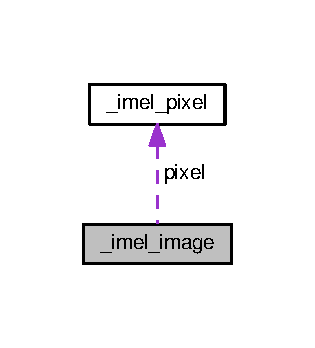
\includegraphics[width=151pt]{struct__imel__image__coll__graph}
\end{center}
\end{figure}
\subsection*{Data Fields}
{\bf }\par
\begin{DoxyCompactItemize}
\item 
\hyperlink{header_8h_af8a2b40c34eeed326846d0098ea84ec2}{Imel\+Size} \hyperlink{struct__imel__image_a21d117461b6a449755cf1519e6360be5}{width}
\item 
\hyperlink{header_8h_af8a2b40c34eeed326846d0098ea84ec2}{Imel\+Size} \hyperlink{struct__imel__image_aac8aaaa7bd52f888126f05cf87d46531}{height}
\item 
\hyperlink{header_8h_add7dd9f8c093208bc4fd135a22a670ba}{Imel\+Pixel} $\ast$$\ast$ \hyperlink{struct__imel__image_a7a156b8fc30a034d713afb77d198f320}{pixel}
\end{DoxyCompactItemize}



\subsection{Detailed Description}
Rappresentation of an image in Imel library. 

The most important type of Imel with \hyperlink{header_8h_add7dd9f8c093208bc4fd135a22a670ba}{Imel\+Pixel} is this. This type, in Imel, is an image which contains its resolution and its colors.

\begin{DoxySeeAlso}{See also}
\hyperlink{image_8c_af3a4abcb52f5611781065536fda0f97e}{imel\+\_\+image\+\_\+new} 

\hyperlink{image__new__from_8c_a43a15b507cf100b80bc07ce92a48adc7}{imel\+\_\+image\+\_\+new\+\_\+from} 
\end{DoxySeeAlso}


\subsection{Field Documentation}
\index{\+\_\+imel\+\_\+image@{\+\_\+imel\+\_\+image}!height@{height}}
\index{height@{height}!\+\_\+imel\+\_\+image@{\+\_\+imel\+\_\+image}}
\subsubsection[{\texorpdfstring{height}{height}}]{\setlength{\rightskip}{0pt plus 5cm}{\bf Imel\+Size} \+\_\+imel\+\_\+image\+::height}\hypertarget{struct__imel__image_aac8aaaa7bd52f888126f05cf87d46531}{}\label{struct__imel__image_aac8aaaa7bd52f888126f05cf87d46531}
Image height \index{\+\_\+imel\+\_\+image@{\+\_\+imel\+\_\+image}!pixel@{pixel}}
\index{pixel@{pixel}!\+\_\+imel\+\_\+image@{\+\_\+imel\+\_\+image}}
\subsubsection[{\texorpdfstring{pixel}{pixel}}]{\setlength{\rightskip}{0pt plus 5cm}{\bf Imel\+Pixel}$\ast$$\ast$ \+\_\+imel\+\_\+image\+::pixel}\hypertarget{struct__imel__image_a7a156b8fc30a034d713afb77d198f320}{}\label{struct__imel__image_a7a156b8fc30a034d713afb77d198f320}
2-\/dimensional array in \mbox{[}y\mbox{]}\mbox{[}x\mbox{]} format. \index{\+\_\+imel\+\_\+image@{\+\_\+imel\+\_\+image}!width@{width}}
\index{width@{width}!\+\_\+imel\+\_\+image@{\+\_\+imel\+\_\+image}}
\subsubsection[{\texorpdfstring{width}{width}}]{\setlength{\rightskip}{0pt plus 5cm}{\bf Imel\+Size} \+\_\+imel\+\_\+image\+::width}\hypertarget{struct__imel__image_a21d117461b6a449755cf1519e6360be5}{}\label{struct__imel__image_a21d117461b6a449755cf1519e6360be5}
Image width 

The documentation for this struct was generated from the following file\+:\begin{DoxyCompactItemize}
\item 
\hyperlink{header_8h}{header.\+h}\end{DoxyCompactItemize}

\hypertarget{struct__imel__info__cut}{}\section{\+\_\+imel\+\_\+info\+\_\+cut Struct Reference}
\label{struct__imel__info__cut}\index{\+\_\+imel\+\_\+info\+\_\+cut@{\+\_\+imel\+\_\+info\+\_\+cut}}


{\ttfamily \#include $<$header.\+h$>$}



Collaboration diagram for \+\_\+imel\+\_\+info\+\_\+cut\+:
\nopagebreak
\begin{figure}[H]
\begin{center}
\leavevmode
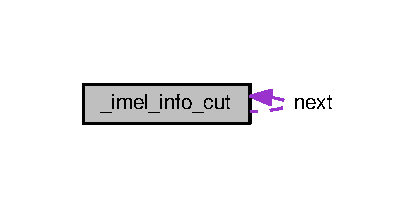
\includegraphics[width=200pt]{struct__imel__info__cut__coll__graph}
\end{center}
\end{figure}
\subsection*{Data Fields}
{\bf }\par
\begin{DoxyCompactItemize}
\item 
\hyperlink{header_8h_af8a2b40c34eeed326846d0098ea84ec2}{Imel\+Size} \hyperlink{struct__imel__info__cut_ae436b332b23852dd64b64b65b6410f64}{index}
\item 
\hyperlink{header_8h_aef27fcac7a96d118b3c3194c2577049f}{Imel\+Orientation} \hyperlink{struct__imel__info__cut_a3c2a7e5ecd568b3742a1ac0cdbc9ae9d}{orientation}
\item 
\hyperlink{header_8h_af8a2b40c34eeed326846d0098ea84ec2}{Imel\+Size} \hyperlink{struct__imel__info__cut_a6690e6207a17f6407ec469699bc5d7d0}{position}
\item 
struct \hyperlink{struct__imel__info__cut}{\+\_\+imel\+\_\+info\+\_\+cut} $\ast$ \hyperlink{struct__imel__info__cut_a3e0e1c8db6cdc22b7f4247e0b295a0d9}{next}
\end{DoxyCompactItemize}



\subsection{Detailed Description}
This type collect information about the hypothetical lines that cut an image vertically or horizontally at a specific point.

\begin{DoxySeeAlso}{See also}
\hyperlink{image_8c_a31943792f957de747e49b6dc1fbbab05}{imel\+\_\+image\+\_\+cut\+\_\+grid} 

\hyperlink{info__cut_8c_ad06ec44d23c494c1f501d03de880007e}{imel\+\_\+info\+\_\+cut\+\_\+new} 

\hyperlink{info__cut_8c_aa8e34152e2f5716e6a195ee1b8107f85}{imel\+\_\+info\+\_\+cut\+\_\+add} 

\hyperlink{info__cut_8c_a73ba0a29544436cf4248c71a935560cd}{imel\+\_\+info\+\_\+cut\+\_\+free} 
\end{DoxySeeAlso}


\subsection{Field Documentation}
\index{\+\_\+imel\+\_\+info\+\_\+cut@{\+\_\+imel\+\_\+info\+\_\+cut}!index@{index}}
\index{index@{index}!\+\_\+imel\+\_\+info\+\_\+cut@{\+\_\+imel\+\_\+info\+\_\+cut}}
\subsubsection[{\texorpdfstring{index}{index}}]{\setlength{\rightskip}{0pt plus 5cm}{\bf Imel\+Size} \+\_\+imel\+\_\+info\+\_\+cut\+::index}\hypertarget{struct__imel__info__cut_ae436b332b23852dd64b64b65b6410f64}{}\label{struct__imel__info__cut_ae436b332b23852dd64b64b65b6410f64}
Element index \index{\+\_\+imel\+\_\+info\+\_\+cut@{\+\_\+imel\+\_\+info\+\_\+cut}!next@{next}}
\index{next@{next}!\+\_\+imel\+\_\+info\+\_\+cut@{\+\_\+imel\+\_\+info\+\_\+cut}}
\subsubsection[{\texorpdfstring{next}{next}}]{\setlength{\rightskip}{0pt plus 5cm}struct {\bf \+\_\+imel\+\_\+info\+\_\+cut}$\ast$ \+\_\+imel\+\_\+info\+\_\+cut\+::next}\hypertarget{struct__imel__info__cut_a3e0e1c8db6cdc22b7f4247e0b295a0d9}{}\label{struct__imel__info__cut_a3e0e1c8db6cdc22b7f4247e0b295a0d9}
Next element \index{\+\_\+imel\+\_\+info\+\_\+cut@{\+\_\+imel\+\_\+info\+\_\+cut}!orientation@{orientation}}
\index{orientation@{orientation}!\+\_\+imel\+\_\+info\+\_\+cut@{\+\_\+imel\+\_\+info\+\_\+cut}}
\subsubsection[{\texorpdfstring{orientation}{orientation}}]{\setlength{\rightskip}{0pt plus 5cm}{\bf Imel\+Orientation} \+\_\+imel\+\_\+info\+\_\+cut\+::orientation}\hypertarget{struct__imel__info__cut_a3c2a7e5ecd568b3742a1ac0cdbc9ae9d}{}\label{struct__imel__info__cut_a3c2a7e5ecd568b3742a1ac0cdbc9ae9d}
Line orientation \index{\+\_\+imel\+\_\+info\+\_\+cut@{\+\_\+imel\+\_\+info\+\_\+cut}!position@{position}}
\index{position@{position}!\+\_\+imel\+\_\+info\+\_\+cut@{\+\_\+imel\+\_\+info\+\_\+cut}}
\subsubsection[{\texorpdfstring{position}{position}}]{\setlength{\rightskip}{0pt plus 5cm}{\bf Imel\+Size} \+\_\+imel\+\_\+info\+\_\+cut\+::position}\hypertarget{struct__imel__info__cut_a6690e6207a17f6407ec469699bc5d7d0}{}\label{struct__imel__info__cut_a6690e6207a17f6407ec469699bc5d7d0}
Line position 

The documentation for this struct was generated from the following file\+:\begin{DoxyCompactItemize}
\item 
\hyperlink{header_8h}{header.\+h}\end{DoxyCompactItemize}

\hypertarget{struct__imel__pixel}{}\section{\+\_\+imel\+\_\+pixel Struct Reference}
\label{struct__imel__pixel}\index{\+\_\+imel\+\_\+pixel@{\+\_\+imel\+\_\+pixel}}


Rappresentation of a pixel in Imel library.  




{\ttfamily \#include $<$header.\+h$>$}

\subsection*{Data Fields}
{\bf }\par
\begin{DoxyCompactItemize}
\item 
\hyperlink{header_8h_add1326f75f0c1a7da9f14c2ed4f673e9}{Imel\+Color} \hyperlink{struct__imel__pixel_af491601f44bd0b35d72b77f94940ec65}{red}
\item 
\hyperlink{header_8h_add1326f75f0c1a7da9f14c2ed4f673e9}{Imel\+Color} \hyperlink{struct__imel__pixel_a3776e5a017e15b9dfad83b90b58e982e}{green}
\item 
\hyperlink{header_8h_add1326f75f0c1a7da9f14c2ed4f673e9}{Imel\+Color} \hyperlink{struct__imel__pixel_a1e3b4f517f6a56b353f4ed58f880a08e}{blue}
\item 
\hyperlink{header_8h_a97bc4b146a807c2d83b966983132f4fc}{Imel\+Level} \hyperlink{struct__imel__pixel_a729d8e2d9902ac1a6e2fbbc6f63cf1ed}{level}
\end{DoxyCompactItemize}



\subsection{Detailed Description}
Rappresentation of a pixel in Imel library. 

This type is the fundamental one, includes all the information needed to create a pixel composed of the three basic colors and its importance or transparency.


\begin{DoxyCode}
\hyperlink{struct__imel__pixel}{ImelPixel} m1\_color = \{ 255, 255, 255, 0 \};
\hyperlink{struct__imel__pixel}{ImelPixel} m2\_color;

m2\_color = \hyperlink{pixel_8c_a0d1c4cb614847e8084854f40d05d0eb7}{imel\_pixel\_new\_from\_string} (\textcolor{stringliteral}{'#ffffff'}, 0);
\end{DoxyCode}


\begin{DoxySeeAlso}{See also}
\hyperlink{pixel_8c_aaf2dba6a30b6612b7c1730195935a88d}{imel\+\_\+pixel\+\_\+new} 

\hyperlink{pixel_8c_a0d1c4cb614847e8084854f40d05d0eb7}{imel\+\_\+pixel\+\_\+new\+\_\+from\+\_\+string} 

\hyperlink{pixel_8c_af701f338fec84020c7e812f7c1eb84df}{imel\+\_\+pixel\+\_\+new\+\_\+from\+\_\+rgba} 

\hyperlink{pixel_8c_a8ba2bb2ac90703240cd2c7556a4b9680}{imel\+\_\+pixel\+\_\+new\+\_\+from\+\_\+hsl} 

\hyperlink{pixel_8c_a9bc6aa8b3ec663f1635827b0ebbdf46a}{imel\+\_\+pixel\+\_\+copy}
\end{DoxySeeAlso}
\begin{DoxyNote}{Note}
If two pixels have different level values when they are used in functions like \hyperlink{pixel_8c_a9bc6aa8b3ec663f1635827b0ebbdf46a}{imel\+\_\+pixel\+\_\+copy} the first one can be replaced only if the second one has the same or greater level value. 
\end{DoxyNote}


\subsection{Field Documentation}
\index{\+\_\+imel\+\_\+pixel@{\+\_\+imel\+\_\+pixel}!blue@{blue}}
\index{blue@{blue}!\+\_\+imel\+\_\+pixel@{\+\_\+imel\+\_\+pixel}}
\subsubsection[{\texorpdfstring{blue}{blue}}]{\setlength{\rightskip}{0pt plus 5cm}{\bf Imel\+Color} \+\_\+imel\+\_\+pixel\+::blue}\hypertarget{struct__imel__pixel_a1e3b4f517f6a56b353f4ed58f880a08e}{}\label{struct__imel__pixel_a1e3b4f517f6a56b353f4ed58f880a08e}
Blue channel. Values from 0 to 255. \index{\+\_\+imel\+\_\+pixel@{\+\_\+imel\+\_\+pixel}!green@{green}}
\index{green@{green}!\+\_\+imel\+\_\+pixel@{\+\_\+imel\+\_\+pixel}}
\subsubsection[{\texorpdfstring{green}{green}}]{\setlength{\rightskip}{0pt plus 5cm}{\bf Imel\+Color} \+\_\+imel\+\_\+pixel\+::green}\hypertarget{struct__imel__pixel_a3776e5a017e15b9dfad83b90b58e982e}{}\label{struct__imel__pixel_a3776e5a017e15b9dfad83b90b58e982e}
Green channel. Values from 0 to 255. \index{\+\_\+imel\+\_\+pixel@{\+\_\+imel\+\_\+pixel}!level@{level}}
\index{level@{level}!\+\_\+imel\+\_\+pixel@{\+\_\+imel\+\_\+pixel}}
\subsubsection[{\texorpdfstring{level}{level}}]{\setlength{\rightskip}{0pt plus 5cm}{\bf Imel\+Level} \+\_\+imel\+\_\+pixel\+::level}\hypertarget{struct__imel__pixel_a729d8e2d9902ac1a6e2fbbc6f63cf1ed}{}\label{struct__imel__pixel_a729d8e2d9902ac1a6e2fbbc6f63cf1ed}
Alpha for values from 0 to -\/255, else level \index{\+\_\+imel\+\_\+pixel@{\+\_\+imel\+\_\+pixel}!red@{red}}
\index{red@{red}!\+\_\+imel\+\_\+pixel@{\+\_\+imel\+\_\+pixel}}
\subsubsection[{\texorpdfstring{red}{red}}]{\setlength{\rightskip}{0pt plus 5cm}{\bf Imel\+Color} \+\_\+imel\+\_\+pixel\+::red}\hypertarget{struct__imel__pixel_af491601f44bd0b35d72b77f94940ec65}{}\label{struct__imel__pixel_af491601f44bd0b35d72b77f94940ec65}
Red channel. Values from 0 to 255. 

The documentation for this struct was generated from the following file\+:\begin{DoxyCompactItemize}
\item 
\hyperlink{header_8h}{header.\+h}\end{DoxyCompactItemize}

\hypertarget{struct__imel__point}{}\section{\+\_\+imel\+\_\+point Struct Reference}
\label{struct__imel__point}\index{\+\_\+imel\+\_\+point@{\+\_\+imel\+\_\+point}}


Rappresentation of a point in Imel library.  




{\ttfamily \#include $<$header.\+h$>$}



Collaboration diagram for \+\_\+imel\+\_\+point\+:
\nopagebreak
\begin{figure}[H]
\begin{center}
\leavevmode
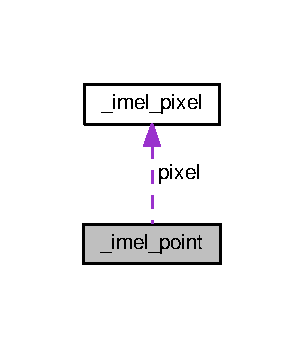
\includegraphics[width=146pt]{struct__imel__point__coll__graph}
\end{center}
\end{figure}
\subsection*{Data Fields}
{\bf }\par
\begin{DoxyCompactItemize}
\item 
\hyperlink{header_8h_af8a2b40c34eeed326846d0098ea84ec2}{Imel\+Size} \hyperlink{struct__imel__point_ae691eec1e0fdf37d07d13d44a0e0539c}{x}
\item 
\hyperlink{header_8h_af8a2b40c34eeed326846d0098ea84ec2}{Imel\+Size} \hyperlink{struct__imel__point_a30dc84507e749f7157cecd08cb045b4e}{y}
\item 
\hyperlink{header_8h_add7dd9f8c093208bc4fd135a22a670ba}{Imel\+Pixel} \hyperlink{struct__imel__point_af4b99377296131681a16ab67599c152b}{pixel}
\end{DoxyCompactItemize}



\subsection{Detailed Description}
Rappresentation of a point in Imel library. 

This type can rappresent a point with coordinates, color and level.

\begin{DoxySeeAlso}{See also}
\hyperlink{point_8c_a20c030176364130df49237e29b69308c}{imel\+\_\+point\+\_\+new} 
\end{DoxySeeAlso}


\subsection{Field Documentation}
\index{\+\_\+imel\+\_\+point@{\+\_\+imel\+\_\+point}!pixel@{pixel}}
\index{pixel@{pixel}!\+\_\+imel\+\_\+point@{\+\_\+imel\+\_\+point}}
\subsubsection[{\texorpdfstring{pixel}{pixel}}]{\setlength{\rightskip}{0pt plus 5cm}{\bf Imel\+Pixel} \+\_\+imel\+\_\+point\+::pixel}\hypertarget{struct__imel__point_af4b99377296131681a16ab67599c152b}{}\label{struct__imel__point_af4b99377296131681a16ab67599c152b}
Color and level of the point \index{\+\_\+imel\+\_\+point@{\+\_\+imel\+\_\+point}!x@{x}}
\index{x@{x}!\+\_\+imel\+\_\+point@{\+\_\+imel\+\_\+point}}
\subsubsection[{\texorpdfstring{x}{x}}]{\setlength{\rightskip}{0pt plus 5cm}{\bf Imel\+Size} \+\_\+imel\+\_\+point\+::x}\hypertarget{struct__imel__point_ae691eec1e0fdf37d07d13d44a0e0539c}{}\label{struct__imel__point_ae691eec1e0fdf37d07d13d44a0e0539c}
Coordinate x \index{\+\_\+imel\+\_\+point@{\+\_\+imel\+\_\+point}!y@{y}}
\index{y@{y}!\+\_\+imel\+\_\+point@{\+\_\+imel\+\_\+point}}
\subsubsection[{\texorpdfstring{y}{y}}]{\setlength{\rightskip}{0pt plus 5cm}{\bf Imel\+Size} \+\_\+imel\+\_\+point\+::y}\hypertarget{struct__imel__point_a30dc84507e749f7157cecd08cb045b4e}{}\label{struct__imel__point_a30dc84507e749f7157cecd08cb045b4e}
Coordinate y 

The documentation for this struct was generated from the following file\+:\begin{DoxyCompactItemize}
\item 
\hyperlink{header_8h}{header.\+h}\end{DoxyCompactItemize}

\chapter{File Documentation}
\hypertarget{color_8c}{}\section{color.\+c File Reference}
\label{color_8c}\index{color.\+c@{color.\+c}}


This file contains functions to operate with colors.  


{\ttfamily \#include $<$stdlib.\+h$>$}\\*
{\ttfamily \#include \char`\"{}header.\+h\char`\"{}}\\*
Include dependency graph for color.\+c\+:
\nopagebreak
\begin{figure}[H]
\begin{center}
\leavevmode
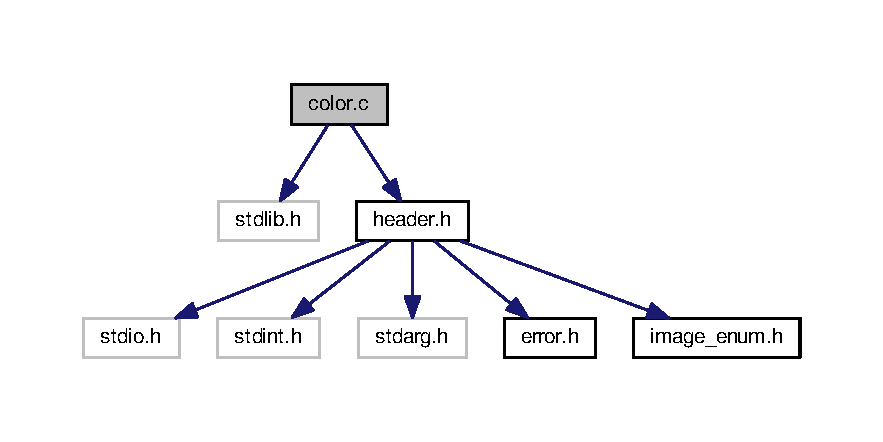
\includegraphics[width=350pt]{color_8c__incl}
\end{center}
\end{figure}
\subsection*{Functions}
\begin{DoxyCompactItemize}
\item 
void \hyperlink{color_8c_a683618c6373e0b3408b62eb2ad66bed0}{imel\+\_\+color\+\_\+set\+\_\+background} (\hyperlink{header_8h_ad8298d38a89742ed84029b278c6acee5}{Imel\+Image} $\ast$image, \hyperlink{header_8h_add7dd9f8c093208bc4fd135a22a670ba}{Imel\+Pixel} pixel)
\begin{DoxyCompactList}\small\item\em Sets a background color to a chosen image. \end{DoxyCompactList}\item 
\hyperlink{header_8h_add7dd9f8c093208bc4fd135a22a670ba}{Imel\+Pixel} $\ast$$\ast$ \hyperlink{color_8c_aed504db1eeedb03f0042a8983de1881c}{imel\+\_\+color\+\_\+get\+\_\+number} (\hyperlink{header_8h_ad8298d38a89742ed84029b278c6acee5}{Imel\+Image} $\ast$image, \hyperlink{header_8h_af8a2b40c34eeed326846d0098ea84ec2}{Imel\+Size} $\ast$number)
\begin{DoxyCompactList}\small\item\em Gets a list of unique colors in an image. \end{DoxyCompactList}\item 
\hyperlink{header_8h_add1326f75f0c1a7da9f14c2ed4f673e9}{Imel\+Color} $\ast$ \hyperlink{color_8c_a4cbbac29a4bacd39beaaf01eee111b0e}{imel\+\_\+color\+\_\+get\+\_\+from\+\_\+pixel} (\hyperlink{header_8h_add7dd9f8c093208bc4fd135a22a670ba}{Imel\+Pixel} pixel)
\begin{DoxyCompactList}\small\item\em Gets an array with the colors in a pixel. \end{DoxyCompactList}\item 
\hyperlink{header_8h_add1326f75f0c1a7da9f14c2ed4f673e9}{Imel\+Color} \hyperlink{color_8c_a27a789b40d98e5ea558eb6b37d752e01}{imel\+\_\+color\+\_\+sum} (\hyperlink{header_8h_add1326f75f0c1a7da9f14c2ed4f673e9}{Imel\+Color} a, \hyperlink{header_8h_add1326f75f0c1a7da9f14c2ed4f673e9}{Imel\+Color} b)
\begin{DoxyCompactList}\small\item\em Sum two colors. \end{DoxyCompactList}\item 
\hyperlink{header_8h_add1326f75f0c1a7da9f14c2ed4f673e9}{Imel\+Color} \hyperlink{color_8c_a94e41b5ec4f9170933fc108cea098c35}{imel\+\_\+color\+\_\+subtract} (\hyperlink{header_8h_add1326f75f0c1a7da9f14c2ed4f673e9}{Imel\+Color} a, \hyperlink{header_8h_add1326f75f0c1a7da9f14c2ed4f673e9}{Imel\+Color} b)
\begin{DoxyCompactList}\small\item\em Subtract two colors. \end{DoxyCompactList}\end{DoxyCompactItemize}


\subsection{Detailed Description}
This file contains functions to operate with colors. 

\begin{DoxyAuthor}{Author}
Davide Francesco Merico These functions allow you to add, subtract or extract information relative to the colors inside Imel types. 
\end{DoxyAuthor}


\subsection{Function Documentation}
\index{color.\+c@{color.\+c}!imel\+\_\+color\+\_\+get\+\_\+from\+\_\+pixel@{imel\+\_\+color\+\_\+get\+\_\+from\+\_\+pixel}}
\index{imel\+\_\+color\+\_\+get\+\_\+from\+\_\+pixel@{imel\+\_\+color\+\_\+get\+\_\+from\+\_\+pixel}!color.\+c@{color.\+c}}
\subsubsection[{\texorpdfstring{imel\+\_\+color\+\_\+get\+\_\+from\+\_\+pixel(\+Imel\+Pixel pixel)}{imel_color_get_from_pixel(ImelPixel pixel)}}]{\setlength{\rightskip}{0pt plus 5cm}{\bf Imel\+Color}$\ast$ imel\+\_\+color\+\_\+get\+\_\+from\+\_\+pixel (
\begin{DoxyParamCaption}
\item[{{\bf Imel\+Pixel}}]{pixel}
\end{DoxyParamCaption}
)}\hypertarget{color_8c_a4cbbac29a4bacd39beaaf01eee111b0e}{}\label{color_8c_a4cbbac29a4bacd39beaaf01eee111b0e}


Gets an array with the colors in a pixel. 

This function make a color array with rgb value in {\ttfamily pixel}.


\begin{DoxyParams}{Parameters}
{\em pixel} & Pixel from which get the colors. \\
\hline
\end{DoxyParams}
\begin{DoxyReturn}{Returns}
An array with R\+GB channels of {\ttfamily pixel}. 
\end{DoxyReturn}
\begin{DoxyNote}{Note}
Each channel can be setted to 0 if {\ttfamily pixel} level is less then -\/255. 
\end{DoxyNote}
\index{color.\+c@{color.\+c}!imel\+\_\+color\+\_\+get\+\_\+number@{imel\+\_\+color\+\_\+get\+\_\+number}}
\index{imel\+\_\+color\+\_\+get\+\_\+number@{imel\+\_\+color\+\_\+get\+\_\+number}!color.\+c@{color.\+c}}
\subsubsection[{\texorpdfstring{imel\+\_\+color\+\_\+get\+\_\+number(\+Imel\+Image $\ast$image, Imel\+Size $\ast$number)}{imel_color_get_number(ImelImage *image, ImelSize *number)}}]{\setlength{\rightskip}{0pt plus 5cm}{\bf Imel\+Pixel}$\ast$$\ast$ imel\+\_\+color\+\_\+get\+\_\+number (
\begin{DoxyParamCaption}
\item[{{\bf Imel\+Image} $\ast$}]{image, }
\item[{{\bf Imel\+Size} $\ast$}]{number}
\end{DoxyParamCaption}
)}\hypertarget{color_8c_aed504db1eeedb03f0042a8983de1881c}{}\label{color_8c_aed504db1eeedb03f0042a8983de1881c}


Gets a list of unique colors in an image. 

This function get the unique colors number in {\ttfamily image} and return a list of this colors.


\begin{DoxyCode}
1 ImelImage *image = imel\_image\_new\_from ("image.png", 0, NULL);
2 ImelSize n\_colors;
3 ImelPixel *list;
4 
5 list = imel\_color\_get\_number (image, &n\_colors);
6 ...
7 free (list);
\end{DoxyCode}



\begin{DoxyParams}{Parameters}
{\em image} & Image from which exract the colors \\
\hline
{\em number} & In this variabile can be saved the colors number \\
\hline
\end{DoxyParams}
\begin{DoxyReturn}{Returns}
N\+U\+LL if {\ttfamily image} isn\textquotesingle{}t valid, else a N\+U\+L\+L-\/terminated list with the found colors. 
\end{DoxyReturn}
\begin{DoxyWarning}{Warning}
Each pixel of the returned list is linked to an {\ttfamily image} pixel, to free memory call free only on list as in example above. 
\end{DoxyWarning}
\index{color.\+c@{color.\+c}!imel\+\_\+color\+\_\+set\+\_\+background@{imel\+\_\+color\+\_\+set\+\_\+background}}
\index{imel\+\_\+color\+\_\+set\+\_\+background@{imel\+\_\+color\+\_\+set\+\_\+background}!color.\+c@{color.\+c}}
\subsubsection[{\texorpdfstring{imel\+\_\+color\+\_\+set\+\_\+background(\+Imel\+Image $\ast$image, Imel\+Pixel pixel)}{imel_color_set_background(ImelImage *image, ImelPixel pixel)}}]{\setlength{\rightskip}{0pt plus 5cm}void imel\+\_\+color\+\_\+set\+\_\+background (
\begin{DoxyParamCaption}
\item[{{\bf Imel\+Image} $\ast$}]{image, }
\item[{{\bf Imel\+Pixel}}]{pixel}
\end{DoxyParamCaption}
)}\hypertarget{color_8c_a683618c6373e0b3408b62eb2ad66bed0}{}\label{color_8c_a683618c6373e0b3408b62eb2ad66bed0}


Sets a background color to a chosen image. 

This function copy through \hyperlink{pixel_8c_a9bc6aa8b3ec663f1635827b0ebbdf46a}{imel\+\_\+pixel\+\_\+copy} {\ttfamily pixel} in each pixel of {\ttfamily image}.


\begin{DoxyCode}
1 ImelImage *image = imel\_image\_new\_from ("image.gif", 0, NULL);
2 ImelPixel bg\_pixel = \{ 255, 255, 255, 0 \};
3 
4 imel\_color\_set\_background (image, bg\_pixel);
\end{DoxyCode}



\begin{DoxyParams}{Parameters}
{\em image} & Image to set a new background \\
\hline
{\em pixel} & Background color\\
\hline
\end{DoxyParams}
\begin{DoxySeeAlso}{See also}
\hyperlink{pixel_8c_a9bc6aa8b3ec663f1635827b0ebbdf46a}{imel\+\_\+pixel\+\_\+copy} 
\end{DoxySeeAlso}
\index{color.\+c@{color.\+c}!imel\+\_\+color\+\_\+subtract@{imel\+\_\+color\+\_\+subtract}}
\index{imel\+\_\+color\+\_\+subtract@{imel\+\_\+color\+\_\+subtract}!color.\+c@{color.\+c}}
\subsubsection[{\texorpdfstring{imel\+\_\+color\+\_\+subtract(\+Imel\+Color a, Imel\+Color b)}{imel_color_subtract(ImelColor a, ImelColor b)}}]{\setlength{\rightskip}{0pt plus 5cm}{\bf Imel\+Color} imel\+\_\+color\+\_\+subtract (
\begin{DoxyParamCaption}
\item[{{\bf Imel\+Color}}]{a, }
\item[{{\bf Imel\+Color}}]{b}
\end{DoxyParamCaption}
)}\hypertarget{color_8c_a94e41b5ec4f9170933fc108cea098c35}{}\label{color_8c_a94e41b5ec4f9170933fc108cea098c35}


Subtract two colors. 

This function subtract {\ttfamily b} from {\ttfamily a}.


\begin{DoxyParams}{Parameters}
{\em a} & First color \\
\hline
{\em b} & Second color \\
\hline
\end{DoxyParams}
\begin{DoxyReturn}{Returns}
A color with the result of {\ttfamily b} -\/ {\ttfamily a}, if the result is less then 0 return 0. 
\end{DoxyReturn}
\index{color.\+c@{color.\+c}!imel\+\_\+color\+\_\+sum@{imel\+\_\+color\+\_\+sum}}
\index{imel\+\_\+color\+\_\+sum@{imel\+\_\+color\+\_\+sum}!color.\+c@{color.\+c}}
\subsubsection[{\texorpdfstring{imel\+\_\+color\+\_\+sum(\+Imel\+Color a, Imel\+Color b)}{imel_color_sum(ImelColor a, ImelColor b)}}]{\setlength{\rightskip}{0pt plus 5cm}{\bf Imel\+Color} imel\+\_\+color\+\_\+sum (
\begin{DoxyParamCaption}
\item[{{\bf Imel\+Color}}]{a, }
\item[{{\bf Imel\+Color}}]{b}
\end{DoxyParamCaption}
)}\hypertarget{color_8c_a27a789b40d98e5ea558eb6b37d752e01}{}\label{color_8c_a27a789b40d98e5ea558eb6b37d752e01}


Sum two colors. 

This function sum colors {\ttfamily a} and {\ttfamily b}.


\begin{DoxyParams}{Parameters}
{\em a} & First color \\
\hline
{\em b} & Second color \\
\hline
\end{DoxyParams}
\begin{DoxyReturn}{Returns}
A color with the sum of {\ttfamily a} and {\ttfamily b}, if the sum result is greater then 255 return 255. 
\end{DoxyReturn}

\hypertarget{draw_8c}{}\section{draw.\+c File Reference}
\label{draw_8c}\index{draw.\+c@{draw.\+c}}


This file contains functions to draw.  


{\ttfamily \#include $<$string.\+h$>$}\\*
{\ttfamily \#include $<$stdlib.\+h$>$}\\*
{\ttfamily \#include $<$math.\+h$>$}\\*
{\ttfamily \#include \char`\"{}header.\+h\char`\"{}}\\*
Include dependency graph for draw.\+c\+:
\nopagebreak
\begin{figure}[H]
\begin{center}
\leavevmode
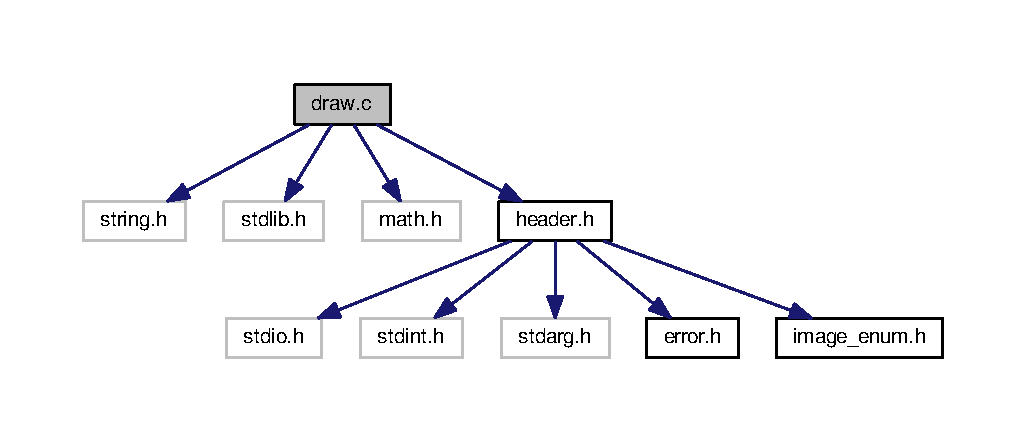
\includegraphics[width=350pt]{draw_8c__incl}
\end{center}
\end{figure}
\subsection*{Functions}
\begin{DoxyCompactItemize}
\item 
void \hyperlink{draw_8c_a3e8d240e5d85197b6070f0ec97b2c030}{imel\+\_\+draw\+\_\+circle} (\hyperlink{header_8h_ad8298d38a89742ed84029b278c6acee5}{Imel\+Image} $\ast$image, \hyperlink{header_8h_af8a2b40c34eeed326846d0098ea84ec2}{Imel\+Size} x, \hyperlink{header_8h_af8a2b40c34eeed326846d0098ea84ec2}{Imel\+Size} y, \hyperlink{header_8h_af8a2b40c34eeed326846d0098ea84ec2}{Imel\+Size} radius, \hyperlink{header_8h_add7dd9f8c093208bc4fd135a22a670ba}{Imel\+Pixel} pxl)
\begin{DoxyCompactList}\small\item\em Draw a circle. \end{DoxyCompactList}\item 
\hyperlink{header_8h_a669b28ed18156f1a4f13732e070d6cf2}{bool} \hyperlink{draw_8c_ad8b931ece29f161af9b5a4153d186dd4}{imel\+\_\+draw\+\_\+partial\+\_\+reg\+\_\+shape} (\hyperlink{header_8h_ad8298d38a89742ed84029b278c6acee5}{Imel\+Image} $\ast$image, \hyperlink{header_8h_af8a2b40c34eeed326846d0098ea84ec2}{Imel\+Size} x, \hyperlink{header_8h_af8a2b40c34eeed326846d0098ea84ec2}{Imel\+Size} y, \hyperlink{header_8h_af8a2b40c34eeed326846d0098ea84ec2}{Imel\+Size} r, long v, short p, double start\+\_\+angle, \hyperlink{header_8h_add7dd9f8c093208bc4fd135a22a670ba}{Imel\+Pixel} pxl)
\begin{DoxyCompactList}\small\item\em Draw a partial regular shape. \end{DoxyCompactList}\item 
\hyperlink{header_8h_a669b28ed18156f1a4f13732e070d6cf2}{bool} \hyperlink{draw_8c_a4cc27abce5f2d1cfe72dc7e5b078adc8}{imel\+\_\+draw\+\_\+arch} (\hyperlink{header_8h_ad8298d38a89742ed84029b278c6acee5}{Imel\+Image} $\ast$image, \hyperlink{header_8h_af8a2b40c34eeed326846d0098ea84ec2}{Imel\+Size} x, \hyperlink{header_8h_af8a2b40c34eeed326846d0098ea84ec2}{Imel\+Size} y, \hyperlink{header_8h_af8a2b40c34eeed326846d0098ea84ec2}{Imel\+Size} radius, double start\+\_\+angle, double end\+\_\+angle, \hyperlink{header_8h_add7dd9f8c093208bc4fd135a22a670ba}{Imel\+Pixel} pxl)
\begin{DoxyCompactList}\small\item\em Draw an arch. \end{DoxyCompactList}\item 
\hyperlink{header_8h_a669b28ed18156f1a4f13732e070d6cf2}{bool} \hyperlink{draw_8c_ac7a6615ed3eeda8f99766116040a86e9}{imel\+\_\+draw\+\_\+filled\+\_\+arch} (\hyperlink{header_8h_ad8298d38a89742ed84029b278c6acee5}{Imel\+Image} $\ast$image, \hyperlink{header_8h_af8a2b40c34eeed326846d0098ea84ec2}{Imel\+Size} x, \hyperlink{header_8h_af8a2b40c34eeed326846d0098ea84ec2}{Imel\+Size} y, \hyperlink{header_8h_af8a2b40c34eeed326846d0098ea84ec2}{Imel\+Size} radius, double start\+\_\+angle, double end\+\_\+angle, \hyperlink{header_8h_add7dd9f8c093208bc4fd135a22a670ba}{Imel\+Pixel} pxl)
\begin{DoxyCompactList}\small\item\em Draw a filled arch. \end{DoxyCompactList}\item 
\hyperlink{header_8h_a669b28ed18156f1a4f13732e070d6cf2}{bool} \hyperlink{draw_8c_a0168dd78ad67c50479e3244c9f6cc2a6}{imel\+\_\+draw\+\_\+line} (\hyperlink{header_8h_ad8298d38a89742ed84029b278c6acee5}{Imel\+Image} $\ast$image, \hyperlink{header_8h_af8a2b40c34eeed326846d0098ea84ec2}{Imel\+Size} \+\_\+sx, \hyperlink{header_8h_af8a2b40c34eeed326846d0098ea84ec2}{Imel\+Size} \+\_\+sy, \hyperlink{header_8h_af8a2b40c34eeed326846d0098ea84ec2}{Imel\+Size} \+\_\+ex, \hyperlink{header_8h_af8a2b40c34eeed326846d0098ea84ec2}{Imel\+Size} \+\_\+ey, \hyperlink{header_8h_add7dd9f8c093208bc4fd135a22a670ba}{Imel\+Pixel} pixel)
\begin{DoxyCompactList}\small\item\em Draw a line. \end{DoxyCompactList}\item 
void \hyperlink{draw_8c_a80e6d667aceb3de202823e5493a774b1}{imel\+\_\+draw\+\_\+point} (\hyperlink{header_8h_ad8298d38a89742ed84029b278c6acee5}{Imel\+Image} $\ast$image, \hyperlink{header_8h_af8a2b40c34eeed326846d0098ea84ec2}{Imel\+Size} x, \hyperlink{header_8h_af8a2b40c34eeed326846d0098ea84ec2}{Imel\+Size} y, \hyperlink{header_8h_add7dd9f8c093208bc4fd135a22a670ba}{Imel\+Pixel} pixel)
\begin{DoxyCompactList}\small\item\em Draw a single point in an image. \end{DoxyCompactList}\item 
void \hyperlink{draw_8c_a9d6234ac96cccab2e2d6b36acc78a865}{imel\+\_\+draw\+\_\+filled\+\_\+circle} (\hyperlink{header_8h_ad8298d38a89742ed84029b278c6acee5}{Imel\+Image} $\ast$image, \hyperlink{header_8h_af8a2b40c34eeed326846d0098ea84ec2}{Imel\+Size} x, \hyperlink{header_8h_af8a2b40c34eeed326846d0098ea84ec2}{Imel\+Size} y, \hyperlink{header_8h_af8a2b40c34eeed326846d0098ea84ec2}{Imel\+Size} radius, \hyperlink{header_8h_add7dd9f8c093208bc4fd135a22a670ba}{Imel\+Pixel} pxl)
\begin{DoxyCompactList}\small\item\em Draw a filled circle. \end{DoxyCompactList}\item 
void \hyperlink{draw_8c_aa6c826f436252a630b7e4d1d10c73309}{imel\+\_\+draw\+\_\+rect} (\hyperlink{header_8h_ad8298d38a89742ed84029b278c6acee5}{Imel\+Image} $\ast$image, \hyperlink{header_8h_af8a2b40c34eeed326846d0098ea84ec2}{Imel\+Size} x1, \hyperlink{header_8h_af8a2b40c34eeed326846d0098ea84ec2}{Imel\+Size} y1, \hyperlink{header_8h_af8a2b40c34eeed326846d0098ea84ec2}{Imel\+Size} x2, \hyperlink{header_8h_af8a2b40c34eeed326846d0098ea84ec2}{Imel\+Size} y2, \hyperlink{header_8h_add7dd9f8c093208bc4fd135a22a670ba}{Imel\+Pixel} pixel, \hyperlink{header_8h_a669b28ed18156f1a4f13732e070d6cf2}{bool} fill)
\begin{DoxyCompactList}\small\item\em Draw a rectangle ( filled or not ) \end{DoxyCompactList}\item 
\hyperlink{header_8h_a669b28ed18156f1a4f13732e070d6cf2}{bool} \hyperlink{draw_8c_a72fb4e6cce353b8051c269d89460cd1c}{imel\+\_\+draw\+\_\+rect\+\_\+with\+\_\+rounded\+\_\+angles} (\hyperlink{header_8h_ad8298d38a89742ed84029b278c6acee5}{Imel\+Image} $\ast$image, \hyperlink{header_8h_af8a2b40c34eeed326846d0098ea84ec2}{Imel\+Size} x1, \hyperlink{header_8h_af8a2b40c34eeed326846d0098ea84ec2}{Imel\+Size} y1, \hyperlink{header_8h_af8a2b40c34eeed326846d0098ea84ec2}{Imel\+Size} x2, \hyperlink{header_8h_af8a2b40c34eeed326846d0098ea84ec2}{Imel\+Size} y2, \hyperlink{header_8h_af8a2b40c34eeed326846d0098ea84ec2}{Imel\+Size} radius, \hyperlink{header_8h_add7dd9f8c093208bc4fd135a22a670ba}{Imel\+Pixel} pixel, \hyperlink{header_8h_a669b28ed18156f1a4f13732e070d6cf2}{bool} fill)
\begin{DoxyCompactList}\small\item\em Draw a rectangle with rounded angles ( filled or not ) \end{DoxyCompactList}\item 
void \hyperlink{draw_8c_a0f6a2052074967fa5b57e487544f42ee}{imel\+\_\+draw\+\_\+point\+\_\+from\+\_\+array} (\hyperlink{header_8h_ad8298d38a89742ed84029b278c6acee5}{Imel\+Image} $\ast$image, \hyperlink{header_8h_af8a2b40c34eeed326846d0098ea84ec2}{Imel\+Size} n\+\_\+points, \hyperlink{header_8h_a8b81d020f830e116585b833ea21410c1}{Imel\+Point} $\ast$$\ast$points)
\begin{DoxyCompactList}\small\item\em Draw more point at the same time. \end{DoxyCompactList}\item 
void \hyperlink{draw_8c_a6e85b1251f6fe37a3fd75e2642ef7d10}{imel\+\_\+draw\+\_\+ellipse} (\hyperlink{header_8h_ad8298d38a89742ed84029b278c6acee5}{Imel\+Image} $\ast$image, \hyperlink{header_8h_af8a2b40c34eeed326846d0098ea84ec2}{Imel\+Size} x, \hyperlink{header_8h_af8a2b40c34eeed326846d0098ea84ec2}{Imel\+Size} y, double a, double b, \hyperlink{header_8h_add7dd9f8c093208bc4fd135a22a670ba}{Imel\+Pixel} pxl)
\begin{DoxyCompactList}\small\item\em Draw an ellipse. \end{DoxyCompactList}\item 
void \hyperlink{draw_8c_a9e9f3690fd2cb70848b39036a1fe9745}{imel\+\_\+draw\+\_\+filled\+\_\+ellipse} (\hyperlink{header_8h_ad8298d38a89742ed84029b278c6acee5}{Imel\+Image} $\ast$image, \hyperlink{header_8h_af8a2b40c34eeed326846d0098ea84ec2}{Imel\+Size} x, \hyperlink{header_8h_af8a2b40c34eeed326846d0098ea84ec2}{Imel\+Size} y, double a, double b, \hyperlink{header_8h_add7dd9f8c093208bc4fd135a22a670ba}{Imel\+Pixel} pxl)
\begin{DoxyCompactList}\small\item\em Draw a filled ellipse. \end{DoxyCompactList}\item 
\hyperlink{header_8h_a669b28ed18156f1a4f13732e070d6cf2}{bool} \hyperlink{draw_8c_a0f17ca4ca8df8aada79f12e7cbd2397b}{imel\+\_\+draw\+\_\+gradient\+\_\+line} (\hyperlink{header_8h_ad8298d38a89742ed84029b278c6acee5}{Imel\+Image} $\ast$image, \hyperlink{header_8h_af8a2b40c34eeed326846d0098ea84ec2}{Imel\+Size} \+\_\+x1, \hyperlink{header_8h_af8a2b40c34eeed326846d0098ea84ec2}{Imel\+Size} \+\_\+y1, \hyperlink{header_8h_af8a2b40c34eeed326846d0098ea84ec2}{Imel\+Size} \+\_\+x2, \hyperlink{header_8h_af8a2b40c34eeed326846d0098ea84ec2}{Imel\+Size} \+\_\+y2, \hyperlink{header_8h_add7dd9f8c093208bc4fd135a22a670ba}{Imel\+Pixel} start, \hyperlink{header_8h_add7dd9f8c093208bc4fd135a22a670ba}{Imel\+Pixel} end)
\begin{DoxyCompactList}\small\item\em Draw a line with gradient. \end{DoxyCompactList}\item 
\hyperlink{header_8h_a669b28ed18156f1a4f13732e070d6cf2}{bool} \hyperlink{draw_8c_a538f52427d2d8f84b45e5570d1dbf080}{imel\+\_\+draw\+\_\+filled\+\_\+line} (\hyperlink{header_8h_ad8298d38a89742ed84029b278c6acee5}{Imel\+Image} $\ast$image, \hyperlink{header_8h_af8a2b40c34eeed326846d0098ea84ec2}{Imel\+Size} \+\_\+x1, \hyperlink{header_8h_af8a2b40c34eeed326846d0098ea84ec2}{Imel\+Size} \+\_\+y1, \hyperlink{header_8h_af8a2b40c34eeed326846d0098ea84ec2}{Imel\+Size} \+\_\+x2, \hyperlink{header_8h_af8a2b40c34eeed326846d0098ea84ec2}{Imel\+Size} \+\_\+y2, \hyperlink{header_8h_af8a2b40c34eeed326846d0098ea84ec2}{Imel\+Size} ox, \hyperlink{header_8h_af8a2b40c34eeed326846d0098ea84ec2}{Imel\+Size} oy, \hyperlink{header_8h_add7dd9f8c093208bc4fd135a22a670ba}{Imel\+Pixel} pixel)
\begin{DoxyCompactList}\small\item\em Draw a filled line. \end{DoxyCompactList}\item 
void \hyperlink{draw_8c_a2269fedea0f39513774d343c09587f2a}{imel\+\_\+draw\+\_\+figure} (\hyperlink{header_8h_ad8298d38a89742ed84029b278c6acee5}{Imel\+Image} $\ast$image, \hyperlink{header_8h_af8a2b40c34eeed326846d0098ea84ec2}{Imel\+Size} n\+\_\+points, \hyperlink{header_8h_a8b81d020f830e116585b833ea21410c1}{Imel\+Point} $\ast$$\ast$starts, \hyperlink{header_8h_a8b81d020f830e116585b833ea21410c1}{Imel\+Point} $\ast$$\ast$ends, \hyperlink{header_8h_add7dd9f8c093208bc4fd135a22a670ba}{Imel\+Pixel} pixel)
\begin{DoxyCompactList}\small\item\em Draw a non contiguous figure. \end{DoxyCompactList}\item 
void \hyperlink{draw_8c_a8fc23d2f1a63119c89e2d8e20acad3e5}{imel\+\_\+draw\+\_\+contiguous\+\_\+figure} (\hyperlink{header_8h_ad8298d38a89742ed84029b278c6acee5}{Imel\+Image} $\ast$image, \hyperlink{header_8h_af8a2b40c34eeed326846d0098ea84ec2}{Imel\+Size} n\+\_\+points, \hyperlink{header_8h_a8b81d020f830e116585b833ea21410c1}{Imel\+Point} $\ast$$\ast$points, \hyperlink{header_8h_add7dd9f8c093208bc4fd135a22a670ba}{Imel\+Pixel} pixel)
\begin{DoxyCompactList}\small\item\em Draw a contiguous figure. \end{DoxyCompactList}\item 
void \hyperlink{draw_8c_afa90031c54946a102a04d37f86053605}{imel\+\_\+draw\+\_\+curve} (\hyperlink{header_8h_ad8298d38a89742ed84029b278c6acee5}{Imel\+Image} $\ast$image, \hyperlink{header_8h_af8a2b40c34eeed326846d0098ea84ec2}{Imel\+Size} x1, \hyperlink{header_8h_af8a2b40c34eeed326846d0098ea84ec2}{Imel\+Size} y1, \hyperlink{header_8h_af8a2b40c34eeed326846d0098ea84ec2}{Imel\+Size} x2, \hyperlink{header_8h_af8a2b40c34eeed326846d0098ea84ec2}{Imel\+Size} y2, \hyperlink{header_8h_af8a2b40c34eeed326846d0098ea84ec2}{Imel\+Size} x3, \hyperlink{header_8h_af8a2b40c34eeed326846d0098ea84ec2}{Imel\+Size} y3, \hyperlink{header_8h_af8a2b40c34eeed326846d0098ea84ec2}{Imel\+Size} x4, \hyperlink{header_8h_af8a2b40c34eeed326846d0098ea84ec2}{Imel\+Size} y4, int \+\_\+p, \hyperlink{header_8h_add7dd9f8c093208bc4fd135a22a670ba}{Imel\+Pixel} pixel)
\begin{DoxyCompactList}\small\item\em Draw a Bèzier\textquotesingle{}s curve. \end{DoxyCompactList}\item 
void \hyperlink{draw_8c_a952856ed6ab73528312b3be16b5d2f67}{imel\+\_\+draw\+\_\+line\+\_\+connecting\+\_\+all\+\_\+points} (\hyperlink{header_8h_ad8298d38a89742ed84029b278c6acee5}{Imel\+Image} $\ast$image, \hyperlink{header_8h_a8b81d020f830e116585b833ea21410c1}{Imel\+Point} $\ast$$\ast$points, \hyperlink{header_8h_add7dd9f8c093208bc4fd135a22a670ba}{Imel\+Pixel} pxl)
\begin{DoxyCompactList}\small\item\em Draw lines between all points passed. \end{DoxyCompactList}\item 
void \hyperlink{draw_8c_ae51d3cb0d3e8009f633d4943f8ce53fa}{imel\+\_\+draw\+\_\+gradient\+\_\+curve} (\hyperlink{header_8h_ad8298d38a89742ed84029b278c6acee5}{Imel\+Image} $\ast$image, \hyperlink{header_8h_af8a2b40c34eeed326846d0098ea84ec2}{Imel\+Size} x1, \hyperlink{header_8h_af8a2b40c34eeed326846d0098ea84ec2}{Imel\+Size} y1, \hyperlink{header_8h_af8a2b40c34eeed326846d0098ea84ec2}{Imel\+Size} x2, \hyperlink{header_8h_af8a2b40c34eeed326846d0098ea84ec2}{Imel\+Size} y2, \hyperlink{header_8h_af8a2b40c34eeed326846d0098ea84ec2}{Imel\+Size} x3, \hyperlink{header_8h_af8a2b40c34eeed326846d0098ea84ec2}{Imel\+Size} y3, \hyperlink{header_8h_af8a2b40c34eeed326846d0098ea84ec2}{Imel\+Size} x4, \hyperlink{header_8h_af8a2b40c34eeed326846d0098ea84ec2}{Imel\+Size} y4, int \+\_\+p, \hyperlink{header_8h_add7dd9f8c093208bc4fd135a22a670ba}{Imel\+Pixel} start, \hyperlink{header_8h_add7dd9f8c093208bc4fd135a22a670ba}{Imel\+Pixel} end)
\begin{DoxyCompactList}\small\item\em Draw a Bèzier\textquotesingle{}s curve with gradient. \end{DoxyCompactList}\item 
\hyperlink{header_8h_a669b28ed18156f1a4f13732e070d6cf2}{bool} \hyperlink{draw_8c_a2864f976c426f7664dea01afff43f794}{imel\+\_\+draw\+\_\+dashed\+\_\+line} (\hyperlink{header_8h_ad8298d38a89742ed84029b278c6acee5}{Imel\+Image} $\ast$image, \hyperlink{header_8h_af8a2b40c34eeed326846d0098ea84ec2}{Imel\+Size} \+\_\+x1, \hyperlink{header_8h_af8a2b40c34eeed326846d0098ea84ec2}{Imel\+Size} \+\_\+y1, \hyperlink{header_8h_af8a2b40c34eeed326846d0098ea84ec2}{Imel\+Size} \+\_\+x2, \hyperlink{header_8h_af8a2b40c34eeed326846d0098ea84ec2}{Imel\+Size} \+\_\+y2, \hyperlink{header_8h_af8a2b40c34eeed326846d0098ea84ec2}{Imel\+Size} size\+\_\+line, \hyperlink{header_8h_af8a2b40c34eeed326846d0098ea84ec2}{Imel\+Size} space\+\_\+line, \hyperlink{header_8h_add7dd9f8c093208bc4fd135a22a670ba}{Imel\+Pixel} pixel)
\begin{DoxyCompactList}\small\item\em Draw a dashed line. \end{DoxyCompactList}\item 
void \hyperlink{draw_8c_a95650481eb72e49f9a549d11927f9d21}{imel\+\_\+draw\+\_\+dashed\+\_\+grid} (\hyperlink{header_8h_ad8298d38a89742ed84029b278c6acee5}{Imel\+Image} $\ast$image, \hyperlink{header_8h_af8a2b40c34eeed326846d0098ea84ec2}{Imel\+Size} sx, \hyperlink{header_8h_af8a2b40c34eeed326846d0098ea84ec2}{Imel\+Size} sy, \hyperlink{header_8h_af8a2b40c34eeed326846d0098ea84ec2}{Imel\+Size} ex, \hyperlink{header_8h_af8a2b40c34eeed326846d0098ea84ec2}{Imel\+Size} ey, \hyperlink{header_8h_af8a2b40c34eeed326846d0098ea84ec2}{Imel\+Size} col\+\_\+space, \hyperlink{header_8h_af8a2b40c34eeed326846d0098ea84ec2}{Imel\+Size} row\+\_\+space, \hyperlink{header_8h_af8a2b40c34eeed326846d0098ea84ec2}{Imel\+Size} size\+\_\+line, \hyperlink{header_8h_af8a2b40c34eeed326846d0098ea84ec2}{Imel\+Size} space\+\_\+line, \hyperlink{header_8h_a669b28ed18156f1a4f13732e070d6cf2}{bool} init\+\_\+from\+\_\+start, \hyperlink{header_8h_add7dd9f8c093208bc4fd135a22a670ba}{Imel\+Pixel} pixel)
\begin{DoxyCompactList}\small\item\em Draw a dashed grid. \end{DoxyCompactList}\item 
void \hyperlink{draw_8c_a57f5caaec1f269da475429df204d4829}{imel\+\_\+draw\+\_\+grid} (\hyperlink{header_8h_ad8298d38a89742ed84029b278c6acee5}{Imel\+Image} $\ast$image, \hyperlink{header_8h_af8a2b40c34eeed326846d0098ea84ec2}{Imel\+Size} sx, \hyperlink{header_8h_af8a2b40c34eeed326846d0098ea84ec2}{Imel\+Size} sy, \hyperlink{header_8h_af8a2b40c34eeed326846d0098ea84ec2}{Imel\+Size} ex, \hyperlink{header_8h_af8a2b40c34eeed326846d0098ea84ec2}{Imel\+Size} ey, \hyperlink{header_8h_af8a2b40c34eeed326846d0098ea84ec2}{Imel\+Size} col\+\_\+space, \hyperlink{header_8h_af8a2b40c34eeed326846d0098ea84ec2}{Imel\+Size} row\+\_\+space, \hyperlink{header_8h_a669b28ed18156f1a4f13732e070d6cf2}{bool} init\+\_\+from\+\_\+start, \hyperlink{header_8h_add7dd9f8c093208bc4fd135a22a670ba}{Imel\+Pixel} pixel)
\begin{DoxyCompactList}\small\item\em Draw a grid. \end{DoxyCompactList}\item 
void \hyperlink{draw_8c_a94c27538a3f6dec9bbd8b8790e37d08f}{imel\+\_\+draw\+\_\+gradient} (\hyperlink{header_8h_ad8298d38a89742ed84029b278c6acee5}{Imel\+Image} $\ast$image, \hyperlink{header_8h_aef27fcac7a96d118b3c3194c2577049f}{Imel\+Orientation} orientation, \hyperlink{header_8h_af8a2b40c34eeed326846d0098ea84ec2}{Imel\+Size} start, \hyperlink{header_8h_af8a2b40c34eeed326846d0098ea84ec2}{Imel\+Size} end, \hyperlink{header_8h_add7dd9f8c093208bc4fd135a22a670ba}{Imel\+Pixel} start\+\_\+color, \hyperlink{header_8h_add7dd9f8c093208bc4fd135a22a670ba}{Imel\+Pixel} end\+\_\+color)
\begin{DoxyCompactList}\small\item\em Draw a gradient. \end{DoxyCompactList}\item 
\hyperlink{header_8h_a669b28ed18156f1a4f13732e070d6cf2}{bool} \hyperlink{draw_8c_a15536050acc27defca08e29c54c6748e}{imel\+\_\+draw\+\_\+reg\+\_\+shape} (\hyperlink{header_8h_ad8298d38a89742ed84029b278c6acee5}{Imel\+Image} $\ast$image, \hyperlink{header_8h_af8a2b40c34eeed326846d0098ea84ec2}{Imel\+Size} x, \hyperlink{header_8h_af8a2b40c34eeed326846d0098ea84ec2}{Imel\+Size} y, \hyperlink{header_8h_af8a2b40c34eeed326846d0098ea84ec2}{Imel\+Size} r, long v, double start\+\_\+angle, \hyperlink{header_8h_add7dd9f8c093208bc4fd135a22a670ba}{Imel\+Pixel} pxl)
\begin{DoxyCompactList}\small\item\em Draw a regular shape. \end{DoxyCompactList}\item 
\hyperlink{header_8h_a669b28ed18156f1a4f13732e070d6cf2}{bool} \hyperlink{draw_8c_a0f49d79eedfe9f8083d97ce2496c2ac0}{imel\+\_\+draw\+\_\+spiral} (\hyperlink{header_8h_ad8298d38a89742ed84029b278c6acee5}{Imel\+Image} $\ast$image, \hyperlink{header_8h_af8a2b40c34eeed326846d0098ea84ec2}{Imel\+Size} x, \hyperlink{header_8h_af8a2b40c34eeed326846d0098ea84ec2}{Imel\+Size} y, \hyperlink{header_8h_af8a2b40c34eeed326846d0098ea84ec2}{Imel\+Size} radius, \hyperlink{header_8h_af8a2b40c34eeed326846d0098ea84ec2}{Imel\+Size} distance, \hyperlink{header_8h_add7dd9f8c093208bc4fd135a22a670ba}{Imel\+Pixel} pxl)
\begin{DoxyCompactList}\small\item\em Draw a spiral. \end{DoxyCompactList}\end{DoxyCompactItemize}


\subsection{Detailed Description}
This file contains functions to draw. 

\begin{DoxyAuthor}{Author}
Davide Francesco Merico These functions allow you to draw lines, curves, circles and much more inside an image. 
\end{DoxyAuthor}
\begin{DoxyNote}{Note}
Most of the draw actions is made by imel\+\_\+pixel\+\_\+copy () 

Angle can be set from 0 to 360 degrees 
\end{DoxyNote}
\begin{DoxySeeAlso}{See also}
\hyperlink{pixel_8c_a9bc6aa8b3ec663f1635827b0ebbdf46a}{imel\+\_\+pixel\+\_\+copy} 
\end{DoxySeeAlso}


\subsection{Function Documentation}
\index{draw.\+c@{draw.\+c}!imel\+\_\+draw\+\_\+arch@{imel\+\_\+draw\+\_\+arch}}
\index{imel\+\_\+draw\+\_\+arch@{imel\+\_\+draw\+\_\+arch}!draw.\+c@{draw.\+c}}
\subsubsection[{\texorpdfstring{imel\+\_\+draw\+\_\+arch(\+Imel\+Image $\ast$image, Imel\+Size x, Imel\+Size y, Imel\+Size radius, double start\+\_\+angle, double end\+\_\+angle, Imel\+Pixel pxl)}{imel_draw_arch(ImelImage *image, ImelSize x, ImelSize y, ImelSize radius, double start_angle, double end_angle, ImelPixel pxl)}}]{\setlength{\rightskip}{0pt plus 5cm}{\bf bool} imel\+\_\+draw\+\_\+arch (
\begin{DoxyParamCaption}
\item[{{\bf Imel\+Image} $\ast$}]{image, }
\item[{{\bf Imel\+Size}}]{x, }
\item[{{\bf Imel\+Size}}]{y, }
\item[{{\bf Imel\+Size}}]{radius, }
\item[{double}]{start\+\_\+angle, }
\item[{double}]{end\+\_\+angle, }
\item[{{\bf Imel\+Pixel}}]{pxl}
\end{DoxyParamCaption}
)}\hypertarget{draw_8c_a4cc27abce5f2d1cfe72dc7e5b078adc8}{}\label{draw_8c_a4cc27abce5f2d1cfe72dc7e5b078adc8}


Draw an arch. 

This function draw an arch in {\ttfamily image} with center in coordinate $(x,y)$ and radius of {\ttfamily radius} pixels.


\begin{DoxyParams}{Parameters}
{\em image} & Image where draw the arch \\
\hline
{\em x} & Center coordinate x \\
\hline
{\em y} & Center coordinate y \\
\hline
{\em radius} & Radius of the arch \\
\hline
{\em start\+\_\+angle} & Start angle of the arch in radians \\
\hline
{\em end\+\_\+angle} & End angle of the arch in radians \\
\hline
{\em pxl} & Color and level of the arch \\
\hline
\end{DoxyParams}
\begin{DoxyReturn}{Returns}
T\+R\+UE if all values are valid, else F\+A\+L\+SE 
\end{DoxyReturn}
\begin{DoxySeeAlso}{See also}
\hyperlink{draw_8c_ac7a6615ed3eeda8f99766116040a86e9}{imel\+\_\+draw\+\_\+filled\+\_\+arch} 
\end{DoxySeeAlso}
\index{draw.\+c@{draw.\+c}!imel\+\_\+draw\+\_\+circle@{imel\+\_\+draw\+\_\+circle}}
\index{imel\+\_\+draw\+\_\+circle@{imel\+\_\+draw\+\_\+circle}!draw.\+c@{draw.\+c}}
\subsubsection[{\texorpdfstring{imel\+\_\+draw\+\_\+circle(\+Imel\+Image $\ast$image, Imel\+Size x, Imel\+Size y, Imel\+Size radius, Imel\+Pixel pxl)}{imel_draw_circle(ImelImage *image, ImelSize x, ImelSize y, ImelSize radius, ImelPixel pxl)}}]{\setlength{\rightskip}{0pt plus 5cm}void imel\+\_\+draw\+\_\+circle (
\begin{DoxyParamCaption}
\item[{{\bf Imel\+Image} $\ast$}]{image, }
\item[{{\bf Imel\+Size}}]{x, }
\item[{{\bf Imel\+Size}}]{y, }
\item[{{\bf Imel\+Size}}]{radius, }
\item[{{\bf Imel\+Pixel}}]{pxl}
\end{DoxyParamCaption}
)}\hypertarget{draw_8c_a3e8d240e5d85197b6070f0ec97b2c030}{}\label{draw_8c_a3e8d240e5d85197b6070f0ec97b2c030}


Draw a circle. 

This function draw a circle in {\ttfamily image} with center in coordinate $(x,y)$ and radius {\ttfamily radius}.


\begin{DoxyParams}{Parameters}
{\em image} & Image where draw the circle \\
\hline
{\em x} & Center coordinate x \\
\hline
{\em y} & Center coordinate y \\
\hline
{\em radius} & Radius size \\
\hline
{\em pxl} & Color and level of the circle \\
\hline
\end{DoxyParams}
\index{draw.\+c@{draw.\+c}!imel\+\_\+draw\+\_\+contiguous\+\_\+figure@{imel\+\_\+draw\+\_\+contiguous\+\_\+figure}}
\index{imel\+\_\+draw\+\_\+contiguous\+\_\+figure@{imel\+\_\+draw\+\_\+contiguous\+\_\+figure}!draw.\+c@{draw.\+c}}
\subsubsection[{\texorpdfstring{imel\+\_\+draw\+\_\+contiguous\+\_\+figure(\+Imel\+Image $\ast$image, Imel\+Size n\+\_\+points, Imel\+Point $\ast$$\ast$points, Imel\+Pixel pixel)}{imel_draw_contiguous_figure(ImelImage *image, ImelSize n_points, ImelPoint **points, ImelPixel pixel)}}]{\setlength{\rightskip}{0pt plus 5cm}void imel\+\_\+draw\+\_\+contiguous\+\_\+figure (
\begin{DoxyParamCaption}
\item[{{\bf Imel\+Image} $\ast$}]{image, }
\item[{{\bf Imel\+Size}}]{n\+\_\+points, }
\item[{{\bf Imel\+Point} $\ast$$\ast$}]{points, }
\item[{{\bf Imel\+Pixel}}]{pixel}
\end{DoxyParamCaption}
)}\hypertarget{draw_8c_a8fc23d2f1a63119c89e2d8e20acad3e5}{}\label{draw_8c_a8fc23d2f1a63119c89e2d8e20acad3e5}


Draw a contiguous figure. 

This function draw a contiguous figure in {\ttfamily image} from a list of {\ttfamily points} where each point is linked to the next one.


\begin{DoxyCode}
1 ImelImage *image = imel\_image\_new (100, 100);
2 ImelPixel white = imel\_pixel\_new (0xff, 0xff, 0xff, 0);
3 ImelPoint *points[5] = \{
4          imel\_point\_new (image, 10, 10, white),
5          imel\_point\_new (image, 90, 10, white),
6          imel\_point\_new (image, 90, 90, white),
7          imel\_point\_new (image, 10, 90, white),
8          NULL \};
9 
10 points[4] = *points;
11 imel\_draw\_contiguous\_figure (image, 5, points, white);
12 points[4] = NULL;
13 imel\_point\_array\_free (points);
\end{DoxyCode}
 
\begin{DoxyParams}{Parameters}
{\em image} & Image where draw the figure \\
\hline
{\em n\+\_\+points} & Number of points in {\ttfamily points} or 0 if it\textquotesingle{}s a N\+U\+L\+L-\/terminated array. \\
\hline
{\em points} & Points to link togheter \\
\hline
{\em pixel} & Color and level of the figure \\
\hline
\end{DoxyParams}
\index{draw.\+c@{draw.\+c}!imel\+\_\+draw\+\_\+curve@{imel\+\_\+draw\+\_\+curve}}
\index{imel\+\_\+draw\+\_\+curve@{imel\+\_\+draw\+\_\+curve}!draw.\+c@{draw.\+c}}
\subsubsection[{\texorpdfstring{imel\+\_\+draw\+\_\+curve(\+Imel\+Image $\ast$image, Imel\+Size x1, Imel\+Size y1, Imel\+Size x2, Imel\+Size y2, Imel\+Size x3, Imel\+Size y3, Imel\+Size x4, Imel\+Size y4, int \+\_\+p, Imel\+Pixel pixel)}{imel_draw_curve(ImelImage *image, ImelSize x1, ImelSize y1, ImelSize x2, ImelSize y2, ImelSize x3, ImelSize y3, ImelSize x4, ImelSize y4, int _p, ImelPixel pixel)}}]{\setlength{\rightskip}{0pt plus 5cm}void imel\+\_\+draw\+\_\+curve (
\begin{DoxyParamCaption}
\item[{{\bf Imel\+Image} $\ast$}]{image, }
\item[{{\bf Imel\+Size}}]{x1, }
\item[{{\bf Imel\+Size}}]{y1, }
\item[{{\bf Imel\+Size}}]{x2, }
\item[{{\bf Imel\+Size}}]{y2, }
\item[{{\bf Imel\+Size}}]{x3, }
\item[{{\bf Imel\+Size}}]{y3, }
\item[{{\bf Imel\+Size}}]{x4, }
\item[{{\bf Imel\+Size}}]{y4, }
\item[{int}]{\+\_\+p, }
\item[{{\bf Imel\+Pixel}}]{pixel}
\end{DoxyParamCaption}
)}\hypertarget{draw_8c_afa90031c54946a102a04d37f86053605}{}\label{draw_8c_afa90031c54946a102a04d37f86053605}


Draw a Bèzier\textquotesingle{}s curve. 

This function draw a Bèzier\textquotesingle{}s curve in {\ttfamily image} with color and level passed in {\ttfamily pixel}.


\begin{DoxyCode}
1 ImelPixel px\_p = \{ 255, 0, 0, 0 \}, px\_c = \{ 0, 0, 0, 1 \};
2 ImelImage *image;
3 
4 image = imel\_image\_new (200, 200);
5 imel\_draw\_circle (image, 10, 190, 5, px\_p);
6 imel\_font\_write\_string (image, 17, 183, "x1, y1", 7, px\_p);
7 imel\_draw\_circle (image, 10, 60, 5, px\_p);
8 imel\_font\_write\_string (image, 17, 53, "x2, y2", 7, px\_p);
9 imel\_draw\_circle (image, 190, 190, 5, px\_p);
10 imel\_font\_write\_string (image, 140, 183, "x3, y3", 7, px\_p);
11 imel\_draw\_circle (image, 130, 10, 5, px\_p);
12 imel\_font\_write\_string (image, 137, 3, "x4, y4", 7, px\_p);
13 
14 imel\_draw\_curve (image, 10, 190, 10, 60, 190, 190, 130, 10, 200, px\_c);
\end{DoxyCode}
 
\begin{DoxyImage}
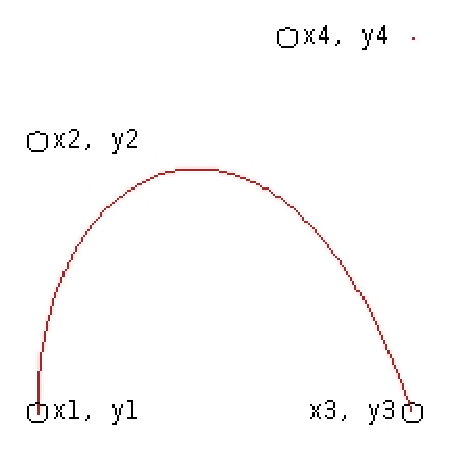
\includegraphics[width=\textwidth,height=\textheight/2,keepaspectratio=true]{images/curva_bezier}
\caption{Example output}
\end{DoxyImage}

\begin{DoxyParams}{Parameters}
{\em image} & Image where draw the curve \\
\hline
{\em x1} & Start coordinate x of the curve \\
\hline
{\em y1} & Start coordinate y of the curve \\
\hline
{\em x2} & First reference coordinate x \\
\hline
{\em y2} & First reference coordinate y \\
\hline
{\em x3} & End coordinate x of the curve \\
\hline
{\em y3} & End coordinate y of the curve \\
\hline
{\em x4} & Second reference coordinate x \\
\hline
{\em y4} & Second reference coordinate y \\
\hline
{\em \+\_\+p} & Number of steps to draw the curve, -\/1 to set default steps ( 1024 ) \\
\hline
{\em pixel} & Color and level of the curve \\
\hline
\end{DoxyParams}
\index{draw.\+c@{draw.\+c}!imel\+\_\+draw\+\_\+dashed\+\_\+grid@{imel\+\_\+draw\+\_\+dashed\+\_\+grid}}
\index{imel\+\_\+draw\+\_\+dashed\+\_\+grid@{imel\+\_\+draw\+\_\+dashed\+\_\+grid}!draw.\+c@{draw.\+c}}
\subsubsection[{\texorpdfstring{imel\+\_\+draw\+\_\+dashed\+\_\+grid(\+Imel\+Image $\ast$image, Imel\+Size sx, Imel\+Size sy, Imel\+Size ex, Imel\+Size ey, Imel\+Size col\+\_\+space, Imel\+Size row\+\_\+space, Imel\+Size size\+\_\+line, Imel\+Size space\+\_\+line, bool init\+\_\+from\+\_\+start, Imel\+Pixel pixel)}{imel_draw_dashed_grid(ImelImage *image, ImelSize sx, ImelSize sy, ImelSize ex, ImelSize ey, ImelSize col_space, ImelSize row_space, ImelSize size_line, ImelSize space_line, bool init_from_start, ImelPixel pixel)}}]{\setlength{\rightskip}{0pt plus 5cm}void imel\+\_\+draw\+\_\+dashed\+\_\+grid (
\begin{DoxyParamCaption}
\item[{{\bf Imel\+Image} $\ast$}]{image, }
\item[{{\bf Imel\+Size}}]{sx, }
\item[{{\bf Imel\+Size}}]{sy, }
\item[{{\bf Imel\+Size}}]{ex, }
\item[{{\bf Imel\+Size}}]{ey, }
\item[{{\bf Imel\+Size}}]{col\+\_\+space, }
\item[{{\bf Imel\+Size}}]{row\+\_\+space, }
\item[{{\bf Imel\+Size}}]{size\+\_\+line, }
\item[{{\bf Imel\+Size}}]{space\+\_\+line, }
\item[{{\bf bool}}]{init\+\_\+from\+\_\+start, }
\item[{{\bf Imel\+Pixel}}]{pixel}
\end{DoxyParamCaption}
)}\hypertarget{draw_8c_a95650481eb72e49f9a549d11927f9d21}{}\label{draw_8c_a95650481eb72e49f9a549d11927f9d21}


Draw a dashed grid. 

This function draw a dashed grid in {\ttfamily image} from coordinate $(sx,sy)$ to coordinate $(ex,ey)$ with columns length {\ttfamily col\+\_\+space} and rows length {\ttfamily row\+\_\+space}.


\begin{DoxyParams}{Parameters}
{\em image} & Image where draw the grid \\
\hline
{\em sx} & Start coordinate x of the grid \\
\hline
{\em sy} & Start coordinate y of the grid \\
\hline
{\em ex} & End coordinate x of the grid \\
\hline
{\em ey} & End coordinate y of the grid \\
\hline
{\em col\+\_\+space} & Space between columns \\
\hline
{\em row\+\_\+space} & Space between rows \\
\hline
{\em size\+\_\+line} & Length of the small lines \\
\hline
{\em space\+\_\+line} & Space between the small lines \\
\hline
{\em init\+\_\+from\+\_\+start} & T\+R\+UE if the first column and row init from coordinate $(sx,sy)$, else F\+A\+L\+SE \\
\hline
{\em pixel} & Color and level of the line \\
\hline
\end{DoxyParams}
\begin{DoxySeeAlso}{See also}
\hyperlink{draw_8c_a2864f976c426f7664dea01afff43f794}{imel\+\_\+draw\+\_\+dashed\+\_\+line} 
\end{DoxySeeAlso}
\index{draw.\+c@{draw.\+c}!imel\+\_\+draw\+\_\+dashed\+\_\+line@{imel\+\_\+draw\+\_\+dashed\+\_\+line}}
\index{imel\+\_\+draw\+\_\+dashed\+\_\+line@{imel\+\_\+draw\+\_\+dashed\+\_\+line}!draw.\+c@{draw.\+c}}
\subsubsection[{\texorpdfstring{imel\+\_\+draw\+\_\+dashed\+\_\+line(\+Imel\+Image $\ast$image, Imel\+Size \+\_\+x1, Imel\+Size \+\_\+y1, Imel\+Size \+\_\+x2, Imel\+Size \+\_\+y2, Imel\+Size size\+\_\+line, Imel\+Size space\+\_\+line, Imel\+Pixel pixel)}{imel_draw_dashed_line(ImelImage *image, ImelSize _x1, ImelSize _y1, ImelSize _x2, ImelSize _y2, ImelSize size_line, ImelSize space_line, ImelPixel pixel)}}]{\setlength{\rightskip}{0pt plus 5cm}{\bf bool} imel\+\_\+draw\+\_\+dashed\+\_\+line (
\begin{DoxyParamCaption}
\item[{{\bf Imel\+Image} $\ast$}]{image, }
\item[{{\bf Imel\+Size}}]{\+\_\+x1, }
\item[{{\bf Imel\+Size}}]{\+\_\+y1, }
\item[{{\bf Imel\+Size}}]{\+\_\+x2, }
\item[{{\bf Imel\+Size}}]{\+\_\+y2, }
\item[{{\bf Imel\+Size}}]{size\+\_\+line, }
\item[{{\bf Imel\+Size}}]{space\+\_\+line, }
\item[{{\bf Imel\+Pixel}}]{pixel}
\end{DoxyParamCaption}
)}\hypertarget{draw_8c_a2864f976c426f7664dea01afff43f794}{}\label{draw_8c_a2864f976c426f7664dea01afff43f794}


Draw a dashed line. 

This function draw a dashed line in {\ttfamily image} from coordinate $(\_x_1,\_y_1)$ to coordinate $(\_x_2,\_y_2)$ with small lines length {\ttfamily size\+\_\+line} pixels and space between them of {\ttfamily space\+\_\+line} pixels.


\begin{DoxyParams}{Parameters}
{\em image} & Image where draw the line \\
\hline
{\em \+\_\+x1} & Start coordinate x of the line \\
\hline
{\em \+\_\+y1} & Start coordinate y of the line \\
\hline
{\em \+\_\+x2} & End coordinate x of the line \\
\hline
{\em \+\_\+y2} & End coordinate y of the line \\
\hline
{\em size\+\_\+line} & Length of the small lines \\
\hline
{\em space\+\_\+line} & Space between the small lines \\
\hline
{\em pixel} & Color and level of the line \\
\hline
\end{DoxyParams}
\begin{DoxyReturn}{Returns}
F\+A\+L\+SE if image or size\+\_\+line values aren\textquotesingle{}t valid, else T\+R\+UE 
\end{DoxyReturn}
\index{draw.\+c@{draw.\+c}!imel\+\_\+draw\+\_\+ellipse@{imel\+\_\+draw\+\_\+ellipse}}
\index{imel\+\_\+draw\+\_\+ellipse@{imel\+\_\+draw\+\_\+ellipse}!draw.\+c@{draw.\+c}}
\subsubsection[{\texorpdfstring{imel\+\_\+draw\+\_\+ellipse(\+Imel\+Image $\ast$image, Imel\+Size x, Imel\+Size y, double a, double b, Imel\+Pixel pxl)}{imel_draw_ellipse(ImelImage *image, ImelSize x, ImelSize y, double a, double b, ImelPixel pxl)}}]{\setlength{\rightskip}{0pt plus 5cm}void imel\+\_\+draw\+\_\+ellipse (
\begin{DoxyParamCaption}
\item[{{\bf Imel\+Image} $\ast$}]{image, }
\item[{{\bf Imel\+Size}}]{x, }
\item[{{\bf Imel\+Size}}]{y, }
\item[{double}]{a, }
\item[{double}]{b, }
\item[{{\bf Imel\+Pixel}}]{pxl}
\end{DoxyParamCaption}
)}\hypertarget{draw_8c_a6e85b1251f6fe37a3fd75e2642ef7d10}{}\label{draw_8c_a6e85b1251f6fe37a3fd75e2642ef7d10}


Draw an ellipse. 

This function draw an ellipse in {\ttfamily image} with center in coordinate $(x,y)$ with {\ttfamily a} width and {\ttfamily b} height.


\begin{DoxyParams}{Parameters}
{\em image} & Image where draw the ellipse \\
\hline
{\em x} & Coordinate x of the ellipse center \\
\hline
{\em y} & Coordinate y of the ellipse center \\
\hline
{\em a} & Length of the horizontal axis \\
\hline
{\em b} & Length of the vertical axis \\
\hline
{\em pxl} & Color and level of the ellipse \\
\hline
\end{DoxyParams}
\index{draw.\+c@{draw.\+c}!imel\+\_\+draw\+\_\+figure@{imel\+\_\+draw\+\_\+figure}}
\index{imel\+\_\+draw\+\_\+figure@{imel\+\_\+draw\+\_\+figure}!draw.\+c@{draw.\+c}}
\subsubsection[{\texorpdfstring{imel\+\_\+draw\+\_\+figure(\+Imel\+Image $\ast$image, Imel\+Size n\+\_\+points, Imel\+Point $\ast$$\ast$starts, Imel\+Point $\ast$$\ast$ends, Imel\+Pixel pixel)}{imel_draw_figure(ImelImage *image, ImelSize n_points, ImelPoint **starts, ImelPoint **ends, ImelPixel pixel)}}]{\setlength{\rightskip}{0pt plus 5cm}void imel\+\_\+draw\+\_\+figure (
\begin{DoxyParamCaption}
\item[{{\bf Imel\+Image} $\ast$}]{image, }
\item[{{\bf Imel\+Size}}]{n\+\_\+points, }
\item[{{\bf Imel\+Point} $\ast$$\ast$}]{starts, }
\item[{{\bf Imel\+Point} $\ast$$\ast$}]{ends, }
\item[{{\bf Imel\+Pixel}}]{pixel}
\end{DoxyParamCaption}
)}\hypertarget{draw_8c_a2269fedea0f39513774d343c09587f2a}{}\label{draw_8c_a2269fedea0f39513774d343c09587f2a}


Draw a non contiguous figure. 

This function draw a non contiguous figure in {\ttfamily image} where each start and end point is knowed. Each point have color and level passed {\ttfamily pixel} 


\begin{DoxyCode}
1 ImelPoint *starts[4] = \{ NULL \}, *ends[3];
2 ImelPixel pixel = \{ 255, 0, 0, 0 \};
3 
4 image = imel\_image\_new (64, 64);
5 
6 starts[0] = imel\_point\_new (image, 8, 8, pixel);
7 starts[1] = imel\_point\_new (image, 56, 8, pixel);
8 starts[2] = imel\_point\_new (image, 32, 58, pixel);
9 
10 ends[0] = imel\_point\_new (image, 32, 32, pixel);
11 ends[1] = ends[2] = ends[0];
12 
13 imel\_draw\_figure (image, 3, starts, ends, pixel);
14 imel\_point\_free (ends[0]);
15 imel\_point\_array\_free (starts);
\end{DoxyCode}
 
\begin{DoxyImage}

\includegraphics[width=\textwidth,height=\textheight/2,keepaspectratio=true]{images/draw_figure}
\caption{Example output}
\end{DoxyImage}

\begin{DoxyParams}{Parameters}
{\em image} & Image where draw the figure \\
\hline
{\em n\+\_\+points} & Number of points in {\ttfamily starts} and {\ttfamily ends} \\
\hline
{\em starts} & Start points \\
\hline
{\em ends} & End points \\
\hline
{\em pixel} & Color and level of the figure \\
\hline
\end{DoxyParams}
\index{draw.\+c@{draw.\+c}!imel\+\_\+draw\+\_\+filled\+\_\+arch@{imel\+\_\+draw\+\_\+filled\+\_\+arch}}
\index{imel\+\_\+draw\+\_\+filled\+\_\+arch@{imel\+\_\+draw\+\_\+filled\+\_\+arch}!draw.\+c@{draw.\+c}}
\subsubsection[{\texorpdfstring{imel\+\_\+draw\+\_\+filled\+\_\+arch(\+Imel\+Image $\ast$image, Imel\+Size x, Imel\+Size y, Imel\+Size radius, double start\+\_\+angle, double end\+\_\+angle, Imel\+Pixel pxl)}{imel_draw_filled_arch(ImelImage *image, ImelSize x, ImelSize y, ImelSize radius, double start_angle, double end_angle, ImelPixel pxl)}}]{\setlength{\rightskip}{0pt plus 5cm}{\bf bool} imel\+\_\+draw\+\_\+filled\+\_\+arch (
\begin{DoxyParamCaption}
\item[{{\bf Imel\+Image} $\ast$}]{image, }
\item[{{\bf Imel\+Size}}]{x, }
\item[{{\bf Imel\+Size}}]{y, }
\item[{{\bf Imel\+Size}}]{radius, }
\item[{double}]{start\+\_\+angle, }
\item[{double}]{end\+\_\+angle, }
\item[{{\bf Imel\+Pixel}}]{pxl}
\end{DoxyParamCaption}
)}\hypertarget{draw_8c_ac7a6615ed3eeda8f99766116040a86e9}{}\label{draw_8c_ac7a6615ed3eeda8f99766116040a86e9}


Draw a filled arch. 

This function draw a filled arch in {\ttfamily image} with center in coordinate $(x,y)$ and radius of {\ttfamily radius} pixels.


\begin{DoxyParams}{Parameters}
{\em image} & Image where draw the arch \\
\hline
{\em x} & Center coordinate x \\
\hline
{\em y} & Center coordinate y \\
\hline
{\em radius} & Radius of the arch \\
\hline
{\em start\+\_\+angle} & Start angle of the arch in radians \\
\hline
{\em end\+\_\+angle} & End angle of the arch in radians \\
\hline
{\em pxl} & Color and level of the arch \\
\hline
\end{DoxyParams}
\begin{DoxyReturn}{Returns}
T\+R\+UE if all values are valid, else F\+A\+L\+SE 
\end{DoxyReturn}
\begin{DoxySeeAlso}{See also}
\hyperlink{draw_8c_a4cc27abce5f2d1cfe72dc7e5b078adc8}{imel\+\_\+draw\+\_\+arch} 
\end{DoxySeeAlso}
\index{draw.\+c@{draw.\+c}!imel\+\_\+draw\+\_\+filled\+\_\+circle@{imel\+\_\+draw\+\_\+filled\+\_\+circle}}
\index{imel\+\_\+draw\+\_\+filled\+\_\+circle@{imel\+\_\+draw\+\_\+filled\+\_\+circle}!draw.\+c@{draw.\+c}}
\subsubsection[{\texorpdfstring{imel\+\_\+draw\+\_\+filled\+\_\+circle(\+Imel\+Image $\ast$image, Imel\+Size x, Imel\+Size y, Imel\+Size radius, Imel\+Pixel pxl)}{imel_draw_filled_circle(ImelImage *image, ImelSize x, ImelSize y, ImelSize radius, ImelPixel pxl)}}]{\setlength{\rightskip}{0pt plus 5cm}void imel\+\_\+draw\+\_\+filled\+\_\+circle (
\begin{DoxyParamCaption}
\item[{{\bf Imel\+Image} $\ast$}]{image, }
\item[{{\bf Imel\+Size}}]{x, }
\item[{{\bf Imel\+Size}}]{y, }
\item[{{\bf Imel\+Size}}]{radius, }
\item[{{\bf Imel\+Pixel}}]{pxl}
\end{DoxyParamCaption}
)}\hypertarget{draw_8c_a9d6234ac96cccab2e2d6b36acc78a865}{}\label{draw_8c_a9d6234ac96cccab2e2d6b36acc78a865}


Draw a filled circle. 

This function draw a circle filled with color and level passed in {\ttfamily pxl} at coordinate $(x,y)$ with a radius of {\ttfamily radius} pixels.


\begin{DoxyParams}{Parameters}
{\em image} & Image where draw the circle \\
\hline
{\em x} & Coordinate x of the circle center \\
\hline
{\em y} & Coordinate y of the circle center \\
\hline
{\em radius} & Radius of the circle in pixels \\
\hline
{\em pxl} & Color and level of the circle \\
\hline
\end{DoxyParams}
\index{draw.\+c@{draw.\+c}!imel\+\_\+draw\+\_\+filled\+\_\+ellipse@{imel\+\_\+draw\+\_\+filled\+\_\+ellipse}}
\index{imel\+\_\+draw\+\_\+filled\+\_\+ellipse@{imel\+\_\+draw\+\_\+filled\+\_\+ellipse}!draw.\+c@{draw.\+c}}
\subsubsection[{\texorpdfstring{imel\+\_\+draw\+\_\+filled\+\_\+ellipse(\+Imel\+Image $\ast$image, Imel\+Size x, Imel\+Size y, double a, double b, Imel\+Pixel pxl)}{imel_draw_filled_ellipse(ImelImage *image, ImelSize x, ImelSize y, double a, double b, ImelPixel pxl)}}]{\setlength{\rightskip}{0pt plus 5cm}void imel\+\_\+draw\+\_\+filled\+\_\+ellipse (
\begin{DoxyParamCaption}
\item[{{\bf Imel\+Image} $\ast$}]{image, }
\item[{{\bf Imel\+Size}}]{x, }
\item[{{\bf Imel\+Size}}]{y, }
\item[{double}]{a, }
\item[{double}]{b, }
\item[{{\bf Imel\+Pixel}}]{pxl}
\end{DoxyParamCaption}
)}\hypertarget{draw_8c_a9e9f3690fd2cb70848b39036a1fe9745}{}\label{draw_8c_a9e9f3690fd2cb70848b39036a1fe9745}


Draw a filled ellipse. 

This function draw a filled ellipse in {\ttfamily image} with center in coordinate $(x,y)$ with {\ttfamily a} width and {\ttfamily b} height.


\begin{DoxyParams}{Parameters}
{\em image} & Image where draw the ellipse \\
\hline
{\em x} & Coordinate x of the ellipse center \\
\hline
{\em y} & Coordinate y of the ellipse center \\
\hline
{\em a} & Length of the horizontal axis \\
\hline
{\em b} & Length of the vertical axis \\
\hline
{\em pxl} & Color and level of the ellipse \\
\hline
\end{DoxyParams}
\index{draw.\+c@{draw.\+c}!imel\+\_\+draw\+\_\+filled\+\_\+line@{imel\+\_\+draw\+\_\+filled\+\_\+line}}
\index{imel\+\_\+draw\+\_\+filled\+\_\+line@{imel\+\_\+draw\+\_\+filled\+\_\+line}!draw.\+c@{draw.\+c}}
\subsubsection[{\texorpdfstring{imel\+\_\+draw\+\_\+filled\+\_\+line(\+Imel\+Image $\ast$image, Imel\+Size \+\_\+x1, Imel\+Size \+\_\+y1, Imel\+Size \+\_\+x2, Imel\+Size \+\_\+y2, Imel\+Size ox, Imel\+Size oy, Imel\+Pixel pixel)}{imel_draw_filled_line(ImelImage *image, ImelSize _x1, ImelSize _y1, ImelSize _x2, ImelSize _y2, ImelSize ox, ImelSize oy, ImelPixel pixel)}}]{\setlength{\rightskip}{0pt plus 5cm}{\bf bool} imel\+\_\+draw\+\_\+filled\+\_\+line (
\begin{DoxyParamCaption}
\item[{{\bf Imel\+Image} $\ast$}]{image, }
\item[{{\bf Imel\+Size}}]{\+\_\+x1, }
\item[{{\bf Imel\+Size}}]{\+\_\+y1, }
\item[{{\bf Imel\+Size}}]{\+\_\+x2, }
\item[{{\bf Imel\+Size}}]{\+\_\+y2, }
\item[{{\bf Imel\+Size}}]{ox, }
\item[{{\bf Imel\+Size}}]{oy, }
\item[{{\bf Imel\+Pixel}}]{pixel}
\end{DoxyParamCaption}
)}\hypertarget{draw_8c_a538f52427d2d8f84b45e5570d1dbf080}{}\label{draw_8c_a538f52427d2d8f84b45e5570d1dbf080}


Draw a filled line. 

This function draw a line in {\ttfamily image} from coordinate $(\_x_1,\_y_1)$ to coordinate $(\_x_2,\_y_2)$ with a color and level passed in {\ttfamily pixel}, where each point of the line is linked to a coordinate $(ox,oy)$.


\begin{DoxyParams}{Parameters}
{\em image} & Image where draw the line \\
\hline
{\em \+\_\+x1} & Start x coordinate \\
\hline
{\em \+\_\+y1} & Start y coordinate \\
\hline
{\em \+\_\+x2} & End x coordinate \\
\hline
{\em \+\_\+y2} & End y coordinate \\
\hline
{\em ox} & Coordinate x of the common point \\
\hline
{\em oy} & Coordinate y of the common point \\
\hline
{\em pixel} & Color and level of the line \\
\hline
\end{DoxyParams}
\begin{DoxyReturn}{Returns}
F\+A\+L\+SE if {\ttfamily image} isn\textquotesingle{}t a valid image, else T\+R\+UE 
\end{DoxyReturn}
\index{draw.\+c@{draw.\+c}!imel\+\_\+draw\+\_\+gradient@{imel\+\_\+draw\+\_\+gradient}}
\index{imel\+\_\+draw\+\_\+gradient@{imel\+\_\+draw\+\_\+gradient}!draw.\+c@{draw.\+c}}
\subsubsection[{\texorpdfstring{imel\+\_\+draw\+\_\+gradient(\+Imel\+Image $\ast$image, Imel\+Orientation orientation, Imel\+Size start, Imel\+Size end, Imel\+Pixel start\+\_\+color, Imel\+Pixel end\+\_\+color)}{imel_draw_gradient(ImelImage *image, ImelOrientation orientation, ImelSize start, ImelSize end, ImelPixel start_color, ImelPixel end_color)}}]{\setlength{\rightskip}{0pt plus 5cm}void imel\+\_\+draw\+\_\+gradient (
\begin{DoxyParamCaption}
\item[{{\bf Imel\+Image} $\ast$}]{image, }
\item[{{\bf Imel\+Orientation}}]{orientation, }
\item[{{\bf Imel\+Size}}]{start, }
\item[{{\bf Imel\+Size}}]{end, }
\item[{{\bf Imel\+Pixel}}]{start\+\_\+color, }
\item[{{\bf Imel\+Pixel}}]{end\+\_\+color}
\end{DoxyParamCaption}
)}\hypertarget{draw_8c_a94c27538a3f6dec9bbd8b8790e37d08f}{}\label{draw_8c_a94c27538a3f6dec9bbd8b8790e37d08f}


Draw a gradient. 

This function draw a gradient in {\ttfamily image}, with an {\ttfamily orientation} chosen, from color and level passed in {\ttfamily start\+\_\+color} to {\ttfamily end\+\_\+color}.


\begin{DoxyParams}{Parameters}
{\em image} & Image where draw the gradient \\
\hline
{\em orientation} & Gradient orientation \\
\hline
{\em start} & Start row or column ( depends from orientation ) \\
\hline
{\em end} & End row or column ( depends from orientation ) \\
\hline
{\em start\+\_\+color} & Start color and level \\
\hline
{\em end\+\_\+color} & End color and level \\
\hline
\end{DoxyParams}
\index{draw.\+c@{draw.\+c}!imel\+\_\+draw\+\_\+gradient\+\_\+curve@{imel\+\_\+draw\+\_\+gradient\+\_\+curve}}
\index{imel\+\_\+draw\+\_\+gradient\+\_\+curve@{imel\+\_\+draw\+\_\+gradient\+\_\+curve}!draw.\+c@{draw.\+c}}
\subsubsection[{\texorpdfstring{imel\+\_\+draw\+\_\+gradient\+\_\+curve(\+Imel\+Image $\ast$image, Imel\+Size x1, Imel\+Size y1, Imel\+Size x2, Imel\+Size y2, Imel\+Size x3, Imel\+Size y3, Imel\+Size x4, Imel\+Size y4, int \+\_\+p, Imel\+Pixel start, Imel\+Pixel end)}{imel_draw_gradient_curve(ImelImage *image, ImelSize x1, ImelSize y1, ImelSize x2, ImelSize y2, ImelSize x3, ImelSize y3, ImelSize x4, ImelSize y4, int _p, ImelPixel start, ImelPixel end)}}]{\setlength{\rightskip}{0pt plus 5cm}void imel\+\_\+draw\+\_\+gradient\+\_\+curve (
\begin{DoxyParamCaption}
\item[{{\bf Imel\+Image} $\ast$}]{image, }
\item[{{\bf Imel\+Size}}]{x1, }
\item[{{\bf Imel\+Size}}]{y1, }
\item[{{\bf Imel\+Size}}]{x2, }
\item[{{\bf Imel\+Size}}]{y2, }
\item[{{\bf Imel\+Size}}]{x3, }
\item[{{\bf Imel\+Size}}]{y3, }
\item[{{\bf Imel\+Size}}]{x4, }
\item[{{\bf Imel\+Size}}]{y4, }
\item[{int}]{\+\_\+p, }
\item[{{\bf Imel\+Pixel}}]{start, }
\item[{{\bf Imel\+Pixel}}]{end}
\end{DoxyParamCaption}
)}\hypertarget{draw_8c_ae51d3cb0d3e8009f633d4943f8ce53fa}{}\label{draw_8c_ae51d3cb0d3e8009f633d4943f8ce53fa}


Draw a Bèzier\textquotesingle{}s curve with gradient. 

This function draw a Bèzier\textquotesingle{}s curve in {\ttfamily image} with gradient from color and level passed in {\ttfamily start} to color and level passed in {\ttfamily end}.


\begin{DoxyParams}{Parameters}
{\em image} & Image where draw the curve \\
\hline
{\em x1} & Start coordinate x of the curve \\
\hline
{\em y1} & Start coordinate y of the curve \\
\hline
{\em x2} & First reference coordinate x \\
\hline
{\em y2} & First reference coordinate y \\
\hline
{\em x3} & End coordinate x of the curve \\
\hline
{\em y3} & End coordinate y of the curve \\
\hline
{\em x4} & Second reference coordinate x \\
\hline
{\em y4} & Second reference coordinate y \\
\hline
{\em \+\_\+p} & Number of steps to draw the curve, -\/1 to set default steps ( 1024 ) \\
\hline
{\em start} & Start color and level of the curve \\
\hline
{\em end} & End color and level of the curve \\
\hline
\end{DoxyParams}
\begin{DoxySeeAlso}{See also}
\hyperlink{draw_8c_afa90031c54946a102a04d37f86053605}{imel\+\_\+draw\+\_\+curve} 
\end{DoxySeeAlso}
\index{draw.\+c@{draw.\+c}!imel\+\_\+draw\+\_\+gradient\+\_\+line@{imel\+\_\+draw\+\_\+gradient\+\_\+line}}
\index{imel\+\_\+draw\+\_\+gradient\+\_\+line@{imel\+\_\+draw\+\_\+gradient\+\_\+line}!draw.\+c@{draw.\+c}}
\subsubsection[{\texorpdfstring{imel\+\_\+draw\+\_\+gradient\+\_\+line(\+Imel\+Image $\ast$image, Imel\+Size \+\_\+x1, Imel\+Size \+\_\+y1, Imel\+Size \+\_\+x2, Imel\+Size \+\_\+y2, Imel\+Pixel start, Imel\+Pixel end)}{imel_draw_gradient_line(ImelImage *image, ImelSize _x1, ImelSize _y1, ImelSize _x2, ImelSize _y2, ImelPixel start, ImelPixel end)}}]{\setlength{\rightskip}{0pt plus 5cm}{\bf bool} imel\+\_\+draw\+\_\+gradient\+\_\+line (
\begin{DoxyParamCaption}
\item[{{\bf Imel\+Image} $\ast$}]{image, }
\item[{{\bf Imel\+Size}}]{\+\_\+x1, }
\item[{{\bf Imel\+Size}}]{\+\_\+y1, }
\item[{{\bf Imel\+Size}}]{\+\_\+x2, }
\item[{{\bf Imel\+Size}}]{\+\_\+y2, }
\item[{{\bf Imel\+Pixel}}]{start, }
\item[{{\bf Imel\+Pixel}}]{end}
\end{DoxyParamCaption}
)}\hypertarget{draw_8c_a0f17ca4ca8df8aada79f12e7cbd2397b}{}\label{draw_8c_a0f17ca4ca8df8aada79f12e7cbd2397b}


Draw a line with gradient. 

This function draw a line in {\ttfamily image} from coordinate $(\_x_1,\_y_1)$ to coordinate $(\_x_2,\_y_2)$ with a color and level gradient from {\ttfamily start} to {\ttfamily end}.


\begin{DoxyParams}{Parameters}
{\em image} & Image where draw the line \\
\hline
{\em \+\_\+x1} & Start x coordinate \\
\hline
{\em \+\_\+y1} & Start y coordinate \\
\hline
{\em \+\_\+x2} & End x coordinate \\
\hline
{\em \+\_\+y2} & End y coordinate \\
\hline
{\em start} & Start color and level of the line \\
\hline
{\em end} & End color and level of the line \\
\hline
\end{DoxyParams}
\begin{DoxyReturn}{Returns}
F\+A\+L\+SE if {\ttfamily image} isn\textquotesingle{}t a valid image, else T\+R\+UE 
\end{DoxyReturn}
\begin{DoxySeeAlso}{See also}
\hyperlink{draw_8c_a0168dd78ad67c50479e3244c9f6cc2a6}{imel\+\_\+draw\+\_\+line} 
\end{DoxySeeAlso}
\index{draw.\+c@{draw.\+c}!imel\+\_\+draw\+\_\+grid@{imel\+\_\+draw\+\_\+grid}}
\index{imel\+\_\+draw\+\_\+grid@{imel\+\_\+draw\+\_\+grid}!draw.\+c@{draw.\+c}}
\subsubsection[{\texorpdfstring{imel\+\_\+draw\+\_\+grid(\+Imel\+Image $\ast$image, Imel\+Size sx, Imel\+Size sy, Imel\+Size ex, Imel\+Size ey, Imel\+Size col\+\_\+space, Imel\+Size row\+\_\+space, bool init\+\_\+from\+\_\+start, Imel\+Pixel pixel)}{imel_draw_grid(ImelImage *image, ImelSize sx, ImelSize sy, ImelSize ex, ImelSize ey, ImelSize col_space, ImelSize row_space, bool init_from_start, ImelPixel pixel)}}]{\setlength{\rightskip}{0pt plus 5cm}void imel\+\_\+draw\+\_\+grid (
\begin{DoxyParamCaption}
\item[{{\bf Imel\+Image} $\ast$}]{image, }
\item[{{\bf Imel\+Size}}]{sx, }
\item[{{\bf Imel\+Size}}]{sy, }
\item[{{\bf Imel\+Size}}]{ex, }
\item[{{\bf Imel\+Size}}]{ey, }
\item[{{\bf Imel\+Size}}]{col\+\_\+space, }
\item[{{\bf Imel\+Size}}]{row\+\_\+space, }
\item[{{\bf bool}}]{init\+\_\+from\+\_\+start, }
\item[{{\bf Imel\+Pixel}}]{pixel}
\end{DoxyParamCaption}
)}\hypertarget{draw_8c_a57f5caaec1f269da475429df204d4829}{}\label{draw_8c_a57f5caaec1f269da475429df204d4829}


Draw a grid. 

This function draw a grid in {\ttfamily image} from coordinate $(sx,sy)$ to coordinate $(ex,ey)$ witch columns length {\ttfamily col\+\_\+space} and rows length {\ttfamily row\+\_\+space}.


\begin{DoxyParams}{Parameters}
{\em image} & Image where draw the grid \\
\hline
{\em sx} & Start coordinate x of the grid \\
\hline
{\em sy} & Start coordinate y of the grid \\
\hline
{\em ex} & End coordinate x of the grid \\
\hline
{\em ey} & End coordinate y of the grid \\
\hline
{\em col\+\_\+space} & Space between columns \\
\hline
{\em row\+\_\+space} & Space between rows \\
\hline
{\em init\+\_\+from\+\_\+start} & T\+R\+UE if the first column and row init from coordinate $(sx,sy)$, else F\+A\+L\+SE \\
\hline
{\em pixel} & Color and level of the line \\
\hline
\end{DoxyParams}
\index{draw.\+c@{draw.\+c}!imel\+\_\+draw\+\_\+line@{imel\+\_\+draw\+\_\+line}}
\index{imel\+\_\+draw\+\_\+line@{imel\+\_\+draw\+\_\+line}!draw.\+c@{draw.\+c}}
\subsubsection[{\texorpdfstring{imel\+\_\+draw\+\_\+line(\+Imel\+Image $\ast$image, Imel\+Size \+\_\+sx, Imel\+Size \+\_\+sy, Imel\+Size \+\_\+ex, Imel\+Size \+\_\+ey, Imel\+Pixel pixel)}{imel_draw_line(ImelImage *image, ImelSize _sx, ImelSize _sy, ImelSize _ex, ImelSize _ey, ImelPixel pixel)}}]{\setlength{\rightskip}{0pt plus 5cm}{\bf bool} imel\+\_\+draw\+\_\+line (
\begin{DoxyParamCaption}
\item[{{\bf Imel\+Image} $\ast$}]{image, }
\item[{{\bf Imel\+Size}}]{\+\_\+sx, }
\item[{{\bf Imel\+Size}}]{\+\_\+sy, }
\item[{{\bf Imel\+Size}}]{\+\_\+ex, }
\item[{{\bf Imel\+Size}}]{\+\_\+ey, }
\item[{{\bf Imel\+Pixel}}]{pixel}
\end{DoxyParamCaption}
)}\hypertarget{draw_8c_a0168dd78ad67c50479e3244c9f6cc2a6}{}\label{draw_8c_a0168dd78ad67c50479e3244c9f6cc2a6}


Draw a line. 

This function draw a line in {\ttfamily image} from coordinate $(\_sx,\_sy)$ to coordinate $(\_ex,\_ey)$ with a color and level passed in {\ttfamily pixel} 


\begin{DoxyParams}{Parameters}
{\em image} & Image where draw the line \\
\hline
{\em \+\_\+sx} & Start x coordinate \\
\hline
{\em \+\_\+sy} & Start y coordinate \\
\hline
{\em \+\_\+ex} & End x coordinate \\
\hline
{\em \+\_\+ey} & End y coordinate \\
\hline
{\em pixel} & Color and level of the line \\
\hline
\end{DoxyParams}
\begin{DoxyReturn}{Returns}
F\+A\+L\+SE if {\ttfamily image} isn\textquotesingle{}t a valid image, else T\+R\+UE 
\end{DoxyReturn}
\index{draw.\+c@{draw.\+c}!imel\+\_\+draw\+\_\+line\+\_\+connecting\+\_\+all\+\_\+points@{imel\+\_\+draw\+\_\+line\+\_\+connecting\+\_\+all\+\_\+points}}
\index{imel\+\_\+draw\+\_\+line\+\_\+connecting\+\_\+all\+\_\+points@{imel\+\_\+draw\+\_\+line\+\_\+connecting\+\_\+all\+\_\+points}!draw.\+c@{draw.\+c}}
\subsubsection[{\texorpdfstring{imel\+\_\+draw\+\_\+line\+\_\+connecting\+\_\+all\+\_\+points(\+Imel\+Image $\ast$image, Imel\+Point $\ast$$\ast$points, Imel\+Pixel pxl)}{imel_draw_line_connecting_all_points(ImelImage *image, ImelPoint **points, ImelPixel pxl)}}]{\setlength{\rightskip}{0pt plus 5cm}void imel\+\_\+draw\+\_\+line\+\_\+connecting\+\_\+all\+\_\+points (
\begin{DoxyParamCaption}
\item[{{\bf Imel\+Image} $\ast$}]{image, }
\item[{{\bf Imel\+Point} $\ast$$\ast$}]{points, }
\item[{{\bf Imel\+Pixel}}]{pxl}
\end{DoxyParamCaption}
)}\hypertarget{draw_8c_a952856ed6ab73528312b3be16b5d2f67}{}\label{draw_8c_a952856ed6ab73528312b3be16b5d2f67}


Draw lines between all points passed. 

This function draw lines from each point to all different points linking each one to all others.


\begin{DoxyParams}{Parameters}
{\em image} & Image where draw these lines \\
\hline
{\em points} & A N\+U\+L\+L-\/terminated array with the points to link \\
\hline
{\em pxl} & Color and level of the lines \\
\hline
\end{DoxyParams}
\index{draw.\+c@{draw.\+c}!imel\+\_\+draw\+\_\+partial\+\_\+reg\+\_\+shape@{imel\+\_\+draw\+\_\+partial\+\_\+reg\+\_\+shape}}
\index{imel\+\_\+draw\+\_\+partial\+\_\+reg\+\_\+shape@{imel\+\_\+draw\+\_\+partial\+\_\+reg\+\_\+shape}!draw.\+c@{draw.\+c}}
\subsubsection[{\texorpdfstring{imel\+\_\+draw\+\_\+partial\+\_\+reg\+\_\+shape(\+Imel\+Image $\ast$image, Imel\+Size x, Imel\+Size y, Imel\+Size r, long v, short p, double start\+\_\+angle, Imel\+Pixel pxl)}{imel_draw_partial_reg_shape(ImelImage *image, ImelSize x, ImelSize y, ImelSize r, long v, short p, double start_angle, ImelPixel pxl)}}]{\setlength{\rightskip}{0pt plus 5cm}{\bf bool} imel\+\_\+draw\+\_\+partial\+\_\+reg\+\_\+shape (
\begin{DoxyParamCaption}
\item[{{\bf Imel\+Image} $\ast$}]{image, }
\item[{{\bf Imel\+Size}}]{x, }
\item[{{\bf Imel\+Size}}]{y, }
\item[{{\bf Imel\+Size}}]{r, }
\item[{long}]{v, }
\item[{short}]{p, }
\item[{double}]{start\+\_\+angle, }
\item[{{\bf Imel\+Pixel}}]{pxl}
\end{DoxyParamCaption}
)}\hypertarget{draw_8c_ad8b931ece29f161af9b5a4153d186dd4}{}\label{draw_8c_ad8b931ece29f161af9b5a4153d186dd4}


Draw a partial regular shape. 

This function draw a partial regular shape in {\ttfamily image} with center in coordinate $(x,y)$, radius {\ttfamily r}, vertices {\ttfamily v} and rotation {\ttfamily start\+\_\+angle} in radians. The shape will be draw for only the {\ttfamily p} percent.


\begin{DoxyParams}{Parameters}
{\em image} & Image where draw the shape \\
\hline
{\em x} & Center coordinate x \\
\hline
{\em y} & Center coordinate y \\
\hline
{\em r} & Radius of the shape \\
\hline
{\em v} & Number of vertices \\
\hline
{\em p} & Percentage of the shape ( Values from 0 to 100 ) \\
\hline
{\em start\+\_\+angle} & Rotation angle in radians \\
\hline
{\em pxl} & Color and level of the shape \\
\hline
\end{DoxyParams}
\begin{DoxyReturn}{Returns}
T\+R\+UE if all values are valid, else F\+A\+L\+SE 
\end{DoxyReturn}
\begin{DoxySeeAlso}{See also}
\hyperlink{draw_8c_a15536050acc27defca08e29c54c6748e}{imel\+\_\+draw\+\_\+reg\+\_\+shape} 
\end{DoxySeeAlso}
\index{draw.\+c@{draw.\+c}!imel\+\_\+draw\+\_\+point@{imel\+\_\+draw\+\_\+point}}
\index{imel\+\_\+draw\+\_\+point@{imel\+\_\+draw\+\_\+point}!draw.\+c@{draw.\+c}}
\subsubsection[{\texorpdfstring{imel\+\_\+draw\+\_\+point(\+Imel\+Image $\ast$image, Imel\+Size x, Imel\+Size y, Imel\+Pixel pixel)}{imel_draw_point(ImelImage *image, ImelSize x, ImelSize y, ImelPixel pixel)}}]{\setlength{\rightskip}{0pt plus 5cm}void imel\+\_\+draw\+\_\+point (
\begin{DoxyParamCaption}
\item[{{\bf Imel\+Image} $\ast$}]{image, }
\item[{{\bf Imel\+Size}}]{x, }
\item[{{\bf Imel\+Size}}]{y, }
\item[{{\bf Imel\+Pixel}}]{pixel}
\end{DoxyParamCaption}
)}\hypertarget{draw_8c_a80e6d667aceb3de202823e5493a774b1}{}\label{draw_8c_a80e6d667aceb3de202823e5493a774b1}


Draw a single point in an image. 

This function draw a point in {\ttfamily image} at coordinate $(x,y)$ with color and level specified in {\ttfamily pixel}.


\begin{DoxyParams}{Parameters}
{\em image} & Image where draw the point \\
\hline
{\em x} & Coordinate x of the point \\
\hline
{\em y} & Coordinate y of the point \\
\hline
{\em pixel} & Color and level of the point \\
\hline
\end{DoxyParams}
\index{draw.\+c@{draw.\+c}!imel\+\_\+draw\+\_\+point\+\_\+from\+\_\+array@{imel\+\_\+draw\+\_\+point\+\_\+from\+\_\+array}}
\index{imel\+\_\+draw\+\_\+point\+\_\+from\+\_\+array@{imel\+\_\+draw\+\_\+point\+\_\+from\+\_\+array}!draw.\+c@{draw.\+c}}
\subsubsection[{\texorpdfstring{imel\+\_\+draw\+\_\+point\+\_\+from\+\_\+array(\+Imel\+Image $\ast$image, Imel\+Size n\+\_\+points, Imel\+Point $\ast$$\ast$points)}{imel_draw_point_from_array(ImelImage *image, ImelSize n_points, ImelPoint **points)}}]{\setlength{\rightskip}{0pt plus 5cm}void imel\+\_\+draw\+\_\+point\+\_\+from\+\_\+array (
\begin{DoxyParamCaption}
\item[{{\bf Imel\+Image} $\ast$}]{image, }
\item[{{\bf Imel\+Size}}]{n\+\_\+points, }
\item[{{\bf Imel\+Point} $\ast$$\ast$}]{points}
\end{DoxyParamCaption}
)}\hypertarget{draw_8c_a0f6a2052074967fa5b57e487544f42ee}{}\label{draw_8c_a0f6a2052074967fa5b57e487544f42ee}


Draw more point at the same time. 

This function draw a list of {\ttfamily points} in the {\ttfamily image} 


\begin{DoxyParams}{Parameters}
{\em image} & Image where draw the points \\
\hline
{\em n\+\_\+points} & Number of points to draw or 0 if {\ttfamily points} is a N\+U\+L\+L-\/terminated array and you want to draw its all. \\
\hline
{\em points} & Points to draw \\
\hline
\end{DoxyParams}
\index{draw.\+c@{draw.\+c}!imel\+\_\+draw\+\_\+rect@{imel\+\_\+draw\+\_\+rect}}
\index{imel\+\_\+draw\+\_\+rect@{imel\+\_\+draw\+\_\+rect}!draw.\+c@{draw.\+c}}
\subsubsection[{\texorpdfstring{imel\+\_\+draw\+\_\+rect(\+Imel\+Image $\ast$image, Imel\+Size x1, Imel\+Size y1, Imel\+Size x2, Imel\+Size y2, Imel\+Pixel pixel, bool fill)}{imel_draw_rect(ImelImage *image, ImelSize x1, ImelSize y1, ImelSize x2, ImelSize y2, ImelPixel pixel, bool fill)}}]{\setlength{\rightskip}{0pt plus 5cm}void imel\+\_\+draw\+\_\+rect (
\begin{DoxyParamCaption}
\item[{{\bf Imel\+Image} $\ast$}]{image, }
\item[{{\bf Imel\+Size}}]{x1, }
\item[{{\bf Imel\+Size}}]{y1, }
\item[{{\bf Imel\+Size}}]{x2, }
\item[{{\bf Imel\+Size}}]{y2, }
\item[{{\bf Imel\+Pixel}}]{pixel, }
\item[{{\bf bool}}]{fill}
\end{DoxyParamCaption}
)}\hypertarget{draw_8c_aa6c826f436252a630b7e4d1d10c73309}{}\label{draw_8c_aa6c826f436252a630b7e4d1d10c73309}


Draw a rectangle ( filled or not ) 

This function draw a rectangle that can be filled inside an {\ttfamily image} from coordinate $(x_1,y_1)$ to coordinate $(x_2,y_2)$ with color and level passed in {\ttfamily pixel}.


\begin{DoxyParams}{Parameters}
{\em image} & Image where draw the rectangle \\
\hline
{\em x1} & Start x coordinate of the rectangle \\
\hline
{\em y1} & Start y coordinate of the rectangle \\
\hline
{\em x2} & End x coordinate of the rectangle \\
\hline
{\em y2} & End y coordinate of the rectangle \\
\hline
{\em pixel} & Color and level of the rectangle \\
\hline
{\em fill} & T\+R\+UE for filled rectangle, else F\+A\+L\+SE \\
\hline
\end{DoxyParams}
\index{draw.\+c@{draw.\+c}!imel\+\_\+draw\+\_\+rect\+\_\+with\+\_\+rounded\+\_\+angles@{imel\+\_\+draw\+\_\+rect\+\_\+with\+\_\+rounded\+\_\+angles}}
\index{imel\+\_\+draw\+\_\+rect\+\_\+with\+\_\+rounded\+\_\+angles@{imel\+\_\+draw\+\_\+rect\+\_\+with\+\_\+rounded\+\_\+angles}!draw.\+c@{draw.\+c}}
\subsubsection[{\texorpdfstring{imel\+\_\+draw\+\_\+rect\+\_\+with\+\_\+rounded\+\_\+angles(\+Imel\+Image $\ast$image, Imel\+Size x1, Imel\+Size y1, Imel\+Size x2, Imel\+Size y2, Imel\+Size radius, Imel\+Pixel pixel, bool fill)}{imel_draw_rect_with_rounded_angles(ImelImage *image, ImelSize x1, ImelSize y1, ImelSize x2, ImelSize y2, ImelSize radius, ImelPixel pixel, bool fill)}}]{\setlength{\rightskip}{0pt plus 5cm}{\bf bool} imel\+\_\+draw\+\_\+rect\+\_\+with\+\_\+rounded\+\_\+angles (
\begin{DoxyParamCaption}
\item[{{\bf Imel\+Image} $\ast$}]{image, }
\item[{{\bf Imel\+Size}}]{x1, }
\item[{{\bf Imel\+Size}}]{y1, }
\item[{{\bf Imel\+Size}}]{x2, }
\item[{{\bf Imel\+Size}}]{y2, }
\item[{{\bf Imel\+Size}}]{radius, }
\item[{{\bf Imel\+Pixel}}]{pixel, }
\item[{{\bf bool}}]{fill}
\end{DoxyParamCaption}
)}\hypertarget{draw_8c_a72fb4e6cce353b8051c269d89460cd1c}{}\label{draw_8c_a72fb4e6cce353b8051c269d89460cd1c}


Draw a rectangle with rounded angles ( filled or not ) 

This function draw a rectangle that can be filled inside an {\ttfamily image} from coordinate $(x_1,y_1)$ to coordinate $(x_2,y_2)$ with color and level passed in {\ttfamily pixel} and rounded angles.


\begin{DoxyParams}{Parameters}
{\em image} & Image where draw the rectangle \\
\hline
{\em x1} & Start x coordinate of the rectangle \\
\hline
{\em y1} & Start y coordinate of the rectangle \\
\hline
{\em x2} & End x coordinate of the rectangle \\
\hline
{\em y2} & End y coordinate of the rectangle \\
\hline
{\em radius} & Angles radius in pixels. \\
\hline
{\em pixel} & Color and level of the rectangle \\
\hline
{\em fill} & T\+R\+UE for filled rectangle, else F\+A\+L\+SE \\
\hline
\end{DoxyParams}
\begin{DoxyReturn}{Returns}
F\+A\+L\+SE if {\ttfamily image} or {\ttfamily radius} values aren\textquotesingle{}t valid, else T\+R\+UE 
\end{DoxyReturn}
\index{draw.\+c@{draw.\+c}!imel\+\_\+draw\+\_\+reg\+\_\+shape@{imel\+\_\+draw\+\_\+reg\+\_\+shape}}
\index{imel\+\_\+draw\+\_\+reg\+\_\+shape@{imel\+\_\+draw\+\_\+reg\+\_\+shape}!draw.\+c@{draw.\+c}}
\subsubsection[{\texorpdfstring{imel\+\_\+draw\+\_\+reg\+\_\+shape(\+Imel\+Image $\ast$image, Imel\+Size x, Imel\+Size y, Imel\+Size r, long v, double start\+\_\+angle, Imel\+Pixel pxl)}{imel_draw_reg_shape(ImelImage *image, ImelSize x, ImelSize y, ImelSize r, long v, double start_angle, ImelPixel pxl)}}]{\setlength{\rightskip}{0pt plus 5cm}{\bf bool} imel\+\_\+draw\+\_\+reg\+\_\+shape (
\begin{DoxyParamCaption}
\item[{{\bf Imel\+Image} $\ast$}]{image, }
\item[{{\bf Imel\+Size}}]{x, }
\item[{{\bf Imel\+Size}}]{y, }
\item[{{\bf Imel\+Size}}]{r, }
\item[{long}]{v, }
\item[{double}]{start\+\_\+angle, }
\item[{{\bf Imel\+Pixel}}]{pxl}
\end{DoxyParamCaption}
)}\hypertarget{draw_8c_a15536050acc27defca08e29c54c6748e}{}\label{draw_8c_a15536050acc27defca08e29c54c6748e}


Draw a regular shape. 

This function draw a regular shape in {\ttfamily image} with center in coordinate $(x,y)$, chosen {\ttfamily radius} and {\ttfamily v} vertices with a rotation of {\ttfamily start\+\_\+angle} radians.


\begin{DoxyParams}{Parameters}
{\em image} & Image where draw the shape \\
\hline
{\em x} & Center coordinate x \\
\hline
{\em y} & Center coordinate y \\
\hline
{\em r} & Radius of the shape \\
\hline
{\em v} & Vertices of the shape \\
\hline
{\em start\+\_\+angle} & Rotation of the shape in radians \\
\hline
{\em pxl} & Color and level of the shape \\
\hline
\end{DoxyParams}
\begin{DoxyReturn}{Returns}
T\+R\+UE if all values are valid, else F\+A\+L\+SE 
\end{DoxyReturn}
\begin{DoxySeeAlso}{See also}
\hyperlink{draw_8c_ad8b931ece29f161af9b5a4153d186dd4}{imel\+\_\+draw\+\_\+partial\+\_\+reg\+\_\+shape} 
\end{DoxySeeAlso}
\index{draw.\+c@{draw.\+c}!imel\+\_\+draw\+\_\+spiral@{imel\+\_\+draw\+\_\+spiral}}
\index{imel\+\_\+draw\+\_\+spiral@{imel\+\_\+draw\+\_\+spiral}!draw.\+c@{draw.\+c}}
\subsubsection[{\texorpdfstring{imel\+\_\+draw\+\_\+spiral(\+Imel\+Image $\ast$image, Imel\+Size x, Imel\+Size y, Imel\+Size radius, Imel\+Size distance, Imel\+Pixel pxl)}{imel_draw_spiral(ImelImage *image, ImelSize x, ImelSize y, ImelSize radius, ImelSize distance, ImelPixel pxl)}}]{\setlength{\rightskip}{0pt plus 5cm}{\bf bool} imel\+\_\+draw\+\_\+spiral (
\begin{DoxyParamCaption}
\item[{{\bf Imel\+Image} $\ast$}]{image, }
\item[{{\bf Imel\+Size}}]{x, }
\item[{{\bf Imel\+Size}}]{y, }
\item[{{\bf Imel\+Size}}]{radius, }
\item[{{\bf Imel\+Size}}]{distance, }
\item[{{\bf Imel\+Pixel}}]{pxl}
\end{DoxyParamCaption}
)}\hypertarget{draw_8c_a0f49d79eedfe9f8083d97ce2496c2ac0}{}\label{draw_8c_a0f49d79eedfe9f8083d97ce2496c2ac0}


Draw a spiral. 

This function draw an Archimedean spiral in {\ttfamily image} with center in coordinate $(x,y)$ with a radius of {\ttfamily radius} pixels and {\ttfamily distance} pixels between each spiral\textquotesingle{}s arm.


\begin{DoxyParams}{Parameters}
{\em image} & Image where draw the spiral \\
\hline
{\em x} & Center coordinate x \\
\hline
{\em y} & Center coordinate y \\
\hline
{\em radius} & Radius of the spiral \\
\hline
{\em distance} & Distance between each spiral\textquotesingle{}s arm \\
\hline
{\em pxl} & Color and level of the spiral \\
\hline
\end{DoxyParams}
\begin{DoxyReturn}{Returns}
F\+A\+L\+SE if image isn\textquotesingle{}t valid, else T\+R\+UE 
\end{DoxyReturn}

\hypertarget{error_8h}{}\section{error.\+h File Reference}
\label{error_8h}\index{error.\+h@{error.\+h}}


This file contains error codes used by Imel library.  


This graph shows which files directly or indirectly include this file\+:
\nopagebreak
\begin{figure}[H]
\begin{center}
\leavevmode
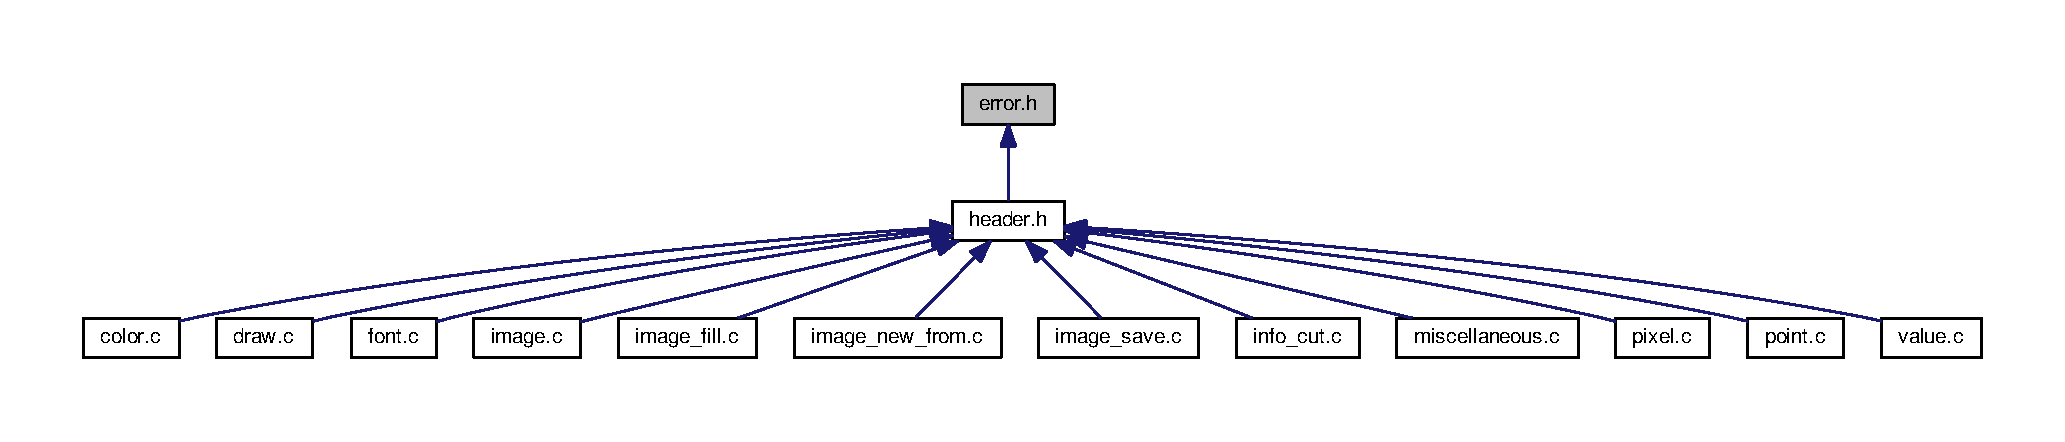
\includegraphics[width=350pt]{error_8h__dep__incl}
\end{center}
\end{figure}
\subsection*{Macros}
\begin{DoxyCompactItemize}
\item 
\#define \hyperlink{error_8h_ae413794c9d523f741b84cdd76566465b}{I\+M\+E\+L\+\_\+\+E\+R\+R\+\_\+\+L\+O\+AD}~0xa0
\item 
\#define \hyperlink{error_8h_a54c54c107af11bd0e3959bee6b494eff}{I\+M\+E\+L\+\_\+\+E\+R\+R\+\_\+\+J\+P\+E\+G\+\_\+\+L\+O\+AD}~0x60
\item 
\#define \hyperlink{error_8h_ad13d978b83348f90422fb76bd4d5fd86}{I\+M\+E\+L\+\_\+\+E\+R\+R\+\_\+\+P\+N\+G\+\_\+\+L\+O\+AD}~0x61
\item 
\#define \hyperlink{error_8h_a9d08f7b77f13c82a03a1f954608d31dd}{I\+M\+E\+L\+\_\+\+E\+R\+R\+\_\+\+T\+I\+F\+F\+\_\+\+L\+O\+AD}~0x62
\item 
\#define \hyperlink{error_8h_a655d3dce336febd1fe88fd9051950f54}{I\+M\+E\+L\+\_\+\+E\+R\+R\+\_\+\+B\+M\+P\+\_\+\+L\+O\+AD}~0x63
\item 
\#define \hyperlink{error_8h_aaf7f680ecf9737d2737214155e5f5e54}{I\+M\+E\+L\+\_\+\+E\+R\+R\+\_\+\+D\+D\+S\+\_\+\+L\+O\+AD}~0x64
\item 
\#define \hyperlink{error_8h_ae6e5a474d4bc9e050b588595f7928a10}{I\+M\+E\+L\+\_\+\+E\+R\+R\+\_\+\+F\+A\+X\+G3\+\_\+\+L\+O\+AD}~0x65
\item 
\#define \hyperlink{error_8h_a87c77fd972ffdbf48d0da6fd9046e206}{I\+M\+E\+L\+\_\+\+E\+R\+R\+\_\+\+C\+U\+T\+\_\+\+L\+O\+AD}~0x66
\item 
\#define \hyperlink{error_8h_abc341abf04ae40fd5a098308839a12eb}{I\+M\+E\+L\+\_\+\+E\+R\+R\+\_\+\+X\+P\+M\+\_\+\+L\+O\+AD}~0x67
\item 
\#define \hyperlink{error_8h_acba848b697f3cb353b8f291c06808941}{I\+M\+E\+L\+\_\+\+E\+R\+R\+\_\+\+X\+B\+M\+\_\+\+L\+O\+AD}~0x68
\item 
\#define \hyperlink{error_8h_a5b9934610ee90065d35371bf039b3774}{I\+M\+E\+L\+\_\+\+E\+R\+R\+\_\+\+S\+G\+I\+\_\+\+L\+O\+AD}~0x69
\item 
\#define \hyperlink{error_8h_ad014abe78bd5a521b1d0b2557809d871}{I\+M\+E\+L\+\_\+\+E\+R\+R\+\_\+\+W\+B\+M\+P\+\_\+\+L\+O\+AD}~0x70
\item 
\#define \hyperlink{error_8h_a00bd52766bfbc3b535ca477c700702f3}{I\+M\+E\+L\+\_\+\+E\+R\+R\+\_\+\+H\+D\+R\+\_\+\+L\+O\+AD}~0x71
\item 
\#define \hyperlink{error_8h_ad95ef8ef770f945bd11e5de1bf69d021}{I\+M\+E\+L\+\_\+\+E\+R\+R\+\_\+\+P\+S\+D\+\_\+\+L\+O\+AD}~0x72
\item 
\#define \hyperlink{error_8h_ad03bd39ddd4b3a8550e21d27c9c44734}{I\+M\+E\+L\+\_\+\+E\+R\+R\+\_\+\+I\+F\+F\+\_\+\+L\+O\+AD}~0x73
\item 
\#define \hyperlink{error_8h_aa2f98f52ce81021edf7185caa6ed65fb}{I\+M\+E\+L\+\_\+\+E\+R\+R\+\_\+\+J\+N\+G\+\_\+\+L\+O\+AD}~0x74
\item 
\#define \hyperlink{error_8h_aa750e13863b5a6f99688cddc708ef4c2}{I\+M\+E\+L\+\_\+\+E\+R\+R\+\_\+\+K\+O\+A\+L\+A\+\_\+\+L\+O\+AD}~0x75
\item 
\#define \hyperlink{error_8h_a4e035c6623d16b9f20b4bd27cad7110b}{I\+M\+E\+L\+\_\+\+E\+R\+R\+\_\+\+M\+N\+G\+\_\+\+L\+O\+AD}~0x76
\item 
\#define \hyperlink{error_8h_a7e0a5b33dd3fdfe23b715ad1f2e3d521}{I\+M\+E\+L\+\_\+\+E\+R\+R\+\_\+\+P\+C\+X\+\_\+\+L\+O\+AD}~0x77
\item 
\#define \hyperlink{error_8h_af565fd8d797c867c6c869a932ae1c36c}{I\+M\+E\+L\+\_\+\+E\+R\+R\+\_\+\+P\+G\+M\+\_\+\+L\+O\+AD}~0x78
\item 
\#define \hyperlink{error_8h_a798fa4d904df345b0e9b33fa054fe9a0}{I\+M\+E\+L\+\_\+\+E\+R\+R\+\_\+\+P\+G\+M\+R\+A\+W\+\_\+\+L\+O\+AD}~0x79
\item 
\#define \hyperlink{error_8h_adb387c06690bddb415e7fb96aad8f786}{I\+M\+E\+L\+\_\+\+E\+R\+R\+\_\+\+R\+A\+S\+\_\+\+L\+O\+AD}~0x80
\item 
\#define \hyperlink{error_8h_af0d098d8ed586429651f7f25050ae08c}{I\+M\+E\+L\+\_\+\+E\+R\+R\+\_\+\+E\+X\+R\+\_\+\+L\+O\+AD}~0x81
\item 
\#define \hyperlink{error_8h_a9615a26d77464fe68d3e56f35ed5f6c9}{I\+M\+E\+L\+\_\+\+E\+R\+R\+\_\+\+J2\+K\+\_\+\+L\+O\+AD}~0x82
\item 
\#define \hyperlink{error_8h_a987a2563d0312699154bdbad4f555ad4}{I\+M\+E\+L\+\_\+\+E\+R\+R\+\_\+\+P\+P\+M\+\_\+\+L\+O\+AD}~0x83
\item 
\#define \hyperlink{error_8h_a1512bfd1be774df8cc747a93b3091a3d}{I\+M\+E\+L\+\_\+\+E\+R\+R\+\_\+\+P\+P\+M\+R\+A\+W\+\_\+\+L\+O\+AD}~0x84
\item 
\#define \hyperlink{error_8h_abb005cde34c72a03e8fd3535c0b866b6}{I\+M\+E\+L\+\_\+\+E\+R\+R\+\_\+\+P\+B\+M\+\_\+\+L\+O\+AD}~0x85
\item 
\#define \hyperlink{error_8h_a618362cfd6320d4f1f79833208ad9fd6}{I\+M\+E\+L\+\_\+\+E\+R\+R\+\_\+\+P\+B\+M\+R\+A\+W\+\_\+\+L\+O\+AD}~0x86
\item 
\#define \hyperlink{error_8h_a2e241032c7d2590b0cd4d72490669ab5}{I\+M\+E\+L\+\_\+\+E\+R\+R\+\_\+\+T\+A\+R\+G\+A\+\_\+\+L\+O\+AD}~0x87
\item 
\#define \hyperlink{error_8h_a48885156dc8a7d4d8b138c7ccfc61c08}{I\+M\+E\+L\+\_\+\+E\+R\+R\+\_\+\+J\+P2\+\_\+\+L\+O\+AD}~0x88
\item 
\#define \hyperlink{error_8h_ad6071a1aea5ba877efa5d8a4d06352bf}{I\+M\+E\+L\+\_\+\+E\+R\+R\+\_\+\+I\+C\+O\+\_\+\+L\+O\+AD}~0x89
\item 
\#define \hyperlink{error_8h_a1e7f1727c3feb78ef7f4360940a26bae}{I\+M\+E\+L\+\_\+\+E\+R\+R\+\_\+\+P\+C\+D\+\_\+\+L\+O\+AD}~0x90
\item 
\#define \hyperlink{error_8h_ac9b1b805f88d39542c5247ceef0f360b}{I\+M\+E\+L\+\_\+\+E\+R\+R\+\_\+\+G\+I\+F\+\_\+\+L\+O\+AD}~0x91
\item 
\#define \hyperlink{error_8h_a2fa6eadb1fbef3f75c8829caf7678324}{I\+M\+E\+L\+\_\+\+E\+R\+R\+\_\+\+P\+N\+G\+\_\+\+W\+R\+I\+T\+E\+\_\+\+S\+T\+R\+U\+CT}~0x10
\item 
\#define \hyperlink{error_8h_a03e9818d6ff8a066d774c8246135e95d}{I\+M\+E\+L\+\_\+\+E\+R\+R\+\_\+\+P\+N\+G\+\_\+\+I\+N\+F\+O\+\_\+\+S\+T\+R\+U\+CT}~0x11
\item 
\#define \hyperlink{error_8h_a47e560e2b2b45dc6af242ea602b60b43}{I\+M\+E\+L\+\_\+\+E\+R\+R\+\_\+\+P\+N\+G\+\_\+\+S\+E\+T\+\_\+\+J\+MP}~0x12
\item 
\#define \hyperlink{error_8h_ac4a8e951635df61e88a23b108535d77e}{I\+M\+E\+L\+\_\+\+E\+R\+R\+\_\+\+R\+A\+W\+\_\+\+B\+PP}~0x52
\item 
\#define \hyperlink{error_8h_a9ca38129932f16444d58b487b4563deb}{I\+M\+E\+L\+\_\+\+E\+R\+R\+\_\+\+R\+A\+W\+\_\+\+L\+E\+N\+G\+TH}~0x53
\item 
\#define \hyperlink{error_8h_a576787e35b0be64b5ccf6a515098a7ff}{I\+M\+E\+L\+\_\+\+E\+R\+R\+\_\+\+R\+A\+W\+\_\+\+F\+I\+L\+E\+\_\+\+L\+E\+N\+G\+TH}~0x54
\item 
\#define \hyperlink{error_8h_a44395afff95e6bc5c2dec2a7dad1d01d}{I\+M\+E\+L\+\_\+\+E\+R\+R\+\_\+\+R\+A\+W\+\_\+\+B\+P\+P2}~0x55
\end{DoxyCompactItemize}


\subsection{Detailed Description}
This file contains error codes used by Imel library. 

\begin{DoxyAuthor}{Author}
Davide Francesco Merico 
\end{DoxyAuthor}


\subsection{Macro Definition Documentation}
\index{error.\+h@{error.\+h}!I\+M\+E\+L\+\_\+\+E\+R\+R\+\_\+\+B\+M\+P\+\_\+\+L\+O\+AD@{I\+M\+E\+L\+\_\+\+E\+R\+R\+\_\+\+B\+M\+P\+\_\+\+L\+O\+AD}}
\index{I\+M\+E\+L\+\_\+\+E\+R\+R\+\_\+\+B\+M\+P\+\_\+\+L\+O\+AD@{I\+M\+E\+L\+\_\+\+E\+R\+R\+\_\+\+B\+M\+P\+\_\+\+L\+O\+AD}!error.\+h@{error.\+h}}
\subsubsection[{\texorpdfstring{I\+M\+E\+L\+\_\+\+E\+R\+R\+\_\+\+B\+M\+P\+\_\+\+L\+O\+AD}{IMEL_ERR_BMP_LOAD}}]{\setlength{\rightskip}{0pt plus 5cm}\#define I\+M\+E\+L\+\_\+\+E\+R\+R\+\_\+\+B\+M\+P\+\_\+\+L\+O\+AD~0x63}\hypertarget{error_8h_a655d3dce336febd1fe88fd9051950f54}{}\label{error_8h_a655d3dce336febd1fe88fd9051950f54}
Error while loading the bmp image \index{error.\+h@{error.\+h}!I\+M\+E\+L\+\_\+\+E\+R\+R\+\_\+\+C\+U\+T\+\_\+\+L\+O\+AD@{I\+M\+E\+L\+\_\+\+E\+R\+R\+\_\+\+C\+U\+T\+\_\+\+L\+O\+AD}}
\index{I\+M\+E\+L\+\_\+\+E\+R\+R\+\_\+\+C\+U\+T\+\_\+\+L\+O\+AD@{I\+M\+E\+L\+\_\+\+E\+R\+R\+\_\+\+C\+U\+T\+\_\+\+L\+O\+AD}!error.\+h@{error.\+h}}
\subsubsection[{\texorpdfstring{I\+M\+E\+L\+\_\+\+E\+R\+R\+\_\+\+C\+U\+T\+\_\+\+L\+O\+AD}{IMEL_ERR_CUT_LOAD}}]{\setlength{\rightskip}{0pt plus 5cm}\#define I\+M\+E\+L\+\_\+\+E\+R\+R\+\_\+\+C\+U\+T\+\_\+\+L\+O\+AD~0x66}\hypertarget{error_8h_a87c77fd972ffdbf48d0da6fd9046e206}{}\label{error_8h_a87c77fd972ffdbf48d0da6fd9046e206}
Error while loading the cut image \index{error.\+h@{error.\+h}!I\+M\+E\+L\+\_\+\+E\+R\+R\+\_\+\+D\+D\+S\+\_\+\+L\+O\+AD@{I\+M\+E\+L\+\_\+\+E\+R\+R\+\_\+\+D\+D\+S\+\_\+\+L\+O\+AD}}
\index{I\+M\+E\+L\+\_\+\+E\+R\+R\+\_\+\+D\+D\+S\+\_\+\+L\+O\+AD@{I\+M\+E\+L\+\_\+\+E\+R\+R\+\_\+\+D\+D\+S\+\_\+\+L\+O\+AD}!error.\+h@{error.\+h}}
\subsubsection[{\texorpdfstring{I\+M\+E\+L\+\_\+\+E\+R\+R\+\_\+\+D\+D\+S\+\_\+\+L\+O\+AD}{IMEL_ERR_DDS_LOAD}}]{\setlength{\rightskip}{0pt plus 5cm}\#define I\+M\+E\+L\+\_\+\+E\+R\+R\+\_\+\+D\+D\+S\+\_\+\+L\+O\+AD~0x64}\hypertarget{error_8h_aaf7f680ecf9737d2737214155e5f5e54}{}\label{error_8h_aaf7f680ecf9737d2737214155e5f5e54}
Error while loading the dds image \index{error.\+h@{error.\+h}!I\+M\+E\+L\+\_\+\+E\+R\+R\+\_\+\+E\+X\+R\+\_\+\+L\+O\+AD@{I\+M\+E\+L\+\_\+\+E\+R\+R\+\_\+\+E\+X\+R\+\_\+\+L\+O\+AD}}
\index{I\+M\+E\+L\+\_\+\+E\+R\+R\+\_\+\+E\+X\+R\+\_\+\+L\+O\+AD@{I\+M\+E\+L\+\_\+\+E\+R\+R\+\_\+\+E\+X\+R\+\_\+\+L\+O\+AD}!error.\+h@{error.\+h}}
\subsubsection[{\texorpdfstring{I\+M\+E\+L\+\_\+\+E\+R\+R\+\_\+\+E\+X\+R\+\_\+\+L\+O\+AD}{IMEL_ERR_EXR_LOAD}}]{\setlength{\rightskip}{0pt plus 5cm}\#define I\+M\+E\+L\+\_\+\+E\+R\+R\+\_\+\+E\+X\+R\+\_\+\+L\+O\+AD~0x81}\hypertarget{error_8h_af0d098d8ed586429651f7f25050ae08c}{}\label{error_8h_af0d098d8ed586429651f7f25050ae08c}
Error while loading the exr image \index{error.\+h@{error.\+h}!I\+M\+E\+L\+\_\+\+E\+R\+R\+\_\+\+F\+A\+X\+G3\+\_\+\+L\+O\+AD@{I\+M\+E\+L\+\_\+\+E\+R\+R\+\_\+\+F\+A\+X\+G3\+\_\+\+L\+O\+AD}}
\index{I\+M\+E\+L\+\_\+\+E\+R\+R\+\_\+\+F\+A\+X\+G3\+\_\+\+L\+O\+AD@{I\+M\+E\+L\+\_\+\+E\+R\+R\+\_\+\+F\+A\+X\+G3\+\_\+\+L\+O\+AD}!error.\+h@{error.\+h}}
\subsubsection[{\texorpdfstring{I\+M\+E\+L\+\_\+\+E\+R\+R\+\_\+\+F\+A\+X\+G3\+\_\+\+L\+O\+AD}{IMEL_ERR_FAXG3_LOAD}}]{\setlength{\rightskip}{0pt plus 5cm}\#define I\+M\+E\+L\+\_\+\+E\+R\+R\+\_\+\+F\+A\+X\+G3\+\_\+\+L\+O\+AD~0x65}\hypertarget{error_8h_ae6e5a474d4bc9e050b588595f7928a10}{}\label{error_8h_ae6e5a474d4bc9e050b588595f7928a10}
Error while loading the faxg3 image \index{error.\+h@{error.\+h}!I\+M\+E\+L\+\_\+\+E\+R\+R\+\_\+\+G\+I\+F\+\_\+\+L\+O\+AD@{I\+M\+E\+L\+\_\+\+E\+R\+R\+\_\+\+G\+I\+F\+\_\+\+L\+O\+AD}}
\index{I\+M\+E\+L\+\_\+\+E\+R\+R\+\_\+\+G\+I\+F\+\_\+\+L\+O\+AD@{I\+M\+E\+L\+\_\+\+E\+R\+R\+\_\+\+G\+I\+F\+\_\+\+L\+O\+AD}!error.\+h@{error.\+h}}
\subsubsection[{\texorpdfstring{I\+M\+E\+L\+\_\+\+E\+R\+R\+\_\+\+G\+I\+F\+\_\+\+L\+O\+AD}{IMEL_ERR_GIF_LOAD}}]{\setlength{\rightskip}{0pt plus 5cm}\#define I\+M\+E\+L\+\_\+\+E\+R\+R\+\_\+\+G\+I\+F\+\_\+\+L\+O\+AD~0x91}\hypertarget{error_8h_ac9b1b805f88d39542c5247ceef0f360b}{}\label{error_8h_ac9b1b805f88d39542c5247ceef0f360b}
Error while loading the gif image \index{error.\+h@{error.\+h}!I\+M\+E\+L\+\_\+\+E\+R\+R\+\_\+\+H\+D\+R\+\_\+\+L\+O\+AD@{I\+M\+E\+L\+\_\+\+E\+R\+R\+\_\+\+H\+D\+R\+\_\+\+L\+O\+AD}}
\index{I\+M\+E\+L\+\_\+\+E\+R\+R\+\_\+\+H\+D\+R\+\_\+\+L\+O\+AD@{I\+M\+E\+L\+\_\+\+E\+R\+R\+\_\+\+H\+D\+R\+\_\+\+L\+O\+AD}!error.\+h@{error.\+h}}
\subsubsection[{\texorpdfstring{I\+M\+E\+L\+\_\+\+E\+R\+R\+\_\+\+H\+D\+R\+\_\+\+L\+O\+AD}{IMEL_ERR_HDR_LOAD}}]{\setlength{\rightskip}{0pt plus 5cm}\#define I\+M\+E\+L\+\_\+\+E\+R\+R\+\_\+\+H\+D\+R\+\_\+\+L\+O\+AD~0x71}\hypertarget{error_8h_a00bd52766bfbc3b535ca477c700702f3}{}\label{error_8h_a00bd52766bfbc3b535ca477c700702f3}
Error while loading the hdr image \index{error.\+h@{error.\+h}!I\+M\+E\+L\+\_\+\+E\+R\+R\+\_\+\+I\+C\+O\+\_\+\+L\+O\+AD@{I\+M\+E\+L\+\_\+\+E\+R\+R\+\_\+\+I\+C\+O\+\_\+\+L\+O\+AD}}
\index{I\+M\+E\+L\+\_\+\+E\+R\+R\+\_\+\+I\+C\+O\+\_\+\+L\+O\+AD@{I\+M\+E\+L\+\_\+\+E\+R\+R\+\_\+\+I\+C\+O\+\_\+\+L\+O\+AD}!error.\+h@{error.\+h}}
\subsubsection[{\texorpdfstring{I\+M\+E\+L\+\_\+\+E\+R\+R\+\_\+\+I\+C\+O\+\_\+\+L\+O\+AD}{IMEL_ERR_ICO_LOAD}}]{\setlength{\rightskip}{0pt plus 5cm}\#define I\+M\+E\+L\+\_\+\+E\+R\+R\+\_\+\+I\+C\+O\+\_\+\+L\+O\+AD~0x89}\hypertarget{error_8h_ad6071a1aea5ba877efa5d8a4d06352bf}{}\label{error_8h_ad6071a1aea5ba877efa5d8a4d06352bf}
Error while loading the ico image \index{error.\+h@{error.\+h}!I\+M\+E\+L\+\_\+\+E\+R\+R\+\_\+\+I\+F\+F\+\_\+\+L\+O\+AD@{I\+M\+E\+L\+\_\+\+E\+R\+R\+\_\+\+I\+F\+F\+\_\+\+L\+O\+AD}}
\index{I\+M\+E\+L\+\_\+\+E\+R\+R\+\_\+\+I\+F\+F\+\_\+\+L\+O\+AD@{I\+M\+E\+L\+\_\+\+E\+R\+R\+\_\+\+I\+F\+F\+\_\+\+L\+O\+AD}!error.\+h@{error.\+h}}
\subsubsection[{\texorpdfstring{I\+M\+E\+L\+\_\+\+E\+R\+R\+\_\+\+I\+F\+F\+\_\+\+L\+O\+AD}{IMEL_ERR_IFF_LOAD}}]{\setlength{\rightskip}{0pt plus 5cm}\#define I\+M\+E\+L\+\_\+\+E\+R\+R\+\_\+\+I\+F\+F\+\_\+\+L\+O\+AD~0x73}\hypertarget{error_8h_ad03bd39ddd4b3a8550e21d27c9c44734}{}\label{error_8h_ad03bd39ddd4b3a8550e21d27c9c44734}
Error while loading the iff image \index{error.\+h@{error.\+h}!I\+M\+E\+L\+\_\+\+E\+R\+R\+\_\+\+J2\+K\+\_\+\+L\+O\+AD@{I\+M\+E\+L\+\_\+\+E\+R\+R\+\_\+\+J2\+K\+\_\+\+L\+O\+AD}}
\index{I\+M\+E\+L\+\_\+\+E\+R\+R\+\_\+\+J2\+K\+\_\+\+L\+O\+AD@{I\+M\+E\+L\+\_\+\+E\+R\+R\+\_\+\+J2\+K\+\_\+\+L\+O\+AD}!error.\+h@{error.\+h}}
\subsubsection[{\texorpdfstring{I\+M\+E\+L\+\_\+\+E\+R\+R\+\_\+\+J2\+K\+\_\+\+L\+O\+AD}{IMEL_ERR_J2K_LOAD}}]{\setlength{\rightskip}{0pt plus 5cm}\#define I\+M\+E\+L\+\_\+\+E\+R\+R\+\_\+\+J2\+K\+\_\+\+L\+O\+AD~0x82}\hypertarget{error_8h_a9615a26d77464fe68d3e56f35ed5f6c9}{}\label{error_8h_a9615a26d77464fe68d3e56f35ed5f6c9}
Error while loading the j2k image \index{error.\+h@{error.\+h}!I\+M\+E\+L\+\_\+\+E\+R\+R\+\_\+\+J\+N\+G\+\_\+\+L\+O\+AD@{I\+M\+E\+L\+\_\+\+E\+R\+R\+\_\+\+J\+N\+G\+\_\+\+L\+O\+AD}}
\index{I\+M\+E\+L\+\_\+\+E\+R\+R\+\_\+\+J\+N\+G\+\_\+\+L\+O\+AD@{I\+M\+E\+L\+\_\+\+E\+R\+R\+\_\+\+J\+N\+G\+\_\+\+L\+O\+AD}!error.\+h@{error.\+h}}
\subsubsection[{\texorpdfstring{I\+M\+E\+L\+\_\+\+E\+R\+R\+\_\+\+J\+N\+G\+\_\+\+L\+O\+AD}{IMEL_ERR_JNG_LOAD}}]{\setlength{\rightskip}{0pt plus 5cm}\#define I\+M\+E\+L\+\_\+\+E\+R\+R\+\_\+\+J\+N\+G\+\_\+\+L\+O\+AD~0x74}\hypertarget{error_8h_aa2f98f52ce81021edf7185caa6ed65fb}{}\label{error_8h_aa2f98f52ce81021edf7185caa6ed65fb}
Error while loading the jng image \index{error.\+h@{error.\+h}!I\+M\+E\+L\+\_\+\+E\+R\+R\+\_\+\+J\+P2\+\_\+\+L\+O\+AD@{I\+M\+E\+L\+\_\+\+E\+R\+R\+\_\+\+J\+P2\+\_\+\+L\+O\+AD}}
\index{I\+M\+E\+L\+\_\+\+E\+R\+R\+\_\+\+J\+P2\+\_\+\+L\+O\+AD@{I\+M\+E\+L\+\_\+\+E\+R\+R\+\_\+\+J\+P2\+\_\+\+L\+O\+AD}!error.\+h@{error.\+h}}
\subsubsection[{\texorpdfstring{I\+M\+E\+L\+\_\+\+E\+R\+R\+\_\+\+J\+P2\+\_\+\+L\+O\+AD}{IMEL_ERR_JP2_LOAD}}]{\setlength{\rightskip}{0pt plus 5cm}\#define I\+M\+E\+L\+\_\+\+E\+R\+R\+\_\+\+J\+P2\+\_\+\+L\+O\+AD~0x88}\hypertarget{error_8h_a48885156dc8a7d4d8b138c7ccfc61c08}{}\label{error_8h_a48885156dc8a7d4d8b138c7ccfc61c08}
Error while loading the jp2 image \index{error.\+h@{error.\+h}!I\+M\+E\+L\+\_\+\+E\+R\+R\+\_\+\+J\+P\+E\+G\+\_\+\+L\+O\+AD@{I\+M\+E\+L\+\_\+\+E\+R\+R\+\_\+\+J\+P\+E\+G\+\_\+\+L\+O\+AD}}
\index{I\+M\+E\+L\+\_\+\+E\+R\+R\+\_\+\+J\+P\+E\+G\+\_\+\+L\+O\+AD@{I\+M\+E\+L\+\_\+\+E\+R\+R\+\_\+\+J\+P\+E\+G\+\_\+\+L\+O\+AD}!error.\+h@{error.\+h}}
\subsubsection[{\texorpdfstring{I\+M\+E\+L\+\_\+\+E\+R\+R\+\_\+\+J\+P\+E\+G\+\_\+\+L\+O\+AD}{IMEL_ERR_JPEG_LOAD}}]{\setlength{\rightskip}{0pt plus 5cm}\#define I\+M\+E\+L\+\_\+\+E\+R\+R\+\_\+\+J\+P\+E\+G\+\_\+\+L\+O\+AD~0x60}\hypertarget{error_8h_a54c54c107af11bd0e3959bee6b494eff}{}\label{error_8h_a54c54c107af11bd0e3959bee6b494eff}
Error while loading the jpeg image \index{error.\+h@{error.\+h}!I\+M\+E\+L\+\_\+\+E\+R\+R\+\_\+\+K\+O\+A\+L\+A\+\_\+\+L\+O\+AD@{I\+M\+E\+L\+\_\+\+E\+R\+R\+\_\+\+K\+O\+A\+L\+A\+\_\+\+L\+O\+AD}}
\index{I\+M\+E\+L\+\_\+\+E\+R\+R\+\_\+\+K\+O\+A\+L\+A\+\_\+\+L\+O\+AD@{I\+M\+E\+L\+\_\+\+E\+R\+R\+\_\+\+K\+O\+A\+L\+A\+\_\+\+L\+O\+AD}!error.\+h@{error.\+h}}
\subsubsection[{\texorpdfstring{I\+M\+E\+L\+\_\+\+E\+R\+R\+\_\+\+K\+O\+A\+L\+A\+\_\+\+L\+O\+AD}{IMEL_ERR_KOALA_LOAD}}]{\setlength{\rightskip}{0pt plus 5cm}\#define I\+M\+E\+L\+\_\+\+E\+R\+R\+\_\+\+K\+O\+A\+L\+A\+\_\+\+L\+O\+AD~0x75}\hypertarget{error_8h_aa750e13863b5a6f99688cddc708ef4c2}{}\label{error_8h_aa750e13863b5a6f99688cddc708ef4c2}
Error while loading the koala image \index{error.\+h@{error.\+h}!I\+M\+E\+L\+\_\+\+E\+R\+R\+\_\+\+L\+O\+AD@{I\+M\+E\+L\+\_\+\+E\+R\+R\+\_\+\+L\+O\+AD}}
\index{I\+M\+E\+L\+\_\+\+E\+R\+R\+\_\+\+L\+O\+AD@{I\+M\+E\+L\+\_\+\+E\+R\+R\+\_\+\+L\+O\+AD}!error.\+h@{error.\+h}}
\subsubsection[{\texorpdfstring{I\+M\+E\+L\+\_\+\+E\+R\+R\+\_\+\+L\+O\+AD}{IMEL_ERR_LOAD}}]{\setlength{\rightskip}{0pt plus 5cm}\#define I\+M\+E\+L\+\_\+\+E\+R\+R\+\_\+\+L\+O\+AD~0xa0}\hypertarget{error_8h_ae413794c9d523f741b84cdd76566465b}{}\label{error_8h_ae413794c9d523f741b84cdd76566465b}
Error while loading the image \index{error.\+h@{error.\+h}!I\+M\+E\+L\+\_\+\+E\+R\+R\+\_\+\+M\+N\+G\+\_\+\+L\+O\+AD@{I\+M\+E\+L\+\_\+\+E\+R\+R\+\_\+\+M\+N\+G\+\_\+\+L\+O\+AD}}
\index{I\+M\+E\+L\+\_\+\+E\+R\+R\+\_\+\+M\+N\+G\+\_\+\+L\+O\+AD@{I\+M\+E\+L\+\_\+\+E\+R\+R\+\_\+\+M\+N\+G\+\_\+\+L\+O\+AD}!error.\+h@{error.\+h}}
\subsubsection[{\texorpdfstring{I\+M\+E\+L\+\_\+\+E\+R\+R\+\_\+\+M\+N\+G\+\_\+\+L\+O\+AD}{IMEL_ERR_MNG_LOAD}}]{\setlength{\rightskip}{0pt plus 5cm}\#define I\+M\+E\+L\+\_\+\+E\+R\+R\+\_\+\+M\+N\+G\+\_\+\+L\+O\+AD~0x76}\hypertarget{error_8h_a4e035c6623d16b9f20b4bd27cad7110b}{}\label{error_8h_a4e035c6623d16b9f20b4bd27cad7110b}
Error while loading the mng image \index{error.\+h@{error.\+h}!I\+M\+E\+L\+\_\+\+E\+R\+R\+\_\+\+P\+B\+M\+\_\+\+L\+O\+AD@{I\+M\+E\+L\+\_\+\+E\+R\+R\+\_\+\+P\+B\+M\+\_\+\+L\+O\+AD}}
\index{I\+M\+E\+L\+\_\+\+E\+R\+R\+\_\+\+P\+B\+M\+\_\+\+L\+O\+AD@{I\+M\+E\+L\+\_\+\+E\+R\+R\+\_\+\+P\+B\+M\+\_\+\+L\+O\+AD}!error.\+h@{error.\+h}}
\subsubsection[{\texorpdfstring{I\+M\+E\+L\+\_\+\+E\+R\+R\+\_\+\+P\+B\+M\+\_\+\+L\+O\+AD}{IMEL_ERR_PBM_LOAD}}]{\setlength{\rightskip}{0pt plus 5cm}\#define I\+M\+E\+L\+\_\+\+E\+R\+R\+\_\+\+P\+B\+M\+\_\+\+L\+O\+AD~0x85}\hypertarget{error_8h_abb005cde34c72a03e8fd3535c0b866b6}{}\label{error_8h_abb005cde34c72a03e8fd3535c0b866b6}
Error while loading the pbm image \index{error.\+h@{error.\+h}!I\+M\+E\+L\+\_\+\+E\+R\+R\+\_\+\+P\+B\+M\+R\+A\+W\+\_\+\+L\+O\+AD@{I\+M\+E\+L\+\_\+\+E\+R\+R\+\_\+\+P\+B\+M\+R\+A\+W\+\_\+\+L\+O\+AD}}
\index{I\+M\+E\+L\+\_\+\+E\+R\+R\+\_\+\+P\+B\+M\+R\+A\+W\+\_\+\+L\+O\+AD@{I\+M\+E\+L\+\_\+\+E\+R\+R\+\_\+\+P\+B\+M\+R\+A\+W\+\_\+\+L\+O\+AD}!error.\+h@{error.\+h}}
\subsubsection[{\texorpdfstring{I\+M\+E\+L\+\_\+\+E\+R\+R\+\_\+\+P\+B\+M\+R\+A\+W\+\_\+\+L\+O\+AD}{IMEL_ERR_PBMRAW_LOAD}}]{\setlength{\rightskip}{0pt plus 5cm}\#define I\+M\+E\+L\+\_\+\+E\+R\+R\+\_\+\+P\+B\+M\+R\+A\+W\+\_\+\+L\+O\+AD~0x86}\hypertarget{error_8h_a618362cfd6320d4f1f79833208ad9fd6}{}\label{error_8h_a618362cfd6320d4f1f79833208ad9fd6}
Error while loading the pbmraw image \index{error.\+h@{error.\+h}!I\+M\+E\+L\+\_\+\+E\+R\+R\+\_\+\+P\+C\+D\+\_\+\+L\+O\+AD@{I\+M\+E\+L\+\_\+\+E\+R\+R\+\_\+\+P\+C\+D\+\_\+\+L\+O\+AD}}
\index{I\+M\+E\+L\+\_\+\+E\+R\+R\+\_\+\+P\+C\+D\+\_\+\+L\+O\+AD@{I\+M\+E\+L\+\_\+\+E\+R\+R\+\_\+\+P\+C\+D\+\_\+\+L\+O\+AD}!error.\+h@{error.\+h}}
\subsubsection[{\texorpdfstring{I\+M\+E\+L\+\_\+\+E\+R\+R\+\_\+\+P\+C\+D\+\_\+\+L\+O\+AD}{IMEL_ERR_PCD_LOAD}}]{\setlength{\rightskip}{0pt plus 5cm}\#define I\+M\+E\+L\+\_\+\+E\+R\+R\+\_\+\+P\+C\+D\+\_\+\+L\+O\+AD~0x90}\hypertarget{error_8h_a1e7f1727c3feb78ef7f4360940a26bae}{}\label{error_8h_a1e7f1727c3feb78ef7f4360940a26bae}
Error while loading the pcd image \index{error.\+h@{error.\+h}!I\+M\+E\+L\+\_\+\+E\+R\+R\+\_\+\+P\+C\+X\+\_\+\+L\+O\+AD@{I\+M\+E\+L\+\_\+\+E\+R\+R\+\_\+\+P\+C\+X\+\_\+\+L\+O\+AD}}
\index{I\+M\+E\+L\+\_\+\+E\+R\+R\+\_\+\+P\+C\+X\+\_\+\+L\+O\+AD@{I\+M\+E\+L\+\_\+\+E\+R\+R\+\_\+\+P\+C\+X\+\_\+\+L\+O\+AD}!error.\+h@{error.\+h}}
\subsubsection[{\texorpdfstring{I\+M\+E\+L\+\_\+\+E\+R\+R\+\_\+\+P\+C\+X\+\_\+\+L\+O\+AD}{IMEL_ERR_PCX_LOAD}}]{\setlength{\rightskip}{0pt plus 5cm}\#define I\+M\+E\+L\+\_\+\+E\+R\+R\+\_\+\+P\+C\+X\+\_\+\+L\+O\+AD~0x77}\hypertarget{error_8h_a7e0a5b33dd3fdfe23b715ad1f2e3d521}{}\label{error_8h_a7e0a5b33dd3fdfe23b715ad1f2e3d521}
Error while loading the pcx image \index{error.\+h@{error.\+h}!I\+M\+E\+L\+\_\+\+E\+R\+R\+\_\+\+P\+G\+M\+\_\+\+L\+O\+AD@{I\+M\+E\+L\+\_\+\+E\+R\+R\+\_\+\+P\+G\+M\+\_\+\+L\+O\+AD}}
\index{I\+M\+E\+L\+\_\+\+E\+R\+R\+\_\+\+P\+G\+M\+\_\+\+L\+O\+AD@{I\+M\+E\+L\+\_\+\+E\+R\+R\+\_\+\+P\+G\+M\+\_\+\+L\+O\+AD}!error.\+h@{error.\+h}}
\subsubsection[{\texorpdfstring{I\+M\+E\+L\+\_\+\+E\+R\+R\+\_\+\+P\+G\+M\+\_\+\+L\+O\+AD}{IMEL_ERR_PGM_LOAD}}]{\setlength{\rightskip}{0pt plus 5cm}\#define I\+M\+E\+L\+\_\+\+E\+R\+R\+\_\+\+P\+G\+M\+\_\+\+L\+O\+AD~0x78}\hypertarget{error_8h_af565fd8d797c867c6c869a932ae1c36c}{}\label{error_8h_af565fd8d797c867c6c869a932ae1c36c}
Error while loading the pgm image \index{error.\+h@{error.\+h}!I\+M\+E\+L\+\_\+\+E\+R\+R\+\_\+\+P\+G\+M\+R\+A\+W\+\_\+\+L\+O\+AD@{I\+M\+E\+L\+\_\+\+E\+R\+R\+\_\+\+P\+G\+M\+R\+A\+W\+\_\+\+L\+O\+AD}}
\index{I\+M\+E\+L\+\_\+\+E\+R\+R\+\_\+\+P\+G\+M\+R\+A\+W\+\_\+\+L\+O\+AD@{I\+M\+E\+L\+\_\+\+E\+R\+R\+\_\+\+P\+G\+M\+R\+A\+W\+\_\+\+L\+O\+AD}!error.\+h@{error.\+h}}
\subsubsection[{\texorpdfstring{I\+M\+E\+L\+\_\+\+E\+R\+R\+\_\+\+P\+G\+M\+R\+A\+W\+\_\+\+L\+O\+AD}{IMEL_ERR_PGMRAW_LOAD}}]{\setlength{\rightskip}{0pt plus 5cm}\#define I\+M\+E\+L\+\_\+\+E\+R\+R\+\_\+\+P\+G\+M\+R\+A\+W\+\_\+\+L\+O\+AD~0x79}\hypertarget{error_8h_a798fa4d904df345b0e9b33fa054fe9a0}{}\label{error_8h_a798fa4d904df345b0e9b33fa054fe9a0}
Error while loading the pgmraw image \index{error.\+h@{error.\+h}!I\+M\+E\+L\+\_\+\+E\+R\+R\+\_\+\+P\+N\+G\+\_\+\+I\+N\+F\+O\+\_\+\+S\+T\+R\+U\+CT@{I\+M\+E\+L\+\_\+\+E\+R\+R\+\_\+\+P\+N\+G\+\_\+\+I\+N\+F\+O\+\_\+\+S\+T\+R\+U\+CT}}
\index{I\+M\+E\+L\+\_\+\+E\+R\+R\+\_\+\+P\+N\+G\+\_\+\+I\+N\+F\+O\+\_\+\+S\+T\+R\+U\+CT@{I\+M\+E\+L\+\_\+\+E\+R\+R\+\_\+\+P\+N\+G\+\_\+\+I\+N\+F\+O\+\_\+\+S\+T\+R\+U\+CT}!error.\+h@{error.\+h}}
\subsubsection[{\texorpdfstring{I\+M\+E\+L\+\_\+\+E\+R\+R\+\_\+\+P\+N\+G\+\_\+\+I\+N\+F\+O\+\_\+\+S\+T\+R\+U\+CT}{IMEL_ERR_PNG_INFO_STRUCT}}]{\setlength{\rightskip}{0pt plus 5cm}\#define I\+M\+E\+L\+\_\+\+E\+R\+R\+\_\+\+P\+N\+G\+\_\+\+I\+N\+F\+O\+\_\+\+S\+T\+R\+U\+CT~0x11}\hypertarget{error_8h_a03e9818d6ff8a066d774c8246135e95d}{}\label{error_8h_a03e9818d6ff8a066d774c8246135e95d}
Could not create P\+NG info structure (out of memory?) \index{error.\+h@{error.\+h}!I\+M\+E\+L\+\_\+\+E\+R\+R\+\_\+\+P\+N\+G\+\_\+\+L\+O\+AD@{I\+M\+E\+L\+\_\+\+E\+R\+R\+\_\+\+P\+N\+G\+\_\+\+L\+O\+AD}}
\index{I\+M\+E\+L\+\_\+\+E\+R\+R\+\_\+\+P\+N\+G\+\_\+\+L\+O\+AD@{I\+M\+E\+L\+\_\+\+E\+R\+R\+\_\+\+P\+N\+G\+\_\+\+L\+O\+AD}!error.\+h@{error.\+h}}
\subsubsection[{\texorpdfstring{I\+M\+E\+L\+\_\+\+E\+R\+R\+\_\+\+P\+N\+G\+\_\+\+L\+O\+AD}{IMEL_ERR_PNG_LOAD}}]{\setlength{\rightskip}{0pt plus 5cm}\#define I\+M\+E\+L\+\_\+\+E\+R\+R\+\_\+\+P\+N\+G\+\_\+\+L\+O\+AD~0x61}\hypertarget{error_8h_ad13d978b83348f90422fb76bd4d5fd86}{}\label{error_8h_ad13d978b83348f90422fb76bd4d5fd86}
Error while loading the png image \index{error.\+h@{error.\+h}!I\+M\+E\+L\+\_\+\+E\+R\+R\+\_\+\+P\+N\+G\+\_\+\+S\+E\+T\+\_\+\+J\+MP@{I\+M\+E\+L\+\_\+\+E\+R\+R\+\_\+\+P\+N\+G\+\_\+\+S\+E\+T\+\_\+\+J\+MP}}
\index{I\+M\+E\+L\+\_\+\+E\+R\+R\+\_\+\+P\+N\+G\+\_\+\+S\+E\+T\+\_\+\+J\+MP@{I\+M\+E\+L\+\_\+\+E\+R\+R\+\_\+\+P\+N\+G\+\_\+\+S\+E\+T\+\_\+\+J\+MP}!error.\+h@{error.\+h}}
\subsubsection[{\texorpdfstring{I\+M\+E\+L\+\_\+\+E\+R\+R\+\_\+\+P\+N\+G\+\_\+\+S\+E\+T\+\_\+\+J\+MP}{IMEL_ERR_PNG_SET_JMP}}]{\setlength{\rightskip}{0pt plus 5cm}\#define I\+M\+E\+L\+\_\+\+E\+R\+R\+\_\+\+P\+N\+G\+\_\+\+S\+E\+T\+\_\+\+J\+MP~0x12}\hypertarget{error_8h_a47e560e2b2b45dc6af242ea602b60b43}{}\label{error_8h_a47e560e2b2b45dc6af242ea602b60b43}
Could not set P\+NG jump value \index{error.\+h@{error.\+h}!I\+M\+E\+L\+\_\+\+E\+R\+R\+\_\+\+P\+N\+G\+\_\+\+W\+R\+I\+T\+E\+\_\+\+S\+T\+R\+U\+CT@{I\+M\+E\+L\+\_\+\+E\+R\+R\+\_\+\+P\+N\+G\+\_\+\+W\+R\+I\+T\+E\+\_\+\+S\+T\+R\+U\+CT}}
\index{I\+M\+E\+L\+\_\+\+E\+R\+R\+\_\+\+P\+N\+G\+\_\+\+W\+R\+I\+T\+E\+\_\+\+S\+T\+R\+U\+CT@{I\+M\+E\+L\+\_\+\+E\+R\+R\+\_\+\+P\+N\+G\+\_\+\+W\+R\+I\+T\+E\+\_\+\+S\+T\+R\+U\+CT}!error.\+h@{error.\+h}}
\subsubsection[{\texorpdfstring{I\+M\+E\+L\+\_\+\+E\+R\+R\+\_\+\+P\+N\+G\+\_\+\+W\+R\+I\+T\+E\+\_\+\+S\+T\+R\+U\+CT}{IMEL_ERR_PNG_WRITE_STRUCT}}]{\setlength{\rightskip}{0pt plus 5cm}\#define I\+M\+E\+L\+\_\+\+E\+R\+R\+\_\+\+P\+N\+G\+\_\+\+W\+R\+I\+T\+E\+\_\+\+S\+T\+R\+U\+CT~0x10}\hypertarget{error_8h_a2fa6eadb1fbef3f75c8829caf7678324}{}\label{error_8h_a2fa6eadb1fbef3f75c8829caf7678324}
Could not create a P\+NG write structure (out of memory?) \index{error.\+h@{error.\+h}!I\+M\+E\+L\+\_\+\+E\+R\+R\+\_\+\+P\+P\+M\+\_\+\+L\+O\+AD@{I\+M\+E\+L\+\_\+\+E\+R\+R\+\_\+\+P\+P\+M\+\_\+\+L\+O\+AD}}
\index{I\+M\+E\+L\+\_\+\+E\+R\+R\+\_\+\+P\+P\+M\+\_\+\+L\+O\+AD@{I\+M\+E\+L\+\_\+\+E\+R\+R\+\_\+\+P\+P\+M\+\_\+\+L\+O\+AD}!error.\+h@{error.\+h}}
\subsubsection[{\texorpdfstring{I\+M\+E\+L\+\_\+\+E\+R\+R\+\_\+\+P\+P\+M\+\_\+\+L\+O\+AD}{IMEL_ERR_PPM_LOAD}}]{\setlength{\rightskip}{0pt plus 5cm}\#define I\+M\+E\+L\+\_\+\+E\+R\+R\+\_\+\+P\+P\+M\+\_\+\+L\+O\+AD~0x83}\hypertarget{error_8h_a987a2563d0312699154bdbad4f555ad4}{}\label{error_8h_a987a2563d0312699154bdbad4f555ad4}
Error while loading the ppm image \index{error.\+h@{error.\+h}!I\+M\+E\+L\+\_\+\+E\+R\+R\+\_\+\+P\+P\+M\+R\+A\+W\+\_\+\+L\+O\+AD@{I\+M\+E\+L\+\_\+\+E\+R\+R\+\_\+\+P\+P\+M\+R\+A\+W\+\_\+\+L\+O\+AD}}
\index{I\+M\+E\+L\+\_\+\+E\+R\+R\+\_\+\+P\+P\+M\+R\+A\+W\+\_\+\+L\+O\+AD@{I\+M\+E\+L\+\_\+\+E\+R\+R\+\_\+\+P\+P\+M\+R\+A\+W\+\_\+\+L\+O\+AD}!error.\+h@{error.\+h}}
\subsubsection[{\texorpdfstring{I\+M\+E\+L\+\_\+\+E\+R\+R\+\_\+\+P\+P\+M\+R\+A\+W\+\_\+\+L\+O\+AD}{IMEL_ERR_PPMRAW_LOAD}}]{\setlength{\rightskip}{0pt plus 5cm}\#define I\+M\+E\+L\+\_\+\+E\+R\+R\+\_\+\+P\+P\+M\+R\+A\+W\+\_\+\+L\+O\+AD~0x84}\hypertarget{error_8h_a1512bfd1be774df8cc747a93b3091a3d}{}\label{error_8h_a1512bfd1be774df8cc747a93b3091a3d}
Error while loading the ppmraw image \index{error.\+h@{error.\+h}!I\+M\+E\+L\+\_\+\+E\+R\+R\+\_\+\+P\+S\+D\+\_\+\+L\+O\+AD@{I\+M\+E\+L\+\_\+\+E\+R\+R\+\_\+\+P\+S\+D\+\_\+\+L\+O\+AD}}
\index{I\+M\+E\+L\+\_\+\+E\+R\+R\+\_\+\+P\+S\+D\+\_\+\+L\+O\+AD@{I\+M\+E\+L\+\_\+\+E\+R\+R\+\_\+\+P\+S\+D\+\_\+\+L\+O\+AD}!error.\+h@{error.\+h}}
\subsubsection[{\texorpdfstring{I\+M\+E\+L\+\_\+\+E\+R\+R\+\_\+\+P\+S\+D\+\_\+\+L\+O\+AD}{IMEL_ERR_PSD_LOAD}}]{\setlength{\rightskip}{0pt plus 5cm}\#define I\+M\+E\+L\+\_\+\+E\+R\+R\+\_\+\+P\+S\+D\+\_\+\+L\+O\+AD~0x72}\hypertarget{error_8h_ad95ef8ef770f945bd11e5de1bf69d021}{}\label{error_8h_ad95ef8ef770f945bd11e5de1bf69d021}
Error while loading the psd image \index{error.\+h@{error.\+h}!I\+M\+E\+L\+\_\+\+E\+R\+R\+\_\+\+R\+A\+S\+\_\+\+L\+O\+AD@{I\+M\+E\+L\+\_\+\+E\+R\+R\+\_\+\+R\+A\+S\+\_\+\+L\+O\+AD}}
\index{I\+M\+E\+L\+\_\+\+E\+R\+R\+\_\+\+R\+A\+S\+\_\+\+L\+O\+AD@{I\+M\+E\+L\+\_\+\+E\+R\+R\+\_\+\+R\+A\+S\+\_\+\+L\+O\+AD}!error.\+h@{error.\+h}}
\subsubsection[{\texorpdfstring{I\+M\+E\+L\+\_\+\+E\+R\+R\+\_\+\+R\+A\+S\+\_\+\+L\+O\+AD}{IMEL_ERR_RAS_LOAD}}]{\setlength{\rightskip}{0pt plus 5cm}\#define I\+M\+E\+L\+\_\+\+E\+R\+R\+\_\+\+R\+A\+S\+\_\+\+L\+O\+AD~0x80}\hypertarget{error_8h_adb387c06690bddb415e7fb96aad8f786}{}\label{error_8h_adb387c06690bddb415e7fb96aad8f786}
Error while loading the ras image \index{error.\+h@{error.\+h}!I\+M\+E\+L\+\_\+\+E\+R\+R\+\_\+\+R\+A\+W\+\_\+\+B\+PP@{I\+M\+E\+L\+\_\+\+E\+R\+R\+\_\+\+R\+A\+W\+\_\+\+B\+PP}}
\index{I\+M\+E\+L\+\_\+\+E\+R\+R\+\_\+\+R\+A\+W\+\_\+\+B\+PP@{I\+M\+E\+L\+\_\+\+E\+R\+R\+\_\+\+R\+A\+W\+\_\+\+B\+PP}!error.\+h@{error.\+h}}
\subsubsection[{\texorpdfstring{I\+M\+E\+L\+\_\+\+E\+R\+R\+\_\+\+R\+A\+W\+\_\+\+B\+PP}{IMEL_ERR_RAW_BPP}}]{\setlength{\rightskip}{0pt plus 5cm}\#define I\+M\+E\+L\+\_\+\+E\+R\+R\+\_\+\+R\+A\+W\+\_\+\+B\+PP~0x52}\hypertarget{error_8h_ac4a8e951635df61e88a23b108535d77e}{}\label{error_8h_ac4a8e951635df61e88a23b108535d77e}
The bpp are too big for Imel. \index{error.\+h@{error.\+h}!I\+M\+E\+L\+\_\+\+E\+R\+R\+\_\+\+R\+A\+W\+\_\+\+B\+P\+P2@{I\+M\+E\+L\+\_\+\+E\+R\+R\+\_\+\+R\+A\+W\+\_\+\+B\+P\+P2}}
\index{I\+M\+E\+L\+\_\+\+E\+R\+R\+\_\+\+R\+A\+W\+\_\+\+B\+P\+P2@{I\+M\+E\+L\+\_\+\+E\+R\+R\+\_\+\+R\+A\+W\+\_\+\+B\+P\+P2}!error.\+h@{error.\+h}}
\subsubsection[{\texorpdfstring{I\+M\+E\+L\+\_\+\+E\+R\+R\+\_\+\+R\+A\+W\+\_\+\+B\+P\+P2}{IMEL_ERR_RAW_BPP2}}]{\setlength{\rightskip}{0pt plus 5cm}\#define I\+M\+E\+L\+\_\+\+E\+R\+R\+\_\+\+R\+A\+W\+\_\+\+B\+P\+P2~0x55}\hypertarget{error_8h_a44395afff95e6bc5c2dec2a7dad1d01d}{}\label{error_8h_a44395afff95e6bc5c2dec2a7dad1d01d}
bpp equal to zero ( not valid ). \index{error.\+h@{error.\+h}!I\+M\+E\+L\+\_\+\+E\+R\+R\+\_\+\+R\+A\+W\+\_\+\+F\+I\+L\+E\+\_\+\+L\+E\+N\+G\+TH@{I\+M\+E\+L\+\_\+\+E\+R\+R\+\_\+\+R\+A\+W\+\_\+\+F\+I\+L\+E\+\_\+\+L\+E\+N\+G\+TH}}
\index{I\+M\+E\+L\+\_\+\+E\+R\+R\+\_\+\+R\+A\+W\+\_\+\+F\+I\+L\+E\+\_\+\+L\+E\+N\+G\+TH@{I\+M\+E\+L\+\_\+\+E\+R\+R\+\_\+\+R\+A\+W\+\_\+\+F\+I\+L\+E\+\_\+\+L\+E\+N\+G\+TH}!error.\+h@{error.\+h}}
\subsubsection[{\texorpdfstring{I\+M\+E\+L\+\_\+\+E\+R\+R\+\_\+\+R\+A\+W\+\_\+\+F\+I\+L\+E\+\_\+\+L\+E\+N\+G\+TH}{IMEL_ERR_RAW_FILE_LENGTH}}]{\setlength{\rightskip}{0pt plus 5cm}\#define I\+M\+E\+L\+\_\+\+E\+R\+R\+\_\+\+R\+A\+W\+\_\+\+F\+I\+L\+E\+\_\+\+L\+E\+N\+G\+TH~0x54}\hypertarget{error_8h_a576787e35b0be64b5ccf6a515098a7ff}{}\label{error_8h_a576787e35b0be64b5ccf6a515098a7ff}
The file length isn\textquotesingle{}t valid. \index{error.\+h@{error.\+h}!I\+M\+E\+L\+\_\+\+E\+R\+R\+\_\+\+R\+A\+W\+\_\+\+L\+E\+N\+G\+TH@{I\+M\+E\+L\+\_\+\+E\+R\+R\+\_\+\+R\+A\+W\+\_\+\+L\+E\+N\+G\+TH}}
\index{I\+M\+E\+L\+\_\+\+E\+R\+R\+\_\+\+R\+A\+W\+\_\+\+L\+E\+N\+G\+TH@{I\+M\+E\+L\+\_\+\+E\+R\+R\+\_\+\+R\+A\+W\+\_\+\+L\+E\+N\+G\+TH}!error.\+h@{error.\+h}}
\subsubsection[{\texorpdfstring{I\+M\+E\+L\+\_\+\+E\+R\+R\+\_\+\+R\+A\+W\+\_\+\+L\+E\+N\+G\+TH}{IMEL_ERR_RAW_LENGTH}}]{\setlength{\rightskip}{0pt plus 5cm}\#define I\+M\+E\+L\+\_\+\+E\+R\+R\+\_\+\+R\+A\+W\+\_\+\+L\+E\+N\+G\+TH~0x53}\hypertarget{error_8h_a9ca38129932f16444d58b487b4563deb}{}\label{error_8h_a9ca38129932f16444d58b487b4563deb}
The bpp aren\textquotesingle{}t multiples of 8. \index{error.\+h@{error.\+h}!I\+M\+E\+L\+\_\+\+E\+R\+R\+\_\+\+S\+G\+I\+\_\+\+L\+O\+AD@{I\+M\+E\+L\+\_\+\+E\+R\+R\+\_\+\+S\+G\+I\+\_\+\+L\+O\+AD}}
\index{I\+M\+E\+L\+\_\+\+E\+R\+R\+\_\+\+S\+G\+I\+\_\+\+L\+O\+AD@{I\+M\+E\+L\+\_\+\+E\+R\+R\+\_\+\+S\+G\+I\+\_\+\+L\+O\+AD}!error.\+h@{error.\+h}}
\subsubsection[{\texorpdfstring{I\+M\+E\+L\+\_\+\+E\+R\+R\+\_\+\+S\+G\+I\+\_\+\+L\+O\+AD}{IMEL_ERR_SGI_LOAD}}]{\setlength{\rightskip}{0pt plus 5cm}\#define I\+M\+E\+L\+\_\+\+E\+R\+R\+\_\+\+S\+G\+I\+\_\+\+L\+O\+AD~0x69}\hypertarget{error_8h_a5b9934610ee90065d35371bf039b3774}{}\label{error_8h_a5b9934610ee90065d35371bf039b3774}
Error while loading the sgi image \index{error.\+h@{error.\+h}!I\+M\+E\+L\+\_\+\+E\+R\+R\+\_\+\+T\+A\+R\+G\+A\+\_\+\+L\+O\+AD@{I\+M\+E\+L\+\_\+\+E\+R\+R\+\_\+\+T\+A\+R\+G\+A\+\_\+\+L\+O\+AD}}
\index{I\+M\+E\+L\+\_\+\+E\+R\+R\+\_\+\+T\+A\+R\+G\+A\+\_\+\+L\+O\+AD@{I\+M\+E\+L\+\_\+\+E\+R\+R\+\_\+\+T\+A\+R\+G\+A\+\_\+\+L\+O\+AD}!error.\+h@{error.\+h}}
\subsubsection[{\texorpdfstring{I\+M\+E\+L\+\_\+\+E\+R\+R\+\_\+\+T\+A\+R\+G\+A\+\_\+\+L\+O\+AD}{IMEL_ERR_TARGA_LOAD}}]{\setlength{\rightskip}{0pt plus 5cm}\#define I\+M\+E\+L\+\_\+\+E\+R\+R\+\_\+\+T\+A\+R\+G\+A\+\_\+\+L\+O\+AD~0x87}\hypertarget{error_8h_a2e241032c7d2590b0cd4d72490669ab5}{}\label{error_8h_a2e241032c7d2590b0cd4d72490669ab5}
Error while loading the targa image \index{error.\+h@{error.\+h}!I\+M\+E\+L\+\_\+\+E\+R\+R\+\_\+\+T\+I\+F\+F\+\_\+\+L\+O\+AD@{I\+M\+E\+L\+\_\+\+E\+R\+R\+\_\+\+T\+I\+F\+F\+\_\+\+L\+O\+AD}}
\index{I\+M\+E\+L\+\_\+\+E\+R\+R\+\_\+\+T\+I\+F\+F\+\_\+\+L\+O\+AD@{I\+M\+E\+L\+\_\+\+E\+R\+R\+\_\+\+T\+I\+F\+F\+\_\+\+L\+O\+AD}!error.\+h@{error.\+h}}
\subsubsection[{\texorpdfstring{I\+M\+E\+L\+\_\+\+E\+R\+R\+\_\+\+T\+I\+F\+F\+\_\+\+L\+O\+AD}{IMEL_ERR_TIFF_LOAD}}]{\setlength{\rightskip}{0pt plus 5cm}\#define I\+M\+E\+L\+\_\+\+E\+R\+R\+\_\+\+T\+I\+F\+F\+\_\+\+L\+O\+AD~0x62}\hypertarget{error_8h_a9d08f7b77f13c82a03a1f954608d31dd}{}\label{error_8h_a9d08f7b77f13c82a03a1f954608d31dd}
Error while loading the tiff image \index{error.\+h@{error.\+h}!I\+M\+E\+L\+\_\+\+E\+R\+R\+\_\+\+W\+B\+M\+P\+\_\+\+L\+O\+AD@{I\+M\+E\+L\+\_\+\+E\+R\+R\+\_\+\+W\+B\+M\+P\+\_\+\+L\+O\+AD}}
\index{I\+M\+E\+L\+\_\+\+E\+R\+R\+\_\+\+W\+B\+M\+P\+\_\+\+L\+O\+AD@{I\+M\+E\+L\+\_\+\+E\+R\+R\+\_\+\+W\+B\+M\+P\+\_\+\+L\+O\+AD}!error.\+h@{error.\+h}}
\subsubsection[{\texorpdfstring{I\+M\+E\+L\+\_\+\+E\+R\+R\+\_\+\+W\+B\+M\+P\+\_\+\+L\+O\+AD}{IMEL_ERR_WBMP_LOAD}}]{\setlength{\rightskip}{0pt plus 5cm}\#define I\+M\+E\+L\+\_\+\+E\+R\+R\+\_\+\+W\+B\+M\+P\+\_\+\+L\+O\+AD~0x70}\hypertarget{error_8h_ad014abe78bd5a521b1d0b2557809d871}{}\label{error_8h_ad014abe78bd5a521b1d0b2557809d871}
Error while loading the wbmp image \index{error.\+h@{error.\+h}!I\+M\+E\+L\+\_\+\+E\+R\+R\+\_\+\+X\+B\+M\+\_\+\+L\+O\+AD@{I\+M\+E\+L\+\_\+\+E\+R\+R\+\_\+\+X\+B\+M\+\_\+\+L\+O\+AD}}
\index{I\+M\+E\+L\+\_\+\+E\+R\+R\+\_\+\+X\+B\+M\+\_\+\+L\+O\+AD@{I\+M\+E\+L\+\_\+\+E\+R\+R\+\_\+\+X\+B\+M\+\_\+\+L\+O\+AD}!error.\+h@{error.\+h}}
\subsubsection[{\texorpdfstring{I\+M\+E\+L\+\_\+\+E\+R\+R\+\_\+\+X\+B\+M\+\_\+\+L\+O\+AD}{IMEL_ERR_XBM_LOAD}}]{\setlength{\rightskip}{0pt plus 5cm}\#define I\+M\+E\+L\+\_\+\+E\+R\+R\+\_\+\+X\+B\+M\+\_\+\+L\+O\+AD~0x68}\hypertarget{error_8h_acba848b697f3cb353b8f291c06808941}{}\label{error_8h_acba848b697f3cb353b8f291c06808941}
Error while loading the xbm image \index{error.\+h@{error.\+h}!I\+M\+E\+L\+\_\+\+E\+R\+R\+\_\+\+X\+P\+M\+\_\+\+L\+O\+AD@{I\+M\+E\+L\+\_\+\+E\+R\+R\+\_\+\+X\+P\+M\+\_\+\+L\+O\+AD}}
\index{I\+M\+E\+L\+\_\+\+E\+R\+R\+\_\+\+X\+P\+M\+\_\+\+L\+O\+AD@{I\+M\+E\+L\+\_\+\+E\+R\+R\+\_\+\+X\+P\+M\+\_\+\+L\+O\+AD}!error.\+h@{error.\+h}}
\subsubsection[{\texorpdfstring{I\+M\+E\+L\+\_\+\+E\+R\+R\+\_\+\+X\+P\+M\+\_\+\+L\+O\+AD}{IMEL_ERR_XPM_LOAD}}]{\setlength{\rightskip}{0pt plus 5cm}\#define I\+M\+E\+L\+\_\+\+E\+R\+R\+\_\+\+X\+P\+M\+\_\+\+L\+O\+AD~0x67}\hypertarget{error_8h_abc341abf04ae40fd5a098308839a12eb}{}\label{error_8h_abc341abf04ae40fd5a098308839a12eb}
Error while loading the xpm image 
\hypertarget{font_8c}{}\section{font.\+c File Reference}
\label{font_8c}\index{font.\+c@{font.\+c}}


This file contains function to use fonts in an image.  


{\ttfamily \#include $<$string.\+h$>$}\\*
{\ttfamily \#include $<$limits.\+h$>$}\\*
{\ttfamily \#include $<$ft2build.\+h$>$}\\*
{\ttfamily \#include \char`\"{}header.\+h\char`\"{}}\\*
{\ttfamily \#include \char`\"{}font.\+h\char`\"{}}\\*
Include dependency graph for font.\+c\+:
\nopagebreak
\begin{figure}[H]
\begin{center}
\leavevmode
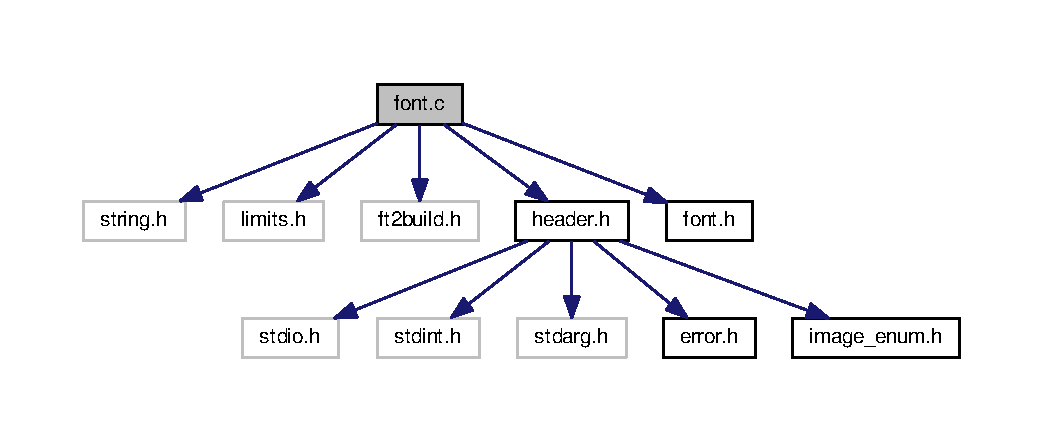
\includegraphics[width=350pt]{font_8c__incl}
\end{center}
\end{figure}
\subsection*{Functions}
\begin{DoxyCompactItemize}
\item 
void \hyperlink{font_8c_a4d66f474b22ed57e551e1c03b08baafe}{imel\+\_\+font\+\_\+write\+\_\+string} (\hyperlink{header_8h_ad8298d38a89742ed84029b278c6acee5}{Imel\+Image} $\ast$image, \hyperlink{header_8h_af8a2b40c34eeed326846d0098ea84ec2}{Imel\+Size} x, \hyperlink{header_8h_af8a2b40c34eeed326846d0098ea84ec2}{Imel\+Size} y, const char $\ast$string, \hyperlink{header_8h_af8a2b40c34eeed326846d0098ea84ec2}{Imel\+Size} px, \hyperlink{header_8h_add7dd9f8c093208bc4fd135a22a670ba}{Imel\+Pixel} pixel)
\begin{DoxyCompactList}\small\item\em Write a string with the internal font. \end{DoxyCompactList}\item 
void \hyperlink{font_8c_a300099d0629f76d81f9e86ce1e5ef73a}{imel\+\_\+font\+\_\+write\+\_\+vstring} (\hyperlink{header_8h_ad8298d38a89742ed84029b278c6acee5}{Imel\+Image} $\ast$image, \hyperlink{header_8h_af8a2b40c34eeed326846d0098ea84ec2}{Imel\+Size} x, \hyperlink{header_8h_af8a2b40c34eeed326846d0098ea84ec2}{Imel\+Size} y, const char $\ast$string, \hyperlink{header_8h_af8a2b40c34eeed326846d0098ea84ec2}{Imel\+Size} px, \hyperlink{header_8h_add7dd9f8c093208bc4fd135a22a670ba}{Imel\+Pixel} pixel)
\begin{DoxyCompactList}\small\item\em Write a string in vertical orientation with the internal font. \end{DoxyCompactList}\item 
\hyperlink{header_8h_a669b28ed18156f1a4f13732e070d6cf2}{bool} \hyperlink{font_8c_a7ca9c7ed1d389c2964ed803332486ef8}{imel\+\_\+font\+\_\+write\+\_\+string\+\_\+with\+\_\+truetype\+\_\+font} (\hyperlink{header_8h_ad8298d38a89742ed84029b278c6acee5}{Imel\+Image} $\ast$$\ast$image, char $\ast$ttf\+\_\+file, \hyperlink{header_8h_af8a2b40c34eeed326846d0098ea84ec2}{Imel\+Size} \+\_\+x, \hyperlink{header_8h_af8a2b40c34eeed326846d0098ea84ec2}{Imel\+Size} y, char $\ast$string, \hyperlink{header_8h_af8a2b40c34eeed326846d0098ea84ec2}{Imel\+Size} px, \hyperlink{header_8h_add7dd9f8c093208bc4fd135a22a670ba}{Imel\+Pixel} pixel,...)
\begin{DoxyCompactList}\small\item\em Write a string with a truetype font. \end{DoxyCompactList}\item 
\hyperlink{header_8h_a669b28ed18156f1a4f13732e070d6cf2}{bool} \hyperlink{font_8c_ac4d01e8c82c3af93d5303e0ca861d662}{imel\+\_\+font\+\_\+write\+\_\+vstring\+\_\+with\+\_\+truetype\+\_\+font} (\hyperlink{header_8h_ad8298d38a89742ed84029b278c6acee5}{Imel\+Image} $\ast$$\ast$image, char $\ast$ttf\+\_\+file, \hyperlink{header_8h_af8a2b40c34eeed326846d0098ea84ec2}{Imel\+Size} \+\_\+x, \hyperlink{header_8h_af8a2b40c34eeed326846d0098ea84ec2}{Imel\+Size} y, char $\ast$string, \hyperlink{header_8h_af8a2b40c34eeed326846d0098ea84ec2}{Imel\+Size} px, \hyperlink{header_8h_add7dd9f8c093208bc4fd135a22a670ba}{Imel\+Pixel} pixel,...)
\begin{DoxyCompactList}\small\item\em Write a string in vertical orientation with a truetype font. \end{DoxyCompactList}\end{DoxyCompactItemize}


\subsection{Detailed Description}
This file contains function to use fonts in an image. 

\begin{DoxyAuthor}{Author}
Davide Francesco Merico These functions allow you to write a string with the internal Imel font or with a truetype font loaded.
\end{DoxyAuthor}
\begin{DoxyNote}{Note}
To use a truetype font is used the Free\+Type library. 
\end{DoxyNote}


\subsection{Function Documentation}
\index{font.\+c@{font.\+c}!imel\+\_\+font\+\_\+write\+\_\+string@{imel\+\_\+font\+\_\+write\+\_\+string}}
\index{imel\+\_\+font\+\_\+write\+\_\+string@{imel\+\_\+font\+\_\+write\+\_\+string}!font.\+c@{font.\+c}}
\subsubsection[{\texorpdfstring{imel\+\_\+font\+\_\+write\+\_\+string(\+Imel\+Image $\ast$image, Imel\+Size x, Imel\+Size y, const char $\ast$string, Imel\+Size px, Imel\+Pixel pixel)}{imel_font_write_string(ImelImage *image, ImelSize x, ImelSize y, const char *string, ImelSize px, ImelPixel pixel)}}]{\setlength{\rightskip}{0pt plus 5cm}void imel\+\_\+font\+\_\+write\+\_\+string (
\begin{DoxyParamCaption}
\item[{{\bf Imel\+Image} $\ast$}]{image, }
\item[{{\bf Imel\+Size}}]{x, }
\item[{{\bf Imel\+Size}}]{y, }
\item[{const char $\ast$}]{string, }
\item[{{\bf Imel\+Size}}]{px, }
\item[{{\bf Imel\+Pixel}}]{pixel}
\end{DoxyParamCaption}
)}\hypertarget{font_8c_a4d66f474b22ed57e551e1c03b08baafe}{}\label{font_8c_a4d66f474b22ed57e551e1c03b08baafe}


Write a string with the internal font. 

This function write the {\ttfamily string} in {\ttfamily image} from coordinate $(x,y)$ with a size of {\ttfamily px}.


\begin{DoxyParams}{Parameters}
{\em image} & Image where write the {\ttfamily string} \\
\hline
{\em x} & Start x coordinate \\
\hline
{\em y} & Start y coordinate \\
\hline
{\em string} & String to write in {\ttfamily image} \\
\hline
{\em px} & Font size, can be specified through Imel\+Font\+Size enum. \\
\hline
{\em pixel} & Color and level of the string \\
\hline
\end{DoxyParams}
\begin{DoxySeeAlso}{See also}
\hyperlink{header_8h_a6d4b2e3b4cd24301c1cf501e73176eed}{Imel\+Font\+Size} 
\end{DoxySeeAlso}
\index{font.\+c@{font.\+c}!imel\+\_\+font\+\_\+write\+\_\+string\+\_\+with\+\_\+truetype\+\_\+font@{imel\+\_\+font\+\_\+write\+\_\+string\+\_\+with\+\_\+truetype\+\_\+font}}
\index{imel\+\_\+font\+\_\+write\+\_\+string\+\_\+with\+\_\+truetype\+\_\+font@{imel\+\_\+font\+\_\+write\+\_\+string\+\_\+with\+\_\+truetype\+\_\+font}!font.\+c@{font.\+c}}
\subsubsection[{\texorpdfstring{imel\+\_\+font\+\_\+write\+\_\+string\+\_\+with\+\_\+truetype\+\_\+font(\+Imel\+Image $\ast$$\ast$image, char $\ast$ttf\+\_\+file, Imel\+Size \+\_\+x, Imel\+Size y, char $\ast$string, Imel\+Size px, Imel\+Pixel pixel,...)}{imel_font_write_string_with_truetype_font(ImelImage **image, char *ttf_file, ImelSize _x, ImelSize y, char *string, ImelSize px, ImelPixel pixel,...)}}]{\setlength{\rightskip}{0pt plus 5cm}{\bf bool} imel\+\_\+font\+\_\+write\+\_\+string\+\_\+with\+\_\+truetype\+\_\+font (
\begin{DoxyParamCaption}
\item[{{\bf Imel\+Image} $\ast$$\ast$}]{image, }
\item[{char $\ast$}]{ttf\+\_\+file, }
\item[{{\bf Imel\+Size}}]{\+\_\+x, }
\item[{{\bf Imel\+Size}}]{y, }
\item[{char $\ast$}]{string, }
\item[{{\bf Imel\+Size}}]{px, }
\item[{{\bf Imel\+Pixel}}]{pixel, }
\item[{}]{...}
\end{DoxyParamCaption}
)}\hypertarget{font_8c_a7ca9c7ed1d389c2964ed803332486ef8}{}\label{font_8c_a7ca9c7ed1d389c2964ed803332486ef8}


Write a string with a truetype font. 

This function write the {\ttfamily string} in {\ttfamily image} from coordinate $(\_x,\_y)$ with a size of {\ttfamily px}.


\begin{DoxyParams}{Parameters}
{\em image} & Image, where write the {\ttfamily string}, passed by address \\
\hline
{\em ttf\+\_\+file} & True\+Type font file name \\
\hline
{\em \+\_\+x} & Start x coordinate \\
\hline
{\em y} & Start y coordinate \\
\hline
{\em string} & String to write in {\ttfamily image} \\
\hline
{\em px} & Font size \\
\hline
{\em pixel} & Color and level of the string \\
\hline
{\em ...} & Additional parameters are characterized by a string and a value. \\
\hline
\end{DoxyParams}
\begin{DoxyNote}{Note}
The string for last parameter are \char`\"{}render-\/type\char`\"{} and \char`\"{}charmap\char`\"{} for the possibily value check the link below. 
\end{DoxyNote}
\begin{DoxySeeAlso}{See also}
\href{http://www.freetype.org/freetype2/docs/reference/ft2-base_interface.html#FT_Render_Mode}{\tt http\+://www.\+freetype.\+org/freetype2/docs/reference/ft2-\/base\+\_\+interface.\+html\#\+F\+T\+\_\+\+Render\+\_\+\+Mode} 

\href{http://www.freetype.org/freetype2/docs/reference/ft2-base_interface.html#FT_Encoding}{\tt http\+://www.\+freetype.\+org/freetype2/docs/reference/ft2-\/base\+\_\+interface.\+html\#\+F\+T\+\_\+\+Encoding} 
\end{DoxySeeAlso}
\index{font.\+c@{font.\+c}!imel\+\_\+font\+\_\+write\+\_\+vstring@{imel\+\_\+font\+\_\+write\+\_\+vstring}}
\index{imel\+\_\+font\+\_\+write\+\_\+vstring@{imel\+\_\+font\+\_\+write\+\_\+vstring}!font.\+c@{font.\+c}}
\subsubsection[{\texorpdfstring{imel\+\_\+font\+\_\+write\+\_\+vstring(\+Imel\+Image $\ast$image, Imel\+Size x, Imel\+Size y, const char $\ast$string, Imel\+Size px, Imel\+Pixel pixel)}{imel_font_write_vstring(ImelImage *image, ImelSize x, ImelSize y, const char *string, ImelSize px, ImelPixel pixel)}}]{\setlength{\rightskip}{0pt plus 5cm}void imel\+\_\+font\+\_\+write\+\_\+vstring (
\begin{DoxyParamCaption}
\item[{{\bf Imel\+Image} $\ast$}]{image, }
\item[{{\bf Imel\+Size}}]{x, }
\item[{{\bf Imel\+Size}}]{y, }
\item[{const char $\ast$}]{string, }
\item[{{\bf Imel\+Size}}]{px, }
\item[{{\bf Imel\+Pixel}}]{pixel}
\end{DoxyParamCaption}
)}\hypertarget{font_8c_a300099d0629f76d81f9e86ce1e5ef73a}{}\label{font_8c_a300099d0629f76d81f9e86ce1e5ef73a}


Write a string in vertical orientation with the internal font. 

This function write the {\ttfamily string} in {\ttfamily image} from coordinate $(x,y)$ with a size of {\ttfamily px}.


\begin{DoxyParams}{Parameters}
{\em image} & Image where write the {\ttfamily string} \\
\hline
{\em x} & Start x coordinate \\
\hline
{\em y} & Start y coordinate \\
\hline
{\em string} & String to write in {\ttfamily image} \\
\hline
{\em px} & Font size, can be specified through Imel\+Font\+Size enum. \\
\hline
{\em pixel} & Color and level of the string \\
\hline
\end{DoxyParams}
\begin{DoxySeeAlso}{See also}
\hyperlink{header_8h_a6d4b2e3b4cd24301c1cf501e73176eed}{Imel\+Font\+Size} 
\end{DoxySeeAlso}
\index{font.\+c@{font.\+c}!imel\+\_\+font\+\_\+write\+\_\+vstring\+\_\+with\+\_\+truetype\+\_\+font@{imel\+\_\+font\+\_\+write\+\_\+vstring\+\_\+with\+\_\+truetype\+\_\+font}}
\index{imel\+\_\+font\+\_\+write\+\_\+vstring\+\_\+with\+\_\+truetype\+\_\+font@{imel\+\_\+font\+\_\+write\+\_\+vstring\+\_\+with\+\_\+truetype\+\_\+font}!font.\+c@{font.\+c}}
\subsubsection[{\texorpdfstring{imel\+\_\+font\+\_\+write\+\_\+vstring\+\_\+with\+\_\+truetype\+\_\+font(\+Imel\+Image $\ast$$\ast$image, char $\ast$ttf\+\_\+file, Imel\+Size \+\_\+x, Imel\+Size y, char $\ast$string, Imel\+Size px, Imel\+Pixel pixel,...)}{imel_font_write_vstring_with_truetype_font(ImelImage **image, char *ttf_file, ImelSize _x, ImelSize y, char *string, ImelSize px, ImelPixel pixel,...)}}]{\setlength{\rightskip}{0pt plus 5cm}{\bf bool} imel\+\_\+font\+\_\+write\+\_\+vstring\+\_\+with\+\_\+truetype\+\_\+font (
\begin{DoxyParamCaption}
\item[{{\bf Imel\+Image} $\ast$$\ast$}]{image, }
\item[{char $\ast$}]{ttf\+\_\+file, }
\item[{{\bf Imel\+Size}}]{\+\_\+x, }
\item[{{\bf Imel\+Size}}]{y, }
\item[{char $\ast$}]{string, }
\item[{{\bf Imel\+Size}}]{px, }
\item[{{\bf Imel\+Pixel}}]{pixel, }
\item[{}]{...}
\end{DoxyParamCaption}
)}\hypertarget{font_8c_ac4d01e8c82c3af93d5303e0ca861d662}{}\label{font_8c_ac4d01e8c82c3af93d5303e0ca861d662}


Write a string in vertical orientation with a truetype font. 

This function write the {\ttfamily string} in {\ttfamily image} from coordinate $(\_x,\_y)$ with a size of {\ttfamily px}.


\begin{DoxyParams}{Parameters}
{\em image} & Image, where write the {\ttfamily string}, passed by address \\
\hline
{\em ttf\+\_\+file} & True\+Type font file name \\
\hline
{\em \+\_\+x} & Start x coordinate \\
\hline
{\em y} & Start y coordinate \\
\hline
{\em string} & String to write in {\ttfamily image} \\
\hline
{\em px} & Font size \\
\hline
{\em pixel} & Color and level of the string \\
\hline
{\em ...} & Additional parameters are characterized by a string and a value. \\
\hline
\end{DoxyParams}
\begin{DoxyNote}{Note}
The string for last parameter are \char`\"{}render-\/type\char`\"{} and \char`\"{}charmap\char`\"{} for the possibily value check the link below. 
\end{DoxyNote}
\begin{DoxySeeAlso}{See also}
\href{http://www.freetype.org/freetype2/docs/reference/ft2-base_interface.html#FT_Render_Mode}{\tt http\+://www.\+freetype.\+org/freetype2/docs/reference/ft2-\/base\+\_\+interface.\+html\#\+F\+T\+\_\+\+Render\+\_\+\+Mode} 

\href{http://www.freetype.org/freetype2/docs/reference/ft2-base_interface.html#FT_Encoding}{\tt http\+://www.\+freetype.\+org/freetype2/docs/reference/ft2-\/base\+\_\+interface.\+html\#\+F\+T\+\_\+\+Encoding} 
\end{DoxySeeAlso}

\hypertarget{font_8h}{}\section{font.\+h File Reference}
\label{font_8h}\index{font.\+h@{font.\+h}}


This file contains the internal Imel font.  


This graph shows which files directly or indirectly include this file\+:
\nopagebreak
\begin{figure}[H]
\begin{center}
\leavevmode
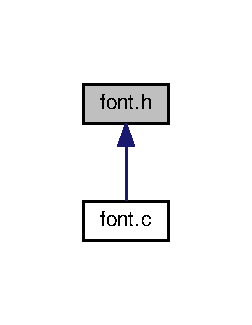
\includegraphics[width=121pt]{font_8h__dep__incl}
\end{center}
\end{figure}
\subsection*{Variables}
\begin{DoxyCompactItemize}
\item 
\hyperlink{header_8h_a669b28ed18156f1a4f13732e070d6cf2}{bool} \hyperlink{font_8h_a2144d898640c91040c731f9353b1e9a2}{imel\+\_\+font} \mbox{[}95\mbox{]}\mbox{[}14\mbox{]}\mbox{[}7\mbox{]}
\end{DoxyCompactItemize}


\subsection{Detailed Description}
This file contains the internal Imel font. 

\begin{DoxyAuthor}{Author}
Davide Francesco Merico 
\end{DoxyAuthor}


\subsection{Variable Documentation}
\index{font.\+h@{font.\+h}!imel\+\_\+font@{imel\+\_\+font}}
\index{imel\+\_\+font@{imel\+\_\+font}!font.\+h@{font.\+h}}
\subsubsection[{\texorpdfstring{imel\+\_\+font}{imel_font}}]{\setlength{\rightskip}{0pt plus 5cm}{\bf bool} imel\+\_\+font\mbox{[}95\mbox{]}\mbox{[}14\mbox{]}\mbox{[}7\mbox{]}}\hypertarget{font_8h_a2144d898640c91040c731f9353b1e9a2}{}\label{font_8h_a2144d898640c91040c731f9353b1e9a2}
Internal font, each letter is 7 px $\ast$ 14 px. There are all printable digit. 
\hypertarget{freetype__export__types_8h}{}\section{freetype\+\_\+export\+\_\+types.\+h File Reference}
\label{freetype__export__types_8h}\index{freetype\+\_\+export\+\_\+types.\+h@{freetype\+\_\+export\+\_\+types.\+h}}


This file contains macro and type for the Free\+Type library.  




\subsection{Detailed Description}
This file contains macro and type for the Free\+Type library. 

\begin{DoxyAuthor}{Author}
Davide Francesco Merico 
\end{DoxyAuthor}

\hypertarget{header_8h}{}\section{header.\+h File Reference}
\label{header_8h}\index{header.\+h@{header.\+h}}


This file contains types and macros used by Imel library.  


{\ttfamily \#include $<$stdio.\+h$>$}\\*
{\ttfamily \#include $<$stdint.\+h$>$}\\*
{\ttfamily \#include $<$stdarg.\+h$>$}\\*
{\ttfamily \#include \char`\"{}error.\+h\char`\"{}}\\*
{\ttfamily \#include \char`\"{}image\+\_\+enum.\+h\char`\"{}}\\*
Include dependency graph for header.\+h\+:
\nopagebreak
\begin{figure}[H]
\begin{center}
\leavevmode
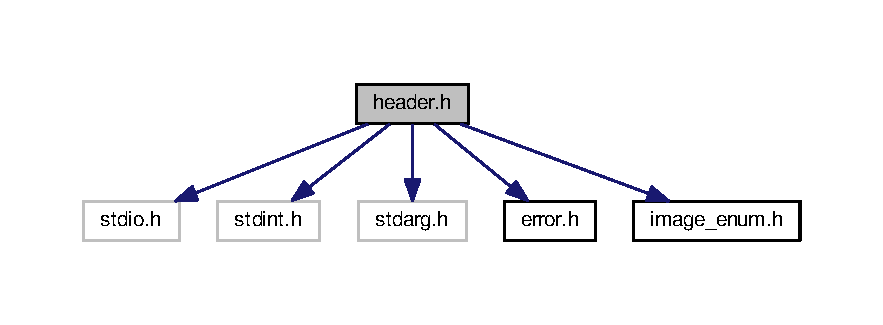
\includegraphics[width=350pt]{header_8h__incl}
\end{center}
\end{figure}
This graph shows which files directly or indirectly include this file\+:
\nopagebreak
\begin{figure}[H]
\begin{center}
\leavevmode
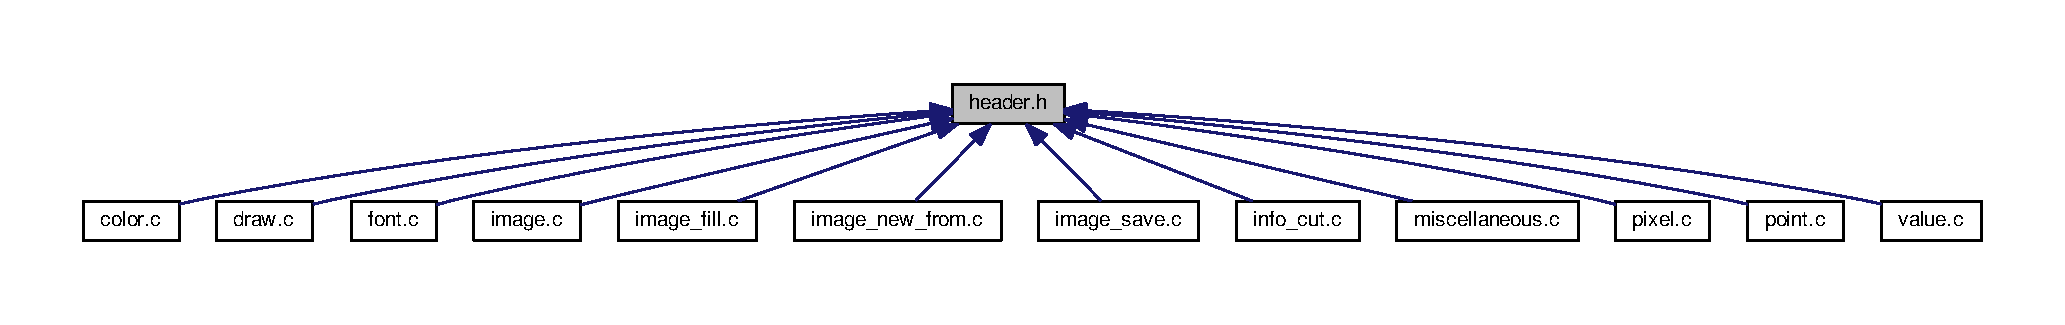
\includegraphics[width=350pt]{header_8h__dep__incl}
\end{center}
\end{figure}
\subsection*{Data Structures}
\begin{DoxyCompactItemize}
\item 
struct \hyperlink{struct__imel__pixel}{\+\_\+imel\+\_\+pixel}
\begin{DoxyCompactList}\small\item\em Rappresentation of a pixel in Imel library. \end{DoxyCompactList}\item 
struct \hyperlink{struct__imel__image}{\+\_\+imel\+\_\+image}
\begin{DoxyCompactList}\small\item\em Rappresentation of an image in Imel library. \end{DoxyCompactList}\item 
struct \hyperlink{struct__imel__point}{\+\_\+imel\+\_\+point}
\begin{DoxyCompactList}\small\item\em Rappresentation of a point in Imel library. \end{DoxyCompactList}\item 
struct \hyperlink{struct__imel__error}{\+\_\+imel\+\_\+error}
\begin{DoxyCompactList}\small\item\em Specialized type in reporting errors inside Imel. \end{DoxyCompactList}\item 
struct \hyperlink{struct__imel__info__cut}{\+\_\+imel\+\_\+info\+\_\+cut}
\item 
struct \hyperlink{struct__imel__hsl}{\+\_\+imel\+\_\+hsl}
\end{DoxyCompactItemize}
\subsection*{Macros}
\begin{DoxyCompactItemize}
\item 
\#define \hyperlink{header_8h_a2ae0a8abf6869d91ed8f6847fb3b014d}{I\+M\+E\+L\+\_\+\+V\+E\+R\+S\+I\+O\+N\+\_\+\+M\+A\+J\+OR}~3
\item 
\#define \hyperlink{header_8h_ac4bb99e092c40c1a0519fd1b9d538d82}{I\+M\+E\+L\+\_\+\+V\+E\+R\+S\+I\+O\+N\+\_\+\+M\+I\+N\+OR}~0
\item 
\#define \hyperlink{header_8h_a2505069f13628a303bdf360de2d8490f}{R\+G\+B\+A\+\_\+\+R\+\_\+\+M\+A\+SK}(val)~(((val) \& 0xff000000) $>$$>$ 24)
\item 
\#define \hyperlink{header_8h_a632c40a96aac3972b668bb536fb1af06}{R\+G\+B\+A\+\_\+\+G\+\_\+\+M\+A\+SK}(val)~(((val) \& 0xff0000) $>$$>$ 16)
\item 
\#define \hyperlink{header_8h_ade6c182c68e6a0a7638eb05a6143f3f0}{R\+G\+B\+A\+\_\+\+B\+\_\+\+M\+A\+SK}(val)~(((val) \& 0xff00) $>$$>$ 8)
\item 
\#define \hyperlink{header_8h_ac837716be1eb4f0071c03b7b4b4fb2b0}{R\+G\+B\+A\+\_\+\+A\+\_\+\+M\+A\+SK}(val)~((val) \& 0xff)
\item 
\#define \hyperlink{header_8h_a0978c9c7420f81adda347a7c6d22f085}{D\+E\+G\+\_\+\+T\+O\+\_\+\+R\+AD}(val)~(0.\+017453292 $\ast$ (val))
\item 
\#define \hyperlink{header_8h_adff9f86a929b90364f856932fc5e064f}{R\+A\+D\+\_\+\+T\+O\+\_\+\+D\+EG}(val)~(57.\+29577951 $\ast$ (val))
\item 
\#define \hyperlink{header_8h_aedf541d4162f35857638d2ececedc2d7}{return\+\_\+var\+\_\+if\+\_\+fail}(condition,  var)
\item 
\#define \hyperlink{header_8h_afa6c4a6400518363dd86d406785585b2}{return\+\_\+if\+\_\+fail}(condition)
\end{DoxyCompactItemize}
\subsection*{Typedefs}
\begin{DoxyCompactItemize}
\item 
typedef enum \+\_\+bool\+\_\+type \hyperlink{header_8h_a669b28ed18156f1a4f13732e070d6cf2}{bool}
\item 
typedef uint32\+\_\+t \hyperlink{header_8h_af8a2b40c34eeed326846d0098ea84ec2}{Imel\+Size}
\item 
typedef uint8\+\_\+t \hyperlink{header_8h_add1326f75f0c1a7da9f14c2ed4f673e9}{Imel\+Color}
\item 
typedef int32\+\_\+t \hyperlink{header_8h_a97bc4b146a807c2d83b966983132f4fc}{Imel\+Level}
\item 
typedef enum \hyperlink{header_8h_a765ae01cc88c760f3df918af6fd4943c}{\+\_\+imel\+\_\+effect} \hyperlink{header_8h_a4919a9d01ef8388db452c59507d67f2e}{Imel\+Effect}
\item 
typedef enum \hyperlink{header_8h_a5a8e15aebc9573a522ef1d8eb86bac6e}{\+\_\+imel\+\_\+mask} \hyperlink{header_8h_a9facf73fdf3eb7434d01cd1c07341a28}{Imel\+Mask}
\item 
typedef enum \hyperlink{header_8h_a9f975dccb73dc4b4f6f137cd80fc1387}{\+\_\+imel\+\_\+logic\+\_\+operation} \hyperlink{header_8h_af92bba14d49d8e59b2642eb300fedb5e}{Imel\+Logic\+Operation}
\item 
typedef enum \hyperlink{header_8h_abc4cf7641abd06646b239f69f7800e37}{\+\_\+imel\+\_\+font\+\_\+size} \hyperlink{header_8h_a6d4b2e3b4cd24301c1cf501e73176eed}{Imel\+Font\+Size}
\item 
typedef enum \hyperlink{header_8h_ace9df0e53e30f77ba713148ea7b106a8}{\+\_\+imel\+\_\+histogram} \hyperlink{header_8h_a8879c5e403ddb26c326b1cc2c3e529bf}{Imel\+Histogram}
\item 
typedef enum \hyperlink{header_8h_af6c0ec142c15baf126c12fbd5c57f322}{\+\_\+imel\+\_\+histogram\+\_\+layout} \hyperlink{header_8h_aacf376be43512b219081df71ed7ee438}{Imel\+Histogram\+Layout}
\item 
typedef enum \hyperlink{header_8h_a2165f253ebc3e84d406c905ab1d77e7f}{\+\_\+imel\+\_\+orientation} \hyperlink{header_8h_aef27fcac7a96d118b3c3194c2577049f}{Imel\+Orientation}
\item 
typedef enum \hyperlink{header_8h_a07a69c435daa766b8e1b6962f0956202}{\+\_\+imel\+\_\+level\+\_\+operation} \hyperlink{header_8h_abece8958e8db1e2826f21fd822c14694}{Imel\+Level\+Operation}
\item 
typedef enum \hyperlink{header_8h_aacc3beb92f2372f7d6ae2a9f8de1a567}{\+\_\+imel\+\_\+noise\+\_\+operation} \hyperlink{header_8h_abb411905768327b93668c636957a73ff}{Imel\+Noise\+Operation}
\item 
typedef enum \hyperlink{header_8h_a191ba3a796907e762b75b21308992809}{\+\_\+imel\+\_\+pattern\+\_\+operation} \hyperlink{header_8h_a7321d084db08c3a51089e8a4612b332b}{Imel\+Pattern\+Operation}
\item 
typedef enum \hyperlink{header_8h_aaf7d1762a05a9d183fd8b718cbb2d338}{\+\_\+imel\+\_\+alignment} \hyperlink{header_8h_a4d620b3c547205ca76d92f43f09320d1}{Imel\+Alignment}
\item 
typedef enum \hyperlink{header_8h_ad11ee694d9812e135c152f4623da3452}{\+\_\+imel\+\_\+ref} \hyperlink{header_8h_a6182c8947d12d828155f0fb8cb024209}{Imel\+Ref}
\item 
typedef enum \hyperlink{header_8h_aa326347c06714f71ccc11ba6eea7a08a}{\+\_\+imel\+\_\+value} \hyperlink{header_8h_a3b961ca2b6e1029ab77a0951c3ae7260}{Imel\+Value}
\item 
typedef struct \hyperlink{struct__imel__pixel}{\+\_\+imel\+\_\+pixel} \hyperlink{header_8h_add7dd9f8c093208bc4fd135a22a670ba}{Imel\+Pixel}
\begin{DoxyCompactList}\small\item\em Rappresentation of a pixel in Imel library. \end{DoxyCompactList}\item 
typedef struct \hyperlink{struct__imel__image}{\+\_\+imel\+\_\+image} \hyperlink{header_8h_ad8298d38a89742ed84029b278c6acee5}{Imel\+Image}
\begin{DoxyCompactList}\small\item\em Rappresentation of an image in Imel library. \end{DoxyCompactList}\item 
typedef struct \hyperlink{struct__imel__point}{\+\_\+imel\+\_\+point} \hyperlink{header_8h_a8b81d020f830e116585b833ea21410c1}{Imel\+Point}
\begin{DoxyCompactList}\small\item\em Rappresentation of a point in Imel library. \end{DoxyCompactList}\item 
typedef struct \hyperlink{struct__imel__error}{\+\_\+imel\+\_\+error} \hyperlink{header_8h_abe31dcaa4b6683d315101c48b1ca2a56}{Imel\+Error}
\begin{DoxyCompactList}\small\item\em Specialized type in reporting errors inside Imel. \end{DoxyCompactList}\item 
typedef struct \hyperlink{struct__imel__info__cut}{\+\_\+imel\+\_\+info\+\_\+cut} \hyperlink{header_8h_a3f4de920943cb4d0979d415b4c5e3989}{Imel\+Info\+Cut}
\item 
typedef struct \hyperlink{struct__imel__hsl}{\+\_\+imel\+\_\+hsl} \hyperlink{header_8h_a851541a4411924d91d8abd55939c3b23}{Imel\+H\+SL}
\item 
typedef \hyperlink{header_8h_ad8298d38a89742ed84029b278c6acee5}{Imel\+Image} $\ast$ \hyperlink{header_8h_aaa14cf408b64a8162fd57c4b4c081e1a}{Imel\+Image\+Ptr}
\item 
typedef void $\ast$ \hyperlink{header_8h_a0a9244570c47547d00bfba1bb77d70f1}{Imel\+Generic\+Ptr}
\item 
typedef void($\ast$ \hyperlink{header_8h_afae32b8dba9014bfbe4456e85ddbb9ac}{Imel\+Generic\+Func\+Ptr}) (\hyperlink{header_8h_aaa14cf408b64a8162fd57c4b4c081e1a}{Imel\+Image\+Ptr}, \hyperlink{header_8h_a0a9244570c47547d00bfba1bb77d70f1}{Imel\+Generic\+Ptr})
\end{DoxyCompactItemize}
\subsection*{Enumerations}
\subsection*{Functions}
\begin{DoxyCompactItemize}
\item 
\hyperlink{header_8h_a669b28ed18156f1a4f13732e070d6cf2}{bool} \hyperlink{header_8h_ad4629c597b8f8827434c9ca3b183c4de}{imel\+\_\+printf\+\_\+debug} (const char $\ast$function, const char $\ast$filename, const char $\ast$error\+\_\+level, char $\ast$\+\_\+\+\_\+format,...)
\end{DoxyCompactItemize}


\subsection{Detailed Description}
This file contains types and macros used by Imel library. 

\begin{DoxyAuthor}{Author}
Davide Francesco Merico 
\end{DoxyAuthor}


\subsection{Macro Definition Documentation}
\index{header.\+h@{header.\+h}!D\+E\+G\+\_\+\+T\+O\+\_\+\+R\+AD@{D\+E\+G\+\_\+\+T\+O\+\_\+\+R\+AD}}
\index{D\+E\+G\+\_\+\+T\+O\+\_\+\+R\+AD@{D\+E\+G\+\_\+\+T\+O\+\_\+\+R\+AD}!header.\+h@{header.\+h}}
\subsubsection[{\texorpdfstring{D\+E\+G\+\_\+\+T\+O\+\_\+\+R\+AD}{DEG_TO_RAD}}]{\setlength{\rightskip}{0pt plus 5cm}\#define D\+E\+G\+\_\+\+T\+O\+\_\+\+R\+AD(
\begin{DoxyParamCaption}
\item[{}]{val}
\end{DoxyParamCaption}
)~(0.\+017453292 $\ast$ (val))}\hypertarget{header_8h_a0978c9c7420f81adda347a7c6d22f085}{}\label{header_8h_a0978c9c7420f81adda347a7c6d22f085}
Convert degrees to radians \index{header.\+h@{header.\+h}!I\+M\+E\+L\+\_\+\+V\+E\+R\+S\+I\+O\+N\+\_\+\+M\+A\+J\+OR@{I\+M\+E\+L\+\_\+\+V\+E\+R\+S\+I\+O\+N\+\_\+\+M\+A\+J\+OR}}
\index{I\+M\+E\+L\+\_\+\+V\+E\+R\+S\+I\+O\+N\+\_\+\+M\+A\+J\+OR@{I\+M\+E\+L\+\_\+\+V\+E\+R\+S\+I\+O\+N\+\_\+\+M\+A\+J\+OR}!header.\+h@{header.\+h}}
\subsubsection[{\texorpdfstring{I\+M\+E\+L\+\_\+\+V\+E\+R\+S\+I\+O\+N\+\_\+\+M\+A\+J\+OR}{IMEL_VERSION_MAJOR}}]{\setlength{\rightskip}{0pt plus 5cm}\#define I\+M\+E\+L\+\_\+\+V\+E\+R\+S\+I\+O\+N\+\_\+\+M\+A\+J\+OR~3}\hypertarget{header_8h_a2ae0a8abf6869d91ed8f6847fb3b014d}{}\label{header_8h_a2ae0a8abf6869d91ed8f6847fb3b014d}
Imel version major \index{header.\+h@{header.\+h}!I\+M\+E\+L\+\_\+\+V\+E\+R\+S\+I\+O\+N\+\_\+\+M\+I\+N\+OR@{I\+M\+E\+L\+\_\+\+V\+E\+R\+S\+I\+O\+N\+\_\+\+M\+I\+N\+OR}}
\index{I\+M\+E\+L\+\_\+\+V\+E\+R\+S\+I\+O\+N\+\_\+\+M\+I\+N\+OR@{I\+M\+E\+L\+\_\+\+V\+E\+R\+S\+I\+O\+N\+\_\+\+M\+I\+N\+OR}!header.\+h@{header.\+h}}
\subsubsection[{\texorpdfstring{I\+M\+E\+L\+\_\+\+V\+E\+R\+S\+I\+O\+N\+\_\+\+M\+I\+N\+OR}{IMEL_VERSION_MINOR}}]{\setlength{\rightskip}{0pt plus 5cm}\#define I\+M\+E\+L\+\_\+\+V\+E\+R\+S\+I\+O\+N\+\_\+\+M\+I\+N\+OR~0}\hypertarget{header_8h_ac4bb99e092c40c1a0519fd1b9d538d82}{}\label{header_8h_ac4bb99e092c40c1a0519fd1b9d538d82}
Imel version minor \index{header.\+h@{header.\+h}!R\+A\+D\+\_\+\+T\+O\+\_\+\+D\+EG@{R\+A\+D\+\_\+\+T\+O\+\_\+\+D\+EG}}
\index{R\+A\+D\+\_\+\+T\+O\+\_\+\+D\+EG@{R\+A\+D\+\_\+\+T\+O\+\_\+\+D\+EG}!header.\+h@{header.\+h}}
\subsubsection[{\texorpdfstring{R\+A\+D\+\_\+\+T\+O\+\_\+\+D\+EG}{RAD_TO_DEG}}]{\setlength{\rightskip}{0pt plus 5cm}\#define R\+A\+D\+\_\+\+T\+O\+\_\+\+D\+EG(
\begin{DoxyParamCaption}
\item[{}]{val}
\end{DoxyParamCaption}
)~(57.\+29577951 $\ast$ (val))}\hypertarget{header_8h_adff9f86a929b90364f856932fc5e064f}{}\label{header_8h_adff9f86a929b90364f856932fc5e064f}
Convert radians to degrees \index{header.\+h@{header.\+h}!return\+\_\+if\+\_\+fail@{return\+\_\+if\+\_\+fail}}
\index{return\+\_\+if\+\_\+fail@{return\+\_\+if\+\_\+fail}!header.\+h@{header.\+h}}
\subsubsection[{\texorpdfstring{return\+\_\+if\+\_\+fail}{return_if_fail}}]{\setlength{\rightskip}{0pt plus 5cm}\#define return\+\_\+if\+\_\+fail(
\begin{DoxyParamCaption}
\item[{}]{condition}
\end{DoxyParamCaption}
)}\hypertarget{header_8h_afa6c4a6400518363dd86d406785585b2}{}\label{header_8h_afa6c4a6400518363dd86d406785585b2}
{\bfseries Value\+:}
\begin{DoxyCode}
\textcolor{keywordflow}{if} ( !(condition) ) \{ \hyperlink{header_8h_ad4629c597b8f8827434c9ca3b183c4de}{\(\backslash\)}
\hyperlink{header_8h_ad4629c597b8f8827434c9ca3b183c4de}{             imel\_printf\_debug} (NULL, NULL, \textcolor{stringliteral}{"warning"}, \textcolor{stringliteral}{"condition failed.\(\backslash\)n"})
      ; \(\backslash\)
             return; \(\backslash\)
        \}
\end{DoxyCode}
Return if {\ttfamily condition} is T\+R\+UE \index{header.\+h@{header.\+h}!return\+\_\+var\+\_\+if\+\_\+fail@{return\+\_\+var\+\_\+if\+\_\+fail}}
\index{return\+\_\+var\+\_\+if\+\_\+fail@{return\+\_\+var\+\_\+if\+\_\+fail}!header.\+h@{header.\+h}}
\subsubsection[{\texorpdfstring{return\+\_\+var\+\_\+if\+\_\+fail}{return_var_if_fail}}]{\setlength{\rightskip}{0pt plus 5cm}\#define return\+\_\+var\+\_\+if\+\_\+fail(
\begin{DoxyParamCaption}
\item[{}]{condition, }
\item[{}]{var}
\end{DoxyParamCaption}
)}\hypertarget{header_8h_aedf541d4162f35857638d2ececedc2d7}{}\label{header_8h_aedf541d4162f35857638d2ececedc2d7}
{\bfseries Value\+:}
\begin{DoxyCode}
\textcolor{keywordflow}{if} ( !(condition) ) \{ \hyperlink{header_8h_ad4629c597b8f8827434c9ca3b183c4de}{\(\backslash\)}
\hyperlink{header_8h_ad4629c597b8f8827434c9ca3b183c4de}{             imel\_printf\_debug} (NULL, NULL, \textcolor{stringliteral}{"warning"}, \textcolor{stringliteral}{"condition failed.\(\backslash\)n"})
      ; \(\backslash\)
             return (var); \(\backslash\)
        \}
\end{DoxyCode}
Return {\ttfamily var} if {\ttfamily condition} is T\+R\+UE \index{header.\+h@{header.\+h}!R\+G\+B\+A\+\_\+\+A\+\_\+\+M\+A\+SK@{R\+G\+B\+A\+\_\+\+A\+\_\+\+M\+A\+SK}}
\index{R\+G\+B\+A\+\_\+\+A\+\_\+\+M\+A\+SK@{R\+G\+B\+A\+\_\+\+A\+\_\+\+M\+A\+SK}!header.\+h@{header.\+h}}
\subsubsection[{\texorpdfstring{R\+G\+B\+A\+\_\+\+A\+\_\+\+M\+A\+SK}{RGBA_A_MASK}}]{\setlength{\rightskip}{0pt plus 5cm}\#define R\+G\+B\+A\+\_\+\+A\+\_\+\+M\+A\+SK(
\begin{DoxyParamCaption}
\item[{}]{val}
\end{DoxyParamCaption}
)~((val) \& 0xff)}\hypertarget{header_8h_ac837716be1eb4f0071c03b7b4b4fb2b0}{}\label{header_8h_ac837716be1eb4f0071c03b7b4b4fb2b0}
Mask for alpha channel in a R\+G\+BA value \index{header.\+h@{header.\+h}!R\+G\+B\+A\+\_\+\+B\+\_\+\+M\+A\+SK@{R\+G\+B\+A\+\_\+\+B\+\_\+\+M\+A\+SK}}
\index{R\+G\+B\+A\+\_\+\+B\+\_\+\+M\+A\+SK@{R\+G\+B\+A\+\_\+\+B\+\_\+\+M\+A\+SK}!header.\+h@{header.\+h}}
\subsubsection[{\texorpdfstring{R\+G\+B\+A\+\_\+\+B\+\_\+\+M\+A\+SK}{RGBA_B_MASK}}]{\setlength{\rightskip}{0pt plus 5cm}\#define R\+G\+B\+A\+\_\+\+B\+\_\+\+M\+A\+SK(
\begin{DoxyParamCaption}
\item[{}]{val}
\end{DoxyParamCaption}
)~(((val) \& 0xff00) $>$$>$ 8)}\hypertarget{header_8h_ade6c182c68e6a0a7638eb05a6143f3f0}{}\label{header_8h_ade6c182c68e6a0a7638eb05a6143f3f0}
Mask for blue channel in a R\+G\+BA value \index{header.\+h@{header.\+h}!R\+G\+B\+A\+\_\+\+G\+\_\+\+M\+A\+SK@{R\+G\+B\+A\+\_\+\+G\+\_\+\+M\+A\+SK}}
\index{R\+G\+B\+A\+\_\+\+G\+\_\+\+M\+A\+SK@{R\+G\+B\+A\+\_\+\+G\+\_\+\+M\+A\+SK}!header.\+h@{header.\+h}}
\subsubsection[{\texorpdfstring{R\+G\+B\+A\+\_\+\+G\+\_\+\+M\+A\+SK}{RGBA_G_MASK}}]{\setlength{\rightskip}{0pt plus 5cm}\#define R\+G\+B\+A\+\_\+\+G\+\_\+\+M\+A\+SK(
\begin{DoxyParamCaption}
\item[{}]{val}
\end{DoxyParamCaption}
)~(((val) \& 0xff0000) $>$$>$ 16)}\hypertarget{header_8h_a632c40a96aac3972b668bb536fb1af06}{}\label{header_8h_a632c40a96aac3972b668bb536fb1af06}
Mask for green channel in a R\+G\+BA value \index{header.\+h@{header.\+h}!R\+G\+B\+A\+\_\+\+R\+\_\+\+M\+A\+SK@{R\+G\+B\+A\+\_\+\+R\+\_\+\+M\+A\+SK}}
\index{R\+G\+B\+A\+\_\+\+R\+\_\+\+M\+A\+SK@{R\+G\+B\+A\+\_\+\+R\+\_\+\+M\+A\+SK}!header.\+h@{header.\+h}}
\subsubsection[{\texorpdfstring{R\+G\+B\+A\+\_\+\+R\+\_\+\+M\+A\+SK}{RGBA_R_MASK}}]{\setlength{\rightskip}{0pt plus 5cm}\#define R\+G\+B\+A\+\_\+\+R\+\_\+\+M\+A\+SK(
\begin{DoxyParamCaption}
\item[{}]{val}
\end{DoxyParamCaption}
)~(((val) \& 0xff000000) $>$$>$ 24)}\hypertarget{header_8h_a2505069f13628a303bdf360de2d8490f}{}\label{header_8h_a2505069f13628a303bdf360de2d8490f}
Mask for red channel in a R\+G\+BA value 

\subsection{Typedef Documentation}
\index{header.\+h@{header.\+h}!bool@{bool}}
\index{bool@{bool}!header.\+h@{header.\+h}}
\subsubsection[{\texorpdfstring{bool}{bool}}]{\setlength{\rightskip}{0pt plus 5cm}typedef enum \+\_\+bool\+\_\+type  {\bf bool}}\hypertarget{header_8h_a669b28ed18156f1a4f13732e070d6cf2}{}\label{header_8h_a669b28ed18156f1a4f13732e070d6cf2}
Boolean type \index{header.\+h@{header.\+h}!Imel\+Alignment@{Imel\+Alignment}}
\index{Imel\+Alignment@{Imel\+Alignment}!header.\+h@{header.\+h}}
\subsubsection[{\texorpdfstring{Imel\+Alignment}{ImelAlignment}}]{\setlength{\rightskip}{0pt plus 5cm}typedef enum {\bf \+\_\+imel\+\_\+alignment}  {\bf Imel\+Alignment}}\hypertarget{header_8h_a4d620b3c547205ca76d92f43f09320d1}{}\label{header_8h_a4d620b3c547205ca76d92f43f09320d1}
Imel\+Alignment type. Specifies the image alignment.

\begin{DoxySeeAlso}{See also}
\hyperlink{image_8c_a12519cad063897a1dcf9eb4c677b8304}{imel\+\_\+image\+\_\+union} 
\end{DoxySeeAlso}
\index{header.\+h@{header.\+h}!Imel\+Color@{Imel\+Color}}
\index{Imel\+Color@{Imel\+Color}!header.\+h@{header.\+h}}
\subsubsection[{\texorpdfstring{Imel\+Color}{ImelColor}}]{\setlength{\rightskip}{0pt plus 5cm}typedef uint8\+\_\+t {\bf Imel\+Color}}\hypertarget{header_8h_add1326f75f0c1a7da9f14c2ed4f673e9}{}\label{header_8h_add1326f75f0c1a7da9f14c2ed4f673e9}
Imel\+Color type \index{header.\+h@{header.\+h}!Imel\+Effect@{Imel\+Effect}}
\index{Imel\+Effect@{Imel\+Effect}!header.\+h@{header.\+h}}
\subsubsection[{\texorpdfstring{Imel\+Effect}{ImelEffect}}]{\setlength{\rightskip}{0pt plus 5cm}typedef enum {\bf \+\_\+imel\+\_\+effect}  {\bf Imel\+Effect}}\hypertarget{header_8h_a4919a9d01ef8388db452c59507d67f2e}{}\label{header_8h_a4919a9d01ef8388db452c59507d67f2e}
Effects to apply through \hyperlink{image_8c_af617e35a65519b8c9c33b49fc8e59e89}{imel\+\_\+image\+\_\+apply\+\_\+effect} or some other function.

\begin{DoxyNote}{Note}
Enum values starts from 0 
\end{DoxyNote}
\begin{DoxySeeAlso}{See also}
\hyperlink{image_8c_af617e35a65519b8c9c33b49fc8e59e89}{imel\+\_\+image\+\_\+apply\+\_\+effect} 
\end{DoxySeeAlso}
\index{header.\+h@{header.\+h}!Imel\+Error@{Imel\+Error}}
\index{Imel\+Error@{Imel\+Error}!header.\+h@{header.\+h}}
\subsubsection[{\texorpdfstring{Imel\+Error}{ImelError}}]{\setlength{\rightskip}{0pt plus 5cm}typedef struct {\bf \+\_\+imel\+\_\+error}  {\bf Imel\+Error}}\hypertarget{header_8h_abe31dcaa4b6683d315101c48b1ca2a56}{}\label{header_8h_abe31dcaa4b6683d315101c48b1ca2a56}


Specialized type in reporting errors inside Imel. 

This type report an error if occurred when doing operations in Imel. Each error have a code and a description.

\begin{DoxyNote}{Note}
Usually it can be used in this way\+: 
\begin{DoxyCode}
1 ImelImage *image;
2 ImelError error;
3 
4 image = imel\_image\_new\_from ("image.png", 0, &error);
5 if ( !image ) \{
6      fprintf (stderr, "Error %d: %s\(\backslash\)n", error.code, error.description);
7      return 1;
8 \}
\end{DoxyCode}
 
\end{DoxyNote}
\index{header.\+h@{header.\+h}!Imel\+Font\+Size@{Imel\+Font\+Size}}
\index{Imel\+Font\+Size@{Imel\+Font\+Size}!header.\+h@{header.\+h}}
\subsubsection[{\texorpdfstring{Imel\+Font\+Size}{ImelFontSize}}]{\setlength{\rightskip}{0pt plus 5cm}typedef enum {\bf \+\_\+imel\+\_\+font\+\_\+size}  {\bf Imel\+Font\+Size}}\hypertarget{header_8h_a6d4b2e3b4cd24301c1cf501e73176eed}{}\label{header_8h_a6d4b2e3b4cd24301c1cf501e73176eed}
Imel\+Font\+Size type. Enumerator created to facilitate the insertion of standard sizes for the internal fonts in Imel whose size is 14px or I\+M\+E\+L\+\_\+\+F\+O\+N\+T\+\_\+\+S\+I\+Z\+E\+\_\+\+M\+E\+D\+I\+UM, other values have been incorporated to avoid as much as possible the presence of artifacts that degrade the image.

\begin{DoxySeeAlso}{See also}
\hyperlink{font_8c_a4d66f474b22ed57e551e1c03b08baafe}{imel\+\_\+font\+\_\+write\+\_\+string} 

\hyperlink{font_8c_a300099d0629f76d81f9e86ce1e5ef73a}{imel\+\_\+font\+\_\+write\+\_\+vstring} 
\end{DoxySeeAlso}
\index{header.\+h@{header.\+h}!Imel\+Generic\+Func\+Ptr@{Imel\+Generic\+Func\+Ptr}}
\index{Imel\+Generic\+Func\+Ptr@{Imel\+Generic\+Func\+Ptr}!header.\+h@{header.\+h}}
\subsubsection[{\texorpdfstring{Imel\+Generic\+Func\+Ptr}{ImelGenericFuncPtr}}]{\setlength{\rightskip}{0pt plus 5cm}typedef void($\ast$ Imel\+Generic\+Func\+Ptr) ({\bf Imel\+Image\+Ptr}, {\bf Imel\+Generic\+Ptr})}\hypertarget{header_8h_afae32b8dba9014bfbe4456e85ddbb9ac}{}\label{header_8h_afae32b8dba9014bfbe4456e85ddbb9ac}
Generic function to operate with image and data. \begin{DoxyNote}{Note}
Used internally. 
\end{DoxyNote}
\index{header.\+h@{header.\+h}!Imel\+Generic\+Ptr@{Imel\+Generic\+Ptr}}
\index{Imel\+Generic\+Ptr@{Imel\+Generic\+Ptr}!header.\+h@{header.\+h}}
\subsubsection[{\texorpdfstring{Imel\+Generic\+Ptr}{ImelGenericPtr}}]{\setlength{\rightskip}{0pt plus 5cm}typedef void$\ast$ {\bf Imel\+Generic\+Ptr}}\hypertarget{header_8h_a0a9244570c47547d00bfba1bb77d70f1}{}\label{header_8h_a0a9244570c47547d00bfba1bb77d70f1}
Generic pointer \begin{DoxyNote}{Note}
Used internally. 
\end{DoxyNote}
\index{header.\+h@{header.\+h}!Imel\+Histogram@{Imel\+Histogram}}
\index{Imel\+Histogram@{Imel\+Histogram}!header.\+h@{header.\+h}}
\subsubsection[{\texorpdfstring{Imel\+Histogram}{ImelHistogram}}]{\setlength{\rightskip}{0pt plus 5cm}typedef enum {\bf \+\_\+imel\+\_\+histogram}  {\bf Imel\+Histogram}}\hypertarget{header_8h_a8879c5e403ddb26c326b1cc2c3e529bf}{}\label{header_8h_a8879c5e403ddb26c326b1cc2c3e529bf}
Imel\+Histogram type. Specifies which histogram to get from an image.

\begin{DoxySeeAlso}{See also}
\hyperlink{image_8c_afa2cd389929358c87f2d21e1e7b2ef9a}{imel\+\_\+image\+\_\+get\+\_\+histogram} 

\hyperlink{image_8c_ae416e85c63ce2f3f60df3fb31c5d41b5}{imel\+\_\+image\+\_\+get\+\_\+histogram\+\_\+image} 
\end{DoxySeeAlso}
\index{header.\+h@{header.\+h}!Imel\+Histogram\+Layout@{Imel\+Histogram\+Layout}}
\index{Imel\+Histogram\+Layout@{Imel\+Histogram\+Layout}!header.\+h@{header.\+h}}
\subsubsection[{\texorpdfstring{Imel\+Histogram\+Layout}{ImelHistogramLayout}}]{\setlength{\rightskip}{0pt plus 5cm}typedef enum {\bf \+\_\+imel\+\_\+histogram\+\_\+layout}  {\bf Imel\+Histogram\+Layout}}\hypertarget{header_8h_aacf376be43512b219081df71ed7ee438}{}\label{header_8h_aacf376be43512b219081df71ed7ee438}
Imelhistogram\+Layout type. Specifies the histogram layout.

\begin{DoxySeeAlso}{See also}
\hyperlink{image_8c_a41cc4f146e4863e1969bfa15ca3e7afc}{imel\+\_\+image\+\_\+get\+\_\+histograms\+\_\+image} 
\end{DoxySeeAlso}
\index{header.\+h@{header.\+h}!Imel\+H\+SL@{Imel\+H\+SL}}
\index{Imel\+H\+SL@{Imel\+H\+SL}!header.\+h@{header.\+h}}
\subsubsection[{\texorpdfstring{Imel\+H\+SL}{ImelHSL}}]{\setlength{\rightskip}{0pt plus 5cm}typedef struct {\bf \+\_\+imel\+\_\+hsl}  {\bf Imel\+H\+SL}}\hypertarget{header_8h_a851541a4411924d91d8abd55939c3b23}{}\label{header_8h_a851541a4411924d91d8abd55939c3b23}
This type can identify a color through H\+SL values.

\begin{DoxySeeAlso}{See also}
\hyperlink{pixel_8c_a8ba2bb2ac90703240cd2c7556a4b9680}{imel\+\_\+pixel\+\_\+new\+\_\+from\+\_\+hsl} 

\hyperlink{pixel_8c_a29873cfd499af84deec32931e77e178e}{imel\+\_\+pixel\+\_\+get\+\_\+hsl} 
\end{DoxySeeAlso}
\index{header.\+h@{header.\+h}!Imel\+Image@{Imel\+Image}}
\index{Imel\+Image@{Imel\+Image}!header.\+h@{header.\+h}}
\subsubsection[{\texorpdfstring{Imel\+Image}{ImelImage}}]{\setlength{\rightskip}{0pt plus 5cm}typedef struct {\bf \+\_\+imel\+\_\+image}  {\bf Imel\+Image}}\hypertarget{header_8h_ad8298d38a89742ed84029b278c6acee5}{}\label{header_8h_ad8298d38a89742ed84029b278c6acee5}


Rappresentation of an image in Imel library. 

The most important type of Imel with \hyperlink{header_8h_add7dd9f8c093208bc4fd135a22a670ba}{Imel\+Pixel} is this. This type, in Imel, is an image which contains its resolution and its colors.

\begin{DoxySeeAlso}{See also}
\hyperlink{image_8c_af3a4abcb52f5611781065536fda0f97e}{imel\+\_\+image\+\_\+new} 

\hyperlink{image__new__from_8c_a43a15b507cf100b80bc07ce92a48adc7}{imel\+\_\+image\+\_\+new\+\_\+from} 
\end{DoxySeeAlso}
\index{header.\+h@{header.\+h}!Imel\+Image\+Ptr@{Imel\+Image\+Ptr}}
\index{Imel\+Image\+Ptr@{Imel\+Image\+Ptr}!header.\+h@{header.\+h}}
\subsubsection[{\texorpdfstring{Imel\+Image\+Ptr}{ImelImagePtr}}]{\setlength{\rightskip}{0pt plus 5cm}typedef {\bf Imel\+Image}$\ast$ {\bf Imel\+Image\+Ptr}}\hypertarget{header_8h_aaa14cf408b64a8162fd57c4b4c081e1a}{}\label{header_8h_aaa14cf408b64a8162fd57c4b4c081e1a}
Pointer to an \hyperlink{header_8h_ad8298d38a89742ed84029b278c6acee5}{Imel\+Image}

\begin{DoxyNote}{Note}
Used internally. 
\end{DoxyNote}
\begin{DoxySeeAlso}{See also}
\hyperlink{header_8h_ad8298d38a89742ed84029b278c6acee5}{Imel\+Image} 
\end{DoxySeeAlso}
\index{header.\+h@{header.\+h}!Imel\+Info\+Cut@{Imel\+Info\+Cut}}
\index{Imel\+Info\+Cut@{Imel\+Info\+Cut}!header.\+h@{header.\+h}}
\subsubsection[{\texorpdfstring{Imel\+Info\+Cut}{ImelInfoCut}}]{\setlength{\rightskip}{0pt plus 5cm}typedef struct {\bf \+\_\+imel\+\_\+info\+\_\+cut}  {\bf Imel\+Info\+Cut}}\hypertarget{header_8h_a3f4de920943cb4d0979d415b4c5e3989}{}\label{header_8h_a3f4de920943cb4d0979d415b4c5e3989}
This type collect information about the hypothetical lines that cut an image vertically or horizontally at a specific point.

\begin{DoxySeeAlso}{See also}
\hyperlink{image_8c_a31943792f957de747e49b6dc1fbbab05}{imel\+\_\+image\+\_\+cut\+\_\+grid} 

\hyperlink{info__cut_8c_ad06ec44d23c494c1f501d03de880007e}{imel\+\_\+info\+\_\+cut\+\_\+new} 

\hyperlink{info__cut_8c_aa8e34152e2f5716e6a195ee1b8107f85}{imel\+\_\+info\+\_\+cut\+\_\+add} 

\hyperlink{info__cut_8c_a73ba0a29544436cf4248c71a935560cd}{imel\+\_\+info\+\_\+cut\+\_\+free} 
\end{DoxySeeAlso}
\index{header.\+h@{header.\+h}!Imel\+Level@{Imel\+Level}}
\index{Imel\+Level@{Imel\+Level}!header.\+h@{header.\+h}}
\subsubsection[{\texorpdfstring{Imel\+Level}{ImelLevel}}]{\setlength{\rightskip}{0pt plus 5cm}typedef int32\+\_\+t {\bf Imel\+Level}}\hypertarget{header_8h_a97bc4b146a807c2d83b966983132f4fc}{}\label{header_8h_a97bc4b146a807c2d83b966983132f4fc}
Imel\+Livel type \index{header.\+h@{header.\+h}!Imel\+Level\+Operation@{Imel\+Level\+Operation}}
\index{Imel\+Level\+Operation@{Imel\+Level\+Operation}!header.\+h@{header.\+h}}
\subsubsection[{\texorpdfstring{Imel\+Level\+Operation}{ImelLevelOperation}}]{\setlength{\rightskip}{0pt plus 5cm}typedef enum {\bf \+\_\+imel\+\_\+level\+\_\+operation}  {\bf Imel\+Level\+Operation}}\hypertarget{header_8h_abece8958e8db1e2826f21fd822c14694}{}\label{header_8h_abece8958e8db1e2826f21fd822c14694}
Imel\+Level\+Operation type. Specifies operations with levels.

\begin{DoxyNote}{Note}
Enum values starts from 0 
\end{DoxyNote}
\begin{DoxySeeAlso}{See also}
\hyperlink{image_8c_a3e8526c34b3cb916894f09923ea2a116}{imel\+\_\+image\+\_\+change\+\_\+color\+\_\+level} 

\hyperlink{image_8c_a5fd7c413bcd1025d2c94810d66ba36eb}{imel\+\_\+image\+\_\+change\+\_\+level} 
\end{DoxySeeAlso}
\index{header.\+h@{header.\+h}!Imel\+Logic\+Operation@{Imel\+Logic\+Operation}}
\index{Imel\+Logic\+Operation@{Imel\+Logic\+Operation}!header.\+h@{header.\+h}}
\subsubsection[{\texorpdfstring{Imel\+Logic\+Operation}{ImelLogicOperation}}]{\setlength{\rightskip}{0pt plus 5cm}typedef enum {\bf \+\_\+imel\+\_\+logic\+\_\+operation}  {\bf Imel\+Logic\+Operation}}\hypertarget{header_8h_af92bba14d49d8e59b2642eb300fedb5e}{}\label{header_8h_af92bba14d49d8e59b2642eb300fedb5e}
Imel\+Logic\+Operation type. Specifies which logic operation to use.

\begin{DoxyNote}{Note}
Enum values starts from 0. 
\end{DoxyNote}
\begin{DoxySeeAlso}{See also}
\hyperlink{image_8c_acbb25e82ef469246170ce9b541a4d220}{imel\+\_\+image\+\_\+apply\+\_\+logic\+\_\+operation} 
\end{DoxySeeAlso}
\index{header.\+h@{header.\+h}!Imel\+Mask@{Imel\+Mask}}
\index{Imel\+Mask@{Imel\+Mask}!header.\+h@{header.\+h}}
\subsubsection[{\texorpdfstring{Imel\+Mask}{ImelMask}}]{\setlength{\rightskip}{0pt plus 5cm}typedef enum {\bf \+\_\+imel\+\_\+mask}  {\bf Imel\+Mask}}\hypertarget{header_8h_a9facf73fdf3eb7434d01cd1c07341a28}{}\label{header_8h_a9facf73fdf3eb7434d01cd1c07341a28}
Imel\+Mask type. Specifies one or more channels of an image to which to apply a given operation.


\begin{DoxyCode}
1 ImelMask red\_blue = IMEL\_MASK\_RED | IMEL\_MASK\_BLUE;
2 ImelMask green = IMEL\_MASK\_GREEN;
3 ImelMask rgb = red\_blue | green;
\end{DoxyCode}
 \begin{DoxySeeAlso}{See also}
\hyperlink{image_8c_aedeae21c9710c31bf78b5a12d03a031f}{imel\+\_\+image\+\_\+remove\+\_\+noise} 

\hyperlink{image_8c_a5b3d70708a116076bfbcaeb7a9cd2b5d}{imel\+\_\+image\+\_\+apply\+\_\+noise} 

\hyperlink{image_8c_abdb78af6d874ae54552a6f3219c75127}{imel\+\_\+image\+\_\+apply\+\_\+filter} 

\hyperlink{image_8c_ae2c499f2810e903a36b2b766541a815e}{imel\+\_\+image\+\_\+remove\+\_\+base\+\_\+color} 
\end{DoxySeeAlso}
\index{header.\+h@{header.\+h}!Imel\+Noise\+Operation@{Imel\+Noise\+Operation}}
\index{Imel\+Noise\+Operation@{Imel\+Noise\+Operation}!header.\+h@{header.\+h}}
\subsubsection[{\texorpdfstring{Imel\+Noise\+Operation}{ImelNoiseOperation}}]{\setlength{\rightskip}{0pt plus 5cm}typedef enum {\bf \+\_\+imel\+\_\+noise\+\_\+operation}  {\bf Imel\+Noise\+Operation}}\hypertarget{header_8h_abb411905768327b93668c636957a73ff}{}\label{header_8h_abb411905768327b93668c636957a73ff}
Imel\+Noise\+Operation type. Specifies operations with the noise.

\begin{DoxyNote}{Note}
Enum values starts from 0 
\end{DoxyNote}
\begin{DoxySeeAlso}{See also}
\hyperlink{image_8c_a5b3d70708a116076bfbcaeb7a9cd2b5d}{imel\+\_\+image\+\_\+apply\+\_\+noise} 
\end{DoxySeeAlso}
\index{header.\+h@{header.\+h}!Imel\+Orientation@{Imel\+Orientation}}
\index{Imel\+Orientation@{Imel\+Orientation}!header.\+h@{header.\+h}}
\subsubsection[{\texorpdfstring{Imel\+Orientation}{ImelOrientation}}]{\setlength{\rightskip}{0pt plus 5cm}typedef enum {\bf \+\_\+imel\+\_\+orientation}  {\bf Imel\+Orientation}}\hypertarget{header_8h_aef27fcac7a96d118b3c3194c2577049f}{}\label{header_8h_aef27fcac7a96d118b3c3194c2577049f}
Imel\+Orientation type. Specifies vertical or horizontal orientation.

\begin{DoxyNote}{Note}
Enum values starts from 0 
\end{DoxyNote}
\begin{DoxySeeAlso}{See also}
\hyperlink{draw_8c_a94c27538a3f6dec9bbd8b8790e37d08f}{imel\+\_\+draw\+\_\+gradient} 

\hyperlink{image_8c_ad08c629d2c44d24e7c485b7ff9a28021}{imel\+\_\+image\+\_\+perspective} 

\hyperlink{image_8c_aa517733f37a96bfcccf4ee666a92b206}{imel\+\_\+image\+\_\+slant} 

\hyperlink{image_8c_a66997f20203b384d1185a1dd9985dd67}{imel\+\_\+image\+\_\+shift} 

\hyperlink{image_8c_add471c449ecce1b4bd78fc34a698f44f}{imel\+\_\+image\+\_\+shift\+\_\+lines} 

\hyperlink{info__cut_8c_aa8e34152e2f5716e6a195ee1b8107f85}{imel\+\_\+info\+\_\+cut\+\_\+add} 
\end{DoxySeeAlso}
\index{header.\+h@{header.\+h}!Imel\+Pattern\+Operation@{Imel\+Pattern\+Operation}}
\index{Imel\+Pattern\+Operation@{Imel\+Pattern\+Operation}!header.\+h@{header.\+h}}
\subsubsection[{\texorpdfstring{Imel\+Pattern\+Operation}{ImelPatternOperation}}]{\setlength{\rightskip}{0pt plus 5cm}typedef enum {\bf \+\_\+imel\+\_\+pattern\+\_\+operation}  {\bf Imel\+Pattern\+Operation}}\hypertarget{header_8h_a7321d084db08c3a51089e8a4612b332b}{}\label{header_8h_a7321d084db08c3a51089e8a4612b332b}
Imel\+Pattern\+Operation type. Specifies operations with patterns.

\begin{DoxyNote}{Note}
Enum values starts from 0 
\end{DoxyNote}
\begin{DoxySeeAlso}{See also}
\hyperlink{image_8c_af026795ee048b2294876418c64729d03}{imel\+\_\+image\+\_\+apply\+\_\+pattern} 
\end{DoxySeeAlso}
\index{header.\+h@{header.\+h}!Imel\+Pixel@{Imel\+Pixel}}
\index{Imel\+Pixel@{Imel\+Pixel}!header.\+h@{header.\+h}}
\subsubsection[{\texorpdfstring{Imel\+Pixel}{ImelPixel}}]{\setlength{\rightskip}{0pt plus 5cm}typedef struct {\bf \+\_\+imel\+\_\+pixel}  {\bf Imel\+Pixel}}\hypertarget{header_8h_add7dd9f8c093208bc4fd135a22a670ba}{}\label{header_8h_add7dd9f8c093208bc4fd135a22a670ba}


Rappresentation of a pixel in Imel library. 

This type is the fundamental one, includes all the information needed to create a pixel composed of the three basic colors and its importance or transparency.


\begin{DoxyCode}
1 ImelPixel m1\_color = \{ 255, 255, 255, 0 \};
2 ImelPixel m2\_color;
3 
4 m2\_color = imel\_pixel\_new\_from\_string ('#ffffff', 0);
\end{DoxyCode}


\begin{DoxySeeAlso}{See also}
\hyperlink{pixel_8c_aaf2dba6a30b6612b7c1730195935a88d}{imel\+\_\+pixel\+\_\+new} 

\hyperlink{pixel_8c_a0d1c4cb614847e8084854f40d05d0eb7}{imel\+\_\+pixel\+\_\+new\+\_\+from\+\_\+string} 

\hyperlink{pixel_8c_af701f338fec84020c7e812f7c1eb84df}{imel\+\_\+pixel\+\_\+new\+\_\+from\+\_\+rgba} 

\hyperlink{pixel_8c_a8ba2bb2ac90703240cd2c7556a4b9680}{imel\+\_\+pixel\+\_\+new\+\_\+from\+\_\+hsl} 

\hyperlink{pixel_8c_a9bc6aa8b3ec663f1635827b0ebbdf46a}{imel\+\_\+pixel\+\_\+copy}
\end{DoxySeeAlso}
\begin{DoxyNote}{Note}
If two pixels have different level values when they are used in functions like \hyperlink{pixel_8c_a9bc6aa8b3ec663f1635827b0ebbdf46a}{imel\+\_\+pixel\+\_\+copy} the first one can be replaced only if the second one has the same or greater level value. 
\end{DoxyNote}
\index{header.\+h@{header.\+h}!Imel\+Point@{Imel\+Point}}
\index{Imel\+Point@{Imel\+Point}!header.\+h@{header.\+h}}
\subsubsection[{\texorpdfstring{Imel\+Point}{ImelPoint}}]{\setlength{\rightskip}{0pt plus 5cm}typedef struct {\bf \+\_\+imel\+\_\+point}  {\bf Imel\+Point}}\hypertarget{header_8h_a8b81d020f830e116585b833ea21410c1}{}\label{header_8h_a8b81d020f830e116585b833ea21410c1}


Rappresentation of a point in Imel library. 

This type can rappresent a point with coordinates, color and level.

\begin{DoxySeeAlso}{See also}
\hyperlink{point_8c_a20c030176364130df49237e29b69308c}{imel\+\_\+point\+\_\+new} 
\end{DoxySeeAlso}
\index{header.\+h@{header.\+h}!Imel\+Ref@{Imel\+Ref}}
\index{Imel\+Ref@{Imel\+Ref}!header.\+h@{header.\+h}}
\subsubsection[{\texorpdfstring{Imel\+Ref}{ImelRef}}]{\setlength{\rightskip}{0pt plus 5cm}typedef enum {\bf \+\_\+imel\+\_\+ref}  {\bf Imel\+Ref}}\hypertarget{header_8h_a6182c8947d12d828155f0fb8cb024209}{}\label{header_8h_a6182c8947d12d828155f0fb8cb024209}
Imel\+Ref type. Specifies the reference.

\begin{DoxySeeAlso}{See also}
\hyperlink{image_8c_a75fbdaa484f8b191b8988af68181c488}{imel\+\_\+image\+\_\+auto\+\_\+cut} 
\end{DoxySeeAlso}
\index{header.\+h@{header.\+h}!Imel\+Size@{Imel\+Size}}
\index{Imel\+Size@{Imel\+Size}!header.\+h@{header.\+h}}
\subsubsection[{\texorpdfstring{Imel\+Size}{ImelSize}}]{\setlength{\rightskip}{0pt plus 5cm}typedef uint32\+\_\+t {\bf Imel\+Size}}\hypertarget{header_8h_af8a2b40c34eeed326846d0098ea84ec2}{}\label{header_8h_af8a2b40c34eeed326846d0098ea84ec2}
Imel\+Size type \index{header.\+h@{header.\+h}!Imel\+Value@{Imel\+Value}}
\index{Imel\+Value@{Imel\+Value}!header.\+h@{header.\+h}}
\subsubsection[{\texorpdfstring{Imel\+Value}{ImelValue}}]{\setlength{\rightskip}{0pt plus 5cm}typedef enum {\bf \+\_\+imel\+\_\+value}  {\bf Imel\+Value}}\hypertarget{header_8h_a3b961ca2b6e1029ab77a0951c3ae7260}{}\label{header_8h_a3b961ca2b6e1029ab77a0951c3ae7260}
Imel\+Value type. Specifies the units of measure.

\begin{DoxySeeAlso}{See also}
\hyperlink{point_8c_a5378c3d9ccaeb5f1325b64dd5740a072}{imel\+\_\+point\+\_\+get\+\_\+from\+\_\+line} 

\hyperlink{value_8c_a09670d688bb50c3334e933772839fb23}{imel\+\_\+value\+\_\+convert} 
\end{DoxySeeAlso}


\subsection{Enumeration Type Documentation}
\index{header.\+h@{header.\+h}!\+\_\+imel\+\_\+alignment@{\+\_\+imel\+\_\+alignment}}
\index{\+\_\+imel\+\_\+alignment@{\+\_\+imel\+\_\+alignment}!header.\+h@{header.\+h}}
\subsubsection[{\texorpdfstring{\+\_\+imel\+\_\+alignment}{_imel_alignment}}]{\setlength{\rightskip}{0pt plus 5cm}enum {\bf \+\_\+imel\+\_\+alignment}}\hypertarget{header_8h_aaf7d1762a05a9d183fd8b718cbb2d338}{}\label{header_8h_aaf7d1762a05a9d183fd8b718cbb2d338}
Imel\+Alignment type. Specifies the image alignment.

\begin{DoxySeeAlso}{See also}
\hyperlink{image_8c_a12519cad063897a1dcf9eb4c677b8304}{imel\+\_\+image\+\_\+union} 
\end{DoxySeeAlso}
\begin{Desc}
\item[Enumerator]\par
\begin{description}
\index{I\+M\+E\+L\+\_\+\+A\+L\+I\+G\+N\+M\+E\+N\+T\+\_\+\+TL@{I\+M\+E\+L\+\_\+\+A\+L\+I\+G\+N\+M\+E\+N\+T\+\_\+\+TL}!header.\+h@{header.\+h}}\index{header.\+h@{header.\+h}!I\+M\+E\+L\+\_\+\+A\+L\+I\+G\+N\+M\+E\+N\+T\+\_\+\+TL@{I\+M\+E\+L\+\_\+\+A\+L\+I\+G\+N\+M\+E\+N\+T\+\_\+\+TL}}\item[{\em 
I\+M\+E\+L\+\_\+\+A\+L\+I\+G\+N\+M\+E\+N\+T\+\_\+\+TL\hypertarget{header_8h_aaf7d1762a05a9d183fd8b718cbb2d338a880a4615c1d6abb682cafb89461487d8}{}\label{header_8h_aaf7d1762a05a9d183fd8b718cbb2d338a880a4615c1d6abb682cafb89461487d8}
}]Alignment\+: Top Left \index{I\+M\+E\+L\+\_\+\+A\+L\+I\+G\+N\+M\+E\+N\+T\+\_\+\+TR@{I\+M\+E\+L\+\_\+\+A\+L\+I\+G\+N\+M\+E\+N\+T\+\_\+\+TR}!header.\+h@{header.\+h}}\index{header.\+h@{header.\+h}!I\+M\+E\+L\+\_\+\+A\+L\+I\+G\+N\+M\+E\+N\+T\+\_\+\+TR@{I\+M\+E\+L\+\_\+\+A\+L\+I\+G\+N\+M\+E\+N\+T\+\_\+\+TR}}\item[{\em 
I\+M\+E\+L\+\_\+\+A\+L\+I\+G\+N\+M\+E\+N\+T\+\_\+\+TR\hypertarget{header_8h_aaf7d1762a05a9d183fd8b718cbb2d338a3703c2891e8d1f5ffb90cd711042b949}{}\label{header_8h_aaf7d1762a05a9d183fd8b718cbb2d338a3703c2891e8d1f5ffb90cd711042b949}
}]Alignment\+: Top Right \index{I\+M\+E\+L\+\_\+\+A\+L\+I\+G\+N\+M\+E\+N\+T\+\_\+\+BL@{I\+M\+E\+L\+\_\+\+A\+L\+I\+G\+N\+M\+E\+N\+T\+\_\+\+BL}!header.\+h@{header.\+h}}\index{header.\+h@{header.\+h}!I\+M\+E\+L\+\_\+\+A\+L\+I\+G\+N\+M\+E\+N\+T\+\_\+\+BL@{I\+M\+E\+L\+\_\+\+A\+L\+I\+G\+N\+M\+E\+N\+T\+\_\+\+BL}}\item[{\em 
I\+M\+E\+L\+\_\+\+A\+L\+I\+G\+N\+M\+E\+N\+T\+\_\+\+BL\hypertarget{header_8h_aaf7d1762a05a9d183fd8b718cbb2d338a6c4bff2515465c6b1152bf35b1cfcd03}{}\label{header_8h_aaf7d1762a05a9d183fd8b718cbb2d338a6c4bff2515465c6b1152bf35b1cfcd03}
}]Alignment\+: Bottom Left \index{I\+M\+E\+L\+\_\+\+A\+L\+I\+G\+N\+M\+E\+N\+T\+\_\+\+BR@{I\+M\+E\+L\+\_\+\+A\+L\+I\+G\+N\+M\+E\+N\+T\+\_\+\+BR}!header.\+h@{header.\+h}}\index{header.\+h@{header.\+h}!I\+M\+E\+L\+\_\+\+A\+L\+I\+G\+N\+M\+E\+N\+T\+\_\+\+BR@{I\+M\+E\+L\+\_\+\+A\+L\+I\+G\+N\+M\+E\+N\+T\+\_\+\+BR}}\item[{\em 
I\+M\+E\+L\+\_\+\+A\+L\+I\+G\+N\+M\+E\+N\+T\+\_\+\+BR\hypertarget{header_8h_aaf7d1762a05a9d183fd8b718cbb2d338a8869eaac74703b8d718f0e99541b0fa5}{}\label{header_8h_aaf7d1762a05a9d183fd8b718cbb2d338a8869eaac74703b8d718f0e99541b0fa5}
}]Alignment\+: Bottom Right \end{description}
\end{Desc}
\index{header.\+h@{header.\+h}!\+\_\+imel\+\_\+effect@{\+\_\+imel\+\_\+effect}}
\index{\+\_\+imel\+\_\+effect@{\+\_\+imel\+\_\+effect}!header.\+h@{header.\+h}}
\subsubsection[{\texorpdfstring{\+\_\+imel\+\_\+effect}{_imel_effect}}]{\setlength{\rightskip}{0pt plus 5cm}enum {\bf \+\_\+imel\+\_\+effect}}\hypertarget{header_8h_a765ae01cc88c760f3df918af6fd4943c}{}\label{header_8h_a765ae01cc88c760f3df918af6fd4943c}
Effects to apply through \hyperlink{image_8c_af617e35a65519b8c9c33b49fc8e59e89}{imel\+\_\+image\+\_\+apply\+\_\+effect} or some other function.

\begin{DoxyNote}{Note}
Enum values starts from 0 
\end{DoxyNote}
\begin{DoxySeeAlso}{See also}
\hyperlink{image_8c_af617e35a65519b8c9c33b49fc8e59e89}{imel\+\_\+image\+\_\+apply\+\_\+effect} 
\end{DoxySeeAlso}
\begin{Desc}
\item[Enumerator]\par
\begin{description}
\index{I\+M\+E\+L\+\_\+\+E\+F\+F\+E\+C\+T\+\_\+\+W\+H\+I\+T\+E\+\_\+\+B\+L\+A\+CK@{I\+M\+E\+L\+\_\+\+E\+F\+F\+E\+C\+T\+\_\+\+W\+H\+I\+T\+E\+\_\+\+B\+L\+A\+CK}!header.\+h@{header.\+h}}\index{header.\+h@{header.\+h}!I\+M\+E\+L\+\_\+\+E\+F\+F\+E\+C\+T\+\_\+\+W\+H\+I\+T\+E\+\_\+\+B\+L\+A\+CK@{I\+M\+E\+L\+\_\+\+E\+F\+F\+E\+C\+T\+\_\+\+W\+H\+I\+T\+E\+\_\+\+B\+L\+A\+CK}}\item[{\em 
I\+M\+E\+L\+\_\+\+E\+F\+F\+E\+C\+T\+\_\+\+W\+H\+I\+T\+E\+\_\+\+B\+L\+A\+CK\hypertarget{header_8h_a765ae01cc88c760f3df918af6fd4943ca504746b9b02d06d774f1435565ba2f99}{}\label{header_8h_a765ae01cc88c760f3df918af6fd4943ca504746b9b02d06d774f1435565ba2f99}
}]Grayscale effect to an image. \index{I\+M\+E\+L\+\_\+\+E\+F\+F\+E\+C\+T\+\_\+\+A\+N\+T\+I\+Q\+UE@{I\+M\+E\+L\+\_\+\+E\+F\+F\+E\+C\+T\+\_\+\+A\+N\+T\+I\+Q\+UE}!header.\+h@{header.\+h}}\index{header.\+h@{header.\+h}!I\+M\+E\+L\+\_\+\+E\+F\+F\+E\+C\+T\+\_\+\+A\+N\+T\+I\+Q\+UE@{I\+M\+E\+L\+\_\+\+E\+F\+F\+E\+C\+T\+\_\+\+A\+N\+T\+I\+Q\+UE}}\item[{\em 
I\+M\+E\+L\+\_\+\+E\+F\+F\+E\+C\+T\+\_\+\+A\+N\+T\+I\+Q\+UE\hypertarget{header_8h_a765ae01cc88c760f3df918af6fd4943caafb642394f6d6b945beaa04cea1820dd}{}\label{header_8h_a765ae01cc88c760f3df918af6fd4943caafb642394f6d6b945beaa04cea1820dd}
}]Antique effect ( less bright colors ). \index{I\+M\+E\+L\+\_\+\+E\+F\+F\+E\+C\+T\+\_\+\+I\+N\+V\+E\+RT@{I\+M\+E\+L\+\_\+\+E\+F\+F\+E\+C\+T\+\_\+\+I\+N\+V\+E\+RT}!header.\+h@{header.\+h}}\index{header.\+h@{header.\+h}!I\+M\+E\+L\+\_\+\+E\+F\+F\+E\+C\+T\+\_\+\+I\+N\+V\+E\+RT@{I\+M\+E\+L\+\_\+\+E\+F\+F\+E\+C\+T\+\_\+\+I\+N\+V\+E\+RT}}\item[{\em 
I\+M\+E\+L\+\_\+\+E\+F\+F\+E\+C\+T\+\_\+\+I\+N\+V\+E\+RT\hypertarget{header_8h_a765ae01cc88c760f3df918af6fd4943ca346547bea8bff9059f9b530ed4c0eb41}{}\label{header_8h_a765ae01cc88c760f3df918af6fd4943ca346547bea8bff9059f9b530ed4c0eb41}
}]Invert colors. \index{I\+M\+E\+L\+\_\+\+E\+F\+F\+E\+C\+T\+\_\+\+N\+O\+R\+M\+A\+L\+I\+ZE@{I\+M\+E\+L\+\_\+\+E\+F\+F\+E\+C\+T\+\_\+\+N\+O\+R\+M\+A\+L\+I\+ZE}!header.\+h@{header.\+h}}\index{header.\+h@{header.\+h}!I\+M\+E\+L\+\_\+\+E\+F\+F\+E\+C\+T\+\_\+\+N\+O\+R\+M\+A\+L\+I\+ZE@{I\+M\+E\+L\+\_\+\+E\+F\+F\+E\+C\+T\+\_\+\+N\+O\+R\+M\+A\+L\+I\+ZE}}\item[{\em 
I\+M\+E\+L\+\_\+\+E\+F\+F\+E\+C\+T\+\_\+\+N\+O\+R\+M\+A\+L\+I\+ZE\hypertarget{header_8h_a765ae01cc88c760f3df918af6fd4943cac6572be5a85fa38d9016ed184dc0213c}{}\label{header_8h_a765ae01cc88c760f3df918af6fd4943cac6572be5a85fa38d9016ed184dc0213c}
}]Calculates the average of colors of the image and apply it to R\+GB channel selected. When used as a parameter for \hyperlink{image_8c_af617e35a65519b8c9c33b49fc8e59e89}{imel\+\_\+image\+\_\+apply\+\_\+effect} function takes as a parameter a value of Imel\+Mask type (with the option to combine multiple channels with the OR operator). \index{I\+M\+E\+L\+\_\+\+E\+F\+F\+E\+C\+T\+\_\+\+B\+R\+I\+G\+H\+T\+N\+E\+SS@{I\+M\+E\+L\+\_\+\+E\+F\+F\+E\+C\+T\+\_\+\+B\+R\+I\+G\+H\+T\+N\+E\+SS}!header.\+h@{header.\+h}}\index{header.\+h@{header.\+h}!I\+M\+E\+L\+\_\+\+E\+F\+F\+E\+C\+T\+\_\+\+B\+R\+I\+G\+H\+T\+N\+E\+SS@{I\+M\+E\+L\+\_\+\+E\+F\+F\+E\+C\+T\+\_\+\+B\+R\+I\+G\+H\+T\+N\+E\+SS}}\item[{\em 
I\+M\+E\+L\+\_\+\+E\+F\+F\+E\+C\+T\+\_\+\+B\+R\+I\+G\+H\+T\+N\+E\+SS\hypertarget{header_8h_a765ae01cc88c760f3df918af6fd4943ca73ed0e4e95e2c1cce28bfabd12483b3e}{}\label{header_8h_a765ae01cc88c760f3df918af6fd4943ca73ed0e4e95e2c1cce28bfabd12483b3e}
}]Affect the image brightness. When used as a parameter for \hyperlink{image_8c_af617e35a65519b8c9c33b49fc8e59e89}{imel\+\_\+image\+\_\+apply\+\_\+effect} function takes as a parameter a value between -\/100 and +100. \index{I\+M\+E\+L\+\_\+\+E\+F\+F\+E\+C\+T\+\_\+\+C\+O\+N\+T\+R\+A\+S\+T\+\_\+\+S\+T\+R\+E\+T\+C\+H\+I\+NG@{I\+M\+E\+L\+\_\+\+E\+F\+F\+E\+C\+T\+\_\+\+C\+O\+N\+T\+R\+A\+S\+T\+\_\+\+S\+T\+R\+E\+T\+C\+H\+I\+NG}!header.\+h@{header.\+h}}\index{header.\+h@{header.\+h}!I\+M\+E\+L\+\_\+\+E\+F\+F\+E\+C\+T\+\_\+\+C\+O\+N\+T\+R\+A\+S\+T\+\_\+\+S\+T\+R\+E\+T\+C\+H\+I\+NG@{I\+M\+E\+L\+\_\+\+E\+F\+F\+E\+C\+T\+\_\+\+C\+O\+N\+T\+R\+A\+S\+T\+\_\+\+S\+T\+R\+E\+T\+C\+H\+I\+NG}}\item[{\em 
I\+M\+E\+L\+\_\+\+E\+F\+F\+E\+C\+T\+\_\+\+C\+O\+N\+T\+R\+A\+S\+T\+\_\+\+S\+T\+R\+E\+T\+C\+H\+I\+NG\hypertarget{header_8h_a765ae01cc88c760f3df918af6fd4943ca1c05d6c7970d375e2a6c43ac0a4f81f4}{}\label{header_8h_a765ae01cc88c760f3df918af6fd4943ca1c05d6c7970d375e2a6c43ac0a4f81f4}
}]Auto contrast enhancement. \index{I\+M\+E\+L\+\_\+\+E\+F\+F\+E\+C\+T\+\_\+\+C\+O\+N\+T\+R\+A\+ST@{I\+M\+E\+L\+\_\+\+E\+F\+F\+E\+C\+T\+\_\+\+C\+O\+N\+T\+R\+A\+ST}!header.\+h@{header.\+h}}\index{header.\+h@{header.\+h}!I\+M\+E\+L\+\_\+\+E\+F\+F\+E\+C\+T\+\_\+\+C\+O\+N\+T\+R\+A\+ST@{I\+M\+E\+L\+\_\+\+E\+F\+F\+E\+C\+T\+\_\+\+C\+O\+N\+T\+R\+A\+ST}}\item[{\em 
I\+M\+E\+L\+\_\+\+E\+F\+F\+E\+C\+T\+\_\+\+C\+O\+N\+T\+R\+A\+ST\hypertarget{header_8h_a765ae01cc88c760f3df918af6fd4943ca01d68f23d49258e052da936ceb364971}{}\label{header_8h_a765ae01cc88c760f3df918af6fd4943ca01d68f23d49258e052da936ceb364971}
}]Affect the image contrast. When used as a parameter for \hyperlink{image_8c_af617e35a65519b8c9c33b49fc8e59e89}{imel\+\_\+image\+\_\+apply\+\_\+effect} function takes as a parameter a number between -\/127 and +128. \index{I\+M\+E\+L\+\_\+\+E\+F\+F\+E\+C\+T\+\_\+\+R\+A\+S\+T\+E\+R\+I\+ZE@{I\+M\+E\+L\+\_\+\+E\+F\+F\+E\+C\+T\+\_\+\+R\+A\+S\+T\+E\+R\+I\+ZE}!header.\+h@{header.\+h}}\index{header.\+h@{header.\+h}!I\+M\+E\+L\+\_\+\+E\+F\+F\+E\+C\+T\+\_\+\+R\+A\+S\+T\+E\+R\+I\+ZE@{I\+M\+E\+L\+\_\+\+E\+F\+F\+E\+C\+T\+\_\+\+R\+A\+S\+T\+E\+R\+I\+ZE}}\item[{\em 
I\+M\+E\+L\+\_\+\+E\+F\+F\+E\+C\+T\+\_\+\+R\+A\+S\+T\+E\+R\+I\+ZE\hypertarget{header_8h_a765ae01cc88c760f3df918af6fd4943cac5ec00f15a861f5feced1f82aaf0af6c}{}\label{header_8h_a765ae01cc88c760f3df918af6fd4943cac5ec00f15a861f5feced1f82aaf0af6c}
}]Rasterizes the image, which divides the image into squares of size chosen, colored with the average of pixels that are inside each square. When used as a parameter for the \hyperlink{image_8c_af617e35a65519b8c9c33b49fc8e59e89}{imel\+\_\+image\+\_\+apply\+\_\+effect} function it takes as a parameter the size in pixels of the side of the square. \index{I\+M\+E\+L\+\_\+\+E\+F\+F\+E\+C\+T\+\_\+\+A\+N\+T\+I\+A\+L\+I\+AS@{I\+M\+E\+L\+\_\+\+E\+F\+F\+E\+C\+T\+\_\+\+A\+N\+T\+I\+A\+L\+I\+AS}!header.\+h@{header.\+h}}\index{header.\+h@{header.\+h}!I\+M\+E\+L\+\_\+\+E\+F\+F\+E\+C\+T\+\_\+\+A\+N\+T\+I\+A\+L\+I\+AS@{I\+M\+E\+L\+\_\+\+E\+F\+F\+E\+C\+T\+\_\+\+A\+N\+T\+I\+A\+L\+I\+AS}}\item[{\em 
I\+M\+E\+L\+\_\+\+E\+F\+F\+E\+C\+T\+\_\+\+A\+N\+T\+I\+A\+L\+I\+AS\hypertarget{header_8h_a765ae01cc88c760f3df918af6fd4943ca3b8790fe5d33b691435fe8dae957b1fd}{}\label{header_8h_a765ae01cc88c760f3df918af6fd4943ca3b8790fe5d33b691435fe8dae957b1fd}
}]Apply antialiasing effect. First calculating the value that takes each pixel of the image and then sets it. When used as a parameter for \hyperlink{image_8c_af617e35a65519b8c9c33b49fc8e59e89}{imel\+\_\+image\+\_\+apply\+\_\+effect} function it takes as a parameter the number of pixels of the side of the square to be analyzed to calculate the value of the current pixel. \index{I\+M\+E\+L\+\_\+\+E\+F\+F\+E\+C\+T\+\_\+\+D\+I\+R\+E\+C\+T\+\_\+\+A\+N\+T\+I\+A\+L\+I\+AS@{I\+M\+E\+L\+\_\+\+E\+F\+F\+E\+C\+T\+\_\+\+D\+I\+R\+E\+C\+T\+\_\+\+A\+N\+T\+I\+A\+L\+I\+AS}!header.\+h@{header.\+h}}\index{header.\+h@{header.\+h}!I\+M\+E\+L\+\_\+\+E\+F\+F\+E\+C\+T\+\_\+\+D\+I\+R\+E\+C\+T\+\_\+\+A\+N\+T\+I\+A\+L\+I\+AS@{I\+M\+E\+L\+\_\+\+E\+F\+F\+E\+C\+T\+\_\+\+D\+I\+R\+E\+C\+T\+\_\+\+A\+N\+T\+I\+A\+L\+I\+AS}}\item[{\em 
I\+M\+E\+L\+\_\+\+E\+F\+F\+E\+C\+T\+\_\+\+D\+I\+R\+E\+C\+T\+\_\+\+A\+N\+T\+I\+A\+L\+I\+AS\hypertarget{header_8h_a765ae01cc88c760f3df918af6fd4943ca148fb66f87544d3e7023774e071b7cea}{}\label{header_8h_a765ae01cc88c760f3df918af6fd4943ca148fb66f87544d3e7023774e071b7cea}
}]As I\+M\+E\+L\+\_\+\+E\+F\+F\+E\+C\+T\+\_\+\+A\+N\+T\+I\+A\+L\+I\+AS except for the fact that the value of the current pixel applies it immediately after it is calculated. \index{I\+M\+E\+L\+\_\+\+E\+F\+F\+E\+C\+T\+\_\+\+I\+M\+A\+G\+E\+\_\+\+A\+DD@{I\+M\+E\+L\+\_\+\+E\+F\+F\+E\+C\+T\+\_\+\+I\+M\+A\+G\+E\+\_\+\+A\+DD}!header.\+h@{header.\+h}}\index{header.\+h@{header.\+h}!I\+M\+E\+L\+\_\+\+E\+F\+F\+E\+C\+T\+\_\+\+I\+M\+A\+G\+E\+\_\+\+A\+DD@{I\+M\+E\+L\+\_\+\+E\+F\+F\+E\+C\+T\+\_\+\+I\+M\+A\+G\+E\+\_\+\+A\+DD}}\item[{\em 
I\+M\+E\+L\+\_\+\+E\+F\+F\+E\+C\+T\+\_\+\+I\+M\+A\+G\+E\+\_\+\+A\+DD\hypertarget{header_8h_a765ae01cc88c760f3df918af6fd4943ca67276e784d47f3ed16616f4717c0327c}{}\label{header_8h_a765ae01cc88c760f3df918af6fd4943ca67276e784d47f3ed16616f4717c0327c}
}]Sum the colors of an image to the colors of another. When used as a parameter for the function \hyperlink{image_8c_af617e35a65519b8c9c33b49fc8e59e89}{imel\+\_\+image\+\_\+apply\+\_\+effect} requires as a parameter the image to be added. \index{I\+M\+E\+L\+\_\+\+E\+F\+F\+E\+C\+T\+\_\+\+I\+M\+A\+G\+E\+\_\+\+S\+U\+B\+T\+R\+A\+CT@{I\+M\+E\+L\+\_\+\+E\+F\+F\+E\+C\+T\+\_\+\+I\+M\+A\+G\+E\+\_\+\+S\+U\+B\+T\+R\+A\+CT}!header.\+h@{header.\+h}}\index{header.\+h@{header.\+h}!I\+M\+E\+L\+\_\+\+E\+F\+F\+E\+C\+T\+\_\+\+I\+M\+A\+G\+E\+\_\+\+S\+U\+B\+T\+R\+A\+CT@{I\+M\+E\+L\+\_\+\+E\+F\+F\+E\+C\+T\+\_\+\+I\+M\+A\+G\+E\+\_\+\+S\+U\+B\+T\+R\+A\+CT}}\item[{\em 
I\+M\+E\+L\+\_\+\+E\+F\+F\+E\+C\+T\+\_\+\+I\+M\+A\+G\+E\+\_\+\+S\+U\+B\+T\+R\+A\+CT\hypertarget{header_8h_a765ae01cc88c760f3df918af6fd4943cae8788463059cea5f294536f5d8db39fc}{}\label{header_8h_a765ae01cc88c760f3df918af6fd4943cae8788463059cea5f294536f5d8db39fc}
}]Subtract the colors of an image to the colors of another. When used as a parameter for the function \hyperlink{image_8c_af617e35a65519b8c9c33b49fc8e59e89}{imel\+\_\+image\+\_\+apply\+\_\+effect} requires as a parameter the image to be subtracted. \index{I\+M\+E\+L\+\_\+\+E\+F\+F\+E\+C\+T\+\_\+\+C\+O\+L\+O\+R\+\_\+\+T\+O\+\_\+\+A\+L\+P\+HA@{I\+M\+E\+L\+\_\+\+E\+F\+F\+E\+C\+T\+\_\+\+C\+O\+L\+O\+R\+\_\+\+T\+O\+\_\+\+A\+L\+P\+HA}!header.\+h@{header.\+h}}\index{header.\+h@{header.\+h}!I\+M\+E\+L\+\_\+\+E\+F\+F\+E\+C\+T\+\_\+\+C\+O\+L\+O\+R\+\_\+\+T\+O\+\_\+\+A\+L\+P\+HA@{I\+M\+E\+L\+\_\+\+E\+F\+F\+E\+C\+T\+\_\+\+C\+O\+L\+O\+R\+\_\+\+T\+O\+\_\+\+A\+L\+P\+HA}}\item[{\em 
I\+M\+E\+L\+\_\+\+E\+F\+F\+E\+C\+T\+\_\+\+C\+O\+L\+O\+R\+\_\+\+T\+O\+\_\+\+A\+L\+P\+HA\hypertarget{header_8h_a765ae01cc88c760f3df918af6fd4943cacb479d399eb7fe4f4e1f23c29bee815d}{}\label{header_8h_a765ae01cc88c760f3df918af6fd4943cacb479d399eb7fe4f4e1f23c29bee815d}
}]It allows to bring a shade of color to transparency to creating the right shades so that the resulting image can be retrofit on a different background. It receives as a parameter the color to be eliminated in the form of pointer to \hyperlink{header_8h_add7dd9f8c093208bc4fd135a22a670ba}{Imel\+Pixel} variable. \end{description}
\end{Desc}
\index{header.\+h@{header.\+h}!\+\_\+imel\+\_\+font\+\_\+size@{\+\_\+imel\+\_\+font\+\_\+size}}
\index{\+\_\+imel\+\_\+font\+\_\+size@{\+\_\+imel\+\_\+font\+\_\+size}!header.\+h@{header.\+h}}
\subsubsection[{\texorpdfstring{\+\_\+imel\+\_\+font\+\_\+size}{_imel_font_size}}]{\setlength{\rightskip}{0pt plus 5cm}enum {\bf \+\_\+imel\+\_\+font\+\_\+size}}\hypertarget{header_8h_abc4cf7641abd06646b239f69f7800e37}{}\label{header_8h_abc4cf7641abd06646b239f69f7800e37}
Imel\+Font\+Size type. Enumerator created to facilitate the insertion of standard sizes for the internal fonts in Imel whose size is 14px or I\+M\+E\+L\+\_\+\+F\+O\+N\+T\+\_\+\+S\+I\+Z\+E\+\_\+\+M\+E\+D\+I\+UM, other values have been incorporated to avoid as much as possible the presence of artifacts that degrade the image.

\begin{DoxySeeAlso}{See also}
\hyperlink{font_8c_a4d66f474b22ed57e551e1c03b08baafe}{imel\+\_\+font\+\_\+write\+\_\+string} 

\hyperlink{font_8c_a300099d0629f76d81f9e86ce1e5ef73a}{imel\+\_\+font\+\_\+write\+\_\+vstring} 
\end{DoxySeeAlso}
\begin{Desc}
\item[Enumerator]\par
\begin{description}
\index{I\+M\+E\+L\+\_\+\+F\+O\+N\+T\+\_\+\+S\+I\+Z\+E\+\_\+\+S\+M\+A\+LL@{I\+M\+E\+L\+\_\+\+F\+O\+N\+T\+\_\+\+S\+I\+Z\+E\+\_\+\+S\+M\+A\+LL}!header.\+h@{header.\+h}}\index{header.\+h@{header.\+h}!I\+M\+E\+L\+\_\+\+F\+O\+N\+T\+\_\+\+S\+I\+Z\+E\+\_\+\+S\+M\+A\+LL@{I\+M\+E\+L\+\_\+\+F\+O\+N\+T\+\_\+\+S\+I\+Z\+E\+\_\+\+S\+M\+A\+LL}}\item[{\em 
I\+M\+E\+L\+\_\+\+F\+O\+N\+T\+\_\+\+S\+I\+Z\+E\+\_\+\+S\+M\+A\+LL\hypertarget{header_8h_abc4cf7641abd06646b239f69f7800e37ac3ca11db6cbe14a0d3b265273b8d3814}{}\label{header_8h_abc4cf7641abd06646b239f69f7800e37ac3ca11db6cbe14a0d3b265273b8d3814}
}]Small Size\+: 7px \index{I\+M\+E\+L\+\_\+\+F\+O\+N\+T\+\_\+\+S\+I\+Z\+E\+\_\+\+M\+E\+D\+I\+UM@{I\+M\+E\+L\+\_\+\+F\+O\+N\+T\+\_\+\+S\+I\+Z\+E\+\_\+\+M\+E\+D\+I\+UM}!header.\+h@{header.\+h}}\index{header.\+h@{header.\+h}!I\+M\+E\+L\+\_\+\+F\+O\+N\+T\+\_\+\+S\+I\+Z\+E\+\_\+\+M\+E\+D\+I\+UM@{I\+M\+E\+L\+\_\+\+F\+O\+N\+T\+\_\+\+S\+I\+Z\+E\+\_\+\+M\+E\+D\+I\+UM}}\item[{\em 
I\+M\+E\+L\+\_\+\+F\+O\+N\+T\+\_\+\+S\+I\+Z\+E\+\_\+\+M\+E\+D\+I\+UM\hypertarget{header_8h_abc4cf7641abd06646b239f69f7800e37acee35174998d53dad225305a7677fad7}{}\label{header_8h_abc4cf7641abd06646b239f69f7800e37acee35174998d53dad225305a7677fad7}
}]Medium\textbackslash{}Original Size\+: 14px \index{I\+M\+E\+L\+\_\+\+F\+O\+N\+T\+\_\+\+S\+I\+Z\+E\+\_\+\+L\+A\+R\+GE@{I\+M\+E\+L\+\_\+\+F\+O\+N\+T\+\_\+\+S\+I\+Z\+E\+\_\+\+L\+A\+R\+GE}!header.\+h@{header.\+h}}\index{header.\+h@{header.\+h}!I\+M\+E\+L\+\_\+\+F\+O\+N\+T\+\_\+\+S\+I\+Z\+E\+\_\+\+L\+A\+R\+GE@{I\+M\+E\+L\+\_\+\+F\+O\+N\+T\+\_\+\+S\+I\+Z\+E\+\_\+\+L\+A\+R\+GE}}\item[{\em 
I\+M\+E\+L\+\_\+\+F\+O\+N\+T\+\_\+\+S\+I\+Z\+E\+\_\+\+L\+A\+R\+GE\hypertarget{header_8h_abc4cf7641abd06646b239f69f7800e37aff14e4fb7bf96b7f4901b839e044dead}{}\label{header_8h_abc4cf7641abd06646b239f69f7800e37aff14e4fb7bf96b7f4901b839e044dead}
}]Large Size\+: 28px \end{description}
\end{Desc}
\index{header.\+h@{header.\+h}!\+\_\+imel\+\_\+histogram@{\+\_\+imel\+\_\+histogram}}
\index{\+\_\+imel\+\_\+histogram@{\+\_\+imel\+\_\+histogram}!header.\+h@{header.\+h}}
\subsubsection[{\texorpdfstring{\+\_\+imel\+\_\+histogram}{_imel_histogram}}]{\setlength{\rightskip}{0pt plus 5cm}enum {\bf \+\_\+imel\+\_\+histogram}}\hypertarget{header_8h_ace9df0e53e30f77ba713148ea7b106a8}{}\label{header_8h_ace9df0e53e30f77ba713148ea7b106a8}
Imel\+Histogram type. Specifies which histogram to get from an image.

\begin{DoxySeeAlso}{See also}
\hyperlink{image_8c_afa2cd389929358c87f2d21e1e7b2ef9a}{imel\+\_\+image\+\_\+get\+\_\+histogram} 

\hyperlink{image_8c_ae416e85c63ce2f3f60df3fb31c5d41b5}{imel\+\_\+image\+\_\+get\+\_\+histogram\+\_\+image} 
\end{DoxySeeAlso}
\begin{Desc}
\item[Enumerator]\par
\begin{description}
\index{I\+M\+E\+L\+\_\+\+H\+I\+S\+T\+O\+G\+R\+A\+M\+\_\+\+R\+ED@{I\+M\+E\+L\+\_\+\+H\+I\+S\+T\+O\+G\+R\+A\+M\+\_\+\+R\+ED}!header.\+h@{header.\+h}}\index{header.\+h@{header.\+h}!I\+M\+E\+L\+\_\+\+H\+I\+S\+T\+O\+G\+R\+A\+M\+\_\+\+R\+ED@{I\+M\+E\+L\+\_\+\+H\+I\+S\+T\+O\+G\+R\+A\+M\+\_\+\+R\+ED}}\item[{\em 
I\+M\+E\+L\+\_\+\+H\+I\+S\+T\+O\+G\+R\+A\+M\+\_\+\+R\+ED\hypertarget{header_8h_ace9df0e53e30f77ba713148ea7b106a8aa98651349b7ee1f42c25926b788e7e56}{}\label{header_8h_ace9df0e53e30f77ba713148ea7b106a8aa98651349b7ee1f42c25926b788e7e56}
}]It produces only the histogram for the Red channel. \index{I\+M\+E\+L\+\_\+\+H\+I\+S\+T\+O\+G\+R\+A\+M\+\_\+\+G\+R\+E\+EN@{I\+M\+E\+L\+\_\+\+H\+I\+S\+T\+O\+G\+R\+A\+M\+\_\+\+G\+R\+E\+EN}!header.\+h@{header.\+h}}\index{header.\+h@{header.\+h}!I\+M\+E\+L\+\_\+\+H\+I\+S\+T\+O\+G\+R\+A\+M\+\_\+\+G\+R\+E\+EN@{I\+M\+E\+L\+\_\+\+H\+I\+S\+T\+O\+G\+R\+A\+M\+\_\+\+G\+R\+E\+EN}}\item[{\em 
I\+M\+E\+L\+\_\+\+H\+I\+S\+T\+O\+G\+R\+A\+M\+\_\+\+G\+R\+E\+EN\hypertarget{header_8h_ace9df0e53e30f77ba713148ea7b106a8ac07bb7bcee3ad10947e3561600bf4c03}{}\label{header_8h_ace9df0e53e30f77ba713148ea7b106a8ac07bb7bcee3ad10947e3561600bf4c03}
}]It produces only the histogram for the Green channel. \index{I\+M\+E\+L\+\_\+\+H\+I\+S\+T\+O\+G\+R\+A\+M\+\_\+\+B\+L\+UE@{I\+M\+E\+L\+\_\+\+H\+I\+S\+T\+O\+G\+R\+A\+M\+\_\+\+B\+L\+UE}!header.\+h@{header.\+h}}\index{header.\+h@{header.\+h}!I\+M\+E\+L\+\_\+\+H\+I\+S\+T\+O\+G\+R\+A\+M\+\_\+\+B\+L\+UE@{I\+M\+E\+L\+\_\+\+H\+I\+S\+T\+O\+G\+R\+A\+M\+\_\+\+B\+L\+UE}}\item[{\em 
I\+M\+E\+L\+\_\+\+H\+I\+S\+T\+O\+G\+R\+A\+M\+\_\+\+B\+L\+UE\hypertarget{header_8h_ace9df0e53e30f77ba713148ea7b106a8a6bedfe395a37b98764b1e413345a4434}{}\label{header_8h_ace9df0e53e30f77ba713148ea7b106a8a6bedfe395a37b98764b1e413345a4434}
}]It produces only the histogram for the Blue channel. \index{I\+M\+E\+L\+\_\+\+H\+I\+S\+T\+O\+G\+R\+A\+M\+\_\+\+C\+O\+M\+P\+L\+E\+TE@{I\+M\+E\+L\+\_\+\+H\+I\+S\+T\+O\+G\+R\+A\+M\+\_\+\+C\+O\+M\+P\+L\+E\+TE}!header.\+h@{header.\+h}}\index{header.\+h@{header.\+h}!I\+M\+E\+L\+\_\+\+H\+I\+S\+T\+O\+G\+R\+A\+M\+\_\+\+C\+O\+M\+P\+L\+E\+TE@{I\+M\+E\+L\+\_\+\+H\+I\+S\+T\+O\+G\+R\+A\+M\+\_\+\+C\+O\+M\+P\+L\+E\+TE}}\item[{\em 
I\+M\+E\+L\+\_\+\+H\+I\+S\+T\+O\+G\+R\+A\+M\+\_\+\+C\+O\+M\+P\+L\+E\+TE\hypertarget{header_8h_ace9df0e53e30f77ba713148ea7b106a8ae25611f3281873ad6693e3b1f57fabf5}{}\label{header_8h_ace9df0e53e30f77ba713148ea7b106a8ae25611f3281873ad6693e3b1f57fabf5}
}]It produces only the histogram for the image brightness. \end{description}
\end{Desc}
\index{header.\+h@{header.\+h}!\+\_\+imel\+\_\+histogram\+\_\+layout@{\+\_\+imel\+\_\+histogram\+\_\+layout}}
\index{\+\_\+imel\+\_\+histogram\+\_\+layout@{\+\_\+imel\+\_\+histogram\+\_\+layout}!header.\+h@{header.\+h}}
\subsubsection[{\texorpdfstring{\+\_\+imel\+\_\+histogram\+\_\+layout}{_imel_histogram_layout}}]{\setlength{\rightskip}{0pt plus 5cm}enum {\bf \+\_\+imel\+\_\+histogram\+\_\+layout}}\hypertarget{header_8h_af6c0ec142c15baf126c12fbd5c57f322}{}\label{header_8h_af6c0ec142c15baf126c12fbd5c57f322}
Imelhistogram\+Layout type. Specifies the histogram layout.

\begin{DoxySeeAlso}{See also}
\hyperlink{image_8c_a41cc4f146e4863e1969bfa15ca3e7afc}{imel\+\_\+image\+\_\+get\+\_\+histograms\+\_\+image} 
\end{DoxySeeAlso}
\begin{Desc}
\item[Enumerator]\par
\begin{description}
\index{I\+M\+E\+L\+\_\+\+H\+I\+S\+T\+O\+G\+R\+A\+M\+\_\+\+L\+A\+Y\+O\+U\+T\+\_\+\+V\+E\+R\+T\+I\+C\+AL@{I\+M\+E\+L\+\_\+\+H\+I\+S\+T\+O\+G\+R\+A\+M\+\_\+\+L\+A\+Y\+O\+U\+T\+\_\+\+V\+E\+R\+T\+I\+C\+AL}!header.\+h@{header.\+h}}\index{header.\+h@{header.\+h}!I\+M\+E\+L\+\_\+\+H\+I\+S\+T\+O\+G\+R\+A\+M\+\_\+\+L\+A\+Y\+O\+U\+T\+\_\+\+V\+E\+R\+T\+I\+C\+AL@{I\+M\+E\+L\+\_\+\+H\+I\+S\+T\+O\+G\+R\+A\+M\+\_\+\+L\+A\+Y\+O\+U\+T\+\_\+\+V\+E\+R\+T\+I\+C\+AL}}\item[{\em 
I\+M\+E\+L\+\_\+\+H\+I\+S\+T\+O\+G\+R\+A\+M\+\_\+\+L\+A\+Y\+O\+U\+T\+\_\+\+V\+E\+R\+T\+I\+C\+AL\hypertarget{header_8h_af6c0ec142c15baf126c12fbd5c57f322abf8468e21867fef9954f626ed8e65ce0}{}\label{header_8h_af6c0ec142c15baf126c12fbd5c57f322abf8468e21867fef9954f626ed8e65ce0}
}]It realizes the histograms with vertical layout \index{I\+M\+E\+L\+\_\+\+H\+I\+S\+T\+O\+G\+R\+A\+M\+\_\+\+L\+A\+Y\+O\+U\+T\+\_\+\+H\+O\+R\+I\+Z\+O\+N\+T\+AL@{I\+M\+E\+L\+\_\+\+H\+I\+S\+T\+O\+G\+R\+A\+M\+\_\+\+L\+A\+Y\+O\+U\+T\+\_\+\+H\+O\+R\+I\+Z\+O\+N\+T\+AL}!header.\+h@{header.\+h}}\index{header.\+h@{header.\+h}!I\+M\+E\+L\+\_\+\+H\+I\+S\+T\+O\+G\+R\+A\+M\+\_\+\+L\+A\+Y\+O\+U\+T\+\_\+\+H\+O\+R\+I\+Z\+O\+N\+T\+AL@{I\+M\+E\+L\+\_\+\+H\+I\+S\+T\+O\+G\+R\+A\+M\+\_\+\+L\+A\+Y\+O\+U\+T\+\_\+\+H\+O\+R\+I\+Z\+O\+N\+T\+AL}}\item[{\em 
I\+M\+E\+L\+\_\+\+H\+I\+S\+T\+O\+G\+R\+A\+M\+\_\+\+L\+A\+Y\+O\+U\+T\+\_\+\+H\+O\+R\+I\+Z\+O\+N\+T\+AL\hypertarget{header_8h_af6c0ec142c15baf126c12fbd5c57f322a9949de7170eff5051c260307388ab86a}{}\label{header_8h_af6c0ec142c15baf126c12fbd5c57f322a9949de7170eff5051c260307388ab86a}
}]It realizes the histograms with horizontal layout \index{I\+M\+E\+L\+\_\+\+H\+I\+S\+T\+O\+G\+R\+A\+M\+\_\+\+L\+A\+Y\+O\+U\+T\+\_\+\+P\+A\+N\+E\+LS@{I\+M\+E\+L\+\_\+\+H\+I\+S\+T\+O\+G\+R\+A\+M\+\_\+\+L\+A\+Y\+O\+U\+T\+\_\+\+P\+A\+N\+E\+LS}!header.\+h@{header.\+h}}\index{header.\+h@{header.\+h}!I\+M\+E\+L\+\_\+\+H\+I\+S\+T\+O\+G\+R\+A\+M\+\_\+\+L\+A\+Y\+O\+U\+T\+\_\+\+P\+A\+N\+E\+LS@{I\+M\+E\+L\+\_\+\+H\+I\+S\+T\+O\+G\+R\+A\+M\+\_\+\+L\+A\+Y\+O\+U\+T\+\_\+\+P\+A\+N\+E\+LS}}\item[{\em 
I\+M\+E\+L\+\_\+\+H\+I\+S\+T\+O\+G\+R\+A\+M\+\_\+\+L\+A\+Y\+O\+U\+T\+\_\+\+P\+A\+N\+E\+LS\hypertarget{header_8h_af6c0ec142c15baf126c12fbd5c57f322ae51370b791b9d5f5be8b643d3e3958e9}{}\label{header_8h_af6c0ec142c15baf126c12fbd5c57f322ae51370b791b9d5f5be8b643d3e3958e9}
}]It realizes the histograms with panel layour \end{description}
\end{Desc}
\index{header.\+h@{header.\+h}!\+\_\+imel\+\_\+level\+\_\+operation@{\+\_\+imel\+\_\+level\+\_\+operation}}
\index{\+\_\+imel\+\_\+level\+\_\+operation@{\+\_\+imel\+\_\+level\+\_\+operation}!header.\+h@{header.\+h}}
\subsubsection[{\texorpdfstring{\+\_\+imel\+\_\+level\+\_\+operation}{_imel_level_operation}}]{\setlength{\rightskip}{0pt plus 5cm}enum {\bf \+\_\+imel\+\_\+level\+\_\+operation}}\hypertarget{header_8h_a07a69c435daa766b8e1b6962f0956202}{}\label{header_8h_a07a69c435daa766b8e1b6962f0956202}
Imel\+Level\+Operation type. Specifies operations with levels.

\begin{DoxyNote}{Note}
Enum values starts from 0 
\end{DoxyNote}
\begin{DoxySeeAlso}{See also}
\hyperlink{image_8c_a3e8526c34b3cb916894f09923ea2a116}{imel\+\_\+image\+\_\+change\+\_\+color\+\_\+level} 

\hyperlink{image_8c_a5fd7c413bcd1025d2c94810d66ba36eb}{imel\+\_\+image\+\_\+change\+\_\+level} 
\end{DoxySeeAlso}
\begin{Desc}
\item[Enumerator]\par
\begin{description}
\index{I\+M\+E\+L\+\_\+\+L\+E\+V\+E\+L\+\_\+\+O\+P\+E\+R\+A\+T\+I\+O\+N\+\_\+\+S\+ET@{I\+M\+E\+L\+\_\+\+L\+E\+V\+E\+L\+\_\+\+O\+P\+E\+R\+A\+T\+I\+O\+N\+\_\+\+S\+ET}!header.\+h@{header.\+h}}\index{header.\+h@{header.\+h}!I\+M\+E\+L\+\_\+\+L\+E\+V\+E\+L\+\_\+\+O\+P\+E\+R\+A\+T\+I\+O\+N\+\_\+\+S\+ET@{I\+M\+E\+L\+\_\+\+L\+E\+V\+E\+L\+\_\+\+O\+P\+E\+R\+A\+T\+I\+O\+N\+\_\+\+S\+ET}}\item[{\em 
I\+M\+E\+L\+\_\+\+L\+E\+V\+E\+L\+\_\+\+O\+P\+E\+R\+A\+T\+I\+O\+N\+\_\+\+S\+ET\hypertarget{header_8h_a07a69c435daa766b8e1b6962f0956202a6bdbe20ebfbfaa0c321dc61e6a786c56}{}\label{header_8h_a07a69c435daa766b8e1b6962f0956202a6bdbe20ebfbfaa0c321dc61e6a786c56}
}]Set the value \index{I\+M\+E\+L\+\_\+\+L\+E\+V\+E\+L\+\_\+\+O\+P\+E\+R\+A\+T\+I\+O\+N\+\_\+\+A\+DD@{I\+M\+E\+L\+\_\+\+L\+E\+V\+E\+L\+\_\+\+O\+P\+E\+R\+A\+T\+I\+O\+N\+\_\+\+A\+DD}!header.\+h@{header.\+h}}\index{header.\+h@{header.\+h}!I\+M\+E\+L\+\_\+\+L\+E\+V\+E\+L\+\_\+\+O\+P\+E\+R\+A\+T\+I\+O\+N\+\_\+\+A\+DD@{I\+M\+E\+L\+\_\+\+L\+E\+V\+E\+L\+\_\+\+O\+P\+E\+R\+A\+T\+I\+O\+N\+\_\+\+A\+DD}}\item[{\em 
I\+M\+E\+L\+\_\+\+L\+E\+V\+E\+L\+\_\+\+O\+P\+E\+R\+A\+T\+I\+O\+N\+\_\+\+A\+DD\hypertarget{header_8h_a07a69c435daa766b8e1b6962f0956202a2b0e609fe276c93eb43941983c08d114}{}\label{header_8h_a07a69c435daa766b8e1b6962f0956202a2b0e609fe276c93eb43941983c08d114}
}]Add the value an existed one \end{description}
\end{Desc}
\index{header.\+h@{header.\+h}!\+\_\+imel\+\_\+logic\+\_\+operation@{\+\_\+imel\+\_\+logic\+\_\+operation}}
\index{\+\_\+imel\+\_\+logic\+\_\+operation@{\+\_\+imel\+\_\+logic\+\_\+operation}!header.\+h@{header.\+h}}
\subsubsection[{\texorpdfstring{\+\_\+imel\+\_\+logic\+\_\+operation}{_imel_logic_operation}}]{\setlength{\rightskip}{0pt plus 5cm}enum {\bf \+\_\+imel\+\_\+logic\+\_\+operation}}\hypertarget{header_8h_a9f975dccb73dc4b4f6f137cd80fc1387}{}\label{header_8h_a9f975dccb73dc4b4f6f137cd80fc1387}
Imel\+Logic\+Operation type. Specifies which logic operation to use.

\begin{DoxyNote}{Note}
Enum values starts from 0. 
\end{DoxyNote}
\begin{DoxySeeAlso}{See also}
\hyperlink{image_8c_acbb25e82ef469246170ce9b541a4d220}{imel\+\_\+image\+\_\+apply\+\_\+logic\+\_\+operation} 
\end{DoxySeeAlso}
\begin{Desc}
\item[Enumerator]\par
\begin{description}
\index{I\+M\+E\+L\+\_\+\+L\+O\+G\+I\+C\+\_\+\+A\+ND@{I\+M\+E\+L\+\_\+\+L\+O\+G\+I\+C\+\_\+\+A\+ND}!header.\+h@{header.\+h}}\index{header.\+h@{header.\+h}!I\+M\+E\+L\+\_\+\+L\+O\+G\+I\+C\+\_\+\+A\+ND@{I\+M\+E\+L\+\_\+\+L\+O\+G\+I\+C\+\_\+\+A\+ND}}\item[{\em 
I\+M\+E\+L\+\_\+\+L\+O\+G\+I\+C\+\_\+\+A\+ND\hypertarget{header_8h_a9f975dccb73dc4b4f6f137cd80fc1387abd47120a5ab5696da620071e4846f1bc}{}\label{header_8h_a9f975dccb73dc4b4f6f137cd80fc1387abd47120a5ab5696da620071e4846f1bc}
}]Logic A\+ND \index{I\+M\+E\+L\+\_\+\+L\+O\+G\+I\+C\+\_\+\+OR@{I\+M\+E\+L\+\_\+\+L\+O\+G\+I\+C\+\_\+\+OR}!header.\+h@{header.\+h}}\index{header.\+h@{header.\+h}!I\+M\+E\+L\+\_\+\+L\+O\+G\+I\+C\+\_\+\+OR@{I\+M\+E\+L\+\_\+\+L\+O\+G\+I\+C\+\_\+\+OR}}\item[{\em 
I\+M\+E\+L\+\_\+\+L\+O\+G\+I\+C\+\_\+\+OR\hypertarget{header_8h_a9f975dccb73dc4b4f6f137cd80fc1387acede8a0ea7b5c4e3381a063d15b9fde8}{}\label{header_8h_a9f975dccb73dc4b4f6f137cd80fc1387acede8a0ea7b5c4e3381a063d15b9fde8}
}]Logic OR \index{I\+M\+E\+L\+\_\+\+L\+O\+G\+I\+C\+\_\+\+X\+OR@{I\+M\+E\+L\+\_\+\+L\+O\+G\+I\+C\+\_\+\+X\+OR}!header.\+h@{header.\+h}}\index{header.\+h@{header.\+h}!I\+M\+E\+L\+\_\+\+L\+O\+G\+I\+C\+\_\+\+X\+OR@{I\+M\+E\+L\+\_\+\+L\+O\+G\+I\+C\+\_\+\+X\+OR}}\item[{\em 
I\+M\+E\+L\+\_\+\+L\+O\+G\+I\+C\+\_\+\+X\+OR\hypertarget{header_8h_a9f975dccb73dc4b4f6f137cd80fc1387a1601315cf34231799baf3848ee568b6b}{}\label{header_8h_a9f975dccb73dc4b4f6f137cd80fc1387a1601315cf34231799baf3848ee568b6b}
}]Logic X\+OR \end{description}
\end{Desc}
\index{header.\+h@{header.\+h}!\+\_\+imel\+\_\+mask@{\+\_\+imel\+\_\+mask}}
\index{\+\_\+imel\+\_\+mask@{\+\_\+imel\+\_\+mask}!header.\+h@{header.\+h}}
\subsubsection[{\texorpdfstring{\+\_\+imel\+\_\+mask}{_imel_mask}}]{\setlength{\rightskip}{0pt plus 5cm}enum {\bf \+\_\+imel\+\_\+mask}}\hypertarget{header_8h_a5a8e15aebc9573a522ef1d8eb86bac6e}{}\label{header_8h_a5a8e15aebc9573a522ef1d8eb86bac6e}
Imel\+Mask type. Specifies one or more channels of an image to which to apply a given operation.


\begin{DoxyCode}
1 ImelMask red\_blue = IMEL\_MASK\_RED | IMEL\_MASK\_BLUE;
2 ImelMask green = IMEL\_MASK\_GREEN;
3 ImelMask rgb = red\_blue | green;
\end{DoxyCode}
 \begin{DoxySeeAlso}{See also}
\hyperlink{image_8c_aedeae21c9710c31bf78b5a12d03a031f}{imel\+\_\+image\+\_\+remove\+\_\+noise} 

\hyperlink{image_8c_a5b3d70708a116076bfbcaeb7a9cd2b5d}{imel\+\_\+image\+\_\+apply\+\_\+noise} 

\hyperlink{image_8c_abdb78af6d874ae54552a6f3219c75127}{imel\+\_\+image\+\_\+apply\+\_\+filter} 

\hyperlink{image_8c_ae2c499f2810e903a36b2b766541a815e}{imel\+\_\+image\+\_\+remove\+\_\+base\+\_\+color} 
\end{DoxySeeAlso}
\begin{Desc}
\item[Enumerator]\par
\begin{description}
\index{I\+M\+E\+L\+\_\+\+M\+A\+S\+K\+\_\+\+R\+ED@{I\+M\+E\+L\+\_\+\+M\+A\+S\+K\+\_\+\+R\+ED}!header.\+h@{header.\+h}}\index{header.\+h@{header.\+h}!I\+M\+E\+L\+\_\+\+M\+A\+S\+K\+\_\+\+R\+ED@{I\+M\+E\+L\+\_\+\+M\+A\+S\+K\+\_\+\+R\+ED}}\item[{\em 
I\+M\+E\+L\+\_\+\+M\+A\+S\+K\+\_\+\+R\+ED\hypertarget{header_8h_a5a8e15aebc9573a522ef1d8eb86bac6ea28b75508f301d3739796cf774ccdcf3f}{}\label{header_8h_a5a8e15aebc9573a522ef1d8eb86bac6ea28b75508f301d3739796cf774ccdcf3f}
}]Red Mask ( Value\+: 1 ) \index{I\+M\+E\+L\+\_\+\+M\+A\+S\+K\+\_\+\+G\+R\+E\+EN@{I\+M\+E\+L\+\_\+\+M\+A\+S\+K\+\_\+\+G\+R\+E\+EN}!header.\+h@{header.\+h}}\index{header.\+h@{header.\+h}!I\+M\+E\+L\+\_\+\+M\+A\+S\+K\+\_\+\+G\+R\+E\+EN@{I\+M\+E\+L\+\_\+\+M\+A\+S\+K\+\_\+\+G\+R\+E\+EN}}\item[{\em 
I\+M\+E\+L\+\_\+\+M\+A\+S\+K\+\_\+\+G\+R\+E\+EN\hypertarget{header_8h_a5a8e15aebc9573a522ef1d8eb86bac6ea65ec31764aea05dca54259449c88fe4b}{}\label{header_8h_a5a8e15aebc9573a522ef1d8eb86bac6ea65ec31764aea05dca54259449c88fe4b}
}]Green Mask ( Value\+: 2 ) \index{I\+M\+E\+L\+\_\+\+M\+A\+S\+K\+\_\+\+B\+L\+UE@{I\+M\+E\+L\+\_\+\+M\+A\+S\+K\+\_\+\+B\+L\+UE}!header.\+h@{header.\+h}}\index{header.\+h@{header.\+h}!I\+M\+E\+L\+\_\+\+M\+A\+S\+K\+\_\+\+B\+L\+UE@{I\+M\+E\+L\+\_\+\+M\+A\+S\+K\+\_\+\+B\+L\+UE}}\item[{\em 
I\+M\+E\+L\+\_\+\+M\+A\+S\+K\+\_\+\+B\+L\+UE\hypertarget{header_8h_a5a8e15aebc9573a522ef1d8eb86bac6ea4191ae770e30bbe5d9aceec673b13ad3}{}\label{header_8h_a5a8e15aebc9573a522ef1d8eb86bac6ea4191ae770e30bbe5d9aceec673b13ad3}
}]Blue Mask ( Value\+: 4 ) \index{I\+M\+E\+L\+\_\+\+M\+A\+S\+K\+\_\+\+L\+E\+V\+EL@{I\+M\+E\+L\+\_\+\+M\+A\+S\+K\+\_\+\+L\+E\+V\+EL}!header.\+h@{header.\+h}}\index{header.\+h@{header.\+h}!I\+M\+E\+L\+\_\+\+M\+A\+S\+K\+\_\+\+L\+E\+V\+EL@{I\+M\+E\+L\+\_\+\+M\+A\+S\+K\+\_\+\+L\+E\+V\+EL}}\item[{\em 
I\+M\+E\+L\+\_\+\+M\+A\+S\+K\+\_\+\+L\+E\+V\+EL\hypertarget{header_8h_a5a8e15aebc9573a522ef1d8eb86bac6ea2cc1b52a71bdaebb2b3255e0ce16f600}{}\label{header_8h_a5a8e15aebc9573a522ef1d8eb86bac6ea2cc1b52a71bdaebb2b3255e0ce16f600}
}]Level Mask ( Value\+: 8 ) \end{description}
\end{Desc}
\index{header.\+h@{header.\+h}!\+\_\+imel\+\_\+noise\+\_\+operation@{\+\_\+imel\+\_\+noise\+\_\+operation}}
\index{\+\_\+imel\+\_\+noise\+\_\+operation@{\+\_\+imel\+\_\+noise\+\_\+operation}!header.\+h@{header.\+h}}
\subsubsection[{\texorpdfstring{\+\_\+imel\+\_\+noise\+\_\+operation}{_imel_noise_operation}}]{\setlength{\rightskip}{0pt plus 5cm}enum {\bf \+\_\+imel\+\_\+noise\+\_\+operation}}\hypertarget{header_8h_aacc3beb92f2372f7d6ae2a9f8de1a567}{}\label{header_8h_aacc3beb92f2372f7d6ae2a9f8de1a567}
Imel\+Noise\+Operation type. Specifies operations with the noise.

\begin{DoxyNote}{Note}
Enum values starts from 0 
\end{DoxyNote}
\begin{DoxySeeAlso}{See also}
\hyperlink{image_8c_a5b3d70708a116076bfbcaeb7a9cd2b5d}{imel\+\_\+image\+\_\+apply\+\_\+noise} 
\end{DoxySeeAlso}
\begin{Desc}
\item[Enumerator]\par
\begin{description}
\index{I\+M\+E\+L\+\_\+\+N\+O\+I\+S\+E\+\_\+\+O\+P\+E\+R\+A\+T\+I\+O\+N\+\_\+\+S\+UM@{I\+M\+E\+L\+\_\+\+N\+O\+I\+S\+E\+\_\+\+O\+P\+E\+R\+A\+T\+I\+O\+N\+\_\+\+S\+UM}!header.\+h@{header.\+h}}\index{header.\+h@{header.\+h}!I\+M\+E\+L\+\_\+\+N\+O\+I\+S\+E\+\_\+\+O\+P\+E\+R\+A\+T\+I\+O\+N\+\_\+\+S\+UM@{I\+M\+E\+L\+\_\+\+N\+O\+I\+S\+E\+\_\+\+O\+P\+E\+R\+A\+T\+I\+O\+N\+\_\+\+S\+UM}}\item[{\em 
I\+M\+E\+L\+\_\+\+N\+O\+I\+S\+E\+\_\+\+O\+P\+E\+R\+A\+T\+I\+O\+N\+\_\+\+S\+UM\hypertarget{header_8h_aacc3beb92f2372f7d6ae2a9f8de1a567ac6fec1e5530ee0e5077583bf30fa7a36}{}\label{header_8h_aacc3beb92f2372f7d6ae2a9f8de1a567ac6fec1e5530ee0e5077583bf30fa7a36}
}]Sum Operation \index{I\+M\+E\+L\+\_\+\+N\+O\+I\+S\+E\+\_\+\+O\+P\+E\+R\+A\+T\+I\+O\+N\+\_\+\+S\+U\+B\+T\+R\+A\+CT@{I\+M\+E\+L\+\_\+\+N\+O\+I\+S\+E\+\_\+\+O\+P\+E\+R\+A\+T\+I\+O\+N\+\_\+\+S\+U\+B\+T\+R\+A\+CT}!header.\+h@{header.\+h}}\index{header.\+h@{header.\+h}!I\+M\+E\+L\+\_\+\+N\+O\+I\+S\+E\+\_\+\+O\+P\+E\+R\+A\+T\+I\+O\+N\+\_\+\+S\+U\+B\+T\+R\+A\+CT@{I\+M\+E\+L\+\_\+\+N\+O\+I\+S\+E\+\_\+\+O\+P\+E\+R\+A\+T\+I\+O\+N\+\_\+\+S\+U\+B\+T\+R\+A\+CT}}\item[{\em 
I\+M\+E\+L\+\_\+\+N\+O\+I\+S\+E\+\_\+\+O\+P\+E\+R\+A\+T\+I\+O\+N\+\_\+\+S\+U\+B\+T\+R\+A\+CT\hypertarget{header_8h_aacc3beb92f2372f7d6ae2a9f8de1a567ae27d98f46a36d3a6cf54af3f6eae93aa}{}\label{header_8h_aacc3beb92f2372f7d6ae2a9f8de1a567ae27d98f46a36d3a6cf54af3f6eae93aa}
}]Subtract Operation \index{I\+M\+E\+L\+\_\+\+N\+O\+I\+S\+E\+\_\+\+O\+P\+E\+R\+A\+T\+I\+O\+N\+\_\+\+M\+U\+L\+T\+I\+P\+LY@{I\+M\+E\+L\+\_\+\+N\+O\+I\+S\+E\+\_\+\+O\+P\+E\+R\+A\+T\+I\+O\+N\+\_\+\+M\+U\+L\+T\+I\+P\+LY}!header.\+h@{header.\+h}}\index{header.\+h@{header.\+h}!I\+M\+E\+L\+\_\+\+N\+O\+I\+S\+E\+\_\+\+O\+P\+E\+R\+A\+T\+I\+O\+N\+\_\+\+M\+U\+L\+T\+I\+P\+LY@{I\+M\+E\+L\+\_\+\+N\+O\+I\+S\+E\+\_\+\+O\+P\+E\+R\+A\+T\+I\+O\+N\+\_\+\+M\+U\+L\+T\+I\+P\+LY}}\item[{\em 
I\+M\+E\+L\+\_\+\+N\+O\+I\+S\+E\+\_\+\+O\+P\+E\+R\+A\+T\+I\+O\+N\+\_\+\+M\+U\+L\+T\+I\+P\+LY\hypertarget{header_8h_aacc3beb92f2372f7d6ae2a9f8de1a567ab395671c43fcc57531f1528caa222e90}{}\label{header_8h_aacc3beb92f2372f7d6ae2a9f8de1a567ab395671c43fcc57531f1528caa222e90}
}]Multiply Operation \index{I\+M\+E\+L\+\_\+\+N\+O\+I\+S\+E\+\_\+\+O\+P\+E\+R\+A\+T\+I\+O\+N\+\_\+\+D\+I\+V\+I\+DE@{I\+M\+E\+L\+\_\+\+N\+O\+I\+S\+E\+\_\+\+O\+P\+E\+R\+A\+T\+I\+O\+N\+\_\+\+D\+I\+V\+I\+DE}!header.\+h@{header.\+h}}\index{header.\+h@{header.\+h}!I\+M\+E\+L\+\_\+\+N\+O\+I\+S\+E\+\_\+\+O\+P\+E\+R\+A\+T\+I\+O\+N\+\_\+\+D\+I\+V\+I\+DE@{I\+M\+E\+L\+\_\+\+N\+O\+I\+S\+E\+\_\+\+O\+P\+E\+R\+A\+T\+I\+O\+N\+\_\+\+D\+I\+V\+I\+DE}}\item[{\em 
I\+M\+E\+L\+\_\+\+N\+O\+I\+S\+E\+\_\+\+O\+P\+E\+R\+A\+T\+I\+O\+N\+\_\+\+D\+I\+V\+I\+DE\hypertarget{header_8h_aacc3beb92f2372f7d6ae2a9f8de1a567aff31c8c8cd9bf5748dabda341f9d21fa}{}\label{header_8h_aacc3beb92f2372f7d6ae2a9f8de1a567aff31c8c8cd9bf5748dabda341f9d21fa}
}]Divide Operation \index{I\+M\+E\+L\+\_\+\+N\+O\+I\+S\+E\+\_\+\+O\+P\+E\+R\+A\+T\+I\+O\+N\+\_\+\+R\+A\+N\+D\+OM@{I\+M\+E\+L\+\_\+\+N\+O\+I\+S\+E\+\_\+\+O\+P\+E\+R\+A\+T\+I\+O\+N\+\_\+\+R\+A\+N\+D\+OM}!header.\+h@{header.\+h}}\index{header.\+h@{header.\+h}!I\+M\+E\+L\+\_\+\+N\+O\+I\+S\+E\+\_\+\+O\+P\+E\+R\+A\+T\+I\+O\+N\+\_\+\+R\+A\+N\+D\+OM@{I\+M\+E\+L\+\_\+\+N\+O\+I\+S\+E\+\_\+\+O\+P\+E\+R\+A\+T\+I\+O\+N\+\_\+\+R\+A\+N\+D\+OM}}\item[{\em 
I\+M\+E\+L\+\_\+\+N\+O\+I\+S\+E\+\_\+\+O\+P\+E\+R\+A\+T\+I\+O\+N\+\_\+\+R\+A\+N\+D\+OM\hypertarget{header_8h_aacc3beb92f2372f7d6ae2a9f8de1a567afc1e965796a405512360c74550df088c}{}\label{header_8h_aacc3beb92f2372f7d6ae2a9f8de1a567afc1e965796a405512360c74550df088c}
}]Random Operation ( between the four above ) \end{description}
\end{Desc}
\index{header.\+h@{header.\+h}!\+\_\+imel\+\_\+orientation@{\+\_\+imel\+\_\+orientation}}
\index{\+\_\+imel\+\_\+orientation@{\+\_\+imel\+\_\+orientation}!header.\+h@{header.\+h}}
\subsubsection[{\texorpdfstring{\+\_\+imel\+\_\+orientation}{_imel_orientation}}]{\setlength{\rightskip}{0pt plus 5cm}enum {\bf \+\_\+imel\+\_\+orientation}}\hypertarget{header_8h_a2165f253ebc3e84d406c905ab1d77e7f}{}\label{header_8h_a2165f253ebc3e84d406c905ab1d77e7f}
Imel\+Orientation type. Specifies vertical or horizontal orientation.

\begin{DoxyNote}{Note}
Enum values starts from 0 
\end{DoxyNote}
\begin{DoxySeeAlso}{See also}
\hyperlink{draw_8c_a94c27538a3f6dec9bbd8b8790e37d08f}{imel\+\_\+draw\+\_\+gradient} 

\hyperlink{image_8c_ad08c629d2c44d24e7c485b7ff9a28021}{imel\+\_\+image\+\_\+perspective} 

\hyperlink{image_8c_aa517733f37a96bfcccf4ee666a92b206}{imel\+\_\+image\+\_\+slant} 

\hyperlink{image_8c_a66997f20203b384d1185a1dd9985dd67}{imel\+\_\+image\+\_\+shift} 

\hyperlink{image_8c_add471c449ecce1b4bd78fc34a698f44f}{imel\+\_\+image\+\_\+shift\+\_\+lines} 

\hyperlink{info__cut_8c_aa8e34152e2f5716e6a195ee1b8107f85}{imel\+\_\+info\+\_\+cut\+\_\+add} 
\end{DoxySeeAlso}
\begin{Desc}
\item[Enumerator]\par
\begin{description}
\index{I\+M\+E\+L\+\_\+\+O\+R\+I\+E\+N\+T\+A\+T\+I\+O\+N\+\_\+\+H\+O\+R\+I\+Z\+O\+N\+T\+AL@{I\+M\+E\+L\+\_\+\+O\+R\+I\+E\+N\+T\+A\+T\+I\+O\+N\+\_\+\+H\+O\+R\+I\+Z\+O\+N\+T\+AL}!header.\+h@{header.\+h}}\index{header.\+h@{header.\+h}!I\+M\+E\+L\+\_\+\+O\+R\+I\+E\+N\+T\+A\+T\+I\+O\+N\+\_\+\+H\+O\+R\+I\+Z\+O\+N\+T\+AL@{I\+M\+E\+L\+\_\+\+O\+R\+I\+E\+N\+T\+A\+T\+I\+O\+N\+\_\+\+H\+O\+R\+I\+Z\+O\+N\+T\+AL}}\item[{\em 
I\+M\+E\+L\+\_\+\+O\+R\+I\+E\+N\+T\+A\+T\+I\+O\+N\+\_\+\+H\+O\+R\+I\+Z\+O\+N\+T\+AL\hypertarget{header_8h_a2165f253ebc3e84d406c905ab1d77e7fa54193b97bb75606080a6da0f63d4a016}{}\label{header_8h_a2165f253ebc3e84d406c905ab1d77e7fa54193b97bb75606080a6da0f63d4a016}
}]Horizontal Orientation \index{I\+M\+E\+L\+\_\+\+O\+R\+I\+E\+N\+T\+A\+T\+I\+O\+N\+\_\+\+V\+E\+R\+T\+I\+C\+AL@{I\+M\+E\+L\+\_\+\+O\+R\+I\+E\+N\+T\+A\+T\+I\+O\+N\+\_\+\+V\+E\+R\+T\+I\+C\+AL}!header.\+h@{header.\+h}}\index{header.\+h@{header.\+h}!I\+M\+E\+L\+\_\+\+O\+R\+I\+E\+N\+T\+A\+T\+I\+O\+N\+\_\+\+V\+E\+R\+T\+I\+C\+AL@{I\+M\+E\+L\+\_\+\+O\+R\+I\+E\+N\+T\+A\+T\+I\+O\+N\+\_\+\+V\+E\+R\+T\+I\+C\+AL}}\item[{\em 
I\+M\+E\+L\+\_\+\+O\+R\+I\+E\+N\+T\+A\+T\+I\+O\+N\+\_\+\+V\+E\+R\+T\+I\+C\+AL\hypertarget{header_8h_a2165f253ebc3e84d406c905ab1d77e7faa9b3644e7dcb9da8fe41e2981b044687}{}\label{header_8h_a2165f253ebc3e84d406c905ab1d77e7faa9b3644e7dcb9da8fe41e2981b044687}
}]Vertical Orientation \end{description}
\end{Desc}
\index{header.\+h@{header.\+h}!\+\_\+imel\+\_\+pattern\+\_\+operation@{\+\_\+imel\+\_\+pattern\+\_\+operation}}
\index{\+\_\+imel\+\_\+pattern\+\_\+operation@{\+\_\+imel\+\_\+pattern\+\_\+operation}!header.\+h@{header.\+h}}
\subsubsection[{\texorpdfstring{\+\_\+imel\+\_\+pattern\+\_\+operation}{_imel_pattern_operation}}]{\setlength{\rightskip}{0pt plus 5cm}enum {\bf \+\_\+imel\+\_\+pattern\+\_\+operation}}\hypertarget{header_8h_a191ba3a796907e762b75b21308992809}{}\label{header_8h_a191ba3a796907e762b75b21308992809}
Imel\+Pattern\+Operation type. Specifies operations with patterns.

\begin{DoxyNote}{Note}
Enum values starts from 0 
\end{DoxyNote}
\begin{DoxySeeAlso}{See also}
\hyperlink{image_8c_af026795ee048b2294876418c64729d03}{imel\+\_\+image\+\_\+apply\+\_\+pattern} 
\end{DoxySeeAlso}
\begin{Desc}
\item[Enumerator]\par
\begin{description}
\index{I\+M\+E\+L\+\_\+\+P\+A\+T\+T\+E\+R\+N\+\_\+\+O\+P\+E\+R\+A\+T\+I\+O\+N\+\_\+\+I\+N\+S\+E\+RT@{I\+M\+E\+L\+\_\+\+P\+A\+T\+T\+E\+R\+N\+\_\+\+O\+P\+E\+R\+A\+T\+I\+O\+N\+\_\+\+I\+N\+S\+E\+RT}!header.\+h@{header.\+h}}\index{header.\+h@{header.\+h}!I\+M\+E\+L\+\_\+\+P\+A\+T\+T\+E\+R\+N\+\_\+\+O\+P\+E\+R\+A\+T\+I\+O\+N\+\_\+\+I\+N\+S\+E\+RT@{I\+M\+E\+L\+\_\+\+P\+A\+T\+T\+E\+R\+N\+\_\+\+O\+P\+E\+R\+A\+T\+I\+O\+N\+\_\+\+I\+N\+S\+E\+RT}}\item[{\em 
I\+M\+E\+L\+\_\+\+P\+A\+T\+T\+E\+R\+N\+\_\+\+O\+P\+E\+R\+A\+T\+I\+O\+N\+\_\+\+I\+N\+S\+E\+RT\hypertarget{header_8h_a191ba3a796907e762b75b21308992809ae8fa9b5dc7dd0573fed840d173a001e3}{}\label{header_8h_a191ba3a796907e762b75b21308992809ae8fa9b5dc7dd0573fed840d173a001e3}
}]Insert pattern over the original image \index{I\+M\+E\+L\+\_\+\+P\+A\+T\+T\+E\+R\+N\+\_\+\+O\+P\+E\+R\+A\+T\+I\+O\+N\+\_\+\+S\+UM@{I\+M\+E\+L\+\_\+\+P\+A\+T\+T\+E\+R\+N\+\_\+\+O\+P\+E\+R\+A\+T\+I\+O\+N\+\_\+\+S\+UM}!header.\+h@{header.\+h}}\index{header.\+h@{header.\+h}!I\+M\+E\+L\+\_\+\+P\+A\+T\+T\+E\+R\+N\+\_\+\+O\+P\+E\+R\+A\+T\+I\+O\+N\+\_\+\+S\+UM@{I\+M\+E\+L\+\_\+\+P\+A\+T\+T\+E\+R\+N\+\_\+\+O\+P\+E\+R\+A\+T\+I\+O\+N\+\_\+\+S\+UM}}\item[{\em 
I\+M\+E\+L\+\_\+\+P\+A\+T\+T\+E\+R\+N\+\_\+\+O\+P\+E\+R\+A\+T\+I\+O\+N\+\_\+\+S\+UM\hypertarget{header_8h_a191ba3a796907e762b75b21308992809a7166285e129b5f5df4a08e226e4154d9}{}\label{header_8h_a191ba3a796907e762b75b21308992809a7166285e129b5f5df4a08e226e4154d9}
}]Sum pattern colors to original image colors \index{I\+M\+E\+L\+\_\+\+P\+A\+T\+T\+E\+R\+N\+\_\+\+O\+P\+E\+R\+A\+T\+I\+O\+N\+\_\+\+S\+U\+B\+T\+R\+A\+CT@{I\+M\+E\+L\+\_\+\+P\+A\+T\+T\+E\+R\+N\+\_\+\+O\+P\+E\+R\+A\+T\+I\+O\+N\+\_\+\+S\+U\+B\+T\+R\+A\+CT}!header.\+h@{header.\+h}}\index{header.\+h@{header.\+h}!I\+M\+E\+L\+\_\+\+P\+A\+T\+T\+E\+R\+N\+\_\+\+O\+P\+E\+R\+A\+T\+I\+O\+N\+\_\+\+S\+U\+B\+T\+R\+A\+CT@{I\+M\+E\+L\+\_\+\+P\+A\+T\+T\+E\+R\+N\+\_\+\+O\+P\+E\+R\+A\+T\+I\+O\+N\+\_\+\+S\+U\+B\+T\+R\+A\+CT}}\item[{\em 
I\+M\+E\+L\+\_\+\+P\+A\+T\+T\+E\+R\+N\+\_\+\+O\+P\+E\+R\+A\+T\+I\+O\+N\+\_\+\+S\+U\+B\+T\+R\+A\+CT\hypertarget{header_8h_a191ba3a796907e762b75b21308992809a2f80a7dac9b5bcd6d2b7a45e3e5b1196}{}\label{header_8h_a191ba3a796907e762b75b21308992809a2f80a7dac9b5bcd6d2b7a45e3e5b1196}
}]Subtract pattern colors from original image colors \end{description}
\end{Desc}
\index{header.\+h@{header.\+h}!\+\_\+imel\+\_\+ref@{\+\_\+imel\+\_\+ref}}
\index{\+\_\+imel\+\_\+ref@{\+\_\+imel\+\_\+ref}!header.\+h@{header.\+h}}
\subsubsection[{\texorpdfstring{\+\_\+imel\+\_\+ref}{_imel_ref}}]{\setlength{\rightskip}{0pt plus 5cm}enum {\bf \+\_\+imel\+\_\+ref}}\hypertarget{header_8h_ad11ee694d9812e135c152f4623da3452}{}\label{header_8h_ad11ee694d9812e135c152f4623da3452}
Imel\+Ref type. Specifies the reference.

\begin{DoxySeeAlso}{See also}
\hyperlink{image_8c_a75fbdaa484f8b191b8988af68181c488}{imel\+\_\+image\+\_\+auto\+\_\+cut} 
\end{DoxySeeAlso}
\begin{Desc}
\item[Enumerator]\par
\begin{description}
\index{I\+M\+E\+L\+\_\+\+R\+E\+F\+\_\+\+C\+O\+L\+OR@{I\+M\+E\+L\+\_\+\+R\+E\+F\+\_\+\+C\+O\+L\+OR}!header.\+h@{header.\+h}}\index{header.\+h@{header.\+h}!I\+M\+E\+L\+\_\+\+R\+E\+F\+\_\+\+C\+O\+L\+OR@{I\+M\+E\+L\+\_\+\+R\+E\+F\+\_\+\+C\+O\+L\+OR}}\item[{\em 
I\+M\+E\+L\+\_\+\+R\+E\+F\+\_\+\+C\+O\+L\+OR\hypertarget{header_8h_ad11ee694d9812e135c152f4623da3452a65348fcfbd02d80ad03c9d5a7bda9695}{}\label{header_8h_ad11ee694d9812e135c152f4623da3452a65348fcfbd02d80ad03c9d5a7bda9695}
}]Reference to color \index{I\+M\+E\+L\+\_\+\+R\+E\+F\+\_\+\+L\+E\+V\+EL@{I\+M\+E\+L\+\_\+\+R\+E\+F\+\_\+\+L\+E\+V\+EL}!header.\+h@{header.\+h}}\index{header.\+h@{header.\+h}!I\+M\+E\+L\+\_\+\+R\+E\+F\+\_\+\+L\+E\+V\+EL@{I\+M\+E\+L\+\_\+\+R\+E\+F\+\_\+\+L\+E\+V\+EL}}\item[{\em 
I\+M\+E\+L\+\_\+\+R\+E\+F\+\_\+\+L\+E\+V\+EL\hypertarget{header_8h_ad11ee694d9812e135c152f4623da3452a6a037a9aaa6628819ec5be2dabc53522}{}\label{header_8h_ad11ee694d9812e135c152f4623da3452a6a037a9aaa6628819ec5be2dabc53522}
}]Reference to level \end{description}
\end{Desc}
\index{header.\+h@{header.\+h}!\+\_\+imel\+\_\+value@{\+\_\+imel\+\_\+value}}
\index{\+\_\+imel\+\_\+value@{\+\_\+imel\+\_\+value}!header.\+h@{header.\+h}}
\subsubsection[{\texorpdfstring{\+\_\+imel\+\_\+value}{_imel_value}}]{\setlength{\rightskip}{0pt plus 5cm}enum {\bf \+\_\+imel\+\_\+value}}\hypertarget{header_8h_aa326347c06714f71ccc11ba6eea7a08a}{}\label{header_8h_aa326347c06714f71ccc11ba6eea7a08a}
Imel\+Value type. Specifies the units of measure.

\begin{DoxySeeAlso}{See also}
\hyperlink{point_8c_a5378c3d9ccaeb5f1325b64dd5740a072}{imel\+\_\+point\+\_\+get\+\_\+from\+\_\+line} 

\hyperlink{value_8c_a09670d688bb50c3334e933772839fb23}{imel\+\_\+value\+\_\+convert} 
\end{DoxySeeAlso}
\begin{Desc}
\item[Enumerator]\par
\begin{description}
\index{I\+M\+E\+L\+\_\+\+V\+A\+L\+U\+E\+\_\+\+P\+E\+R\+C\+E\+N\+T\+A\+GE@{I\+M\+E\+L\+\_\+\+V\+A\+L\+U\+E\+\_\+\+P\+E\+R\+C\+E\+N\+T\+A\+GE}!header.\+h@{header.\+h}}\index{header.\+h@{header.\+h}!I\+M\+E\+L\+\_\+\+V\+A\+L\+U\+E\+\_\+\+P\+E\+R\+C\+E\+N\+T\+A\+GE@{I\+M\+E\+L\+\_\+\+V\+A\+L\+U\+E\+\_\+\+P\+E\+R\+C\+E\+N\+T\+A\+GE}}\item[{\em 
I\+M\+E\+L\+\_\+\+V\+A\+L\+U\+E\+\_\+\+P\+E\+R\+C\+E\+N\+T\+A\+GE\hypertarget{header_8h_aa326347c06714f71ccc11ba6eea7a08aa5928e9174fddf8bf39132d2c607b9052}{}\label{header_8h_aa326347c06714f71ccc11ba6eea7a08aa5928e9174fddf8bf39132d2c607b9052}
}]Percentage \index{I\+M\+E\+L\+\_\+\+V\+A\+L\+U\+E\+\_\+\+P\+I\+X\+EL@{I\+M\+E\+L\+\_\+\+V\+A\+L\+U\+E\+\_\+\+P\+I\+X\+EL}!header.\+h@{header.\+h}}\index{header.\+h@{header.\+h}!I\+M\+E\+L\+\_\+\+V\+A\+L\+U\+E\+\_\+\+P\+I\+X\+EL@{I\+M\+E\+L\+\_\+\+V\+A\+L\+U\+E\+\_\+\+P\+I\+X\+EL}}\item[{\em 
I\+M\+E\+L\+\_\+\+V\+A\+L\+U\+E\+\_\+\+P\+I\+X\+EL\hypertarget{header_8h_aa326347c06714f71ccc11ba6eea7a08aa627199d00b867bb7f645da67f9006562}{}\label{header_8h_aa326347c06714f71ccc11ba6eea7a08aa627199d00b867bb7f645da67f9006562}
}]Pixel \end{description}
\end{Desc}


\subsection{Function Documentation}
\index{header.\+h@{header.\+h}!imel\+\_\+printf\+\_\+debug@{imel\+\_\+printf\+\_\+debug}}
\index{imel\+\_\+printf\+\_\+debug@{imel\+\_\+printf\+\_\+debug}!header.\+h@{header.\+h}}
\subsubsection[{\texorpdfstring{imel\+\_\+printf\+\_\+debug(const char $\ast$function, const char $\ast$filename, const char $\ast$error\+\_\+level, char $\ast$\+\_\+\+\_\+format,...)}{imel_printf_debug(const char *function, const char *filename, const char *error_level, char *__format,...)}}]{\setlength{\rightskip}{0pt plus 5cm}{\bf bool} imel\+\_\+printf\+\_\+debug (
\begin{DoxyParamCaption}
\item[{const char $\ast$}]{function, }
\item[{const char $\ast$}]{filename, }
\item[{const char $\ast$}]{error\+\_\+level, }
\item[{char $\ast$}]{\+\_\+\+\_\+format, }
\item[{}]{...}
\end{DoxyParamCaption}
)}\hypertarget{header_8h_ad4629c597b8f8827434c9ca3b183c4de}{}\label{header_8h_ad4629c597b8f8827434c9ca3b183c4de}
imel\+\_\+debug\+\_\+printf are foundamental for macro \hyperlink{header_8h_afa6c4a6400518363dd86d406785585b2}{return\+\_\+if\+\_\+fail} and \hyperlink{header_8h_aedf541d4162f35857638d2ececedc2d7}{return\+\_\+var\+\_\+if\+\_\+fail}. It print the message only if compiled with debug=true.


\begin{DoxyParams}{Parameters}
{\em function} & Name of the function where it\textquotesingle{}s called or N\+U\+LL \\
\hline
{\em filename} & Name of the file or N\+U\+LL \\
\hline
{\em error\+\_\+level} & Type of error ( Warning, Error, Info, ... ) or N\+U\+LL \\
\hline
{\em \+\_\+\+\_\+format} & Message \\
\hline
{\em ...} & Parameters requested by {\ttfamily \+\_\+\+\_\+format} \\
\hline
\end{DoxyParams}
\begin{DoxyReturn}{Returns}
T\+R\+UE if debug=true, else F\+A\+L\+SE 
\end{DoxyReturn}

\hypertarget{image_8c}{}\section{image.\+c File Reference}
\label{image_8c}\index{image.\+c@{image.\+c}}


This file contains functions to elaborate images.  


{\ttfamily \#include $<$errno.\+h$>$}\\*
{\ttfamily \#include $<$string.\+h$>$}\\*
{\ttfamily \#include $<$ctype.\+h$>$}\\*
{\ttfamily \#include $<$stdlib.\+h$>$}\\*
{\ttfamily \#include $<$math.\+h$>$}\\*
{\ttfamily \#include $<$time.\+h$>$}\\*
{\ttfamily \#include \char`\"{}header.\+h\char`\"{}}\\*
Include dependency graph for image.\+c\+:
\nopagebreak
\begin{figure}[H]
\begin{center}
\leavevmode
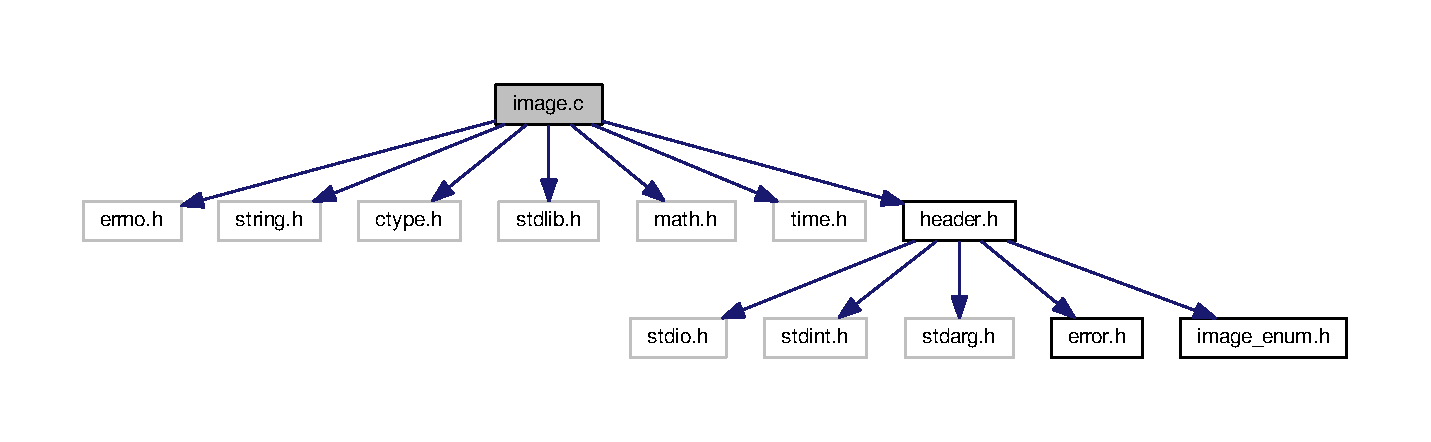
\includegraphics[width=350pt]{image_8c__incl}
\end{center}
\end{figure}
\subsection*{Functions}
\begin{DoxyCompactItemize}
\item 
\hyperlink{header_8h_ad8298d38a89742ed84029b278c6acee5}{Imel\+Image} $\ast$ \hyperlink{image_8c_af3a4abcb52f5611781065536fda0f97e}{imel\+\_\+image\+\_\+new} (\hyperlink{header_8h_af8a2b40c34eeed326846d0098ea84ec2}{Imel\+Size} width, \hyperlink{header_8h_af8a2b40c34eeed326846d0098ea84ec2}{Imel\+Size} height)
\begin{DoxyCompactList}\small\item\em Make a new image. \end{DoxyCompactList}\item 
\hyperlink{header_8h_ad8298d38a89742ed84029b278c6acee5}{Imel\+Image} $\ast$ \hyperlink{image_8c_a4692c85413196d5e15149cf4c66e1f08}{imel\+\_\+image\+\_\+new\+\_\+with\+\_\+background\+\_\+color} (\hyperlink{header_8h_af8a2b40c34eeed326846d0098ea84ec2}{Imel\+Size} width, \hyperlink{header_8h_af8a2b40c34eeed326846d0098ea84ec2}{Imel\+Size} height, \hyperlink{header_8h_add7dd9f8c093208bc4fd135a22a670ba}{Imel\+Pixel} pixel)
\begin{DoxyCompactList}\small\item\em Make a new image with background color and level specified. \end{DoxyCompactList}\item 
\hyperlink{header_8h_ad8298d38a89742ed84029b278c6acee5}{Imel\+Image} $\ast$ \hyperlink{image_8c_a8d41302f949cde87f3741455b3b9c23d}{imel\+\_\+image\+\_\+copy} (\hyperlink{header_8h_ad8298d38a89742ed84029b278c6acee5}{Imel\+Image} $\ast$image)
\begin{DoxyCompactList}\small\item\em Duplicate an image. \end{DoxyCompactList}\item 
\hyperlink{header_8h_af8a2b40c34eeed326846d0098ea84ec2}{Imel\+Size} \hyperlink{image_8c_a203143cba24be50f6d48eb50bcf64459}{imel\+\_\+image\+\_\+get\+\_\+width} (\hyperlink{header_8h_ad8298d38a89742ed84029b278c6acee5}{Imel\+Image} $\ast$image)
\begin{DoxyCompactList}\small\item\em Get image width. \end{DoxyCompactList}\item 
\hyperlink{header_8h_af8a2b40c34eeed326846d0098ea84ec2}{Imel\+Size} \hyperlink{image_8c_acb0158f7e2714802231d7beb651ec47d}{imel\+\_\+image\+\_\+get\+\_\+height} (\hyperlink{header_8h_ad8298d38a89742ed84029b278c6acee5}{Imel\+Image} $\ast$image)
\begin{DoxyCompactList}\small\item\em Get image height. \end{DoxyCompactList}\item 
void \hyperlink{image_8c_a873cba98c6f4f28e1db2bdf5da3cbfdd}{imel\+\_\+image\+\_\+free} (\hyperlink{header_8h_ad8298d38a89742ed84029b278c6acee5}{Imel\+Image} $\ast$image)
\begin{DoxyCompactList}\small\item\em Free an image. \end{DoxyCompactList}\item 
void \hyperlink{image_8c_af617e35a65519b8c9c33b49fc8e59e89}{imel\+\_\+image\+\_\+apply\+\_\+effect} (\hyperlink{header_8h_ad8298d38a89742ed84029b278c6acee5}{Imel\+Image} $\ast$image, \hyperlink{header_8h_a4919a9d01ef8388db452c59507d67f2e}{Imel\+Effect} effect,...)
\begin{DoxyCompactList}\small\item\em Apply an effect to an image. \end{DoxyCompactList}\item 
void \hyperlink{image_8c_abdb78af6d874ae54552a6f3219c75127}{imel\+\_\+image\+\_\+apply\+\_\+filter} (\hyperlink{header_8h_ad8298d38a89742ed84029b278c6acee5}{Imel\+Image} $\ast$image, \hyperlink{header_8h_a9facf73fdf3eb7434d01cd1c07341a28}{Imel\+Mask} mask)
\begin{DoxyCompactList}\small\item\em Apply a filter to an image. \end{DoxyCompactList}\item 
void \hyperlink{image_8c_a9a31b005b5160c7f4cfc5917136ff7e3}{imel\+\_\+image\+\_\+apply\+\_\+color} (\hyperlink{header_8h_ad8298d38a89742ed84029b278c6acee5}{Imel\+Image} $\ast$image, \hyperlink{header_8h_add1326f75f0c1a7da9f14c2ed4f673e9}{Imel\+Color} red, \hyperlink{header_8h_add1326f75f0c1a7da9f14c2ed4f673e9}{Imel\+Color} green, \hyperlink{header_8h_add1326f75f0c1a7da9f14c2ed4f673e9}{Imel\+Color} blue, \hyperlink{header_8h_a669b28ed18156f1a4f13732e070d6cf2}{bool} mono)
\begin{DoxyCompactList}\small\item\em Apply a color to an image. \end{DoxyCompactList}\item 
void \hyperlink{image_8c_ae2c499f2810e903a36b2b766541a815e}{imel\+\_\+image\+\_\+remove\+\_\+base\+\_\+color} (\hyperlink{header_8h_ad8298d38a89742ed84029b278c6acee5}{Imel\+Image} $\ast$image, \hyperlink{header_8h_a9facf73fdf3eb7434d01cd1c07341a28}{Imel\+Mask} mask)
\begin{DoxyCompactList}\small\item\em Remove a color. \end{DoxyCompactList}\item 
void \hyperlink{image_8c_a6975db091678649620213c772eafe0e4}{imel\+\_\+image\+\_\+apply\+\_\+color\+\_\+from\+\_\+string} (\hyperlink{header_8h_ad8298d38a89742ed84029b278c6acee5}{Imel\+Image} $\ast$image, const char $\ast$string, \hyperlink{header_8h_a669b28ed18156f1a4f13732e070d6cf2}{bool} mono)
\begin{DoxyCompactList}\small\item\em Apply a color from a string to an image. \end{DoxyCompactList}\item 
void \hyperlink{image_8c_a155f45bccd5beef204d410a7d399bc00}{imel\+\_\+image\+\_\+replace\+\_\+color} (\hyperlink{header_8h_ad8298d38a89742ed84029b278c6acee5}{Imel\+Image} $\ast$image, \hyperlink{header_8h_add7dd9f8c093208bc4fd135a22a670ba}{Imel\+Pixel} src, \hyperlink{header_8h_add7dd9f8c093208bc4fd135a22a670ba}{Imel\+Pixel} dest, \hyperlink{header_8h_af8a2b40c34eeed326846d0098ea84ec2}{Imel\+Size} tollerance)
\begin{DoxyCompactList}\small\item\em Replace a color with an other one. \end{DoxyCompactList}\item 
void \hyperlink{image_8c_a59e0bc363c90fe9e002b1e93e66475e8}{imel\+\_\+image\+\_\+replace\+\_\+area\+\_\+color} (\hyperlink{header_8h_ad8298d38a89742ed84029b278c6acee5}{Imel\+Image} $\ast$image, \hyperlink{header_8h_add7dd9f8c093208bc4fd135a22a670ba}{Imel\+Pixel} src, \hyperlink{header_8h_add7dd9f8c093208bc4fd135a22a670ba}{Imel\+Pixel} dest, \hyperlink{header_8h_af8a2b40c34eeed326846d0098ea84ec2}{Imel\+Size} tollerance, \hyperlink{header_8h_af8a2b40c34eeed326846d0098ea84ec2}{Imel\+Size} \+\_\+x1, \hyperlink{header_8h_af8a2b40c34eeed326846d0098ea84ec2}{Imel\+Size} \+\_\+y1, \hyperlink{header_8h_af8a2b40c34eeed326846d0098ea84ec2}{Imel\+Size} \+\_\+x2, \hyperlink{header_8h_af8a2b40c34eeed326846d0098ea84ec2}{Imel\+Size} \+\_\+y2)
\begin{DoxyCompactList}\small\item\em Replace a color with an other one in a specified area. \end{DoxyCompactList}\item 
\hyperlink{header_8h_ad8298d38a89742ed84029b278c6acee5}{Imel\+Image} $\ast$ \hyperlink{image_8c_affee2b61640d48e8528d6bb173c9bf33}{imel\+\_\+image\+\_\+resize} (\hyperlink{header_8h_ad8298d38a89742ed84029b278c6acee5}{Imel\+Image} $\ast$image, \hyperlink{header_8h_af8a2b40c34eeed326846d0098ea84ec2}{Imel\+Size} width, \hyperlink{header_8h_af8a2b40c34eeed326846d0098ea84ec2}{Imel\+Size} height)
\begin{DoxyCompactList}\small\item\em Resize an image. \end{DoxyCompactList}\item 
\hyperlink{header_8h_ad8298d38a89742ed84029b278c6acee5}{Imel\+Image} $\ast$ \hyperlink{image_8c_a18663716510e90c30ddcb2973071c08e}{imel\+\_\+image\+\_\+rotate\+\_\+to\+\_\+left} (\hyperlink{header_8h_ad8298d38a89742ed84029b278c6acee5}{Imel\+Image} $\ast$image)
\begin{DoxyCompactList}\small\item\em Rotate an image to left. \end{DoxyCompactList}\item 
\hyperlink{header_8h_ad8298d38a89742ed84029b278c6acee5}{Imel\+Image} $\ast$ \hyperlink{image_8c_a16511380a7ef0ed01a068f05273f8c08}{imel\+\_\+image\+\_\+rotate\+\_\+to\+\_\+right} (\hyperlink{header_8h_ad8298d38a89742ed84029b278c6acee5}{Imel\+Image} $\ast$image)
\begin{DoxyCompactList}\small\item\em Rotate an image to right. \end{DoxyCompactList}\item 
\hyperlink{header_8h_ad8298d38a89742ed84029b278c6acee5}{Imel\+Image} $\ast$ \hyperlink{image_8c_a825a1b2309c771735d1c1379b484076d}{imel\+\_\+image\+\_\+rotate\+\_\+complete} (\hyperlink{header_8h_ad8298d38a89742ed84029b278c6acee5}{Imel\+Image} $\ast$image)
\begin{DoxyCompactList}\small\item\em Rotate an image to 180 degrees. \end{DoxyCompactList}\item 
\hyperlink{header_8h_ad8298d38a89742ed84029b278c6acee5}{Imel\+Image} $\ast$ \hyperlink{image_8c_a4a2cd319143d8bcc9cd60cc191713664}{imel\+\_\+image\+\_\+mirror\+\_\+horizontal} (\hyperlink{header_8h_ad8298d38a89742ed84029b278c6acee5}{Imel\+Image} $\ast$image)
\begin{DoxyCompactList}\small\item\em Mirror an image to horizontal. \end{DoxyCompactList}\item 
\hyperlink{header_8h_ad8298d38a89742ed84029b278c6acee5}{Imel\+Image} $\ast$ \hyperlink{image_8c_a9e7cf1420d1937b0528104da21bab4c2}{imel\+\_\+image\+\_\+mirror\+\_\+vertical} (\hyperlink{header_8h_ad8298d38a89742ed84029b278c6acee5}{Imel\+Image} $\ast$image)
\begin{DoxyCompactList}\small\item\em Mirror an image to vertical. \end{DoxyCompactList}\item 
\hyperlink{header_8h_ad8298d38a89742ed84029b278c6acee5}{Imel\+Image} $\ast$ \hyperlink{image_8c_adac45043cb30a449868c1a7526671504}{imel\+\_\+image\+\_\+rotate} (\hyperlink{header_8h_ad8298d38a89742ed84029b278c6acee5}{Imel\+Image} $\ast$image, double rotate\+\_\+rad)
\begin{DoxyCompactList}\small\item\em Rotate an image to a chosen angle. \end{DoxyCompactList}\item 
\hyperlink{header_8h_ad8298d38a89742ed84029b278c6acee5}{Imel\+Image} $\ast$ \hyperlink{image_8c_ad08c629d2c44d24e7c485b7ff9a28021}{imel\+\_\+image\+\_\+perspective} (\hyperlink{header_8h_ad8298d38a89742ed84029b278c6acee5}{Imel\+Image} $\ast$image, double rad\+\_\+angle, \hyperlink{header_8h_aef27fcac7a96d118b3c3194c2577049f}{Imel\+Orientation} orientation)
\begin{DoxyCompactList}\small\item\em Makes an horizontal or vertical perspective. \end{DoxyCompactList}\item 
\hyperlink{header_8h_ad8298d38a89742ed84029b278c6acee5}{Imel\+Image} $\ast$ \hyperlink{image_8c_a54960c7fec6873dc13d2069d3c9eb718}{imel\+\_\+image\+\_\+cut} (\hyperlink{header_8h_ad8298d38a89742ed84029b278c6acee5}{Imel\+Image} $\ast$image, \hyperlink{header_8h_af8a2b40c34eeed326846d0098ea84ec2}{Imel\+Size} sx, \hyperlink{header_8h_af8a2b40c34eeed326846d0098ea84ec2}{Imel\+Size} sy, \hyperlink{header_8h_af8a2b40c34eeed326846d0098ea84ec2}{Imel\+Size} ex, \hyperlink{header_8h_af8a2b40c34eeed326846d0098ea84ec2}{Imel\+Size} ey)
\begin{DoxyCompactList}\small\item\em Cut an image. \end{DoxyCompactList}\item 
\hyperlink{header_8h_ad8298d38a89742ed84029b278c6acee5}{Imel\+Image} $\ast$$\ast$ \hyperlink{image_8c_a31943792f957de747e49b6dc1fbbab05}{imel\+\_\+image\+\_\+cut\+\_\+grid} (\hyperlink{header_8h_ad8298d38a89742ed84029b278c6acee5}{Imel\+Image} $\ast$image, \hyperlink{header_8h_a3f4de920943cb4d0979d415b4c5e3989}{Imel\+Info\+Cut} $\ast$cut\+\_\+info)
\begin{DoxyCompactList}\small\item\em Cut an image in more images. \end{DoxyCompactList}\item 
\hyperlink{header_8h_ad8298d38a89742ed84029b278c6acee5}{Imel\+Image} $\ast$ \hyperlink{image_8c_a75fbdaa484f8b191b8988af68181c488}{imel\+\_\+image\+\_\+auto\+\_\+cut} (\hyperlink{header_8h_ad8298d38a89742ed84029b278c6acee5}{Imel\+Image} $\ast$image, \hyperlink{header_8h_af8a2b40c34eeed326846d0098ea84ec2}{Imel\+Size} tollerance, \hyperlink{header_8h_a6182c8947d12d828155f0fb8cb024209}{Imel\+Ref} reference,...)
\begin{DoxyCompactList}\small\item\em Cut automatically an image. \end{DoxyCompactList}\item 
void \hyperlink{image_8c_acdefba6da2457b909d9ca2600a13bc65}{imel\+\_\+image\+\_\+insert\+\_\+image} (\hyperlink{header_8h_ad8298d38a89742ed84029b278c6acee5}{Imel\+Image} $\ast$dest, \hyperlink{header_8h_ad8298d38a89742ed84029b278c6acee5}{Imel\+Image} $\ast$src, \hyperlink{header_8h_af8a2b40c34eeed326846d0098ea84ec2}{Imel\+Size} sx, \hyperlink{header_8h_af8a2b40c34eeed326846d0098ea84ec2}{Imel\+Size} sy)
\begin{DoxyCompactList}\small\item\em Insert an image in another one. \end{DoxyCompactList}\item 
\hyperlink{header_8h_ad8298d38a89742ed84029b278c6acee5}{Imel\+Image} $\ast$ \hyperlink{image_8c_acbb25e82ef469246170ce9b541a4d220}{imel\+\_\+image\+\_\+apply\+\_\+logic\+\_\+operation} (\hyperlink{header_8h_ad8298d38a89742ed84029b278c6acee5}{Imel\+Image} $\ast$img1, \hyperlink{header_8h_ad8298d38a89742ed84029b278c6acee5}{Imel\+Image} $\ast$img2, \hyperlink{header_8h_af92bba14d49d8e59b2642eb300fedb5e}{Imel\+Logic\+Operation} logic\+\_\+operation)
\begin{DoxyCompactList}\small\item\em Apply a logic operation between two images. \end{DoxyCompactList}\item 
int $\ast$ \hyperlink{image_8c_afa2cd389929358c87f2d21e1e7b2ef9a}{imel\+\_\+image\+\_\+get\+\_\+histogram} (\hyperlink{header_8h_ad8298d38a89742ed84029b278c6acee5}{Imel\+Image} $\ast$image, \hyperlink{header_8h_a8879c5e403ddb26c326b1cc2c3e529bf}{Imel\+Histogram} histogram\+\_\+type)
\begin{DoxyCompactList}\small\item\em Get histogram values from an image. \end{DoxyCompactList}\item 
\hyperlink{header_8h_ad8298d38a89742ed84029b278c6acee5}{Imel\+Image} $\ast$ \hyperlink{image_8c_ae416e85c63ce2f3f60df3fb31c5d41b5}{imel\+\_\+image\+\_\+get\+\_\+histogram\+\_\+image} (\hyperlink{header_8h_ad8298d38a89742ed84029b278c6acee5}{Imel\+Image} $\ast$image, int $\ast$\+\_\+\+\_\+histogram, \hyperlink{header_8h_a8879c5e403ddb26c326b1cc2c3e529bf}{Imel\+Histogram} histogram\+\_\+type)
\begin{DoxyCompactList}\small\item\em Make an histogram image for an image chosen. \end{DoxyCompactList}\item 
\hyperlink{header_8h_ad8298d38a89742ed84029b278c6acee5}{Imel\+Image} $\ast$ \hyperlink{image_8c_a41cc4f146e4863e1969bfa15ca3e7afc}{imel\+\_\+image\+\_\+get\+\_\+histograms\+\_\+image} (\hyperlink{header_8h_ad8298d38a89742ed84029b278c6acee5}{Imel\+Image} $\ast$image, \hyperlink{header_8h_aacf376be43512b219081df71ed7ee438}{Imel\+Histogram\+Layout} layout)
\begin{DoxyCompactList}\small\item\em Make all types of histogram of an image. \end{DoxyCompactList}\item 
void \hyperlink{image_8c_a5fd7c413bcd1025d2c94810d66ba36eb}{imel\+\_\+image\+\_\+change\+\_\+level} (\hyperlink{header_8h_ad8298d38a89742ed84029b278c6acee5}{Imel\+Image} $\ast$image, \hyperlink{header_8h_abece8958e8db1e2826f21fd822c14694}{Imel\+Level\+Operation} level\+\_\+operation, \hyperlink{header_8h_a97bc4b146a807c2d83b966983132f4fc}{Imel\+Level} level)
\begin{DoxyCompactList}\small\item\em Change level of an image. \end{DoxyCompactList}\item 
void \hyperlink{image_8c_a3e8526c34b3cb916894f09923ea2a116}{imel\+\_\+image\+\_\+change\+\_\+color\+\_\+level} (\hyperlink{header_8h_ad8298d38a89742ed84029b278c6acee5}{Imel\+Image} $\ast$image, \hyperlink{header_8h_abece8958e8db1e2826f21fd822c14694}{Imel\+Level\+Operation} level\+\_\+operation, \hyperlink{header_8h_a97bc4b146a807c2d83b966983132f4fc}{Imel\+Level} level, \hyperlink{header_8h_add7dd9f8c093208bc4fd135a22a670ba}{Imel\+Pixel} color\+\_\+pxl, \hyperlink{header_8h_add1326f75f0c1a7da9f14c2ed4f673e9}{Imel\+Color} tollerance)
\begin{DoxyCompactList}\small\item\em Change level to a specified color. \end{DoxyCompactList}\item 
void \hyperlink{image_8c_a52a572198c8e082a7efeb5acc5dfab8e}{imel\+\_\+image\+\_\+apply\+\_\+convolution} (\hyperlink{header_8h_ad8298d38a89742ed84029b278c6acee5}{Imel\+Image} $\ast$image, double $\ast$$\ast$filter, int width, int height, double factor, double bias)
\begin{DoxyCompactList}\small\item\em Apply a convolution matrix to an image. \end{DoxyCompactList}\item 
void \hyperlink{image_8c_af026795ee048b2294876418c64729d03}{imel\+\_\+image\+\_\+apply\+\_\+pattern} (\hyperlink{header_8h_ad8298d38a89742ed84029b278c6acee5}{Imel\+Image} $\ast$image, \hyperlink{header_8h_ad8298d38a89742ed84029b278c6acee5}{Imel\+Image} $\ast$pattern, \hyperlink{header_8h_a7321d084db08c3a51089e8a4612b332b}{Imel\+Pattern\+Operation} operation)
\begin{DoxyCompactList}\small\item\em Apply a pattern to an imaage. \end{DoxyCompactList}\item 
\hyperlink{header_8h_ad8298d38a89742ed84029b278c6acee5}{Imel\+Image} $\ast$ \hyperlink{image_8c_a12519cad063897a1dcf9eb4c677b8304}{imel\+\_\+image\+\_\+union} (\hyperlink{header_8h_ad8298d38a89742ed84029b278c6acee5}{Imel\+Image} $\ast$img1, \hyperlink{header_8h_ad8298d38a89742ed84029b278c6acee5}{Imel\+Image} $\ast$img2, unsigned char opacity, \hyperlink{header_8h_a4d620b3c547205ca76d92f43f09320d1}{Imel\+Alignment} alignment)
\begin{DoxyCompactList}\small\item\em Insert an image in another with a chosen opacity. \end{DoxyCompactList}\item 
\hyperlink{header_8h_ad8298d38a89742ed84029b278c6acee5}{Imel\+Image} $\ast$ \hyperlink{image_8c_aa517733f37a96bfcccf4ee666a92b206}{imel\+\_\+image\+\_\+slant} (\hyperlink{header_8h_ad8298d38a89742ed84029b278c6acee5}{Imel\+Image} $\ast$image, \hyperlink{header_8h_af8a2b40c34eeed326846d0098ea84ec2}{Imel\+Size} x0, \hyperlink{header_8h_af8a2b40c34eeed326846d0098ea84ec2}{Imel\+Size} y0, \hyperlink{header_8h_af8a2b40c34eeed326846d0098ea84ec2}{Imel\+Size} x1, \hyperlink{header_8h_af8a2b40c34eeed326846d0098ea84ec2}{Imel\+Size} y1, \hyperlink{header_8h_aef27fcac7a96d118b3c3194c2577049f}{Imel\+Orientation} orientation, \hyperlink{header_8h_a669b28ed18156f1a4f13732e070d6cf2}{bool} lengthens)
\begin{DoxyCompactList}\small\item\em Slant an image or a small area inside it. \end{DoxyCompactList}\item 
void \hyperlink{image_8c_a66997f20203b384d1185a1dd9985dd67}{imel\+\_\+image\+\_\+shift} (\hyperlink{header_8h_ad8298d38a89742ed84029b278c6acee5}{Imel\+Image} $\ast$image, \hyperlink{header_8h_aef27fcac7a96d118b3c3194c2577049f}{Imel\+Orientation} orientation, long int move\+\_\+pxl, \hyperlink{header_8h_a669b28ed18156f1a4f13732e070d6cf2}{bool} lengthens)
\begin{DoxyCompactList}\small\item\em Shift an image. \end{DoxyCompactList}\item 
\hyperlink{header_8h_a669b28ed18156f1a4f13732e070d6cf2}{bool} \hyperlink{image_8c_add471c449ecce1b4bd78fc34a698f44f}{imel\+\_\+image\+\_\+shift\+\_\+lines} (\hyperlink{header_8h_ad8298d38a89742ed84029b278c6acee5}{Imel\+Image} $\ast$image, \hyperlink{header_8h_aef27fcac7a96d118b3c3194c2577049f}{Imel\+Orientation} move\+\_\+type, \hyperlink{header_8h_af8a2b40c34eeed326846d0098ea84ec2}{Imel\+Size} line, \hyperlink{header_8h_af8a2b40c34eeed326846d0098ea84ec2}{Imel\+Size} width, long int move\+\_\+pixel, \hyperlink{header_8h_a669b28ed18156f1a4f13732e070d6cf2}{bool} lengthens)
\begin{DoxyCompactList}\small\item\em Shift only some image lines. \end{DoxyCompactList}\item 
void \hyperlink{image_8c_a3b9a4fb2f3fd678b206196e9f9bf4889}{imel\+\_\+image\+\_\+shift\+\_\+bpc} (\hyperlink{header_8h_ad8298d38a89742ed84029b278c6acee5}{Imel\+Image} $\ast$image, int bpc\+\_\+shift\+\_\+red, int bpc\+\_\+shift\+\_\+green, int bpc\+\_\+shift\+\_\+blue)
\begin{DoxyCompactList}\small\item\em Shift the R\+GB values of an image. \end{DoxyCompactList}\item 
void \hyperlink{image_8c_aedeae21c9710c31bf78b5a12d03a031f}{imel\+\_\+image\+\_\+remove\+\_\+noise} (\hyperlink{header_8h_ad8298d38a89742ed84029b278c6acee5}{Imel\+Image} $\ast$image, \hyperlink{header_8h_af8a2b40c34eeed326846d0098ea84ec2}{Imel\+Size} size\+\_\+q, \hyperlink{header_8h_a9facf73fdf3eb7434d01cd1c07341a28}{Imel\+Mask} mask, \hyperlink{header_8h_add1326f75f0c1a7da9f14c2ed4f673e9}{Imel\+Color} tollerance)
\begin{DoxyCompactList}\small\item\em Remove noise from an image. \end{DoxyCompactList}\item 
void \hyperlink{image_8c_a5b3d70708a116076bfbcaeb7a9cd2b5d}{imel\+\_\+image\+\_\+apply\+\_\+noise} (\hyperlink{header_8h_ad8298d38a89742ed84029b278c6acee5}{Imel\+Image} $\ast$image, \hyperlink{header_8h_add1326f75f0c1a7da9f14c2ed4f673e9}{Imel\+Color} noise\+\_\+range, \hyperlink{header_8h_af8a2b40c34eeed326846d0098ea84ec2}{Imel\+Size} noise\+\_\+quantity, \hyperlink{header_8h_a9facf73fdf3eb7434d01cd1c07341a28}{Imel\+Mask} mask, \hyperlink{header_8h_abb411905768327b93668c636957a73ff}{Imel\+Noise\+Operation} operation, \hyperlink{header_8h_a669b28ed18156f1a4f13732e070d6cf2}{bool} nepc)
\begin{DoxyCompactList}\small\item\em Apply a noise to an image. \end{DoxyCompactList}\end{DoxyCompactItemize}


\subsection{Detailed Description}
This file contains functions to elaborate images. 

\begin{DoxyAuthor}{Author}
Davide Francesco Merico 
\end{DoxyAuthor}


\subsection{Function Documentation}
\index{image.\+c@{image.\+c}!imel\+\_\+image\+\_\+apply\+\_\+color@{imel\+\_\+image\+\_\+apply\+\_\+color}}
\index{imel\+\_\+image\+\_\+apply\+\_\+color@{imel\+\_\+image\+\_\+apply\+\_\+color}!image.\+c@{image.\+c}}
\subsubsection[{\texorpdfstring{imel\+\_\+image\+\_\+apply\+\_\+color(\+Imel\+Image $\ast$image, Imel\+Color red, Imel\+Color green, Imel\+Color blue, bool mono)}{imel_image_apply_color(ImelImage *image, ImelColor red, ImelColor green, ImelColor blue, bool mono)}}]{\setlength{\rightskip}{0pt plus 5cm}void imel\+\_\+image\+\_\+apply\+\_\+color (
\begin{DoxyParamCaption}
\item[{{\bf Imel\+Image} $\ast$}]{image, }
\item[{{\bf Imel\+Color}}]{red, }
\item[{{\bf Imel\+Color}}]{green, }
\item[{{\bf Imel\+Color}}]{blue, }
\item[{{\bf bool}}]{mono}
\end{DoxyParamCaption}
)}\hypertarget{image_8c_a9a31b005b5160c7f4cfc5917136ff7e3}{}\label{image_8c_a9a31b005b5160c7f4cfc5917136ff7e3}


Apply a color to an image. 

This function apply a chosen color to the {\ttfamily image}. It can be set as unique color or as reference to existed color in {\ttfamily image}.


\begin{DoxyCode}
1 ImelImage *image = imel\_image\_new\_from ("image.jpg", 0, NULL);
2 
3 imel\_image\_apply\_color (image, 0xfd, 0xb4, 0x55, false);
4 ...
5 imel\_image\_apply\_color (image, 0xfd, 0xb4, ox55, true);
\end{DoxyCode}
 
\begin{DoxyImage}
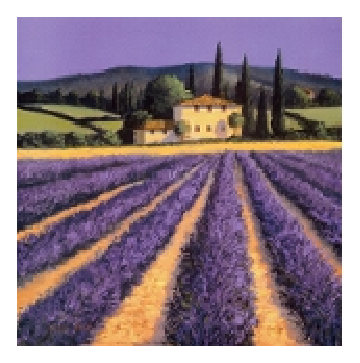
\includegraphics[width=\textwidth,height=\textheight/2,keepaspectratio=true]{images/orig}
\caption{Original Image}
\end{DoxyImage}

\begin{DoxyImage}
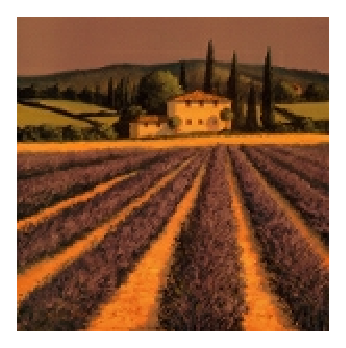
\includegraphics[width=\textwidth,height=\textheight/2,keepaspectratio=true]{images/imac-f}
\caption{Passed F\+A\+L\+SE as last argument}
\end{DoxyImage}

\begin{DoxyImage}
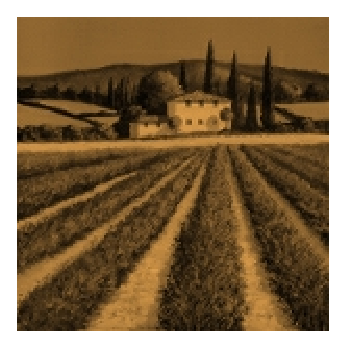
\includegraphics[width=\textwidth,height=\textheight/2,keepaspectratio=true]{images/imac-t}
\caption{Passed T\+R\+UE as last argument}
\end{DoxyImage}

\begin{DoxyParams}{Parameters}
{\em image} & Image on which apply the color \\
\hline
{\em red} & Red channel of the color to apply \\
\hline
{\em green} & Green channel of the color to apply \\
\hline
{\em blue} & Blue channel of the color to apply \\
\hline
{\em mono} & T\+R\+UE if the color chosen is the only color of the image, else F\+A\+L\+SE \\
\hline
\end{DoxyParams}
\begin{DoxySeeAlso}{See also}
\hyperlink{image_8c_a6975db091678649620213c772eafe0e4}{imel\+\_\+image\+\_\+apply\+\_\+color\+\_\+from\+\_\+string} 
\end{DoxySeeAlso}
\index{image.\+c@{image.\+c}!imel\+\_\+image\+\_\+apply\+\_\+color\+\_\+from\+\_\+string@{imel\+\_\+image\+\_\+apply\+\_\+color\+\_\+from\+\_\+string}}
\index{imel\+\_\+image\+\_\+apply\+\_\+color\+\_\+from\+\_\+string@{imel\+\_\+image\+\_\+apply\+\_\+color\+\_\+from\+\_\+string}!image.\+c@{image.\+c}}
\subsubsection[{\texorpdfstring{imel\+\_\+image\+\_\+apply\+\_\+color\+\_\+from\+\_\+string(\+Imel\+Image $\ast$image, const char $\ast$string, bool mono)}{imel_image_apply_color_from_string(ImelImage *image, const char *string, bool mono)}}]{\setlength{\rightskip}{0pt plus 5cm}void imel\+\_\+image\+\_\+apply\+\_\+color\+\_\+from\+\_\+string (
\begin{DoxyParamCaption}
\item[{{\bf Imel\+Image} $\ast$}]{image, }
\item[{const char $\ast$}]{string, }
\item[{{\bf bool}}]{mono}
\end{DoxyParamCaption}
)}\hypertarget{image_8c_a6975db091678649620213c772eafe0e4}{}\label{image_8c_a6975db091678649620213c772eafe0e4}


Apply a color from a string to an image. 

This function apply a chosen color from a string to the {\ttfamily image}. It can be set as unique color or as reference to existed color in {\ttfamily image}.


\begin{DoxyParams}{Parameters}
{\em image} & Image on which apply the color \\
\hline
{\em string} & Color to apply to the image in H\+T\+ML format ( \textquotesingle{}\#rrggbb\textquotesingle{} ) \\
\hline
{\em mono} & T\+R\+UE if the color chosen is the only color of the image, else F\+A\+L\+SE \\
\hline
\end{DoxyParams}
\begin{DoxySeeAlso}{See also}
\hyperlink{image_8c_a9a31b005b5160c7f4cfc5917136ff7e3}{imel\+\_\+image\+\_\+apply\+\_\+color} 
\end{DoxySeeAlso}
\index{image.\+c@{image.\+c}!imel\+\_\+image\+\_\+apply\+\_\+convolution@{imel\+\_\+image\+\_\+apply\+\_\+convolution}}
\index{imel\+\_\+image\+\_\+apply\+\_\+convolution@{imel\+\_\+image\+\_\+apply\+\_\+convolution}!image.\+c@{image.\+c}}
\subsubsection[{\texorpdfstring{imel\+\_\+image\+\_\+apply\+\_\+convolution(\+Imel\+Image $\ast$image, double $\ast$$\ast$filter, int width, int height, double factor, double bias)}{imel_image_apply_convolution(ImelImage *image, double **filter, int width, int height, double factor, double bias)}}]{\setlength{\rightskip}{0pt plus 5cm}void imel\+\_\+image\+\_\+apply\+\_\+convolution (
\begin{DoxyParamCaption}
\item[{{\bf Imel\+Image} $\ast$}]{image, }
\item[{double $\ast$$\ast$}]{filter, }
\item[{int}]{width, }
\item[{int}]{height, }
\item[{double}]{factor, }
\item[{double}]{bias}
\end{DoxyParamCaption}
)}\hypertarget{image_8c_a52a572198c8e082a7efeb5acc5dfab8e}{}\label{image_8c_a52a572198c8e082a7efeb5acc5dfab8e}


Apply a convolution matrix to an image. 

This function apply a convolution matrix of chosen size to {\ttfamily image}.


\begin{DoxyParams}{Parameters}
{\em image} & Image to apply the {\ttfamily filter} \\
\hline
{\em filter} & Convolution matrix \\
\hline
{\em width} & Width of matrix \\
\hline
{\em height} & Height of matrix \\
\hline
{\em factor} & Multiply factor \\
\hline
{\em bias} & Offset to apply to matrix\\
\hline
\end{DoxyParams}
\begin{DoxySeeAlso}{See also}
\href{https://en.wikipedia.org/wiki/Kernel_(image_processing)}{\tt https\+://en.\+wikipedia.\+org/wiki/\+Kernel\+\_\+(image\+\_\+processing)} 
\end{DoxySeeAlso}
\index{image.\+c@{image.\+c}!imel\+\_\+image\+\_\+apply\+\_\+effect@{imel\+\_\+image\+\_\+apply\+\_\+effect}}
\index{imel\+\_\+image\+\_\+apply\+\_\+effect@{imel\+\_\+image\+\_\+apply\+\_\+effect}!image.\+c@{image.\+c}}
\subsubsection[{\texorpdfstring{imel\+\_\+image\+\_\+apply\+\_\+effect(\+Imel\+Image $\ast$image, Imel\+Effect effect,...)}{imel_image_apply_effect(ImelImage *image, ImelEffect effect,...)}}]{\setlength{\rightskip}{0pt plus 5cm}void imel\+\_\+image\+\_\+apply\+\_\+effect (
\begin{DoxyParamCaption}
\item[{{\bf Imel\+Image} $\ast$}]{image, }
\item[{{\bf Imel\+Effect}}]{effect, }
\item[{}]{...}
\end{DoxyParamCaption}
)}\hypertarget{image_8c_af617e35a65519b8c9c33b49fc8e59e89}{}\label{image_8c_af617e35a65519b8c9c33b49fc8e59e89}


Apply an effect to an image. 

This function apply the {\ttfamily effect} to the {\ttfamily image}.


\begin{DoxyParams}{Parameters}
{\em image} & Image on which apply the {\ttfamily effect} \\
\hline
{\em effect} & Effect to apply to the {\ttfamily image} \\
\hline
{\em ...} & Options for the {\ttfamily effect} \\
\hline
\end{DoxyParams}
\begin{DoxySeeAlso}{See also}
\hyperlink{header_8h_a4919a9d01ef8388db452c59507d67f2e}{Imel\+Effect} 
\end{DoxySeeAlso}
\index{image.\+c@{image.\+c}!imel\+\_\+image\+\_\+apply\+\_\+filter@{imel\+\_\+image\+\_\+apply\+\_\+filter}}
\index{imel\+\_\+image\+\_\+apply\+\_\+filter@{imel\+\_\+image\+\_\+apply\+\_\+filter}!image.\+c@{image.\+c}}
\subsubsection[{\texorpdfstring{imel\+\_\+image\+\_\+apply\+\_\+filter(\+Imel\+Image $\ast$image, Imel\+Mask mask)}{imel_image_apply_filter(ImelImage *image, ImelMask mask)}}]{\setlength{\rightskip}{0pt plus 5cm}void imel\+\_\+image\+\_\+apply\+\_\+filter (
\begin{DoxyParamCaption}
\item[{{\bf Imel\+Image} $\ast$}]{image, }
\item[{{\bf Imel\+Mask}}]{mask}
\end{DoxyParamCaption}
)}\hypertarget{image_8c_abdb78af6d874ae54552a6f3219c75127}{}\label{image_8c_abdb78af6d874ae54552a6f3219c75127}


Apply a filter to an image. 

This function set to 255 the channel, or the channels, specified as {\ttfamily mask}.


\begin{DoxyCode}
1 ImelImage *image = imel\_image\_new\_from ("image.jpg", 0, NULL);
2 
3 imel\_image\_apply\_filter (image, IMEL\_MASK\_RED | IMEL\_MASK\_BLUE);
\end{DoxyCode}



\begin{DoxyParams}{Parameters}
{\em image} & Image on which apply the filter \\
\hline
{\em mask} & Channel, or channels, to set to 255. \\
\hline
\end{DoxyParams}
\begin{DoxySeeAlso}{See also}
\hyperlink{header_8h_a9facf73fdf3eb7434d01cd1c07341a28}{Imel\+Mask} 

\hyperlink{image_8c_ae2c499f2810e903a36b2b766541a815e}{imel\+\_\+image\+\_\+remove\+\_\+base\+\_\+color} 
\end{DoxySeeAlso}
\index{image.\+c@{image.\+c}!imel\+\_\+image\+\_\+apply\+\_\+logic\+\_\+operation@{imel\+\_\+image\+\_\+apply\+\_\+logic\+\_\+operation}}
\index{imel\+\_\+image\+\_\+apply\+\_\+logic\+\_\+operation@{imel\+\_\+image\+\_\+apply\+\_\+logic\+\_\+operation}!image.\+c@{image.\+c}}
\subsubsection[{\texorpdfstring{imel\+\_\+image\+\_\+apply\+\_\+logic\+\_\+operation(\+Imel\+Image $\ast$img1, Imel\+Image $\ast$img2, Imel\+Logic\+Operation logic\+\_\+operation)}{imel_image_apply_logic_operation(ImelImage *img1, ImelImage *img2, ImelLogicOperation logic_operation)}}]{\setlength{\rightskip}{0pt plus 5cm}{\bf Imel\+Image}$\ast$ imel\+\_\+image\+\_\+apply\+\_\+logic\+\_\+operation (
\begin{DoxyParamCaption}
\item[{{\bf Imel\+Image} $\ast$}]{img1, }
\item[{{\bf Imel\+Image} $\ast$}]{img2, }
\item[{{\bf Imel\+Logic\+Operation}}]{logic\+\_\+operation}
\end{DoxyParamCaption}
)}\hypertarget{image_8c_acbb25e82ef469246170ce9b541a4d220}{}\label{image_8c_acbb25e82ef469246170ce9b541a4d220}


Apply a logic operation between two images. 

This function apply the {\ttfamily logic\+\_\+operation} to {\ttfamily img1} and {\ttfamily img2}.


\begin{DoxyParams}{Parameters}
{\em img1} & First image \\
\hline
{\em img2} & Second image \\
\hline
{\em logic\+\_\+operation} & Type of operation \\
\hline
\end{DoxyParams}
\begin{DoxyReturn}{Returns}
An image result from the operation between {\ttfamily img1} and {\ttfamily img2} 
\end{DoxyReturn}
\begin{DoxySeeAlso}{See also}
\hyperlink{header_8h_af92bba14d49d8e59b2642eb300fedb5e}{Imel\+Logic\+Operation} 
\end{DoxySeeAlso}
\index{image.\+c@{image.\+c}!imel\+\_\+image\+\_\+apply\+\_\+noise@{imel\+\_\+image\+\_\+apply\+\_\+noise}}
\index{imel\+\_\+image\+\_\+apply\+\_\+noise@{imel\+\_\+image\+\_\+apply\+\_\+noise}!image.\+c@{image.\+c}}
\subsubsection[{\texorpdfstring{imel\+\_\+image\+\_\+apply\+\_\+noise(\+Imel\+Image $\ast$image, Imel\+Color noise\+\_\+range, Imel\+Size noise\+\_\+quantity, Imel\+Mask mask, Imel\+Noise\+Operation operation, bool nepc)}{imel_image_apply_noise(ImelImage *image, ImelColor noise_range, ImelSize noise_quantity, ImelMask mask, ImelNoiseOperation operation, bool nepc)}}]{\setlength{\rightskip}{0pt plus 5cm}void imel\+\_\+image\+\_\+apply\+\_\+noise (
\begin{DoxyParamCaption}
\item[{{\bf Imel\+Image} $\ast$}]{image, }
\item[{{\bf Imel\+Color}}]{noise\+\_\+range, }
\item[{{\bf Imel\+Size}}]{noise\+\_\+quantity, }
\item[{{\bf Imel\+Mask}}]{mask, }
\item[{{\bf Imel\+Noise\+Operation}}]{operation, }
\item[{{\bf bool}}]{nepc}
\end{DoxyParamCaption}
)}\hypertarget{image_8c_a5b3d70708a116076bfbcaeb7a9cd2b5d}{}\label{image_8c_a5b3d70708a116076bfbcaeb7a9cd2b5d}


Apply a noise to an image. 

This function apply a noise to {\ttfamily image} at one or more R\+GB channels.


\begin{DoxyCode}
1 ImelImage *image = imel\_image\_new\_from ("apply\_noise.jpg", 0, NULL);
2 ImelMask mask = IMEL\_MASK\_RED | IMEL\_MASK\_GREEN | IMEL\_MASK\_BLUE;
3 
4 imel\_image\_apply\_noise (image, 90, 30, mask, IMEL\_NOISE\_OPERATION\_SUM, false);
\end{DoxyCode}
 
\begin{DoxyImage}
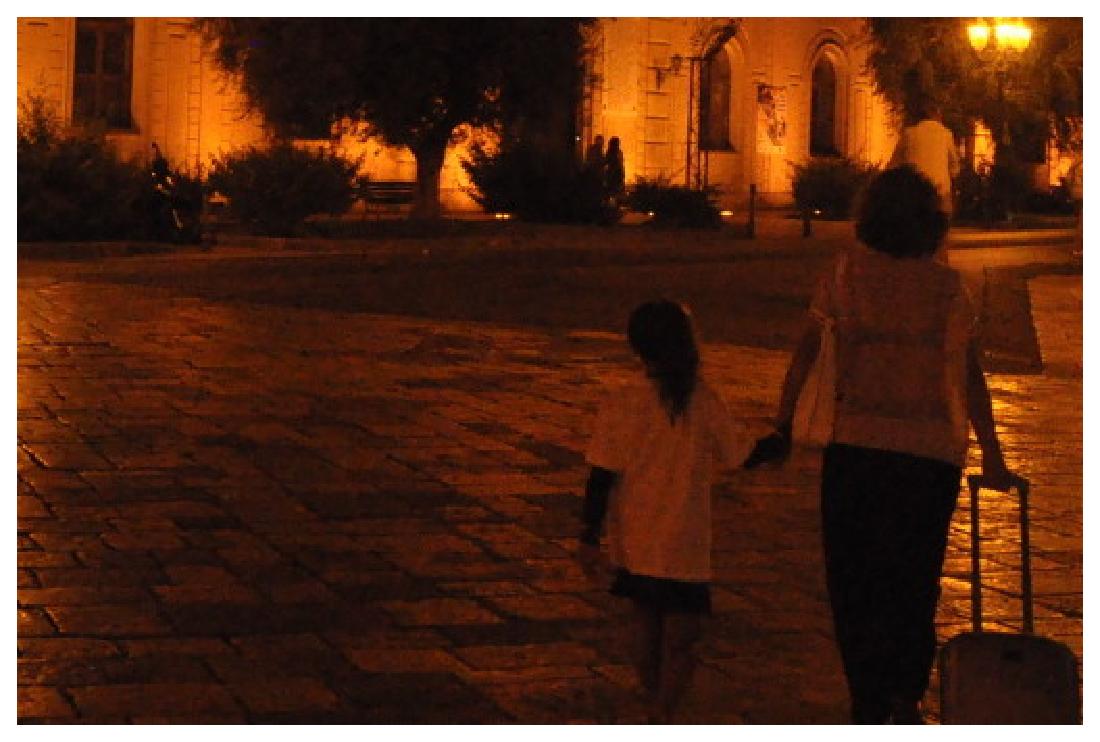
\includegraphics[width=\textwidth,height=\textheight/2,keepaspectratio=true]{images/noise}
\caption{Input Image}
\end{DoxyImage}

\begin{DoxyImage}
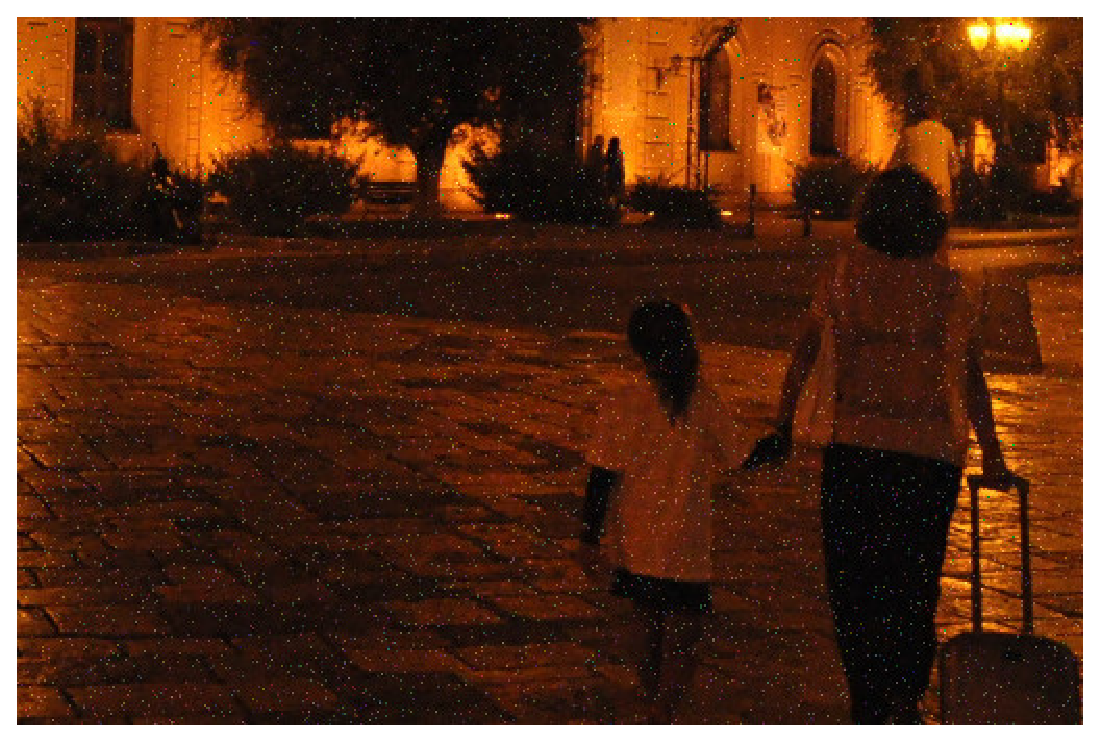
\includegraphics[width=\textwidth,height=\textheight/2,keepaspectratio=true]{images/apply_noise}
\caption{Result Image}
\end{DoxyImage}
 
\begin{DoxyParams}{Parameters}
{\em image} & Image to apply the noise \\
\hline
{\em noise\+\_\+range} & Value for {\ttfamily operation}. This value specifies the max value can be added, subtracted, multiply or divided when noise is applied. \\
\hline
{\em noise\+\_\+quantity} & Specifies how much noise can be applied randomly to image. Values\+: 1 for apply the noise to each pixel, 4294967295 is the max value. \\
\hline
{\em mask} & Channels affected from noise. \\
\hline
{\em operation} & Operation to do when apply the noise \\
\hline
{\em nepc} & If T\+R\+UE apply the noise value calculated to each R\+GB channel specified, else each noise value will be calculated separately.\\
\hline
\end{DoxyParams}
\begin{DoxySeeAlso}{See also}
\hyperlink{header_8h_abb411905768327b93668c636957a73ff}{Imel\+Noise\+Operation} 

\hyperlink{image_8c_aedeae21c9710c31bf78b5a12d03a031f}{imel\+\_\+image\+\_\+remove\+\_\+noise} 
\end{DoxySeeAlso}
\index{image.\+c@{image.\+c}!imel\+\_\+image\+\_\+apply\+\_\+pattern@{imel\+\_\+image\+\_\+apply\+\_\+pattern}}
\index{imel\+\_\+image\+\_\+apply\+\_\+pattern@{imel\+\_\+image\+\_\+apply\+\_\+pattern}!image.\+c@{image.\+c}}
\subsubsection[{\texorpdfstring{imel\+\_\+image\+\_\+apply\+\_\+pattern(\+Imel\+Image $\ast$image, Imel\+Image $\ast$pattern, Imel\+Pattern\+Operation operation)}{imel_image_apply_pattern(ImelImage *image, ImelImage *pattern, ImelPatternOperation operation)}}]{\setlength{\rightskip}{0pt plus 5cm}void imel\+\_\+image\+\_\+apply\+\_\+pattern (
\begin{DoxyParamCaption}
\item[{{\bf Imel\+Image} $\ast$}]{image, }
\item[{{\bf Imel\+Image} $\ast$}]{pattern, }
\item[{{\bf Imel\+Pattern\+Operation}}]{operation}
\end{DoxyParamCaption}
)}\hypertarget{image_8c_af026795ee048b2294876418c64729d03}{}\label{image_8c_af026795ee048b2294876418c64729d03}


Apply a pattern to an imaage. 

This function apply an image {\ttfamily pattern} to {\ttfamily image} with a chosen {\ttfamily operation}.


\begin{DoxyCode}
1 ImelImage *pattern = imel\_image\_new\_from ("pattern.png", 0, NULL);
2 ImelImage *image = imel\_image\_new (150, 151);
3 
4 imel\_image\_apply\_pattern (image, pattern, IMEL\_PATTERN\_OPERATION\_INSERT);
5 imel\_image\_free (pattern);
\end{DoxyCode}
 
\begin{DoxyImage}

\includegraphics[width=\textwidth,height=\textheight/2,keepaspectratio=true]{images/stripe}
\caption{Pattern image}
\end{DoxyImage}

\begin{DoxyImage}

\includegraphics[width=\textwidth,height=\textheight/2,keepaspectratio=true]{images/pattern}
\caption{Output image}
\end{DoxyImage}
 
\begin{DoxyParams}{Parameters}
{\em image} & Image to apply {\ttfamily pattern} \\
\hline
{\em pattern} & Pattern image \\
\hline
{\em operation} & Type of operation\\
\hline
\end{DoxyParams}
\begin{DoxySeeAlso}{See also}
\hyperlink{header_8h_a7321d084db08c3a51089e8a4612b332b}{Imel\+Pattern\+Operation} 
\end{DoxySeeAlso}
\index{image.\+c@{image.\+c}!imel\+\_\+image\+\_\+auto\+\_\+cut@{imel\+\_\+image\+\_\+auto\+\_\+cut}}
\index{imel\+\_\+image\+\_\+auto\+\_\+cut@{imel\+\_\+image\+\_\+auto\+\_\+cut}!image.\+c@{image.\+c}}
\subsubsection[{\texorpdfstring{imel\+\_\+image\+\_\+auto\+\_\+cut(\+Imel\+Image $\ast$image, Imel\+Size tollerance, Imel\+Ref reference,...)}{imel_image_auto_cut(ImelImage *image, ImelSize tollerance, ImelRef reference,...)}}]{\setlength{\rightskip}{0pt plus 5cm}{\bf Imel\+Image}$\ast$ imel\+\_\+image\+\_\+auto\+\_\+cut (
\begin{DoxyParamCaption}
\item[{{\bf Imel\+Image} $\ast$}]{image, }
\item[{{\bf Imel\+Size}}]{tollerance, }
\item[{{\bf Imel\+Ref}}]{reference, }
\item[{}]{...}
\end{DoxyParamCaption}
)}\hypertarget{image_8c_a75fbdaa484f8b191b8988af68181c488}{}\label{image_8c_a75fbdaa484f8b191b8988af68181c488}


Cut automatically an image. 

This function cuts automatically an {\ttfamily image} removing from the sides all the aereas with a specified color or level.


\begin{DoxyCode}
1 ImelImage *image, *cut\_image;
2 ImelPixel cut\_pixel = \{ 16, 16, 16, -255 \};
3 
4 image = imel\_image\_new\_from ("image.bmp", 0, NULL);
5 
6 // Auto cut transparency
7 cut\_image = imel\_image\_auto\_cut (image, 254, IMEL\_REF\_LEVEL, cut\_pixel.level);
8 imel\_image\_free (image);
9       
10 // Auto cut color ( \{0, 0, 0\} - \{32, 32, 32\} )
11 image = imel\_image\_auto\_cut (cut\_image, 16, IMEL\_REF\_COLOR, cut\_pixel);
12 imel\_image\_free (cut\_image);
13 ...
14 imel\_image\_free (image);
\end{DoxyCode}
 
\begin{DoxyImage}
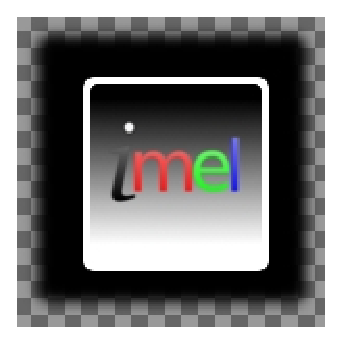
\includegraphics[width=\textwidth,height=\textheight/2,keepaspectratio=true]{images/imel_cutme}
\caption{Original Image}
\end{DoxyImage}

\begin{DoxyImage}
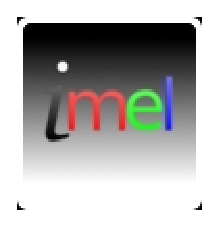
\includegraphics[width=\textwidth,height=\textheight/2,keepaspectratio=true]{images/auto_cut}
\caption{Image Result}
\end{DoxyImage}
 
\begin{DoxyParams}{Parameters}
{\em image} & Image to cut \\
\hline
{\em tollerance} & Tollerance for level or color to remove. \\
\hline
{\em reference} & Which type of cut do \\
\hline
{\em ...} & Level ( Imel\+Size ) or color ( Imel\+Pixel ) to remove from the sides. \\
\hline
\end{DoxyParams}
\begin{DoxyReturn}{Returns}
Cutted image.
\end{DoxyReturn}
\begin{DoxySeeAlso}{See also}
\hyperlink{image_8c_a54960c7fec6873dc13d2069d3c9eb718}{imel\+\_\+image\+\_\+cut} 

\hyperlink{image_8c_a31943792f957de747e49b6dc1fbbab05}{imel\+\_\+image\+\_\+cut\+\_\+grid} 

\hyperlink{header_8h_a6182c8947d12d828155f0fb8cb024209}{Imel\+Ref} 
\end{DoxySeeAlso}
\index{image.\+c@{image.\+c}!imel\+\_\+image\+\_\+change\+\_\+color\+\_\+level@{imel\+\_\+image\+\_\+change\+\_\+color\+\_\+level}}
\index{imel\+\_\+image\+\_\+change\+\_\+color\+\_\+level@{imel\+\_\+image\+\_\+change\+\_\+color\+\_\+level}!image.\+c@{image.\+c}}
\subsubsection[{\texorpdfstring{imel\+\_\+image\+\_\+change\+\_\+color\+\_\+level(\+Imel\+Image $\ast$image, Imel\+Level\+Operation level\+\_\+operation, Imel\+Level level, Imel\+Pixel color\+\_\+pxl, Imel\+Color tollerance)}{imel_image_change_color_level(ImelImage *image, ImelLevelOperation level_operation, ImelLevel level, ImelPixel color_pxl, ImelColor tollerance)}}]{\setlength{\rightskip}{0pt plus 5cm}void imel\+\_\+image\+\_\+change\+\_\+color\+\_\+level (
\begin{DoxyParamCaption}
\item[{{\bf Imel\+Image} $\ast$}]{image, }
\item[{{\bf Imel\+Level\+Operation}}]{level\+\_\+operation, }
\item[{{\bf Imel\+Level}}]{level, }
\item[{{\bf Imel\+Pixel}}]{color\+\_\+pxl, }
\item[{{\bf Imel\+Color}}]{tollerance}
\end{DoxyParamCaption}
)}\hypertarget{image_8c_a3e8526c34b3cb916894f09923ea2a116}{}\label{image_8c_a3e8526c34b3cb916894f09923ea2a116}


Change level to a specified color. 

This function change the level value for each {\ttfamily image} pixel that have a color equal or similar to {\ttfamily color\+\_\+pxl}.


\begin{DoxyParams}{Parameters}
{\em image} & Image to elaborate \\
\hline
{\em level\+\_\+operation} & Type of operation \\
\hline
{\em level} & New level or value for {\ttfamily level\+\_\+operation} \\
\hline
{\em color\+\_\+pxl} & Color to change the level \\
\hline
{\em tollerance} & Tollerance to find {\ttfamily color} \\
\hline
\end{DoxyParams}
\begin{DoxySeeAlso}{See also}
\hyperlink{header_8h_abece8958e8db1e2826f21fd822c14694}{Imel\+Level\+Operation} 

imel\+\_\+pixel\+\_\+compare 

\hyperlink{image_8c_a5fd7c413bcd1025d2c94810d66ba36eb}{imel\+\_\+image\+\_\+change\+\_\+level} 
\end{DoxySeeAlso}
\index{image.\+c@{image.\+c}!imel\+\_\+image\+\_\+change\+\_\+level@{imel\+\_\+image\+\_\+change\+\_\+level}}
\index{imel\+\_\+image\+\_\+change\+\_\+level@{imel\+\_\+image\+\_\+change\+\_\+level}!image.\+c@{image.\+c}}
\subsubsection[{\texorpdfstring{imel\+\_\+image\+\_\+change\+\_\+level(\+Imel\+Image $\ast$image, Imel\+Level\+Operation level\+\_\+operation, Imel\+Level level)}{imel_image_change_level(ImelImage *image, ImelLevelOperation level_operation, ImelLevel level)}}]{\setlength{\rightskip}{0pt plus 5cm}void imel\+\_\+image\+\_\+change\+\_\+level (
\begin{DoxyParamCaption}
\item[{{\bf Imel\+Image} $\ast$}]{image, }
\item[{{\bf Imel\+Level\+Operation}}]{level\+\_\+operation, }
\item[{{\bf Imel\+Level}}]{level}
\end{DoxyParamCaption}
)}\hypertarget{image_8c_a5fd7c413bcd1025d2c94810d66ba36eb}{}\label{image_8c_a5fd7c413bcd1025d2c94810d66ba36eb}


Change level of an image. 

This function change the level of {\ttfamily image}. It can be added or setted through the {\ttfamily level\+\_\+operation} argument.


\begin{DoxyParams}{Parameters}
{\em image} & Image to which change the level \\
\hline
{\em level\+\_\+operation} & Type of operation \\
\hline
{\em level} & New level or value for {\ttfamily level\+\_\+operation} \\
\hline
\end{DoxyParams}
\begin{DoxySeeAlso}{See also}
\hyperlink{header_8h_abece8958e8db1e2826f21fd822c14694}{Imel\+Level\+Operation} 

\hyperlink{image_8c_a3e8526c34b3cb916894f09923ea2a116}{imel\+\_\+image\+\_\+change\+\_\+color\+\_\+level} 
\end{DoxySeeAlso}
\index{image.\+c@{image.\+c}!imel\+\_\+image\+\_\+copy@{imel\+\_\+image\+\_\+copy}}
\index{imel\+\_\+image\+\_\+copy@{imel\+\_\+image\+\_\+copy}!image.\+c@{image.\+c}}
\subsubsection[{\texorpdfstring{imel\+\_\+image\+\_\+copy(\+Imel\+Image $\ast$image)}{imel_image_copy(ImelImage *image)}}]{\setlength{\rightskip}{0pt plus 5cm}{\bf Imel\+Image}$\ast$ imel\+\_\+image\+\_\+copy (
\begin{DoxyParamCaption}
\item[{{\bf Imel\+Image} $\ast$}]{image}
\end{DoxyParamCaption}
)}\hypertarget{image_8c_a8d41302f949cde87f3741455b3b9c23d}{}\label{image_8c_a8d41302f949cde87f3741455b3b9c23d}


Duplicate an image. 

This function copy {\ttfamily image} passed in a new one.


\begin{DoxyParams}{Parameters}
{\em image} & Image to copy \\
\hline
\end{DoxyParams}
\begin{DoxyReturn}{Returns}
A new Imel\+Image equal to {\ttfamily image} 
\end{DoxyReturn}
\index{image.\+c@{image.\+c}!imel\+\_\+image\+\_\+cut@{imel\+\_\+image\+\_\+cut}}
\index{imel\+\_\+image\+\_\+cut@{imel\+\_\+image\+\_\+cut}!image.\+c@{image.\+c}}
\subsubsection[{\texorpdfstring{imel\+\_\+image\+\_\+cut(\+Imel\+Image $\ast$image, Imel\+Size sx, Imel\+Size sy, Imel\+Size ex, Imel\+Size ey)}{imel_image_cut(ImelImage *image, ImelSize sx, ImelSize sy, ImelSize ex, ImelSize ey)}}]{\setlength{\rightskip}{0pt plus 5cm}{\bf Imel\+Image}$\ast$ imel\+\_\+image\+\_\+cut (
\begin{DoxyParamCaption}
\item[{{\bf Imel\+Image} $\ast$}]{image, }
\item[{{\bf Imel\+Size}}]{sx, }
\item[{{\bf Imel\+Size}}]{sy, }
\item[{{\bf Imel\+Size}}]{ex, }
\item[{{\bf Imel\+Size}}]{ey}
\end{DoxyParamCaption}
)}\hypertarget{image_8c_a54960c7fec6873dc13d2069d3c9eb718}{}\label{image_8c_a54960c7fec6873dc13d2069d3c9eb718}


Cut an image. 

This function cuts {\ttfamily image} from the coordinate {\ttfamily sx}, {\ttfamily sy} to the coordinate {\ttfamily ex}, {\ttfamily ey}.


\begin{DoxyParams}{Parameters}
{\em image} & Image to cut \\
\hline
{\em sx} & Start x coordinate \\
\hline
{\em sy} & Start y coordinate \\
\hline
{\em ex} & End x coordinate \\
\hline
{\em ey} & End y coordinate \\
\hline
\end{DoxyParams}
\begin{DoxyReturn}{Returns}
A new image with the {\ttfamily image} cutted 
\end{DoxyReturn}
\begin{DoxySeeAlso}{See also}
\hyperlink{image_8c_a75fbdaa484f8b191b8988af68181c488}{imel\+\_\+image\+\_\+auto\+\_\+cut} 

\hyperlink{image_8c_a31943792f957de747e49b6dc1fbbab05}{imel\+\_\+image\+\_\+cut\+\_\+grid} 
\end{DoxySeeAlso}
\index{image.\+c@{image.\+c}!imel\+\_\+image\+\_\+cut\+\_\+grid@{imel\+\_\+image\+\_\+cut\+\_\+grid}}
\index{imel\+\_\+image\+\_\+cut\+\_\+grid@{imel\+\_\+image\+\_\+cut\+\_\+grid}!image.\+c@{image.\+c}}
\subsubsection[{\texorpdfstring{imel\+\_\+image\+\_\+cut\+\_\+grid(\+Imel\+Image $\ast$image, Imel\+Info\+Cut $\ast$cut\+\_\+info)}{imel_image_cut_grid(ImelImage *image, ImelInfoCut *cut_info)}}]{\setlength{\rightskip}{0pt plus 5cm}{\bf Imel\+Image}$\ast$$\ast$ imel\+\_\+image\+\_\+cut\+\_\+grid (
\begin{DoxyParamCaption}
\item[{{\bf Imel\+Image} $\ast$}]{image, }
\item[{{\bf Imel\+Info\+Cut} $\ast$}]{cut\+\_\+info}
\end{DoxyParamCaption}
)}\hypertarget{image_8c_a31943792f957de747e49b6dc1fbbab05}{}\label{image_8c_a31943792f957de747e49b6dc1fbbab05}


Cut an image in more images. 

This function cut {\ttfamily image} in more images through a guide lines passed as {\ttfamily cut\+\_\+info}.


\begin{DoxyCode}
1 ImelImage *image = imel\_image\_new\_from ("cut\_orig.jpg", 0, NULL);
2 ImelImage **tiles;
3 ImelInfoCut *cut\_info;
4 int j;
5 
6 cut\_info = imel\_info\_cut\_new (IMEL\_ORIENTATION\_HORIZONTAL, 35);
7 cut\_info = imel\_info\_cut\_add (cut\_info, IMEL\_ORIENTATION\_HORIZONTAL, image->height - 35);
8 cut\_info = imel\_info\_cut\_add (cut\_info, IMEL\_ORIENTATION\_VERTICAL, 35);
9 cut\_info = imel\_info\_cut\_add (cut\_info, IMEL\_ORIENTATION\_VERTICAL, image->width - 35);
10 
11 tiles = imel\_image\_cut\_grid (image, cut\_info);
12 imel\_info\_cut\_free (cut\_info);
13 imel\_image\_free (image);
14 ...
15 for ( j = 0; tiles[j]; imel\_image\_free (tiles[j]), j++ );
16 free (tiles);
\end{DoxyCode}
 
\begin{DoxyImage}

\includegraphics[width=\textwidth,height=\textheight/2,keepaspectratio=true]{images/cut_orig}
\caption{Original Image}
\end{DoxyImage}

\begin{DoxyImage}

\includegraphics[width=\textwidth,height=\textheight/2,keepaspectratio=true]{images/cut_result}
\caption{Result Images}
\end{DoxyImage}
 
\begin{DoxyParams}{Parameters}
{\em image} & Image to cut \\
\hline
{\em cut\+\_\+info} & guide lines \\
\hline
\end{DoxyParams}
\begin{DoxyReturn}{Returns}
Cutted images in order inverse ( column, row ) inside a N\+U\+L\+L-\/terminated L\+I\+FO array.
\end{DoxyReturn}
\begin{DoxySeeAlso}{See also}
\hyperlink{image_8c_a54960c7fec6873dc13d2069d3c9eb718}{imel\+\_\+image\+\_\+cut} 

\hyperlink{image_8c_a75fbdaa484f8b191b8988af68181c488}{imel\+\_\+image\+\_\+auto\+\_\+cut} 

\hyperlink{info__cut_8c_ad06ec44d23c494c1f501d03de880007e}{imel\+\_\+info\+\_\+cut\+\_\+new} 

\hyperlink{info__cut_8c_aa8e34152e2f5716e6a195ee1b8107f85}{imel\+\_\+info\+\_\+cut\+\_\+add} 

\hyperlink{info__cut_8c_a73ba0a29544436cf4248c71a935560cd}{imel\+\_\+info\+\_\+cut\+\_\+free} 

\hyperlink{header_8h_aef27fcac7a96d118b3c3194c2577049f}{Imel\+Orientation} 
\end{DoxySeeAlso}
\index{image.\+c@{image.\+c}!imel\+\_\+image\+\_\+free@{imel\+\_\+image\+\_\+free}}
\index{imel\+\_\+image\+\_\+free@{imel\+\_\+image\+\_\+free}!image.\+c@{image.\+c}}
\subsubsection[{\texorpdfstring{imel\+\_\+image\+\_\+free(\+Imel\+Image $\ast$image)}{imel_image_free(ImelImage *image)}}]{\setlength{\rightskip}{0pt plus 5cm}void imel\+\_\+image\+\_\+free (
\begin{DoxyParamCaption}
\item[{{\bf Imel\+Image} $\ast$}]{image}
\end{DoxyParamCaption}
)}\hypertarget{image_8c_a873cba98c6f4f28e1db2bdf5da3cbfdd}{}\label{image_8c_a873cba98c6f4f28e1db2bdf5da3cbfdd}


Free an image. 

This function free memory allocated by {\ttfamily image}.


\begin{DoxyParams}{Parameters}
{\em image} & Image to free \\
\hline
\end{DoxyParams}
\index{image.\+c@{image.\+c}!imel\+\_\+image\+\_\+get\+\_\+height@{imel\+\_\+image\+\_\+get\+\_\+height}}
\index{imel\+\_\+image\+\_\+get\+\_\+height@{imel\+\_\+image\+\_\+get\+\_\+height}!image.\+c@{image.\+c}}
\subsubsection[{\texorpdfstring{imel\+\_\+image\+\_\+get\+\_\+height(\+Imel\+Image $\ast$image)}{imel_image_get_height(ImelImage *image)}}]{\setlength{\rightskip}{0pt plus 5cm}{\bf Imel\+Size} imel\+\_\+image\+\_\+get\+\_\+height (
\begin{DoxyParamCaption}
\item[{{\bf Imel\+Image} $\ast$}]{image}
\end{DoxyParamCaption}
)}\hypertarget{image_8c_acb0158f7e2714802231d7beb651ec47d}{}\label{image_8c_acb0158f7e2714802231d7beb651ec47d}


Get image height. 

This function get {\ttfamily image} height.


\begin{DoxyParams}{Parameters}
{\em image} & Image from which get the height \\
\hline
\end{DoxyParams}
\begin{DoxyReturn}{Returns}
{\ttfamily image} height 
\end{DoxyReturn}
\begin{DoxyNote}{Note}
Same as {\ttfamily image-\/$>$height} 
\end{DoxyNote}
\index{image.\+c@{image.\+c}!imel\+\_\+image\+\_\+get\+\_\+histogram@{imel\+\_\+image\+\_\+get\+\_\+histogram}}
\index{imel\+\_\+image\+\_\+get\+\_\+histogram@{imel\+\_\+image\+\_\+get\+\_\+histogram}!image.\+c@{image.\+c}}
\subsubsection[{\texorpdfstring{imel\+\_\+image\+\_\+get\+\_\+histogram(\+Imel\+Image $\ast$image, Imel\+Histogram histogram\+\_\+type)}{imel_image_get_histogram(ImelImage *image, ImelHistogram histogram_type)}}]{\setlength{\rightskip}{0pt plus 5cm}int$\ast$ imel\+\_\+image\+\_\+get\+\_\+histogram (
\begin{DoxyParamCaption}
\item[{{\bf Imel\+Image} $\ast$}]{image, }
\item[{{\bf Imel\+Histogram}}]{histogram\+\_\+type}
\end{DoxyParamCaption}
)}\hypertarget{image_8c_afa2cd389929358c87f2d21e1e7b2ef9a}{}\label{image_8c_afa2cd389929358c87f2d21e1e7b2ef9a}


Get histogram values from an image. 

This function get the histogram values from {\ttfamily image} for {\ttfamily histogram\+\_\+type} chosen.


\begin{DoxyParams}{Parameters}
{\em image} & Image from which get the values \\
\hline
{\em histogram\+\_\+type} & Types of values to get \\
\hline
\end{DoxyParams}
\begin{DoxyReturn}{Returns}
An array with 256 element
\end{DoxyReturn}
\begin{DoxySeeAlso}{See also}
\hyperlink{header_8h_a8879c5e403ddb26c326b1cc2c3e529bf}{Imel\+Histogram} 

\hyperlink{image_8c_ae416e85c63ce2f3f60df3fb31c5d41b5}{imel\+\_\+image\+\_\+get\+\_\+histogram\+\_\+image} 

\hyperlink{image_8c_a41cc4f146e4863e1969bfa15ca3e7afc}{imel\+\_\+image\+\_\+get\+\_\+histograms\+\_\+image} 
\end{DoxySeeAlso}
\index{image.\+c@{image.\+c}!imel\+\_\+image\+\_\+get\+\_\+histogram\+\_\+image@{imel\+\_\+image\+\_\+get\+\_\+histogram\+\_\+image}}
\index{imel\+\_\+image\+\_\+get\+\_\+histogram\+\_\+image@{imel\+\_\+image\+\_\+get\+\_\+histogram\+\_\+image}!image.\+c@{image.\+c}}
\subsubsection[{\texorpdfstring{imel\+\_\+image\+\_\+get\+\_\+histogram\+\_\+image(\+Imel\+Image $\ast$image, int $\ast$\+\_\+\+\_\+histogram, Imel\+Histogram histogram\+\_\+type)}{imel_image_get_histogram_image(ImelImage *image, int *__histogram, ImelHistogram histogram_type)}}]{\setlength{\rightskip}{0pt plus 5cm}{\bf Imel\+Image}$\ast$ imel\+\_\+image\+\_\+get\+\_\+histogram\+\_\+image (
\begin{DoxyParamCaption}
\item[{{\bf Imel\+Image} $\ast$}]{image, }
\item[{int $\ast$}]{\+\_\+\+\_\+histogram, }
\item[{{\bf Imel\+Histogram}}]{histogram\+\_\+type}
\end{DoxyParamCaption}
)}\hypertarget{image_8c_ae416e85c63ce2f3f60df3fb31c5d41b5}{}\label{image_8c_ae416e85c63ce2f3f60df3fb31c5d41b5}


Make an histogram image for an image chosen. 

This function make an histogram for {\ttfamily image} from which are already elaborated the values through \hyperlink{image_8c_afa2cd389929358c87f2d21e1e7b2ef9a}{imel\+\_\+image\+\_\+get\+\_\+histogram} () function.


\begin{DoxyImage}
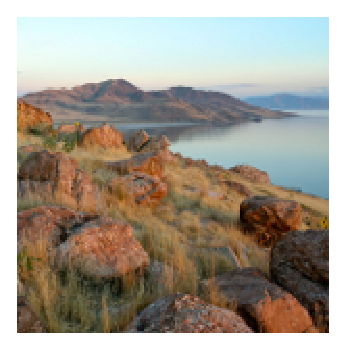
\includegraphics[width=\textwidth,height=\textheight/2,keepaspectratio=true]{images/histogram_me}
\caption{Original Image}
\end{DoxyImage}

\begin{DoxyImage}
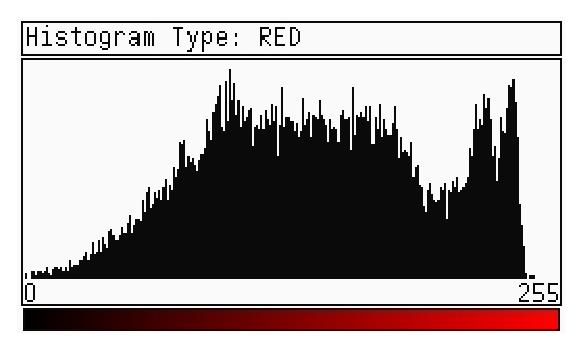
\includegraphics[width=\textwidth,height=\textheight/2,keepaspectratio=true]{images/histogram}
\caption{Output Image}
\end{DoxyImage}
 
\begin{DoxyParams}{Parameters}
{\em image} & Image from which get the histogram \\
\hline
{\em \+\_\+\+\_\+histogram} & Values returned from imel\+\_\+image\+\_\+get\+\_\+histogram () function \\
\hline
{\em histogram\+\_\+type} & Histogram type. \\
\hline
\end{DoxyParams}
\begin{DoxyReturn}{Returns}
Histogram image
\end{DoxyReturn}
\begin{DoxySeeAlso}{See also}
\hyperlink{header_8h_a8879c5e403ddb26c326b1cc2c3e529bf}{Imel\+Histogram} 

\hyperlink{image_8c_afa2cd389929358c87f2d21e1e7b2ef9a}{imel\+\_\+image\+\_\+get\+\_\+histogram} 

\hyperlink{image_8c_a41cc4f146e4863e1969bfa15ca3e7afc}{imel\+\_\+image\+\_\+get\+\_\+histograms\+\_\+image} 
\end{DoxySeeAlso}
\index{image.\+c@{image.\+c}!imel\+\_\+image\+\_\+get\+\_\+histograms\+\_\+image@{imel\+\_\+image\+\_\+get\+\_\+histograms\+\_\+image}}
\index{imel\+\_\+image\+\_\+get\+\_\+histograms\+\_\+image@{imel\+\_\+image\+\_\+get\+\_\+histograms\+\_\+image}!image.\+c@{image.\+c}}
\subsubsection[{\texorpdfstring{imel\+\_\+image\+\_\+get\+\_\+histograms\+\_\+image(\+Imel\+Image $\ast$image, Imel\+Histogram\+Layout layout)}{imel_image_get_histograms_image(ImelImage *image, ImelHistogramLayout layout)}}]{\setlength{\rightskip}{0pt plus 5cm}{\bf Imel\+Image}$\ast$ imel\+\_\+image\+\_\+get\+\_\+histograms\+\_\+image (
\begin{DoxyParamCaption}
\item[{{\bf Imel\+Image} $\ast$}]{image, }
\item[{{\bf Imel\+Histogram\+Layout}}]{layout}
\end{DoxyParamCaption}
)}\hypertarget{image_8c_a41cc4f146e4863e1969bfa15ca3e7afc}{}\label{image_8c_a41cc4f146e4863e1969bfa15ca3e7afc}


Make all types of histogram of an image. 

This function make all types of histogram of {\ttfamily image} with a chosen {\ttfamily layout}.

 
\begin{DoxyImageNoCaption}
  \mbox{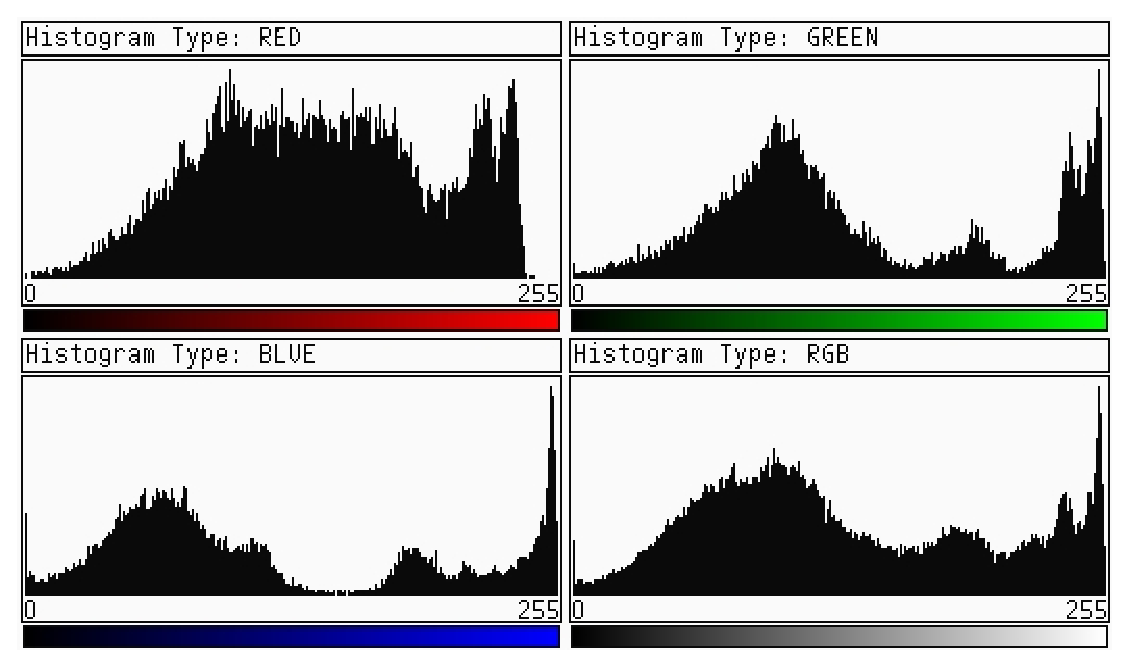
\includegraphics[width=\textwidth,height=\textheight/2,keepaspectratio=true]{images/histogram_panels}}
\end{DoxyImageNoCaption}



\begin{DoxyParams}{Parameters}
{\em image} & Image from which get histograms \\
\hline
{\em layout} & Layout of the histograms \\
\hline
\end{DoxyParams}
\begin{DoxyReturn}{Returns}
The image with all the histograms
\end{DoxyReturn}
\begin{DoxySeeAlso}{See also}
\hyperlink{header_8h_aacf376be43512b219081df71ed7ee438}{Imel\+Histogram\+Layout} 

\hyperlink{image_8c_afa2cd389929358c87f2d21e1e7b2ef9a}{imel\+\_\+image\+\_\+get\+\_\+histogram} 

\hyperlink{image_8c_ae416e85c63ce2f3f60df3fb31c5d41b5}{imel\+\_\+image\+\_\+get\+\_\+histogram\+\_\+image} 
\end{DoxySeeAlso}
\index{image.\+c@{image.\+c}!imel\+\_\+image\+\_\+get\+\_\+width@{imel\+\_\+image\+\_\+get\+\_\+width}}
\index{imel\+\_\+image\+\_\+get\+\_\+width@{imel\+\_\+image\+\_\+get\+\_\+width}!image.\+c@{image.\+c}}
\subsubsection[{\texorpdfstring{imel\+\_\+image\+\_\+get\+\_\+width(\+Imel\+Image $\ast$image)}{imel_image_get_width(ImelImage *image)}}]{\setlength{\rightskip}{0pt plus 5cm}{\bf Imel\+Size} imel\+\_\+image\+\_\+get\+\_\+width (
\begin{DoxyParamCaption}
\item[{{\bf Imel\+Image} $\ast$}]{image}
\end{DoxyParamCaption}
)}\hypertarget{image_8c_a203143cba24be50f6d48eb50bcf64459}{}\label{image_8c_a203143cba24be50f6d48eb50bcf64459}


Get image width. 

This function get {\ttfamily image} width.


\begin{DoxyParams}{Parameters}
{\em image} & Image from which get the width \\
\hline
\end{DoxyParams}
\begin{DoxyReturn}{Returns}
{\ttfamily image} width 
\end{DoxyReturn}
\begin{DoxyNote}{Note}
Same as {\ttfamily image-\/$>$width} 
\end{DoxyNote}
\index{image.\+c@{image.\+c}!imel\+\_\+image\+\_\+insert\+\_\+image@{imel\+\_\+image\+\_\+insert\+\_\+image}}
\index{imel\+\_\+image\+\_\+insert\+\_\+image@{imel\+\_\+image\+\_\+insert\+\_\+image}!image.\+c@{image.\+c}}
\subsubsection[{\texorpdfstring{imel\+\_\+image\+\_\+insert\+\_\+image(\+Imel\+Image $\ast$dest, Imel\+Image $\ast$src, Imel\+Size sx, Imel\+Size sy)}{imel_image_insert_image(ImelImage *dest, ImelImage *src, ImelSize sx, ImelSize sy)}}]{\setlength{\rightskip}{0pt plus 5cm}void imel\+\_\+image\+\_\+insert\+\_\+image (
\begin{DoxyParamCaption}
\item[{{\bf Imel\+Image} $\ast$}]{dest, }
\item[{{\bf Imel\+Image} $\ast$}]{src, }
\item[{{\bf Imel\+Size}}]{sx, }
\item[{{\bf Imel\+Size}}]{sy}
\end{DoxyParamCaption}
)}\hypertarget{image_8c_acdefba6da2457b909d9ca2600a13bc65}{}\label{image_8c_acdefba6da2457b909d9ca2600a13bc65}


Insert an image in another one. 

This function insert the image {\ttfamily src} in the image {\ttfamily dest} from position $(sx,sy)$.


\begin{DoxyParams}{Parameters}
{\em dest} & Destination image \\
\hline
{\em src} & Image to insert in {\ttfamily dest} \\
\hline
{\em sx} & Start x coordinate \\
\hline
{\em sy} & Start y coordinate\\
\hline
\end{DoxyParams}
\begin{DoxyNote}{Note}
This function uses indirectly \hyperlink{pixel_8c_a9bc6aa8b3ec663f1635827b0ebbdf46a}{imel\+\_\+pixel\+\_\+copy} () function to insert {\ttfamily src} in {\ttfamily dest} 
\end{DoxyNote}
\begin{DoxySeeAlso}{See also}
\hyperlink{pixel_8c_a9bc6aa8b3ec663f1635827b0ebbdf46a}{imel\+\_\+pixel\+\_\+copy} 

\hyperlink{image_8c_a12519cad063897a1dcf9eb4c677b8304}{imel\+\_\+image\+\_\+union} 
\end{DoxySeeAlso}
\index{image.\+c@{image.\+c}!imel\+\_\+image\+\_\+mirror\+\_\+horizontal@{imel\+\_\+image\+\_\+mirror\+\_\+horizontal}}
\index{imel\+\_\+image\+\_\+mirror\+\_\+horizontal@{imel\+\_\+image\+\_\+mirror\+\_\+horizontal}!image.\+c@{image.\+c}}
\subsubsection[{\texorpdfstring{imel\+\_\+image\+\_\+mirror\+\_\+horizontal(\+Imel\+Image $\ast$image)}{imel_image_mirror_horizontal(ImelImage *image)}}]{\setlength{\rightskip}{0pt plus 5cm}{\bf Imel\+Image}$\ast$ imel\+\_\+image\+\_\+mirror\+\_\+horizontal (
\begin{DoxyParamCaption}
\item[{{\bf Imel\+Image} $\ast$}]{image}
\end{DoxyParamCaption}
)}\hypertarget{image_8c_a4a2cd319143d8bcc9cd60cc191713664}{}\label{image_8c_a4a2cd319143d8bcc9cd60cc191713664}


Mirror an image to horizontal. 

This function applies the mirror horizontal effect to {\ttfamily image}.


\begin{DoxyParams}{Parameters}
{\em image} & Image to mirror \\
\hline
\end{DoxyParams}
\begin{DoxyReturn}{Returns}
A copy of {\ttfamily image} mirrored horizontally 
\end{DoxyReturn}
\begin{DoxySeeAlso}{See also}
\hyperlink{image_8c_a9e7cf1420d1937b0528104da21bab4c2}{imel\+\_\+image\+\_\+mirror\+\_\+vertical} 
\end{DoxySeeAlso}
\index{image.\+c@{image.\+c}!imel\+\_\+image\+\_\+mirror\+\_\+vertical@{imel\+\_\+image\+\_\+mirror\+\_\+vertical}}
\index{imel\+\_\+image\+\_\+mirror\+\_\+vertical@{imel\+\_\+image\+\_\+mirror\+\_\+vertical}!image.\+c@{image.\+c}}
\subsubsection[{\texorpdfstring{imel\+\_\+image\+\_\+mirror\+\_\+vertical(\+Imel\+Image $\ast$image)}{imel_image_mirror_vertical(ImelImage *image)}}]{\setlength{\rightskip}{0pt plus 5cm}{\bf Imel\+Image}$\ast$ imel\+\_\+image\+\_\+mirror\+\_\+vertical (
\begin{DoxyParamCaption}
\item[{{\bf Imel\+Image} $\ast$}]{image}
\end{DoxyParamCaption}
)}\hypertarget{image_8c_a9e7cf1420d1937b0528104da21bab4c2}{}\label{image_8c_a9e7cf1420d1937b0528104da21bab4c2}


Mirror an image to vertical. 

This function applies the mirror vertical effect to {\ttfamily image}.


\begin{DoxyParams}{Parameters}
{\em image} & Image to mirror \\
\hline
\end{DoxyParams}
\begin{DoxyReturn}{Returns}
A copy of {\ttfamily image} mirrored vertically 
\end{DoxyReturn}
\begin{DoxySeeAlso}{See also}
\hyperlink{image_8c_a4a2cd319143d8bcc9cd60cc191713664}{imel\+\_\+image\+\_\+mirror\+\_\+horizontal} 
\end{DoxySeeAlso}
\index{image.\+c@{image.\+c}!imel\+\_\+image\+\_\+new@{imel\+\_\+image\+\_\+new}}
\index{imel\+\_\+image\+\_\+new@{imel\+\_\+image\+\_\+new}!image.\+c@{image.\+c}}
\subsubsection[{\texorpdfstring{imel\+\_\+image\+\_\+new(\+Imel\+Size width, Imel\+Size height)}{imel_image_new(ImelSize width, ImelSize height)}}]{\setlength{\rightskip}{0pt plus 5cm}{\bf Imel\+Image}$\ast$ imel\+\_\+image\+\_\+new (
\begin{DoxyParamCaption}
\item[{{\bf Imel\+Size}}]{width, }
\item[{{\bf Imel\+Size}}]{height}
\end{DoxyParamCaption}
)}\hypertarget{image_8c_af3a4abcb52f5611781065536fda0f97e}{}\label{image_8c_af3a4abcb52f5611781065536fda0f97e}


Make a new image. 

This function make a new image with black background and level set to -\/255.


\begin{DoxyParams}{Parameters}
{\em width} & Image width \\
\hline
{\em height} & Image height \\
\hline
\end{DoxyParams}
\begin{DoxyReturn}{Returns}
A new Imel\+Image or N\+U\+LL on error
\end{DoxyReturn}
\begin{DoxySeeAlso}{See also}
\hyperlink{image_8c_a4692c85413196d5e15149cf4c66e1f08}{imel\+\_\+image\+\_\+new\+\_\+with\+\_\+background\+\_\+color} 
\end{DoxySeeAlso}
\index{image.\+c@{image.\+c}!imel\+\_\+image\+\_\+new\+\_\+with\+\_\+background\+\_\+color@{imel\+\_\+image\+\_\+new\+\_\+with\+\_\+background\+\_\+color}}
\index{imel\+\_\+image\+\_\+new\+\_\+with\+\_\+background\+\_\+color@{imel\+\_\+image\+\_\+new\+\_\+with\+\_\+background\+\_\+color}!image.\+c@{image.\+c}}
\subsubsection[{\texorpdfstring{imel\+\_\+image\+\_\+new\+\_\+with\+\_\+background\+\_\+color(\+Imel\+Size width, Imel\+Size height, Imel\+Pixel pixel)}{imel_image_new_with_background_color(ImelSize width, ImelSize height, ImelPixel pixel)}}]{\setlength{\rightskip}{0pt plus 5cm}{\bf Imel\+Image}$\ast$ imel\+\_\+image\+\_\+new\+\_\+with\+\_\+background\+\_\+color (
\begin{DoxyParamCaption}
\item[{{\bf Imel\+Size}}]{width, }
\item[{{\bf Imel\+Size}}]{height, }
\item[{{\bf Imel\+Pixel}}]{pixel}
\end{DoxyParamCaption}
)}\hypertarget{image_8c_a4692c85413196d5e15149cf4c66e1f08}{}\label{image_8c_a4692c85413196d5e15149cf4c66e1f08}


Make a new image with background color and level specified. 

This function make a new image which each pixel is set to {\ttfamily pixel} passed.


\begin{DoxyParams}{Parameters}
{\em width} & Image width \\
\hline
{\em height} & Image height \\
\hline
{\em pixel} & Color and level of the image \\
\hline
\end{DoxyParams}
\begin{DoxyReturn}{Returns}
a new Imel\+Image
\end{DoxyReturn}
\begin{DoxySeeAlso}{See also}
\hyperlink{image_8c_af3a4abcb52f5611781065536fda0f97e}{imel\+\_\+image\+\_\+new} 
\end{DoxySeeAlso}
\index{image.\+c@{image.\+c}!imel\+\_\+image\+\_\+perspective@{imel\+\_\+image\+\_\+perspective}}
\index{imel\+\_\+image\+\_\+perspective@{imel\+\_\+image\+\_\+perspective}!image.\+c@{image.\+c}}
\subsubsection[{\texorpdfstring{imel\+\_\+image\+\_\+perspective(\+Imel\+Image $\ast$image, double rad\+\_\+angle, Imel\+Orientation orientation)}{imel_image_perspective(ImelImage *image, double rad_angle, ImelOrientation orientation)}}]{\setlength{\rightskip}{0pt plus 5cm}{\bf Imel\+Image}$\ast$ imel\+\_\+image\+\_\+perspective (
\begin{DoxyParamCaption}
\item[{{\bf Imel\+Image} $\ast$}]{image, }
\item[{double}]{rad\+\_\+angle, }
\item[{{\bf Imel\+Orientation}}]{orientation}
\end{DoxyParamCaption}
)}\hypertarget{image_8c_ad08c629d2c44d24e7c485b7ff9a28021}{}\label{image_8c_ad08c629d2c44d24e7c485b7ff9a28021}


Makes an horizontal or vertical perspective. 

This function makes a perspective horizontal or vertical with a certain angle.


\begin{DoxyCode}
1 ImelImage *src = imel\_image\_new\_from ("butterfly.jpg", 0, NULL);
2 ImelImage **p;
3 
4 p = imel\_image\_perspective (src, 0.785398, IMEL\_ORIENTATION\_HORIZONTAL);
5 ...
6 p = imel\_image\_perspective (src, -0.785398, IMEL\_ORIENTATION\_HORIZONTAL);
7 ...
8 p = imel\_image\_perspective (src, 0.785398, IMEL\_ORIENTATION\_VERTICAL);
9 ...
10 p = imel\_image\_perspective (src, -0.785398, IMEL\_ORIENTATION\_VERTICAL);
\end{DoxyCode}
 
\begin{DoxyImage}
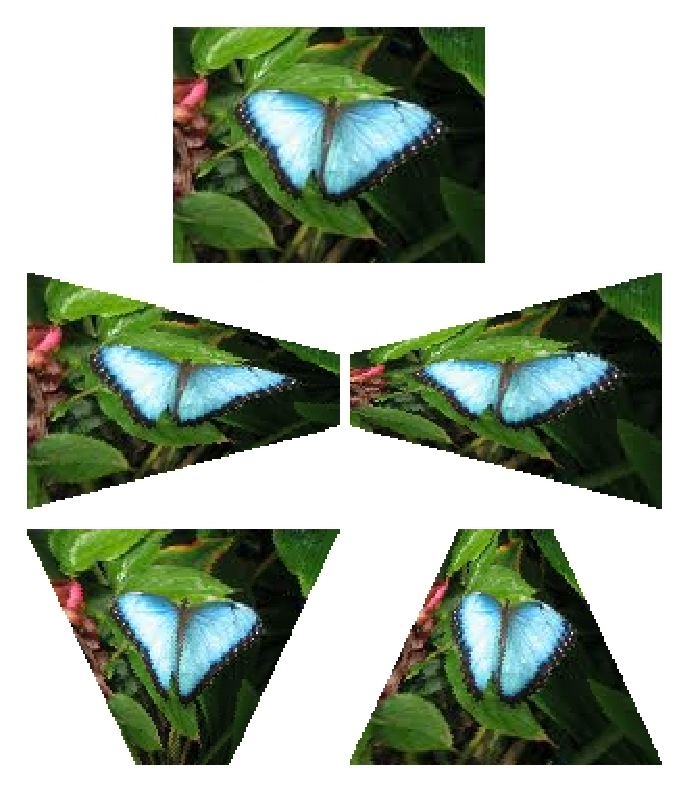
\includegraphics[width=\textwidth,height=\textheight/2,keepaspectratio=true]{images/perspective}
\caption{Example}
\end{DoxyImage}

\begin{DoxyParams}{Parameters}
{\em image} & Original image \\
\hline
{\em rad\+\_\+angle} & Perspective angle in radians. \\
\hline
{\em orientation} & Perspective type. \\
\hline
\end{DoxyParams}
\begin{DoxyReturn}{Returns}
A new image with the effect applied. 
\end{DoxyReturn}
\begin{DoxySeeAlso}{See also}
\hyperlink{header_8h_aef27fcac7a96d118b3c3194c2577049f}{Imel\+Orientation} 

\hyperlink{image_8c_aa517733f37a96bfcccf4ee666a92b206}{imel\+\_\+image\+\_\+slant} 
\end{DoxySeeAlso}
\index{image.\+c@{image.\+c}!imel\+\_\+image\+\_\+remove\+\_\+base\+\_\+color@{imel\+\_\+image\+\_\+remove\+\_\+base\+\_\+color}}
\index{imel\+\_\+image\+\_\+remove\+\_\+base\+\_\+color@{imel\+\_\+image\+\_\+remove\+\_\+base\+\_\+color}!image.\+c@{image.\+c}}
\subsubsection[{\texorpdfstring{imel\+\_\+image\+\_\+remove\+\_\+base\+\_\+color(\+Imel\+Image $\ast$image, Imel\+Mask mask)}{imel_image_remove_base_color(ImelImage *image, ImelMask mask)}}]{\setlength{\rightskip}{0pt plus 5cm}void imel\+\_\+image\+\_\+remove\+\_\+base\+\_\+color (
\begin{DoxyParamCaption}
\item[{{\bf Imel\+Image} $\ast$}]{image, }
\item[{{\bf Imel\+Mask}}]{mask}
\end{DoxyParamCaption}
)}\hypertarget{image_8c_ae2c499f2810e903a36b2b766541a815e}{}\label{image_8c_ae2c499f2810e903a36b2b766541a815e}


Remove a color. 

This function set to 0 the channel, or the channels, specified

This function set to 255 the channel, or the channels, specified as {\ttfamily mask}.


\begin{DoxyCode}
1 ImelImage *image = imel\_image\_new\_from ("image.jpg", 0, NULL);
2 
3 imel\_image\_remove\_base\_color (image, IMEL\_MASK\_RED | IMEL\_MASK\_BLUE);
\end{DoxyCode}



\begin{DoxyParams}{Parameters}
{\em image} & Image on which remove the color \\
\hline
{\em mask} & Channel, or channels, to set to 0. \\
\hline
\end{DoxyParams}
\begin{DoxySeeAlso}{See also}
\hyperlink{header_8h_a9facf73fdf3eb7434d01cd1c07341a28}{Imel\+Mask} 

\hyperlink{image_8c_abdb78af6d874ae54552a6f3219c75127}{imel\+\_\+image\+\_\+apply\+\_\+filter} 
\end{DoxySeeAlso}
\index{image.\+c@{image.\+c}!imel\+\_\+image\+\_\+remove\+\_\+noise@{imel\+\_\+image\+\_\+remove\+\_\+noise}}
\index{imel\+\_\+image\+\_\+remove\+\_\+noise@{imel\+\_\+image\+\_\+remove\+\_\+noise}!image.\+c@{image.\+c}}
\subsubsection[{\texorpdfstring{imel\+\_\+image\+\_\+remove\+\_\+noise(\+Imel\+Image $\ast$image, Imel\+Size size\+\_\+q, Imel\+Mask mask, Imel\+Color tollerance)}{imel_image_remove_noise(ImelImage *image, ImelSize size_q, ImelMask mask, ImelColor tollerance)}}]{\setlength{\rightskip}{0pt plus 5cm}void imel\+\_\+image\+\_\+remove\+\_\+noise (
\begin{DoxyParamCaption}
\item[{{\bf Imel\+Image} $\ast$}]{image, }
\item[{{\bf Imel\+Size}}]{size\+\_\+q, }
\item[{{\bf Imel\+Mask}}]{mask, }
\item[{{\bf Imel\+Color}}]{tollerance}
\end{DoxyParamCaption}
)}\hypertarget{image_8c_aedeae21c9710c31bf78b5a12d03a031f}{}\label{image_8c_aedeae21c9710c31bf78b5a12d03a031f}


Remove noise from an image. 

This function remove noise from {\ttfamily image}. Compare each pixel with all other around in a square with side {\ttfamily size\+\_\+q} pixel. If current pixel are a value greater then the average of others pixel compared, with a specified {\ttfamily tollerance}, change its value with the average found.


\begin{DoxyCode}
1 ImelImage *image = imel\_image\_new\_from ("apply\_noise.jpg", 0, NULL);
2 ImelMask mask = IMEL\_MASK\_RED | IMEL\_MASK\_GREEN | IMEL\_MASK\_BLUE;
3 
4 imel\_image\_remove\_noise (image, 6, mask, 24);
\end{DoxyCode}
 
\begin{DoxyImage}
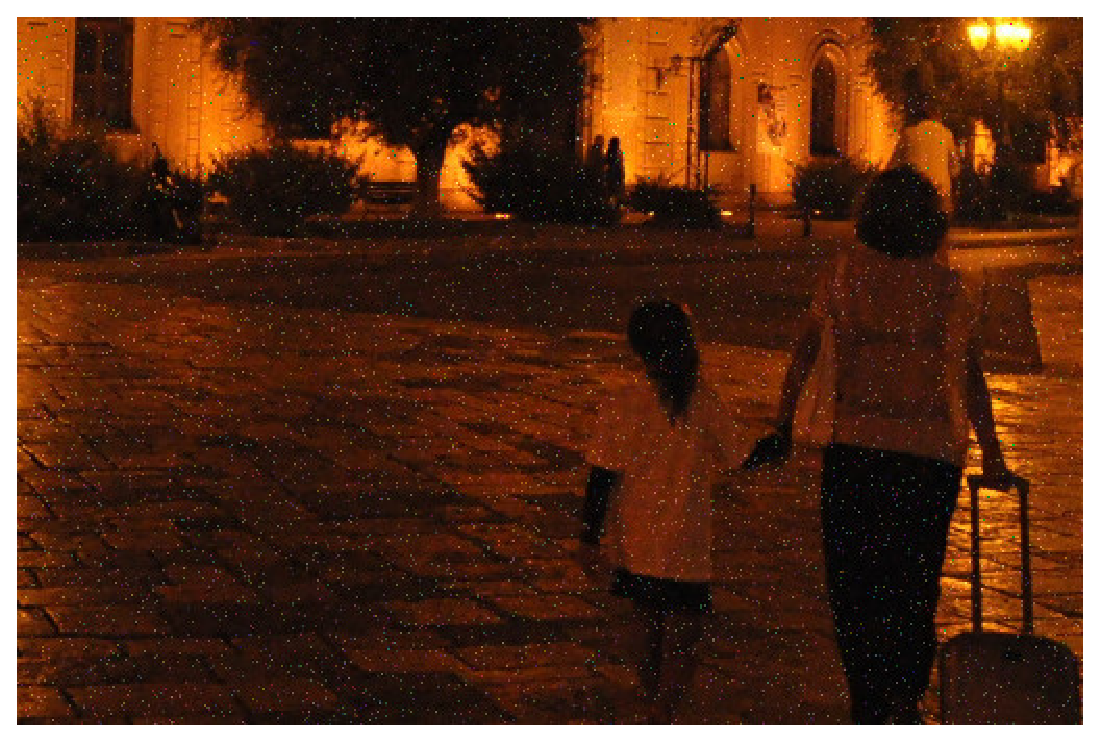
\includegraphics[width=\textwidth,height=\textheight/2,keepaspectratio=true]{images/apply_noise}
\caption{Input Image}
\end{DoxyImage}

\begin{DoxyImage}
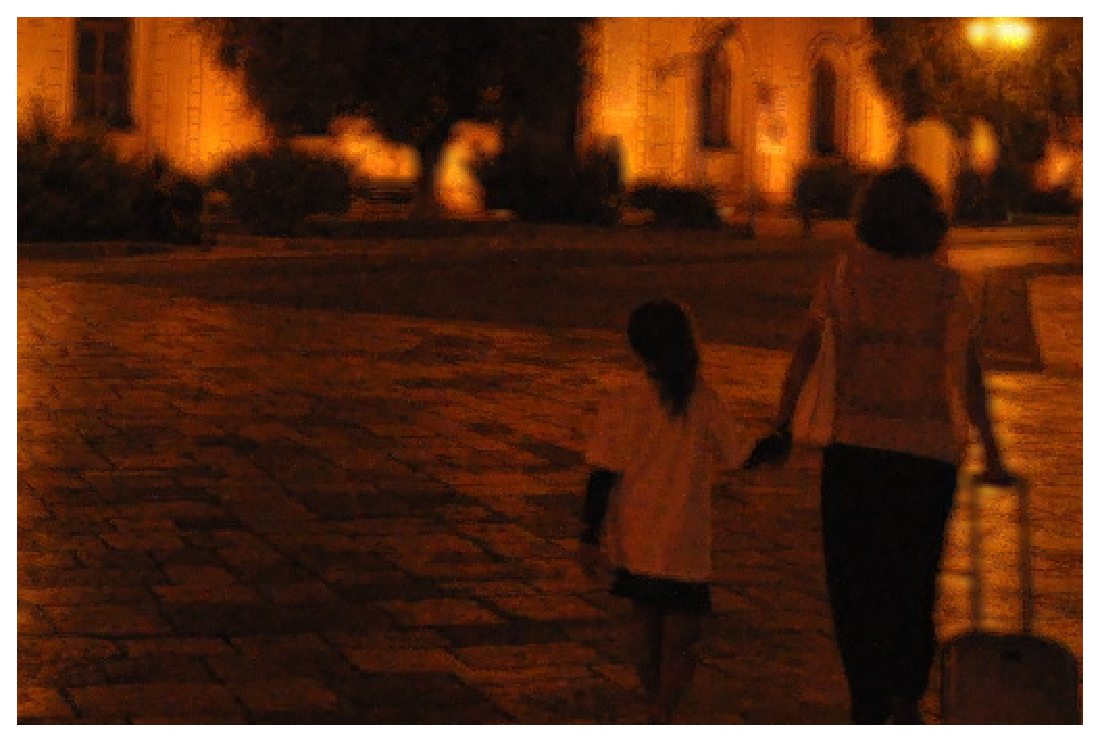
\includegraphics[width=\textwidth,height=\textheight/2,keepaspectratio=true]{images/remove_noise}
\caption{Result Image}
\end{DoxyImage}
 
\begin{DoxyParams}{Parameters}
{\em image} & Image with noise \\
\hline
{\em size\+\_\+q} & Size of the square side where the current pixel are. \\
\hline
{\em mask} & Channels affected from noise. \\
\hline
{\em tollerance} & Tollerance when compare current pixel with the average of others.\\
\hline
\end{DoxyParams}
\begin{DoxySeeAlso}{See also}
\hyperlink{image_8c_a5b3d70708a116076bfbcaeb7a9cd2b5d}{imel\+\_\+image\+\_\+apply\+\_\+noise} 
\end{DoxySeeAlso}
\index{image.\+c@{image.\+c}!imel\+\_\+image\+\_\+replace\+\_\+area\+\_\+color@{imel\+\_\+image\+\_\+replace\+\_\+area\+\_\+color}}
\index{imel\+\_\+image\+\_\+replace\+\_\+area\+\_\+color@{imel\+\_\+image\+\_\+replace\+\_\+area\+\_\+color}!image.\+c@{image.\+c}}
\subsubsection[{\texorpdfstring{imel\+\_\+image\+\_\+replace\+\_\+area\+\_\+color(\+Imel\+Image $\ast$image, Imel\+Pixel src, Imel\+Pixel dest, Imel\+Size tollerance, Imel\+Size \+\_\+x1, Imel\+Size \+\_\+y1, Imel\+Size \+\_\+x2, Imel\+Size \+\_\+y2)}{imel_image_replace_area_color(ImelImage *image, ImelPixel src, ImelPixel dest, ImelSize tollerance, ImelSize _x1, ImelSize _y1, ImelSize _x2, ImelSize _y2)}}]{\setlength{\rightskip}{0pt plus 5cm}void imel\+\_\+image\+\_\+replace\+\_\+area\+\_\+color (
\begin{DoxyParamCaption}
\item[{{\bf Imel\+Image} $\ast$}]{image, }
\item[{{\bf Imel\+Pixel}}]{src, }
\item[{{\bf Imel\+Pixel}}]{dest, }
\item[{{\bf Imel\+Size}}]{tollerance, }
\item[{{\bf Imel\+Size}}]{\+\_\+x1, }
\item[{{\bf Imel\+Size}}]{\+\_\+y1, }
\item[{{\bf Imel\+Size}}]{\+\_\+x2, }
\item[{{\bf Imel\+Size}}]{\+\_\+y2}
\end{DoxyParamCaption}
)}\hypertarget{image_8c_a59e0bc363c90fe9e002b1e93e66475e8}{}\label{image_8c_a59e0bc363c90fe9e002b1e93e66475e8}


Replace a color with an other one in a specified area. 

This function replace the pixel {\ttfamily src} with {\ttfamily desc} though \hyperlink{draw_8c_a80e6d667aceb3de202823e5493a774b1}{imel\+\_\+draw\+\_\+point} () in an area from coordinate $(\_x_1,\_y_1)$ to coordinate $(\_x_2,\_y_2)$ inside the {\ttfamily image}. The research of {\ttfamily src} in {\ttfamily image} will be done with a {\ttfamily tollerance} calculated in this function with \#imel\+\_\+pixel\+\_\+compare ().


\begin{DoxyCode}
1 ImelImage *image = imel\_image\_new\_from ("image.jpg", 0, NULL);
2 ImelPixel find = \{ 0xff, 0x66, 0x00, 0 \}, replace = \{ 0xff, 0x00, 0x00, 0 \};
3 ImelSize start[2], end[2];
4 
5 start[0] = image->width  / 2;
6 start[1] = image->height / 2;
7   end[0] = image->width  - start[0];
8   end[1] = image->height - start[1];
9 
10 imel\_image\_replace\_area\_color (image, find, replace, 16, start[0], start[1], end[0], end[1]);
\end{DoxyCode}
 
\begin{DoxyImage}

\includegraphics[width=\textwidth,height=\textheight/2,keepaspectratio=true]{images/pattern}
\caption{Original Image}
\end{DoxyImage}

\begin{DoxyImage}

\includegraphics[width=\textwidth,height=\textheight/2,keepaspectratio=true]{images/replace_area_color}
\caption{Example Output}
\end{DoxyImage}

\begin{DoxyParams}{Parameters}
{\em image} & Image where replace {\ttfamily src} with {\ttfamily dest} \\
\hline
{\em src} & Pixel to replace with {\ttfamily dest} \\
\hline
{\em dest} & New pixel for {\ttfamily src} occourrences. \\
\hline
{\em tollerance} & Tollerance for {\ttfamily src}. Values between 0 and 255. \\
\hline
{\em \+\_\+x1} & Start x coordinate \\
\hline
{\em \+\_\+y1} & Start y coordinate \\
\hline
{\em \+\_\+x2} & End x coordinate \\
\hline
{\em \+\_\+y2} & End y coordinate \\
\hline
\end{DoxyParams}
\begin{DoxySeeAlso}{See also}
\hyperlink{draw_8c_a80e6d667aceb3de202823e5493a774b1}{imel\+\_\+draw\+\_\+point} 

imel\+\_\+pixel\+\_\+compare 

\hyperlink{image_8c_a155f45bccd5beef204d410a7d399bc00}{imel\+\_\+image\+\_\+replace\+\_\+color} 
\end{DoxySeeAlso}
\index{image.\+c@{image.\+c}!imel\+\_\+image\+\_\+replace\+\_\+color@{imel\+\_\+image\+\_\+replace\+\_\+color}}
\index{imel\+\_\+image\+\_\+replace\+\_\+color@{imel\+\_\+image\+\_\+replace\+\_\+color}!image.\+c@{image.\+c}}
\subsubsection[{\texorpdfstring{imel\+\_\+image\+\_\+replace\+\_\+color(\+Imel\+Image $\ast$image, Imel\+Pixel src, Imel\+Pixel dest, Imel\+Size tollerance)}{imel_image_replace_color(ImelImage *image, ImelPixel src, ImelPixel dest, ImelSize tollerance)}}]{\setlength{\rightskip}{0pt plus 5cm}void imel\+\_\+image\+\_\+replace\+\_\+color (
\begin{DoxyParamCaption}
\item[{{\bf Imel\+Image} $\ast$}]{image, }
\item[{{\bf Imel\+Pixel}}]{src, }
\item[{{\bf Imel\+Pixel}}]{dest, }
\item[{{\bf Imel\+Size}}]{tollerance}
\end{DoxyParamCaption}
)}\hypertarget{image_8c_a155f45bccd5beef204d410a7d399bc00}{}\label{image_8c_a155f45bccd5beef204d410a7d399bc00}


Replace a color with an other one. 

This function replace the pixel {\ttfamily src} with {\ttfamily desc} thorugh \hyperlink{draw_8c_a80e6d667aceb3de202823e5493a774b1}{imel\+\_\+draw\+\_\+point} () in {\ttfamily image}. The research of {\ttfamily src} in {\ttfamily image} will be done with a {\ttfamily tollerance} calculated in this function with \#imel\+\_\+pixel\+\_\+compare ().


\begin{DoxyCode}
1 ImelImage *image = imel\_image\_new\_from ("image.jpg", 0, NULL);
2 ImelPixel find = \{ 0xff, 0x66, 0x00, 0 \}, replace = \{ 0xff, 0x00, 0x00, 0 \};
3 
4 imel\_image\_replace\_color (image, find, replace, 16);
\end{DoxyCode}



\begin{DoxyParams}{Parameters}
{\em image} & Image where replace {\ttfamily src} with {\ttfamily dest} \\
\hline
{\em src} & Pixel to replace with {\ttfamily dest} \\
\hline
{\em dest} & New pixel for {\ttfamily src} occourrences. \\
\hline
{\em tollerance} & Tollerance for {\ttfamily src}. Values between 0 and 255. \\
\hline
\end{DoxyParams}
\begin{DoxySeeAlso}{See also}
\hyperlink{draw_8c_a80e6d667aceb3de202823e5493a774b1}{imel\+\_\+draw\+\_\+point} 

imel\+\_\+pixel\+\_\+compare 

imel\+\_\+immage\+\_\+replace\+\_\+area\+\_\+color 
\end{DoxySeeAlso}
\index{image.\+c@{image.\+c}!imel\+\_\+image\+\_\+resize@{imel\+\_\+image\+\_\+resize}}
\index{imel\+\_\+image\+\_\+resize@{imel\+\_\+image\+\_\+resize}!image.\+c@{image.\+c}}
\subsubsection[{\texorpdfstring{imel\+\_\+image\+\_\+resize(\+Imel\+Image $\ast$image, Imel\+Size width, Imel\+Size height)}{imel_image_resize(ImelImage *image, ImelSize width, ImelSize height)}}]{\setlength{\rightskip}{0pt plus 5cm}{\bf Imel\+Image}$\ast$ imel\+\_\+image\+\_\+resize (
\begin{DoxyParamCaption}
\item[{{\bf Imel\+Image} $\ast$}]{image, }
\item[{{\bf Imel\+Size}}]{width, }
\item[{{\bf Imel\+Size}}]{height}
\end{DoxyParamCaption}
)}\hypertarget{image_8c_affee2b61640d48e8528d6bb173c9bf33}{}\label{image_8c_affee2b61640d48e8528d6bb173c9bf33}


Resize an image. 

This function resize the {\ttfamily image} to {\ttfamily width} and {\ttfamily height} specified.


\begin{DoxyCode}
1 ImelImage *image = imel\_image\_new\_from ("image.tiff", 0, NULL);
2 ImelImage *half;
3 
4 half = imel\_image\_resize (image, image->width / 2, image->height / 2);
5 imel\_image\_free (image);
\end{DoxyCode}



\begin{DoxyParams}{Parameters}
{\em image} & Image to resize \\
\hline
{\em width} & New width \\
\hline
{\em height} & New height \\
\hline
\end{DoxyParams}
\begin{DoxyReturn}{Returns}
A copy of {\ttfamily image} resized. 
\end{DoxyReturn}
\index{image.\+c@{image.\+c}!imel\+\_\+image\+\_\+rotate@{imel\+\_\+image\+\_\+rotate}}
\index{imel\+\_\+image\+\_\+rotate@{imel\+\_\+image\+\_\+rotate}!image.\+c@{image.\+c}}
\subsubsection[{\texorpdfstring{imel\+\_\+image\+\_\+rotate(\+Imel\+Image $\ast$image, double rotate\+\_\+rad)}{imel_image_rotate(ImelImage *image, double rotate_rad)}}]{\setlength{\rightskip}{0pt plus 5cm}{\bf Imel\+Image}$\ast$ imel\+\_\+image\+\_\+rotate (
\begin{DoxyParamCaption}
\item[{{\bf Imel\+Image} $\ast$}]{image, }
\item[{double}]{rotate\+\_\+rad}
\end{DoxyParamCaption}
)}\hypertarget{image_8c_adac45043cb30a449868c1a7526671504}{}\label{image_8c_adac45043cb30a449868c1a7526671504}


Rotate an image to a chosen angle. 

This function rotate the {\ttfamily image} to {\ttfamily rotate\+\_\+rad} radians.


\begin{DoxyParams}{Parameters}
{\em image} & Image to rotate \\
\hline
{\em rotate\+\_\+rad} & Rotation value in radians \\
\hline
\end{DoxyParams}
\begin{DoxyReturn}{Returns}
A copy of {\ttfamily image} rotated 
\end{DoxyReturn}
\begin{DoxySeeAlso}{See also}
\hyperlink{image_8c_a18663716510e90c30ddcb2973071c08e}{imel\+\_\+image\+\_\+rotate\+\_\+to\+\_\+left} 

\hyperlink{image_8c_a16511380a7ef0ed01a068f05273f8c08}{imel\+\_\+image\+\_\+rotate\+\_\+to\+\_\+right} 

\hyperlink{image_8c_a825a1b2309c771735d1c1379b484076d}{imel\+\_\+image\+\_\+rotate\+\_\+complete} 
\end{DoxySeeAlso}
\index{image.\+c@{image.\+c}!imel\+\_\+image\+\_\+rotate\+\_\+complete@{imel\+\_\+image\+\_\+rotate\+\_\+complete}}
\index{imel\+\_\+image\+\_\+rotate\+\_\+complete@{imel\+\_\+image\+\_\+rotate\+\_\+complete}!image.\+c@{image.\+c}}
\subsubsection[{\texorpdfstring{imel\+\_\+image\+\_\+rotate\+\_\+complete(\+Imel\+Image $\ast$image)}{imel_image_rotate_complete(ImelImage *image)}}]{\setlength{\rightskip}{0pt plus 5cm}{\bf Imel\+Image}$\ast$ imel\+\_\+image\+\_\+rotate\+\_\+complete (
\begin{DoxyParamCaption}
\item[{{\bf Imel\+Image} $\ast$}]{image}
\end{DoxyParamCaption}
)}\hypertarget{image_8c_a825a1b2309c771735d1c1379b484076d}{}\label{image_8c_a825a1b2309c771735d1c1379b484076d}


Rotate an image to 180 degrees. 

This function rotate {\ttfamily image} passed to 180 degrees.


\begin{DoxyParams}{Parameters}
{\em image} & Image to rotate \\
\hline
\end{DoxyParams}
\begin{DoxyReturn}{Returns}
A copy of {\ttfamily image} rotated to 180 degrees. 
\end{DoxyReturn}
\begin{DoxySeeAlso}{See also}
\hyperlink{image_8c_adac45043cb30a449868c1a7526671504}{imel\+\_\+image\+\_\+rotate} 

\hyperlink{image_8c_a18663716510e90c30ddcb2973071c08e}{imel\+\_\+image\+\_\+rotate\+\_\+to\+\_\+left} 

\hyperlink{image_8c_a16511380a7ef0ed01a068f05273f8c08}{imel\+\_\+image\+\_\+rotate\+\_\+to\+\_\+right} 
\end{DoxySeeAlso}
\index{image.\+c@{image.\+c}!imel\+\_\+image\+\_\+rotate\+\_\+to\+\_\+left@{imel\+\_\+image\+\_\+rotate\+\_\+to\+\_\+left}}
\index{imel\+\_\+image\+\_\+rotate\+\_\+to\+\_\+left@{imel\+\_\+image\+\_\+rotate\+\_\+to\+\_\+left}!image.\+c@{image.\+c}}
\subsubsection[{\texorpdfstring{imel\+\_\+image\+\_\+rotate\+\_\+to\+\_\+left(\+Imel\+Image $\ast$image)}{imel_image_rotate_to_left(ImelImage *image)}}]{\setlength{\rightskip}{0pt plus 5cm}{\bf Imel\+Image}$\ast$ imel\+\_\+image\+\_\+rotate\+\_\+to\+\_\+left (
\begin{DoxyParamCaption}
\item[{{\bf Imel\+Image} $\ast$}]{image}
\end{DoxyParamCaption}
)}\hypertarget{image_8c_a18663716510e90c30ddcb2973071c08e}{}\label{image_8c_a18663716510e90c30ddcb2973071c08e}


Rotate an image to left. 

This function rotate {\ttfamily image} passed to left.


\begin{DoxyParams}{Parameters}
{\em image} & Image to rotate \\
\hline
\end{DoxyParams}
\begin{DoxyReturn}{Returns}
A copy of {\ttfamily image} rotated to left 
\end{DoxyReturn}
\begin{DoxySeeAlso}{See also}
\hyperlink{image_8c_adac45043cb30a449868c1a7526671504}{imel\+\_\+image\+\_\+rotate} 

\hyperlink{image_8c_a16511380a7ef0ed01a068f05273f8c08}{imel\+\_\+image\+\_\+rotate\+\_\+to\+\_\+right} 

\hyperlink{image_8c_a825a1b2309c771735d1c1379b484076d}{imel\+\_\+image\+\_\+rotate\+\_\+complete} 
\end{DoxySeeAlso}
\index{image.\+c@{image.\+c}!imel\+\_\+image\+\_\+rotate\+\_\+to\+\_\+right@{imel\+\_\+image\+\_\+rotate\+\_\+to\+\_\+right}}
\index{imel\+\_\+image\+\_\+rotate\+\_\+to\+\_\+right@{imel\+\_\+image\+\_\+rotate\+\_\+to\+\_\+right}!image.\+c@{image.\+c}}
\subsubsection[{\texorpdfstring{imel\+\_\+image\+\_\+rotate\+\_\+to\+\_\+right(\+Imel\+Image $\ast$image)}{imel_image_rotate_to_right(ImelImage *image)}}]{\setlength{\rightskip}{0pt plus 5cm}{\bf Imel\+Image}$\ast$ imel\+\_\+image\+\_\+rotate\+\_\+to\+\_\+right (
\begin{DoxyParamCaption}
\item[{{\bf Imel\+Image} $\ast$}]{image}
\end{DoxyParamCaption}
)}\hypertarget{image_8c_a16511380a7ef0ed01a068f05273f8c08}{}\label{image_8c_a16511380a7ef0ed01a068f05273f8c08}


Rotate an image to right. 

This function rotate {\ttfamily image} passed to right.


\begin{DoxyParams}{Parameters}
{\em image} & Image to rotate \\
\hline
\end{DoxyParams}
\begin{DoxyReturn}{Returns}
A copy of {\ttfamily image} rotated to right 
\end{DoxyReturn}
\begin{DoxySeeAlso}{See also}
\hyperlink{image_8c_adac45043cb30a449868c1a7526671504}{imel\+\_\+image\+\_\+rotate} 

\hyperlink{image_8c_a18663716510e90c30ddcb2973071c08e}{imel\+\_\+image\+\_\+rotate\+\_\+to\+\_\+left} 

\hyperlink{image_8c_a825a1b2309c771735d1c1379b484076d}{imel\+\_\+image\+\_\+rotate\+\_\+complete} 
\end{DoxySeeAlso}
\index{image.\+c@{image.\+c}!imel\+\_\+image\+\_\+shift@{imel\+\_\+image\+\_\+shift}}
\index{imel\+\_\+image\+\_\+shift@{imel\+\_\+image\+\_\+shift}!image.\+c@{image.\+c}}
\subsubsection[{\texorpdfstring{imel\+\_\+image\+\_\+shift(\+Imel\+Image $\ast$image, Imel\+Orientation orientation, long int move\+\_\+pxl, bool lengthens)}{imel_image_shift(ImelImage *image, ImelOrientation orientation, long int move_pxl, bool lengthens)}}]{\setlength{\rightskip}{0pt plus 5cm}void imel\+\_\+image\+\_\+shift (
\begin{DoxyParamCaption}
\item[{{\bf Imel\+Image} $\ast$}]{image, }
\item[{{\bf Imel\+Orientation}}]{orientation, }
\item[{long int}]{move\+\_\+pxl, }
\item[{{\bf bool}}]{lengthens}
\end{DoxyParamCaption}
)}\hypertarget{image_8c_a66997f20203b384d1185a1dd9985dd67}{}\label{image_8c_a66997f20203b384d1185a1dd9985dd67}


Shift an image. 

This function shift {\ttfamily image} to the Right, to the Left, Up or Down of chosen size.


\begin{DoxyParams}{Parameters}
{\em image} & Image to shift \\
\hline
{\em orientation} & Specified if the shift is horizontal or vertical \\
\hline
{\em move\+\_\+pxl} & Length of shift ( positive values for Right, Down, negative for Left, Up ) \\
\hline
{\em lengthens} & If T\+R\+UE the pixels that are \textquotesingle{}empty\textquotesingle{} after the operation will be setted with the value of the last pixel in that line, else if F\+A\+L\+SE that pixels will be setted with total transparency and base color black.\\
\hline
\end{DoxyParams}
\begin{DoxySeeAlso}{See also}
\hyperlink{header_8h_aef27fcac7a96d118b3c3194c2577049f}{Imel\+Orientation} 

\hyperlink{image_8c_add471c449ecce1b4bd78fc34a698f44f}{imel\+\_\+image\+\_\+shift\+\_\+lines} 

\hyperlink{image_8c_ad08c629d2c44d24e7c485b7ff9a28021}{imel\+\_\+image\+\_\+perspective} 

\hyperlink{image_8c_aa517733f37a96bfcccf4ee666a92b206}{imel\+\_\+image\+\_\+slant} 
\end{DoxySeeAlso}
\index{image.\+c@{image.\+c}!imel\+\_\+image\+\_\+shift\+\_\+bpc@{imel\+\_\+image\+\_\+shift\+\_\+bpc}}
\index{imel\+\_\+image\+\_\+shift\+\_\+bpc@{imel\+\_\+image\+\_\+shift\+\_\+bpc}!image.\+c@{image.\+c}}
\subsubsection[{\texorpdfstring{imel\+\_\+image\+\_\+shift\+\_\+bpc(\+Imel\+Image $\ast$image, int bpc\+\_\+shift\+\_\+red, int bpc\+\_\+shift\+\_\+green, int bpc\+\_\+shift\+\_\+blue)}{imel_image_shift_bpc(ImelImage *image, int bpc_shift_red, int bpc_shift_green, int bpc_shift_blue)}}]{\setlength{\rightskip}{0pt plus 5cm}void imel\+\_\+image\+\_\+shift\+\_\+bpc (
\begin{DoxyParamCaption}
\item[{{\bf Imel\+Image} $\ast$}]{image, }
\item[{int}]{bpc\+\_\+shift\+\_\+red, }
\item[{int}]{bpc\+\_\+shift\+\_\+green, }
\item[{int}]{bpc\+\_\+shift\+\_\+blue}
\end{DoxyParamCaption}
)}\hypertarget{image_8c_a3b9a4fb2f3fd678b206196e9f9bf4889}{}\label{image_8c_a3b9a4fb2f3fd678b206196e9f9bf4889}


Shift the R\+GB values of an image. 

This function applies a shift operation for each R\+GB channel. Negative value for left shift, positive for right shift.


\begin{DoxyParams}{Parameters}
{\em image} & Image to apply the shift \\
\hline
{\em bpc\+\_\+shift\+\_\+red} & Shift for red channel \\
\hline
{\em bpc\+\_\+shift\+\_\+green} & Shift for green channel \\
\hline
{\em bpc\+\_\+shift\+\_\+blue} & Shift for blue channel \\
\hline
\end{DoxyParams}
\index{image.\+c@{image.\+c}!imel\+\_\+image\+\_\+shift\+\_\+lines@{imel\+\_\+image\+\_\+shift\+\_\+lines}}
\index{imel\+\_\+image\+\_\+shift\+\_\+lines@{imel\+\_\+image\+\_\+shift\+\_\+lines}!image.\+c@{image.\+c}}
\subsubsection[{\texorpdfstring{imel\+\_\+image\+\_\+shift\+\_\+lines(\+Imel\+Image $\ast$image, Imel\+Orientation move\+\_\+type, Imel\+Size line, Imel\+Size width, long int move\+\_\+pixel, bool lengthens)}{imel_image_shift_lines(ImelImage *image, ImelOrientation move_type, ImelSize line, ImelSize width, long int move_pixel, bool lengthens)}}]{\setlength{\rightskip}{0pt plus 5cm}{\bf bool} imel\+\_\+image\+\_\+shift\+\_\+lines (
\begin{DoxyParamCaption}
\item[{{\bf Imel\+Image} $\ast$}]{image, }
\item[{{\bf Imel\+Orientation}}]{move\+\_\+type, }
\item[{{\bf Imel\+Size}}]{line, }
\item[{{\bf Imel\+Size}}]{width, }
\item[{long int}]{move\+\_\+pixel, }
\item[{{\bf bool}}]{lengthens}
\end{DoxyParamCaption}
)}\hypertarget{image_8c_add471c449ecce1b4bd78fc34a698f44f}{}\label{image_8c_add471c449ecce1b4bd78fc34a698f44f}


Shift only some image lines. 

This function shift the {\ttfamily line} and next {\ttfamily width} lines of {\ttfamily image} to the Right, to the Left, Up or Down of chosen size.


\begin{DoxyParams}{Parameters}
{\em image} & Image with the lines to shift \\
\hline
{\em move\+\_\+type} & Specified if the shift is horizontal or vertical \\
\hline
{\em line} & Position of the start line to shift \\
\hline
{\em width} & Width of lines to shift ( including start line ) \\
\hline
{\em move\+\_\+pixel} & Length of shift ( positive values for Right, Down, negative for Left, Up ) \\
\hline
{\em lengthens} & If T\+R\+UE the pixels that are \textquotesingle{}empty\textquotesingle{} after the operation will be setted with the value of the last pixel in that line, else if F\+A\+L\+SE that pixels will be setted with total transparency and base color black.\\
\hline
\end{DoxyParams}
\begin{DoxySeeAlso}{See also}
\hyperlink{header_8h_aef27fcac7a96d118b3c3194c2577049f}{Imel\+Orientation} 

\hyperlink{image_8c_a66997f20203b384d1185a1dd9985dd67}{imel\+\_\+image\+\_\+shift} 

\hyperlink{image_8c_ad08c629d2c44d24e7c485b7ff9a28021}{imel\+\_\+image\+\_\+perspective} 

\hyperlink{image_8c_aa517733f37a96bfcccf4ee666a92b206}{imel\+\_\+image\+\_\+slant} 
\end{DoxySeeAlso}
\index{image.\+c@{image.\+c}!imel\+\_\+image\+\_\+slant@{imel\+\_\+image\+\_\+slant}}
\index{imel\+\_\+image\+\_\+slant@{imel\+\_\+image\+\_\+slant}!image.\+c@{image.\+c}}
\subsubsection[{\texorpdfstring{imel\+\_\+image\+\_\+slant(\+Imel\+Image $\ast$image, Imel\+Size x0, Imel\+Size y0, Imel\+Size x1, Imel\+Size y1, Imel\+Orientation orientation, bool lengthens)}{imel_image_slant(ImelImage *image, ImelSize x0, ImelSize y0, ImelSize x1, ImelSize y1, ImelOrientation orientation, bool lengthens)}}]{\setlength{\rightskip}{0pt plus 5cm}{\bf Imel\+Image}$\ast$ imel\+\_\+image\+\_\+slant (
\begin{DoxyParamCaption}
\item[{{\bf Imel\+Image} $\ast$}]{image, }
\item[{{\bf Imel\+Size}}]{x0, }
\item[{{\bf Imel\+Size}}]{y0, }
\item[{{\bf Imel\+Size}}]{x1, }
\item[{{\bf Imel\+Size}}]{y1, }
\item[{{\bf Imel\+Orientation}}]{orientation, }
\item[{{\bf bool}}]{lengthens}
\end{DoxyParamCaption}
)}\hypertarget{image_8c_aa517733f37a96bfcccf4ee666a92b206}{}\label{image_8c_aa517733f37a96bfcccf4ee666a92b206}


Slant an image or a small area inside it. 

This function slant {\ttfamily image} following a line from coordinate $(x_0,y_0)$ to coordinate $(x_1,y_1)$ with a choosen {\ttfamily orientation}.

 
\begin{DoxyImageNoCaption}
  \mbox{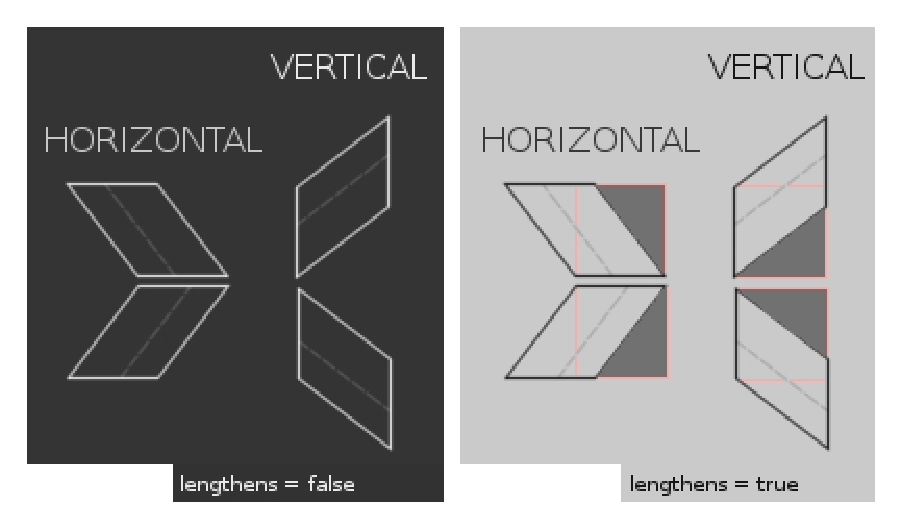
\includegraphics[width=\textwidth,height=\textheight/2,keepaspectratio=true]{images/distort_example}}
\end{DoxyImageNoCaption}



\begin{DoxyParams}{Parameters}
{\em image} & Image to slant \\
\hline
{\em x0} & Start x coordinate of followed line \\
\hline
{\em y0} & Start y coordinate of followed line \\
\hline
{\em x1} & End x coordinate of followed line \\
\hline
{\em y1} & End y coordinate of followed line \\
\hline
{\em orientation} & Vertical or Horizontal slant \\
\hline
{\em lengthens} & If T\+R\+UE the pixels that are \textquotesingle{}empty\textquotesingle{} after the operation will be setted with the value of the last pixel in that line, else if F\+A\+L\+SE that pixels will be setted with total transparency and base color black. \\
\hline
\end{DoxyParams}
\begin{DoxyReturn}{Returns}
Result image
\end{DoxyReturn}
\begin{DoxySeeAlso}{See also}
\hyperlink{header_8h_aef27fcac7a96d118b3c3194c2577049f}{Imel\+Orientation} 

\hyperlink{image_8c_a66997f20203b384d1185a1dd9985dd67}{imel\+\_\+image\+\_\+shift} 

\hyperlink{image_8c_add471c449ecce1b4bd78fc34a698f44f}{imel\+\_\+image\+\_\+shift\+\_\+lines} 

\hyperlink{image_8c_ad08c629d2c44d24e7c485b7ff9a28021}{imel\+\_\+image\+\_\+perspective} 
\end{DoxySeeAlso}
\index{image.\+c@{image.\+c}!imel\+\_\+image\+\_\+union@{imel\+\_\+image\+\_\+union}}
\index{imel\+\_\+image\+\_\+union@{imel\+\_\+image\+\_\+union}!image.\+c@{image.\+c}}
\subsubsection[{\texorpdfstring{imel\+\_\+image\+\_\+union(\+Imel\+Image $\ast$img1, Imel\+Image $\ast$img2, unsigned char opacity, Imel\+Alignment alignment)}{imel_image_union(ImelImage *img1, ImelImage *img2, unsigned char opacity, ImelAlignment alignment)}}]{\setlength{\rightskip}{0pt plus 5cm}{\bf Imel\+Image}$\ast$ imel\+\_\+image\+\_\+union (
\begin{DoxyParamCaption}
\item[{{\bf Imel\+Image} $\ast$}]{img1, }
\item[{{\bf Imel\+Image} $\ast$}]{img2, }
\item[{unsigned char}]{opacity, }
\item[{{\bf Imel\+Alignment}}]{alignment}
\end{DoxyParamCaption}
)}\hypertarget{image_8c_a12519cad063897a1dcf9eb4c677b8304}{}\label{image_8c_a12519cad063897a1dcf9eb4c677b8304}


Insert an image in another with a chosen opacity. 

This function insert {\ttfamily img2} over {\ttfamily img1} with a chosen {\ttfamily opacity} at position specified by {\ttfamily alignment}.


\begin{DoxyParams}{Parameters}
{\em img1} & Base image \\
\hline
{\em img2} & Image to insert over {\ttfamily img1} \\
\hline
{\em opacity} & Opacity of {\ttfamily img2}. Values between 0 and 255. \\
\hline
{\em alignment} & Alignment of {\ttfamily img2} in {\ttfamily img1} \\
\hline
\end{DoxyParams}
\begin{DoxyReturn}{Returns}
Result image
\end{DoxyReturn}
\begin{DoxySeeAlso}{See also}
\hyperlink{pixel_8c_acafccb8e6ccf0cb329498d8343ba1775}{imel\+\_\+pixel\+\_\+union} 

\hyperlink{header_8h_a4d620b3c547205ca76d92f43f09320d1}{Imel\+Alignment} 
\end{DoxySeeAlso}

\hypertarget{image__enum_8h}{}\section{image\+\_\+enum.\+h File Reference}
\label{image__enum_8h}\index{image\+\_\+enum.\+h@{image\+\_\+enum.\+h}}


This file contains enums with options when open and save image file.  


This graph shows which files directly or indirectly include this file\+:
\nopagebreak
\begin{figure}[H]
\begin{center}
\leavevmode
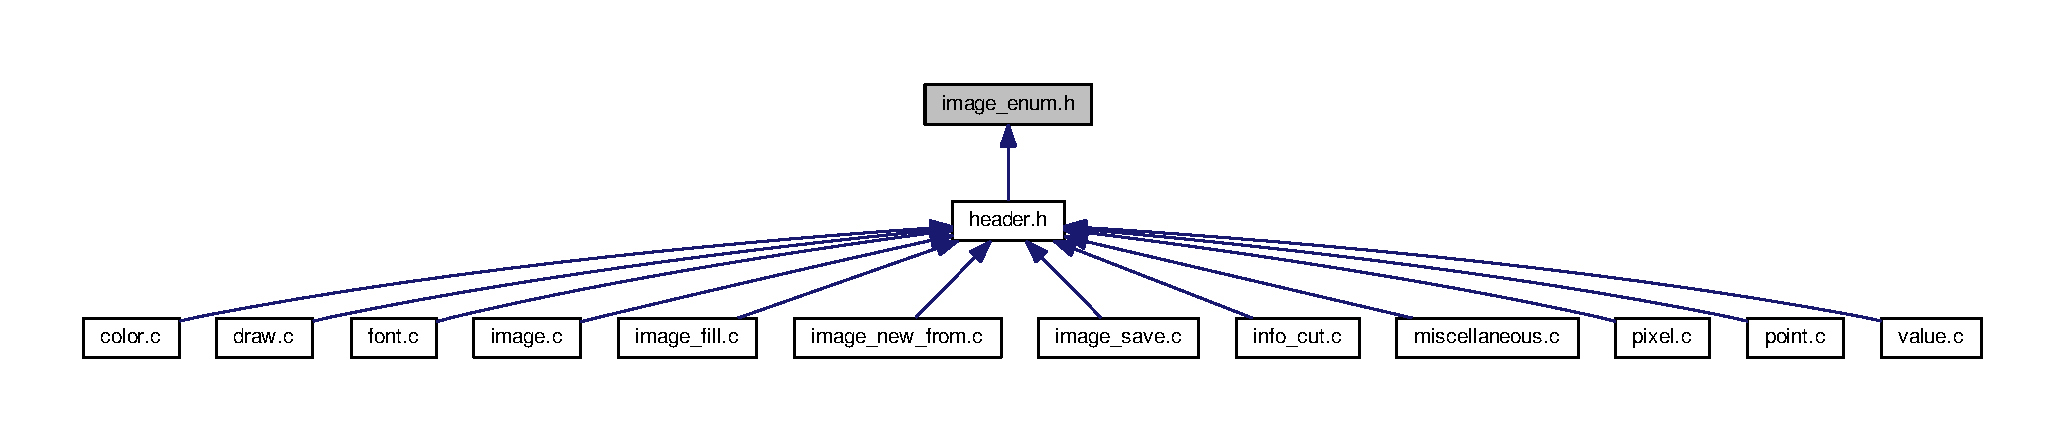
\includegraphics[width=350pt]{image__enum_8h__dep__incl}
\end{center}
\end{figure}
\subsection*{Typedefs}
\begin{DoxyCompactItemize}
\item 
typedef enum \hyperlink{image__enum_8h_ada13fe289edd963e64b938093ef46bd8}{\+\_\+imel\+\_\+jpeg\+\_\+load\+\_\+flags} \hyperlink{image__enum_8h_a26855928d18f44de0b410c4e481215d0}{Imel\+Jpeg\+Load\+Flags}
\item 
typedef enum \hyperlink{image__enum_8h_a59ebb3ac2e672559167fc50d88a70b9c}{\+\_\+imel\+\_\+png\+\_\+load\+\_\+flags} \hyperlink{image__enum_8h_a9b61323ba1a40fa051e89e4f09d4cd12}{Imel\+Png\+Load\+Flags}
\item 
typedef enum \hyperlink{image__enum_8h_aeed3f81cbb1fb964b622aa2e7e0d6c02}{\+\_\+imel\+\_\+tiff\+\_\+load\+\_\+flags} \hyperlink{image__enum_8h_a6a075ca8fec1ae793bf2806e6dccc63a}{Imel\+Tiff\+Load\+Flags}
\item 
typedef enum \hyperlink{image__enum_8h_a31345c3c9d479f29377e84463e9812d0}{\+\_\+imel\+\_\+ico\+\_\+load\+\_\+flags} \hyperlink{image__enum_8h_a1b7f0ec545f50399e90551dd4bf28a0f}{Imel\+Ico\+Load\+Flags}
\item 
typedef enum \hyperlink{image__enum_8h_a7ef186f66edba601bd5da063a9adfb2e}{\+\_\+imel\+\_\+pcd\+\_\+load\+\_\+flags} \hyperlink{image__enum_8h_ac95da0b3430c3995dd2120274a8330e6}{Imel\+Pcd\+Load\+Flags}
\item 
typedef enum \hyperlink{image__enum_8h_a452f46a8e3310e9a42ced6ffb3d5b42e}{\+\_\+imel\+\_\+gif\+\_\+load\+\_\+flags} \hyperlink{image__enum_8h_a560fc8653a85af5ac870cbb46f4c4c9f}{Imel\+Gif\+Load\+Flags}
\item 
typedef enum \hyperlink{image__enum_8h_a24261a698b1c81fa3bc92efb47b9001c}{\+\_\+imel\+\_\+tiff\+\_\+flags} \hyperlink{image__enum_8h_a519baf325b02bcca1d7eab10604c3a75}{Imel\+Tiff\+Flags}
\item 
typedef enum \hyperlink{image__enum_8h_afaf6de3d2895743dc474b3d0528acc90}{\+\_\+imel\+\_\+png\+\_\+flags} \hyperlink{image__enum_8h_a99c2986d48a651287d92e1f419f16a70}{Imel\+Png\+Flags}
\item 
typedef enum \hyperlink{image__enum_8h_a93ede7fe262d0bb3a82340a957096991}{\+\_\+imel\+\_\+bmp\+\_\+bits} \hyperlink{image__enum_8h_acb527c56bb1574fab526fc3a56bf6467}{Imel\+Bmp\+Bits}
\item 
typedef enum \hyperlink{image__enum_8h_a4d02ad7a9a97b77d19ac973dc5b2b039}{\+\_\+imel\+\_\+j2k\+\_\+bits} \hyperlink{image__enum_8h_a75c4f86d6bd9c093d99f5816f84da19d}{Imel\+J2k\+Bits}
\end{DoxyCompactItemize}
\subsection*{Enumerations}


\subsection{Detailed Description}
This file contains enums with options when open and save image file. 

\begin{DoxyAuthor}{Author}
Davide Francesco Merico 
\end{DoxyAuthor}


\subsection{Typedef Documentation}
\index{image\+\_\+enum.\+h@{image\+\_\+enum.\+h}!Imel\+Bmp\+Bits@{Imel\+Bmp\+Bits}}
\index{Imel\+Bmp\+Bits@{Imel\+Bmp\+Bits}!image\+\_\+enum.\+h@{image\+\_\+enum.\+h}}
\subsubsection[{\texorpdfstring{Imel\+Bmp\+Bits}{ImelBmpBits}}]{\setlength{\rightskip}{0pt plus 5cm}typedef enum {\bf \+\_\+imel\+\_\+bmp\+\_\+bits}  {\bf Imel\+Bmp\+Bits}}\hypertarget{image__enum_8h_acb527c56bb1574fab526fc3a56bf6467}{}\label{image__enum_8h_acb527c56bb1574fab526fc3a56bf6467}
Options when saves B\+MP images.

\begin{DoxySeeAlso}{See also}
\hyperlink{image__save_8c_a49c937b0bf49cbe0d16b1d99895a5a2c}{imel\+\_\+image\+\_\+save\+\_\+bmp} 

\hyperlink{image__save_8c_a5c16cf3bd82cedc0ef11698a138f48a2}{imel\+\_\+image\+\_\+save\+\_\+bmp\+\_\+handle} 
\end{DoxySeeAlso}
\index{image\+\_\+enum.\+h@{image\+\_\+enum.\+h}!Imel\+Gif\+Load\+Flags@{Imel\+Gif\+Load\+Flags}}
\index{Imel\+Gif\+Load\+Flags@{Imel\+Gif\+Load\+Flags}!image\+\_\+enum.\+h@{image\+\_\+enum.\+h}}
\subsubsection[{\texorpdfstring{Imel\+Gif\+Load\+Flags}{ImelGifLoadFlags}}]{\setlength{\rightskip}{0pt plus 5cm}typedef enum {\bf \+\_\+imel\+\_\+gif\+\_\+load\+\_\+flags}  {\bf Imel\+Gif\+Load\+Flags}}\hypertarget{image__enum_8h_a560fc8653a85af5ac870cbb46f4c4c9f}{}\label{image__enum_8h_a560fc8653a85af5ac870cbb46f4c4c9f}
Options when opens G\+IF images

\begin{DoxySeeAlso}{See also}
\hyperlink{image__new__from_8c_ade94cb72238022676159bc0f02faf317}{imel\+\_\+image\+\_\+new\+\_\+from\+\_\+gif} 

\hyperlink{image__new__from_8c_a23da123c043b39f035ddd023de022fd0}{imel\+\_\+image\+\_\+new\+\_\+from\+\_\+gif\+\_\+handle} 

\hyperlink{image__new__from_8c_adae15f11a70c3d48541fbfe98547ac8b}{imel\+\_\+image\+\_\+new\+\_\+from\+\_\+gif\+\_\+memory} 
\end{DoxySeeAlso}
\index{image\+\_\+enum.\+h@{image\+\_\+enum.\+h}!Imel\+Ico\+Load\+Flags@{Imel\+Ico\+Load\+Flags}}
\index{Imel\+Ico\+Load\+Flags@{Imel\+Ico\+Load\+Flags}!image\+\_\+enum.\+h@{image\+\_\+enum.\+h}}
\subsubsection[{\texorpdfstring{Imel\+Ico\+Load\+Flags}{ImelIcoLoadFlags}}]{\setlength{\rightskip}{0pt plus 5cm}typedef enum {\bf \+\_\+imel\+\_\+ico\+\_\+load\+\_\+flags}  {\bf Imel\+Ico\+Load\+Flags}}\hypertarget{image__enum_8h_a1b7f0ec545f50399e90551dd4bf28a0f}{}\label{image__enum_8h_a1b7f0ec545f50399e90551dd4bf28a0f}
Options when opens I\+CO images.

\begin{DoxySeeAlso}{See also}
\hyperlink{image__new__from_8c_ad07ca24e2f651581a93b7d5b724d15dd}{imel\+\_\+image\+\_\+new\+\_\+from\+\_\+ico} 

\hyperlink{image__new__from_8c_ab283e173acf0256cb68e7a90bc2108ea}{imel\+\_\+image\+\_\+new\+\_\+from\+\_\+ico\+\_\+handle} 

\hyperlink{image__new__from_8c_a66fd321e9a42de7d2b0dd4f2394691e4}{imel\+\_\+image\+\_\+new\+\_\+from\+\_\+ico\+\_\+memory} 
\end{DoxySeeAlso}
\index{image\+\_\+enum.\+h@{image\+\_\+enum.\+h}!Imel\+J2k\+Bits@{Imel\+J2k\+Bits}}
\index{Imel\+J2k\+Bits@{Imel\+J2k\+Bits}!image\+\_\+enum.\+h@{image\+\_\+enum.\+h}}
\subsubsection[{\texorpdfstring{Imel\+J2k\+Bits}{ImelJ2kBits}}]{\setlength{\rightskip}{0pt plus 5cm}typedef enum {\bf \+\_\+imel\+\_\+j2k\+\_\+bits}  {\bf Imel\+J2k\+Bits}}\hypertarget{image__enum_8h_a75c4f86d6bd9c093d99f5816f84da19d}{}\label{image__enum_8h_a75c4f86d6bd9c093d99f5816f84da19d}
Options when saves J2\+K/\+J\+P2 images

\begin{DoxySeeAlso}{See also}
\hyperlink{image__save_8c_a5ae9a290272e18ad24a6ea9b54784048}{imel\+\_\+image\+\_\+save\+\_\+j2k} 

\hyperlink{image__save_8c_afd3d307d7c5df250aa340dc54576ea12}{imel\+\_\+image\+\_\+save\+\_\+j2k\+\_\+handle} 

\hyperlink{image__save_8c_aa1cdfb54662c2df3573cdca6de25ad63}{imel\+\_\+image\+\_\+save\+\_\+jp2} 

\hyperlink{image__save_8c_a70642f0e5d723ba1c46e8b7739d77d14}{imel\+\_\+image\+\_\+save\+\_\+jp2\+\_\+handle} 
\end{DoxySeeAlso}
\index{image\+\_\+enum.\+h@{image\+\_\+enum.\+h}!Imel\+Jpeg\+Load\+Flags@{Imel\+Jpeg\+Load\+Flags}}
\index{Imel\+Jpeg\+Load\+Flags@{Imel\+Jpeg\+Load\+Flags}!image\+\_\+enum.\+h@{image\+\_\+enum.\+h}}
\subsubsection[{\texorpdfstring{Imel\+Jpeg\+Load\+Flags}{ImelJpegLoadFlags}}]{\setlength{\rightskip}{0pt plus 5cm}typedef enum {\bf \+\_\+imel\+\_\+jpeg\+\_\+load\+\_\+flags}  {\bf Imel\+Jpeg\+Load\+Flags}}\hypertarget{image__enum_8h_a26855928d18f44de0b410c4e481215d0}{}\label{image__enum_8h_a26855928d18f44de0b410c4e481215d0}
Options when opens J\+P\+EG images.

\begin{DoxySeeAlso}{See also}
\hyperlink{image__new__from_8c_a0e52940557ae0c41e132db213a70afd4}{imel\+\_\+image\+\_\+new\+\_\+from\+\_\+jpeg} 

\hyperlink{image__new__from_8c_a255854b1e1dc8be8445f666894332145}{imel\+\_\+image\+\_\+new\+\_\+from\+\_\+jpeg\+\_\+handle} 

\hyperlink{image__new__from_8c_a91fe1c254d77bb29cf84d9e12a747727}{imel\+\_\+image\+\_\+new\+\_\+from\+\_\+jpeg\+\_\+memory} 
\end{DoxySeeAlso}
\index{image\+\_\+enum.\+h@{image\+\_\+enum.\+h}!Imel\+Pcd\+Load\+Flags@{Imel\+Pcd\+Load\+Flags}}
\index{Imel\+Pcd\+Load\+Flags@{Imel\+Pcd\+Load\+Flags}!image\+\_\+enum.\+h@{image\+\_\+enum.\+h}}
\subsubsection[{\texorpdfstring{Imel\+Pcd\+Load\+Flags}{ImelPcdLoadFlags}}]{\setlength{\rightskip}{0pt plus 5cm}typedef enum {\bf \+\_\+imel\+\_\+pcd\+\_\+load\+\_\+flags}  {\bf Imel\+Pcd\+Load\+Flags}}\hypertarget{image__enum_8h_ac95da0b3430c3995dd2120274a8330e6}{}\label{image__enum_8h_ac95da0b3430c3995dd2120274a8330e6}
Options when opens P\+CD images

\begin{DoxySeeAlso}{See also}
\hyperlink{image__new__from_8c_acf1ea6052877363a40e68480f57ba3be}{imel\+\_\+image\+\_\+new\+\_\+from\+\_\+pcd} 

\hyperlink{image__new__from_8c_a4234d2c0b1df5f05d77224d1c1c5f06a}{imel\+\_\+image\+\_\+new\+\_\+from\+\_\+pcd\+\_\+handle} 

\hyperlink{image__new__from_8c_a76c5fbf50c026484258ee9ade2089fa2}{imel\+\_\+image\+\_\+new\+\_\+from\+\_\+pcd\+\_\+memory} 
\end{DoxySeeAlso}
\index{image\+\_\+enum.\+h@{image\+\_\+enum.\+h}!Imel\+Png\+Flags@{Imel\+Png\+Flags}}
\index{Imel\+Png\+Flags@{Imel\+Png\+Flags}!image\+\_\+enum.\+h@{image\+\_\+enum.\+h}}
\subsubsection[{\texorpdfstring{Imel\+Png\+Flags}{ImelPngFlags}}]{\setlength{\rightskip}{0pt plus 5cm}typedef enum {\bf \+\_\+imel\+\_\+png\+\_\+flags}  {\bf Imel\+Png\+Flags}}\hypertarget{image__enum_8h_a99c2986d48a651287d92e1f419f16a70}{}\label{image__enum_8h_a99c2986d48a651287d92e1f419f16a70}
Options when saves P\+NG images.

\begin{DoxySeeAlso}{See also}
\hyperlink{image__save_8c_aa3e1e270563781e46013c98d05e952e7}{imel\+\_\+image\+\_\+save\+\_\+png} 

\hyperlink{image__save_8c_a727418390792881b6262e6392c476ba9}{imel\+\_\+image\+\_\+save\+\_\+png\+\_\+handle} 
\end{DoxySeeAlso}
\index{image\+\_\+enum.\+h@{image\+\_\+enum.\+h}!Imel\+Png\+Load\+Flags@{Imel\+Png\+Load\+Flags}}
\index{Imel\+Png\+Load\+Flags@{Imel\+Png\+Load\+Flags}!image\+\_\+enum.\+h@{image\+\_\+enum.\+h}}
\subsubsection[{\texorpdfstring{Imel\+Png\+Load\+Flags}{ImelPngLoadFlags}}]{\setlength{\rightskip}{0pt plus 5cm}typedef enum {\bf \+\_\+imel\+\_\+png\+\_\+load\+\_\+flags}  {\bf Imel\+Png\+Load\+Flags}}\hypertarget{image__enum_8h_a9b61323ba1a40fa051e89e4f09d4cd12}{}\label{image__enum_8h_a9b61323ba1a40fa051e89e4f09d4cd12}
Options when opens P\+NG images.

\begin{DoxySeeAlso}{See also}
\hyperlink{image__new__from_8c_a479e487f5bf0995932ed8a5ec05cd030}{imel\+\_\+image\+\_\+new\+\_\+from\+\_\+png} 

\hyperlink{image__new__from_8c_acf9c896ceea45e10a991780407c3c259}{imel\+\_\+image\+\_\+new\+\_\+from\+\_\+png\+\_\+handle} 

\hyperlink{image__new__from_8c_a834d3fef3f5336c6d294e84afb0f0a62}{imel\+\_\+image\+\_\+new\+\_\+from\+\_\+png\+\_\+memory} 
\end{DoxySeeAlso}
\index{image\+\_\+enum.\+h@{image\+\_\+enum.\+h}!Imel\+Tiff\+Flags@{Imel\+Tiff\+Flags}}
\index{Imel\+Tiff\+Flags@{Imel\+Tiff\+Flags}!image\+\_\+enum.\+h@{image\+\_\+enum.\+h}}
\subsubsection[{\texorpdfstring{Imel\+Tiff\+Flags}{ImelTiffFlags}}]{\setlength{\rightskip}{0pt plus 5cm}typedef enum {\bf \+\_\+imel\+\_\+tiff\+\_\+flags}  {\bf Imel\+Tiff\+Flags}}\hypertarget{image__enum_8h_a519baf325b02bcca1d7eab10604c3a75}{}\label{image__enum_8h_a519baf325b02bcca1d7eab10604c3a75}
Options when saves T\+I\+FF images

\begin{DoxySeeAlso}{See also}
\hyperlink{image__save_8c_afc28c02ce6aa3ae5fe765510603c51be}{imel\+\_\+image\+\_\+save\+\_\+tiff} 

\hyperlink{image__save_8c_a2e41ce825e969c57d1931fb58a05e920}{imel\+\_\+image\+\_\+save\+\_\+tiff\+\_\+handle} 
\end{DoxySeeAlso}
\index{image\+\_\+enum.\+h@{image\+\_\+enum.\+h}!Imel\+Tiff\+Load\+Flags@{Imel\+Tiff\+Load\+Flags}}
\index{Imel\+Tiff\+Load\+Flags@{Imel\+Tiff\+Load\+Flags}!image\+\_\+enum.\+h@{image\+\_\+enum.\+h}}
\subsubsection[{\texorpdfstring{Imel\+Tiff\+Load\+Flags}{ImelTiffLoadFlags}}]{\setlength{\rightskip}{0pt plus 5cm}typedef enum {\bf \+\_\+imel\+\_\+tiff\+\_\+load\+\_\+flags}  {\bf Imel\+Tiff\+Load\+Flags}}\hypertarget{image__enum_8h_a6a075ca8fec1ae793bf2806e6dccc63a}{}\label{image__enum_8h_a6a075ca8fec1ae793bf2806e6dccc63a}
Options when opens T\+I\+FF images.

\begin{DoxySeeAlso}{See also}
\hyperlink{image__new__from_8c_a00fa94d7b7737a3112030ae792479662}{imel\+\_\+image\+\_\+new\+\_\+from\+\_\+tiff} 

\hyperlink{image__new__from_8c_af02f902b678626b6e015209d0dcbb3ba}{imel\+\_\+image\+\_\+new\+\_\+from\+\_\+tiff\+\_\+handle} 

\hyperlink{image__new__from_8c_a6f49e56a0ea5eeb96be3381dd8e6813b}{imel\+\_\+image\+\_\+new\+\_\+from\+\_\+tiff\+\_\+memory} 
\end{DoxySeeAlso}


\subsection{Enumeration Type Documentation}
\index{image\+\_\+enum.\+h@{image\+\_\+enum.\+h}!\+\_\+imel\+\_\+bmp\+\_\+bits@{\+\_\+imel\+\_\+bmp\+\_\+bits}}
\index{\+\_\+imel\+\_\+bmp\+\_\+bits@{\+\_\+imel\+\_\+bmp\+\_\+bits}!image\+\_\+enum.\+h@{image\+\_\+enum.\+h}}
\subsubsection[{\texorpdfstring{\+\_\+imel\+\_\+bmp\+\_\+bits}{_imel_bmp_bits}}]{\setlength{\rightskip}{0pt plus 5cm}enum {\bf \+\_\+imel\+\_\+bmp\+\_\+bits}}\hypertarget{image__enum_8h_a93ede7fe262d0bb3a82340a957096991}{}\label{image__enum_8h_a93ede7fe262d0bb3a82340a957096991}
Options when saves B\+MP images.

\begin{DoxySeeAlso}{See also}
\hyperlink{image__save_8c_a49c937b0bf49cbe0d16b1d99895a5a2c}{imel\+\_\+image\+\_\+save\+\_\+bmp} 

\hyperlink{image__save_8c_a5c16cf3bd82cedc0ef11698a138f48a2}{imel\+\_\+image\+\_\+save\+\_\+bmp\+\_\+handle} 
\end{DoxySeeAlso}
\begin{Desc}
\item[Enumerator]\par
\begin{description}
\index{I\+M\+E\+L\+\_\+\+B\+M\+P\+\_\+\+B\+I\+T\+S\+\_\+24@{I\+M\+E\+L\+\_\+\+B\+M\+P\+\_\+\+B\+I\+T\+S\+\_\+24}!image\+\_\+enum.\+h@{image\+\_\+enum.\+h}}\index{image\+\_\+enum.\+h@{image\+\_\+enum.\+h}!I\+M\+E\+L\+\_\+\+B\+M\+P\+\_\+\+B\+I\+T\+S\+\_\+24@{I\+M\+E\+L\+\_\+\+B\+M\+P\+\_\+\+B\+I\+T\+S\+\_\+24}}\item[{\em 
I\+M\+E\+L\+\_\+\+B\+M\+P\+\_\+\+B\+I\+T\+S\+\_\+24\hypertarget{image__enum_8h_a93ede7fe262d0bb3a82340a957096991aa7d4d7dd6e59b0b43df10c6e06db2327}{}\label{image__enum_8h_a93ede7fe262d0bb3a82340a957096991aa7d4d7dd6e59b0b43df10c6e06db2327}
}]Saves the B\+MP image with no alpha \index{I\+M\+E\+L\+\_\+\+B\+M\+P\+\_\+\+B\+I\+T\+S\+\_\+32@{I\+M\+E\+L\+\_\+\+B\+M\+P\+\_\+\+B\+I\+T\+S\+\_\+32}!image\+\_\+enum.\+h@{image\+\_\+enum.\+h}}\index{image\+\_\+enum.\+h@{image\+\_\+enum.\+h}!I\+M\+E\+L\+\_\+\+B\+M\+P\+\_\+\+B\+I\+T\+S\+\_\+32@{I\+M\+E\+L\+\_\+\+B\+M\+P\+\_\+\+B\+I\+T\+S\+\_\+32}}\item[{\em 
I\+M\+E\+L\+\_\+\+B\+M\+P\+\_\+\+B\+I\+T\+S\+\_\+32\hypertarget{image__enum_8h_a93ede7fe262d0bb3a82340a957096991a3ef0e6ec175515a2ffe71ee40855e475}{}\label{image__enum_8h_a93ede7fe262d0bb3a82340a957096991a3ef0e6ec175515a2ffe71ee40855e475}
}]Saves the B\+MP image with alpha \end{description}
\end{Desc}
\index{image\+\_\+enum.\+h@{image\+\_\+enum.\+h}!\+\_\+imel\+\_\+gif\+\_\+load\+\_\+flags@{\+\_\+imel\+\_\+gif\+\_\+load\+\_\+flags}}
\index{\+\_\+imel\+\_\+gif\+\_\+load\+\_\+flags@{\+\_\+imel\+\_\+gif\+\_\+load\+\_\+flags}!image\+\_\+enum.\+h@{image\+\_\+enum.\+h}}
\subsubsection[{\texorpdfstring{\+\_\+imel\+\_\+gif\+\_\+load\+\_\+flags}{_imel_gif_load_flags}}]{\setlength{\rightskip}{0pt plus 5cm}enum {\bf \+\_\+imel\+\_\+gif\+\_\+load\+\_\+flags}}\hypertarget{image__enum_8h_a452f46a8e3310e9a42ced6ffb3d5b42e}{}\label{image__enum_8h_a452f46a8e3310e9a42ced6ffb3d5b42e}
Options when opens G\+IF images

\begin{DoxySeeAlso}{See also}
\hyperlink{image__new__from_8c_ade94cb72238022676159bc0f02faf317}{imel\+\_\+image\+\_\+new\+\_\+from\+\_\+gif} 

\hyperlink{image__new__from_8c_a23da123c043b39f035ddd023de022fd0}{imel\+\_\+image\+\_\+new\+\_\+from\+\_\+gif\+\_\+handle} 

\hyperlink{image__new__from_8c_adae15f11a70c3d48541fbfe98547ac8b}{imel\+\_\+image\+\_\+new\+\_\+from\+\_\+gif\+\_\+memory} 
\end{DoxySeeAlso}
\begin{Desc}
\item[Enumerator]\par
\begin{description}
\index{I\+M\+E\+L\+\_\+\+G\+I\+F\+\_\+\+D\+E\+F\+A\+U\+LT@{I\+M\+E\+L\+\_\+\+G\+I\+F\+\_\+\+D\+E\+F\+A\+U\+LT}!image\+\_\+enum.\+h@{image\+\_\+enum.\+h}}\index{image\+\_\+enum.\+h@{image\+\_\+enum.\+h}!I\+M\+E\+L\+\_\+\+G\+I\+F\+\_\+\+D\+E\+F\+A\+U\+LT@{I\+M\+E\+L\+\_\+\+G\+I\+F\+\_\+\+D\+E\+F\+A\+U\+LT}}\item[{\em 
I\+M\+E\+L\+\_\+\+G\+I\+F\+\_\+\+D\+E\+F\+A\+U\+LT\hypertarget{image__enum_8h_a452f46a8e3310e9a42ced6ffb3d5b42eab965572258739a37340a63fb34b21a00}{}\label{image__enum_8h_a452f46a8e3310e9a42ced6ffb3d5b42eab965572258739a37340a63fb34b21a00}
}]Loads the G\+IF image normally \index{I\+M\+E\+L\+\_\+\+G\+I\+F\+\_\+\+L\+O\+A\+D256@{I\+M\+E\+L\+\_\+\+G\+I\+F\+\_\+\+L\+O\+A\+D256}!image\+\_\+enum.\+h@{image\+\_\+enum.\+h}}\index{image\+\_\+enum.\+h@{image\+\_\+enum.\+h}!I\+M\+E\+L\+\_\+\+G\+I\+F\+\_\+\+L\+O\+A\+D256@{I\+M\+E\+L\+\_\+\+G\+I\+F\+\_\+\+L\+O\+A\+D256}}\item[{\em 
I\+M\+E\+L\+\_\+\+G\+I\+F\+\_\+\+L\+O\+A\+D256\hypertarget{image__enum_8h_a452f46a8e3310e9a42ced6ffb3d5b42eafefa851250a3af17e1950a23356c6495}{}\label{image__enum_8h_a452f46a8e3310e9a42ced6ffb3d5b42eafefa851250a3af17e1950a23356c6495}
}]Loads the G\+IF image with only 256 colors \end{description}
\end{Desc}
\index{image\+\_\+enum.\+h@{image\+\_\+enum.\+h}!\+\_\+imel\+\_\+ico\+\_\+load\+\_\+flags@{\+\_\+imel\+\_\+ico\+\_\+load\+\_\+flags}}
\index{\+\_\+imel\+\_\+ico\+\_\+load\+\_\+flags@{\+\_\+imel\+\_\+ico\+\_\+load\+\_\+flags}!image\+\_\+enum.\+h@{image\+\_\+enum.\+h}}
\subsubsection[{\texorpdfstring{\+\_\+imel\+\_\+ico\+\_\+load\+\_\+flags}{_imel_ico_load_flags}}]{\setlength{\rightskip}{0pt plus 5cm}enum {\bf \+\_\+imel\+\_\+ico\+\_\+load\+\_\+flags}}\hypertarget{image__enum_8h_a31345c3c9d479f29377e84463e9812d0}{}\label{image__enum_8h_a31345c3c9d479f29377e84463e9812d0}
Options when opens I\+CO images.

\begin{DoxySeeAlso}{See also}
\hyperlink{image__new__from_8c_ad07ca24e2f651581a93b7d5b724d15dd}{imel\+\_\+image\+\_\+new\+\_\+from\+\_\+ico} 

\hyperlink{image__new__from_8c_ab283e173acf0256cb68e7a90bc2108ea}{imel\+\_\+image\+\_\+new\+\_\+from\+\_\+ico\+\_\+handle} 

\hyperlink{image__new__from_8c_a66fd321e9a42de7d2b0dd4f2394691e4}{imel\+\_\+image\+\_\+new\+\_\+from\+\_\+ico\+\_\+memory} 
\end{DoxySeeAlso}
\begin{Desc}
\item[Enumerator]\par
\begin{description}
\index{I\+M\+E\+L\+\_\+\+I\+C\+O\+\_\+\+D\+E\+F\+A\+U\+LT@{I\+M\+E\+L\+\_\+\+I\+C\+O\+\_\+\+D\+E\+F\+A\+U\+LT}!image\+\_\+enum.\+h@{image\+\_\+enum.\+h}}\index{image\+\_\+enum.\+h@{image\+\_\+enum.\+h}!I\+M\+E\+L\+\_\+\+I\+C\+O\+\_\+\+D\+E\+F\+A\+U\+LT@{I\+M\+E\+L\+\_\+\+I\+C\+O\+\_\+\+D\+E\+F\+A\+U\+LT}}\item[{\em 
I\+M\+E\+L\+\_\+\+I\+C\+O\+\_\+\+D\+E\+F\+A\+U\+LT\hypertarget{image__enum_8h_a31345c3c9d479f29377e84463e9812d0a464013c14a8664918163e643aa531896}{}\label{image__enum_8h_a31345c3c9d479f29377e84463e9812d0a464013c14a8664918163e643aa531896}
}]Loads the I\+CO image normally \index{I\+M\+E\+L\+\_\+\+I\+C\+O\+\_\+\+M\+A\+K\+E\+A\+L\+P\+HA@{I\+M\+E\+L\+\_\+\+I\+C\+O\+\_\+\+M\+A\+K\+E\+A\+L\+P\+HA}!image\+\_\+enum.\+h@{image\+\_\+enum.\+h}}\index{image\+\_\+enum.\+h@{image\+\_\+enum.\+h}!I\+M\+E\+L\+\_\+\+I\+C\+O\+\_\+\+M\+A\+K\+E\+A\+L\+P\+HA@{I\+M\+E\+L\+\_\+\+I\+C\+O\+\_\+\+M\+A\+K\+E\+A\+L\+P\+HA}}\item[{\em 
I\+M\+E\+L\+\_\+\+I\+C\+O\+\_\+\+M\+A\+K\+E\+A\+L\+P\+HA\hypertarget{image__enum_8h_a31345c3c9d479f29377e84463e9812d0a4377f326dd7ff49f997c4213dca1af37}{}\label{image__enum_8h_a31345c3c9d479f29377e84463e9812d0a4377f326dd7ff49f997c4213dca1af37}
}]Loads the I\+CO image converting it to 32 bit and make an alpha channel from an A\+ND mask while loading. \end{description}
\end{Desc}
\index{image\+\_\+enum.\+h@{image\+\_\+enum.\+h}!\+\_\+imel\+\_\+j2k\+\_\+bits@{\+\_\+imel\+\_\+j2k\+\_\+bits}}
\index{\+\_\+imel\+\_\+j2k\+\_\+bits@{\+\_\+imel\+\_\+j2k\+\_\+bits}!image\+\_\+enum.\+h@{image\+\_\+enum.\+h}}
\subsubsection[{\texorpdfstring{\+\_\+imel\+\_\+j2k\+\_\+bits}{_imel_j2k_bits}}]{\setlength{\rightskip}{0pt plus 5cm}enum {\bf \+\_\+imel\+\_\+j2k\+\_\+bits}}\hypertarget{image__enum_8h_a4d02ad7a9a97b77d19ac973dc5b2b039}{}\label{image__enum_8h_a4d02ad7a9a97b77d19ac973dc5b2b039}
Options when saves J2\+K/\+J\+P2 images

\begin{DoxySeeAlso}{See also}
\hyperlink{image__save_8c_a5ae9a290272e18ad24a6ea9b54784048}{imel\+\_\+image\+\_\+save\+\_\+j2k} 

\hyperlink{image__save_8c_afd3d307d7c5df250aa340dc54576ea12}{imel\+\_\+image\+\_\+save\+\_\+j2k\+\_\+handle} 

\hyperlink{image__save_8c_aa1cdfb54662c2df3573cdca6de25ad63}{imel\+\_\+image\+\_\+save\+\_\+jp2} 

\hyperlink{image__save_8c_a70642f0e5d723ba1c46e8b7739d77d14}{imel\+\_\+image\+\_\+save\+\_\+jp2\+\_\+handle} 
\end{DoxySeeAlso}
\begin{Desc}
\item[Enumerator]\par
\begin{description}
\index{I\+M\+E\+L\+\_\+\+J2\+K\+\_\+\+B\+I\+T\+S\+\_\+24@{I\+M\+E\+L\+\_\+\+J2\+K\+\_\+\+B\+I\+T\+S\+\_\+24}!image\+\_\+enum.\+h@{image\+\_\+enum.\+h}}\index{image\+\_\+enum.\+h@{image\+\_\+enum.\+h}!I\+M\+E\+L\+\_\+\+J2\+K\+\_\+\+B\+I\+T\+S\+\_\+24@{I\+M\+E\+L\+\_\+\+J2\+K\+\_\+\+B\+I\+T\+S\+\_\+24}}\item[{\em 
I\+M\+E\+L\+\_\+\+J2\+K\+\_\+\+B\+I\+T\+S\+\_\+24\hypertarget{image__enum_8h_a4d02ad7a9a97b77d19ac973dc5b2b039a69e00c930ae9e84d58efffbc0c29b33c}{}\label{image__enum_8h_a4d02ad7a9a97b77d19ac973dc5b2b039a69e00c930ae9e84d58efffbc0c29b33c}
}]Saves the J2\+K/\+J\+P2 image with no alpha \index{I\+M\+E\+L\+\_\+\+J2\+K\+\_\+\+B\+I\+T\+S\+\_\+32@{I\+M\+E\+L\+\_\+\+J2\+K\+\_\+\+B\+I\+T\+S\+\_\+32}!image\+\_\+enum.\+h@{image\+\_\+enum.\+h}}\index{image\+\_\+enum.\+h@{image\+\_\+enum.\+h}!I\+M\+E\+L\+\_\+\+J2\+K\+\_\+\+B\+I\+T\+S\+\_\+32@{I\+M\+E\+L\+\_\+\+J2\+K\+\_\+\+B\+I\+T\+S\+\_\+32}}\item[{\em 
I\+M\+E\+L\+\_\+\+J2\+K\+\_\+\+B\+I\+T\+S\+\_\+32\hypertarget{image__enum_8h_a4d02ad7a9a97b77d19ac973dc5b2b039a8bfaf28fbdb042e69f658cdc3f8c6f7d}{}\label{image__enum_8h_a4d02ad7a9a97b77d19ac973dc5b2b039a8bfaf28fbdb042e69f658cdc3f8c6f7d}
}]Saves the J2\+K/\+J\+P2 image with alpha \end{description}
\end{Desc}
\index{image\+\_\+enum.\+h@{image\+\_\+enum.\+h}!\+\_\+imel\+\_\+jpeg\+\_\+load\+\_\+flags@{\+\_\+imel\+\_\+jpeg\+\_\+load\+\_\+flags}}
\index{\+\_\+imel\+\_\+jpeg\+\_\+load\+\_\+flags@{\+\_\+imel\+\_\+jpeg\+\_\+load\+\_\+flags}!image\+\_\+enum.\+h@{image\+\_\+enum.\+h}}
\subsubsection[{\texorpdfstring{\+\_\+imel\+\_\+jpeg\+\_\+load\+\_\+flags}{_imel_jpeg_load_flags}}]{\setlength{\rightskip}{0pt plus 5cm}enum {\bf \+\_\+imel\+\_\+jpeg\+\_\+load\+\_\+flags}}\hypertarget{image__enum_8h_ada13fe289edd963e64b938093ef46bd8}{}\label{image__enum_8h_ada13fe289edd963e64b938093ef46bd8}
Options when opens J\+P\+EG images.

\begin{DoxySeeAlso}{See also}
\hyperlink{image__new__from_8c_a0e52940557ae0c41e132db213a70afd4}{imel\+\_\+image\+\_\+new\+\_\+from\+\_\+jpeg} 

\hyperlink{image__new__from_8c_a255854b1e1dc8be8445f666894332145}{imel\+\_\+image\+\_\+new\+\_\+from\+\_\+jpeg\+\_\+handle} 

\hyperlink{image__new__from_8c_a91fe1c254d77bb29cf84d9e12a747727}{imel\+\_\+image\+\_\+new\+\_\+from\+\_\+jpeg\+\_\+memory} 
\end{DoxySeeAlso}
\begin{Desc}
\item[Enumerator]\par
\begin{description}
\index{I\+M\+E\+L\+\_\+\+J\+P\+E\+G\+\_\+\+D\+E\+F\+A\+U\+LT@{I\+M\+E\+L\+\_\+\+J\+P\+E\+G\+\_\+\+D\+E\+F\+A\+U\+LT}!image\+\_\+enum.\+h@{image\+\_\+enum.\+h}}\index{image\+\_\+enum.\+h@{image\+\_\+enum.\+h}!I\+M\+E\+L\+\_\+\+J\+P\+E\+G\+\_\+\+D\+E\+F\+A\+U\+LT@{I\+M\+E\+L\+\_\+\+J\+P\+E\+G\+\_\+\+D\+E\+F\+A\+U\+LT}}\item[{\em 
I\+M\+E\+L\+\_\+\+J\+P\+E\+G\+\_\+\+D\+E\+F\+A\+U\+LT\hypertarget{image__enum_8h_ada13fe289edd963e64b938093ef46bd8ab66cddd5409899342299e09433766e87}{}\label{image__enum_8h_ada13fe289edd963e64b938093ef46bd8ab66cddd5409899342299e09433766e87}
}]Equal to I\+M\+E\+L\+\_\+\+J\+P\+E\+G\+\_\+\+F\+A\+ST \index{I\+M\+E\+L\+\_\+\+J\+P\+E\+G\+\_\+\+F\+A\+ST@{I\+M\+E\+L\+\_\+\+J\+P\+E\+G\+\_\+\+F\+A\+ST}!image\+\_\+enum.\+h@{image\+\_\+enum.\+h}}\index{image\+\_\+enum.\+h@{image\+\_\+enum.\+h}!I\+M\+E\+L\+\_\+\+J\+P\+E\+G\+\_\+\+F\+A\+ST@{I\+M\+E\+L\+\_\+\+J\+P\+E\+G\+\_\+\+F\+A\+ST}}\item[{\em 
I\+M\+E\+L\+\_\+\+J\+P\+E\+G\+\_\+\+F\+A\+ST\hypertarget{image__enum_8h_ada13fe289edd963e64b938093ef46bd8a8d86e9e55c2e9068fb2bf00686c84dd1}{}\label{image__enum_8h_ada13fe289edd963e64b938093ef46bd8a8d86e9e55c2e9068fb2bf00686c84dd1}
}]Loads the J\+P\+EG image fast but with less quality \index{I\+M\+E\+L\+\_\+\+J\+P\+E\+G\+\_\+\+A\+C\+C\+U\+R\+A\+TE@{I\+M\+E\+L\+\_\+\+J\+P\+E\+G\+\_\+\+A\+C\+C\+U\+R\+A\+TE}!image\+\_\+enum.\+h@{image\+\_\+enum.\+h}}\index{image\+\_\+enum.\+h@{image\+\_\+enum.\+h}!I\+M\+E\+L\+\_\+\+J\+P\+E\+G\+\_\+\+A\+C\+C\+U\+R\+A\+TE@{I\+M\+E\+L\+\_\+\+J\+P\+E\+G\+\_\+\+A\+C\+C\+U\+R\+A\+TE}}\item[{\em 
I\+M\+E\+L\+\_\+\+J\+P\+E\+G\+\_\+\+A\+C\+C\+U\+R\+A\+TE\hypertarget{image__enum_8h_ada13fe289edd963e64b938093ef46bd8af27b86b864d6f248925997539cac52dc}{}\label{image__enum_8h_ada13fe289edd963e64b938093ef46bd8af27b86b864d6f248925997539cac52dc}
}]Loads the J\+P\+EG image with quality but with less velocity \index{I\+M\+E\+L\+\_\+\+J\+P\+E\+G\+\_\+\+C\+M\+YK@{I\+M\+E\+L\+\_\+\+J\+P\+E\+G\+\_\+\+C\+M\+YK}!image\+\_\+enum.\+h@{image\+\_\+enum.\+h}}\index{image\+\_\+enum.\+h@{image\+\_\+enum.\+h}!I\+M\+E\+L\+\_\+\+J\+P\+E\+G\+\_\+\+C\+M\+YK@{I\+M\+E\+L\+\_\+\+J\+P\+E\+G\+\_\+\+C\+M\+YK}}\item[{\em 
I\+M\+E\+L\+\_\+\+J\+P\+E\+G\+\_\+\+C\+M\+YK\hypertarget{image__enum_8h_ada13fe289edd963e64b938093ef46bd8a058f15ba15e339d4b2523649b39abfd9}{}\label{image__enum_8h_ada13fe289edd963e64b938093ef46bd8a058f15ba15e339d4b2523649b39abfd9}
}]Loads the J\+P\+EG image with separed C\+M\+YK channels. \begin{DoxyWarning}{Warning}
Imel convert C\+M\+YK channels to R\+GB channels automatically 
\end{DoxyWarning}
\end{description}
\end{Desc}
\index{image\+\_\+enum.\+h@{image\+\_\+enum.\+h}!\+\_\+imel\+\_\+pcd\+\_\+load\+\_\+flags@{\+\_\+imel\+\_\+pcd\+\_\+load\+\_\+flags}}
\index{\+\_\+imel\+\_\+pcd\+\_\+load\+\_\+flags@{\+\_\+imel\+\_\+pcd\+\_\+load\+\_\+flags}!image\+\_\+enum.\+h@{image\+\_\+enum.\+h}}
\subsubsection[{\texorpdfstring{\+\_\+imel\+\_\+pcd\+\_\+load\+\_\+flags}{_imel_pcd_load_flags}}]{\setlength{\rightskip}{0pt plus 5cm}enum {\bf \+\_\+imel\+\_\+pcd\+\_\+load\+\_\+flags}}\hypertarget{image__enum_8h_a7ef186f66edba601bd5da063a9adfb2e}{}\label{image__enum_8h_a7ef186f66edba601bd5da063a9adfb2e}
Options when opens P\+CD images

\begin{DoxySeeAlso}{See also}
\hyperlink{image__new__from_8c_acf1ea6052877363a40e68480f57ba3be}{imel\+\_\+image\+\_\+new\+\_\+from\+\_\+pcd} 

\hyperlink{image__new__from_8c_a4234d2c0b1df5f05d77224d1c1c5f06a}{imel\+\_\+image\+\_\+new\+\_\+from\+\_\+pcd\+\_\+handle} 

\hyperlink{image__new__from_8c_a76c5fbf50c026484258ee9ade2089fa2}{imel\+\_\+image\+\_\+new\+\_\+from\+\_\+pcd\+\_\+memory} 
\end{DoxySeeAlso}
\begin{Desc}
\item[Enumerator]\par
\begin{description}
\index{I\+M\+E\+L\+\_\+\+P\+C\+D\+\_\+\+D\+E\+F\+A\+U\+LT@{I\+M\+E\+L\+\_\+\+P\+C\+D\+\_\+\+D\+E\+F\+A\+U\+LT}!image\+\_\+enum.\+h@{image\+\_\+enum.\+h}}\index{image\+\_\+enum.\+h@{image\+\_\+enum.\+h}!I\+M\+E\+L\+\_\+\+P\+C\+D\+\_\+\+D\+E\+F\+A\+U\+LT@{I\+M\+E\+L\+\_\+\+P\+C\+D\+\_\+\+D\+E\+F\+A\+U\+LT}}\item[{\em 
I\+M\+E\+L\+\_\+\+P\+C\+D\+\_\+\+D\+E\+F\+A\+U\+LT\hypertarget{image__enum_8h_a7ef186f66edba601bd5da063a9adfb2ea80a9b69f1c4c13936e8b4bfdf2c24d06}{}\label{image__enum_8h_a7ef186f66edba601bd5da063a9adfb2ea80a9b69f1c4c13936e8b4bfdf2c24d06}
}]Equal to I\+M\+E\+L\+\_\+\+P\+C\+D\+\_\+\+B\+A\+SE \index{I\+M\+E\+L\+\_\+\+P\+C\+D\+\_\+\+B\+A\+SE@{I\+M\+E\+L\+\_\+\+P\+C\+D\+\_\+\+B\+A\+SE}!image\+\_\+enum.\+h@{image\+\_\+enum.\+h}}\index{image\+\_\+enum.\+h@{image\+\_\+enum.\+h}!I\+M\+E\+L\+\_\+\+P\+C\+D\+\_\+\+B\+A\+SE@{I\+M\+E\+L\+\_\+\+P\+C\+D\+\_\+\+B\+A\+SE}}\item[{\em 
I\+M\+E\+L\+\_\+\+P\+C\+D\+\_\+\+B\+A\+SE\hypertarget{image__enum_8h_a7ef186f66edba601bd5da063a9adfb2ea2f807222b55260e3d28223dc1c38be57}{}\label{image__enum_8h_a7ef186f66edba601bd5da063a9adfb2ea2f807222b55260e3d28223dc1c38be57}
}]Loads the P\+CD image at resolution of 768x512 pixel \index{I\+M\+E\+L\+\_\+\+P\+C\+D\+\_\+\+B\+A\+S\+E\+D\+I\+V4@{I\+M\+E\+L\+\_\+\+P\+C\+D\+\_\+\+B\+A\+S\+E\+D\+I\+V4}!image\+\_\+enum.\+h@{image\+\_\+enum.\+h}}\index{image\+\_\+enum.\+h@{image\+\_\+enum.\+h}!I\+M\+E\+L\+\_\+\+P\+C\+D\+\_\+\+B\+A\+S\+E\+D\+I\+V4@{I\+M\+E\+L\+\_\+\+P\+C\+D\+\_\+\+B\+A\+S\+E\+D\+I\+V4}}\item[{\em 
I\+M\+E\+L\+\_\+\+P\+C\+D\+\_\+\+B\+A\+S\+E\+D\+I\+V4\hypertarget{image__enum_8h_a7ef186f66edba601bd5da063a9adfb2eaa45d9b8d64c6a5b244373f5e8845b453}{}\label{image__enum_8h_a7ef186f66edba601bd5da063a9adfb2eaa45d9b8d64c6a5b244373f5e8845b453}
}]Loads the P\+CD image at resolution of 384x256 pixel \index{I\+M\+E\+L\+\_\+\+P\+C\+D\+\_\+\+B\+A\+S\+E\+D\+I\+V16@{I\+M\+E\+L\+\_\+\+P\+C\+D\+\_\+\+B\+A\+S\+E\+D\+I\+V16}!image\+\_\+enum.\+h@{image\+\_\+enum.\+h}}\index{image\+\_\+enum.\+h@{image\+\_\+enum.\+h}!I\+M\+E\+L\+\_\+\+P\+C\+D\+\_\+\+B\+A\+S\+E\+D\+I\+V16@{I\+M\+E\+L\+\_\+\+P\+C\+D\+\_\+\+B\+A\+S\+E\+D\+I\+V16}}\item[{\em 
I\+M\+E\+L\+\_\+\+P\+C\+D\+\_\+\+B\+A\+S\+E\+D\+I\+V16\hypertarget{image__enum_8h_a7ef186f66edba601bd5da063a9adfb2ea0ada7359fcbd68b79a106c212f5b2a81}{}\label{image__enum_8h_a7ef186f66edba601bd5da063a9adfb2ea0ada7359fcbd68b79a106c212f5b2a81}
}]Loads the P\+CD image at resolution of 192x128 pixel \end{description}
\end{Desc}
\index{image\+\_\+enum.\+h@{image\+\_\+enum.\+h}!\+\_\+imel\+\_\+png\+\_\+flags@{\+\_\+imel\+\_\+png\+\_\+flags}}
\index{\+\_\+imel\+\_\+png\+\_\+flags@{\+\_\+imel\+\_\+png\+\_\+flags}!image\+\_\+enum.\+h@{image\+\_\+enum.\+h}}
\subsubsection[{\texorpdfstring{\+\_\+imel\+\_\+png\+\_\+flags}{_imel_png_flags}}]{\setlength{\rightskip}{0pt plus 5cm}enum {\bf \+\_\+imel\+\_\+png\+\_\+flags}}\hypertarget{image__enum_8h_afaf6de3d2895743dc474b3d0528acc90}{}\label{image__enum_8h_afaf6de3d2895743dc474b3d0528acc90}
Options when saves P\+NG images.

\begin{DoxySeeAlso}{See also}
\hyperlink{image__save_8c_aa3e1e270563781e46013c98d05e952e7}{imel\+\_\+image\+\_\+save\+\_\+png} 

\hyperlink{image__save_8c_a727418390792881b6262e6392c476ba9}{imel\+\_\+image\+\_\+save\+\_\+png\+\_\+handle} 
\end{DoxySeeAlso}
\begin{Desc}
\item[Enumerator]\par
\begin{description}
\index{I\+M\+E\+L\+\_\+\+P\+N\+G\+\_\+\+Z\+\_\+\+B\+E\+S\+T\+\_\+\+S\+P\+E\+ED@{I\+M\+E\+L\+\_\+\+P\+N\+G\+\_\+\+Z\+\_\+\+B\+E\+S\+T\+\_\+\+S\+P\+E\+ED}!image\+\_\+enum.\+h@{image\+\_\+enum.\+h}}\index{image\+\_\+enum.\+h@{image\+\_\+enum.\+h}!I\+M\+E\+L\+\_\+\+P\+N\+G\+\_\+\+Z\+\_\+\+B\+E\+S\+T\+\_\+\+S\+P\+E\+ED@{I\+M\+E\+L\+\_\+\+P\+N\+G\+\_\+\+Z\+\_\+\+B\+E\+S\+T\+\_\+\+S\+P\+E\+ED}}\item[{\em 
I\+M\+E\+L\+\_\+\+P\+N\+G\+\_\+\+Z\+\_\+\+B\+E\+S\+T\+\_\+\+S\+P\+E\+ED\hypertarget{image__enum_8h_afaf6de3d2895743dc474b3d0528acc90a6ef9b96a3aa221e784baaa63ffd63247}{}\label{image__enum_8h_afaf6de3d2895743dc474b3d0528acc90a6ef9b96a3aa221e784baaa63ffd63247}
}]Saves the P\+NG image using Zlib library with compression value of 1 \index{I\+M\+E\+L\+\_\+\+P\+N\+G\+\_\+\+Z\+\_\+\+D\+E\+F\+A\+U\+L\+T\+\_\+\+C\+O\+M\+P\+R\+E\+S\+S\+I\+ON@{I\+M\+E\+L\+\_\+\+P\+N\+G\+\_\+\+Z\+\_\+\+D\+E\+F\+A\+U\+L\+T\+\_\+\+C\+O\+M\+P\+R\+E\+S\+S\+I\+ON}!image\+\_\+enum.\+h@{image\+\_\+enum.\+h}}\index{image\+\_\+enum.\+h@{image\+\_\+enum.\+h}!I\+M\+E\+L\+\_\+\+P\+N\+G\+\_\+\+Z\+\_\+\+D\+E\+F\+A\+U\+L\+T\+\_\+\+C\+O\+M\+P\+R\+E\+S\+S\+I\+ON@{I\+M\+E\+L\+\_\+\+P\+N\+G\+\_\+\+Z\+\_\+\+D\+E\+F\+A\+U\+L\+T\+\_\+\+C\+O\+M\+P\+R\+E\+S\+S\+I\+ON}}\item[{\em 
I\+M\+E\+L\+\_\+\+P\+N\+G\+\_\+\+Z\+\_\+\+D\+E\+F\+A\+U\+L\+T\+\_\+\+C\+O\+M\+P\+R\+E\+S\+S\+I\+ON\hypertarget{image__enum_8h_afaf6de3d2895743dc474b3d0528acc90a63aa12bbfac02a6f8074be92bc0bbea1}{}\label{image__enum_8h_afaf6de3d2895743dc474b3d0528acc90a63aa12bbfac02a6f8074be92bc0bbea1}
}]Saves the P\+NG image using Zlib library with compression value of 6 \index{I\+M\+E\+L\+\_\+\+P\+N\+G\+\_\+\+Z\+\_\+\+B\+E\+S\+T\+\_\+\+C\+O\+M\+P\+R\+E\+S\+S\+I\+ON@{I\+M\+E\+L\+\_\+\+P\+N\+G\+\_\+\+Z\+\_\+\+B\+E\+S\+T\+\_\+\+C\+O\+M\+P\+R\+E\+S\+S\+I\+ON}!image\+\_\+enum.\+h@{image\+\_\+enum.\+h}}\index{image\+\_\+enum.\+h@{image\+\_\+enum.\+h}!I\+M\+E\+L\+\_\+\+P\+N\+G\+\_\+\+Z\+\_\+\+B\+E\+S\+T\+\_\+\+C\+O\+M\+P\+R\+E\+S\+S\+I\+ON@{I\+M\+E\+L\+\_\+\+P\+N\+G\+\_\+\+Z\+\_\+\+B\+E\+S\+T\+\_\+\+C\+O\+M\+P\+R\+E\+S\+S\+I\+ON}}\item[{\em 
I\+M\+E\+L\+\_\+\+P\+N\+G\+\_\+\+Z\+\_\+\+B\+E\+S\+T\+\_\+\+C\+O\+M\+P\+R\+E\+S\+S\+I\+ON\hypertarget{image__enum_8h_afaf6de3d2895743dc474b3d0528acc90adf009186e35d88163320a337dbc873a1}{}\label{image__enum_8h_afaf6de3d2895743dc474b3d0528acc90adf009186e35d88163320a337dbc873a1}
}]Saves the P\+NG image using Zlib library with compression value of 9 \index{I\+M\+E\+L\+\_\+\+P\+N\+G\+\_\+\+Z\+\_\+\+N\+O\+\_\+\+C\+O\+M\+P\+R\+E\+S\+S\+I\+ON@{I\+M\+E\+L\+\_\+\+P\+N\+G\+\_\+\+Z\+\_\+\+N\+O\+\_\+\+C\+O\+M\+P\+R\+E\+S\+S\+I\+ON}!image\+\_\+enum.\+h@{image\+\_\+enum.\+h}}\index{image\+\_\+enum.\+h@{image\+\_\+enum.\+h}!I\+M\+E\+L\+\_\+\+P\+N\+G\+\_\+\+Z\+\_\+\+N\+O\+\_\+\+C\+O\+M\+P\+R\+E\+S\+S\+I\+ON@{I\+M\+E\+L\+\_\+\+P\+N\+G\+\_\+\+Z\+\_\+\+N\+O\+\_\+\+C\+O\+M\+P\+R\+E\+S\+S\+I\+ON}}\item[{\em 
I\+M\+E\+L\+\_\+\+P\+N\+G\+\_\+\+Z\+\_\+\+N\+O\+\_\+\+C\+O\+M\+P\+R\+E\+S\+S\+I\+ON\hypertarget{image__enum_8h_afaf6de3d2895743dc474b3d0528acc90afae8ce03ab6b9c93b27b7f7fdc0f422a}{}\label{image__enum_8h_afaf6de3d2895743dc474b3d0528acc90afae8ce03ab6b9c93b27b7f7fdc0f422a}
}]Saves the P\+NG image using Zlib library with no compression \index{I\+M\+E\+L\+\_\+\+P\+N\+G\+\_\+\+I\+N\+T\+E\+R\+L\+A\+C\+ED@{I\+M\+E\+L\+\_\+\+P\+N\+G\+\_\+\+I\+N\+T\+E\+R\+L\+A\+C\+ED}!image\+\_\+enum.\+h@{image\+\_\+enum.\+h}}\index{image\+\_\+enum.\+h@{image\+\_\+enum.\+h}!I\+M\+E\+L\+\_\+\+P\+N\+G\+\_\+\+I\+N\+T\+E\+R\+L\+A\+C\+ED@{I\+M\+E\+L\+\_\+\+P\+N\+G\+\_\+\+I\+N\+T\+E\+R\+L\+A\+C\+ED}}\item[{\em 
I\+M\+E\+L\+\_\+\+P\+N\+G\+\_\+\+I\+N\+T\+E\+R\+L\+A\+C\+ED\hypertarget{image__enum_8h_afaf6de3d2895743dc474b3d0528acc90ab8e6f3ce5123cff3b7f0b30201e8f426}{}\label{image__enum_8h_afaf6de3d2895743dc474b3d0528acc90ab8e6f3ce5123cff3b7f0b30201e8f426}
}]Saves the P\+NG image with Adam7 interlacing \end{description}
\end{Desc}
\index{image\+\_\+enum.\+h@{image\+\_\+enum.\+h}!\+\_\+imel\+\_\+png\+\_\+load\+\_\+flags@{\+\_\+imel\+\_\+png\+\_\+load\+\_\+flags}}
\index{\+\_\+imel\+\_\+png\+\_\+load\+\_\+flags@{\+\_\+imel\+\_\+png\+\_\+load\+\_\+flags}!image\+\_\+enum.\+h@{image\+\_\+enum.\+h}}
\subsubsection[{\texorpdfstring{\+\_\+imel\+\_\+png\+\_\+load\+\_\+flags}{_imel_png_load_flags}}]{\setlength{\rightskip}{0pt plus 5cm}enum {\bf \+\_\+imel\+\_\+png\+\_\+load\+\_\+flags}}\hypertarget{image__enum_8h_a59ebb3ac2e672559167fc50d88a70b9c}{}\label{image__enum_8h_a59ebb3ac2e672559167fc50d88a70b9c}
Options when opens P\+NG images.

\begin{DoxySeeAlso}{See also}
\hyperlink{image__new__from_8c_a479e487f5bf0995932ed8a5ec05cd030}{imel\+\_\+image\+\_\+new\+\_\+from\+\_\+png} 

\hyperlink{image__new__from_8c_acf9c896ceea45e10a991780407c3c259}{imel\+\_\+image\+\_\+new\+\_\+from\+\_\+png\+\_\+handle} 

\hyperlink{image__new__from_8c_a834d3fef3f5336c6d294e84afb0f0a62}{imel\+\_\+image\+\_\+new\+\_\+from\+\_\+png\+\_\+memory} 
\end{DoxySeeAlso}
\begin{Desc}
\item[Enumerator]\par
\begin{description}
\index{I\+M\+E\+L\+\_\+\+P\+N\+G\+\_\+\+D\+E\+F\+A\+U\+LT@{I\+M\+E\+L\+\_\+\+P\+N\+G\+\_\+\+D\+E\+F\+A\+U\+LT}!image\+\_\+enum.\+h@{image\+\_\+enum.\+h}}\index{image\+\_\+enum.\+h@{image\+\_\+enum.\+h}!I\+M\+E\+L\+\_\+\+P\+N\+G\+\_\+\+D\+E\+F\+A\+U\+LT@{I\+M\+E\+L\+\_\+\+P\+N\+G\+\_\+\+D\+E\+F\+A\+U\+LT}}\item[{\em 
I\+M\+E\+L\+\_\+\+P\+N\+G\+\_\+\+D\+E\+F\+A\+U\+LT\hypertarget{image__enum_8h_a59ebb3ac2e672559167fc50d88a70b9ca0c9d9cf201358659d38cbb5af3e07d99}{}\label{image__enum_8h_a59ebb3ac2e672559167fc50d88a70b9ca0c9d9cf201358659d38cbb5af3e07d99}
}]Loads the P\+NG image normally \index{I\+M\+E\+L\+\_\+\+P\+N\+G\+\_\+\+I\+G\+N\+O\+R\+E\+G\+A\+M\+MA@{I\+M\+E\+L\+\_\+\+P\+N\+G\+\_\+\+I\+G\+N\+O\+R\+E\+G\+A\+M\+MA}!image\+\_\+enum.\+h@{image\+\_\+enum.\+h}}\index{image\+\_\+enum.\+h@{image\+\_\+enum.\+h}!I\+M\+E\+L\+\_\+\+P\+N\+G\+\_\+\+I\+G\+N\+O\+R\+E\+G\+A\+M\+MA@{I\+M\+E\+L\+\_\+\+P\+N\+G\+\_\+\+I\+G\+N\+O\+R\+E\+G\+A\+M\+MA}}\item[{\em 
I\+M\+E\+L\+\_\+\+P\+N\+G\+\_\+\+I\+G\+N\+O\+R\+E\+G\+A\+M\+MA\hypertarget{image__enum_8h_a59ebb3ac2e672559167fc50d88a70b9caf76f56a95d4b3d4dbf884202ce679335}{}\label{image__enum_8h_a59ebb3ac2e672559167fc50d88a70b9caf76f56a95d4b3d4dbf884202ce679335}
}]Loads the P\+NG image withour gamma correction \end{description}
\end{Desc}
\index{image\+\_\+enum.\+h@{image\+\_\+enum.\+h}!\+\_\+imel\+\_\+tiff\+\_\+flags@{\+\_\+imel\+\_\+tiff\+\_\+flags}}
\index{\+\_\+imel\+\_\+tiff\+\_\+flags@{\+\_\+imel\+\_\+tiff\+\_\+flags}!image\+\_\+enum.\+h@{image\+\_\+enum.\+h}}
\subsubsection[{\texorpdfstring{\+\_\+imel\+\_\+tiff\+\_\+flags}{_imel_tiff_flags}}]{\setlength{\rightskip}{0pt plus 5cm}enum {\bf \+\_\+imel\+\_\+tiff\+\_\+flags}}\hypertarget{image__enum_8h_a24261a698b1c81fa3bc92efb47b9001c}{}\label{image__enum_8h_a24261a698b1c81fa3bc92efb47b9001c}
Options when saves T\+I\+FF images

\begin{DoxySeeAlso}{See also}
\hyperlink{image__save_8c_afc28c02ce6aa3ae5fe765510603c51be}{imel\+\_\+image\+\_\+save\+\_\+tiff} 

\hyperlink{image__save_8c_a2e41ce825e969c57d1931fb58a05e920}{imel\+\_\+image\+\_\+save\+\_\+tiff\+\_\+handle} 
\end{DoxySeeAlso}
\begin{Desc}
\item[Enumerator]\par
\begin{description}
\index{I\+M\+E\+L\+\_\+\+T\+I\+F\+F\+\_\+\+P\+A\+C\+K\+B\+I\+TS@{I\+M\+E\+L\+\_\+\+T\+I\+F\+F\+\_\+\+P\+A\+C\+K\+B\+I\+TS}!image\+\_\+enum.\+h@{image\+\_\+enum.\+h}}\index{image\+\_\+enum.\+h@{image\+\_\+enum.\+h}!I\+M\+E\+L\+\_\+\+T\+I\+F\+F\+\_\+\+P\+A\+C\+K\+B\+I\+TS@{I\+M\+E\+L\+\_\+\+T\+I\+F\+F\+\_\+\+P\+A\+C\+K\+B\+I\+TS}}\item[{\em 
I\+M\+E\+L\+\_\+\+T\+I\+F\+F\+\_\+\+P\+A\+C\+K\+B\+I\+TS\hypertarget{image__enum_8h_a24261a698b1c81fa3bc92efb47b9001ca6c742ee31bba8c22a7b9cf1b7347ce53}{}\label{image__enum_8h_a24261a698b1c81fa3bc92efb47b9001ca6c742ee31bba8c22a7b9cf1b7347ce53}
}]Saves the T\+I\+FF image using P\+A\+C\+K\+B\+I\+TS compression \index{I\+M\+E\+L\+\_\+\+T\+I\+F\+F\+\_\+\+D\+E\+F\+L\+A\+TE@{I\+M\+E\+L\+\_\+\+T\+I\+F\+F\+\_\+\+D\+E\+F\+L\+A\+TE}!image\+\_\+enum.\+h@{image\+\_\+enum.\+h}}\index{image\+\_\+enum.\+h@{image\+\_\+enum.\+h}!I\+M\+E\+L\+\_\+\+T\+I\+F\+F\+\_\+\+D\+E\+F\+L\+A\+TE@{I\+M\+E\+L\+\_\+\+T\+I\+F\+F\+\_\+\+D\+E\+F\+L\+A\+TE}}\item[{\em 
I\+M\+E\+L\+\_\+\+T\+I\+F\+F\+\_\+\+D\+E\+F\+L\+A\+TE\hypertarget{image__enum_8h_a24261a698b1c81fa3bc92efb47b9001ca1b3c10761d8cefa9740ef2987a63b474}{}\label{image__enum_8h_a24261a698b1c81fa3bc92efb47b9001ca1b3c10761d8cefa9740ef2987a63b474}
}]Saves the T\+I\+FF image using D\+E\+F\+L\+A\+TE compression ( Zlib ) \index{I\+M\+E\+L\+\_\+\+T\+I\+F\+F\+\_\+\+A\+D\+O\+B\+E\+\_\+\+D\+E\+F\+L\+A\+TE@{I\+M\+E\+L\+\_\+\+T\+I\+F\+F\+\_\+\+A\+D\+O\+B\+E\+\_\+\+D\+E\+F\+L\+A\+TE}!image\+\_\+enum.\+h@{image\+\_\+enum.\+h}}\index{image\+\_\+enum.\+h@{image\+\_\+enum.\+h}!I\+M\+E\+L\+\_\+\+T\+I\+F\+F\+\_\+\+A\+D\+O\+B\+E\+\_\+\+D\+E\+F\+L\+A\+TE@{I\+M\+E\+L\+\_\+\+T\+I\+F\+F\+\_\+\+A\+D\+O\+B\+E\+\_\+\+D\+E\+F\+L\+A\+TE}}\item[{\em 
I\+M\+E\+L\+\_\+\+T\+I\+F\+F\+\_\+\+A\+D\+O\+B\+E\+\_\+\+D\+E\+F\+L\+A\+TE\hypertarget{image__enum_8h_a24261a698b1c81fa3bc92efb47b9001caf3aa239695eb9d15d468488704f9f531}{}\label{image__enum_8h_a24261a698b1c81fa3bc92efb47b9001caf3aa239695eb9d15d468488704f9f531}
}]Saves the T\+I\+FF image using A\+D\+O\+BE D\+E\+F\+L\+A\+TE compression \index{I\+M\+E\+L\+\_\+\+T\+I\+F\+F\+\_\+\+N\+O\+NE@{I\+M\+E\+L\+\_\+\+T\+I\+F\+F\+\_\+\+N\+O\+NE}!image\+\_\+enum.\+h@{image\+\_\+enum.\+h}}\index{image\+\_\+enum.\+h@{image\+\_\+enum.\+h}!I\+M\+E\+L\+\_\+\+T\+I\+F\+F\+\_\+\+N\+O\+NE@{I\+M\+E\+L\+\_\+\+T\+I\+F\+F\+\_\+\+N\+O\+NE}}\item[{\em 
I\+M\+E\+L\+\_\+\+T\+I\+F\+F\+\_\+\+N\+O\+NE\hypertarget{image__enum_8h_a24261a698b1c81fa3bc92efb47b9001ca1ba2809e1af73e3d39da3921d1d8a9c3}{}\label{image__enum_8h_a24261a698b1c81fa3bc92efb47b9001ca1ba2809e1af73e3d39da3921d1d8a9c3}
}]Saves the T\+I\+FF image using no compression \index{I\+M\+E\+L\+\_\+\+T\+I\+F\+F\+\_\+\+C\+C\+I\+T\+T\+F\+A\+X3@{I\+M\+E\+L\+\_\+\+T\+I\+F\+F\+\_\+\+C\+C\+I\+T\+T\+F\+A\+X3}!image\+\_\+enum.\+h@{image\+\_\+enum.\+h}}\index{image\+\_\+enum.\+h@{image\+\_\+enum.\+h}!I\+M\+E\+L\+\_\+\+T\+I\+F\+F\+\_\+\+C\+C\+I\+T\+T\+F\+A\+X3@{I\+M\+E\+L\+\_\+\+T\+I\+F\+F\+\_\+\+C\+C\+I\+T\+T\+F\+A\+X3}}\item[{\em 
I\+M\+E\+L\+\_\+\+T\+I\+F\+F\+\_\+\+C\+C\+I\+T\+T\+F\+A\+X3\hypertarget{image__enum_8h_a24261a698b1c81fa3bc92efb47b9001caacf67e5e1c6028fed2412e4bb169acc7}{}\label{image__enum_8h_a24261a698b1c81fa3bc92efb47b9001caacf67e5e1c6028fed2412e4bb169acc7}
}]Saves the T\+I\+FF image using C\+C\+I\+TT Group 3 fax codify \index{I\+M\+E\+L\+\_\+\+T\+I\+F\+F\+\_\+\+C\+C\+I\+T\+T\+F\+A\+X4@{I\+M\+E\+L\+\_\+\+T\+I\+F\+F\+\_\+\+C\+C\+I\+T\+T\+F\+A\+X4}!image\+\_\+enum.\+h@{image\+\_\+enum.\+h}}\index{image\+\_\+enum.\+h@{image\+\_\+enum.\+h}!I\+M\+E\+L\+\_\+\+T\+I\+F\+F\+\_\+\+C\+C\+I\+T\+T\+F\+A\+X4@{I\+M\+E\+L\+\_\+\+T\+I\+F\+F\+\_\+\+C\+C\+I\+T\+T\+F\+A\+X4}}\item[{\em 
I\+M\+E\+L\+\_\+\+T\+I\+F\+F\+\_\+\+C\+C\+I\+T\+T\+F\+A\+X4\hypertarget{image__enum_8h_a24261a698b1c81fa3bc92efb47b9001ca5e410a85bae9d6037e7daf543b846084}{}\label{image__enum_8h_a24261a698b1c81fa3bc92efb47b9001ca5e410a85bae9d6037e7daf543b846084}
}]Saves the T\+I\+FF image using C\+C\+I\+TT Group 3 fax codify \index{I\+M\+E\+L\+\_\+\+T\+I\+F\+F\+\_\+\+L\+ZW@{I\+M\+E\+L\+\_\+\+T\+I\+F\+F\+\_\+\+L\+ZW}!image\+\_\+enum.\+h@{image\+\_\+enum.\+h}}\index{image\+\_\+enum.\+h@{image\+\_\+enum.\+h}!I\+M\+E\+L\+\_\+\+T\+I\+F\+F\+\_\+\+L\+ZW@{I\+M\+E\+L\+\_\+\+T\+I\+F\+F\+\_\+\+L\+ZW}}\item[{\em 
I\+M\+E\+L\+\_\+\+T\+I\+F\+F\+\_\+\+L\+ZW\hypertarget{image__enum_8h_a24261a698b1c81fa3bc92efb47b9001cad5d81f982ace5004a10b353489256fdd}{}\label{image__enum_8h_a24261a698b1c81fa3bc92efb47b9001cad5d81f982ace5004a10b353489256fdd}
}]Saves the T\+I\+FF image using L\+ZW compression \end{description}
\end{Desc}
\index{image\+\_\+enum.\+h@{image\+\_\+enum.\+h}!\+\_\+imel\+\_\+tiff\+\_\+load\+\_\+flags@{\+\_\+imel\+\_\+tiff\+\_\+load\+\_\+flags}}
\index{\+\_\+imel\+\_\+tiff\+\_\+load\+\_\+flags@{\+\_\+imel\+\_\+tiff\+\_\+load\+\_\+flags}!image\+\_\+enum.\+h@{image\+\_\+enum.\+h}}
\subsubsection[{\texorpdfstring{\+\_\+imel\+\_\+tiff\+\_\+load\+\_\+flags}{_imel_tiff_load_flags}}]{\setlength{\rightskip}{0pt plus 5cm}enum {\bf \+\_\+imel\+\_\+tiff\+\_\+load\+\_\+flags}}\hypertarget{image__enum_8h_aeed3f81cbb1fb964b622aa2e7e0d6c02}{}\label{image__enum_8h_aeed3f81cbb1fb964b622aa2e7e0d6c02}
Options when opens T\+I\+FF images.

\begin{DoxySeeAlso}{See also}
\hyperlink{image__new__from_8c_a00fa94d7b7737a3112030ae792479662}{imel\+\_\+image\+\_\+new\+\_\+from\+\_\+tiff} 

\hyperlink{image__new__from_8c_af02f902b678626b6e015209d0dcbb3ba}{imel\+\_\+image\+\_\+new\+\_\+from\+\_\+tiff\+\_\+handle} 

\hyperlink{image__new__from_8c_a6f49e56a0ea5eeb96be3381dd8e6813b}{imel\+\_\+image\+\_\+new\+\_\+from\+\_\+tiff\+\_\+memory} 
\end{DoxySeeAlso}
\begin{Desc}
\item[Enumerator]\par
\begin{description}
\index{I\+M\+E\+L\+\_\+\+T\+I\+F\+F\+\_\+\+D\+E\+F\+A\+U\+LT@{I\+M\+E\+L\+\_\+\+T\+I\+F\+F\+\_\+\+D\+E\+F\+A\+U\+LT}!image\+\_\+enum.\+h@{image\+\_\+enum.\+h}}\index{image\+\_\+enum.\+h@{image\+\_\+enum.\+h}!I\+M\+E\+L\+\_\+\+T\+I\+F\+F\+\_\+\+D\+E\+F\+A\+U\+LT@{I\+M\+E\+L\+\_\+\+T\+I\+F\+F\+\_\+\+D\+E\+F\+A\+U\+LT}}\item[{\em 
I\+M\+E\+L\+\_\+\+T\+I\+F\+F\+\_\+\+D\+E\+F\+A\+U\+LT\hypertarget{image__enum_8h_aeed3f81cbb1fb964b622aa2e7e0d6c02a6c7a1f1fd8cb81a12bd10835d80b0a26}{}\label{image__enum_8h_aeed3f81cbb1fb964b622aa2e7e0d6c02a6c7a1f1fd8cb81a12bd10835d80b0a26}
}]Loads the T\+I\+FF image normally \index{I\+M\+E\+L\+\_\+\+T\+I\+F\+F\+\_\+\+C\+M\+YK@{I\+M\+E\+L\+\_\+\+T\+I\+F\+F\+\_\+\+C\+M\+YK}!image\+\_\+enum.\+h@{image\+\_\+enum.\+h}}\index{image\+\_\+enum.\+h@{image\+\_\+enum.\+h}!I\+M\+E\+L\+\_\+\+T\+I\+F\+F\+\_\+\+C\+M\+YK@{I\+M\+E\+L\+\_\+\+T\+I\+F\+F\+\_\+\+C\+M\+YK}}\item[{\em 
I\+M\+E\+L\+\_\+\+T\+I\+F\+F\+\_\+\+C\+M\+YK\hypertarget{image__enum_8h_aeed3f81cbb1fb964b622aa2e7e0d6c02a823841b8d041ac0b42877fb527327b81}{}\label{image__enum_8h_aeed3f81cbb1fb964b622aa2e7e0d6c02a823841b8d041ac0b42877fb527327b81}
}]Loads the T\+I\+FF image with separed C\+M\+YK channels. \begin{DoxyWarning}{Warning}
Imel convert C\+M\+YK channels to R\+GB channels automatically 
\end{DoxyWarning}
\end{description}
\end{Desc}

\hypertarget{image__fill_8c}{}\section{image\+\_\+fill.\+c File Reference}
\label{image__fill_8c}\index{image\+\_\+fill.\+c@{image\+\_\+fill.\+c}}


This file contains functions to fill areas of an image.  


{\ttfamily \#include \char`\"{}header.\+h\char`\"{}}\\*
Include dependency graph for image\+\_\+fill.\+c\+:
\nopagebreak
\begin{figure}[H]
\begin{center}
\leavevmode
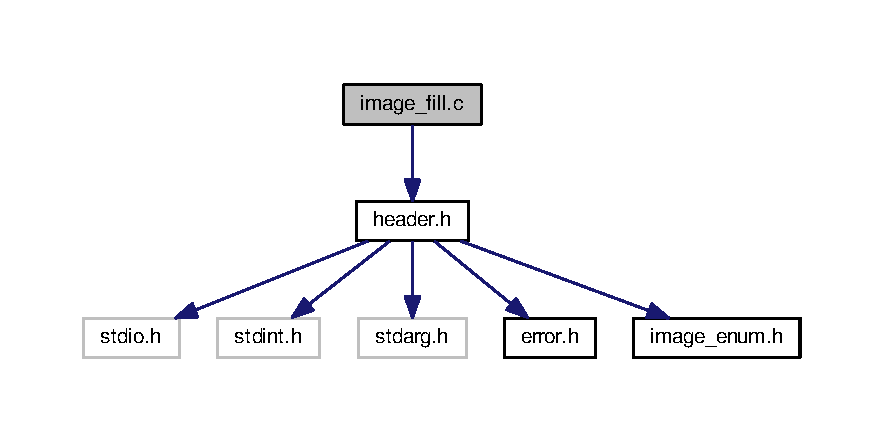
\includegraphics[width=350pt]{image__fill_8c__incl}
\end{center}
\end{figure}
\subsection*{Functions}
\begin{DoxyCompactItemize}
\item 
void \hyperlink{image__fill_8c_a9a114b1f59a4bbe49a1a6c2fd35a60e8}{imel\+\_\+image\+\_\+fill\+\_\+color\+\_\+with\+\_\+color} (\hyperlink{header_8h_ad8298d38a89742ed84029b278c6acee5}{Imel\+Image} $\ast$image, \hyperlink{header_8h_a8b81d020f830e116585b833ea21410c1}{Imel\+Point} $\ast$point, \hyperlink{header_8h_af8a2b40c34eeed326846d0098ea84ec2}{Imel\+Size} tollerance)
\begin{DoxyCompactList}\small\item\em Fill a specified color area with another color. \end{DoxyCompactList}\item 
void \hyperlink{image__fill_8c_a5ce5cafd0a0376534a5896a834d3e273}{imel\+\_\+image\+\_\+fill\+\_\+level\+\_\+with\+\_\+color} (\hyperlink{header_8h_ad8298d38a89742ed84029b278c6acee5}{Imel\+Image} $\ast$image, \hyperlink{header_8h_a8b81d020f830e116585b833ea21410c1}{Imel\+Point} $\ast$point, \hyperlink{header_8h_af8a2b40c34eeed326846d0098ea84ec2}{Imel\+Size} tollerance)
\begin{DoxyCompactList}\small\item\em Fill a specified level area with another color. \end{DoxyCompactList}\item 
void \hyperlink{image__fill_8c_a80afdde2693aef5e71fd7a42d4ef74f3}{imel\+\_\+image\+\_\+fill\+\_\+color\+\_\+with\+\_\+level} (\hyperlink{header_8h_ad8298d38a89742ed84029b278c6acee5}{Imel\+Image} $\ast$image, \hyperlink{header_8h_a8b81d020f830e116585b833ea21410c1}{Imel\+Point} $\ast$point, \hyperlink{header_8h_af8a2b40c34eeed326846d0098ea84ec2}{Imel\+Size} tollerance)
\begin{DoxyCompactList}\small\item\em Fill a specified color area with another level. \end{DoxyCompactList}\item 
void \hyperlink{image__fill_8c_aed5923cf52cf969bf9fc39f6103a0c00}{imel\+\_\+image\+\_\+fill\+\_\+level\+\_\+with\+\_\+level} (\hyperlink{header_8h_ad8298d38a89742ed84029b278c6acee5}{Imel\+Image} $\ast$image, \hyperlink{header_8h_a8b81d020f830e116585b833ea21410c1}{Imel\+Point} $\ast$point, \hyperlink{header_8h_af8a2b40c34eeed326846d0098ea84ec2}{Imel\+Size} tollerance)
\begin{DoxyCompactList}\small\item\em Fill a specified level area with another level. \end{DoxyCompactList}\end{DoxyCompactItemize}


\subsection{Detailed Description}
This file contains functions to fill areas of an image. 

\begin{DoxyAuthor}{Author}
Davide Francesco Merico 
\end{DoxyAuthor}


\subsection{Function Documentation}
\index{image\+\_\+fill.\+c@{image\+\_\+fill.\+c}!imel\+\_\+image\+\_\+fill\+\_\+color\+\_\+with\+\_\+color@{imel\+\_\+image\+\_\+fill\+\_\+color\+\_\+with\+\_\+color}}
\index{imel\+\_\+image\+\_\+fill\+\_\+color\+\_\+with\+\_\+color@{imel\+\_\+image\+\_\+fill\+\_\+color\+\_\+with\+\_\+color}!image\+\_\+fill.\+c@{image\+\_\+fill.\+c}}
\subsubsection[{\texorpdfstring{imel\+\_\+image\+\_\+fill\+\_\+color\+\_\+with\+\_\+color(\+Imel\+Image $\ast$image, Imel\+Point $\ast$point, Imel\+Size tollerance)}{imel_image_fill_color_with_color(ImelImage *image, ImelPoint *point, ImelSize tollerance)}}]{\setlength{\rightskip}{0pt plus 5cm}void imel\+\_\+image\+\_\+fill\+\_\+color\+\_\+with\+\_\+color (
\begin{DoxyParamCaption}
\item[{{\bf Imel\+Image} $\ast$}]{image, }
\item[{{\bf Imel\+Point} $\ast$}]{point, }
\item[{{\bf Imel\+Size}}]{tollerance}
\end{DoxyParamCaption}
)}\hypertarget{image__fill_8c_a9a114b1f59a4bbe49a1a6c2fd35a60e8}{}\label{image__fill_8c_a9a114b1f59a4bbe49a1a6c2fd35a60e8}


Fill a specified color area with another color. 

This function fill a color area with another color.


\begin{DoxyParams}{Parameters}
{\em image} & Image where area to fill exist. \\
\hline
{\em point} & Coordinate of the position to start to fill and the new color value. \\
\hline
{\em tollerance} & Tollerance to find the next pixel to fill\\
\hline
\end{DoxyParams}
\begin{DoxySeeAlso}{See also}
\hyperlink{point_8c_a20c030176364130df49237e29b69308c}{imel\+\_\+point\+\_\+new} 
\end{DoxySeeAlso}
\index{image\+\_\+fill.\+c@{image\+\_\+fill.\+c}!imel\+\_\+image\+\_\+fill\+\_\+color\+\_\+with\+\_\+level@{imel\+\_\+image\+\_\+fill\+\_\+color\+\_\+with\+\_\+level}}
\index{imel\+\_\+image\+\_\+fill\+\_\+color\+\_\+with\+\_\+level@{imel\+\_\+image\+\_\+fill\+\_\+color\+\_\+with\+\_\+level}!image\+\_\+fill.\+c@{image\+\_\+fill.\+c}}
\subsubsection[{\texorpdfstring{imel\+\_\+image\+\_\+fill\+\_\+color\+\_\+with\+\_\+level(\+Imel\+Image $\ast$image, Imel\+Point $\ast$point, Imel\+Size tollerance)}{imel_image_fill_color_with_level(ImelImage *image, ImelPoint *point, ImelSize tollerance)}}]{\setlength{\rightskip}{0pt plus 5cm}void imel\+\_\+image\+\_\+fill\+\_\+color\+\_\+with\+\_\+level (
\begin{DoxyParamCaption}
\item[{{\bf Imel\+Image} $\ast$}]{image, }
\item[{{\bf Imel\+Point} $\ast$}]{point, }
\item[{{\bf Imel\+Size}}]{tollerance}
\end{DoxyParamCaption}
)}\hypertarget{image__fill_8c_a80afdde2693aef5e71fd7a42d4ef74f3}{}\label{image__fill_8c_a80afdde2693aef5e71fd7a42d4ef74f3}


Fill a specified color area with another level. 

This function fill a specified color area with another level.


\begin{DoxyParams}{Parameters}
{\em image} & Image where area to fill exist. \\
\hline
{\em point} & Coordinate of the position to start to fill and new level value. \\
\hline
{\em tollerance} & Tollerance to find the next pixel to fill\\
\hline
\end{DoxyParams}
\begin{DoxySeeAlso}{See also}
\hyperlink{point_8c_a20c030176364130df49237e29b69308c}{imel\+\_\+point\+\_\+new} 
\end{DoxySeeAlso}
\index{image\+\_\+fill.\+c@{image\+\_\+fill.\+c}!imel\+\_\+image\+\_\+fill\+\_\+level\+\_\+with\+\_\+color@{imel\+\_\+image\+\_\+fill\+\_\+level\+\_\+with\+\_\+color}}
\index{imel\+\_\+image\+\_\+fill\+\_\+level\+\_\+with\+\_\+color@{imel\+\_\+image\+\_\+fill\+\_\+level\+\_\+with\+\_\+color}!image\+\_\+fill.\+c@{image\+\_\+fill.\+c}}
\subsubsection[{\texorpdfstring{imel\+\_\+image\+\_\+fill\+\_\+level\+\_\+with\+\_\+color(\+Imel\+Image $\ast$image, Imel\+Point $\ast$point, Imel\+Size tollerance)}{imel_image_fill_level_with_color(ImelImage *image, ImelPoint *point, ImelSize tollerance)}}]{\setlength{\rightskip}{0pt plus 5cm}void imel\+\_\+image\+\_\+fill\+\_\+level\+\_\+with\+\_\+color (
\begin{DoxyParamCaption}
\item[{{\bf Imel\+Image} $\ast$}]{image, }
\item[{{\bf Imel\+Point} $\ast$}]{point, }
\item[{{\bf Imel\+Size}}]{tollerance}
\end{DoxyParamCaption}
)}\hypertarget{image__fill_8c_a5ce5cafd0a0376534a5896a834d3e273}{}\label{image__fill_8c_a5ce5cafd0a0376534a5896a834d3e273}


Fill a specified level area with another color. 

This function fill a specified level area with another color.


\begin{DoxyParams}{Parameters}
{\em image} & Image where area to fill exist. \\
\hline
{\em point} & Coordinate of the position to start to fill and the new color value. \\
\hline
{\em tollerance} & Tollerance to find the next pixel to fill\\
\hline
\end{DoxyParams}
\begin{DoxySeeAlso}{See also}
\hyperlink{point_8c_a20c030176364130df49237e29b69308c}{imel\+\_\+point\+\_\+new} 
\end{DoxySeeAlso}
\index{image\+\_\+fill.\+c@{image\+\_\+fill.\+c}!imel\+\_\+image\+\_\+fill\+\_\+level\+\_\+with\+\_\+level@{imel\+\_\+image\+\_\+fill\+\_\+level\+\_\+with\+\_\+level}}
\index{imel\+\_\+image\+\_\+fill\+\_\+level\+\_\+with\+\_\+level@{imel\+\_\+image\+\_\+fill\+\_\+level\+\_\+with\+\_\+level}!image\+\_\+fill.\+c@{image\+\_\+fill.\+c}}
\subsubsection[{\texorpdfstring{imel\+\_\+image\+\_\+fill\+\_\+level\+\_\+with\+\_\+level(\+Imel\+Image $\ast$image, Imel\+Point $\ast$point, Imel\+Size tollerance)}{imel_image_fill_level_with_level(ImelImage *image, ImelPoint *point, ImelSize tollerance)}}]{\setlength{\rightskip}{0pt plus 5cm}void imel\+\_\+image\+\_\+fill\+\_\+level\+\_\+with\+\_\+level (
\begin{DoxyParamCaption}
\item[{{\bf Imel\+Image} $\ast$}]{image, }
\item[{{\bf Imel\+Point} $\ast$}]{point, }
\item[{{\bf Imel\+Size}}]{tollerance}
\end{DoxyParamCaption}
)}\hypertarget{image__fill_8c_aed5923cf52cf969bf9fc39f6103a0c00}{}\label{image__fill_8c_aed5923cf52cf969bf9fc39f6103a0c00}


Fill a specified level area with another level. 

This function fill a specified level area with another level.


\begin{DoxyParams}{Parameters}
{\em image} & Image where area to fill exist. \\
\hline
{\em point} & Coordinate of the position to start to fill and new level value. \\
\hline
{\em tollerance} & Tollerance to find the next pixel to fill\\
\hline
\end{DoxyParams}
\begin{DoxySeeAlso}{See also}
\hyperlink{point_8c_a20c030176364130df49237e29b69308c}{imel\+\_\+point\+\_\+new} 
\end{DoxySeeAlso}

\hypertarget{image__new__from_8c}{}\section{image\+\_\+new\+\_\+from.\+c File Reference}
\label{image__new__from_8c}\index{image\+\_\+new\+\_\+from.\+c@{image\+\_\+new\+\_\+from.\+c}}


This file contains function to load different image format.  


{\ttfamily \#include $<$string.\+h$>$}\\*
{\ttfamily \#include $<$errno.\+h$>$}\\*
{\ttfamily \#include $<$stdlib.\+h$>$}\\*
{\ttfamily \#include $<$math.\+h$>$}\\*
{\ttfamily \#include $<$Free\+Image.\+h$>$}\\*
{\ttfamily \#include \char`\"{}header.\+h\char`\"{}}\\*
Include dependency graph for image\+\_\+new\+\_\+from.\+c\+:
\nopagebreak
\begin{figure}[H]
\begin{center}
\leavevmode
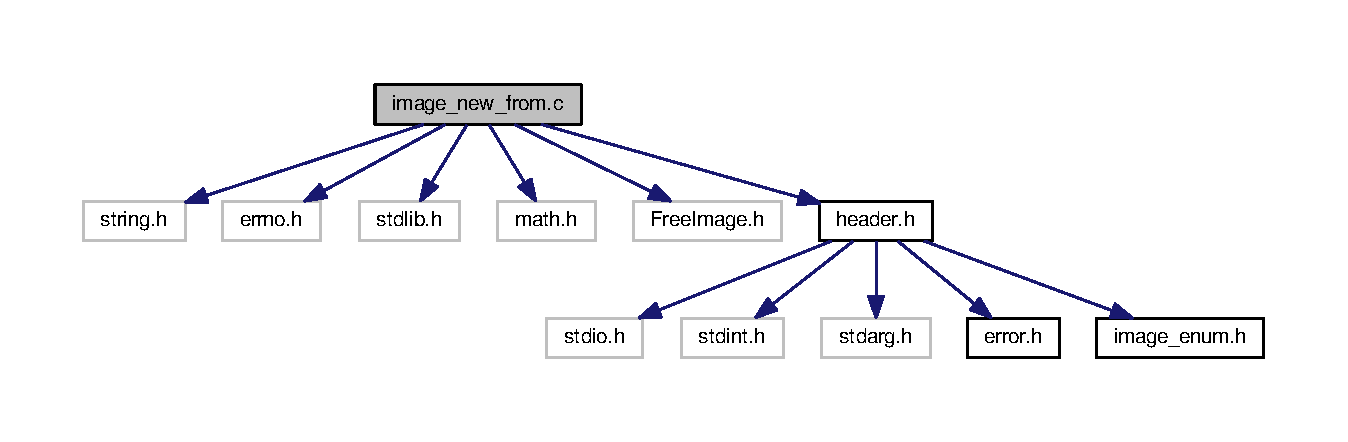
\includegraphics[width=350pt]{image__new__from_8c__incl}
\end{center}
\end{figure}
\subsection*{Functions}
\begin{DoxyCompactItemize}
\item 
\hyperlink{header_8h_ad8298d38a89742ed84029b278c6acee5}{Imel\+Image} $\ast$ \hyperlink{image__new__from_8c_ac246442f4d545cbeec0ed6ad138f8138}{imel\+\_\+image\+\_\+new\+\_\+from\+\_\+imel} (const char $\ast$filename, \hyperlink{header_8h_abe31dcaa4b6683d315101c48b1ca2a56}{Imel\+Error} $\ast$error)
\begin{DoxyCompactList}\small\item\em Load an I\+M\+EL image from a file name. \end{DoxyCompactList}\item 
\hyperlink{header_8h_ad8298d38a89742ed84029b278c6acee5}{Imel\+Image} $\ast$ \hyperlink{image__new__from_8c_a829d009a068dcf5d89326d6180f5a9f9}{imel\+\_\+image\+\_\+new\+\_\+from\+\_\+imel\+\_\+handle} (F\+I\+LE $\ast$of, \hyperlink{header_8h_abe31dcaa4b6683d315101c48b1ca2a56}{Imel\+Error} $\ast$error)
\begin{DoxyCompactList}\small\item\em Load an I\+M\+EL image from an already open file. \end{DoxyCompactList}\item 
\hyperlink{header_8h_ad8298d38a89742ed84029b278c6acee5}{Imel\+Image} $\ast$ \hyperlink{image__new__from_8c_a3dff128ff4d31d07d9cb4c29fe798f9e}{imel\+\_\+image\+\_\+new\+\_\+from\+\_\+raw} (const char $\ast$filename, \hyperlink{header_8h_af8a2b40c34eeed326846d0098ea84ec2}{Imel\+Size} width, \hyperlink{header_8h_af8a2b40c34eeed326846d0098ea84ec2}{Imel\+Size} height, int bits\+\_\+red, int bits\+\_\+green, int bits\+\_\+blue, int bits\+\_\+level, \hyperlink{header_8h_abe31dcaa4b6683d315101c48b1ca2a56}{Imel\+Error} $\ast$error)
\begin{DoxyCompactList}\small\item\em Load a raw image from file name. \end{DoxyCompactList}\item 
\hyperlink{header_8h_ad8298d38a89742ed84029b278c6acee5}{Imel\+Image} $\ast$ \hyperlink{image__new__from_8c_a0e52940557ae0c41e132db213a70afd4}{imel\+\_\+image\+\_\+new\+\_\+from\+\_\+jpeg} (const char $\ast$filename, long int level, \hyperlink{image__enum_8h_a26855928d18f44de0b410c4e481215d0}{Imel\+Jpeg\+Load\+Flags} load\+\_\+flags, \hyperlink{header_8h_abe31dcaa4b6683d315101c48b1ca2a56}{Imel\+Error} $\ast$error)
\begin{DoxyCompactList}\small\item\em Load a J\+P\+EG image from a file name. \end{DoxyCompactList}\item 
\hyperlink{header_8h_ad8298d38a89742ed84029b278c6acee5}{Imel\+Image} $\ast$ \hyperlink{image__new__from_8c_a255854b1e1dc8be8445f666894332145}{imel\+\_\+image\+\_\+new\+\_\+from\+\_\+jpeg\+\_\+handle} (F\+I\+LE $\ast$file, long int level, \hyperlink{image__enum_8h_a26855928d18f44de0b410c4e481215d0}{Imel\+Jpeg\+Load\+Flags} load\+\_\+flags, \hyperlink{header_8h_abe31dcaa4b6683d315101c48b1ca2a56}{Imel\+Error} $\ast$error)
\begin{DoxyCompactList}\small\item\em Load a J\+P\+EG image from an already open file. \end{DoxyCompactList}\item 
\hyperlink{header_8h_ad8298d38a89742ed84029b278c6acee5}{Imel\+Image} $\ast$ \hyperlink{image__new__from_8c_a91fe1c254d77bb29cf84d9e12a747727}{imel\+\_\+image\+\_\+new\+\_\+from\+\_\+jpeg\+\_\+memory} (uint8\+\_\+t $\ast$memory, uint32\+\_\+t length, long int level, \hyperlink{image__enum_8h_a26855928d18f44de0b410c4e481215d0}{Imel\+Jpeg\+Load\+Flags} load\+\_\+flags, \hyperlink{header_8h_abe31dcaa4b6683d315101c48b1ca2a56}{Imel\+Error} $\ast$error)
\begin{DoxyCompactList}\small\item\em Load a J\+P\+EG image from an one loaded in memory. \end{DoxyCompactList}\item 
\hyperlink{header_8h_ad8298d38a89742ed84029b278c6acee5}{Imel\+Image} $\ast$ \hyperlink{image__new__from_8c_a479e487f5bf0995932ed8a5ec05cd030}{imel\+\_\+image\+\_\+new\+\_\+from\+\_\+png} (const char $\ast$filename, long int level, \hyperlink{image__enum_8h_a9b61323ba1a40fa051e89e4f09d4cd12}{Imel\+Png\+Load\+Flags} load\+\_\+flags, \hyperlink{header_8h_abe31dcaa4b6683d315101c48b1ca2a56}{Imel\+Error} $\ast$error)
\begin{DoxyCompactList}\small\item\em Load a P\+NG image from a file name. \end{DoxyCompactList}\item 
\hyperlink{header_8h_ad8298d38a89742ed84029b278c6acee5}{Imel\+Image} $\ast$ \hyperlink{image__new__from_8c_acf9c896ceea45e10a991780407c3c259}{imel\+\_\+image\+\_\+new\+\_\+from\+\_\+png\+\_\+handle} (F\+I\+LE $\ast$file, long int level, \hyperlink{image__enum_8h_a9b61323ba1a40fa051e89e4f09d4cd12}{Imel\+Png\+Load\+Flags} load\+\_\+flags, \hyperlink{header_8h_abe31dcaa4b6683d315101c48b1ca2a56}{Imel\+Error} $\ast$error)
\begin{DoxyCompactList}\small\item\em Load a P\+NG image from an already open file. \end{DoxyCompactList}\item 
\hyperlink{header_8h_ad8298d38a89742ed84029b278c6acee5}{Imel\+Image} $\ast$ \hyperlink{image__new__from_8c_a834d3fef3f5336c6d294e84afb0f0a62}{imel\+\_\+image\+\_\+new\+\_\+from\+\_\+png\+\_\+memory} (uint8\+\_\+t $\ast$memory, uint32\+\_\+t length, long int level, \hyperlink{image__enum_8h_a9b61323ba1a40fa051e89e4f09d4cd12}{Imel\+Png\+Load\+Flags} load\+\_\+flags, \hyperlink{header_8h_abe31dcaa4b6683d315101c48b1ca2a56}{Imel\+Error} $\ast$error)
\begin{DoxyCompactList}\small\item\em Load a P\+NG image from an one loaded in memory. \end{DoxyCompactList}\item 
\hyperlink{header_8h_ad8298d38a89742ed84029b278c6acee5}{Imel\+Image} $\ast$ \hyperlink{image__new__from_8c_a00fa94d7b7737a3112030ae792479662}{imel\+\_\+image\+\_\+new\+\_\+from\+\_\+tiff} (const char $\ast$filename, long int level, \hyperlink{image__enum_8h_a6a075ca8fec1ae793bf2806e6dccc63a}{Imel\+Tiff\+Load\+Flags} load\+\_\+flags, \hyperlink{header_8h_abe31dcaa4b6683d315101c48b1ca2a56}{Imel\+Error} $\ast$error)
\begin{DoxyCompactList}\small\item\em Load a T\+I\+FF image from a file name. \end{DoxyCompactList}\item 
\hyperlink{header_8h_ad8298d38a89742ed84029b278c6acee5}{Imel\+Image} $\ast$ \hyperlink{image__new__from_8c_af02f902b678626b6e015209d0dcbb3ba}{imel\+\_\+image\+\_\+new\+\_\+from\+\_\+tiff\+\_\+handle} (F\+I\+LE $\ast$file, long int level, \hyperlink{image__enum_8h_a6a075ca8fec1ae793bf2806e6dccc63a}{Imel\+Tiff\+Load\+Flags} load\+\_\+flags, \hyperlink{header_8h_abe31dcaa4b6683d315101c48b1ca2a56}{Imel\+Error} $\ast$error)
\begin{DoxyCompactList}\small\item\em Load a T\+I\+FF image from an already open file. \end{DoxyCompactList}\item 
\hyperlink{header_8h_ad8298d38a89742ed84029b278c6acee5}{Imel\+Image} $\ast$ \hyperlink{image__new__from_8c_a6f49e56a0ea5eeb96be3381dd8e6813b}{imel\+\_\+image\+\_\+new\+\_\+from\+\_\+tiff\+\_\+memory} (uint8\+\_\+t $\ast$memory, uint32\+\_\+t length, long int level, \hyperlink{image__enum_8h_a6a075ca8fec1ae793bf2806e6dccc63a}{Imel\+Tiff\+Load\+Flags} load\+\_\+flags, \hyperlink{header_8h_abe31dcaa4b6683d315101c48b1ca2a56}{Imel\+Error} $\ast$error)
\begin{DoxyCompactList}\small\item\em Load a T\+I\+FF image from an one loaded in memory. \end{DoxyCompactList}\item 
\hyperlink{header_8h_ad8298d38a89742ed84029b278c6acee5}{Imel\+Image} $\ast$ \hyperlink{image__new__from_8c_aeb3657cf4496b84f21638bd966a8c63a}{imel\+\_\+image\+\_\+new\+\_\+from\+\_\+bmp} (const char $\ast$filename, long int level, \hyperlink{header_8h_abe31dcaa4b6683d315101c48b1ca2a56}{Imel\+Error} $\ast$error)
\begin{DoxyCompactList}\small\item\em Load a B\+MP image from a file name. \end{DoxyCompactList}\item 
\hyperlink{header_8h_ad8298d38a89742ed84029b278c6acee5}{Imel\+Image} $\ast$ \hyperlink{image__new__from_8c_a984d4dcb07631d2cf9664a9abfaf0ca4}{imel\+\_\+image\+\_\+new\+\_\+from\+\_\+bmp\+\_\+handle} (F\+I\+LE $\ast$file, long int level, \hyperlink{header_8h_abe31dcaa4b6683d315101c48b1ca2a56}{Imel\+Error} $\ast$error)
\begin{DoxyCompactList}\small\item\em Load a B\+MP image from an already open file. \end{DoxyCompactList}\item 
\hyperlink{header_8h_ad8298d38a89742ed84029b278c6acee5}{Imel\+Image} $\ast$ \hyperlink{image__new__from_8c_a74f243ec0ad73f61be448f1f3747af37}{imel\+\_\+image\+\_\+new\+\_\+from\+\_\+bmp\+\_\+memory} (uint8\+\_\+t $\ast$memory, uint32\+\_\+t length, long int level, \hyperlink{header_8h_abe31dcaa4b6683d315101c48b1ca2a56}{Imel\+Error} $\ast$error)
\begin{DoxyCompactList}\small\item\em Load a B\+MP image from an one loaded in memory. \end{DoxyCompactList}\item 
\hyperlink{header_8h_ad8298d38a89742ed84029b278c6acee5}{Imel\+Image} $\ast$ \hyperlink{image__new__from_8c_a367a48d31d447f92db756f4e2e29d498}{imel\+\_\+image\+\_\+new\+\_\+from\+\_\+cut} (const char $\ast$filename, long int level, \hyperlink{header_8h_abe31dcaa4b6683d315101c48b1ca2a56}{Imel\+Error} $\ast$error)
\begin{DoxyCompactList}\small\item\em Load a C\+UT image from a file name. \end{DoxyCompactList}\item 
\hyperlink{header_8h_ad8298d38a89742ed84029b278c6acee5}{Imel\+Image} $\ast$ \hyperlink{image__new__from_8c_a9fb5c996b3b1d6b8c1ac3260caf651f6}{imel\+\_\+image\+\_\+new\+\_\+from\+\_\+cut\+\_\+handle} (F\+I\+LE $\ast$file, long int level, \hyperlink{header_8h_abe31dcaa4b6683d315101c48b1ca2a56}{Imel\+Error} $\ast$error)
\begin{DoxyCompactList}\small\item\em Load a C\+UT image from an already open file. \end{DoxyCompactList}\item 
\hyperlink{header_8h_ad8298d38a89742ed84029b278c6acee5}{Imel\+Image} $\ast$ \hyperlink{image__new__from_8c_ab474e2eefa8f43d0ae8d5d9bea743bbd}{imel\+\_\+image\+\_\+new\+\_\+from\+\_\+cut\+\_\+memory} (uint8\+\_\+t $\ast$memory, uint32\+\_\+t length, long int level, \hyperlink{header_8h_abe31dcaa4b6683d315101c48b1ca2a56}{Imel\+Error} $\ast$error)
\begin{DoxyCompactList}\small\item\em Load a C\+UT image from an one loaded in memory. \end{DoxyCompactList}\item 
\hyperlink{header_8h_ad8298d38a89742ed84029b278c6acee5}{Imel\+Image} $\ast$ \hyperlink{image__new__from_8c_a6377df7548d28a47f326e91e63db8ab5}{imel\+\_\+image\+\_\+new\+\_\+from\+\_\+dds} (const char $\ast$filename, long int level, \hyperlink{header_8h_abe31dcaa4b6683d315101c48b1ca2a56}{Imel\+Error} $\ast$error)
\begin{DoxyCompactList}\small\item\em Load a D\+DS image from a file name. \end{DoxyCompactList}\item 
\hyperlink{header_8h_ad8298d38a89742ed84029b278c6acee5}{Imel\+Image} $\ast$ \hyperlink{image__new__from_8c_a6aaf149cdf4b6407bec2547619730712}{imel\+\_\+image\+\_\+new\+\_\+from\+\_\+dds\+\_\+handle} (F\+I\+LE $\ast$file, long int level, \hyperlink{header_8h_abe31dcaa4b6683d315101c48b1ca2a56}{Imel\+Error} $\ast$error)
\begin{DoxyCompactList}\small\item\em Load a D\+DS image from an already open file. \end{DoxyCompactList}\item 
\hyperlink{header_8h_ad8298d38a89742ed84029b278c6acee5}{Imel\+Image} $\ast$ \hyperlink{image__new__from_8c_ae301b9ef2415e7bd7c1684345022cd26}{imel\+\_\+image\+\_\+new\+\_\+from\+\_\+dds\+\_\+memory} (uint8\+\_\+t $\ast$memory, uint32\+\_\+t length, long int level, \hyperlink{header_8h_abe31dcaa4b6683d315101c48b1ca2a56}{Imel\+Error} $\ast$error)
\begin{DoxyCompactList}\small\item\em Load a D\+DS image from an one loaded in memory. \end{DoxyCompactList}\item 
\hyperlink{header_8h_ad8298d38a89742ed84029b278c6acee5}{Imel\+Image} $\ast$ \hyperlink{image__new__from_8c_a77997c2ae5d2ad79bcd620823e2cbed1}{imel\+\_\+image\+\_\+new\+\_\+from\+\_\+xpm} (const char $\ast$filename, long int level, \hyperlink{header_8h_abe31dcaa4b6683d315101c48b1ca2a56}{Imel\+Error} $\ast$error)
\begin{DoxyCompactList}\small\item\em Load a X\+PM image from a file name. \end{DoxyCompactList}\item 
\hyperlink{header_8h_ad8298d38a89742ed84029b278c6acee5}{Imel\+Image} $\ast$ \hyperlink{image__new__from_8c_a2dcf8c0d9537ddac653e9c28926d1de9}{imel\+\_\+image\+\_\+new\+\_\+from\+\_\+xpm\+\_\+handle} (F\+I\+LE $\ast$file, long int level, \hyperlink{header_8h_abe31dcaa4b6683d315101c48b1ca2a56}{Imel\+Error} $\ast$error)
\begin{DoxyCompactList}\small\item\em Load a X\+PM image from an already open file. \end{DoxyCompactList}\item 
\hyperlink{header_8h_ad8298d38a89742ed84029b278c6acee5}{Imel\+Image} $\ast$ \hyperlink{image__new__from_8c_aea6c094befb71f918b22c5e7fd00ca0e}{imel\+\_\+image\+\_\+new\+\_\+from\+\_\+xpm\+\_\+memory} (uint8\+\_\+t $\ast$memory, uint32\+\_\+t length, long int level, \hyperlink{header_8h_abe31dcaa4b6683d315101c48b1ca2a56}{Imel\+Error} $\ast$error)
\begin{DoxyCompactList}\small\item\em Load a X\+PM image from an one loaded in memory. \end{DoxyCompactList}\item 
\hyperlink{header_8h_ad8298d38a89742ed84029b278c6acee5}{Imel\+Image} $\ast$ \hyperlink{image__new__from_8c_af96ed9a8d082c21ed471ee7da5e00e92}{imel\+\_\+image\+\_\+new\+\_\+from\+\_\+xbm} (const char $\ast$filename, long int level, \hyperlink{header_8h_abe31dcaa4b6683d315101c48b1ca2a56}{Imel\+Error} $\ast$error)
\begin{DoxyCompactList}\small\item\em Load a X\+BM image from a file name. \end{DoxyCompactList}\item 
\hyperlink{header_8h_ad8298d38a89742ed84029b278c6acee5}{Imel\+Image} $\ast$ \hyperlink{image__new__from_8c_a9fdae5f0c78624c379de8e842e05c142}{imel\+\_\+image\+\_\+new\+\_\+from\+\_\+xbm\+\_\+handle} (F\+I\+LE $\ast$file, long int level, \hyperlink{header_8h_abe31dcaa4b6683d315101c48b1ca2a56}{Imel\+Error} $\ast$error)
\begin{DoxyCompactList}\small\item\em Load a X\+BM image from an already open file. \end{DoxyCompactList}\item 
\hyperlink{header_8h_ad8298d38a89742ed84029b278c6acee5}{Imel\+Image} $\ast$ \hyperlink{image__new__from_8c_a87f01e8b375d99ef22e7d8a0b6255e4b}{imel\+\_\+image\+\_\+new\+\_\+from\+\_\+xbm\+\_\+memory} (uint8\+\_\+t $\ast$memory, uint32\+\_\+t length, long int level, \hyperlink{header_8h_abe31dcaa4b6683d315101c48b1ca2a56}{Imel\+Error} $\ast$error)
\begin{DoxyCompactList}\small\item\em Load a X\+BM image from an one loaded in memory. \end{DoxyCompactList}\item 
\hyperlink{header_8h_ad8298d38a89742ed84029b278c6acee5}{Imel\+Image} $\ast$ \hyperlink{image__new__from_8c_a7b389f1d8a2b00586511944742f13869}{imel\+\_\+image\+\_\+new\+\_\+from\+\_\+sgi} (const char $\ast$filename, long int level, \hyperlink{header_8h_abe31dcaa4b6683d315101c48b1ca2a56}{Imel\+Error} $\ast$error)
\begin{DoxyCompactList}\small\item\em Load a S\+GI image from a file name. \end{DoxyCompactList}\item 
\hyperlink{header_8h_ad8298d38a89742ed84029b278c6acee5}{Imel\+Image} $\ast$ \hyperlink{image__new__from_8c_ad64e2266e10b7bad9a95267df80d9ed3}{imel\+\_\+image\+\_\+new\+\_\+from\+\_\+sgi\+\_\+handle} (F\+I\+LE $\ast$file, long int level, \hyperlink{header_8h_abe31dcaa4b6683d315101c48b1ca2a56}{Imel\+Error} $\ast$error)
\begin{DoxyCompactList}\small\item\em Load a S\+GI image from an already open file. \end{DoxyCompactList}\item 
\hyperlink{header_8h_ad8298d38a89742ed84029b278c6acee5}{Imel\+Image} $\ast$ \hyperlink{image__new__from_8c_aebf054c69a9e2d08a4ea9ad90633eeae}{imel\+\_\+image\+\_\+new\+\_\+from\+\_\+sgi\+\_\+memory} (uint8\+\_\+t $\ast$memory, uint32\+\_\+t length, long int level, \hyperlink{header_8h_abe31dcaa4b6683d315101c48b1ca2a56}{Imel\+Error} $\ast$error)
\begin{DoxyCompactList}\small\item\em Load a S\+GI image from an one loaded in memory. \end{DoxyCompactList}\item 
\hyperlink{header_8h_ad8298d38a89742ed84029b278c6acee5}{Imel\+Image} $\ast$ \hyperlink{image__new__from_8c_a4a33044675007c2f73212ffa0ff5a9a8}{imel\+\_\+image\+\_\+new\+\_\+from\+\_\+wbmp} (const char $\ast$filename, long int level, \hyperlink{header_8h_abe31dcaa4b6683d315101c48b1ca2a56}{Imel\+Error} $\ast$error)
\begin{DoxyCompactList}\small\item\em Load a W\+B\+MP image from a file name. \end{DoxyCompactList}\item 
\hyperlink{header_8h_ad8298d38a89742ed84029b278c6acee5}{Imel\+Image} $\ast$ \hyperlink{image__new__from_8c_a320088d1d62a490ad2c2456ec69e9d5e}{imel\+\_\+image\+\_\+new\+\_\+from\+\_\+wbmp\+\_\+handle} (F\+I\+LE $\ast$file, long int level, \hyperlink{header_8h_abe31dcaa4b6683d315101c48b1ca2a56}{Imel\+Error} $\ast$error)
\begin{DoxyCompactList}\small\item\em Load a W\+B\+MP image from an already open file. \end{DoxyCompactList}\item 
\hyperlink{header_8h_ad8298d38a89742ed84029b278c6acee5}{Imel\+Image} $\ast$ \hyperlink{image__new__from_8c_a6c7761ded21860b2d070f0528a126c8f}{imel\+\_\+image\+\_\+new\+\_\+from\+\_\+wbmp\+\_\+memory} (uint8\+\_\+t $\ast$memory, uint32\+\_\+t length, long int level, \hyperlink{header_8h_abe31dcaa4b6683d315101c48b1ca2a56}{Imel\+Error} $\ast$error)
\begin{DoxyCompactList}\small\item\em Load a W\+B\+MP image from an one loaded in memory. \end{DoxyCompactList}\item 
\hyperlink{header_8h_ad8298d38a89742ed84029b278c6acee5}{Imel\+Image} $\ast$ \hyperlink{image__new__from_8c_afcd4cb82240f0154e28c2c49ccee36eb}{imel\+\_\+image\+\_\+new\+\_\+from\+\_\+hdr} (const char $\ast$filename, long int level, \hyperlink{header_8h_abe31dcaa4b6683d315101c48b1ca2a56}{Imel\+Error} $\ast$error)
\begin{DoxyCompactList}\small\item\em Load a H\+DR image from a file name. \end{DoxyCompactList}\item 
\hyperlink{header_8h_ad8298d38a89742ed84029b278c6acee5}{Imel\+Image} $\ast$ \hyperlink{image__new__from_8c_a7645fa3d66aa4afe310804c0befb6788}{imel\+\_\+image\+\_\+new\+\_\+from\+\_\+hdr\+\_\+handle} (F\+I\+LE $\ast$file, long int level, \hyperlink{header_8h_abe31dcaa4b6683d315101c48b1ca2a56}{Imel\+Error} $\ast$error)
\begin{DoxyCompactList}\small\item\em Load a H\+DR image from an already open file. \end{DoxyCompactList}\item 
\hyperlink{header_8h_ad8298d38a89742ed84029b278c6acee5}{Imel\+Image} $\ast$ \hyperlink{image__new__from_8c_a71106226adf5f0474501b4f83ccefb06}{imel\+\_\+image\+\_\+new\+\_\+from\+\_\+hdr\+\_\+memory} (uint8\+\_\+t $\ast$memory, uint32\+\_\+t length, long int level, \hyperlink{header_8h_abe31dcaa4b6683d315101c48b1ca2a56}{Imel\+Error} $\ast$error)
\begin{DoxyCompactList}\small\item\em Load a H\+DR image from an one loaded in memory. \end{DoxyCompactList}\item 
\hyperlink{header_8h_ad8298d38a89742ed84029b278c6acee5}{Imel\+Image} $\ast$ \hyperlink{image__new__from_8c_a0eef90eff7f912d02f6ed24063f6b27f}{imel\+\_\+image\+\_\+new\+\_\+from\+\_\+psd} (const char $\ast$filename, long int level, \hyperlink{header_8h_abe31dcaa4b6683d315101c48b1ca2a56}{Imel\+Error} $\ast$error)
\begin{DoxyCompactList}\small\item\em Load a P\+SD image from a file name. \end{DoxyCompactList}\item 
\hyperlink{header_8h_ad8298d38a89742ed84029b278c6acee5}{Imel\+Image} $\ast$ \hyperlink{image__new__from_8c_a06a25837ace613bb81963534b5655bba}{imel\+\_\+image\+\_\+new\+\_\+from\+\_\+psd\+\_\+handle} (F\+I\+LE $\ast$file, long int level, \hyperlink{header_8h_abe31dcaa4b6683d315101c48b1ca2a56}{Imel\+Error} $\ast$error)
\begin{DoxyCompactList}\small\item\em Load a P\+SD image from an already open file. \end{DoxyCompactList}\item 
\hyperlink{header_8h_ad8298d38a89742ed84029b278c6acee5}{Imel\+Image} $\ast$ \hyperlink{image__new__from_8c_a5d7fbe5da7a7720933780ac74cc899d3}{imel\+\_\+image\+\_\+new\+\_\+from\+\_\+psd\+\_\+memory} (uint8\+\_\+t $\ast$memory, uint32\+\_\+t length, long int level, \hyperlink{header_8h_abe31dcaa4b6683d315101c48b1ca2a56}{Imel\+Error} $\ast$error)
\begin{DoxyCompactList}\small\item\em Load a P\+SD image from an one loaded in memory. \end{DoxyCompactList}\item 
\hyperlink{header_8h_ad8298d38a89742ed84029b278c6acee5}{Imel\+Image} $\ast$ \hyperlink{image__new__from_8c_abdc82d2f55d47201e28ecdb724e9175f}{imel\+\_\+image\+\_\+new\+\_\+from\+\_\+iff} (const char $\ast$filename, long int level, \hyperlink{header_8h_abe31dcaa4b6683d315101c48b1ca2a56}{Imel\+Error} $\ast$error)
\begin{DoxyCompactList}\small\item\em Load a I\+FF image from a file name. \end{DoxyCompactList}\item 
\hyperlink{header_8h_ad8298d38a89742ed84029b278c6acee5}{Imel\+Image} $\ast$ \hyperlink{image__new__from_8c_af409d9589e6e969f785551399c324bcc}{imel\+\_\+image\+\_\+new\+\_\+from\+\_\+iff\+\_\+handle} (F\+I\+LE $\ast$file, long int level, \hyperlink{header_8h_abe31dcaa4b6683d315101c48b1ca2a56}{Imel\+Error} $\ast$error)
\begin{DoxyCompactList}\small\item\em Load a I\+FF image from an already open file. \end{DoxyCompactList}\item 
\hyperlink{header_8h_ad8298d38a89742ed84029b278c6acee5}{Imel\+Image} $\ast$ \hyperlink{image__new__from_8c_ad041e8a55671b2ae0a46c8f5c6185727}{imel\+\_\+image\+\_\+new\+\_\+from\+\_\+iff\+\_\+memory} (uint8\+\_\+t $\ast$memory, uint32\+\_\+t length, long int level, \hyperlink{header_8h_abe31dcaa4b6683d315101c48b1ca2a56}{Imel\+Error} $\ast$error)
\begin{DoxyCompactList}\small\item\em Load a I\+FF image from an one loaded in memory. \end{DoxyCompactList}\item 
\hyperlink{header_8h_ad8298d38a89742ed84029b278c6acee5}{Imel\+Image} $\ast$ \hyperlink{image__new__from_8c_a45e1d85ceba1e1564cf27a2c71f5c1f8}{imel\+\_\+image\+\_\+new\+\_\+from\+\_\+jng} (const char $\ast$filename, long int level, \hyperlink{header_8h_abe31dcaa4b6683d315101c48b1ca2a56}{Imel\+Error} $\ast$error)
\begin{DoxyCompactList}\small\item\em Load a J\+NG image from a file name. \end{DoxyCompactList}\item 
\hyperlink{header_8h_ad8298d38a89742ed84029b278c6acee5}{Imel\+Image} $\ast$ \hyperlink{image__new__from_8c_af65230bf922e4bf591fd761638f40033}{imel\+\_\+image\+\_\+new\+\_\+from\+\_\+jng\+\_\+handle} (F\+I\+LE $\ast$file, long int level, \hyperlink{header_8h_abe31dcaa4b6683d315101c48b1ca2a56}{Imel\+Error} $\ast$error)
\begin{DoxyCompactList}\small\item\em Load a J\+NG image from an already open file. \end{DoxyCompactList}\item 
\hyperlink{header_8h_ad8298d38a89742ed84029b278c6acee5}{Imel\+Image} $\ast$ \hyperlink{image__new__from_8c_ab889d6697602c04bea03caa6f5135ab6}{imel\+\_\+image\+\_\+new\+\_\+from\+\_\+jng\+\_\+memory} (uint8\+\_\+t $\ast$memory, uint32\+\_\+t length, long int level, \hyperlink{header_8h_abe31dcaa4b6683d315101c48b1ca2a56}{Imel\+Error} $\ast$error)
\begin{DoxyCompactList}\small\item\em Load a J\+NG image from an one loaded in memory. \end{DoxyCompactList}\item 
\hyperlink{header_8h_ad8298d38a89742ed84029b278c6acee5}{Imel\+Image} $\ast$ \hyperlink{image__new__from_8c_a364bd7d10ede0974675cc9af70aa0c44}{imel\+\_\+image\+\_\+new\+\_\+from\+\_\+koala} (const char $\ast$filename, long int level, \hyperlink{header_8h_abe31dcaa4b6683d315101c48b1ca2a56}{Imel\+Error} $\ast$error)
\begin{DoxyCompactList}\small\item\em Load a K\+O\+A\+LA image from a file name. \end{DoxyCompactList}\item 
\hyperlink{header_8h_ad8298d38a89742ed84029b278c6acee5}{Imel\+Image} $\ast$ \hyperlink{image__new__from_8c_a6768f54c2cfc098b6a518973f7a53d28}{imel\+\_\+image\+\_\+new\+\_\+from\+\_\+koala\+\_\+handle} (F\+I\+LE $\ast$file, long int level, \hyperlink{header_8h_abe31dcaa4b6683d315101c48b1ca2a56}{Imel\+Error} $\ast$error)
\begin{DoxyCompactList}\small\item\em Load a K\+O\+A\+LA image from an already open file. \end{DoxyCompactList}\item 
\hyperlink{header_8h_ad8298d38a89742ed84029b278c6acee5}{Imel\+Image} $\ast$ \hyperlink{image__new__from_8c_a5a0acee3aa2b249ea55ed23a66cd1770}{imel\+\_\+image\+\_\+new\+\_\+from\+\_\+koala\+\_\+memory} (uint8\+\_\+t $\ast$memory, uint32\+\_\+t length, long int level, \hyperlink{header_8h_abe31dcaa4b6683d315101c48b1ca2a56}{Imel\+Error} $\ast$error)
\begin{DoxyCompactList}\small\item\em Load a K\+O\+A\+LA image from an one loaded in memory. \end{DoxyCompactList}\item 
\hyperlink{header_8h_ad8298d38a89742ed84029b278c6acee5}{Imel\+Image} $\ast$ \hyperlink{image__new__from_8c_a40bcdd596f25f2373e5e8208b61292e9}{imel\+\_\+image\+\_\+new\+\_\+from\+\_\+mng} (const char $\ast$filename, long int level, \hyperlink{header_8h_abe31dcaa4b6683d315101c48b1ca2a56}{Imel\+Error} $\ast$error)
\begin{DoxyCompactList}\small\item\em Load a M\+NG image from a file name. \end{DoxyCompactList}\item 
\hyperlink{header_8h_ad8298d38a89742ed84029b278c6acee5}{Imel\+Image} $\ast$ \hyperlink{image__new__from_8c_ab18b62a239b8cb2d580c4ab2e702c960}{imel\+\_\+image\+\_\+new\+\_\+from\+\_\+mng\+\_\+handle} (F\+I\+LE $\ast$file, long int level, \hyperlink{header_8h_abe31dcaa4b6683d315101c48b1ca2a56}{Imel\+Error} $\ast$error)
\begin{DoxyCompactList}\small\item\em Load a M\+NG image from an already open file. \end{DoxyCompactList}\item 
\hyperlink{header_8h_ad8298d38a89742ed84029b278c6acee5}{Imel\+Image} $\ast$ \hyperlink{image__new__from_8c_af3d322f11e2facfee1b0bc118f64556b}{imel\+\_\+image\+\_\+new\+\_\+from\+\_\+mng\+\_\+memory} (uint8\+\_\+t $\ast$memory, uint32\+\_\+t length, long int level, \hyperlink{header_8h_abe31dcaa4b6683d315101c48b1ca2a56}{Imel\+Error} $\ast$error)
\begin{DoxyCompactList}\small\item\em Load a M\+NG image from an one loaded in memory. \end{DoxyCompactList}\item 
\hyperlink{header_8h_ad8298d38a89742ed84029b278c6acee5}{Imel\+Image} $\ast$ \hyperlink{image__new__from_8c_aa281bf9846f7c509bd83a77eb656beef}{imel\+\_\+image\+\_\+new\+\_\+from\+\_\+pcx} (const char $\ast$filename, long int level, \hyperlink{header_8h_abe31dcaa4b6683d315101c48b1ca2a56}{Imel\+Error} $\ast$error)
\begin{DoxyCompactList}\small\item\em Load a P\+CX image from a file name. \end{DoxyCompactList}\item 
\hyperlink{header_8h_ad8298d38a89742ed84029b278c6acee5}{Imel\+Image} $\ast$ \hyperlink{image__new__from_8c_aaa3d88d5904712d68fd84c2d2518488c}{imel\+\_\+image\+\_\+new\+\_\+from\+\_\+pcx\+\_\+handle} (F\+I\+LE $\ast$file, long int level, \hyperlink{header_8h_abe31dcaa4b6683d315101c48b1ca2a56}{Imel\+Error} $\ast$error)
\begin{DoxyCompactList}\small\item\em Load a P\+CX image from an already open file. \end{DoxyCompactList}\item 
\hyperlink{header_8h_ad8298d38a89742ed84029b278c6acee5}{Imel\+Image} $\ast$ \hyperlink{image__new__from_8c_a6715d7ecaf4c90d601669288fa5f2652}{imel\+\_\+image\+\_\+new\+\_\+from\+\_\+pcx\+\_\+memory} (uint8\+\_\+t $\ast$memory, uint32\+\_\+t length, long int level, \hyperlink{header_8h_abe31dcaa4b6683d315101c48b1ca2a56}{Imel\+Error} $\ast$error)
\begin{DoxyCompactList}\small\item\em Load a P\+CX image from an one loaded in memory. \end{DoxyCompactList}\item 
\hyperlink{header_8h_ad8298d38a89742ed84029b278c6acee5}{Imel\+Image} $\ast$ \hyperlink{image__new__from_8c_afa3039ec9905047ba7c6215d61ef8d19}{imel\+\_\+image\+\_\+new\+\_\+from\+\_\+pgm} (const char $\ast$filename, long int level, \hyperlink{header_8h_abe31dcaa4b6683d315101c48b1ca2a56}{Imel\+Error} $\ast$error)
\begin{DoxyCompactList}\small\item\em Load a P\+GM image from a file name. \end{DoxyCompactList}\item 
\hyperlink{header_8h_ad8298d38a89742ed84029b278c6acee5}{Imel\+Image} $\ast$ \hyperlink{image__new__from_8c_a5e891a501730c0a89e69d6d308ef2571}{imel\+\_\+image\+\_\+new\+\_\+from\+\_\+pgm\+\_\+handle} (F\+I\+LE $\ast$file, long int level, \hyperlink{header_8h_abe31dcaa4b6683d315101c48b1ca2a56}{Imel\+Error} $\ast$error)
\begin{DoxyCompactList}\small\item\em Load a P\+GM image from an already open file. \end{DoxyCompactList}\item 
\hyperlink{header_8h_ad8298d38a89742ed84029b278c6acee5}{Imel\+Image} $\ast$ \hyperlink{image__new__from_8c_accc200fda5590848d1af786c255b870d}{imel\+\_\+image\+\_\+new\+\_\+from\+\_\+pgm\+\_\+memory} (uint8\+\_\+t $\ast$memory, uint32\+\_\+t length, long int level, \hyperlink{header_8h_abe31dcaa4b6683d315101c48b1ca2a56}{Imel\+Error} $\ast$error)
\begin{DoxyCompactList}\small\item\em Load a P\+GM image from an one loaded in memory. \end{DoxyCompactList}\item 
\hyperlink{header_8h_ad8298d38a89742ed84029b278c6acee5}{Imel\+Image} $\ast$ \hyperlink{image__new__from_8c_a295f0971f7087b20e68265523d31439d}{imel\+\_\+image\+\_\+new\+\_\+from\+\_\+pgmraw} (const char $\ast$filename, long int level, \hyperlink{header_8h_abe31dcaa4b6683d315101c48b1ca2a56}{Imel\+Error} $\ast$error)
\begin{DoxyCompactList}\small\item\em Load a raw P\+GM image from a file name. \end{DoxyCompactList}\item 
\hyperlink{header_8h_ad8298d38a89742ed84029b278c6acee5}{Imel\+Image} $\ast$ \hyperlink{image__new__from_8c_a88c24965fb893165fd0a4535a7f54c63}{imel\+\_\+image\+\_\+new\+\_\+from\+\_\+pgmraw\+\_\+handle} (F\+I\+LE $\ast$file, long int level, \hyperlink{header_8h_abe31dcaa4b6683d315101c48b1ca2a56}{Imel\+Error} $\ast$error)
\begin{DoxyCompactList}\small\item\em Load a raw P\+GM image from an already open file. \end{DoxyCompactList}\item 
\hyperlink{header_8h_ad8298d38a89742ed84029b278c6acee5}{Imel\+Image} $\ast$ \hyperlink{image__new__from_8c_a32845c9c589d35b810d315d2866e13b7}{imel\+\_\+image\+\_\+new\+\_\+from\+\_\+pgmraw\+\_\+memory} (uint8\+\_\+t $\ast$memory, uint32\+\_\+t length, long int level, \hyperlink{header_8h_abe31dcaa4b6683d315101c48b1ca2a56}{Imel\+Error} $\ast$error)
\begin{DoxyCompactList}\small\item\em Load a raw P\+GM image from an one loaded in memory. \end{DoxyCompactList}\item 
\hyperlink{header_8h_ad8298d38a89742ed84029b278c6acee5}{Imel\+Image} $\ast$ \hyperlink{image__new__from_8c_a247c7189617c35ccb0447f0f0f28895b}{imel\+\_\+image\+\_\+new\+\_\+from\+\_\+ras} (const char $\ast$filename, long int level, \hyperlink{header_8h_abe31dcaa4b6683d315101c48b1ca2a56}{Imel\+Error} $\ast$error)
\begin{DoxyCompactList}\small\item\em Load a R\+AS image from a file name. \end{DoxyCompactList}\item 
\hyperlink{header_8h_ad8298d38a89742ed84029b278c6acee5}{Imel\+Image} $\ast$ \hyperlink{image__new__from_8c_a250c4a6a074117c08ed45a26d2b3cec0}{imel\+\_\+image\+\_\+new\+\_\+from\+\_\+ras\+\_\+handle} (F\+I\+LE $\ast$file, long int level, \hyperlink{header_8h_abe31dcaa4b6683d315101c48b1ca2a56}{Imel\+Error} $\ast$error)
\begin{DoxyCompactList}\small\item\em Load a R\+AS image from an already open file. \end{DoxyCompactList}\item 
\hyperlink{header_8h_ad8298d38a89742ed84029b278c6acee5}{Imel\+Image} $\ast$ \hyperlink{image__new__from_8c_a783e78d8646ef40be588e75e94044d85}{imel\+\_\+image\+\_\+new\+\_\+from\+\_\+ras\+\_\+memory} (uint8\+\_\+t $\ast$memory, uint32\+\_\+t length, long int level, \hyperlink{header_8h_abe31dcaa4b6683d315101c48b1ca2a56}{Imel\+Error} $\ast$error)
\begin{DoxyCompactList}\small\item\em Load a R\+AS image from an one loaded in memory. \end{DoxyCompactList}\item 
\hyperlink{header_8h_ad8298d38a89742ed84029b278c6acee5}{Imel\+Image} $\ast$ \hyperlink{image__new__from_8c_aee4f7165b541abbe31c1755a21a79e6c}{imel\+\_\+image\+\_\+new\+\_\+from\+\_\+exr} (const char $\ast$filename, long int level, \hyperlink{header_8h_abe31dcaa4b6683d315101c48b1ca2a56}{Imel\+Error} $\ast$error)
\begin{DoxyCompactList}\small\item\em Load a E\+XR image from a file name. \end{DoxyCompactList}\item 
\hyperlink{header_8h_ad8298d38a89742ed84029b278c6acee5}{Imel\+Image} $\ast$ \hyperlink{image__new__from_8c_a09729650b8ac7f70c8f6ccbfa7bc9eeb}{imel\+\_\+image\+\_\+new\+\_\+from\+\_\+exr\+\_\+handle} (F\+I\+LE $\ast$file, long int level, \hyperlink{header_8h_abe31dcaa4b6683d315101c48b1ca2a56}{Imel\+Error} $\ast$error)
\begin{DoxyCompactList}\small\item\em Load a E\+XR image from an already open file. \end{DoxyCompactList}\item 
\hyperlink{header_8h_ad8298d38a89742ed84029b278c6acee5}{Imel\+Image} $\ast$ \hyperlink{image__new__from_8c_adbd8a3a8fa9a71bd04b92a301a57062d}{imel\+\_\+image\+\_\+new\+\_\+from\+\_\+exr\+\_\+memory} (uint8\+\_\+t $\ast$memory, uint32\+\_\+t length, long int level, \hyperlink{header_8h_abe31dcaa4b6683d315101c48b1ca2a56}{Imel\+Error} $\ast$error)
\begin{DoxyCompactList}\small\item\em Load a E\+XR image from an one loaded in memory. \end{DoxyCompactList}\item 
\hyperlink{header_8h_ad8298d38a89742ed84029b278c6acee5}{Imel\+Image} $\ast$ \hyperlink{image__new__from_8c_a3e002a420c2b59c5810cfa5c153cb71e}{imel\+\_\+image\+\_\+new\+\_\+from\+\_\+j2k} (const char $\ast$filename, long int level, \hyperlink{header_8h_abe31dcaa4b6683d315101c48b1ca2a56}{Imel\+Error} $\ast$error)
\begin{DoxyCompactList}\small\item\em Load a J2K image from a file name. \end{DoxyCompactList}\item 
\hyperlink{header_8h_ad8298d38a89742ed84029b278c6acee5}{Imel\+Image} $\ast$ \hyperlink{image__new__from_8c_a239b72c995b7cf81cd41f02d25584085}{imel\+\_\+image\+\_\+new\+\_\+from\+\_\+j2k\+\_\+handle} (F\+I\+LE $\ast$file, long int level, \hyperlink{header_8h_abe31dcaa4b6683d315101c48b1ca2a56}{Imel\+Error} $\ast$error)
\begin{DoxyCompactList}\small\item\em Load a J2K image from an already open file. \end{DoxyCompactList}\item 
\hyperlink{header_8h_ad8298d38a89742ed84029b278c6acee5}{Imel\+Image} $\ast$ \hyperlink{image__new__from_8c_a35cd58929ddec19fa04f0a535bfa86fa}{imel\+\_\+image\+\_\+new\+\_\+from\+\_\+j2k\+\_\+memory} (uint8\+\_\+t $\ast$memory, uint32\+\_\+t length, long int level, \hyperlink{header_8h_abe31dcaa4b6683d315101c48b1ca2a56}{Imel\+Error} $\ast$error)
\begin{DoxyCompactList}\small\item\em Load a J2K image from an one loaded in memory. \end{DoxyCompactList}\item 
\hyperlink{header_8h_ad8298d38a89742ed84029b278c6acee5}{Imel\+Image} $\ast$ \hyperlink{image__new__from_8c_a6b5d5fe770e0ba58469e9cf3182e5f95}{imel\+\_\+image\+\_\+new\+\_\+from\+\_\+ppm} (const char $\ast$filename, long int level, \hyperlink{header_8h_abe31dcaa4b6683d315101c48b1ca2a56}{Imel\+Error} $\ast$error)
\begin{DoxyCompactList}\small\item\em Load a P\+PM image from a file name. \end{DoxyCompactList}\item 
\hyperlink{header_8h_ad8298d38a89742ed84029b278c6acee5}{Imel\+Image} $\ast$ \hyperlink{image__new__from_8c_a7048c5f70acaa8d035371400b8d96afd}{imel\+\_\+image\+\_\+new\+\_\+from\+\_\+ppm\+\_\+handle} (F\+I\+LE $\ast$file, long int level, \hyperlink{header_8h_abe31dcaa4b6683d315101c48b1ca2a56}{Imel\+Error} $\ast$error)
\begin{DoxyCompactList}\small\item\em Load a P\+PM image from an already open file. \end{DoxyCompactList}\item 
\hyperlink{header_8h_ad8298d38a89742ed84029b278c6acee5}{Imel\+Image} $\ast$ \hyperlink{image__new__from_8c_ae1b449409219a19c9eb3594cef17dcdc}{imel\+\_\+image\+\_\+new\+\_\+from\+\_\+ppm\+\_\+memory} (uint8\+\_\+t $\ast$memory, uint32\+\_\+t length, long int level, \hyperlink{header_8h_abe31dcaa4b6683d315101c48b1ca2a56}{Imel\+Error} $\ast$error)
\begin{DoxyCompactList}\small\item\em Load a P\+PM image from an one loaded in memory. \end{DoxyCompactList}\item 
\hyperlink{header_8h_ad8298d38a89742ed84029b278c6acee5}{Imel\+Image} $\ast$ \hyperlink{image__new__from_8c_a23b5a2b1ed221c250bdb2839d873a5e6}{imel\+\_\+image\+\_\+new\+\_\+from\+\_\+ppmraw} (const char $\ast$filename, long int level, \hyperlink{header_8h_abe31dcaa4b6683d315101c48b1ca2a56}{Imel\+Error} $\ast$error)
\begin{DoxyCompactList}\small\item\em Load a raw P\+PM image from a file name. \end{DoxyCompactList}\item 
\hyperlink{header_8h_ad8298d38a89742ed84029b278c6acee5}{Imel\+Image} $\ast$ \hyperlink{image__new__from_8c_a58b9fd5b7948aedaffae9f8cf93a8cf4}{imel\+\_\+image\+\_\+new\+\_\+from\+\_\+ppmraw\+\_\+handle} (F\+I\+LE $\ast$file, long int level, \hyperlink{header_8h_abe31dcaa4b6683d315101c48b1ca2a56}{Imel\+Error} $\ast$error)
\begin{DoxyCompactList}\small\item\em Load a raw P\+PM image from an already open file. \end{DoxyCompactList}\item 
\hyperlink{header_8h_ad8298d38a89742ed84029b278c6acee5}{Imel\+Image} $\ast$ \hyperlink{image__new__from_8c_a4adba3b96235b017544ddedd15279cf7}{imel\+\_\+image\+\_\+new\+\_\+from\+\_\+ppmraw\+\_\+memory} (uint8\+\_\+t $\ast$memory, uint32\+\_\+t length, long int level, \hyperlink{header_8h_abe31dcaa4b6683d315101c48b1ca2a56}{Imel\+Error} $\ast$error)
\begin{DoxyCompactList}\small\item\em Load a raw P\+PM image from an one loaded in memory. \end{DoxyCompactList}\item 
\hyperlink{header_8h_ad8298d38a89742ed84029b278c6acee5}{Imel\+Image} $\ast$ \hyperlink{image__new__from_8c_ab0441f698a02455ba25bb5b05c42293b}{imel\+\_\+image\+\_\+new\+\_\+from\+\_\+pbm} (const char $\ast$filename, long int level, \hyperlink{header_8h_abe31dcaa4b6683d315101c48b1ca2a56}{Imel\+Error} $\ast$error)
\begin{DoxyCompactList}\small\item\em Load a P\+BM image from a file name. \end{DoxyCompactList}\item 
\hyperlink{header_8h_ad8298d38a89742ed84029b278c6acee5}{Imel\+Image} $\ast$ \hyperlink{image__new__from_8c_aab659bcdb3450400b5faafaf9f7d79c7}{imel\+\_\+image\+\_\+new\+\_\+from\+\_\+pbm\+\_\+handle} (F\+I\+LE $\ast$file, long int level, \hyperlink{header_8h_abe31dcaa4b6683d315101c48b1ca2a56}{Imel\+Error} $\ast$error)
\begin{DoxyCompactList}\small\item\em Load a P\+BM image from an already open file. \end{DoxyCompactList}\item 
\hyperlink{header_8h_ad8298d38a89742ed84029b278c6acee5}{Imel\+Image} $\ast$ \hyperlink{image__new__from_8c_a2b922ec0d8eb94c6c09f2a256e1dcf6a}{imel\+\_\+image\+\_\+new\+\_\+from\+\_\+pbm\+\_\+memory} (uint8\+\_\+t $\ast$memory, uint32\+\_\+t length, long int level, \hyperlink{header_8h_abe31dcaa4b6683d315101c48b1ca2a56}{Imel\+Error} $\ast$error)
\begin{DoxyCompactList}\small\item\em Load a P\+BM image from an one loaded in memory. \end{DoxyCompactList}\item 
\hyperlink{header_8h_ad8298d38a89742ed84029b278c6acee5}{Imel\+Image} $\ast$ \hyperlink{image__new__from_8c_a340f0d7ce6f884040009143a5869975c}{imel\+\_\+image\+\_\+new\+\_\+from\+\_\+pbmraw} (const char $\ast$filename, long int level, \hyperlink{header_8h_abe31dcaa4b6683d315101c48b1ca2a56}{Imel\+Error} $\ast$error)
\begin{DoxyCompactList}\small\item\em Load a raw P\+BM image from a file name. \end{DoxyCompactList}\item 
\hyperlink{header_8h_ad8298d38a89742ed84029b278c6acee5}{Imel\+Image} $\ast$ \hyperlink{image__new__from_8c_a4fd082f450540765be149d05c7b25959}{imel\+\_\+image\+\_\+new\+\_\+from\+\_\+pbmraw\+\_\+handle} (F\+I\+LE $\ast$file, long int level, \hyperlink{header_8h_abe31dcaa4b6683d315101c48b1ca2a56}{Imel\+Error} $\ast$error)
\begin{DoxyCompactList}\small\item\em Load a raw P\+BM image from an already open file. \end{DoxyCompactList}\item 
\hyperlink{header_8h_ad8298d38a89742ed84029b278c6acee5}{Imel\+Image} $\ast$ \hyperlink{image__new__from_8c_a2dcf64705ffebc9ffe736cc54a3eab49}{imel\+\_\+image\+\_\+new\+\_\+from\+\_\+pbmraw\+\_\+memory} (uint8\+\_\+t $\ast$memory, uint32\+\_\+t length, long int level, \hyperlink{header_8h_abe31dcaa4b6683d315101c48b1ca2a56}{Imel\+Error} $\ast$error)
\begin{DoxyCompactList}\small\item\em Load a raw P\+BM image from an one loaded in memory. \end{DoxyCompactList}\item 
\hyperlink{header_8h_ad8298d38a89742ed84029b278c6acee5}{Imel\+Image} $\ast$ \hyperlink{image__new__from_8c_abb1899d33457ea77c92e6d99f6151510}{imel\+\_\+image\+\_\+new\+\_\+from\+\_\+targa} (const char $\ast$filename, long int level, \hyperlink{header_8h_abe31dcaa4b6683d315101c48b1ca2a56}{Imel\+Error} $\ast$error)
\begin{DoxyCompactList}\small\item\em Load a T\+A\+R\+GA image from a file name. \end{DoxyCompactList}\item 
\hyperlink{header_8h_ad8298d38a89742ed84029b278c6acee5}{Imel\+Image} $\ast$ \hyperlink{image__new__from_8c_aca8a4f1522557c5bd7c8ca8cbc2d7e6f}{imel\+\_\+image\+\_\+new\+\_\+from\+\_\+targa\+\_\+handle} (F\+I\+LE $\ast$file, long int level, \hyperlink{header_8h_abe31dcaa4b6683d315101c48b1ca2a56}{Imel\+Error} $\ast$error)
\begin{DoxyCompactList}\small\item\em Load a T\+A\+R\+GA image from an already open file. \end{DoxyCompactList}\item 
\hyperlink{header_8h_ad8298d38a89742ed84029b278c6acee5}{Imel\+Image} $\ast$ \hyperlink{image__new__from_8c_ad4bfe53ff0ff49d0ab55f75d43b1dc0b}{imel\+\_\+image\+\_\+new\+\_\+from\+\_\+targa\+\_\+memory} (uint8\+\_\+t $\ast$memory, uint32\+\_\+t length, long int level, \hyperlink{header_8h_abe31dcaa4b6683d315101c48b1ca2a56}{Imel\+Error} $\ast$error)
\begin{DoxyCompactList}\small\item\em Load a T\+A\+R\+GA image from an one loaded in memory. \end{DoxyCompactList}\item 
\hyperlink{header_8h_ad8298d38a89742ed84029b278c6acee5}{Imel\+Image} $\ast$ \hyperlink{image__new__from_8c_a4cef7fd9abf312cdcc15fe762360eefd}{imel\+\_\+image\+\_\+new\+\_\+from\+\_\+jp2} (const char $\ast$filename, long int level, \hyperlink{header_8h_abe31dcaa4b6683d315101c48b1ca2a56}{Imel\+Error} $\ast$error)
\begin{DoxyCompactList}\small\item\em Load a J\+P2 image from a file name. \end{DoxyCompactList}\item 
\hyperlink{header_8h_ad8298d38a89742ed84029b278c6acee5}{Imel\+Image} $\ast$ \hyperlink{image__new__from_8c_ab00c3afbeaf2e8352c331ee1207e45f0}{imel\+\_\+image\+\_\+new\+\_\+from\+\_\+jp2\+\_\+handle} (F\+I\+LE $\ast$file, long int level, \hyperlink{header_8h_abe31dcaa4b6683d315101c48b1ca2a56}{Imel\+Error} $\ast$error)
\begin{DoxyCompactList}\small\item\em Load a J\+P2 image from an already open file. \end{DoxyCompactList}\item 
\hyperlink{header_8h_ad8298d38a89742ed84029b278c6acee5}{Imel\+Image} $\ast$ \hyperlink{image__new__from_8c_a9c922264b029535586a887f9c1e866c4}{imel\+\_\+image\+\_\+new\+\_\+from\+\_\+jp2\+\_\+memory} (uint8\+\_\+t $\ast$memory, uint32\+\_\+t length, long int level, \hyperlink{header_8h_abe31dcaa4b6683d315101c48b1ca2a56}{Imel\+Error} $\ast$error)
\begin{DoxyCompactList}\small\item\em Load a J\+P2 image from an one loaded in memory. \end{DoxyCompactList}\item 
\hyperlink{header_8h_ad8298d38a89742ed84029b278c6acee5}{Imel\+Image} $\ast$ \hyperlink{image__new__from_8c_ad07ca24e2f651581a93b7d5b724d15dd}{imel\+\_\+image\+\_\+new\+\_\+from\+\_\+ico} (const char $\ast$filename, long int level, \hyperlink{image__enum_8h_a1b7f0ec545f50399e90551dd4bf28a0f}{Imel\+Ico\+Load\+Flags} load\+\_\+flags, \hyperlink{header_8h_abe31dcaa4b6683d315101c48b1ca2a56}{Imel\+Error} $\ast$error)
\begin{DoxyCompactList}\small\item\em Load a I\+CO image from a file name. \end{DoxyCompactList}\item 
\hyperlink{header_8h_ad8298d38a89742ed84029b278c6acee5}{Imel\+Image} $\ast$ \hyperlink{image__new__from_8c_ab283e173acf0256cb68e7a90bc2108ea}{imel\+\_\+image\+\_\+new\+\_\+from\+\_\+ico\+\_\+handle} (F\+I\+LE $\ast$file, long int level, \hyperlink{image__enum_8h_a1b7f0ec545f50399e90551dd4bf28a0f}{Imel\+Ico\+Load\+Flags} load\+\_\+flags, \hyperlink{header_8h_abe31dcaa4b6683d315101c48b1ca2a56}{Imel\+Error} $\ast$error)
\begin{DoxyCompactList}\small\item\em Load a I\+CO image from an already open file. \end{DoxyCompactList}\item 
\hyperlink{header_8h_ad8298d38a89742ed84029b278c6acee5}{Imel\+Image} $\ast$ \hyperlink{image__new__from_8c_a66fd321e9a42de7d2b0dd4f2394691e4}{imel\+\_\+image\+\_\+new\+\_\+from\+\_\+ico\+\_\+memory} (uint8\+\_\+t $\ast$memory, uint32\+\_\+t length, long int level, \hyperlink{image__enum_8h_a1b7f0ec545f50399e90551dd4bf28a0f}{Imel\+Ico\+Load\+Flags} load\+\_\+flags, \hyperlink{header_8h_abe31dcaa4b6683d315101c48b1ca2a56}{Imel\+Error} $\ast$error)
\begin{DoxyCompactList}\small\item\em Load a I\+CO image from an one loaded in memory. \end{DoxyCompactList}\item 
\hyperlink{header_8h_ad8298d38a89742ed84029b278c6acee5}{Imel\+Image} $\ast$ \hyperlink{image__new__from_8c_acf1ea6052877363a40e68480f57ba3be}{imel\+\_\+image\+\_\+new\+\_\+from\+\_\+pcd} (const char $\ast$filename, long int level, \hyperlink{image__enum_8h_ac95da0b3430c3995dd2120274a8330e6}{Imel\+Pcd\+Load\+Flags} load\+\_\+flags, \hyperlink{header_8h_abe31dcaa4b6683d315101c48b1ca2a56}{Imel\+Error} $\ast$error)
\begin{DoxyCompactList}\small\item\em Load a P\+CD image from a file name. \end{DoxyCompactList}\item 
\hyperlink{header_8h_ad8298d38a89742ed84029b278c6acee5}{Imel\+Image} $\ast$ \hyperlink{image__new__from_8c_a4234d2c0b1df5f05d77224d1c1c5f06a}{imel\+\_\+image\+\_\+new\+\_\+from\+\_\+pcd\+\_\+handle} (F\+I\+LE $\ast$file, long int level, \hyperlink{image__enum_8h_ac95da0b3430c3995dd2120274a8330e6}{Imel\+Pcd\+Load\+Flags} load\+\_\+flags, \hyperlink{header_8h_abe31dcaa4b6683d315101c48b1ca2a56}{Imel\+Error} $\ast$error)
\begin{DoxyCompactList}\small\item\em Load a P\+CD image from an already open file. \end{DoxyCompactList}\item 
\hyperlink{header_8h_ad8298d38a89742ed84029b278c6acee5}{Imel\+Image} $\ast$ \hyperlink{image__new__from_8c_a76c5fbf50c026484258ee9ade2089fa2}{imel\+\_\+image\+\_\+new\+\_\+from\+\_\+pcd\+\_\+memory} (uint8\+\_\+t $\ast$memory, uint32\+\_\+t length, long int level, \hyperlink{image__enum_8h_ac95da0b3430c3995dd2120274a8330e6}{Imel\+Pcd\+Load\+Flags} load\+\_\+flags, \hyperlink{header_8h_abe31dcaa4b6683d315101c48b1ca2a56}{Imel\+Error} $\ast$error)
\begin{DoxyCompactList}\small\item\em Load a P\+CD image from an one loaded in memory. \end{DoxyCompactList}\item 
\hyperlink{header_8h_ad8298d38a89742ed84029b278c6acee5}{Imel\+Image} $\ast$ \hyperlink{image__new__from_8c_ade94cb72238022676159bc0f02faf317}{imel\+\_\+image\+\_\+new\+\_\+from\+\_\+gif} (const char $\ast$filename, long int level, \hyperlink{image__enum_8h_a560fc8653a85af5ac870cbb46f4c4c9f}{Imel\+Gif\+Load\+Flags} load\+\_\+flags, \hyperlink{header_8h_abe31dcaa4b6683d315101c48b1ca2a56}{Imel\+Error} $\ast$error)
\begin{DoxyCompactList}\small\item\em Load a G\+IF image from a file name. \end{DoxyCompactList}\item 
\hyperlink{header_8h_ad8298d38a89742ed84029b278c6acee5}{Imel\+Image} $\ast$ \hyperlink{image__new__from_8c_a23da123c043b39f035ddd023de022fd0}{imel\+\_\+image\+\_\+new\+\_\+from\+\_\+gif\+\_\+handle} (F\+I\+LE $\ast$file, long int level, \hyperlink{image__enum_8h_a560fc8653a85af5ac870cbb46f4c4c9f}{Imel\+Gif\+Load\+Flags} load\+\_\+flags, \hyperlink{header_8h_abe31dcaa4b6683d315101c48b1ca2a56}{Imel\+Error} $\ast$error)
\begin{DoxyCompactList}\small\item\em Load a G\+IF image from an already open file. \end{DoxyCompactList}\item 
\hyperlink{header_8h_ad8298d38a89742ed84029b278c6acee5}{Imel\+Image} $\ast$ \hyperlink{image__new__from_8c_adae15f11a70c3d48541fbfe98547ac8b}{imel\+\_\+image\+\_\+new\+\_\+from\+\_\+gif\+\_\+memory} (uint8\+\_\+t $\ast$memory, uint32\+\_\+t length, long int level, \hyperlink{image__enum_8h_a560fc8653a85af5ac870cbb46f4c4c9f}{Imel\+Gif\+Load\+Flags} load\+\_\+flags, \hyperlink{header_8h_abe31dcaa4b6683d315101c48b1ca2a56}{Imel\+Error} $\ast$error)
\begin{DoxyCompactList}\small\item\em Load a G\+IF image from an one loaded in memory. \end{DoxyCompactList}\item 
\hyperlink{header_8h_ad8298d38a89742ed84029b278c6acee5}{Imel\+Image} $\ast$ \hyperlink{image__new__from_8c_a43a15b507cf100b80bc07ce92a48adc7}{imel\+\_\+image\+\_\+new\+\_\+from} (const char $\ast$filename, long int level, \hyperlink{header_8h_abe31dcaa4b6683d315101c48b1ca2a56}{Imel\+Error} $\ast$error)
\begin{DoxyCompactList}\small\item\em Load an image identify by it\textquotesingle{}s extension. \end{DoxyCompactList}\end{DoxyCompactItemize}


\subsection{Detailed Description}
This file contains function to load different image format. 

\begin{DoxyAuthor}{Author}
Davide Francesco Merico 
\end{DoxyAuthor}


\subsection{Function Documentation}
\index{image\+\_\+new\+\_\+from.\+c@{image\+\_\+new\+\_\+from.\+c}!imel\+\_\+image\+\_\+new\+\_\+from@{imel\+\_\+image\+\_\+new\+\_\+from}}
\index{imel\+\_\+image\+\_\+new\+\_\+from@{imel\+\_\+image\+\_\+new\+\_\+from}!image\+\_\+new\+\_\+from.\+c@{image\+\_\+new\+\_\+from.\+c}}
\subsubsection[{\texorpdfstring{imel\+\_\+image\+\_\+new\+\_\+from(const char $\ast$filename, long int level, Imel\+Error $\ast$error)}{imel_image_new_from(const char *filename, long int level, ImelError *error)}}]{\setlength{\rightskip}{0pt plus 5cm}{\bf Imel\+Image}$\ast$ imel\+\_\+image\+\_\+new\+\_\+from (
\begin{DoxyParamCaption}
\item[{const char $\ast$}]{filename, }
\item[{long int}]{level, }
\item[{{\bf Imel\+Error} $\ast$}]{error}
\end{DoxyParamCaption}
)}\hypertarget{image__new__from_8c_a43a15b507cf100b80bc07ce92a48adc7}{}\label{image__new__from_8c_a43a15b507cf100b80bc07ce92a48adc7}


Load an image identify by it\textquotesingle{}s extension. 


\begin{DoxyParams}{Parameters}
{\em filename} & Name of the image with extension. \\
\hline
{\em level} & Image level \\
\hline
{\em error} & Error variable if you want handle the errors or N\+U\+LL. \\
\hline
\end{DoxyParams}
\begin{DoxyReturn}{Returns}
Image loaded in \hyperlink{header_8h_ad8298d38a89742ed84029b278c6acee5}{Imel\+Image} type on success or N\+U\+LL on error.
\end{DoxyReturn}
\begin{DoxySeeAlso}{See also}
\hyperlink{image_8c_af3a4abcb52f5611781065536fda0f97e}{imel\+\_\+image\+\_\+new} 
\end{DoxySeeAlso}
\index{image\+\_\+new\+\_\+from.\+c@{image\+\_\+new\+\_\+from.\+c}!imel\+\_\+image\+\_\+new\+\_\+from\+\_\+bmp@{imel\+\_\+image\+\_\+new\+\_\+from\+\_\+bmp}}
\index{imel\+\_\+image\+\_\+new\+\_\+from\+\_\+bmp@{imel\+\_\+image\+\_\+new\+\_\+from\+\_\+bmp}!image\+\_\+new\+\_\+from.\+c@{image\+\_\+new\+\_\+from.\+c}}
\subsubsection[{\texorpdfstring{imel\+\_\+image\+\_\+new\+\_\+from\+\_\+bmp(const char $\ast$filename, long int level, Imel\+Error $\ast$error)}{imel_image_new_from_bmp(const char *filename, long int level, ImelError *error)}}]{\setlength{\rightskip}{0pt plus 5cm}{\bf Imel\+Image}$\ast$ imel\+\_\+image\+\_\+new\+\_\+from\+\_\+bmp (
\begin{DoxyParamCaption}
\item[{const char $\ast$}]{filename, }
\item[{long int}]{level, }
\item[{{\bf Imel\+Error} $\ast$}]{error}
\end{DoxyParamCaption}
)}\hypertarget{image__new__from_8c_aeb3657cf4496b84f21638bd966a8c63a}{}\label{image__new__from_8c_aeb3657cf4496b84f21638bd966a8c63a}


Load a B\+MP image from a file name. 


\begin{DoxyParams}{Parameters}
{\em filename} & Name of the image with extension. \\
\hline
{\em level} & Image level \\
\hline
{\em error} & Error variable if you want handle the errors or N\+U\+LL. \\
\hline
\end{DoxyParams}
\begin{DoxyReturn}{Returns}
Image loaded in \hyperlink{header_8h_ad8298d38a89742ed84029b278c6acee5}{Imel\+Image} type on success or N\+U\+LL on error.
\end{DoxyReturn}
\begin{DoxySeeAlso}{See also}
\hyperlink{image__new__from_8c_a984d4dcb07631d2cf9664a9abfaf0ca4}{imel\+\_\+image\+\_\+new\+\_\+from\+\_\+bmp\+\_\+handle} 

\hyperlink{image__new__from_8c_a74f243ec0ad73f61be448f1f3747af37}{imel\+\_\+image\+\_\+new\+\_\+from\+\_\+bmp\+\_\+memory} 
\end{DoxySeeAlso}
\index{image\+\_\+new\+\_\+from.\+c@{image\+\_\+new\+\_\+from.\+c}!imel\+\_\+image\+\_\+new\+\_\+from\+\_\+bmp\+\_\+handle@{imel\+\_\+image\+\_\+new\+\_\+from\+\_\+bmp\+\_\+handle}}
\index{imel\+\_\+image\+\_\+new\+\_\+from\+\_\+bmp\+\_\+handle@{imel\+\_\+image\+\_\+new\+\_\+from\+\_\+bmp\+\_\+handle}!image\+\_\+new\+\_\+from.\+c@{image\+\_\+new\+\_\+from.\+c}}
\subsubsection[{\texorpdfstring{imel\+\_\+image\+\_\+new\+\_\+from\+\_\+bmp\+\_\+handle(\+F\+I\+L\+E $\ast$file, long int level, Imel\+Error $\ast$error)}{imel_image_new_from_bmp_handle(FILE *file, long int level, ImelError *error)}}]{\setlength{\rightskip}{0pt plus 5cm}{\bf Imel\+Image}$\ast$ imel\+\_\+image\+\_\+new\+\_\+from\+\_\+bmp\+\_\+handle (
\begin{DoxyParamCaption}
\item[{F\+I\+LE $\ast$}]{file, }
\item[{long int}]{level, }
\item[{{\bf Imel\+Error} $\ast$}]{error}
\end{DoxyParamCaption}
)}\hypertarget{image__new__from_8c_a984d4dcb07631d2cf9664a9abfaf0ca4}{}\label{image__new__from_8c_a984d4dcb07631d2cf9664a9abfaf0ca4}


Load a B\+MP image from an already open file. 


\begin{DoxyParams}{Parameters}
{\em file} & Initialized F\+I\+LE type. \\
\hline
{\em level} & Image level \\
\hline
{\em error} & Error variable if you want handle the errors or N\+U\+LL. \\
\hline
\end{DoxyParams}
\begin{DoxyReturn}{Returns}
Image loaded in \hyperlink{header_8h_ad8298d38a89742ed84029b278c6acee5}{Imel\+Image} type on success or N\+U\+LL on error.
\end{DoxyReturn}
\begin{DoxySeeAlso}{See also}
\hyperlink{image__new__from_8c_aeb3657cf4496b84f21638bd966a8c63a}{imel\+\_\+image\+\_\+new\+\_\+from\+\_\+bmp} 

\hyperlink{image__new__from_8c_a74f243ec0ad73f61be448f1f3747af37}{imel\+\_\+image\+\_\+new\+\_\+from\+\_\+bmp\+\_\+memory} 
\end{DoxySeeAlso}
\index{image\+\_\+new\+\_\+from.\+c@{image\+\_\+new\+\_\+from.\+c}!imel\+\_\+image\+\_\+new\+\_\+from\+\_\+bmp\+\_\+memory@{imel\+\_\+image\+\_\+new\+\_\+from\+\_\+bmp\+\_\+memory}}
\index{imel\+\_\+image\+\_\+new\+\_\+from\+\_\+bmp\+\_\+memory@{imel\+\_\+image\+\_\+new\+\_\+from\+\_\+bmp\+\_\+memory}!image\+\_\+new\+\_\+from.\+c@{image\+\_\+new\+\_\+from.\+c}}
\subsubsection[{\texorpdfstring{imel\+\_\+image\+\_\+new\+\_\+from\+\_\+bmp\+\_\+memory(uint8\+\_\+t $\ast$memory, uint32\+\_\+t length, long int level, Imel\+Error $\ast$error)}{imel_image_new_from_bmp_memory(uint8_t *memory, uint32_t length, long int level, ImelError *error)}}]{\setlength{\rightskip}{0pt plus 5cm}{\bf Imel\+Image}$\ast$ imel\+\_\+image\+\_\+new\+\_\+from\+\_\+bmp\+\_\+memory (
\begin{DoxyParamCaption}
\item[{uint8\+\_\+t $\ast$}]{memory, }
\item[{uint32\+\_\+t}]{length, }
\item[{long int}]{level, }
\item[{{\bf Imel\+Error} $\ast$}]{error}
\end{DoxyParamCaption}
)}\hypertarget{image__new__from_8c_a74f243ec0ad73f61be448f1f3747af37}{}\label{image__new__from_8c_a74f243ec0ad73f61be448f1f3747af37}


Load a B\+MP image from an one loaded in memory. 


\begin{DoxyParams}{Parameters}
{\em memory} & Content of the image \\
\hline
{\em length} & {\ttfamily memory} length \\
\hline
{\em level} & Image level \\
\hline
{\em error} & Error variable if you want handle the errors or N\+U\+LL. \\
\hline
\end{DoxyParams}
\begin{DoxyReturn}{Returns}
Image loaded in \hyperlink{header_8h_ad8298d38a89742ed84029b278c6acee5}{Imel\+Image} type on success or N\+U\+LL on error.
\end{DoxyReturn}
\begin{DoxySeeAlso}{See also}
\hyperlink{image__new__from_8c_aeb3657cf4496b84f21638bd966a8c63a}{imel\+\_\+image\+\_\+new\+\_\+from\+\_\+bmp} 

\hyperlink{image__new__from_8c_a984d4dcb07631d2cf9664a9abfaf0ca4}{imel\+\_\+image\+\_\+new\+\_\+from\+\_\+bmp\+\_\+handle} 
\end{DoxySeeAlso}
\index{image\+\_\+new\+\_\+from.\+c@{image\+\_\+new\+\_\+from.\+c}!imel\+\_\+image\+\_\+new\+\_\+from\+\_\+cut@{imel\+\_\+image\+\_\+new\+\_\+from\+\_\+cut}}
\index{imel\+\_\+image\+\_\+new\+\_\+from\+\_\+cut@{imel\+\_\+image\+\_\+new\+\_\+from\+\_\+cut}!image\+\_\+new\+\_\+from.\+c@{image\+\_\+new\+\_\+from.\+c}}
\subsubsection[{\texorpdfstring{imel\+\_\+image\+\_\+new\+\_\+from\+\_\+cut(const char $\ast$filename, long int level, Imel\+Error $\ast$error)}{imel_image_new_from_cut(const char *filename, long int level, ImelError *error)}}]{\setlength{\rightskip}{0pt plus 5cm}{\bf Imel\+Image}$\ast$ imel\+\_\+image\+\_\+new\+\_\+from\+\_\+cut (
\begin{DoxyParamCaption}
\item[{const char $\ast$}]{filename, }
\item[{long int}]{level, }
\item[{{\bf Imel\+Error} $\ast$}]{error}
\end{DoxyParamCaption}
)}\hypertarget{image__new__from_8c_a367a48d31d447f92db756f4e2e29d498}{}\label{image__new__from_8c_a367a48d31d447f92db756f4e2e29d498}


Load a C\+UT image from a file name. 


\begin{DoxyParams}{Parameters}
{\em filename} & Name of the image with extension. \\
\hline
{\em level} & Image level \\
\hline
{\em error} & Error variable if you want handle the errors or N\+U\+LL. \\
\hline
\end{DoxyParams}
\begin{DoxyReturn}{Returns}
Image loaded in \hyperlink{header_8h_ad8298d38a89742ed84029b278c6acee5}{Imel\+Image} type on success or N\+U\+LL on error.
\end{DoxyReturn}
\begin{DoxySeeAlso}{See also}
\hyperlink{image__new__from_8c_a9fb5c996b3b1d6b8c1ac3260caf651f6}{imel\+\_\+image\+\_\+new\+\_\+from\+\_\+cut\+\_\+handle} 

\hyperlink{image__new__from_8c_ab474e2eefa8f43d0ae8d5d9bea743bbd}{imel\+\_\+image\+\_\+new\+\_\+from\+\_\+cut\+\_\+memory} 
\end{DoxySeeAlso}
\index{image\+\_\+new\+\_\+from.\+c@{image\+\_\+new\+\_\+from.\+c}!imel\+\_\+image\+\_\+new\+\_\+from\+\_\+cut\+\_\+handle@{imel\+\_\+image\+\_\+new\+\_\+from\+\_\+cut\+\_\+handle}}
\index{imel\+\_\+image\+\_\+new\+\_\+from\+\_\+cut\+\_\+handle@{imel\+\_\+image\+\_\+new\+\_\+from\+\_\+cut\+\_\+handle}!image\+\_\+new\+\_\+from.\+c@{image\+\_\+new\+\_\+from.\+c}}
\subsubsection[{\texorpdfstring{imel\+\_\+image\+\_\+new\+\_\+from\+\_\+cut\+\_\+handle(\+F\+I\+L\+E $\ast$file, long int level, Imel\+Error $\ast$error)}{imel_image_new_from_cut_handle(FILE *file, long int level, ImelError *error)}}]{\setlength{\rightskip}{0pt plus 5cm}{\bf Imel\+Image}$\ast$ imel\+\_\+image\+\_\+new\+\_\+from\+\_\+cut\+\_\+handle (
\begin{DoxyParamCaption}
\item[{F\+I\+LE $\ast$}]{file, }
\item[{long int}]{level, }
\item[{{\bf Imel\+Error} $\ast$}]{error}
\end{DoxyParamCaption}
)}\hypertarget{image__new__from_8c_a9fb5c996b3b1d6b8c1ac3260caf651f6}{}\label{image__new__from_8c_a9fb5c996b3b1d6b8c1ac3260caf651f6}


Load a C\+UT image from an already open file. 


\begin{DoxyParams}{Parameters}
{\em file} & Initialized F\+I\+LE type. \\
\hline
{\em level} & Image level \\
\hline
{\em error} & Error variable if you want handle the errors or N\+U\+LL. \\
\hline
\end{DoxyParams}
\begin{DoxyReturn}{Returns}
Image loaded in \hyperlink{header_8h_ad8298d38a89742ed84029b278c6acee5}{Imel\+Image} type on success or N\+U\+LL on error.
\end{DoxyReturn}
\begin{DoxySeeAlso}{See also}
\hyperlink{image__new__from_8c_a367a48d31d447f92db756f4e2e29d498}{imel\+\_\+image\+\_\+new\+\_\+from\+\_\+cut} 

\hyperlink{image__new__from_8c_ab474e2eefa8f43d0ae8d5d9bea743bbd}{imel\+\_\+image\+\_\+new\+\_\+from\+\_\+cut\+\_\+memory} 
\end{DoxySeeAlso}
\index{image\+\_\+new\+\_\+from.\+c@{image\+\_\+new\+\_\+from.\+c}!imel\+\_\+image\+\_\+new\+\_\+from\+\_\+cut\+\_\+memory@{imel\+\_\+image\+\_\+new\+\_\+from\+\_\+cut\+\_\+memory}}
\index{imel\+\_\+image\+\_\+new\+\_\+from\+\_\+cut\+\_\+memory@{imel\+\_\+image\+\_\+new\+\_\+from\+\_\+cut\+\_\+memory}!image\+\_\+new\+\_\+from.\+c@{image\+\_\+new\+\_\+from.\+c}}
\subsubsection[{\texorpdfstring{imel\+\_\+image\+\_\+new\+\_\+from\+\_\+cut\+\_\+memory(uint8\+\_\+t $\ast$memory, uint32\+\_\+t length, long int level, Imel\+Error $\ast$error)}{imel_image_new_from_cut_memory(uint8_t *memory, uint32_t length, long int level, ImelError *error)}}]{\setlength{\rightskip}{0pt plus 5cm}{\bf Imel\+Image}$\ast$ imel\+\_\+image\+\_\+new\+\_\+from\+\_\+cut\+\_\+memory (
\begin{DoxyParamCaption}
\item[{uint8\+\_\+t $\ast$}]{memory, }
\item[{uint32\+\_\+t}]{length, }
\item[{long int}]{level, }
\item[{{\bf Imel\+Error} $\ast$}]{error}
\end{DoxyParamCaption}
)}\hypertarget{image__new__from_8c_ab474e2eefa8f43d0ae8d5d9bea743bbd}{}\label{image__new__from_8c_ab474e2eefa8f43d0ae8d5d9bea743bbd}


Load a C\+UT image from an one loaded in memory. 


\begin{DoxyParams}{Parameters}
{\em memory} & Content of the image \\
\hline
{\em length} & {\ttfamily memory} length \\
\hline
{\em level} & Image level \\
\hline
{\em error} & Error variable if you want handle the errors or N\+U\+LL. \\
\hline
\end{DoxyParams}
\begin{DoxyReturn}{Returns}
Image loaded in \hyperlink{header_8h_ad8298d38a89742ed84029b278c6acee5}{Imel\+Image} type on success or N\+U\+LL on error.
\end{DoxyReturn}
\begin{DoxySeeAlso}{See also}
\hyperlink{image__new__from_8c_a367a48d31d447f92db756f4e2e29d498}{imel\+\_\+image\+\_\+new\+\_\+from\+\_\+cut} 

\hyperlink{image__new__from_8c_a9fb5c996b3b1d6b8c1ac3260caf651f6}{imel\+\_\+image\+\_\+new\+\_\+from\+\_\+cut\+\_\+handle} 
\end{DoxySeeAlso}
\index{image\+\_\+new\+\_\+from.\+c@{image\+\_\+new\+\_\+from.\+c}!imel\+\_\+image\+\_\+new\+\_\+from\+\_\+dds@{imel\+\_\+image\+\_\+new\+\_\+from\+\_\+dds}}
\index{imel\+\_\+image\+\_\+new\+\_\+from\+\_\+dds@{imel\+\_\+image\+\_\+new\+\_\+from\+\_\+dds}!image\+\_\+new\+\_\+from.\+c@{image\+\_\+new\+\_\+from.\+c}}
\subsubsection[{\texorpdfstring{imel\+\_\+image\+\_\+new\+\_\+from\+\_\+dds(const char $\ast$filename, long int level, Imel\+Error $\ast$error)}{imel_image_new_from_dds(const char *filename, long int level, ImelError *error)}}]{\setlength{\rightskip}{0pt plus 5cm}{\bf Imel\+Image}$\ast$ imel\+\_\+image\+\_\+new\+\_\+from\+\_\+dds (
\begin{DoxyParamCaption}
\item[{const char $\ast$}]{filename, }
\item[{long int}]{level, }
\item[{{\bf Imel\+Error} $\ast$}]{error}
\end{DoxyParamCaption}
)}\hypertarget{image__new__from_8c_a6377df7548d28a47f326e91e63db8ab5}{}\label{image__new__from_8c_a6377df7548d28a47f326e91e63db8ab5}


Load a D\+DS image from a file name. 


\begin{DoxyParams}{Parameters}
{\em filename} & Name of the image with extension. \\
\hline
{\em level} & Image level \\
\hline
{\em error} & Error variable if you want handle the errors or N\+U\+LL. \\
\hline
\end{DoxyParams}
\begin{DoxyReturn}{Returns}
Image loaded in \hyperlink{header_8h_ad8298d38a89742ed84029b278c6acee5}{Imel\+Image} type on success or N\+U\+LL on error.
\end{DoxyReturn}
\begin{DoxySeeAlso}{See also}
\hyperlink{image__new__from_8c_a6aaf149cdf4b6407bec2547619730712}{imel\+\_\+image\+\_\+new\+\_\+from\+\_\+dds\+\_\+handle} 

\hyperlink{image__new__from_8c_ae301b9ef2415e7bd7c1684345022cd26}{imel\+\_\+image\+\_\+new\+\_\+from\+\_\+dds\+\_\+memory} 
\end{DoxySeeAlso}
\index{image\+\_\+new\+\_\+from.\+c@{image\+\_\+new\+\_\+from.\+c}!imel\+\_\+image\+\_\+new\+\_\+from\+\_\+dds\+\_\+handle@{imel\+\_\+image\+\_\+new\+\_\+from\+\_\+dds\+\_\+handle}}
\index{imel\+\_\+image\+\_\+new\+\_\+from\+\_\+dds\+\_\+handle@{imel\+\_\+image\+\_\+new\+\_\+from\+\_\+dds\+\_\+handle}!image\+\_\+new\+\_\+from.\+c@{image\+\_\+new\+\_\+from.\+c}}
\subsubsection[{\texorpdfstring{imel\+\_\+image\+\_\+new\+\_\+from\+\_\+dds\+\_\+handle(\+F\+I\+L\+E $\ast$file, long int level, Imel\+Error $\ast$error)}{imel_image_new_from_dds_handle(FILE *file, long int level, ImelError *error)}}]{\setlength{\rightskip}{0pt plus 5cm}{\bf Imel\+Image}$\ast$ imel\+\_\+image\+\_\+new\+\_\+from\+\_\+dds\+\_\+handle (
\begin{DoxyParamCaption}
\item[{F\+I\+LE $\ast$}]{file, }
\item[{long int}]{level, }
\item[{{\bf Imel\+Error} $\ast$}]{error}
\end{DoxyParamCaption}
)}\hypertarget{image__new__from_8c_a6aaf149cdf4b6407bec2547619730712}{}\label{image__new__from_8c_a6aaf149cdf4b6407bec2547619730712}


Load a D\+DS image from an already open file. 


\begin{DoxyParams}{Parameters}
{\em file} & Initialized F\+I\+LE type. \\
\hline
{\em level} & Image level \\
\hline
{\em error} & Error variable if you want handle the errors or N\+U\+LL. \\
\hline
\end{DoxyParams}
\begin{DoxyReturn}{Returns}
Image loaded in \hyperlink{header_8h_ad8298d38a89742ed84029b278c6acee5}{Imel\+Image} type on success or N\+U\+LL on error.
\end{DoxyReturn}
\begin{DoxySeeAlso}{See also}
\hyperlink{image__new__from_8c_a6377df7548d28a47f326e91e63db8ab5}{imel\+\_\+image\+\_\+new\+\_\+from\+\_\+dds} 

\hyperlink{image__new__from_8c_ae301b9ef2415e7bd7c1684345022cd26}{imel\+\_\+image\+\_\+new\+\_\+from\+\_\+dds\+\_\+memory} 
\end{DoxySeeAlso}
\index{image\+\_\+new\+\_\+from.\+c@{image\+\_\+new\+\_\+from.\+c}!imel\+\_\+image\+\_\+new\+\_\+from\+\_\+dds\+\_\+memory@{imel\+\_\+image\+\_\+new\+\_\+from\+\_\+dds\+\_\+memory}}
\index{imel\+\_\+image\+\_\+new\+\_\+from\+\_\+dds\+\_\+memory@{imel\+\_\+image\+\_\+new\+\_\+from\+\_\+dds\+\_\+memory}!image\+\_\+new\+\_\+from.\+c@{image\+\_\+new\+\_\+from.\+c}}
\subsubsection[{\texorpdfstring{imel\+\_\+image\+\_\+new\+\_\+from\+\_\+dds\+\_\+memory(uint8\+\_\+t $\ast$memory, uint32\+\_\+t length, long int level, Imel\+Error $\ast$error)}{imel_image_new_from_dds_memory(uint8_t *memory, uint32_t length, long int level, ImelError *error)}}]{\setlength{\rightskip}{0pt plus 5cm}{\bf Imel\+Image}$\ast$ imel\+\_\+image\+\_\+new\+\_\+from\+\_\+dds\+\_\+memory (
\begin{DoxyParamCaption}
\item[{uint8\+\_\+t $\ast$}]{memory, }
\item[{uint32\+\_\+t}]{length, }
\item[{long int}]{level, }
\item[{{\bf Imel\+Error} $\ast$}]{error}
\end{DoxyParamCaption}
)}\hypertarget{image__new__from_8c_ae301b9ef2415e7bd7c1684345022cd26}{}\label{image__new__from_8c_ae301b9ef2415e7bd7c1684345022cd26}


Load a D\+DS image from an one loaded in memory. 


\begin{DoxyParams}{Parameters}
{\em memory} & Content of the image \\
\hline
{\em length} & {\ttfamily memory} length \\
\hline
{\em level} & Image level \\
\hline
{\em error} & Error variable if you want handle the errors or N\+U\+LL. \\
\hline
\end{DoxyParams}
\begin{DoxyReturn}{Returns}
Image loaded in \hyperlink{header_8h_ad8298d38a89742ed84029b278c6acee5}{Imel\+Image} type on success or N\+U\+LL on error.
\end{DoxyReturn}
\begin{DoxySeeAlso}{See also}
\hyperlink{image__new__from_8c_a6377df7548d28a47f326e91e63db8ab5}{imel\+\_\+image\+\_\+new\+\_\+from\+\_\+dds} 

\hyperlink{image__new__from_8c_a6aaf149cdf4b6407bec2547619730712}{imel\+\_\+image\+\_\+new\+\_\+from\+\_\+dds\+\_\+handle} 
\end{DoxySeeAlso}
\index{image\+\_\+new\+\_\+from.\+c@{image\+\_\+new\+\_\+from.\+c}!imel\+\_\+image\+\_\+new\+\_\+from\+\_\+exr@{imel\+\_\+image\+\_\+new\+\_\+from\+\_\+exr}}
\index{imel\+\_\+image\+\_\+new\+\_\+from\+\_\+exr@{imel\+\_\+image\+\_\+new\+\_\+from\+\_\+exr}!image\+\_\+new\+\_\+from.\+c@{image\+\_\+new\+\_\+from.\+c}}
\subsubsection[{\texorpdfstring{imel\+\_\+image\+\_\+new\+\_\+from\+\_\+exr(const char $\ast$filename, long int level, Imel\+Error $\ast$error)}{imel_image_new_from_exr(const char *filename, long int level, ImelError *error)}}]{\setlength{\rightskip}{0pt plus 5cm}{\bf Imel\+Image}$\ast$ imel\+\_\+image\+\_\+new\+\_\+from\+\_\+exr (
\begin{DoxyParamCaption}
\item[{const char $\ast$}]{filename, }
\item[{long int}]{level, }
\item[{{\bf Imel\+Error} $\ast$}]{error}
\end{DoxyParamCaption}
)}\hypertarget{image__new__from_8c_aee4f7165b541abbe31c1755a21a79e6c}{}\label{image__new__from_8c_aee4f7165b541abbe31c1755a21a79e6c}


Load a E\+XR image from a file name. 


\begin{DoxyParams}{Parameters}
{\em filename} & Name of the image with extension. \\
\hline
{\em level} & Image level \\
\hline
{\em error} & Error variable if you want handle the errors or N\+U\+LL. \\
\hline
\end{DoxyParams}
\begin{DoxyReturn}{Returns}
Image loaded in \hyperlink{header_8h_ad8298d38a89742ed84029b278c6acee5}{Imel\+Image} type on success or N\+U\+LL on error.
\end{DoxyReturn}
\begin{DoxySeeAlso}{See also}
\hyperlink{image__new__from_8c_a09729650b8ac7f70c8f6ccbfa7bc9eeb}{imel\+\_\+image\+\_\+new\+\_\+from\+\_\+exr\+\_\+handle} 

\hyperlink{image__new__from_8c_adbd8a3a8fa9a71bd04b92a301a57062d}{imel\+\_\+image\+\_\+new\+\_\+from\+\_\+exr\+\_\+memory} 
\end{DoxySeeAlso}
\index{image\+\_\+new\+\_\+from.\+c@{image\+\_\+new\+\_\+from.\+c}!imel\+\_\+image\+\_\+new\+\_\+from\+\_\+exr\+\_\+handle@{imel\+\_\+image\+\_\+new\+\_\+from\+\_\+exr\+\_\+handle}}
\index{imel\+\_\+image\+\_\+new\+\_\+from\+\_\+exr\+\_\+handle@{imel\+\_\+image\+\_\+new\+\_\+from\+\_\+exr\+\_\+handle}!image\+\_\+new\+\_\+from.\+c@{image\+\_\+new\+\_\+from.\+c}}
\subsubsection[{\texorpdfstring{imel\+\_\+image\+\_\+new\+\_\+from\+\_\+exr\+\_\+handle(\+F\+I\+L\+E $\ast$file, long int level, Imel\+Error $\ast$error)}{imel_image_new_from_exr_handle(FILE *file, long int level, ImelError *error)}}]{\setlength{\rightskip}{0pt plus 5cm}{\bf Imel\+Image}$\ast$ imel\+\_\+image\+\_\+new\+\_\+from\+\_\+exr\+\_\+handle (
\begin{DoxyParamCaption}
\item[{F\+I\+LE $\ast$}]{file, }
\item[{long int}]{level, }
\item[{{\bf Imel\+Error} $\ast$}]{error}
\end{DoxyParamCaption}
)}\hypertarget{image__new__from_8c_a09729650b8ac7f70c8f6ccbfa7bc9eeb}{}\label{image__new__from_8c_a09729650b8ac7f70c8f6ccbfa7bc9eeb}


Load a E\+XR image from an already open file. 


\begin{DoxyParams}{Parameters}
{\em file} & Initialized F\+I\+LE type. \\
\hline
{\em level} & Image level \\
\hline
{\em error} & Error variable if you want handle the errors or N\+U\+LL. \\
\hline
\end{DoxyParams}
\begin{DoxyReturn}{Returns}
Image loaded in \hyperlink{header_8h_ad8298d38a89742ed84029b278c6acee5}{Imel\+Image} type on success or N\+U\+LL on error.
\end{DoxyReturn}
\begin{DoxySeeAlso}{See also}
\hyperlink{image__new__from_8c_aee4f7165b541abbe31c1755a21a79e6c}{imel\+\_\+image\+\_\+new\+\_\+from\+\_\+exr} 

\hyperlink{image__new__from_8c_adbd8a3a8fa9a71bd04b92a301a57062d}{imel\+\_\+image\+\_\+new\+\_\+from\+\_\+exr\+\_\+memory} 
\end{DoxySeeAlso}
\index{image\+\_\+new\+\_\+from.\+c@{image\+\_\+new\+\_\+from.\+c}!imel\+\_\+image\+\_\+new\+\_\+from\+\_\+exr\+\_\+memory@{imel\+\_\+image\+\_\+new\+\_\+from\+\_\+exr\+\_\+memory}}
\index{imel\+\_\+image\+\_\+new\+\_\+from\+\_\+exr\+\_\+memory@{imel\+\_\+image\+\_\+new\+\_\+from\+\_\+exr\+\_\+memory}!image\+\_\+new\+\_\+from.\+c@{image\+\_\+new\+\_\+from.\+c}}
\subsubsection[{\texorpdfstring{imel\+\_\+image\+\_\+new\+\_\+from\+\_\+exr\+\_\+memory(uint8\+\_\+t $\ast$memory, uint32\+\_\+t length, long int level, Imel\+Error $\ast$error)}{imel_image_new_from_exr_memory(uint8_t *memory, uint32_t length, long int level, ImelError *error)}}]{\setlength{\rightskip}{0pt plus 5cm}{\bf Imel\+Image}$\ast$ imel\+\_\+image\+\_\+new\+\_\+from\+\_\+exr\+\_\+memory (
\begin{DoxyParamCaption}
\item[{uint8\+\_\+t $\ast$}]{memory, }
\item[{uint32\+\_\+t}]{length, }
\item[{long int}]{level, }
\item[{{\bf Imel\+Error} $\ast$}]{error}
\end{DoxyParamCaption}
)}\hypertarget{image__new__from_8c_adbd8a3a8fa9a71bd04b92a301a57062d}{}\label{image__new__from_8c_adbd8a3a8fa9a71bd04b92a301a57062d}


Load a E\+XR image from an one loaded in memory. 


\begin{DoxyParams}{Parameters}
{\em memory} & Content of the image \\
\hline
{\em length} & {\ttfamily memory} length \\
\hline
{\em level} & Image level \\
\hline
{\em error} & Error variable if you want handle the errors or N\+U\+LL. \\
\hline
\end{DoxyParams}
\begin{DoxyReturn}{Returns}
Image loaded in \hyperlink{header_8h_ad8298d38a89742ed84029b278c6acee5}{Imel\+Image} type on success or N\+U\+LL on error.
\end{DoxyReturn}
\begin{DoxySeeAlso}{See also}
\hyperlink{image__new__from_8c_aee4f7165b541abbe31c1755a21a79e6c}{imel\+\_\+image\+\_\+new\+\_\+from\+\_\+exr} 

\hyperlink{image__new__from_8c_a09729650b8ac7f70c8f6ccbfa7bc9eeb}{imel\+\_\+image\+\_\+new\+\_\+from\+\_\+exr\+\_\+handle} 
\end{DoxySeeAlso}
\index{image\+\_\+new\+\_\+from.\+c@{image\+\_\+new\+\_\+from.\+c}!imel\+\_\+image\+\_\+new\+\_\+from\+\_\+gif@{imel\+\_\+image\+\_\+new\+\_\+from\+\_\+gif}}
\index{imel\+\_\+image\+\_\+new\+\_\+from\+\_\+gif@{imel\+\_\+image\+\_\+new\+\_\+from\+\_\+gif}!image\+\_\+new\+\_\+from.\+c@{image\+\_\+new\+\_\+from.\+c}}
\subsubsection[{\texorpdfstring{imel\+\_\+image\+\_\+new\+\_\+from\+\_\+gif(const char $\ast$filename, long int level, Imel\+Gif\+Load\+Flags load\+\_\+flags, Imel\+Error $\ast$error)}{imel_image_new_from_gif(const char *filename, long int level, ImelGifLoadFlags load_flags, ImelError *error)}}]{\setlength{\rightskip}{0pt plus 5cm}{\bf Imel\+Image}$\ast$ imel\+\_\+image\+\_\+new\+\_\+from\+\_\+gif (
\begin{DoxyParamCaption}
\item[{const char $\ast$}]{filename, }
\item[{long int}]{level, }
\item[{{\bf Imel\+Gif\+Load\+Flags}}]{load\+\_\+flags, }
\item[{{\bf Imel\+Error} $\ast$}]{error}
\end{DoxyParamCaption}
)}\hypertarget{image__new__from_8c_ade94cb72238022676159bc0f02faf317}{}\label{image__new__from_8c_ade94cb72238022676159bc0f02faf317}


Load a G\+IF image from a file name. 


\begin{DoxyParams}{Parameters}
{\em filename} & Name of the image with extension. \\
\hline
{\em level} & Image level \\
\hline
{\em load\+\_\+flags} & Load options \\
\hline
{\em error} & Error variable if you want handle the errors or N\+U\+LL. \\
\hline
\end{DoxyParams}
\begin{DoxyReturn}{Returns}
Image loaded in \hyperlink{header_8h_ad8298d38a89742ed84029b278c6acee5}{Imel\+Image} type on success or N\+U\+LL on error.
\end{DoxyReturn}
\begin{DoxySeeAlso}{See also}
\hyperlink{image__enum_8h_a560fc8653a85af5ac870cbb46f4c4c9f}{Imel\+Gif\+Load\+Flags} 

\hyperlink{image__new__from_8c_a23da123c043b39f035ddd023de022fd0}{imel\+\_\+image\+\_\+new\+\_\+from\+\_\+gif\+\_\+handle} 

\hyperlink{image__new__from_8c_adae15f11a70c3d48541fbfe98547ac8b}{imel\+\_\+image\+\_\+new\+\_\+from\+\_\+gif\+\_\+memory} 
\end{DoxySeeAlso}
\index{image\+\_\+new\+\_\+from.\+c@{image\+\_\+new\+\_\+from.\+c}!imel\+\_\+image\+\_\+new\+\_\+from\+\_\+gif\+\_\+handle@{imel\+\_\+image\+\_\+new\+\_\+from\+\_\+gif\+\_\+handle}}
\index{imel\+\_\+image\+\_\+new\+\_\+from\+\_\+gif\+\_\+handle@{imel\+\_\+image\+\_\+new\+\_\+from\+\_\+gif\+\_\+handle}!image\+\_\+new\+\_\+from.\+c@{image\+\_\+new\+\_\+from.\+c}}
\subsubsection[{\texorpdfstring{imel\+\_\+image\+\_\+new\+\_\+from\+\_\+gif\+\_\+handle(\+F\+I\+L\+E $\ast$file, long int level, Imel\+Gif\+Load\+Flags load\+\_\+flags, Imel\+Error $\ast$error)}{imel_image_new_from_gif_handle(FILE *file, long int level, ImelGifLoadFlags load_flags, ImelError *error)}}]{\setlength{\rightskip}{0pt plus 5cm}{\bf Imel\+Image}$\ast$ imel\+\_\+image\+\_\+new\+\_\+from\+\_\+gif\+\_\+handle (
\begin{DoxyParamCaption}
\item[{F\+I\+LE $\ast$}]{file, }
\item[{long int}]{level, }
\item[{{\bf Imel\+Gif\+Load\+Flags}}]{load\+\_\+flags, }
\item[{{\bf Imel\+Error} $\ast$}]{error}
\end{DoxyParamCaption}
)}\hypertarget{image__new__from_8c_a23da123c043b39f035ddd023de022fd0}{}\label{image__new__from_8c_a23da123c043b39f035ddd023de022fd0}


Load a G\+IF image from an already open file. 


\begin{DoxyParams}{Parameters}
{\em file} & Initialized F\+I\+LE type. \\
\hline
{\em level} & Image level \\
\hline
{\em load\+\_\+flags} & Load options \\
\hline
{\em error} & Error variable if you want handle the errors or N\+U\+LL. \\
\hline
\end{DoxyParams}
\begin{DoxyReturn}{Returns}
Image loaded in \hyperlink{header_8h_ad8298d38a89742ed84029b278c6acee5}{Imel\+Image} type on success or N\+U\+LL on error.
\end{DoxyReturn}
\begin{DoxySeeAlso}{See also}
\hyperlink{image__enum_8h_a560fc8653a85af5ac870cbb46f4c4c9f}{Imel\+Gif\+Load\+Flags} 

\hyperlink{image__new__from_8c_ade94cb72238022676159bc0f02faf317}{imel\+\_\+image\+\_\+new\+\_\+from\+\_\+gif} 

\hyperlink{image__new__from_8c_adae15f11a70c3d48541fbfe98547ac8b}{imel\+\_\+image\+\_\+new\+\_\+from\+\_\+gif\+\_\+memory} 
\end{DoxySeeAlso}
\index{image\+\_\+new\+\_\+from.\+c@{image\+\_\+new\+\_\+from.\+c}!imel\+\_\+image\+\_\+new\+\_\+from\+\_\+gif\+\_\+memory@{imel\+\_\+image\+\_\+new\+\_\+from\+\_\+gif\+\_\+memory}}
\index{imel\+\_\+image\+\_\+new\+\_\+from\+\_\+gif\+\_\+memory@{imel\+\_\+image\+\_\+new\+\_\+from\+\_\+gif\+\_\+memory}!image\+\_\+new\+\_\+from.\+c@{image\+\_\+new\+\_\+from.\+c}}
\subsubsection[{\texorpdfstring{imel\+\_\+image\+\_\+new\+\_\+from\+\_\+gif\+\_\+memory(uint8\+\_\+t $\ast$memory, uint32\+\_\+t length, long int level, Imel\+Gif\+Load\+Flags load\+\_\+flags, Imel\+Error $\ast$error)}{imel_image_new_from_gif_memory(uint8_t *memory, uint32_t length, long int level, ImelGifLoadFlags load_flags, ImelError *error)}}]{\setlength{\rightskip}{0pt plus 5cm}{\bf Imel\+Image}$\ast$ imel\+\_\+image\+\_\+new\+\_\+from\+\_\+gif\+\_\+memory (
\begin{DoxyParamCaption}
\item[{uint8\+\_\+t $\ast$}]{memory, }
\item[{uint32\+\_\+t}]{length, }
\item[{long int}]{level, }
\item[{{\bf Imel\+Gif\+Load\+Flags}}]{load\+\_\+flags, }
\item[{{\bf Imel\+Error} $\ast$}]{error}
\end{DoxyParamCaption}
)}\hypertarget{image__new__from_8c_adae15f11a70c3d48541fbfe98547ac8b}{}\label{image__new__from_8c_adae15f11a70c3d48541fbfe98547ac8b}


Load a G\+IF image from an one loaded in memory. 


\begin{DoxyParams}{Parameters}
{\em memory} & Content of the image \\
\hline
{\em length} & {\ttfamily memory} length \\
\hline
{\em level} & Image level \\
\hline
{\em load\+\_\+flags} & Load options \\
\hline
{\em error} & Error variable if you want handle the errors or N\+U\+LL. \\
\hline
\end{DoxyParams}
\begin{DoxyReturn}{Returns}
Image loaded in \hyperlink{header_8h_ad8298d38a89742ed84029b278c6acee5}{Imel\+Image} type on success or N\+U\+LL on error.
\end{DoxyReturn}
\begin{DoxySeeAlso}{See also}
\hyperlink{image__enum_8h_a560fc8653a85af5ac870cbb46f4c4c9f}{Imel\+Gif\+Load\+Flags} 

\hyperlink{image__new__from_8c_ade94cb72238022676159bc0f02faf317}{imel\+\_\+image\+\_\+new\+\_\+from\+\_\+gif} 

\hyperlink{image__new__from_8c_a23da123c043b39f035ddd023de022fd0}{imel\+\_\+image\+\_\+new\+\_\+from\+\_\+gif\+\_\+handle} 
\end{DoxySeeAlso}
\index{image\+\_\+new\+\_\+from.\+c@{image\+\_\+new\+\_\+from.\+c}!imel\+\_\+image\+\_\+new\+\_\+from\+\_\+hdr@{imel\+\_\+image\+\_\+new\+\_\+from\+\_\+hdr}}
\index{imel\+\_\+image\+\_\+new\+\_\+from\+\_\+hdr@{imel\+\_\+image\+\_\+new\+\_\+from\+\_\+hdr}!image\+\_\+new\+\_\+from.\+c@{image\+\_\+new\+\_\+from.\+c}}
\subsubsection[{\texorpdfstring{imel\+\_\+image\+\_\+new\+\_\+from\+\_\+hdr(const char $\ast$filename, long int level, Imel\+Error $\ast$error)}{imel_image_new_from_hdr(const char *filename, long int level, ImelError *error)}}]{\setlength{\rightskip}{0pt plus 5cm}{\bf Imel\+Image}$\ast$ imel\+\_\+image\+\_\+new\+\_\+from\+\_\+hdr (
\begin{DoxyParamCaption}
\item[{const char $\ast$}]{filename, }
\item[{long int}]{level, }
\item[{{\bf Imel\+Error} $\ast$}]{error}
\end{DoxyParamCaption}
)}\hypertarget{image__new__from_8c_afcd4cb82240f0154e28c2c49ccee36eb}{}\label{image__new__from_8c_afcd4cb82240f0154e28c2c49ccee36eb}


Load a H\+DR image from a file name. 


\begin{DoxyParams}{Parameters}
{\em filename} & Name of the image with extension. \\
\hline
{\em level} & Image level \\
\hline
{\em error} & Error variable if you want handle the errors or N\+U\+LL. \\
\hline
\end{DoxyParams}
\begin{DoxyReturn}{Returns}
Image loaded in \hyperlink{header_8h_ad8298d38a89742ed84029b278c6acee5}{Imel\+Image} type on success or N\+U\+LL on error.
\end{DoxyReturn}
\begin{DoxySeeAlso}{See also}
\hyperlink{image__new__from_8c_a7645fa3d66aa4afe310804c0befb6788}{imel\+\_\+image\+\_\+new\+\_\+from\+\_\+hdr\+\_\+handle} 

\hyperlink{image__new__from_8c_a71106226adf5f0474501b4f83ccefb06}{imel\+\_\+image\+\_\+new\+\_\+from\+\_\+hdr\+\_\+memory} 
\end{DoxySeeAlso}
\index{image\+\_\+new\+\_\+from.\+c@{image\+\_\+new\+\_\+from.\+c}!imel\+\_\+image\+\_\+new\+\_\+from\+\_\+hdr\+\_\+handle@{imel\+\_\+image\+\_\+new\+\_\+from\+\_\+hdr\+\_\+handle}}
\index{imel\+\_\+image\+\_\+new\+\_\+from\+\_\+hdr\+\_\+handle@{imel\+\_\+image\+\_\+new\+\_\+from\+\_\+hdr\+\_\+handle}!image\+\_\+new\+\_\+from.\+c@{image\+\_\+new\+\_\+from.\+c}}
\subsubsection[{\texorpdfstring{imel\+\_\+image\+\_\+new\+\_\+from\+\_\+hdr\+\_\+handle(\+F\+I\+L\+E $\ast$file, long int level, Imel\+Error $\ast$error)}{imel_image_new_from_hdr_handle(FILE *file, long int level, ImelError *error)}}]{\setlength{\rightskip}{0pt plus 5cm}{\bf Imel\+Image}$\ast$ imel\+\_\+image\+\_\+new\+\_\+from\+\_\+hdr\+\_\+handle (
\begin{DoxyParamCaption}
\item[{F\+I\+LE $\ast$}]{file, }
\item[{long int}]{level, }
\item[{{\bf Imel\+Error} $\ast$}]{error}
\end{DoxyParamCaption}
)}\hypertarget{image__new__from_8c_a7645fa3d66aa4afe310804c0befb6788}{}\label{image__new__from_8c_a7645fa3d66aa4afe310804c0befb6788}


Load a H\+DR image from an already open file. 


\begin{DoxyParams}{Parameters}
{\em file} & Initialized F\+I\+LE type. \\
\hline
{\em level} & Image level \\
\hline
{\em error} & Error variable if you want handle the errors or N\+U\+LL. \\
\hline
\end{DoxyParams}
\begin{DoxyReturn}{Returns}
Image loaded in \hyperlink{header_8h_ad8298d38a89742ed84029b278c6acee5}{Imel\+Image} type on success or N\+U\+LL on error.
\end{DoxyReturn}
\begin{DoxySeeAlso}{See also}
\hyperlink{image__new__from_8c_afcd4cb82240f0154e28c2c49ccee36eb}{imel\+\_\+image\+\_\+new\+\_\+from\+\_\+hdr} 

\hyperlink{image__new__from_8c_a71106226adf5f0474501b4f83ccefb06}{imel\+\_\+image\+\_\+new\+\_\+from\+\_\+hdr\+\_\+memory} 
\end{DoxySeeAlso}
\index{image\+\_\+new\+\_\+from.\+c@{image\+\_\+new\+\_\+from.\+c}!imel\+\_\+image\+\_\+new\+\_\+from\+\_\+hdr\+\_\+memory@{imel\+\_\+image\+\_\+new\+\_\+from\+\_\+hdr\+\_\+memory}}
\index{imel\+\_\+image\+\_\+new\+\_\+from\+\_\+hdr\+\_\+memory@{imel\+\_\+image\+\_\+new\+\_\+from\+\_\+hdr\+\_\+memory}!image\+\_\+new\+\_\+from.\+c@{image\+\_\+new\+\_\+from.\+c}}
\subsubsection[{\texorpdfstring{imel\+\_\+image\+\_\+new\+\_\+from\+\_\+hdr\+\_\+memory(uint8\+\_\+t $\ast$memory, uint32\+\_\+t length, long int level, Imel\+Error $\ast$error)}{imel_image_new_from_hdr_memory(uint8_t *memory, uint32_t length, long int level, ImelError *error)}}]{\setlength{\rightskip}{0pt plus 5cm}{\bf Imel\+Image}$\ast$ imel\+\_\+image\+\_\+new\+\_\+from\+\_\+hdr\+\_\+memory (
\begin{DoxyParamCaption}
\item[{uint8\+\_\+t $\ast$}]{memory, }
\item[{uint32\+\_\+t}]{length, }
\item[{long int}]{level, }
\item[{{\bf Imel\+Error} $\ast$}]{error}
\end{DoxyParamCaption}
)}\hypertarget{image__new__from_8c_a71106226adf5f0474501b4f83ccefb06}{}\label{image__new__from_8c_a71106226adf5f0474501b4f83ccefb06}


Load a H\+DR image from an one loaded in memory. 


\begin{DoxyParams}{Parameters}
{\em memory} & Content of the image \\
\hline
{\em length} & {\ttfamily memory} length \\
\hline
{\em level} & Image level \\
\hline
{\em error} & Error variable if you want handle the errors or N\+U\+LL. \\
\hline
\end{DoxyParams}
\begin{DoxyReturn}{Returns}
Image loaded in \hyperlink{header_8h_ad8298d38a89742ed84029b278c6acee5}{Imel\+Image} type on success or N\+U\+LL on error.
\end{DoxyReturn}
\begin{DoxySeeAlso}{See also}
\hyperlink{image__new__from_8c_afcd4cb82240f0154e28c2c49ccee36eb}{imel\+\_\+image\+\_\+new\+\_\+from\+\_\+hdr} 

\hyperlink{image__new__from_8c_a7645fa3d66aa4afe310804c0befb6788}{imel\+\_\+image\+\_\+new\+\_\+from\+\_\+hdr\+\_\+handle} 
\end{DoxySeeAlso}
\index{image\+\_\+new\+\_\+from.\+c@{image\+\_\+new\+\_\+from.\+c}!imel\+\_\+image\+\_\+new\+\_\+from\+\_\+ico@{imel\+\_\+image\+\_\+new\+\_\+from\+\_\+ico}}
\index{imel\+\_\+image\+\_\+new\+\_\+from\+\_\+ico@{imel\+\_\+image\+\_\+new\+\_\+from\+\_\+ico}!image\+\_\+new\+\_\+from.\+c@{image\+\_\+new\+\_\+from.\+c}}
\subsubsection[{\texorpdfstring{imel\+\_\+image\+\_\+new\+\_\+from\+\_\+ico(const char $\ast$filename, long int level, Imel\+Ico\+Load\+Flags load\+\_\+flags, Imel\+Error $\ast$error)}{imel_image_new_from_ico(const char *filename, long int level, ImelIcoLoadFlags load_flags, ImelError *error)}}]{\setlength{\rightskip}{0pt plus 5cm}{\bf Imel\+Image}$\ast$ imel\+\_\+image\+\_\+new\+\_\+from\+\_\+ico (
\begin{DoxyParamCaption}
\item[{const char $\ast$}]{filename, }
\item[{long int}]{level, }
\item[{{\bf Imel\+Ico\+Load\+Flags}}]{load\+\_\+flags, }
\item[{{\bf Imel\+Error} $\ast$}]{error}
\end{DoxyParamCaption}
)}\hypertarget{image__new__from_8c_ad07ca24e2f651581a93b7d5b724d15dd}{}\label{image__new__from_8c_ad07ca24e2f651581a93b7d5b724d15dd}


Load a I\+CO image from a file name. 


\begin{DoxyParams}{Parameters}
{\em filename} & Name of the image with extension. \\
\hline
{\em level} & Image level \\
\hline
{\em load\+\_\+flags} & Load options \\
\hline
{\em error} & Error variable if you want handle the errors or N\+U\+LL. \\
\hline
\end{DoxyParams}
\begin{DoxyReturn}{Returns}
Image loaded in \hyperlink{header_8h_ad8298d38a89742ed84029b278c6acee5}{Imel\+Image} type on success or N\+U\+LL on error.
\end{DoxyReturn}
\begin{DoxySeeAlso}{See also}
\hyperlink{image__enum_8h_a1b7f0ec545f50399e90551dd4bf28a0f}{Imel\+Ico\+Load\+Flags} 

\hyperlink{image__new__from_8c_ab283e173acf0256cb68e7a90bc2108ea}{imel\+\_\+image\+\_\+new\+\_\+from\+\_\+ico\+\_\+handle} 

\hyperlink{image__new__from_8c_a66fd321e9a42de7d2b0dd4f2394691e4}{imel\+\_\+image\+\_\+new\+\_\+from\+\_\+ico\+\_\+memory} 
\end{DoxySeeAlso}
\index{image\+\_\+new\+\_\+from.\+c@{image\+\_\+new\+\_\+from.\+c}!imel\+\_\+image\+\_\+new\+\_\+from\+\_\+ico\+\_\+handle@{imel\+\_\+image\+\_\+new\+\_\+from\+\_\+ico\+\_\+handle}}
\index{imel\+\_\+image\+\_\+new\+\_\+from\+\_\+ico\+\_\+handle@{imel\+\_\+image\+\_\+new\+\_\+from\+\_\+ico\+\_\+handle}!image\+\_\+new\+\_\+from.\+c@{image\+\_\+new\+\_\+from.\+c}}
\subsubsection[{\texorpdfstring{imel\+\_\+image\+\_\+new\+\_\+from\+\_\+ico\+\_\+handle(\+F\+I\+L\+E $\ast$file, long int level, Imel\+Ico\+Load\+Flags load\+\_\+flags, Imel\+Error $\ast$error)}{imel_image_new_from_ico_handle(FILE *file, long int level, ImelIcoLoadFlags load_flags, ImelError *error)}}]{\setlength{\rightskip}{0pt plus 5cm}{\bf Imel\+Image}$\ast$ imel\+\_\+image\+\_\+new\+\_\+from\+\_\+ico\+\_\+handle (
\begin{DoxyParamCaption}
\item[{F\+I\+LE $\ast$}]{file, }
\item[{long int}]{level, }
\item[{{\bf Imel\+Ico\+Load\+Flags}}]{load\+\_\+flags, }
\item[{{\bf Imel\+Error} $\ast$}]{error}
\end{DoxyParamCaption}
)}\hypertarget{image__new__from_8c_ab283e173acf0256cb68e7a90bc2108ea}{}\label{image__new__from_8c_ab283e173acf0256cb68e7a90bc2108ea}


Load a I\+CO image from an already open file. 


\begin{DoxyParams}{Parameters}
{\em file} & Initialized F\+I\+LE type. \\
\hline
{\em level} & Image level \\
\hline
{\em load\+\_\+flags} & Load options \\
\hline
{\em error} & Error variable if you want handle the errors or N\+U\+LL. \\
\hline
\end{DoxyParams}
\begin{DoxyReturn}{Returns}
Image loaded in \hyperlink{header_8h_ad8298d38a89742ed84029b278c6acee5}{Imel\+Image} type on success or N\+U\+LL on error.
\end{DoxyReturn}
\begin{DoxySeeAlso}{See also}
\hyperlink{image__enum_8h_a1b7f0ec545f50399e90551dd4bf28a0f}{Imel\+Ico\+Load\+Flags} 

\hyperlink{image__new__from_8c_ad07ca24e2f651581a93b7d5b724d15dd}{imel\+\_\+image\+\_\+new\+\_\+from\+\_\+ico} 

\hyperlink{image__new__from_8c_a66fd321e9a42de7d2b0dd4f2394691e4}{imel\+\_\+image\+\_\+new\+\_\+from\+\_\+ico\+\_\+memory} 
\end{DoxySeeAlso}
\index{image\+\_\+new\+\_\+from.\+c@{image\+\_\+new\+\_\+from.\+c}!imel\+\_\+image\+\_\+new\+\_\+from\+\_\+ico\+\_\+memory@{imel\+\_\+image\+\_\+new\+\_\+from\+\_\+ico\+\_\+memory}}
\index{imel\+\_\+image\+\_\+new\+\_\+from\+\_\+ico\+\_\+memory@{imel\+\_\+image\+\_\+new\+\_\+from\+\_\+ico\+\_\+memory}!image\+\_\+new\+\_\+from.\+c@{image\+\_\+new\+\_\+from.\+c}}
\subsubsection[{\texorpdfstring{imel\+\_\+image\+\_\+new\+\_\+from\+\_\+ico\+\_\+memory(uint8\+\_\+t $\ast$memory, uint32\+\_\+t length, long int level, Imel\+Ico\+Load\+Flags load\+\_\+flags, Imel\+Error $\ast$error)}{imel_image_new_from_ico_memory(uint8_t *memory, uint32_t length, long int level, ImelIcoLoadFlags load_flags, ImelError *error)}}]{\setlength{\rightskip}{0pt plus 5cm}{\bf Imel\+Image}$\ast$ imel\+\_\+image\+\_\+new\+\_\+from\+\_\+ico\+\_\+memory (
\begin{DoxyParamCaption}
\item[{uint8\+\_\+t $\ast$}]{memory, }
\item[{uint32\+\_\+t}]{length, }
\item[{long int}]{level, }
\item[{{\bf Imel\+Ico\+Load\+Flags}}]{load\+\_\+flags, }
\item[{{\bf Imel\+Error} $\ast$}]{error}
\end{DoxyParamCaption}
)}\hypertarget{image__new__from_8c_a66fd321e9a42de7d2b0dd4f2394691e4}{}\label{image__new__from_8c_a66fd321e9a42de7d2b0dd4f2394691e4}


Load a I\+CO image from an one loaded in memory. 


\begin{DoxyParams}{Parameters}
{\em memory} & Content of the image \\
\hline
{\em length} & {\ttfamily memory} length \\
\hline
{\em level} & Image level \\
\hline
{\em load\+\_\+flags} & Load options \\
\hline
{\em error} & Error variable if you want handle the errors or N\+U\+LL. \\
\hline
\end{DoxyParams}
\begin{DoxyReturn}{Returns}
Image loaded in \hyperlink{header_8h_ad8298d38a89742ed84029b278c6acee5}{Imel\+Image} type on success or N\+U\+LL on error.
\end{DoxyReturn}
\begin{DoxySeeAlso}{See also}
\hyperlink{image__enum_8h_a1b7f0ec545f50399e90551dd4bf28a0f}{Imel\+Ico\+Load\+Flags} 

\hyperlink{image__new__from_8c_ad07ca24e2f651581a93b7d5b724d15dd}{imel\+\_\+image\+\_\+new\+\_\+from\+\_\+ico} 

\hyperlink{image__new__from_8c_ab283e173acf0256cb68e7a90bc2108ea}{imel\+\_\+image\+\_\+new\+\_\+from\+\_\+ico\+\_\+handle} 
\end{DoxySeeAlso}
\index{image\+\_\+new\+\_\+from.\+c@{image\+\_\+new\+\_\+from.\+c}!imel\+\_\+image\+\_\+new\+\_\+from\+\_\+iff@{imel\+\_\+image\+\_\+new\+\_\+from\+\_\+iff}}
\index{imel\+\_\+image\+\_\+new\+\_\+from\+\_\+iff@{imel\+\_\+image\+\_\+new\+\_\+from\+\_\+iff}!image\+\_\+new\+\_\+from.\+c@{image\+\_\+new\+\_\+from.\+c}}
\subsubsection[{\texorpdfstring{imel\+\_\+image\+\_\+new\+\_\+from\+\_\+iff(const char $\ast$filename, long int level, Imel\+Error $\ast$error)}{imel_image_new_from_iff(const char *filename, long int level, ImelError *error)}}]{\setlength{\rightskip}{0pt plus 5cm}{\bf Imel\+Image}$\ast$ imel\+\_\+image\+\_\+new\+\_\+from\+\_\+iff (
\begin{DoxyParamCaption}
\item[{const char $\ast$}]{filename, }
\item[{long int}]{level, }
\item[{{\bf Imel\+Error} $\ast$}]{error}
\end{DoxyParamCaption}
)}\hypertarget{image__new__from_8c_abdc82d2f55d47201e28ecdb724e9175f}{}\label{image__new__from_8c_abdc82d2f55d47201e28ecdb724e9175f}


Load a I\+FF image from a file name. 


\begin{DoxyParams}{Parameters}
{\em filename} & Name of the image with extension. \\
\hline
{\em level} & Image level \\
\hline
{\em error} & Error variable if you want handle the errors or N\+U\+LL. \\
\hline
\end{DoxyParams}
\begin{DoxyReturn}{Returns}
Image loaded in \hyperlink{header_8h_ad8298d38a89742ed84029b278c6acee5}{Imel\+Image} type on success or N\+U\+LL on error.
\end{DoxyReturn}
\begin{DoxySeeAlso}{See also}
\hyperlink{image__new__from_8c_af409d9589e6e969f785551399c324bcc}{imel\+\_\+image\+\_\+new\+\_\+from\+\_\+iff\+\_\+handle} 

\hyperlink{image__new__from_8c_ad041e8a55671b2ae0a46c8f5c6185727}{imel\+\_\+image\+\_\+new\+\_\+from\+\_\+iff\+\_\+memory} 
\end{DoxySeeAlso}
\index{image\+\_\+new\+\_\+from.\+c@{image\+\_\+new\+\_\+from.\+c}!imel\+\_\+image\+\_\+new\+\_\+from\+\_\+iff\+\_\+handle@{imel\+\_\+image\+\_\+new\+\_\+from\+\_\+iff\+\_\+handle}}
\index{imel\+\_\+image\+\_\+new\+\_\+from\+\_\+iff\+\_\+handle@{imel\+\_\+image\+\_\+new\+\_\+from\+\_\+iff\+\_\+handle}!image\+\_\+new\+\_\+from.\+c@{image\+\_\+new\+\_\+from.\+c}}
\subsubsection[{\texorpdfstring{imel\+\_\+image\+\_\+new\+\_\+from\+\_\+iff\+\_\+handle(\+F\+I\+L\+E $\ast$file, long int level, Imel\+Error $\ast$error)}{imel_image_new_from_iff_handle(FILE *file, long int level, ImelError *error)}}]{\setlength{\rightskip}{0pt plus 5cm}{\bf Imel\+Image}$\ast$ imel\+\_\+image\+\_\+new\+\_\+from\+\_\+iff\+\_\+handle (
\begin{DoxyParamCaption}
\item[{F\+I\+LE $\ast$}]{file, }
\item[{long int}]{level, }
\item[{{\bf Imel\+Error} $\ast$}]{error}
\end{DoxyParamCaption}
)}\hypertarget{image__new__from_8c_af409d9589e6e969f785551399c324bcc}{}\label{image__new__from_8c_af409d9589e6e969f785551399c324bcc}


Load a I\+FF image from an already open file. 


\begin{DoxyParams}{Parameters}
{\em file} & Initialized F\+I\+LE type. \\
\hline
{\em level} & Image level \\
\hline
{\em error} & Error variable if you want handle the errors or N\+U\+LL. \\
\hline
\end{DoxyParams}
\begin{DoxyReturn}{Returns}
Image loaded in \hyperlink{header_8h_ad8298d38a89742ed84029b278c6acee5}{Imel\+Image} type on success or N\+U\+LL on error.
\end{DoxyReturn}
\begin{DoxySeeAlso}{See also}
\hyperlink{image__new__from_8c_abdc82d2f55d47201e28ecdb724e9175f}{imel\+\_\+image\+\_\+new\+\_\+from\+\_\+iff} 

\hyperlink{image__new__from_8c_ad041e8a55671b2ae0a46c8f5c6185727}{imel\+\_\+image\+\_\+new\+\_\+from\+\_\+iff\+\_\+memory} 
\end{DoxySeeAlso}
\index{image\+\_\+new\+\_\+from.\+c@{image\+\_\+new\+\_\+from.\+c}!imel\+\_\+image\+\_\+new\+\_\+from\+\_\+iff\+\_\+memory@{imel\+\_\+image\+\_\+new\+\_\+from\+\_\+iff\+\_\+memory}}
\index{imel\+\_\+image\+\_\+new\+\_\+from\+\_\+iff\+\_\+memory@{imel\+\_\+image\+\_\+new\+\_\+from\+\_\+iff\+\_\+memory}!image\+\_\+new\+\_\+from.\+c@{image\+\_\+new\+\_\+from.\+c}}
\subsubsection[{\texorpdfstring{imel\+\_\+image\+\_\+new\+\_\+from\+\_\+iff\+\_\+memory(uint8\+\_\+t $\ast$memory, uint32\+\_\+t length, long int level, Imel\+Error $\ast$error)}{imel_image_new_from_iff_memory(uint8_t *memory, uint32_t length, long int level, ImelError *error)}}]{\setlength{\rightskip}{0pt plus 5cm}{\bf Imel\+Image}$\ast$ imel\+\_\+image\+\_\+new\+\_\+from\+\_\+iff\+\_\+memory (
\begin{DoxyParamCaption}
\item[{uint8\+\_\+t $\ast$}]{memory, }
\item[{uint32\+\_\+t}]{length, }
\item[{long int}]{level, }
\item[{{\bf Imel\+Error} $\ast$}]{error}
\end{DoxyParamCaption}
)}\hypertarget{image__new__from_8c_ad041e8a55671b2ae0a46c8f5c6185727}{}\label{image__new__from_8c_ad041e8a55671b2ae0a46c8f5c6185727}


Load a I\+FF image from an one loaded in memory. 


\begin{DoxyParams}{Parameters}
{\em memory} & Content of the image \\
\hline
{\em length} & {\ttfamily memory} length \\
\hline
{\em level} & Image level \\
\hline
{\em error} & Error variable if you want handle the errors or N\+U\+LL. \\
\hline
\end{DoxyParams}
\begin{DoxyReturn}{Returns}
Image loaded in \hyperlink{header_8h_ad8298d38a89742ed84029b278c6acee5}{Imel\+Image} type on success or N\+U\+LL on error.
\end{DoxyReturn}
\begin{DoxySeeAlso}{See also}
\hyperlink{image__new__from_8c_abdc82d2f55d47201e28ecdb724e9175f}{imel\+\_\+image\+\_\+new\+\_\+from\+\_\+iff} 

\hyperlink{image__new__from_8c_af409d9589e6e969f785551399c324bcc}{imel\+\_\+image\+\_\+new\+\_\+from\+\_\+iff\+\_\+handle} 
\end{DoxySeeAlso}
\index{image\+\_\+new\+\_\+from.\+c@{image\+\_\+new\+\_\+from.\+c}!imel\+\_\+image\+\_\+new\+\_\+from\+\_\+imel@{imel\+\_\+image\+\_\+new\+\_\+from\+\_\+imel}}
\index{imel\+\_\+image\+\_\+new\+\_\+from\+\_\+imel@{imel\+\_\+image\+\_\+new\+\_\+from\+\_\+imel}!image\+\_\+new\+\_\+from.\+c@{image\+\_\+new\+\_\+from.\+c}}
\subsubsection[{\texorpdfstring{imel\+\_\+image\+\_\+new\+\_\+from\+\_\+imel(const char $\ast$filename, Imel\+Error $\ast$error)}{imel_image_new_from_imel(const char *filename, ImelError *error)}}]{\setlength{\rightskip}{0pt plus 5cm}{\bf Imel\+Image}$\ast$ imel\+\_\+image\+\_\+new\+\_\+from\+\_\+imel (
\begin{DoxyParamCaption}
\item[{const char $\ast$}]{filename, }
\item[{{\bf Imel\+Error} $\ast$}]{error}
\end{DoxyParamCaption}
)}\hypertarget{image__new__from_8c_ac246442f4d545cbeec0ed6ad138f8138}{}\label{image__new__from_8c_ac246442f4d545cbeec0ed6ad138f8138}


Load an I\+M\+EL image from a file name. 


\begin{DoxyParams}{Parameters}
{\em filename} & Name of the image with extension. \\
\hline
{\em error} & Error variable if you want handle the errors or N\+U\+LL. \\
\hline
\end{DoxyParams}
\begin{DoxyReturn}{Returns}
Image loaded in \hyperlink{header_8h_ad8298d38a89742ed84029b278c6acee5}{Imel\+Image} type on success or N\+U\+LL on error.
\end{DoxyReturn}
\begin{DoxySeeAlso}{See also}
\hyperlink{image__new__from_8c_a829d009a068dcf5d89326d6180f5a9f9}{imel\+\_\+image\+\_\+new\+\_\+from\+\_\+imel\+\_\+handle} 
\end{DoxySeeAlso}
\index{image\+\_\+new\+\_\+from.\+c@{image\+\_\+new\+\_\+from.\+c}!imel\+\_\+image\+\_\+new\+\_\+from\+\_\+imel\+\_\+handle@{imel\+\_\+image\+\_\+new\+\_\+from\+\_\+imel\+\_\+handle}}
\index{imel\+\_\+image\+\_\+new\+\_\+from\+\_\+imel\+\_\+handle@{imel\+\_\+image\+\_\+new\+\_\+from\+\_\+imel\+\_\+handle}!image\+\_\+new\+\_\+from.\+c@{image\+\_\+new\+\_\+from.\+c}}
\subsubsection[{\texorpdfstring{imel\+\_\+image\+\_\+new\+\_\+from\+\_\+imel\+\_\+handle(\+F\+I\+L\+E $\ast$of, Imel\+Error $\ast$error)}{imel_image_new_from_imel_handle(FILE *of, ImelError *error)}}]{\setlength{\rightskip}{0pt plus 5cm}{\bf Imel\+Image}$\ast$ imel\+\_\+image\+\_\+new\+\_\+from\+\_\+imel\+\_\+handle (
\begin{DoxyParamCaption}
\item[{F\+I\+LE $\ast$}]{of, }
\item[{{\bf Imel\+Error} $\ast$}]{error}
\end{DoxyParamCaption}
)}\hypertarget{image__new__from_8c_a829d009a068dcf5d89326d6180f5a9f9}{}\label{image__new__from_8c_a829d009a068dcf5d89326d6180f5a9f9}


Load an I\+M\+EL image from an already open file. 


\begin{DoxyParams}{Parameters}
{\em of} & Initialized F\+I\+LE type. \\
\hline
{\em error} & Error variable if you want handle the errors or N\+U\+LL. \\
\hline
\end{DoxyParams}
\begin{DoxyReturn}{Returns}
Image loaded in \hyperlink{header_8h_ad8298d38a89742ed84029b278c6acee5}{Imel\+Image} type on success or N\+U\+LL on error.
\end{DoxyReturn}
\begin{DoxySeeAlso}{See also}
\hyperlink{image__new__from_8c_ac246442f4d545cbeec0ed6ad138f8138}{imel\+\_\+image\+\_\+new\+\_\+from\+\_\+imel} 
\end{DoxySeeAlso}
\index{image\+\_\+new\+\_\+from.\+c@{image\+\_\+new\+\_\+from.\+c}!imel\+\_\+image\+\_\+new\+\_\+from\+\_\+j2k@{imel\+\_\+image\+\_\+new\+\_\+from\+\_\+j2k}}
\index{imel\+\_\+image\+\_\+new\+\_\+from\+\_\+j2k@{imel\+\_\+image\+\_\+new\+\_\+from\+\_\+j2k}!image\+\_\+new\+\_\+from.\+c@{image\+\_\+new\+\_\+from.\+c}}
\subsubsection[{\texorpdfstring{imel\+\_\+image\+\_\+new\+\_\+from\+\_\+j2k(const char $\ast$filename, long int level, Imel\+Error $\ast$error)}{imel_image_new_from_j2k(const char *filename, long int level, ImelError *error)}}]{\setlength{\rightskip}{0pt plus 5cm}{\bf Imel\+Image}$\ast$ imel\+\_\+image\+\_\+new\+\_\+from\+\_\+j2k (
\begin{DoxyParamCaption}
\item[{const char $\ast$}]{filename, }
\item[{long int}]{level, }
\item[{{\bf Imel\+Error} $\ast$}]{error}
\end{DoxyParamCaption}
)}\hypertarget{image__new__from_8c_a3e002a420c2b59c5810cfa5c153cb71e}{}\label{image__new__from_8c_a3e002a420c2b59c5810cfa5c153cb71e}


Load a J2K image from a file name. 


\begin{DoxyParams}{Parameters}
{\em filename} & Name of the image with extension. \\
\hline
{\em level} & Image level \\
\hline
{\em error} & Error variable if you want handle the errors or N\+U\+LL. \\
\hline
\end{DoxyParams}
\begin{DoxyReturn}{Returns}
Image loaded in \hyperlink{header_8h_ad8298d38a89742ed84029b278c6acee5}{Imel\+Image} type on success or N\+U\+LL on error.
\end{DoxyReturn}
\begin{DoxySeeAlso}{See also}
\hyperlink{image__new__from_8c_a239b72c995b7cf81cd41f02d25584085}{imel\+\_\+image\+\_\+new\+\_\+from\+\_\+j2k\+\_\+handle} 

\hyperlink{image__new__from_8c_a35cd58929ddec19fa04f0a535bfa86fa}{imel\+\_\+image\+\_\+new\+\_\+from\+\_\+j2k\+\_\+memory} 
\end{DoxySeeAlso}
\index{image\+\_\+new\+\_\+from.\+c@{image\+\_\+new\+\_\+from.\+c}!imel\+\_\+image\+\_\+new\+\_\+from\+\_\+j2k\+\_\+handle@{imel\+\_\+image\+\_\+new\+\_\+from\+\_\+j2k\+\_\+handle}}
\index{imel\+\_\+image\+\_\+new\+\_\+from\+\_\+j2k\+\_\+handle@{imel\+\_\+image\+\_\+new\+\_\+from\+\_\+j2k\+\_\+handle}!image\+\_\+new\+\_\+from.\+c@{image\+\_\+new\+\_\+from.\+c}}
\subsubsection[{\texorpdfstring{imel\+\_\+image\+\_\+new\+\_\+from\+\_\+j2k\+\_\+handle(\+F\+I\+L\+E $\ast$file, long int level, Imel\+Error $\ast$error)}{imel_image_new_from_j2k_handle(FILE *file, long int level, ImelError *error)}}]{\setlength{\rightskip}{0pt plus 5cm}{\bf Imel\+Image}$\ast$ imel\+\_\+image\+\_\+new\+\_\+from\+\_\+j2k\+\_\+handle (
\begin{DoxyParamCaption}
\item[{F\+I\+LE $\ast$}]{file, }
\item[{long int}]{level, }
\item[{{\bf Imel\+Error} $\ast$}]{error}
\end{DoxyParamCaption}
)}\hypertarget{image__new__from_8c_a239b72c995b7cf81cd41f02d25584085}{}\label{image__new__from_8c_a239b72c995b7cf81cd41f02d25584085}


Load a J2K image from an already open file. 


\begin{DoxyParams}{Parameters}
{\em file} & Initialized F\+I\+LE type. \\
\hline
{\em level} & Image level \\
\hline
{\em error} & Error variable if you want handle the errors or N\+U\+LL. \\
\hline
\end{DoxyParams}
\begin{DoxyReturn}{Returns}
Image loaded in \hyperlink{header_8h_ad8298d38a89742ed84029b278c6acee5}{Imel\+Image} type on success or N\+U\+LL on error.
\end{DoxyReturn}
\begin{DoxySeeAlso}{See also}
\hyperlink{image__new__from_8c_a3e002a420c2b59c5810cfa5c153cb71e}{imel\+\_\+image\+\_\+new\+\_\+from\+\_\+j2k} 

\hyperlink{image__new__from_8c_a35cd58929ddec19fa04f0a535bfa86fa}{imel\+\_\+image\+\_\+new\+\_\+from\+\_\+j2k\+\_\+memory} 
\end{DoxySeeAlso}
\index{image\+\_\+new\+\_\+from.\+c@{image\+\_\+new\+\_\+from.\+c}!imel\+\_\+image\+\_\+new\+\_\+from\+\_\+j2k\+\_\+memory@{imel\+\_\+image\+\_\+new\+\_\+from\+\_\+j2k\+\_\+memory}}
\index{imel\+\_\+image\+\_\+new\+\_\+from\+\_\+j2k\+\_\+memory@{imel\+\_\+image\+\_\+new\+\_\+from\+\_\+j2k\+\_\+memory}!image\+\_\+new\+\_\+from.\+c@{image\+\_\+new\+\_\+from.\+c}}
\subsubsection[{\texorpdfstring{imel\+\_\+image\+\_\+new\+\_\+from\+\_\+j2k\+\_\+memory(uint8\+\_\+t $\ast$memory, uint32\+\_\+t length, long int level, Imel\+Error $\ast$error)}{imel_image_new_from_j2k_memory(uint8_t *memory, uint32_t length, long int level, ImelError *error)}}]{\setlength{\rightskip}{0pt plus 5cm}{\bf Imel\+Image}$\ast$ imel\+\_\+image\+\_\+new\+\_\+from\+\_\+j2k\+\_\+memory (
\begin{DoxyParamCaption}
\item[{uint8\+\_\+t $\ast$}]{memory, }
\item[{uint32\+\_\+t}]{length, }
\item[{long int}]{level, }
\item[{{\bf Imel\+Error} $\ast$}]{error}
\end{DoxyParamCaption}
)}\hypertarget{image__new__from_8c_a35cd58929ddec19fa04f0a535bfa86fa}{}\label{image__new__from_8c_a35cd58929ddec19fa04f0a535bfa86fa}


Load a J2K image from an one loaded in memory. 


\begin{DoxyParams}{Parameters}
{\em memory} & Content of the image \\
\hline
{\em length} & {\ttfamily memory} length \\
\hline
{\em level} & Image level \\
\hline
{\em error} & Error variable if you want handle the errors or N\+U\+LL. \\
\hline
\end{DoxyParams}
\begin{DoxyReturn}{Returns}
Image loaded in \hyperlink{header_8h_ad8298d38a89742ed84029b278c6acee5}{Imel\+Image} type on success or N\+U\+LL on error.
\end{DoxyReturn}
\begin{DoxySeeAlso}{See also}
\hyperlink{image__new__from_8c_a3e002a420c2b59c5810cfa5c153cb71e}{imel\+\_\+image\+\_\+new\+\_\+from\+\_\+j2k} 

\hyperlink{image__new__from_8c_a239b72c995b7cf81cd41f02d25584085}{imel\+\_\+image\+\_\+new\+\_\+from\+\_\+j2k\+\_\+handle} 
\end{DoxySeeAlso}
\index{image\+\_\+new\+\_\+from.\+c@{image\+\_\+new\+\_\+from.\+c}!imel\+\_\+image\+\_\+new\+\_\+from\+\_\+jng@{imel\+\_\+image\+\_\+new\+\_\+from\+\_\+jng}}
\index{imel\+\_\+image\+\_\+new\+\_\+from\+\_\+jng@{imel\+\_\+image\+\_\+new\+\_\+from\+\_\+jng}!image\+\_\+new\+\_\+from.\+c@{image\+\_\+new\+\_\+from.\+c}}
\subsubsection[{\texorpdfstring{imel\+\_\+image\+\_\+new\+\_\+from\+\_\+jng(const char $\ast$filename, long int level, Imel\+Error $\ast$error)}{imel_image_new_from_jng(const char *filename, long int level, ImelError *error)}}]{\setlength{\rightskip}{0pt plus 5cm}{\bf Imel\+Image}$\ast$ imel\+\_\+image\+\_\+new\+\_\+from\+\_\+jng (
\begin{DoxyParamCaption}
\item[{const char $\ast$}]{filename, }
\item[{long int}]{level, }
\item[{{\bf Imel\+Error} $\ast$}]{error}
\end{DoxyParamCaption}
)}\hypertarget{image__new__from_8c_a45e1d85ceba1e1564cf27a2c71f5c1f8}{}\label{image__new__from_8c_a45e1d85ceba1e1564cf27a2c71f5c1f8}


Load a J\+NG image from a file name. 


\begin{DoxyParams}{Parameters}
{\em filename} & Name of the image with extension. \\
\hline
{\em level} & Image level \\
\hline
{\em error} & Error variable if you want handle the errors or N\+U\+LL. \\
\hline
\end{DoxyParams}
\begin{DoxyReturn}{Returns}
Image loaded in \hyperlink{header_8h_ad8298d38a89742ed84029b278c6acee5}{Imel\+Image} type on success or N\+U\+LL on error.
\end{DoxyReturn}
\begin{DoxySeeAlso}{See also}
\hyperlink{image__new__from_8c_af65230bf922e4bf591fd761638f40033}{imel\+\_\+image\+\_\+new\+\_\+from\+\_\+jng\+\_\+handle} 

\hyperlink{image__new__from_8c_ab889d6697602c04bea03caa6f5135ab6}{imel\+\_\+image\+\_\+new\+\_\+from\+\_\+jng\+\_\+memory} 
\end{DoxySeeAlso}
\index{image\+\_\+new\+\_\+from.\+c@{image\+\_\+new\+\_\+from.\+c}!imel\+\_\+image\+\_\+new\+\_\+from\+\_\+jng\+\_\+handle@{imel\+\_\+image\+\_\+new\+\_\+from\+\_\+jng\+\_\+handle}}
\index{imel\+\_\+image\+\_\+new\+\_\+from\+\_\+jng\+\_\+handle@{imel\+\_\+image\+\_\+new\+\_\+from\+\_\+jng\+\_\+handle}!image\+\_\+new\+\_\+from.\+c@{image\+\_\+new\+\_\+from.\+c}}
\subsubsection[{\texorpdfstring{imel\+\_\+image\+\_\+new\+\_\+from\+\_\+jng\+\_\+handle(\+F\+I\+L\+E $\ast$file, long int level, Imel\+Error $\ast$error)}{imel_image_new_from_jng_handle(FILE *file, long int level, ImelError *error)}}]{\setlength{\rightskip}{0pt plus 5cm}{\bf Imel\+Image}$\ast$ imel\+\_\+image\+\_\+new\+\_\+from\+\_\+jng\+\_\+handle (
\begin{DoxyParamCaption}
\item[{F\+I\+LE $\ast$}]{file, }
\item[{long int}]{level, }
\item[{{\bf Imel\+Error} $\ast$}]{error}
\end{DoxyParamCaption}
)}\hypertarget{image__new__from_8c_af65230bf922e4bf591fd761638f40033}{}\label{image__new__from_8c_af65230bf922e4bf591fd761638f40033}


Load a J\+NG image from an already open file. 


\begin{DoxyParams}{Parameters}
{\em file} & Initialized F\+I\+LE type. \\
\hline
{\em level} & Image level \\
\hline
{\em error} & Error variable if you want handle the errors or N\+U\+LL. \\
\hline
\end{DoxyParams}
\begin{DoxyReturn}{Returns}
Image loaded in \hyperlink{header_8h_ad8298d38a89742ed84029b278c6acee5}{Imel\+Image} type on success or N\+U\+LL on error.
\end{DoxyReturn}
\begin{DoxySeeAlso}{See also}
\hyperlink{image__new__from_8c_a45e1d85ceba1e1564cf27a2c71f5c1f8}{imel\+\_\+image\+\_\+new\+\_\+from\+\_\+jng} 

\hyperlink{image__new__from_8c_ab889d6697602c04bea03caa6f5135ab6}{imel\+\_\+image\+\_\+new\+\_\+from\+\_\+jng\+\_\+memory} 
\end{DoxySeeAlso}
\index{image\+\_\+new\+\_\+from.\+c@{image\+\_\+new\+\_\+from.\+c}!imel\+\_\+image\+\_\+new\+\_\+from\+\_\+jng\+\_\+memory@{imel\+\_\+image\+\_\+new\+\_\+from\+\_\+jng\+\_\+memory}}
\index{imel\+\_\+image\+\_\+new\+\_\+from\+\_\+jng\+\_\+memory@{imel\+\_\+image\+\_\+new\+\_\+from\+\_\+jng\+\_\+memory}!image\+\_\+new\+\_\+from.\+c@{image\+\_\+new\+\_\+from.\+c}}
\subsubsection[{\texorpdfstring{imel\+\_\+image\+\_\+new\+\_\+from\+\_\+jng\+\_\+memory(uint8\+\_\+t $\ast$memory, uint32\+\_\+t length, long int level, Imel\+Error $\ast$error)}{imel_image_new_from_jng_memory(uint8_t *memory, uint32_t length, long int level, ImelError *error)}}]{\setlength{\rightskip}{0pt plus 5cm}{\bf Imel\+Image}$\ast$ imel\+\_\+image\+\_\+new\+\_\+from\+\_\+jng\+\_\+memory (
\begin{DoxyParamCaption}
\item[{uint8\+\_\+t $\ast$}]{memory, }
\item[{uint32\+\_\+t}]{length, }
\item[{long int}]{level, }
\item[{{\bf Imel\+Error} $\ast$}]{error}
\end{DoxyParamCaption}
)}\hypertarget{image__new__from_8c_ab889d6697602c04bea03caa6f5135ab6}{}\label{image__new__from_8c_ab889d6697602c04bea03caa6f5135ab6}


Load a J\+NG image from an one loaded in memory. 


\begin{DoxyParams}{Parameters}
{\em memory} & Content of the image \\
\hline
{\em length} & {\ttfamily memory} length \\
\hline
{\em level} & Image level \\
\hline
{\em error} & Error variable if you want handle the errors or N\+U\+LL. \\
\hline
\end{DoxyParams}
\begin{DoxyReturn}{Returns}
Image loaded in \hyperlink{header_8h_ad8298d38a89742ed84029b278c6acee5}{Imel\+Image} type on success or N\+U\+LL on error.
\end{DoxyReturn}
\begin{DoxySeeAlso}{See also}
\hyperlink{image__new__from_8c_a45e1d85ceba1e1564cf27a2c71f5c1f8}{imel\+\_\+image\+\_\+new\+\_\+from\+\_\+jng} 

\hyperlink{image__new__from_8c_af65230bf922e4bf591fd761638f40033}{imel\+\_\+image\+\_\+new\+\_\+from\+\_\+jng\+\_\+handle} 
\end{DoxySeeAlso}
\index{image\+\_\+new\+\_\+from.\+c@{image\+\_\+new\+\_\+from.\+c}!imel\+\_\+image\+\_\+new\+\_\+from\+\_\+jp2@{imel\+\_\+image\+\_\+new\+\_\+from\+\_\+jp2}}
\index{imel\+\_\+image\+\_\+new\+\_\+from\+\_\+jp2@{imel\+\_\+image\+\_\+new\+\_\+from\+\_\+jp2}!image\+\_\+new\+\_\+from.\+c@{image\+\_\+new\+\_\+from.\+c}}
\subsubsection[{\texorpdfstring{imel\+\_\+image\+\_\+new\+\_\+from\+\_\+jp2(const char $\ast$filename, long int level, Imel\+Error $\ast$error)}{imel_image_new_from_jp2(const char *filename, long int level, ImelError *error)}}]{\setlength{\rightskip}{0pt plus 5cm}{\bf Imel\+Image}$\ast$ imel\+\_\+image\+\_\+new\+\_\+from\+\_\+jp2 (
\begin{DoxyParamCaption}
\item[{const char $\ast$}]{filename, }
\item[{long int}]{level, }
\item[{{\bf Imel\+Error} $\ast$}]{error}
\end{DoxyParamCaption}
)}\hypertarget{image__new__from_8c_a4cef7fd9abf312cdcc15fe762360eefd}{}\label{image__new__from_8c_a4cef7fd9abf312cdcc15fe762360eefd}


Load a J\+P2 image from a file name. 


\begin{DoxyParams}{Parameters}
{\em filename} & Name of the image with extension. \\
\hline
{\em level} & Image level \\
\hline
{\em error} & Error variable if you want handle the errors or N\+U\+LL. \\
\hline
\end{DoxyParams}
\begin{DoxyReturn}{Returns}
Image loaded in \hyperlink{header_8h_ad8298d38a89742ed84029b278c6acee5}{Imel\+Image} type on success or N\+U\+LL on error.
\end{DoxyReturn}
\begin{DoxySeeAlso}{See also}
\hyperlink{image__new__from_8c_ab00c3afbeaf2e8352c331ee1207e45f0}{imel\+\_\+image\+\_\+new\+\_\+from\+\_\+jp2\+\_\+handle} 

\hyperlink{image__new__from_8c_a9c922264b029535586a887f9c1e866c4}{imel\+\_\+image\+\_\+new\+\_\+from\+\_\+jp2\+\_\+memory} 
\end{DoxySeeAlso}
\index{image\+\_\+new\+\_\+from.\+c@{image\+\_\+new\+\_\+from.\+c}!imel\+\_\+image\+\_\+new\+\_\+from\+\_\+jp2\+\_\+handle@{imel\+\_\+image\+\_\+new\+\_\+from\+\_\+jp2\+\_\+handle}}
\index{imel\+\_\+image\+\_\+new\+\_\+from\+\_\+jp2\+\_\+handle@{imel\+\_\+image\+\_\+new\+\_\+from\+\_\+jp2\+\_\+handle}!image\+\_\+new\+\_\+from.\+c@{image\+\_\+new\+\_\+from.\+c}}
\subsubsection[{\texorpdfstring{imel\+\_\+image\+\_\+new\+\_\+from\+\_\+jp2\+\_\+handle(\+F\+I\+L\+E $\ast$file, long int level, Imel\+Error $\ast$error)}{imel_image_new_from_jp2_handle(FILE *file, long int level, ImelError *error)}}]{\setlength{\rightskip}{0pt plus 5cm}{\bf Imel\+Image}$\ast$ imel\+\_\+image\+\_\+new\+\_\+from\+\_\+jp2\+\_\+handle (
\begin{DoxyParamCaption}
\item[{F\+I\+LE $\ast$}]{file, }
\item[{long int}]{level, }
\item[{{\bf Imel\+Error} $\ast$}]{error}
\end{DoxyParamCaption}
)}\hypertarget{image__new__from_8c_ab00c3afbeaf2e8352c331ee1207e45f0}{}\label{image__new__from_8c_ab00c3afbeaf2e8352c331ee1207e45f0}


Load a J\+P2 image from an already open file. 


\begin{DoxyParams}{Parameters}
{\em file} & Initialized F\+I\+LE type. \\
\hline
{\em level} & Image level \\
\hline
{\em error} & Error variable if you want handle the errors or N\+U\+LL. \\
\hline
\end{DoxyParams}
\begin{DoxyReturn}{Returns}
Image loaded in \hyperlink{header_8h_ad8298d38a89742ed84029b278c6acee5}{Imel\+Image} type on success or N\+U\+LL on error.
\end{DoxyReturn}
\begin{DoxySeeAlso}{See also}
\hyperlink{image__new__from_8c_a4cef7fd9abf312cdcc15fe762360eefd}{imel\+\_\+image\+\_\+new\+\_\+from\+\_\+jp2} 

\hyperlink{image__new__from_8c_a9c922264b029535586a887f9c1e866c4}{imel\+\_\+image\+\_\+new\+\_\+from\+\_\+jp2\+\_\+memory} 
\end{DoxySeeAlso}
\index{image\+\_\+new\+\_\+from.\+c@{image\+\_\+new\+\_\+from.\+c}!imel\+\_\+image\+\_\+new\+\_\+from\+\_\+jp2\+\_\+memory@{imel\+\_\+image\+\_\+new\+\_\+from\+\_\+jp2\+\_\+memory}}
\index{imel\+\_\+image\+\_\+new\+\_\+from\+\_\+jp2\+\_\+memory@{imel\+\_\+image\+\_\+new\+\_\+from\+\_\+jp2\+\_\+memory}!image\+\_\+new\+\_\+from.\+c@{image\+\_\+new\+\_\+from.\+c}}
\subsubsection[{\texorpdfstring{imel\+\_\+image\+\_\+new\+\_\+from\+\_\+jp2\+\_\+memory(uint8\+\_\+t $\ast$memory, uint32\+\_\+t length, long int level, Imel\+Error $\ast$error)}{imel_image_new_from_jp2_memory(uint8_t *memory, uint32_t length, long int level, ImelError *error)}}]{\setlength{\rightskip}{0pt plus 5cm}{\bf Imel\+Image}$\ast$ imel\+\_\+image\+\_\+new\+\_\+from\+\_\+jp2\+\_\+memory (
\begin{DoxyParamCaption}
\item[{uint8\+\_\+t $\ast$}]{memory, }
\item[{uint32\+\_\+t}]{length, }
\item[{long int}]{level, }
\item[{{\bf Imel\+Error} $\ast$}]{error}
\end{DoxyParamCaption}
)}\hypertarget{image__new__from_8c_a9c922264b029535586a887f9c1e866c4}{}\label{image__new__from_8c_a9c922264b029535586a887f9c1e866c4}


Load a J\+P2 image from an one loaded in memory. 


\begin{DoxyParams}{Parameters}
{\em memory} & Content of the image \\
\hline
{\em length} & {\ttfamily memory} length \\
\hline
{\em level} & Image level \\
\hline
{\em error} & Error variable if you want handle the errors or N\+U\+LL. \\
\hline
\end{DoxyParams}
\begin{DoxyReturn}{Returns}
Image loaded in \hyperlink{header_8h_ad8298d38a89742ed84029b278c6acee5}{Imel\+Image} type on success or N\+U\+LL on error.
\end{DoxyReturn}
\begin{DoxySeeAlso}{See also}
\hyperlink{image__new__from_8c_a4cef7fd9abf312cdcc15fe762360eefd}{imel\+\_\+image\+\_\+new\+\_\+from\+\_\+jp2} 

\hyperlink{image__new__from_8c_ab00c3afbeaf2e8352c331ee1207e45f0}{imel\+\_\+image\+\_\+new\+\_\+from\+\_\+jp2\+\_\+handle} 
\end{DoxySeeAlso}
\index{image\+\_\+new\+\_\+from.\+c@{image\+\_\+new\+\_\+from.\+c}!imel\+\_\+image\+\_\+new\+\_\+from\+\_\+jpeg@{imel\+\_\+image\+\_\+new\+\_\+from\+\_\+jpeg}}
\index{imel\+\_\+image\+\_\+new\+\_\+from\+\_\+jpeg@{imel\+\_\+image\+\_\+new\+\_\+from\+\_\+jpeg}!image\+\_\+new\+\_\+from.\+c@{image\+\_\+new\+\_\+from.\+c}}
\subsubsection[{\texorpdfstring{imel\+\_\+image\+\_\+new\+\_\+from\+\_\+jpeg(const char $\ast$filename, long int level, Imel\+Jpeg\+Load\+Flags load\+\_\+flags, Imel\+Error $\ast$error)}{imel_image_new_from_jpeg(const char *filename, long int level, ImelJpegLoadFlags load_flags, ImelError *error)}}]{\setlength{\rightskip}{0pt plus 5cm}{\bf Imel\+Image}$\ast$ imel\+\_\+image\+\_\+new\+\_\+from\+\_\+jpeg (
\begin{DoxyParamCaption}
\item[{const char $\ast$}]{filename, }
\item[{long int}]{level, }
\item[{{\bf Imel\+Jpeg\+Load\+Flags}}]{load\+\_\+flags, }
\item[{{\bf Imel\+Error} $\ast$}]{error}
\end{DoxyParamCaption}
)}\hypertarget{image__new__from_8c_a0e52940557ae0c41e132db213a70afd4}{}\label{image__new__from_8c_a0e52940557ae0c41e132db213a70afd4}


Load a J\+P\+EG image from a file name. 


\begin{DoxyParams}{Parameters}
{\em filename} & Name of the image with extension. \\
\hline
{\em level} & Image level \\
\hline
{\em load\+\_\+flags} & Load options \\
\hline
{\em error} & Error variable if you want handle the errors or N\+U\+LL. \\
\hline
\end{DoxyParams}
\begin{DoxyReturn}{Returns}
Image loaded in \hyperlink{header_8h_ad8298d38a89742ed84029b278c6acee5}{Imel\+Image} type on success or N\+U\+LL on error.
\end{DoxyReturn}
\begin{DoxySeeAlso}{See also}
\hyperlink{image__enum_8h_a26855928d18f44de0b410c4e481215d0}{Imel\+Jpeg\+Load\+Flags} 

\hyperlink{image__new__from_8c_a255854b1e1dc8be8445f666894332145}{imel\+\_\+image\+\_\+new\+\_\+from\+\_\+jpeg\+\_\+handle} 

\hyperlink{image__new__from_8c_a91fe1c254d77bb29cf84d9e12a747727}{imel\+\_\+image\+\_\+new\+\_\+from\+\_\+jpeg\+\_\+memory} 
\end{DoxySeeAlso}
\index{image\+\_\+new\+\_\+from.\+c@{image\+\_\+new\+\_\+from.\+c}!imel\+\_\+image\+\_\+new\+\_\+from\+\_\+jpeg\+\_\+handle@{imel\+\_\+image\+\_\+new\+\_\+from\+\_\+jpeg\+\_\+handle}}
\index{imel\+\_\+image\+\_\+new\+\_\+from\+\_\+jpeg\+\_\+handle@{imel\+\_\+image\+\_\+new\+\_\+from\+\_\+jpeg\+\_\+handle}!image\+\_\+new\+\_\+from.\+c@{image\+\_\+new\+\_\+from.\+c}}
\subsubsection[{\texorpdfstring{imel\+\_\+image\+\_\+new\+\_\+from\+\_\+jpeg\+\_\+handle(\+F\+I\+L\+E $\ast$file, long int level, Imel\+Jpeg\+Load\+Flags load\+\_\+flags, Imel\+Error $\ast$error)}{imel_image_new_from_jpeg_handle(FILE *file, long int level, ImelJpegLoadFlags load_flags, ImelError *error)}}]{\setlength{\rightskip}{0pt plus 5cm}{\bf Imel\+Image}$\ast$ imel\+\_\+image\+\_\+new\+\_\+from\+\_\+jpeg\+\_\+handle (
\begin{DoxyParamCaption}
\item[{F\+I\+LE $\ast$}]{file, }
\item[{long int}]{level, }
\item[{{\bf Imel\+Jpeg\+Load\+Flags}}]{load\+\_\+flags, }
\item[{{\bf Imel\+Error} $\ast$}]{error}
\end{DoxyParamCaption}
)}\hypertarget{image__new__from_8c_a255854b1e1dc8be8445f666894332145}{}\label{image__new__from_8c_a255854b1e1dc8be8445f666894332145}


Load a J\+P\+EG image from an already open file. 


\begin{DoxyParams}{Parameters}
{\em file} & Initialized F\+I\+LE type. \\
\hline
{\em level} & Image level \\
\hline
{\em load\+\_\+flags} & Load options \\
\hline
{\em error} & Error variable if you want handle the errors or N\+U\+LL. \\
\hline
\end{DoxyParams}
\begin{DoxyReturn}{Returns}
Image loaded in \hyperlink{header_8h_ad8298d38a89742ed84029b278c6acee5}{Imel\+Image} type on success or N\+U\+LL on error.
\end{DoxyReturn}
\begin{DoxySeeAlso}{See also}
\hyperlink{image__enum_8h_a26855928d18f44de0b410c4e481215d0}{Imel\+Jpeg\+Load\+Flags} 

\hyperlink{image__new__from_8c_a0e52940557ae0c41e132db213a70afd4}{imel\+\_\+image\+\_\+new\+\_\+from\+\_\+jpeg} 

\hyperlink{image__new__from_8c_a91fe1c254d77bb29cf84d9e12a747727}{imel\+\_\+image\+\_\+new\+\_\+from\+\_\+jpeg\+\_\+memory} 
\end{DoxySeeAlso}
\index{image\+\_\+new\+\_\+from.\+c@{image\+\_\+new\+\_\+from.\+c}!imel\+\_\+image\+\_\+new\+\_\+from\+\_\+jpeg\+\_\+memory@{imel\+\_\+image\+\_\+new\+\_\+from\+\_\+jpeg\+\_\+memory}}
\index{imel\+\_\+image\+\_\+new\+\_\+from\+\_\+jpeg\+\_\+memory@{imel\+\_\+image\+\_\+new\+\_\+from\+\_\+jpeg\+\_\+memory}!image\+\_\+new\+\_\+from.\+c@{image\+\_\+new\+\_\+from.\+c}}
\subsubsection[{\texorpdfstring{imel\+\_\+image\+\_\+new\+\_\+from\+\_\+jpeg\+\_\+memory(uint8\+\_\+t $\ast$memory, uint32\+\_\+t length, long int level, Imel\+Jpeg\+Load\+Flags load\+\_\+flags, Imel\+Error $\ast$error)}{imel_image_new_from_jpeg_memory(uint8_t *memory, uint32_t length, long int level, ImelJpegLoadFlags load_flags, ImelError *error)}}]{\setlength{\rightskip}{0pt plus 5cm}{\bf Imel\+Image}$\ast$ imel\+\_\+image\+\_\+new\+\_\+from\+\_\+jpeg\+\_\+memory (
\begin{DoxyParamCaption}
\item[{uint8\+\_\+t $\ast$}]{memory, }
\item[{uint32\+\_\+t}]{length, }
\item[{long int}]{level, }
\item[{{\bf Imel\+Jpeg\+Load\+Flags}}]{load\+\_\+flags, }
\item[{{\bf Imel\+Error} $\ast$}]{error}
\end{DoxyParamCaption}
)}\hypertarget{image__new__from_8c_a91fe1c254d77bb29cf84d9e12a747727}{}\label{image__new__from_8c_a91fe1c254d77bb29cf84d9e12a747727}


Load a J\+P\+EG image from an one loaded in memory. 


\begin{DoxyParams}{Parameters}
{\em memory} & Content of the image \\
\hline
{\em length} & {\ttfamily memory} length \\
\hline
{\em level} & Image level \\
\hline
{\em load\+\_\+flags} & Load options \\
\hline
{\em error} & Error variable if you want handle the errors or N\+U\+LL. \\
\hline
\end{DoxyParams}
\begin{DoxyReturn}{Returns}
Image loaded in \hyperlink{header_8h_ad8298d38a89742ed84029b278c6acee5}{Imel\+Image} type on success or N\+U\+LL on error.
\end{DoxyReturn}
\begin{DoxySeeAlso}{See also}
\hyperlink{image__enum_8h_a26855928d18f44de0b410c4e481215d0}{Imel\+Jpeg\+Load\+Flags} 

\hyperlink{image__new__from_8c_a0e52940557ae0c41e132db213a70afd4}{imel\+\_\+image\+\_\+new\+\_\+from\+\_\+jpeg} 

\hyperlink{image__new__from_8c_a255854b1e1dc8be8445f666894332145}{imel\+\_\+image\+\_\+new\+\_\+from\+\_\+jpeg\+\_\+handle} 
\end{DoxySeeAlso}
\index{image\+\_\+new\+\_\+from.\+c@{image\+\_\+new\+\_\+from.\+c}!imel\+\_\+image\+\_\+new\+\_\+from\+\_\+koala@{imel\+\_\+image\+\_\+new\+\_\+from\+\_\+koala}}
\index{imel\+\_\+image\+\_\+new\+\_\+from\+\_\+koala@{imel\+\_\+image\+\_\+new\+\_\+from\+\_\+koala}!image\+\_\+new\+\_\+from.\+c@{image\+\_\+new\+\_\+from.\+c}}
\subsubsection[{\texorpdfstring{imel\+\_\+image\+\_\+new\+\_\+from\+\_\+koala(const char $\ast$filename, long int level, Imel\+Error $\ast$error)}{imel_image_new_from_koala(const char *filename, long int level, ImelError *error)}}]{\setlength{\rightskip}{0pt plus 5cm}{\bf Imel\+Image}$\ast$ imel\+\_\+image\+\_\+new\+\_\+from\+\_\+koala (
\begin{DoxyParamCaption}
\item[{const char $\ast$}]{filename, }
\item[{long int}]{level, }
\item[{{\bf Imel\+Error} $\ast$}]{error}
\end{DoxyParamCaption}
)}\hypertarget{image__new__from_8c_a364bd7d10ede0974675cc9af70aa0c44}{}\label{image__new__from_8c_a364bd7d10ede0974675cc9af70aa0c44}


Load a K\+O\+A\+LA image from a file name. 


\begin{DoxyParams}{Parameters}
{\em filename} & Name of the image with extension. \\
\hline
{\em level} & Image level \\
\hline
{\em error} & Error variable if you want handle the errors or N\+U\+LL. \\
\hline
\end{DoxyParams}
\begin{DoxyReturn}{Returns}
Image loaded in \hyperlink{header_8h_ad8298d38a89742ed84029b278c6acee5}{Imel\+Image} type on success or N\+U\+LL on error.
\end{DoxyReturn}
\begin{DoxySeeAlso}{See also}
\hyperlink{image__new__from_8c_a6768f54c2cfc098b6a518973f7a53d28}{imel\+\_\+image\+\_\+new\+\_\+from\+\_\+koala\+\_\+handle} 

\hyperlink{image__new__from_8c_a5a0acee3aa2b249ea55ed23a66cd1770}{imel\+\_\+image\+\_\+new\+\_\+from\+\_\+koala\+\_\+memory} 
\end{DoxySeeAlso}
\index{image\+\_\+new\+\_\+from.\+c@{image\+\_\+new\+\_\+from.\+c}!imel\+\_\+image\+\_\+new\+\_\+from\+\_\+koala\+\_\+handle@{imel\+\_\+image\+\_\+new\+\_\+from\+\_\+koala\+\_\+handle}}
\index{imel\+\_\+image\+\_\+new\+\_\+from\+\_\+koala\+\_\+handle@{imel\+\_\+image\+\_\+new\+\_\+from\+\_\+koala\+\_\+handle}!image\+\_\+new\+\_\+from.\+c@{image\+\_\+new\+\_\+from.\+c}}
\subsubsection[{\texorpdfstring{imel\+\_\+image\+\_\+new\+\_\+from\+\_\+koala\+\_\+handle(\+F\+I\+L\+E $\ast$file, long int level, Imel\+Error $\ast$error)}{imel_image_new_from_koala_handle(FILE *file, long int level, ImelError *error)}}]{\setlength{\rightskip}{0pt plus 5cm}{\bf Imel\+Image}$\ast$ imel\+\_\+image\+\_\+new\+\_\+from\+\_\+koala\+\_\+handle (
\begin{DoxyParamCaption}
\item[{F\+I\+LE $\ast$}]{file, }
\item[{long int}]{level, }
\item[{{\bf Imel\+Error} $\ast$}]{error}
\end{DoxyParamCaption}
)}\hypertarget{image__new__from_8c_a6768f54c2cfc098b6a518973f7a53d28}{}\label{image__new__from_8c_a6768f54c2cfc098b6a518973f7a53d28}


Load a K\+O\+A\+LA image from an already open file. 


\begin{DoxyParams}{Parameters}
{\em file} & Initialized F\+I\+LE type. \\
\hline
{\em level} & Image level \\
\hline
{\em error} & Error variable if you want handle the errors or N\+U\+LL. \\
\hline
\end{DoxyParams}
\begin{DoxyReturn}{Returns}
Image loaded in \hyperlink{header_8h_ad8298d38a89742ed84029b278c6acee5}{Imel\+Image} type on success or N\+U\+LL on error.
\end{DoxyReturn}
\begin{DoxySeeAlso}{See also}
\hyperlink{image__new__from_8c_a364bd7d10ede0974675cc9af70aa0c44}{imel\+\_\+image\+\_\+new\+\_\+from\+\_\+koala} 

\hyperlink{image__new__from_8c_a5a0acee3aa2b249ea55ed23a66cd1770}{imel\+\_\+image\+\_\+new\+\_\+from\+\_\+koala\+\_\+memory} 
\end{DoxySeeAlso}
\index{image\+\_\+new\+\_\+from.\+c@{image\+\_\+new\+\_\+from.\+c}!imel\+\_\+image\+\_\+new\+\_\+from\+\_\+koala\+\_\+memory@{imel\+\_\+image\+\_\+new\+\_\+from\+\_\+koala\+\_\+memory}}
\index{imel\+\_\+image\+\_\+new\+\_\+from\+\_\+koala\+\_\+memory@{imel\+\_\+image\+\_\+new\+\_\+from\+\_\+koala\+\_\+memory}!image\+\_\+new\+\_\+from.\+c@{image\+\_\+new\+\_\+from.\+c}}
\subsubsection[{\texorpdfstring{imel\+\_\+image\+\_\+new\+\_\+from\+\_\+koala\+\_\+memory(uint8\+\_\+t $\ast$memory, uint32\+\_\+t length, long int level, Imel\+Error $\ast$error)}{imel_image_new_from_koala_memory(uint8_t *memory, uint32_t length, long int level, ImelError *error)}}]{\setlength{\rightskip}{0pt plus 5cm}{\bf Imel\+Image}$\ast$ imel\+\_\+image\+\_\+new\+\_\+from\+\_\+koala\+\_\+memory (
\begin{DoxyParamCaption}
\item[{uint8\+\_\+t $\ast$}]{memory, }
\item[{uint32\+\_\+t}]{length, }
\item[{long int}]{level, }
\item[{{\bf Imel\+Error} $\ast$}]{error}
\end{DoxyParamCaption}
)}\hypertarget{image__new__from_8c_a5a0acee3aa2b249ea55ed23a66cd1770}{}\label{image__new__from_8c_a5a0acee3aa2b249ea55ed23a66cd1770}


Load a K\+O\+A\+LA image from an one loaded in memory. 


\begin{DoxyParams}{Parameters}
{\em memory} & Content of the image \\
\hline
{\em length} & {\ttfamily memory} length \\
\hline
{\em level} & Image level \\
\hline
{\em error} & Error variable if you want handle the errors or N\+U\+LL. \\
\hline
\end{DoxyParams}
\begin{DoxyReturn}{Returns}
Image loaded in \hyperlink{header_8h_ad8298d38a89742ed84029b278c6acee5}{Imel\+Image} type on success or N\+U\+LL on error.
\end{DoxyReturn}
\begin{DoxySeeAlso}{See also}
\hyperlink{image__new__from_8c_a364bd7d10ede0974675cc9af70aa0c44}{imel\+\_\+image\+\_\+new\+\_\+from\+\_\+koala} 

\hyperlink{image__new__from_8c_a6768f54c2cfc098b6a518973f7a53d28}{imel\+\_\+image\+\_\+new\+\_\+from\+\_\+koala\+\_\+handle} 
\end{DoxySeeAlso}
\index{image\+\_\+new\+\_\+from.\+c@{image\+\_\+new\+\_\+from.\+c}!imel\+\_\+image\+\_\+new\+\_\+from\+\_\+mng@{imel\+\_\+image\+\_\+new\+\_\+from\+\_\+mng}}
\index{imel\+\_\+image\+\_\+new\+\_\+from\+\_\+mng@{imel\+\_\+image\+\_\+new\+\_\+from\+\_\+mng}!image\+\_\+new\+\_\+from.\+c@{image\+\_\+new\+\_\+from.\+c}}
\subsubsection[{\texorpdfstring{imel\+\_\+image\+\_\+new\+\_\+from\+\_\+mng(const char $\ast$filename, long int level, Imel\+Error $\ast$error)}{imel_image_new_from_mng(const char *filename, long int level, ImelError *error)}}]{\setlength{\rightskip}{0pt plus 5cm}{\bf Imel\+Image}$\ast$ imel\+\_\+image\+\_\+new\+\_\+from\+\_\+mng (
\begin{DoxyParamCaption}
\item[{const char $\ast$}]{filename, }
\item[{long int}]{level, }
\item[{{\bf Imel\+Error} $\ast$}]{error}
\end{DoxyParamCaption}
)}\hypertarget{image__new__from_8c_a40bcdd596f25f2373e5e8208b61292e9}{}\label{image__new__from_8c_a40bcdd596f25f2373e5e8208b61292e9}


Load a M\+NG image from a file name. 


\begin{DoxyParams}{Parameters}
{\em filename} & Name of the image with extension. \\
\hline
{\em level} & Image level \\
\hline
{\em error} & Error variable if you want handle the errors or N\+U\+LL. \\
\hline
\end{DoxyParams}
\begin{DoxyReturn}{Returns}
Image loaded in \hyperlink{header_8h_ad8298d38a89742ed84029b278c6acee5}{Imel\+Image} type on success or N\+U\+LL on error.
\end{DoxyReturn}
\begin{DoxySeeAlso}{See also}
\hyperlink{image__new__from_8c_ab18b62a239b8cb2d580c4ab2e702c960}{imel\+\_\+image\+\_\+new\+\_\+from\+\_\+mng\+\_\+handle} 

\hyperlink{image__new__from_8c_af3d322f11e2facfee1b0bc118f64556b}{imel\+\_\+image\+\_\+new\+\_\+from\+\_\+mng\+\_\+memory} 
\end{DoxySeeAlso}
\index{image\+\_\+new\+\_\+from.\+c@{image\+\_\+new\+\_\+from.\+c}!imel\+\_\+image\+\_\+new\+\_\+from\+\_\+mng\+\_\+handle@{imel\+\_\+image\+\_\+new\+\_\+from\+\_\+mng\+\_\+handle}}
\index{imel\+\_\+image\+\_\+new\+\_\+from\+\_\+mng\+\_\+handle@{imel\+\_\+image\+\_\+new\+\_\+from\+\_\+mng\+\_\+handle}!image\+\_\+new\+\_\+from.\+c@{image\+\_\+new\+\_\+from.\+c}}
\subsubsection[{\texorpdfstring{imel\+\_\+image\+\_\+new\+\_\+from\+\_\+mng\+\_\+handle(\+F\+I\+L\+E $\ast$file, long int level, Imel\+Error $\ast$error)}{imel_image_new_from_mng_handle(FILE *file, long int level, ImelError *error)}}]{\setlength{\rightskip}{0pt plus 5cm}{\bf Imel\+Image}$\ast$ imel\+\_\+image\+\_\+new\+\_\+from\+\_\+mng\+\_\+handle (
\begin{DoxyParamCaption}
\item[{F\+I\+LE $\ast$}]{file, }
\item[{long int}]{level, }
\item[{{\bf Imel\+Error} $\ast$}]{error}
\end{DoxyParamCaption}
)}\hypertarget{image__new__from_8c_ab18b62a239b8cb2d580c4ab2e702c960}{}\label{image__new__from_8c_ab18b62a239b8cb2d580c4ab2e702c960}


Load a M\+NG image from an already open file. 


\begin{DoxyParams}{Parameters}
{\em file} & Initialized F\+I\+LE type. \\
\hline
{\em level} & Image level \\
\hline
{\em error} & Error variable if you want handle the errors or N\+U\+LL. \\
\hline
\end{DoxyParams}
\begin{DoxyReturn}{Returns}
Image loaded in \hyperlink{header_8h_ad8298d38a89742ed84029b278c6acee5}{Imel\+Image} type on success or N\+U\+LL on error.
\end{DoxyReturn}
\begin{DoxySeeAlso}{See also}
\hyperlink{image__new__from_8c_a40bcdd596f25f2373e5e8208b61292e9}{imel\+\_\+image\+\_\+new\+\_\+from\+\_\+mng} 

\hyperlink{image__new__from_8c_af3d322f11e2facfee1b0bc118f64556b}{imel\+\_\+image\+\_\+new\+\_\+from\+\_\+mng\+\_\+memory} 
\end{DoxySeeAlso}
\index{image\+\_\+new\+\_\+from.\+c@{image\+\_\+new\+\_\+from.\+c}!imel\+\_\+image\+\_\+new\+\_\+from\+\_\+mng\+\_\+memory@{imel\+\_\+image\+\_\+new\+\_\+from\+\_\+mng\+\_\+memory}}
\index{imel\+\_\+image\+\_\+new\+\_\+from\+\_\+mng\+\_\+memory@{imel\+\_\+image\+\_\+new\+\_\+from\+\_\+mng\+\_\+memory}!image\+\_\+new\+\_\+from.\+c@{image\+\_\+new\+\_\+from.\+c}}
\subsubsection[{\texorpdfstring{imel\+\_\+image\+\_\+new\+\_\+from\+\_\+mng\+\_\+memory(uint8\+\_\+t $\ast$memory, uint32\+\_\+t length, long int level, Imel\+Error $\ast$error)}{imel_image_new_from_mng_memory(uint8_t *memory, uint32_t length, long int level, ImelError *error)}}]{\setlength{\rightskip}{0pt plus 5cm}{\bf Imel\+Image}$\ast$ imel\+\_\+image\+\_\+new\+\_\+from\+\_\+mng\+\_\+memory (
\begin{DoxyParamCaption}
\item[{uint8\+\_\+t $\ast$}]{memory, }
\item[{uint32\+\_\+t}]{length, }
\item[{long int}]{level, }
\item[{{\bf Imel\+Error} $\ast$}]{error}
\end{DoxyParamCaption}
)}\hypertarget{image__new__from_8c_af3d322f11e2facfee1b0bc118f64556b}{}\label{image__new__from_8c_af3d322f11e2facfee1b0bc118f64556b}


Load a M\+NG image from an one loaded in memory. 


\begin{DoxyParams}{Parameters}
{\em memory} & Content of the image \\
\hline
{\em length} & {\ttfamily memory} length \\
\hline
{\em level} & Image level \\
\hline
{\em error} & Error variable if you want handle the errors or N\+U\+LL. \\
\hline
\end{DoxyParams}
\begin{DoxyReturn}{Returns}
Image loaded in \hyperlink{header_8h_ad8298d38a89742ed84029b278c6acee5}{Imel\+Image} type on success or N\+U\+LL on error.
\end{DoxyReturn}
\begin{DoxySeeAlso}{See also}
\hyperlink{image__new__from_8c_a40bcdd596f25f2373e5e8208b61292e9}{imel\+\_\+image\+\_\+new\+\_\+from\+\_\+mng} 

\hyperlink{image__new__from_8c_ab18b62a239b8cb2d580c4ab2e702c960}{imel\+\_\+image\+\_\+new\+\_\+from\+\_\+mng\+\_\+handle} 
\end{DoxySeeAlso}
\index{image\+\_\+new\+\_\+from.\+c@{image\+\_\+new\+\_\+from.\+c}!imel\+\_\+image\+\_\+new\+\_\+from\+\_\+pbm@{imel\+\_\+image\+\_\+new\+\_\+from\+\_\+pbm}}
\index{imel\+\_\+image\+\_\+new\+\_\+from\+\_\+pbm@{imel\+\_\+image\+\_\+new\+\_\+from\+\_\+pbm}!image\+\_\+new\+\_\+from.\+c@{image\+\_\+new\+\_\+from.\+c}}
\subsubsection[{\texorpdfstring{imel\+\_\+image\+\_\+new\+\_\+from\+\_\+pbm(const char $\ast$filename, long int level, Imel\+Error $\ast$error)}{imel_image_new_from_pbm(const char *filename, long int level, ImelError *error)}}]{\setlength{\rightskip}{0pt plus 5cm}{\bf Imel\+Image}$\ast$ imel\+\_\+image\+\_\+new\+\_\+from\+\_\+pbm (
\begin{DoxyParamCaption}
\item[{const char $\ast$}]{filename, }
\item[{long int}]{level, }
\item[{{\bf Imel\+Error} $\ast$}]{error}
\end{DoxyParamCaption}
)}\hypertarget{image__new__from_8c_ab0441f698a02455ba25bb5b05c42293b}{}\label{image__new__from_8c_ab0441f698a02455ba25bb5b05c42293b}


Load a P\+BM image from a file name. 


\begin{DoxyParams}{Parameters}
{\em filename} & Name of the image with extension. \\
\hline
{\em level} & Image level \\
\hline
{\em error} & Error variable if you want handle the errors or N\+U\+LL. \\
\hline
\end{DoxyParams}
\begin{DoxyReturn}{Returns}
Image loaded in \hyperlink{header_8h_ad8298d38a89742ed84029b278c6acee5}{Imel\+Image} type on success or N\+U\+LL on error.
\end{DoxyReturn}
\begin{DoxySeeAlso}{See also}
\hyperlink{image__new__from_8c_aab659bcdb3450400b5faafaf9f7d79c7}{imel\+\_\+image\+\_\+new\+\_\+from\+\_\+pbm\+\_\+handle} 

\hyperlink{image__new__from_8c_a2b922ec0d8eb94c6c09f2a256e1dcf6a}{imel\+\_\+image\+\_\+new\+\_\+from\+\_\+pbm\+\_\+memory} 
\end{DoxySeeAlso}
\index{image\+\_\+new\+\_\+from.\+c@{image\+\_\+new\+\_\+from.\+c}!imel\+\_\+image\+\_\+new\+\_\+from\+\_\+pbm\+\_\+handle@{imel\+\_\+image\+\_\+new\+\_\+from\+\_\+pbm\+\_\+handle}}
\index{imel\+\_\+image\+\_\+new\+\_\+from\+\_\+pbm\+\_\+handle@{imel\+\_\+image\+\_\+new\+\_\+from\+\_\+pbm\+\_\+handle}!image\+\_\+new\+\_\+from.\+c@{image\+\_\+new\+\_\+from.\+c}}
\subsubsection[{\texorpdfstring{imel\+\_\+image\+\_\+new\+\_\+from\+\_\+pbm\+\_\+handle(\+F\+I\+L\+E $\ast$file, long int level, Imel\+Error $\ast$error)}{imel_image_new_from_pbm_handle(FILE *file, long int level, ImelError *error)}}]{\setlength{\rightskip}{0pt plus 5cm}{\bf Imel\+Image}$\ast$ imel\+\_\+image\+\_\+new\+\_\+from\+\_\+pbm\+\_\+handle (
\begin{DoxyParamCaption}
\item[{F\+I\+LE $\ast$}]{file, }
\item[{long int}]{level, }
\item[{{\bf Imel\+Error} $\ast$}]{error}
\end{DoxyParamCaption}
)}\hypertarget{image__new__from_8c_aab659bcdb3450400b5faafaf9f7d79c7}{}\label{image__new__from_8c_aab659bcdb3450400b5faafaf9f7d79c7}


Load a P\+BM image from an already open file. 


\begin{DoxyParams}{Parameters}
{\em file} & Initialized F\+I\+LE type. \\
\hline
{\em level} & Image level \\
\hline
{\em error} & Error variable if you want handle the errors or N\+U\+LL. \\
\hline
\end{DoxyParams}
\begin{DoxyReturn}{Returns}
Image loaded in \hyperlink{header_8h_ad8298d38a89742ed84029b278c6acee5}{Imel\+Image} type on success or N\+U\+LL on error.
\end{DoxyReturn}
\begin{DoxySeeAlso}{See also}
\hyperlink{image__new__from_8c_ab0441f698a02455ba25bb5b05c42293b}{imel\+\_\+image\+\_\+new\+\_\+from\+\_\+pbm} 

\hyperlink{image__new__from_8c_a2b922ec0d8eb94c6c09f2a256e1dcf6a}{imel\+\_\+image\+\_\+new\+\_\+from\+\_\+pbm\+\_\+memory} 
\end{DoxySeeAlso}
\index{image\+\_\+new\+\_\+from.\+c@{image\+\_\+new\+\_\+from.\+c}!imel\+\_\+image\+\_\+new\+\_\+from\+\_\+pbm\+\_\+memory@{imel\+\_\+image\+\_\+new\+\_\+from\+\_\+pbm\+\_\+memory}}
\index{imel\+\_\+image\+\_\+new\+\_\+from\+\_\+pbm\+\_\+memory@{imel\+\_\+image\+\_\+new\+\_\+from\+\_\+pbm\+\_\+memory}!image\+\_\+new\+\_\+from.\+c@{image\+\_\+new\+\_\+from.\+c}}
\subsubsection[{\texorpdfstring{imel\+\_\+image\+\_\+new\+\_\+from\+\_\+pbm\+\_\+memory(uint8\+\_\+t $\ast$memory, uint32\+\_\+t length, long int level, Imel\+Error $\ast$error)}{imel_image_new_from_pbm_memory(uint8_t *memory, uint32_t length, long int level, ImelError *error)}}]{\setlength{\rightskip}{0pt plus 5cm}{\bf Imel\+Image}$\ast$ imel\+\_\+image\+\_\+new\+\_\+from\+\_\+pbm\+\_\+memory (
\begin{DoxyParamCaption}
\item[{uint8\+\_\+t $\ast$}]{memory, }
\item[{uint32\+\_\+t}]{length, }
\item[{long int}]{level, }
\item[{{\bf Imel\+Error} $\ast$}]{error}
\end{DoxyParamCaption}
)}\hypertarget{image__new__from_8c_a2b922ec0d8eb94c6c09f2a256e1dcf6a}{}\label{image__new__from_8c_a2b922ec0d8eb94c6c09f2a256e1dcf6a}


Load a P\+BM image from an one loaded in memory. 


\begin{DoxyParams}{Parameters}
{\em memory} & Content of the image \\
\hline
{\em length} & {\ttfamily memory} length \\
\hline
{\em level} & Image level \\
\hline
{\em error} & Error variable if you want handle the errors or N\+U\+LL. \\
\hline
\end{DoxyParams}
\begin{DoxyReturn}{Returns}
Image loaded in \hyperlink{header_8h_ad8298d38a89742ed84029b278c6acee5}{Imel\+Image} type on success or N\+U\+LL on error.
\end{DoxyReturn}
\begin{DoxySeeAlso}{See also}
\hyperlink{image__new__from_8c_ab0441f698a02455ba25bb5b05c42293b}{imel\+\_\+image\+\_\+new\+\_\+from\+\_\+pbm} 

\hyperlink{image__new__from_8c_aab659bcdb3450400b5faafaf9f7d79c7}{imel\+\_\+image\+\_\+new\+\_\+from\+\_\+pbm\+\_\+handle} 
\end{DoxySeeAlso}
\index{image\+\_\+new\+\_\+from.\+c@{image\+\_\+new\+\_\+from.\+c}!imel\+\_\+image\+\_\+new\+\_\+from\+\_\+pbmraw@{imel\+\_\+image\+\_\+new\+\_\+from\+\_\+pbmraw}}
\index{imel\+\_\+image\+\_\+new\+\_\+from\+\_\+pbmraw@{imel\+\_\+image\+\_\+new\+\_\+from\+\_\+pbmraw}!image\+\_\+new\+\_\+from.\+c@{image\+\_\+new\+\_\+from.\+c}}
\subsubsection[{\texorpdfstring{imel\+\_\+image\+\_\+new\+\_\+from\+\_\+pbmraw(const char $\ast$filename, long int level, Imel\+Error $\ast$error)}{imel_image_new_from_pbmraw(const char *filename, long int level, ImelError *error)}}]{\setlength{\rightskip}{0pt plus 5cm}{\bf Imel\+Image}$\ast$ imel\+\_\+image\+\_\+new\+\_\+from\+\_\+pbmraw (
\begin{DoxyParamCaption}
\item[{const char $\ast$}]{filename, }
\item[{long int}]{level, }
\item[{{\bf Imel\+Error} $\ast$}]{error}
\end{DoxyParamCaption}
)}\hypertarget{image__new__from_8c_a340f0d7ce6f884040009143a5869975c}{}\label{image__new__from_8c_a340f0d7ce6f884040009143a5869975c}


Load a raw P\+BM image from a file name. 


\begin{DoxyParams}{Parameters}
{\em filename} & Name of the image with extension. \\
\hline
{\em level} & Image level \\
\hline
{\em error} & Error variable if you want handle the errors or N\+U\+LL. \\
\hline
\end{DoxyParams}
\begin{DoxyReturn}{Returns}
Image loaded in \hyperlink{header_8h_ad8298d38a89742ed84029b278c6acee5}{Imel\+Image} type on success or N\+U\+LL on error.
\end{DoxyReturn}
\begin{DoxySeeAlso}{See also}
\hyperlink{image__new__from_8c_a4fd082f450540765be149d05c7b25959}{imel\+\_\+image\+\_\+new\+\_\+from\+\_\+pbmraw\+\_\+handle} 

\hyperlink{image__new__from_8c_a2dcf64705ffebc9ffe736cc54a3eab49}{imel\+\_\+image\+\_\+new\+\_\+from\+\_\+pbmraw\+\_\+memory} 
\end{DoxySeeAlso}
\index{image\+\_\+new\+\_\+from.\+c@{image\+\_\+new\+\_\+from.\+c}!imel\+\_\+image\+\_\+new\+\_\+from\+\_\+pbmraw\+\_\+handle@{imel\+\_\+image\+\_\+new\+\_\+from\+\_\+pbmraw\+\_\+handle}}
\index{imel\+\_\+image\+\_\+new\+\_\+from\+\_\+pbmraw\+\_\+handle@{imel\+\_\+image\+\_\+new\+\_\+from\+\_\+pbmraw\+\_\+handle}!image\+\_\+new\+\_\+from.\+c@{image\+\_\+new\+\_\+from.\+c}}
\subsubsection[{\texorpdfstring{imel\+\_\+image\+\_\+new\+\_\+from\+\_\+pbmraw\+\_\+handle(\+F\+I\+L\+E $\ast$file, long int level, Imel\+Error $\ast$error)}{imel_image_new_from_pbmraw_handle(FILE *file, long int level, ImelError *error)}}]{\setlength{\rightskip}{0pt plus 5cm}{\bf Imel\+Image}$\ast$ imel\+\_\+image\+\_\+new\+\_\+from\+\_\+pbmraw\+\_\+handle (
\begin{DoxyParamCaption}
\item[{F\+I\+LE $\ast$}]{file, }
\item[{long int}]{level, }
\item[{{\bf Imel\+Error} $\ast$}]{error}
\end{DoxyParamCaption}
)}\hypertarget{image__new__from_8c_a4fd082f450540765be149d05c7b25959}{}\label{image__new__from_8c_a4fd082f450540765be149d05c7b25959}


Load a raw P\+BM image from an already open file. 


\begin{DoxyParams}{Parameters}
{\em file} & Initialized F\+I\+LE type. \\
\hline
{\em level} & Image level \\
\hline
{\em error} & Error variable if you want handle the errors or N\+U\+LL. \\
\hline
\end{DoxyParams}
\begin{DoxyReturn}{Returns}
Image loaded in \hyperlink{header_8h_ad8298d38a89742ed84029b278c6acee5}{Imel\+Image} type on success or N\+U\+LL on error.
\end{DoxyReturn}
\begin{DoxySeeAlso}{See also}
\hyperlink{image__new__from_8c_a340f0d7ce6f884040009143a5869975c}{imel\+\_\+image\+\_\+new\+\_\+from\+\_\+pbmraw} 

\hyperlink{image__new__from_8c_a2dcf64705ffebc9ffe736cc54a3eab49}{imel\+\_\+image\+\_\+new\+\_\+from\+\_\+pbmraw\+\_\+memory} 
\end{DoxySeeAlso}
\index{image\+\_\+new\+\_\+from.\+c@{image\+\_\+new\+\_\+from.\+c}!imel\+\_\+image\+\_\+new\+\_\+from\+\_\+pbmraw\+\_\+memory@{imel\+\_\+image\+\_\+new\+\_\+from\+\_\+pbmraw\+\_\+memory}}
\index{imel\+\_\+image\+\_\+new\+\_\+from\+\_\+pbmraw\+\_\+memory@{imel\+\_\+image\+\_\+new\+\_\+from\+\_\+pbmraw\+\_\+memory}!image\+\_\+new\+\_\+from.\+c@{image\+\_\+new\+\_\+from.\+c}}
\subsubsection[{\texorpdfstring{imel\+\_\+image\+\_\+new\+\_\+from\+\_\+pbmraw\+\_\+memory(uint8\+\_\+t $\ast$memory, uint32\+\_\+t length, long int level, Imel\+Error $\ast$error)}{imel_image_new_from_pbmraw_memory(uint8_t *memory, uint32_t length, long int level, ImelError *error)}}]{\setlength{\rightskip}{0pt plus 5cm}{\bf Imel\+Image}$\ast$ imel\+\_\+image\+\_\+new\+\_\+from\+\_\+pbmraw\+\_\+memory (
\begin{DoxyParamCaption}
\item[{uint8\+\_\+t $\ast$}]{memory, }
\item[{uint32\+\_\+t}]{length, }
\item[{long int}]{level, }
\item[{{\bf Imel\+Error} $\ast$}]{error}
\end{DoxyParamCaption}
)}\hypertarget{image__new__from_8c_a2dcf64705ffebc9ffe736cc54a3eab49}{}\label{image__new__from_8c_a2dcf64705ffebc9ffe736cc54a3eab49}


Load a raw P\+BM image from an one loaded in memory. 


\begin{DoxyParams}{Parameters}
{\em memory} & Content of the image \\
\hline
{\em length} & {\ttfamily memory} length \\
\hline
{\em level} & Image level \\
\hline
{\em error} & Error variable if you want handle the errors or N\+U\+LL. \\
\hline
\end{DoxyParams}
\begin{DoxyReturn}{Returns}
Image loaded in \hyperlink{header_8h_ad8298d38a89742ed84029b278c6acee5}{Imel\+Image} type on success or N\+U\+LL on error.
\end{DoxyReturn}
\begin{DoxySeeAlso}{See also}
\hyperlink{image__new__from_8c_a340f0d7ce6f884040009143a5869975c}{imel\+\_\+image\+\_\+new\+\_\+from\+\_\+pbmraw} 

\hyperlink{image__new__from_8c_a4fd082f450540765be149d05c7b25959}{imel\+\_\+image\+\_\+new\+\_\+from\+\_\+pbmraw\+\_\+handle} 
\end{DoxySeeAlso}
\index{image\+\_\+new\+\_\+from.\+c@{image\+\_\+new\+\_\+from.\+c}!imel\+\_\+image\+\_\+new\+\_\+from\+\_\+pcd@{imel\+\_\+image\+\_\+new\+\_\+from\+\_\+pcd}}
\index{imel\+\_\+image\+\_\+new\+\_\+from\+\_\+pcd@{imel\+\_\+image\+\_\+new\+\_\+from\+\_\+pcd}!image\+\_\+new\+\_\+from.\+c@{image\+\_\+new\+\_\+from.\+c}}
\subsubsection[{\texorpdfstring{imel\+\_\+image\+\_\+new\+\_\+from\+\_\+pcd(const char $\ast$filename, long int level, Imel\+Pcd\+Load\+Flags load\+\_\+flags, Imel\+Error $\ast$error)}{imel_image_new_from_pcd(const char *filename, long int level, ImelPcdLoadFlags load_flags, ImelError *error)}}]{\setlength{\rightskip}{0pt plus 5cm}{\bf Imel\+Image}$\ast$ imel\+\_\+image\+\_\+new\+\_\+from\+\_\+pcd (
\begin{DoxyParamCaption}
\item[{const char $\ast$}]{filename, }
\item[{long int}]{level, }
\item[{{\bf Imel\+Pcd\+Load\+Flags}}]{load\+\_\+flags, }
\item[{{\bf Imel\+Error} $\ast$}]{error}
\end{DoxyParamCaption}
)}\hypertarget{image__new__from_8c_acf1ea6052877363a40e68480f57ba3be}{}\label{image__new__from_8c_acf1ea6052877363a40e68480f57ba3be}


Load a P\+CD image from a file name. 


\begin{DoxyParams}{Parameters}
{\em filename} & Name of the image with extension. \\
\hline
{\em level} & Image level \\
\hline
{\em load\+\_\+flags} & Load options \\
\hline
{\em error} & Error variable if you want handle the errors or N\+U\+LL. \\
\hline
\end{DoxyParams}
\begin{DoxyReturn}{Returns}
Image loaded in \hyperlink{header_8h_ad8298d38a89742ed84029b278c6acee5}{Imel\+Image} type on success or N\+U\+LL on error.
\end{DoxyReturn}
\begin{DoxySeeAlso}{See also}
\hyperlink{image__enum_8h_ac95da0b3430c3995dd2120274a8330e6}{Imel\+Pcd\+Load\+Flags} 

\hyperlink{image__new__from_8c_a4234d2c0b1df5f05d77224d1c1c5f06a}{imel\+\_\+image\+\_\+new\+\_\+from\+\_\+pcd\+\_\+handle} 

\hyperlink{image__new__from_8c_a76c5fbf50c026484258ee9ade2089fa2}{imel\+\_\+image\+\_\+new\+\_\+from\+\_\+pcd\+\_\+memory} 
\end{DoxySeeAlso}
\index{image\+\_\+new\+\_\+from.\+c@{image\+\_\+new\+\_\+from.\+c}!imel\+\_\+image\+\_\+new\+\_\+from\+\_\+pcd\+\_\+handle@{imel\+\_\+image\+\_\+new\+\_\+from\+\_\+pcd\+\_\+handle}}
\index{imel\+\_\+image\+\_\+new\+\_\+from\+\_\+pcd\+\_\+handle@{imel\+\_\+image\+\_\+new\+\_\+from\+\_\+pcd\+\_\+handle}!image\+\_\+new\+\_\+from.\+c@{image\+\_\+new\+\_\+from.\+c}}
\subsubsection[{\texorpdfstring{imel\+\_\+image\+\_\+new\+\_\+from\+\_\+pcd\+\_\+handle(\+F\+I\+L\+E $\ast$file, long int level, Imel\+Pcd\+Load\+Flags load\+\_\+flags, Imel\+Error $\ast$error)}{imel_image_new_from_pcd_handle(FILE *file, long int level, ImelPcdLoadFlags load_flags, ImelError *error)}}]{\setlength{\rightskip}{0pt plus 5cm}{\bf Imel\+Image}$\ast$ imel\+\_\+image\+\_\+new\+\_\+from\+\_\+pcd\+\_\+handle (
\begin{DoxyParamCaption}
\item[{F\+I\+LE $\ast$}]{file, }
\item[{long int}]{level, }
\item[{{\bf Imel\+Pcd\+Load\+Flags}}]{load\+\_\+flags, }
\item[{{\bf Imel\+Error} $\ast$}]{error}
\end{DoxyParamCaption}
)}\hypertarget{image__new__from_8c_a4234d2c0b1df5f05d77224d1c1c5f06a}{}\label{image__new__from_8c_a4234d2c0b1df5f05d77224d1c1c5f06a}


Load a P\+CD image from an already open file. 


\begin{DoxyParams}{Parameters}
{\em file} & Initialized F\+I\+LE type. \\
\hline
{\em level} & Image level \\
\hline
{\em load\+\_\+flags} & Load options \\
\hline
{\em error} & Error variable if you want handle the errors or N\+U\+LL. \\
\hline
\end{DoxyParams}
\begin{DoxyReturn}{Returns}
Image loaded in \hyperlink{header_8h_ad8298d38a89742ed84029b278c6acee5}{Imel\+Image} type on success or N\+U\+LL on error.
\end{DoxyReturn}
\begin{DoxySeeAlso}{See also}
\hyperlink{image__enum_8h_ac95da0b3430c3995dd2120274a8330e6}{Imel\+Pcd\+Load\+Flags} 

\hyperlink{image__new__from_8c_acf1ea6052877363a40e68480f57ba3be}{imel\+\_\+image\+\_\+new\+\_\+from\+\_\+pcd} 

\hyperlink{image__new__from_8c_a76c5fbf50c026484258ee9ade2089fa2}{imel\+\_\+image\+\_\+new\+\_\+from\+\_\+pcd\+\_\+memory} 
\end{DoxySeeAlso}
\index{image\+\_\+new\+\_\+from.\+c@{image\+\_\+new\+\_\+from.\+c}!imel\+\_\+image\+\_\+new\+\_\+from\+\_\+pcd\+\_\+memory@{imel\+\_\+image\+\_\+new\+\_\+from\+\_\+pcd\+\_\+memory}}
\index{imel\+\_\+image\+\_\+new\+\_\+from\+\_\+pcd\+\_\+memory@{imel\+\_\+image\+\_\+new\+\_\+from\+\_\+pcd\+\_\+memory}!image\+\_\+new\+\_\+from.\+c@{image\+\_\+new\+\_\+from.\+c}}
\subsubsection[{\texorpdfstring{imel\+\_\+image\+\_\+new\+\_\+from\+\_\+pcd\+\_\+memory(uint8\+\_\+t $\ast$memory, uint32\+\_\+t length, long int level, Imel\+Pcd\+Load\+Flags load\+\_\+flags, Imel\+Error $\ast$error)}{imel_image_new_from_pcd_memory(uint8_t *memory, uint32_t length, long int level, ImelPcdLoadFlags load_flags, ImelError *error)}}]{\setlength{\rightskip}{0pt plus 5cm}{\bf Imel\+Image}$\ast$ imel\+\_\+image\+\_\+new\+\_\+from\+\_\+pcd\+\_\+memory (
\begin{DoxyParamCaption}
\item[{uint8\+\_\+t $\ast$}]{memory, }
\item[{uint32\+\_\+t}]{length, }
\item[{long int}]{level, }
\item[{{\bf Imel\+Pcd\+Load\+Flags}}]{load\+\_\+flags, }
\item[{{\bf Imel\+Error} $\ast$}]{error}
\end{DoxyParamCaption}
)}\hypertarget{image__new__from_8c_a76c5fbf50c026484258ee9ade2089fa2}{}\label{image__new__from_8c_a76c5fbf50c026484258ee9ade2089fa2}


Load a P\+CD image from an one loaded in memory. 


\begin{DoxyParams}{Parameters}
{\em memory} & Content of the image \\
\hline
{\em length} & {\ttfamily memory} length \\
\hline
{\em level} & Image level \\
\hline
{\em load\+\_\+flags} & Load options \\
\hline
{\em error} & Error variable if you want handle the errors or N\+U\+LL. \\
\hline
\end{DoxyParams}
\begin{DoxyReturn}{Returns}
Image loaded in \hyperlink{header_8h_ad8298d38a89742ed84029b278c6acee5}{Imel\+Image} type on success or N\+U\+LL on error.
\end{DoxyReturn}
\begin{DoxySeeAlso}{See also}
\hyperlink{image__enum_8h_ac95da0b3430c3995dd2120274a8330e6}{Imel\+Pcd\+Load\+Flags} 

\hyperlink{image__new__from_8c_acf1ea6052877363a40e68480f57ba3be}{imel\+\_\+image\+\_\+new\+\_\+from\+\_\+pcd} 

\hyperlink{image__new__from_8c_a4234d2c0b1df5f05d77224d1c1c5f06a}{imel\+\_\+image\+\_\+new\+\_\+from\+\_\+pcd\+\_\+handle} 
\end{DoxySeeAlso}
\index{image\+\_\+new\+\_\+from.\+c@{image\+\_\+new\+\_\+from.\+c}!imel\+\_\+image\+\_\+new\+\_\+from\+\_\+pcx@{imel\+\_\+image\+\_\+new\+\_\+from\+\_\+pcx}}
\index{imel\+\_\+image\+\_\+new\+\_\+from\+\_\+pcx@{imel\+\_\+image\+\_\+new\+\_\+from\+\_\+pcx}!image\+\_\+new\+\_\+from.\+c@{image\+\_\+new\+\_\+from.\+c}}
\subsubsection[{\texorpdfstring{imel\+\_\+image\+\_\+new\+\_\+from\+\_\+pcx(const char $\ast$filename, long int level, Imel\+Error $\ast$error)}{imel_image_new_from_pcx(const char *filename, long int level, ImelError *error)}}]{\setlength{\rightskip}{0pt plus 5cm}{\bf Imel\+Image}$\ast$ imel\+\_\+image\+\_\+new\+\_\+from\+\_\+pcx (
\begin{DoxyParamCaption}
\item[{const char $\ast$}]{filename, }
\item[{long int}]{level, }
\item[{{\bf Imel\+Error} $\ast$}]{error}
\end{DoxyParamCaption}
)}\hypertarget{image__new__from_8c_aa281bf9846f7c509bd83a77eb656beef}{}\label{image__new__from_8c_aa281bf9846f7c509bd83a77eb656beef}


Load a P\+CX image from a file name. 


\begin{DoxyParams}{Parameters}
{\em filename} & Name of the image with extension. \\
\hline
{\em level} & Image level \\
\hline
{\em error} & Error variable if you want handle the errors or N\+U\+LL. \\
\hline
\end{DoxyParams}
\begin{DoxyReturn}{Returns}
Image loaded in \hyperlink{header_8h_ad8298d38a89742ed84029b278c6acee5}{Imel\+Image} type on success or N\+U\+LL on error.
\end{DoxyReturn}
\begin{DoxySeeAlso}{See also}
\hyperlink{image__new__from_8c_aaa3d88d5904712d68fd84c2d2518488c}{imel\+\_\+image\+\_\+new\+\_\+from\+\_\+pcx\+\_\+handle} 

\hyperlink{image__new__from_8c_a6715d7ecaf4c90d601669288fa5f2652}{imel\+\_\+image\+\_\+new\+\_\+from\+\_\+pcx\+\_\+memory} 
\end{DoxySeeAlso}
\index{image\+\_\+new\+\_\+from.\+c@{image\+\_\+new\+\_\+from.\+c}!imel\+\_\+image\+\_\+new\+\_\+from\+\_\+pcx\+\_\+handle@{imel\+\_\+image\+\_\+new\+\_\+from\+\_\+pcx\+\_\+handle}}
\index{imel\+\_\+image\+\_\+new\+\_\+from\+\_\+pcx\+\_\+handle@{imel\+\_\+image\+\_\+new\+\_\+from\+\_\+pcx\+\_\+handle}!image\+\_\+new\+\_\+from.\+c@{image\+\_\+new\+\_\+from.\+c}}
\subsubsection[{\texorpdfstring{imel\+\_\+image\+\_\+new\+\_\+from\+\_\+pcx\+\_\+handle(\+F\+I\+L\+E $\ast$file, long int level, Imel\+Error $\ast$error)}{imel_image_new_from_pcx_handle(FILE *file, long int level, ImelError *error)}}]{\setlength{\rightskip}{0pt plus 5cm}{\bf Imel\+Image}$\ast$ imel\+\_\+image\+\_\+new\+\_\+from\+\_\+pcx\+\_\+handle (
\begin{DoxyParamCaption}
\item[{F\+I\+LE $\ast$}]{file, }
\item[{long int}]{level, }
\item[{{\bf Imel\+Error} $\ast$}]{error}
\end{DoxyParamCaption}
)}\hypertarget{image__new__from_8c_aaa3d88d5904712d68fd84c2d2518488c}{}\label{image__new__from_8c_aaa3d88d5904712d68fd84c2d2518488c}


Load a P\+CX image from an already open file. 


\begin{DoxyParams}{Parameters}
{\em file} & Initialized F\+I\+LE type. \\
\hline
{\em level} & Image level \\
\hline
{\em error} & Error variable if you want handle the errors or N\+U\+LL. \\
\hline
\end{DoxyParams}
\begin{DoxyReturn}{Returns}
Image loaded in \hyperlink{header_8h_ad8298d38a89742ed84029b278c6acee5}{Imel\+Image} type on success or N\+U\+LL on error.
\end{DoxyReturn}
\begin{DoxySeeAlso}{See also}
\hyperlink{image__new__from_8c_aa281bf9846f7c509bd83a77eb656beef}{imel\+\_\+image\+\_\+new\+\_\+from\+\_\+pcx} 

\hyperlink{image__new__from_8c_a6715d7ecaf4c90d601669288fa5f2652}{imel\+\_\+image\+\_\+new\+\_\+from\+\_\+pcx\+\_\+memory} 
\end{DoxySeeAlso}
\index{image\+\_\+new\+\_\+from.\+c@{image\+\_\+new\+\_\+from.\+c}!imel\+\_\+image\+\_\+new\+\_\+from\+\_\+pcx\+\_\+memory@{imel\+\_\+image\+\_\+new\+\_\+from\+\_\+pcx\+\_\+memory}}
\index{imel\+\_\+image\+\_\+new\+\_\+from\+\_\+pcx\+\_\+memory@{imel\+\_\+image\+\_\+new\+\_\+from\+\_\+pcx\+\_\+memory}!image\+\_\+new\+\_\+from.\+c@{image\+\_\+new\+\_\+from.\+c}}
\subsubsection[{\texorpdfstring{imel\+\_\+image\+\_\+new\+\_\+from\+\_\+pcx\+\_\+memory(uint8\+\_\+t $\ast$memory, uint32\+\_\+t length, long int level, Imel\+Error $\ast$error)}{imel_image_new_from_pcx_memory(uint8_t *memory, uint32_t length, long int level, ImelError *error)}}]{\setlength{\rightskip}{0pt plus 5cm}{\bf Imel\+Image}$\ast$ imel\+\_\+image\+\_\+new\+\_\+from\+\_\+pcx\+\_\+memory (
\begin{DoxyParamCaption}
\item[{uint8\+\_\+t $\ast$}]{memory, }
\item[{uint32\+\_\+t}]{length, }
\item[{long int}]{level, }
\item[{{\bf Imel\+Error} $\ast$}]{error}
\end{DoxyParamCaption}
)}\hypertarget{image__new__from_8c_a6715d7ecaf4c90d601669288fa5f2652}{}\label{image__new__from_8c_a6715d7ecaf4c90d601669288fa5f2652}


Load a P\+CX image from an one loaded in memory. 


\begin{DoxyParams}{Parameters}
{\em memory} & Content of the image \\
\hline
{\em length} & {\ttfamily memory} length \\
\hline
{\em level} & Image level \\
\hline
{\em error} & Error variable if you want handle the errors or N\+U\+LL. \\
\hline
\end{DoxyParams}
\begin{DoxyReturn}{Returns}
Image loaded in \hyperlink{header_8h_ad8298d38a89742ed84029b278c6acee5}{Imel\+Image} type on success or N\+U\+LL on error.
\end{DoxyReturn}
\begin{DoxySeeAlso}{See also}
\hyperlink{image__new__from_8c_aa281bf9846f7c509bd83a77eb656beef}{imel\+\_\+image\+\_\+new\+\_\+from\+\_\+pcx} 

\hyperlink{image__new__from_8c_aaa3d88d5904712d68fd84c2d2518488c}{imel\+\_\+image\+\_\+new\+\_\+from\+\_\+pcx\+\_\+handle} 
\end{DoxySeeAlso}
\index{image\+\_\+new\+\_\+from.\+c@{image\+\_\+new\+\_\+from.\+c}!imel\+\_\+image\+\_\+new\+\_\+from\+\_\+pgm@{imel\+\_\+image\+\_\+new\+\_\+from\+\_\+pgm}}
\index{imel\+\_\+image\+\_\+new\+\_\+from\+\_\+pgm@{imel\+\_\+image\+\_\+new\+\_\+from\+\_\+pgm}!image\+\_\+new\+\_\+from.\+c@{image\+\_\+new\+\_\+from.\+c}}
\subsubsection[{\texorpdfstring{imel\+\_\+image\+\_\+new\+\_\+from\+\_\+pgm(const char $\ast$filename, long int level, Imel\+Error $\ast$error)}{imel_image_new_from_pgm(const char *filename, long int level, ImelError *error)}}]{\setlength{\rightskip}{0pt plus 5cm}{\bf Imel\+Image}$\ast$ imel\+\_\+image\+\_\+new\+\_\+from\+\_\+pgm (
\begin{DoxyParamCaption}
\item[{const char $\ast$}]{filename, }
\item[{long int}]{level, }
\item[{{\bf Imel\+Error} $\ast$}]{error}
\end{DoxyParamCaption}
)}\hypertarget{image__new__from_8c_afa3039ec9905047ba7c6215d61ef8d19}{}\label{image__new__from_8c_afa3039ec9905047ba7c6215d61ef8d19}


Load a P\+GM image from a file name. 


\begin{DoxyParams}{Parameters}
{\em filename} & Name of the image with extension. \\
\hline
{\em level} & Image level \\
\hline
{\em error} & Error variable if you want handle the errors or N\+U\+LL. \\
\hline
\end{DoxyParams}
\begin{DoxyReturn}{Returns}
Image loaded in \hyperlink{header_8h_ad8298d38a89742ed84029b278c6acee5}{Imel\+Image} type on success or N\+U\+LL on error.
\end{DoxyReturn}
\begin{DoxySeeAlso}{See also}
\hyperlink{image__new__from_8c_a5e891a501730c0a89e69d6d308ef2571}{imel\+\_\+image\+\_\+new\+\_\+from\+\_\+pgm\+\_\+handle} 

\hyperlink{image__new__from_8c_accc200fda5590848d1af786c255b870d}{imel\+\_\+image\+\_\+new\+\_\+from\+\_\+pgm\+\_\+memory} 
\end{DoxySeeAlso}
\index{image\+\_\+new\+\_\+from.\+c@{image\+\_\+new\+\_\+from.\+c}!imel\+\_\+image\+\_\+new\+\_\+from\+\_\+pgm\+\_\+handle@{imel\+\_\+image\+\_\+new\+\_\+from\+\_\+pgm\+\_\+handle}}
\index{imel\+\_\+image\+\_\+new\+\_\+from\+\_\+pgm\+\_\+handle@{imel\+\_\+image\+\_\+new\+\_\+from\+\_\+pgm\+\_\+handle}!image\+\_\+new\+\_\+from.\+c@{image\+\_\+new\+\_\+from.\+c}}
\subsubsection[{\texorpdfstring{imel\+\_\+image\+\_\+new\+\_\+from\+\_\+pgm\+\_\+handle(\+F\+I\+L\+E $\ast$file, long int level, Imel\+Error $\ast$error)}{imel_image_new_from_pgm_handle(FILE *file, long int level, ImelError *error)}}]{\setlength{\rightskip}{0pt plus 5cm}{\bf Imel\+Image}$\ast$ imel\+\_\+image\+\_\+new\+\_\+from\+\_\+pgm\+\_\+handle (
\begin{DoxyParamCaption}
\item[{F\+I\+LE $\ast$}]{file, }
\item[{long int}]{level, }
\item[{{\bf Imel\+Error} $\ast$}]{error}
\end{DoxyParamCaption}
)}\hypertarget{image__new__from_8c_a5e891a501730c0a89e69d6d308ef2571}{}\label{image__new__from_8c_a5e891a501730c0a89e69d6d308ef2571}


Load a P\+GM image from an already open file. 


\begin{DoxyParams}{Parameters}
{\em file} & Initialized F\+I\+LE type. \\
\hline
{\em level} & Image level \\
\hline
{\em error} & Error variable if you want handle the errors or N\+U\+LL. \\
\hline
\end{DoxyParams}
\begin{DoxyReturn}{Returns}
Image loaded in \hyperlink{header_8h_ad8298d38a89742ed84029b278c6acee5}{Imel\+Image} type on success or N\+U\+LL on error.
\end{DoxyReturn}
\begin{DoxySeeAlso}{See also}
\hyperlink{image__new__from_8c_afa3039ec9905047ba7c6215d61ef8d19}{imel\+\_\+image\+\_\+new\+\_\+from\+\_\+pgm} 

\hyperlink{image__new__from_8c_accc200fda5590848d1af786c255b870d}{imel\+\_\+image\+\_\+new\+\_\+from\+\_\+pgm\+\_\+memory} 
\end{DoxySeeAlso}
\index{image\+\_\+new\+\_\+from.\+c@{image\+\_\+new\+\_\+from.\+c}!imel\+\_\+image\+\_\+new\+\_\+from\+\_\+pgm\+\_\+memory@{imel\+\_\+image\+\_\+new\+\_\+from\+\_\+pgm\+\_\+memory}}
\index{imel\+\_\+image\+\_\+new\+\_\+from\+\_\+pgm\+\_\+memory@{imel\+\_\+image\+\_\+new\+\_\+from\+\_\+pgm\+\_\+memory}!image\+\_\+new\+\_\+from.\+c@{image\+\_\+new\+\_\+from.\+c}}
\subsubsection[{\texorpdfstring{imel\+\_\+image\+\_\+new\+\_\+from\+\_\+pgm\+\_\+memory(uint8\+\_\+t $\ast$memory, uint32\+\_\+t length, long int level, Imel\+Error $\ast$error)}{imel_image_new_from_pgm_memory(uint8_t *memory, uint32_t length, long int level, ImelError *error)}}]{\setlength{\rightskip}{0pt plus 5cm}{\bf Imel\+Image}$\ast$ imel\+\_\+image\+\_\+new\+\_\+from\+\_\+pgm\+\_\+memory (
\begin{DoxyParamCaption}
\item[{uint8\+\_\+t $\ast$}]{memory, }
\item[{uint32\+\_\+t}]{length, }
\item[{long int}]{level, }
\item[{{\bf Imel\+Error} $\ast$}]{error}
\end{DoxyParamCaption}
)}\hypertarget{image__new__from_8c_accc200fda5590848d1af786c255b870d}{}\label{image__new__from_8c_accc200fda5590848d1af786c255b870d}


Load a P\+GM image from an one loaded in memory. 


\begin{DoxyParams}{Parameters}
{\em memory} & Content of the image \\
\hline
{\em length} & {\ttfamily memory} length \\
\hline
{\em level} & Image level \\
\hline
{\em error} & Error variable if you want handle the errors or N\+U\+LL. \\
\hline
\end{DoxyParams}
\begin{DoxyReturn}{Returns}
Image loaded in \hyperlink{header_8h_ad8298d38a89742ed84029b278c6acee5}{Imel\+Image} type on success or N\+U\+LL on error.
\end{DoxyReturn}
\begin{DoxySeeAlso}{See also}
\hyperlink{image__new__from_8c_afa3039ec9905047ba7c6215d61ef8d19}{imel\+\_\+image\+\_\+new\+\_\+from\+\_\+pgm} 

\hyperlink{image__new__from_8c_a5e891a501730c0a89e69d6d308ef2571}{imel\+\_\+image\+\_\+new\+\_\+from\+\_\+pgm\+\_\+handle} 
\end{DoxySeeAlso}
\index{image\+\_\+new\+\_\+from.\+c@{image\+\_\+new\+\_\+from.\+c}!imel\+\_\+image\+\_\+new\+\_\+from\+\_\+pgmraw@{imel\+\_\+image\+\_\+new\+\_\+from\+\_\+pgmraw}}
\index{imel\+\_\+image\+\_\+new\+\_\+from\+\_\+pgmraw@{imel\+\_\+image\+\_\+new\+\_\+from\+\_\+pgmraw}!image\+\_\+new\+\_\+from.\+c@{image\+\_\+new\+\_\+from.\+c}}
\subsubsection[{\texorpdfstring{imel\+\_\+image\+\_\+new\+\_\+from\+\_\+pgmraw(const char $\ast$filename, long int level, Imel\+Error $\ast$error)}{imel_image_new_from_pgmraw(const char *filename, long int level, ImelError *error)}}]{\setlength{\rightskip}{0pt plus 5cm}{\bf Imel\+Image}$\ast$ imel\+\_\+image\+\_\+new\+\_\+from\+\_\+pgmraw (
\begin{DoxyParamCaption}
\item[{const char $\ast$}]{filename, }
\item[{long int}]{level, }
\item[{{\bf Imel\+Error} $\ast$}]{error}
\end{DoxyParamCaption}
)}\hypertarget{image__new__from_8c_a295f0971f7087b20e68265523d31439d}{}\label{image__new__from_8c_a295f0971f7087b20e68265523d31439d}


Load a raw P\+GM image from a file name. 


\begin{DoxyParams}{Parameters}
{\em filename} & Name of the image with extension. \\
\hline
{\em level} & Image level \\
\hline
{\em error} & Error variable if you want handle the errors or N\+U\+LL. \\
\hline
\end{DoxyParams}
\begin{DoxyReturn}{Returns}
Image loaded in \hyperlink{header_8h_ad8298d38a89742ed84029b278c6acee5}{Imel\+Image} type on success or N\+U\+LL on error.
\end{DoxyReturn}
\begin{DoxySeeAlso}{See also}
\hyperlink{image__new__from_8c_a88c24965fb893165fd0a4535a7f54c63}{imel\+\_\+image\+\_\+new\+\_\+from\+\_\+pgmraw\+\_\+handle} 

\hyperlink{image__new__from_8c_a32845c9c589d35b810d315d2866e13b7}{imel\+\_\+image\+\_\+new\+\_\+from\+\_\+pgmraw\+\_\+memory} 
\end{DoxySeeAlso}
\index{image\+\_\+new\+\_\+from.\+c@{image\+\_\+new\+\_\+from.\+c}!imel\+\_\+image\+\_\+new\+\_\+from\+\_\+pgmraw\+\_\+handle@{imel\+\_\+image\+\_\+new\+\_\+from\+\_\+pgmraw\+\_\+handle}}
\index{imel\+\_\+image\+\_\+new\+\_\+from\+\_\+pgmraw\+\_\+handle@{imel\+\_\+image\+\_\+new\+\_\+from\+\_\+pgmraw\+\_\+handle}!image\+\_\+new\+\_\+from.\+c@{image\+\_\+new\+\_\+from.\+c}}
\subsubsection[{\texorpdfstring{imel\+\_\+image\+\_\+new\+\_\+from\+\_\+pgmraw\+\_\+handle(\+F\+I\+L\+E $\ast$file, long int level, Imel\+Error $\ast$error)}{imel_image_new_from_pgmraw_handle(FILE *file, long int level, ImelError *error)}}]{\setlength{\rightskip}{0pt plus 5cm}{\bf Imel\+Image}$\ast$ imel\+\_\+image\+\_\+new\+\_\+from\+\_\+pgmraw\+\_\+handle (
\begin{DoxyParamCaption}
\item[{F\+I\+LE $\ast$}]{file, }
\item[{long int}]{level, }
\item[{{\bf Imel\+Error} $\ast$}]{error}
\end{DoxyParamCaption}
)}\hypertarget{image__new__from_8c_a88c24965fb893165fd0a4535a7f54c63}{}\label{image__new__from_8c_a88c24965fb893165fd0a4535a7f54c63}


Load a raw P\+GM image from an already open file. 


\begin{DoxyParams}{Parameters}
{\em file} & Initialized F\+I\+LE type. \\
\hline
{\em level} & Image level \\
\hline
{\em error} & Error variable if you want handle the errors or N\+U\+LL. \\
\hline
\end{DoxyParams}
\begin{DoxyReturn}{Returns}
Image loaded in \hyperlink{header_8h_ad8298d38a89742ed84029b278c6acee5}{Imel\+Image} type on success or N\+U\+LL on error.
\end{DoxyReturn}
\begin{DoxySeeAlso}{See also}
\hyperlink{image__new__from_8c_a295f0971f7087b20e68265523d31439d}{imel\+\_\+image\+\_\+new\+\_\+from\+\_\+pgmraw} 

\hyperlink{image__new__from_8c_a32845c9c589d35b810d315d2866e13b7}{imel\+\_\+image\+\_\+new\+\_\+from\+\_\+pgmraw\+\_\+memory} 
\end{DoxySeeAlso}
\index{image\+\_\+new\+\_\+from.\+c@{image\+\_\+new\+\_\+from.\+c}!imel\+\_\+image\+\_\+new\+\_\+from\+\_\+pgmraw\+\_\+memory@{imel\+\_\+image\+\_\+new\+\_\+from\+\_\+pgmraw\+\_\+memory}}
\index{imel\+\_\+image\+\_\+new\+\_\+from\+\_\+pgmraw\+\_\+memory@{imel\+\_\+image\+\_\+new\+\_\+from\+\_\+pgmraw\+\_\+memory}!image\+\_\+new\+\_\+from.\+c@{image\+\_\+new\+\_\+from.\+c}}
\subsubsection[{\texorpdfstring{imel\+\_\+image\+\_\+new\+\_\+from\+\_\+pgmraw\+\_\+memory(uint8\+\_\+t $\ast$memory, uint32\+\_\+t length, long int level, Imel\+Error $\ast$error)}{imel_image_new_from_pgmraw_memory(uint8_t *memory, uint32_t length, long int level, ImelError *error)}}]{\setlength{\rightskip}{0pt plus 5cm}{\bf Imel\+Image}$\ast$ imel\+\_\+image\+\_\+new\+\_\+from\+\_\+pgmraw\+\_\+memory (
\begin{DoxyParamCaption}
\item[{uint8\+\_\+t $\ast$}]{memory, }
\item[{uint32\+\_\+t}]{length, }
\item[{long int}]{level, }
\item[{{\bf Imel\+Error} $\ast$}]{error}
\end{DoxyParamCaption}
)}\hypertarget{image__new__from_8c_a32845c9c589d35b810d315d2866e13b7}{}\label{image__new__from_8c_a32845c9c589d35b810d315d2866e13b7}


Load a raw P\+GM image from an one loaded in memory. 


\begin{DoxyParams}{Parameters}
{\em memory} & Content of the image \\
\hline
{\em length} & {\ttfamily memory} length \\
\hline
{\em level} & Image level \\
\hline
{\em error} & Error variable if you want handle the errors or N\+U\+LL. \\
\hline
\end{DoxyParams}
\begin{DoxyReturn}{Returns}
Image loaded in \hyperlink{header_8h_ad8298d38a89742ed84029b278c6acee5}{Imel\+Image} type on success or N\+U\+LL on error.
\end{DoxyReturn}
\begin{DoxySeeAlso}{See also}
\hyperlink{image__new__from_8c_a295f0971f7087b20e68265523d31439d}{imel\+\_\+image\+\_\+new\+\_\+from\+\_\+pgmraw} 

\hyperlink{image__new__from_8c_a88c24965fb893165fd0a4535a7f54c63}{imel\+\_\+image\+\_\+new\+\_\+from\+\_\+pgmraw\+\_\+handle} 
\end{DoxySeeAlso}
\index{image\+\_\+new\+\_\+from.\+c@{image\+\_\+new\+\_\+from.\+c}!imel\+\_\+image\+\_\+new\+\_\+from\+\_\+png@{imel\+\_\+image\+\_\+new\+\_\+from\+\_\+png}}
\index{imel\+\_\+image\+\_\+new\+\_\+from\+\_\+png@{imel\+\_\+image\+\_\+new\+\_\+from\+\_\+png}!image\+\_\+new\+\_\+from.\+c@{image\+\_\+new\+\_\+from.\+c}}
\subsubsection[{\texorpdfstring{imel\+\_\+image\+\_\+new\+\_\+from\+\_\+png(const char $\ast$filename, long int level, Imel\+Png\+Load\+Flags load\+\_\+flags, Imel\+Error $\ast$error)}{imel_image_new_from_png(const char *filename, long int level, ImelPngLoadFlags load_flags, ImelError *error)}}]{\setlength{\rightskip}{0pt plus 5cm}{\bf Imel\+Image}$\ast$ imel\+\_\+image\+\_\+new\+\_\+from\+\_\+png (
\begin{DoxyParamCaption}
\item[{const char $\ast$}]{filename, }
\item[{long int}]{level, }
\item[{{\bf Imel\+Png\+Load\+Flags}}]{load\+\_\+flags, }
\item[{{\bf Imel\+Error} $\ast$}]{error}
\end{DoxyParamCaption}
)}\hypertarget{image__new__from_8c_a479e487f5bf0995932ed8a5ec05cd030}{}\label{image__new__from_8c_a479e487f5bf0995932ed8a5ec05cd030}


Load a P\+NG image from a file name. 


\begin{DoxyParams}{Parameters}
{\em filename} & Name of the image with extension. \\
\hline
{\em level} & Image level \\
\hline
{\em load\+\_\+flags} & Load options \\
\hline
{\em error} & Error variable if you want handle the errors or N\+U\+LL. \\
\hline
\end{DoxyParams}
\begin{DoxyReturn}{Returns}
Image loaded in \hyperlink{header_8h_ad8298d38a89742ed84029b278c6acee5}{Imel\+Image} type on success or N\+U\+LL on error.
\end{DoxyReturn}
\begin{DoxySeeAlso}{See also}
\hyperlink{image__enum_8h_a9b61323ba1a40fa051e89e4f09d4cd12}{Imel\+Png\+Load\+Flags} 

\hyperlink{image__new__from_8c_acf9c896ceea45e10a991780407c3c259}{imel\+\_\+image\+\_\+new\+\_\+from\+\_\+png\+\_\+handle} 

\hyperlink{image__new__from_8c_a834d3fef3f5336c6d294e84afb0f0a62}{imel\+\_\+image\+\_\+new\+\_\+from\+\_\+png\+\_\+memory} 
\end{DoxySeeAlso}
\index{image\+\_\+new\+\_\+from.\+c@{image\+\_\+new\+\_\+from.\+c}!imel\+\_\+image\+\_\+new\+\_\+from\+\_\+png\+\_\+handle@{imel\+\_\+image\+\_\+new\+\_\+from\+\_\+png\+\_\+handle}}
\index{imel\+\_\+image\+\_\+new\+\_\+from\+\_\+png\+\_\+handle@{imel\+\_\+image\+\_\+new\+\_\+from\+\_\+png\+\_\+handle}!image\+\_\+new\+\_\+from.\+c@{image\+\_\+new\+\_\+from.\+c}}
\subsubsection[{\texorpdfstring{imel\+\_\+image\+\_\+new\+\_\+from\+\_\+png\+\_\+handle(\+F\+I\+L\+E $\ast$file, long int level, Imel\+Png\+Load\+Flags load\+\_\+flags, Imel\+Error $\ast$error)}{imel_image_new_from_png_handle(FILE *file, long int level, ImelPngLoadFlags load_flags, ImelError *error)}}]{\setlength{\rightskip}{0pt plus 5cm}{\bf Imel\+Image}$\ast$ imel\+\_\+image\+\_\+new\+\_\+from\+\_\+png\+\_\+handle (
\begin{DoxyParamCaption}
\item[{F\+I\+LE $\ast$}]{file, }
\item[{long int}]{level, }
\item[{{\bf Imel\+Png\+Load\+Flags}}]{load\+\_\+flags, }
\item[{{\bf Imel\+Error} $\ast$}]{error}
\end{DoxyParamCaption}
)}\hypertarget{image__new__from_8c_acf9c896ceea45e10a991780407c3c259}{}\label{image__new__from_8c_acf9c896ceea45e10a991780407c3c259}


Load a P\+NG image from an already open file. 


\begin{DoxyParams}{Parameters}
{\em file} & Initialized F\+I\+LE type. \\
\hline
{\em level} & Image level \\
\hline
{\em load\+\_\+flags} & Load options \\
\hline
{\em error} & Error variable if you want handle the errors or N\+U\+LL. \\
\hline
\end{DoxyParams}
\begin{DoxyReturn}{Returns}
Image loaded in \hyperlink{header_8h_ad8298d38a89742ed84029b278c6acee5}{Imel\+Image} type on success or N\+U\+LL on error.
\end{DoxyReturn}
\begin{DoxySeeAlso}{See also}
\hyperlink{image__enum_8h_a9b61323ba1a40fa051e89e4f09d4cd12}{Imel\+Png\+Load\+Flags} 

\hyperlink{image__new__from_8c_a479e487f5bf0995932ed8a5ec05cd030}{imel\+\_\+image\+\_\+new\+\_\+from\+\_\+png} 

\hyperlink{image__new__from_8c_a834d3fef3f5336c6d294e84afb0f0a62}{imel\+\_\+image\+\_\+new\+\_\+from\+\_\+png\+\_\+memory} 
\end{DoxySeeAlso}
\index{image\+\_\+new\+\_\+from.\+c@{image\+\_\+new\+\_\+from.\+c}!imel\+\_\+image\+\_\+new\+\_\+from\+\_\+png\+\_\+memory@{imel\+\_\+image\+\_\+new\+\_\+from\+\_\+png\+\_\+memory}}
\index{imel\+\_\+image\+\_\+new\+\_\+from\+\_\+png\+\_\+memory@{imel\+\_\+image\+\_\+new\+\_\+from\+\_\+png\+\_\+memory}!image\+\_\+new\+\_\+from.\+c@{image\+\_\+new\+\_\+from.\+c}}
\subsubsection[{\texorpdfstring{imel\+\_\+image\+\_\+new\+\_\+from\+\_\+png\+\_\+memory(uint8\+\_\+t $\ast$memory, uint32\+\_\+t length, long int level, Imel\+Png\+Load\+Flags load\+\_\+flags, Imel\+Error $\ast$error)}{imel_image_new_from_png_memory(uint8_t *memory, uint32_t length, long int level, ImelPngLoadFlags load_flags, ImelError *error)}}]{\setlength{\rightskip}{0pt plus 5cm}{\bf Imel\+Image}$\ast$ imel\+\_\+image\+\_\+new\+\_\+from\+\_\+png\+\_\+memory (
\begin{DoxyParamCaption}
\item[{uint8\+\_\+t $\ast$}]{memory, }
\item[{uint32\+\_\+t}]{length, }
\item[{long int}]{level, }
\item[{{\bf Imel\+Png\+Load\+Flags}}]{load\+\_\+flags, }
\item[{{\bf Imel\+Error} $\ast$}]{error}
\end{DoxyParamCaption}
)}\hypertarget{image__new__from_8c_a834d3fef3f5336c6d294e84afb0f0a62}{}\label{image__new__from_8c_a834d3fef3f5336c6d294e84afb0f0a62}


Load a P\+NG image from an one loaded in memory. 


\begin{DoxyParams}{Parameters}
{\em memory} & Content of the image \\
\hline
{\em length} & {\ttfamily memory} length \\
\hline
{\em level} & Image level \\
\hline
{\em load\+\_\+flags} & Load options \\
\hline
{\em error} & Error variable if you want handle the errors or N\+U\+LL. \\
\hline
\end{DoxyParams}
\begin{DoxyReturn}{Returns}
Image loaded in \hyperlink{header_8h_ad8298d38a89742ed84029b278c6acee5}{Imel\+Image} type on success or N\+U\+LL on error.
\end{DoxyReturn}
\begin{DoxySeeAlso}{See also}
\hyperlink{image__enum_8h_a9b61323ba1a40fa051e89e4f09d4cd12}{Imel\+Png\+Load\+Flags} 

\hyperlink{image__new__from_8c_a479e487f5bf0995932ed8a5ec05cd030}{imel\+\_\+image\+\_\+new\+\_\+from\+\_\+png} 

\hyperlink{image__new__from_8c_acf9c896ceea45e10a991780407c3c259}{imel\+\_\+image\+\_\+new\+\_\+from\+\_\+png\+\_\+handle} 
\end{DoxySeeAlso}
\index{image\+\_\+new\+\_\+from.\+c@{image\+\_\+new\+\_\+from.\+c}!imel\+\_\+image\+\_\+new\+\_\+from\+\_\+ppm@{imel\+\_\+image\+\_\+new\+\_\+from\+\_\+ppm}}
\index{imel\+\_\+image\+\_\+new\+\_\+from\+\_\+ppm@{imel\+\_\+image\+\_\+new\+\_\+from\+\_\+ppm}!image\+\_\+new\+\_\+from.\+c@{image\+\_\+new\+\_\+from.\+c}}
\subsubsection[{\texorpdfstring{imel\+\_\+image\+\_\+new\+\_\+from\+\_\+ppm(const char $\ast$filename, long int level, Imel\+Error $\ast$error)}{imel_image_new_from_ppm(const char *filename, long int level, ImelError *error)}}]{\setlength{\rightskip}{0pt plus 5cm}{\bf Imel\+Image}$\ast$ imel\+\_\+image\+\_\+new\+\_\+from\+\_\+ppm (
\begin{DoxyParamCaption}
\item[{const char $\ast$}]{filename, }
\item[{long int}]{level, }
\item[{{\bf Imel\+Error} $\ast$}]{error}
\end{DoxyParamCaption}
)}\hypertarget{image__new__from_8c_a6b5d5fe770e0ba58469e9cf3182e5f95}{}\label{image__new__from_8c_a6b5d5fe770e0ba58469e9cf3182e5f95}


Load a P\+PM image from a file name. 


\begin{DoxyParams}{Parameters}
{\em filename} & Name of the image with extension. \\
\hline
{\em level} & Image level \\
\hline
{\em error} & Error variable if you want handle the errors or N\+U\+LL. \\
\hline
\end{DoxyParams}
\begin{DoxyReturn}{Returns}
Image loaded in \hyperlink{header_8h_ad8298d38a89742ed84029b278c6acee5}{Imel\+Image} type on success or N\+U\+LL on error.
\end{DoxyReturn}
\begin{DoxySeeAlso}{See also}
\hyperlink{image__new__from_8c_a7048c5f70acaa8d035371400b8d96afd}{imel\+\_\+image\+\_\+new\+\_\+from\+\_\+ppm\+\_\+handle} 

\hyperlink{image__new__from_8c_ae1b449409219a19c9eb3594cef17dcdc}{imel\+\_\+image\+\_\+new\+\_\+from\+\_\+ppm\+\_\+memory} 
\end{DoxySeeAlso}
\index{image\+\_\+new\+\_\+from.\+c@{image\+\_\+new\+\_\+from.\+c}!imel\+\_\+image\+\_\+new\+\_\+from\+\_\+ppm\+\_\+handle@{imel\+\_\+image\+\_\+new\+\_\+from\+\_\+ppm\+\_\+handle}}
\index{imel\+\_\+image\+\_\+new\+\_\+from\+\_\+ppm\+\_\+handle@{imel\+\_\+image\+\_\+new\+\_\+from\+\_\+ppm\+\_\+handle}!image\+\_\+new\+\_\+from.\+c@{image\+\_\+new\+\_\+from.\+c}}
\subsubsection[{\texorpdfstring{imel\+\_\+image\+\_\+new\+\_\+from\+\_\+ppm\+\_\+handle(\+F\+I\+L\+E $\ast$file, long int level, Imel\+Error $\ast$error)}{imel_image_new_from_ppm_handle(FILE *file, long int level, ImelError *error)}}]{\setlength{\rightskip}{0pt plus 5cm}{\bf Imel\+Image}$\ast$ imel\+\_\+image\+\_\+new\+\_\+from\+\_\+ppm\+\_\+handle (
\begin{DoxyParamCaption}
\item[{F\+I\+LE $\ast$}]{file, }
\item[{long int}]{level, }
\item[{{\bf Imel\+Error} $\ast$}]{error}
\end{DoxyParamCaption}
)}\hypertarget{image__new__from_8c_a7048c5f70acaa8d035371400b8d96afd}{}\label{image__new__from_8c_a7048c5f70acaa8d035371400b8d96afd}


Load a P\+PM image from an already open file. 


\begin{DoxyParams}{Parameters}
{\em file} & Initialized F\+I\+LE type. \\
\hline
{\em level} & Image level \\
\hline
{\em error} & Error variable if you want handle the errors or N\+U\+LL. \\
\hline
\end{DoxyParams}
\begin{DoxyReturn}{Returns}
Image loaded in \hyperlink{header_8h_ad8298d38a89742ed84029b278c6acee5}{Imel\+Image} type on success or N\+U\+LL on error.
\end{DoxyReturn}
\begin{DoxySeeAlso}{See also}
\hyperlink{image__new__from_8c_a6b5d5fe770e0ba58469e9cf3182e5f95}{imel\+\_\+image\+\_\+new\+\_\+from\+\_\+ppm} 

\hyperlink{image__new__from_8c_ae1b449409219a19c9eb3594cef17dcdc}{imel\+\_\+image\+\_\+new\+\_\+from\+\_\+ppm\+\_\+memory} 
\end{DoxySeeAlso}
\index{image\+\_\+new\+\_\+from.\+c@{image\+\_\+new\+\_\+from.\+c}!imel\+\_\+image\+\_\+new\+\_\+from\+\_\+ppm\+\_\+memory@{imel\+\_\+image\+\_\+new\+\_\+from\+\_\+ppm\+\_\+memory}}
\index{imel\+\_\+image\+\_\+new\+\_\+from\+\_\+ppm\+\_\+memory@{imel\+\_\+image\+\_\+new\+\_\+from\+\_\+ppm\+\_\+memory}!image\+\_\+new\+\_\+from.\+c@{image\+\_\+new\+\_\+from.\+c}}
\subsubsection[{\texorpdfstring{imel\+\_\+image\+\_\+new\+\_\+from\+\_\+ppm\+\_\+memory(uint8\+\_\+t $\ast$memory, uint32\+\_\+t length, long int level, Imel\+Error $\ast$error)}{imel_image_new_from_ppm_memory(uint8_t *memory, uint32_t length, long int level, ImelError *error)}}]{\setlength{\rightskip}{0pt plus 5cm}{\bf Imel\+Image}$\ast$ imel\+\_\+image\+\_\+new\+\_\+from\+\_\+ppm\+\_\+memory (
\begin{DoxyParamCaption}
\item[{uint8\+\_\+t $\ast$}]{memory, }
\item[{uint32\+\_\+t}]{length, }
\item[{long int}]{level, }
\item[{{\bf Imel\+Error} $\ast$}]{error}
\end{DoxyParamCaption}
)}\hypertarget{image__new__from_8c_ae1b449409219a19c9eb3594cef17dcdc}{}\label{image__new__from_8c_ae1b449409219a19c9eb3594cef17dcdc}


Load a P\+PM image from an one loaded in memory. 


\begin{DoxyParams}{Parameters}
{\em memory} & Content of the image \\
\hline
{\em length} & {\ttfamily memory} length \\
\hline
{\em level} & Image level \\
\hline
{\em error} & Error variable if you want handle the errors or N\+U\+LL. \\
\hline
\end{DoxyParams}
\begin{DoxyReturn}{Returns}
Image loaded in \hyperlink{header_8h_ad8298d38a89742ed84029b278c6acee5}{Imel\+Image} type on success or N\+U\+LL on error.
\end{DoxyReturn}
\begin{DoxySeeAlso}{See also}
\hyperlink{image__new__from_8c_a6b5d5fe770e0ba58469e9cf3182e5f95}{imel\+\_\+image\+\_\+new\+\_\+from\+\_\+ppm} 

\hyperlink{image__new__from_8c_a7048c5f70acaa8d035371400b8d96afd}{imel\+\_\+image\+\_\+new\+\_\+from\+\_\+ppm\+\_\+handle} 
\end{DoxySeeAlso}
\index{image\+\_\+new\+\_\+from.\+c@{image\+\_\+new\+\_\+from.\+c}!imel\+\_\+image\+\_\+new\+\_\+from\+\_\+ppmraw@{imel\+\_\+image\+\_\+new\+\_\+from\+\_\+ppmraw}}
\index{imel\+\_\+image\+\_\+new\+\_\+from\+\_\+ppmraw@{imel\+\_\+image\+\_\+new\+\_\+from\+\_\+ppmraw}!image\+\_\+new\+\_\+from.\+c@{image\+\_\+new\+\_\+from.\+c}}
\subsubsection[{\texorpdfstring{imel\+\_\+image\+\_\+new\+\_\+from\+\_\+ppmraw(const char $\ast$filename, long int level, Imel\+Error $\ast$error)}{imel_image_new_from_ppmraw(const char *filename, long int level, ImelError *error)}}]{\setlength{\rightskip}{0pt plus 5cm}{\bf Imel\+Image}$\ast$ imel\+\_\+image\+\_\+new\+\_\+from\+\_\+ppmraw (
\begin{DoxyParamCaption}
\item[{const char $\ast$}]{filename, }
\item[{long int}]{level, }
\item[{{\bf Imel\+Error} $\ast$}]{error}
\end{DoxyParamCaption}
)}\hypertarget{image__new__from_8c_a23b5a2b1ed221c250bdb2839d873a5e6}{}\label{image__new__from_8c_a23b5a2b1ed221c250bdb2839d873a5e6}


Load a raw P\+PM image from a file name. 


\begin{DoxyParams}{Parameters}
{\em filename} & Name of the image with extension. \\
\hline
{\em level} & Image level \\
\hline
{\em error} & Error variable if you want handle the errors or N\+U\+LL. \\
\hline
\end{DoxyParams}
\begin{DoxyReturn}{Returns}
Image loaded in \hyperlink{header_8h_ad8298d38a89742ed84029b278c6acee5}{Imel\+Image} type on success or N\+U\+LL on error.
\end{DoxyReturn}
\begin{DoxySeeAlso}{See also}
\hyperlink{image__new__from_8c_a58b9fd5b7948aedaffae9f8cf93a8cf4}{imel\+\_\+image\+\_\+new\+\_\+from\+\_\+ppmraw\+\_\+handle} 

\hyperlink{image__new__from_8c_a4adba3b96235b017544ddedd15279cf7}{imel\+\_\+image\+\_\+new\+\_\+from\+\_\+ppmraw\+\_\+memory} 
\end{DoxySeeAlso}
\index{image\+\_\+new\+\_\+from.\+c@{image\+\_\+new\+\_\+from.\+c}!imel\+\_\+image\+\_\+new\+\_\+from\+\_\+ppmraw\+\_\+handle@{imel\+\_\+image\+\_\+new\+\_\+from\+\_\+ppmraw\+\_\+handle}}
\index{imel\+\_\+image\+\_\+new\+\_\+from\+\_\+ppmraw\+\_\+handle@{imel\+\_\+image\+\_\+new\+\_\+from\+\_\+ppmraw\+\_\+handle}!image\+\_\+new\+\_\+from.\+c@{image\+\_\+new\+\_\+from.\+c}}
\subsubsection[{\texorpdfstring{imel\+\_\+image\+\_\+new\+\_\+from\+\_\+ppmraw\+\_\+handle(\+F\+I\+L\+E $\ast$file, long int level, Imel\+Error $\ast$error)}{imel_image_new_from_ppmraw_handle(FILE *file, long int level, ImelError *error)}}]{\setlength{\rightskip}{0pt plus 5cm}{\bf Imel\+Image}$\ast$ imel\+\_\+image\+\_\+new\+\_\+from\+\_\+ppmraw\+\_\+handle (
\begin{DoxyParamCaption}
\item[{F\+I\+LE $\ast$}]{file, }
\item[{long int}]{level, }
\item[{{\bf Imel\+Error} $\ast$}]{error}
\end{DoxyParamCaption}
)}\hypertarget{image__new__from_8c_a58b9fd5b7948aedaffae9f8cf93a8cf4}{}\label{image__new__from_8c_a58b9fd5b7948aedaffae9f8cf93a8cf4}


Load a raw P\+PM image from an already open file. 


\begin{DoxyParams}{Parameters}
{\em file} & Initialized F\+I\+LE type. \\
\hline
{\em level} & Image level \\
\hline
{\em error} & Error variable if you want handle the errors or N\+U\+LL. \\
\hline
\end{DoxyParams}
\begin{DoxyReturn}{Returns}
Image loaded in \hyperlink{header_8h_ad8298d38a89742ed84029b278c6acee5}{Imel\+Image} type on success or N\+U\+LL on error.
\end{DoxyReturn}
\begin{DoxySeeAlso}{See also}
\hyperlink{image__new__from_8c_a23b5a2b1ed221c250bdb2839d873a5e6}{imel\+\_\+image\+\_\+new\+\_\+from\+\_\+ppmraw} 

\hyperlink{image__new__from_8c_a4adba3b96235b017544ddedd15279cf7}{imel\+\_\+image\+\_\+new\+\_\+from\+\_\+ppmraw\+\_\+memory} 
\end{DoxySeeAlso}
\index{image\+\_\+new\+\_\+from.\+c@{image\+\_\+new\+\_\+from.\+c}!imel\+\_\+image\+\_\+new\+\_\+from\+\_\+ppmraw\+\_\+memory@{imel\+\_\+image\+\_\+new\+\_\+from\+\_\+ppmraw\+\_\+memory}}
\index{imel\+\_\+image\+\_\+new\+\_\+from\+\_\+ppmraw\+\_\+memory@{imel\+\_\+image\+\_\+new\+\_\+from\+\_\+ppmraw\+\_\+memory}!image\+\_\+new\+\_\+from.\+c@{image\+\_\+new\+\_\+from.\+c}}
\subsubsection[{\texorpdfstring{imel\+\_\+image\+\_\+new\+\_\+from\+\_\+ppmraw\+\_\+memory(uint8\+\_\+t $\ast$memory, uint32\+\_\+t length, long int level, Imel\+Error $\ast$error)}{imel_image_new_from_ppmraw_memory(uint8_t *memory, uint32_t length, long int level, ImelError *error)}}]{\setlength{\rightskip}{0pt plus 5cm}{\bf Imel\+Image}$\ast$ imel\+\_\+image\+\_\+new\+\_\+from\+\_\+ppmraw\+\_\+memory (
\begin{DoxyParamCaption}
\item[{uint8\+\_\+t $\ast$}]{memory, }
\item[{uint32\+\_\+t}]{length, }
\item[{long int}]{level, }
\item[{{\bf Imel\+Error} $\ast$}]{error}
\end{DoxyParamCaption}
)}\hypertarget{image__new__from_8c_a4adba3b96235b017544ddedd15279cf7}{}\label{image__new__from_8c_a4adba3b96235b017544ddedd15279cf7}


Load a raw P\+PM image from an one loaded in memory. 


\begin{DoxyParams}{Parameters}
{\em memory} & Content of the image \\
\hline
{\em length} & {\ttfamily memory} length \\
\hline
{\em level} & Image level \\
\hline
{\em error} & Error variable if you want handle the errors or N\+U\+LL. \\
\hline
\end{DoxyParams}
\begin{DoxyReturn}{Returns}
Image loaded in \hyperlink{header_8h_ad8298d38a89742ed84029b278c6acee5}{Imel\+Image} type on success or N\+U\+LL on error.
\end{DoxyReturn}
\begin{DoxySeeAlso}{See also}
\hyperlink{image__new__from_8c_a23b5a2b1ed221c250bdb2839d873a5e6}{imel\+\_\+image\+\_\+new\+\_\+from\+\_\+ppmraw} 

\hyperlink{image__new__from_8c_a58b9fd5b7948aedaffae9f8cf93a8cf4}{imel\+\_\+image\+\_\+new\+\_\+from\+\_\+ppmraw\+\_\+handle} 
\end{DoxySeeAlso}
\index{image\+\_\+new\+\_\+from.\+c@{image\+\_\+new\+\_\+from.\+c}!imel\+\_\+image\+\_\+new\+\_\+from\+\_\+psd@{imel\+\_\+image\+\_\+new\+\_\+from\+\_\+psd}}
\index{imel\+\_\+image\+\_\+new\+\_\+from\+\_\+psd@{imel\+\_\+image\+\_\+new\+\_\+from\+\_\+psd}!image\+\_\+new\+\_\+from.\+c@{image\+\_\+new\+\_\+from.\+c}}
\subsubsection[{\texorpdfstring{imel\+\_\+image\+\_\+new\+\_\+from\+\_\+psd(const char $\ast$filename, long int level, Imel\+Error $\ast$error)}{imel_image_new_from_psd(const char *filename, long int level, ImelError *error)}}]{\setlength{\rightskip}{0pt plus 5cm}{\bf Imel\+Image}$\ast$ imel\+\_\+image\+\_\+new\+\_\+from\+\_\+psd (
\begin{DoxyParamCaption}
\item[{const char $\ast$}]{filename, }
\item[{long int}]{level, }
\item[{{\bf Imel\+Error} $\ast$}]{error}
\end{DoxyParamCaption}
)}\hypertarget{image__new__from_8c_a0eef90eff7f912d02f6ed24063f6b27f}{}\label{image__new__from_8c_a0eef90eff7f912d02f6ed24063f6b27f}


Load a P\+SD image from a file name. 


\begin{DoxyParams}{Parameters}
{\em filename} & Name of the image with extension. \\
\hline
{\em level} & Image level \\
\hline
{\em error} & Error variable if you want handle the errors or N\+U\+LL. \\
\hline
\end{DoxyParams}
\begin{DoxyReturn}{Returns}
Image loaded in \hyperlink{header_8h_ad8298d38a89742ed84029b278c6acee5}{Imel\+Image} type on success or N\+U\+LL on error.
\end{DoxyReturn}
\begin{DoxySeeAlso}{See also}
\hyperlink{image__new__from_8c_a06a25837ace613bb81963534b5655bba}{imel\+\_\+image\+\_\+new\+\_\+from\+\_\+psd\+\_\+handle} 

\hyperlink{image__new__from_8c_a5d7fbe5da7a7720933780ac74cc899d3}{imel\+\_\+image\+\_\+new\+\_\+from\+\_\+psd\+\_\+memory} 
\end{DoxySeeAlso}
\index{image\+\_\+new\+\_\+from.\+c@{image\+\_\+new\+\_\+from.\+c}!imel\+\_\+image\+\_\+new\+\_\+from\+\_\+psd\+\_\+handle@{imel\+\_\+image\+\_\+new\+\_\+from\+\_\+psd\+\_\+handle}}
\index{imel\+\_\+image\+\_\+new\+\_\+from\+\_\+psd\+\_\+handle@{imel\+\_\+image\+\_\+new\+\_\+from\+\_\+psd\+\_\+handle}!image\+\_\+new\+\_\+from.\+c@{image\+\_\+new\+\_\+from.\+c}}
\subsubsection[{\texorpdfstring{imel\+\_\+image\+\_\+new\+\_\+from\+\_\+psd\+\_\+handle(\+F\+I\+L\+E $\ast$file, long int level, Imel\+Error $\ast$error)}{imel_image_new_from_psd_handle(FILE *file, long int level, ImelError *error)}}]{\setlength{\rightskip}{0pt plus 5cm}{\bf Imel\+Image}$\ast$ imel\+\_\+image\+\_\+new\+\_\+from\+\_\+psd\+\_\+handle (
\begin{DoxyParamCaption}
\item[{F\+I\+LE $\ast$}]{file, }
\item[{long int}]{level, }
\item[{{\bf Imel\+Error} $\ast$}]{error}
\end{DoxyParamCaption}
)}\hypertarget{image__new__from_8c_a06a25837ace613bb81963534b5655bba}{}\label{image__new__from_8c_a06a25837ace613bb81963534b5655bba}


Load a P\+SD image from an already open file. 


\begin{DoxyParams}{Parameters}
{\em file} & Initialized F\+I\+LE type. \\
\hline
{\em level} & Image level \\
\hline
{\em error} & Error variable if you want handle the errors or N\+U\+LL. \\
\hline
\end{DoxyParams}
\begin{DoxyReturn}{Returns}
Image loaded in \hyperlink{header_8h_ad8298d38a89742ed84029b278c6acee5}{Imel\+Image} type on success or N\+U\+LL on error.
\end{DoxyReturn}
\begin{DoxySeeAlso}{See also}
\hyperlink{image__new__from_8c_a0eef90eff7f912d02f6ed24063f6b27f}{imel\+\_\+image\+\_\+new\+\_\+from\+\_\+psd} 

\hyperlink{image__new__from_8c_a5d7fbe5da7a7720933780ac74cc899d3}{imel\+\_\+image\+\_\+new\+\_\+from\+\_\+psd\+\_\+memory} 
\end{DoxySeeAlso}
\index{image\+\_\+new\+\_\+from.\+c@{image\+\_\+new\+\_\+from.\+c}!imel\+\_\+image\+\_\+new\+\_\+from\+\_\+psd\+\_\+memory@{imel\+\_\+image\+\_\+new\+\_\+from\+\_\+psd\+\_\+memory}}
\index{imel\+\_\+image\+\_\+new\+\_\+from\+\_\+psd\+\_\+memory@{imel\+\_\+image\+\_\+new\+\_\+from\+\_\+psd\+\_\+memory}!image\+\_\+new\+\_\+from.\+c@{image\+\_\+new\+\_\+from.\+c}}
\subsubsection[{\texorpdfstring{imel\+\_\+image\+\_\+new\+\_\+from\+\_\+psd\+\_\+memory(uint8\+\_\+t $\ast$memory, uint32\+\_\+t length, long int level, Imel\+Error $\ast$error)}{imel_image_new_from_psd_memory(uint8_t *memory, uint32_t length, long int level, ImelError *error)}}]{\setlength{\rightskip}{0pt plus 5cm}{\bf Imel\+Image}$\ast$ imel\+\_\+image\+\_\+new\+\_\+from\+\_\+psd\+\_\+memory (
\begin{DoxyParamCaption}
\item[{uint8\+\_\+t $\ast$}]{memory, }
\item[{uint32\+\_\+t}]{length, }
\item[{long int}]{level, }
\item[{{\bf Imel\+Error} $\ast$}]{error}
\end{DoxyParamCaption}
)}\hypertarget{image__new__from_8c_a5d7fbe5da7a7720933780ac74cc899d3}{}\label{image__new__from_8c_a5d7fbe5da7a7720933780ac74cc899d3}


Load a P\+SD image from an one loaded in memory. 


\begin{DoxyParams}{Parameters}
{\em memory} & Content of the image \\
\hline
{\em length} & {\ttfamily memory} length \\
\hline
{\em level} & Image level \\
\hline
{\em error} & Error variable if you want handle the errors or N\+U\+LL. \\
\hline
\end{DoxyParams}
\begin{DoxyReturn}{Returns}
Image loaded in \hyperlink{header_8h_ad8298d38a89742ed84029b278c6acee5}{Imel\+Image} type on success or N\+U\+LL on error.
\end{DoxyReturn}
\begin{DoxySeeAlso}{See also}
\hyperlink{image__new__from_8c_a0eef90eff7f912d02f6ed24063f6b27f}{imel\+\_\+image\+\_\+new\+\_\+from\+\_\+psd} 

\hyperlink{image__new__from_8c_a06a25837ace613bb81963534b5655bba}{imel\+\_\+image\+\_\+new\+\_\+from\+\_\+psd\+\_\+handle} 
\end{DoxySeeAlso}
\index{image\+\_\+new\+\_\+from.\+c@{image\+\_\+new\+\_\+from.\+c}!imel\+\_\+image\+\_\+new\+\_\+from\+\_\+ras@{imel\+\_\+image\+\_\+new\+\_\+from\+\_\+ras}}
\index{imel\+\_\+image\+\_\+new\+\_\+from\+\_\+ras@{imel\+\_\+image\+\_\+new\+\_\+from\+\_\+ras}!image\+\_\+new\+\_\+from.\+c@{image\+\_\+new\+\_\+from.\+c}}
\subsubsection[{\texorpdfstring{imel\+\_\+image\+\_\+new\+\_\+from\+\_\+ras(const char $\ast$filename, long int level, Imel\+Error $\ast$error)}{imel_image_new_from_ras(const char *filename, long int level, ImelError *error)}}]{\setlength{\rightskip}{0pt plus 5cm}{\bf Imel\+Image}$\ast$ imel\+\_\+image\+\_\+new\+\_\+from\+\_\+ras (
\begin{DoxyParamCaption}
\item[{const char $\ast$}]{filename, }
\item[{long int}]{level, }
\item[{{\bf Imel\+Error} $\ast$}]{error}
\end{DoxyParamCaption}
)}\hypertarget{image__new__from_8c_a247c7189617c35ccb0447f0f0f28895b}{}\label{image__new__from_8c_a247c7189617c35ccb0447f0f0f28895b}


Load a R\+AS image from a file name. 


\begin{DoxyParams}{Parameters}
{\em filename} & Name of the image with extension. \\
\hline
{\em level} & Image level \\
\hline
{\em error} & Error variable if you want handle the errors or N\+U\+LL. \\
\hline
\end{DoxyParams}
\begin{DoxyReturn}{Returns}
Image loaded in \hyperlink{header_8h_ad8298d38a89742ed84029b278c6acee5}{Imel\+Image} type on success or N\+U\+LL on error.
\end{DoxyReturn}
\begin{DoxySeeAlso}{See also}
\hyperlink{image__new__from_8c_a250c4a6a074117c08ed45a26d2b3cec0}{imel\+\_\+image\+\_\+new\+\_\+from\+\_\+ras\+\_\+handle} 

\hyperlink{image__new__from_8c_a783e78d8646ef40be588e75e94044d85}{imel\+\_\+image\+\_\+new\+\_\+from\+\_\+ras\+\_\+memory} 
\end{DoxySeeAlso}
\index{image\+\_\+new\+\_\+from.\+c@{image\+\_\+new\+\_\+from.\+c}!imel\+\_\+image\+\_\+new\+\_\+from\+\_\+ras\+\_\+handle@{imel\+\_\+image\+\_\+new\+\_\+from\+\_\+ras\+\_\+handle}}
\index{imel\+\_\+image\+\_\+new\+\_\+from\+\_\+ras\+\_\+handle@{imel\+\_\+image\+\_\+new\+\_\+from\+\_\+ras\+\_\+handle}!image\+\_\+new\+\_\+from.\+c@{image\+\_\+new\+\_\+from.\+c}}
\subsubsection[{\texorpdfstring{imel\+\_\+image\+\_\+new\+\_\+from\+\_\+ras\+\_\+handle(\+F\+I\+L\+E $\ast$file, long int level, Imel\+Error $\ast$error)}{imel_image_new_from_ras_handle(FILE *file, long int level, ImelError *error)}}]{\setlength{\rightskip}{0pt plus 5cm}{\bf Imel\+Image}$\ast$ imel\+\_\+image\+\_\+new\+\_\+from\+\_\+ras\+\_\+handle (
\begin{DoxyParamCaption}
\item[{F\+I\+LE $\ast$}]{file, }
\item[{long int}]{level, }
\item[{{\bf Imel\+Error} $\ast$}]{error}
\end{DoxyParamCaption}
)}\hypertarget{image__new__from_8c_a250c4a6a074117c08ed45a26d2b3cec0}{}\label{image__new__from_8c_a250c4a6a074117c08ed45a26d2b3cec0}


Load a R\+AS image from an already open file. 


\begin{DoxyParams}{Parameters}
{\em file} & Initialized F\+I\+LE type. \\
\hline
{\em level} & Image level \\
\hline
{\em error} & Error variable if you want handle the errors or N\+U\+LL. \\
\hline
\end{DoxyParams}
\begin{DoxyReturn}{Returns}
Image loaded in \hyperlink{header_8h_ad8298d38a89742ed84029b278c6acee5}{Imel\+Image} type on success or N\+U\+LL on error.
\end{DoxyReturn}
\begin{DoxySeeAlso}{See also}
\hyperlink{image__new__from_8c_a247c7189617c35ccb0447f0f0f28895b}{imel\+\_\+image\+\_\+new\+\_\+from\+\_\+ras} 

\hyperlink{image__new__from_8c_a783e78d8646ef40be588e75e94044d85}{imel\+\_\+image\+\_\+new\+\_\+from\+\_\+ras\+\_\+memory} 
\end{DoxySeeAlso}
\index{image\+\_\+new\+\_\+from.\+c@{image\+\_\+new\+\_\+from.\+c}!imel\+\_\+image\+\_\+new\+\_\+from\+\_\+ras\+\_\+memory@{imel\+\_\+image\+\_\+new\+\_\+from\+\_\+ras\+\_\+memory}}
\index{imel\+\_\+image\+\_\+new\+\_\+from\+\_\+ras\+\_\+memory@{imel\+\_\+image\+\_\+new\+\_\+from\+\_\+ras\+\_\+memory}!image\+\_\+new\+\_\+from.\+c@{image\+\_\+new\+\_\+from.\+c}}
\subsubsection[{\texorpdfstring{imel\+\_\+image\+\_\+new\+\_\+from\+\_\+ras\+\_\+memory(uint8\+\_\+t $\ast$memory, uint32\+\_\+t length, long int level, Imel\+Error $\ast$error)}{imel_image_new_from_ras_memory(uint8_t *memory, uint32_t length, long int level, ImelError *error)}}]{\setlength{\rightskip}{0pt plus 5cm}{\bf Imel\+Image}$\ast$ imel\+\_\+image\+\_\+new\+\_\+from\+\_\+ras\+\_\+memory (
\begin{DoxyParamCaption}
\item[{uint8\+\_\+t $\ast$}]{memory, }
\item[{uint32\+\_\+t}]{length, }
\item[{long int}]{level, }
\item[{{\bf Imel\+Error} $\ast$}]{error}
\end{DoxyParamCaption}
)}\hypertarget{image__new__from_8c_a783e78d8646ef40be588e75e94044d85}{}\label{image__new__from_8c_a783e78d8646ef40be588e75e94044d85}


Load a R\+AS image from an one loaded in memory. 


\begin{DoxyParams}{Parameters}
{\em memory} & Content of the image \\
\hline
{\em length} & {\ttfamily memory} length \\
\hline
{\em level} & Image level \\
\hline
{\em error} & Error variable if you want handle the errors or N\+U\+LL. \\
\hline
\end{DoxyParams}
\begin{DoxyReturn}{Returns}
Image loaded in \hyperlink{header_8h_ad8298d38a89742ed84029b278c6acee5}{Imel\+Image} type on success or N\+U\+LL on error.
\end{DoxyReturn}
\begin{DoxySeeAlso}{See also}
\hyperlink{image__new__from_8c_a247c7189617c35ccb0447f0f0f28895b}{imel\+\_\+image\+\_\+new\+\_\+from\+\_\+ras} 

\hyperlink{image__new__from_8c_a250c4a6a074117c08ed45a26d2b3cec0}{imel\+\_\+image\+\_\+new\+\_\+from\+\_\+ras\+\_\+handle} 
\end{DoxySeeAlso}
\index{image\+\_\+new\+\_\+from.\+c@{image\+\_\+new\+\_\+from.\+c}!imel\+\_\+image\+\_\+new\+\_\+from\+\_\+raw@{imel\+\_\+image\+\_\+new\+\_\+from\+\_\+raw}}
\index{imel\+\_\+image\+\_\+new\+\_\+from\+\_\+raw@{imel\+\_\+image\+\_\+new\+\_\+from\+\_\+raw}!image\+\_\+new\+\_\+from.\+c@{image\+\_\+new\+\_\+from.\+c}}
\subsubsection[{\texorpdfstring{imel\+\_\+image\+\_\+new\+\_\+from\+\_\+raw(const char $\ast$filename, Imel\+Size width, Imel\+Size height, int bits\+\_\+red, int bits\+\_\+green, int bits\+\_\+blue, int bits\+\_\+level, Imel\+Error $\ast$error)}{imel_image_new_from_raw(const char *filename, ImelSize width, ImelSize height, int bits_red, int bits_green, int bits_blue, int bits_level, ImelError *error)}}]{\setlength{\rightskip}{0pt plus 5cm}{\bf Imel\+Image}$\ast$ imel\+\_\+image\+\_\+new\+\_\+from\+\_\+raw (
\begin{DoxyParamCaption}
\item[{const char $\ast$}]{filename, }
\item[{{\bf Imel\+Size}}]{width, }
\item[{{\bf Imel\+Size}}]{height, }
\item[{int}]{bits\+\_\+red, }
\item[{int}]{bits\+\_\+green, }
\item[{int}]{bits\+\_\+blue, }
\item[{int}]{bits\+\_\+level, }
\item[{{\bf Imel\+Error} $\ast$}]{error}
\end{DoxyParamCaption}
)}\hypertarget{image__new__from_8c_a3dff128ff4d31d07d9cb4c29fe798f9e}{}\label{image__new__from_8c_a3dff128ff4d31d07d9cb4c29fe798f9e}


Load a raw image from file name. 

This function can load a raw image with no header and different bits value to rappresent color channels.


\begin{DoxyParams}{Parameters}
{\em filename} & Name of the image with extension \\
\hline
{\em width} & Image width \\
\hline
{\em height} & Image height \\
\hline
{\em bits\+\_\+red} & Bits of each red channel or 0 if it doesn\textquotesingle{}t exist. \\
\hline
{\em bits\+\_\+green} & Bits of each green channel or 0 if it doesn\textquotesingle{}t exist. \\
\hline
{\em bits\+\_\+blue} & Bits of each blue channel or 0 if it doesn\textquotesingle{}t exist. \\
\hline
{\em bits\+\_\+level} & Bits of each level channel or 0 if it doesn\textquotesingle{}t exist. \\
\hline
{\em error} & Error variable if you want handle the errors or N\+U\+LL. \\
\hline
\end{DoxyParams}
\begin{DoxyReturn}{Returns}
Image loaded in \hyperlink{header_8h_ad8298d38a89742ed84029b278c6acee5}{Imel\+Image} type on success or N\+U\+LL on error. 
\end{DoxyReturn}
\index{image\+\_\+new\+\_\+from.\+c@{image\+\_\+new\+\_\+from.\+c}!imel\+\_\+image\+\_\+new\+\_\+from\+\_\+sgi@{imel\+\_\+image\+\_\+new\+\_\+from\+\_\+sgi}}
\index{imel\+\_\+image\+\_\+new\+\_\+from\+\_\+sgi@{imel\+\_\+image\+\_\+new\+\_\+from\+\_\+sgi}!image\+\_\+new\+\_\+from.\+c@{image\+\_\+new\+\_\+from.\+c}}
\subsubsection[{\texorpdfstring{imel\+\_\+image\+\_\+new\+\_\+from\+\_\+sgi(const char $\ast$filename, long int level, Imel\+Error $\ast$error)}{imel_image_new_from_sgi(const char *filename, long int level, ImelError *error)}}]{\setlength{\rightskip}{0pt plus 5cm}{\bf Imel\+Image}$\ast$ imel\+\_\+image\+\_\+new\+\_\+from\+\_\+sgi (
\begin{DoxyParamCaption}
\item[{const char $\ast$}]{filename, }
\item[{long int}]{level, }
\item[{{\bf Imel\+Error} $\ast$}]{error}
\end{DoxyParamCaption}
)}\hypertarget{image__new__from_8c_a7b389f1d8a2b00586511944742f13869}{}\label{image__new__from_8c_a7b389f1d8a2b00586511944742f13869}


Load a S\+GI image from a file name. 


\begin{DoxyParams}{Parameters}
{\em filename} & Name of the image with extension. \\
\hline
{\em level} & Image level \\
\hline
{\em error} & Error variable if you want handle the errors or N\+U\+LL. \\
\hline
\end{DoxyParams}
\begin{DoxyReturn}{Returns}
Image loaded in \hyperlink{header_8h_ad8298d38a89742ed84029b278c6acee5}{Imel\+Image} type on success or N\+U\+LL on error.
\end{DoxyReturn}
\begin{DoxySeeAlso}{See also}
\hyperlink{image__new__from_8c_ad64e2266e10b7bad9a95267df80d9ed3}{imel\+\_\+image\+\_\+new\+\_\+from\+\_\+sgi\+\_\+handle} 

\hyperlink{image__new__from_8c_aebf054c69a9e2d08a4ea9ad90633eeae}{imel\+\_\+image\+\_\+new\+\_\+from\+\_\+sgi\+\_\+memory} 
\end{DoxySeeAlso}
\index{image\+\_\+new\+\_\+from.\+c@{image\+\_\+new\+\_\+from.\+c}!imel\+\_\+image\+\_\+new\+\_\+from\+\_\+sgi\+\_\+handle@{imel\+\_\+image\+\_\+new\+\_\+from\+\_\+sgi\+\_\+handle}}
\index{imel\+\_\+image\+\_\+new\+\_\+from\+\_\+sgi\+\_\+handle@{imel\+\_\+image\+\_\+new\+\_\+from\+\_\+sgi\+\_\+handle}!image\+\_\+new\+\_\+from.\+c@{image\+\_\+new\+\_\+from.\+c}}
\subsubsection[{\texorpdfstring{imel\+\_\+image\+\_\+new\+\_\+from\+\_\+sgi\+\_\+handle(\+F\+I\+L\+E $\ast$file, long int level, Imel\+Error $\ast$error)}{imel_image_new_from_sgi_handle(FILE *file, long int level, ImelError *error)}}]{\setlength{\rightskip}{0pt plus 5cm}{\bf Imel\+Image}$\ast$ imel\+\_\+image\+\_\+new\+\_\+from\+\_\+sgi\+\_\+handle (
\begin{DoxyParamCaption}
\item[{F\+I\+LE $\ast$}]{file, }
\item[{long int}]{level, }
\item[{{\bf Imel\+Error} $\ast$}]{error}
\end{DoxyParamCaption}
)}\hypertarget{image__new__from_8c_ad64e2266e10b7bad9a95267df80d9ed3}{}\label{image__new__from_8c_ad64e2266e10b7bad9a95267df80d9ed3}


Load a S\+GI image from an already open file. 


\begin{DoxyParams}{Parameters}
{\em file} & Initialized F\+I\+LE type. \\
\hline
{\em level} & Image level \\
\hline
{\em error} & Error variable if you want handle the errors or N\+U\+LL. \\
\hline
\end{DoxyParams}
\begin{DoxyReturn}{Returns}
Image loaded in \hyperlink{header_8h_ad8298d38a89742ed84029b278c6acee5}{Imel\+Image} type on success or N\+U\+LL on error.
\end{DoxyReturn}
\begin{DoxySeeAlso}{See also}
\hyperlink{image__new__from_8c_a7b389f1d8a2b00586511944742f13869}{imel\+\_\+image\+\_\+new\+\_\+from\+\_\+sgi} 

\hyperlink{image__new__from_8c_aebf054c69a9e2d08a4ea9ad90633eeae}{imel\+\_\+image\+\_\+new\+\_\+from\+\_\+sgi\+\_\+memory} 
\end{DoxySeeAlso}
\index{image\+\_\+new\+\_\+from.\+c@{image\+\_\+new\+\_\+from.\+c}!imel\+\_\+image\+\_\+new\+\_\+from\+\_\+sgi\+\_\+memory@{imel\+\_\+image\+\_\+new\+\_\+from\+\_\+sgi\+\_\+memory}}
\index{imel\+\_\+image\+\_\+new\+\_\+from\+\_\+sgi\+\_\+memory@{imel\+\_\+image\+\_\+new\+\_\+from\+\_\+sgi\+\_\+memory}!image\+\_\+new\+\_\+from.\+c@{image\+\_\+new\+\_\+from.\+c}}
\subsubsection[{\texorpdfstring{imel\+\_\+image\+\_\+new\+\_\+from\+\_\+sgi\+\_\+memory(uint8\+\_\+t $\ast$memory, uint32\+\_\+t length, long int level, Imel\+Error $\ast$error)}{imel_image_new_from_sgi_memory(uint8_t *memory, uint32_t length, long int level, ImelError *error)}}]{\setlength{\rightskip}{0pt plus 5cm}{\bf Imel\+Image}$\ast$ imel\+\_\+image\+\_\+new\+\_\+from\+\_\+sgi\+\_\+memory (
\begin{DoxyParamCaption}
\item[{uint8\+\_\+t $\ast$}]{memory, }
\item[{uint32\+\_\+t}]{length, }
\item[{long int}]{level, }
\item[{{\bf Imel\+Error} $\ast$}]{error}
\end{DoxyParamCaption}
)}\hypertarget{image__new__from_8c_aebf054c69a9e2d08a4ea9ad90633eeae}{}\label{image__new__from_8c_aebf054c69a9e2d08a4ea9ad90633eeae}


Load a S\+GI image from an one loaded in memory. 


\begin{DoxyParams}{Parameters}
{\em memory} & Content of the image \\
\hline
{\em length} & {\ttfamily memory} length \\
\hline
{\em level} & Image level \\
\hline
{\em error} & Error variable if you want handle the errors or N\+U\+LL. \\
\hline
\end{DoxyParams}
\begin{DoxyReturn}{Returns}
Image loaded in \hyperlink{header_8h_ad8298d38a89742ed84029b278c6acee5}{Imel\+Image} type on success or N\+U\+LL on error.
\end{DoxyReturn}
\begin{DoxySeeAlso}{See also}
\hyperlink{image__new__from_8c_a7b389f1d8a2b00586511944742f13869}{imel\+\_\+image\+\_\+new\+\_\+from\+\_\+sgi} 

\hyperlink{image__new__from_8c_ad64e2266e10b7bad9a95267df80d9ed3}{imel\+\_\+image\+\_\+new\+\_\+from\+\_\+sgi\+\_\+handle} 
\end{DoxySeeAlso}
\index{image\+\_\+new\+\_\+from.\+c@{image\+\_\+new\+\_\+from.\+c}!imel\+\_\+image\+\_\+new\+\_\+from\+\_\+targa@{imel\+\_\+image\+\_\+new\+\_\+from\+\_\+targa}}
\index{imel\+\_\+image\+\_\+new\+\_\+from\+\_\+targa@{imel\+\_\+image\+\_\+new\+\_\+from\+\_\+targa}!image\+\_\+new\+\_\+from.\+c@{image\+\_\+new\+\_\+from.\+c}}
\subsubsection[{\texorpdfstring{imel\+\_\+image\+\_\+new\+\_\+from\+\_\+targa(const char $\ast$filename, long int level, Imel\+Error $\ast$error)}{imel_image_new_from_targa(const char *filename, long int level, ImelError *error)}}]{\setlength{\rightskip}{0pt plus 5cm}{\bf Imel\+Image}$\ast$ imel\+\_\+image\+\_\+new\+\_\+from\+\_\+targa (
\begin{DoxyParamCaption}
\item[{const char $\ast$}]{filename, }
\item[{long int}]{level, }
\item[{{\bf Imel\+Error} $\ast$}]{error}
\end{DoxyParamCaption}
)}\hypertarget{image__new__from_8c_abb1899d33457ea77c92e6d99f6151510}{}\label{image__new__from_8c_abb1899d33457ea77c92e6d99f6151510}


Load a T\+A\+R\+GA image from a file name. 


\begin{DoxyParams}{Parameters}
{\em filename} & Name of the image with extension. \\
\hline
{\em level} & Image level \\
\hline
{\em error} & Error variable if you want handle the errors or N\+U\+LL. \\
\hline
\end{DoxyParams}
\begin{DoxyReturn}{Returns}
Image loaded in \hyperlink{header_8h_ad8298d38a89742ed84029b278c6acee5}{Imel\+Image} type on success or N\+U\+LL on error.
\end{DoxyReturn}
\begin{DoxySeeAlso}{See also}
\hyperlink{image__new__from_8c_aca8a4f1522557c5bd7c8ca8cbc2d7e6f}{imel\+\_\+image\+\_\+new\+\_\+from\+\_\+targa\+\_\+handle} 

\hyperlink{image__new__from_8c_ad4bfe53ff0ff49d0ab55f75d43b1dc0b}{imel\+\_\+image\+\_\+new\+\_\+from\+\_\+targa\+\_\+memory} 
\end{DoxySeeAlso}
\index{image\+\_\+new\+\_\+from.\+c@{image\+\_\+new\+\_\+from.\+c}!imel\+\_\+image\+\_\+new\+\_\+from\+\_\+targa\+\_\+handle@{imel\+\_\+image\+\_\+new\+\_\+from\+\_\+targa\+\_\+handle}}
\index{imel\+\_\+image\+\_\+new\+\_\+from\+\_\+targa\+\_\+handle@{imel\+\_\+image\+\_\+new\+\_\+from\+\_\+targa\+\_\+handle}!image\+\_\+new\+\_\+from.\+c@{image\+\_\+new\+\_\+from.\+c}}
\subsubsection[{\texorpdfstring{imel\+\_\+image\+\_\+new\+\_\+from\+\_\+targa\+\_\+handle(\+F\+I\+L\+E $\ast$file, long int level, Imel\+Error $\ast$error)}{imel_image_new_from_targa_handle(FILE *file, long int level, ImelError *error)}}]{\setlength{\rightskip}{0pt plus 5cm}{\bf Imel\+Image}$\ast$ imel\+\_\+image\+\_\+new\+\_\+from\+\_\+targa\+\_\+handle (
\begin{DoxyParamCaption}
\item[{F\+I\+LE $\ast$}]{file, }
\item[{long int}]{level, }
\item[{{\bf Imel\+Error} $\ast$}]{error}
\end{DoxyParamCaption}
)}\hypertarget{image__new__from_8c_aca8a4f1522557c5bd7c8ca8cbc2d7e6f}{}\label{image__new__from_8c_aca8a4f1522557c5bd7c8ca8cbc2d7e6f}


Load a T\+A\+R\+GA image from an already open file. 


\begin{DoxyParams}{Parameters}
{\em file} & Initialized F\+I\+LE type. \\
\hline
{\em level} & Image level \\
\hline
{\em error} & Error variable if you want handle the errors or N\+U\+LL. \\
\hline
\end{DoxyParams}
\begin{DoxyReturn}{Returns}
Image loaded in \hyperlink{header_8h_ad8298d38a89742ed84029b278c6acee5}{Imel\+Image} type on success or N\+U\+LL on error.
\end{DoxyReturn}
\begin{DoxySeeAlso}{See also}
\hyperlink{image__new__from_8c_abb1899d33457ea77c92e6d99f6151510}{imel\+\_\+image\+\_\+new\+\_\+from\+\_\+targa} 

\hyperlink{image__new__from_8c_ad4bfe53ff0ff49d0ab55f75d43b1dc0b}{imel\+\_\+image\+\_\+new\+\_\+from\+\_\+targa\+\_\+memory} 
\end{DoxySeeAlso}
\index{image\+\_\+new\+\_\+from.\+c@{image\+\_\+new\+\_\+from.\+c}!imel\+\_\+image\+\_\+new\+\_\+from\+\_\+targa\+\_\+memory@{imel\+\_\+image\+\_\+new\+\_\+from\+\_\+targa\+\_\+memory}}
\index{imel\+\_\+image\+\_\+new\+\_\+from\+\_\+targa\+\_\+memory@{imel\+\_\+image\+\_\+new\+\_\+from\+\_\+targa\+\_\+memory}!image\+\_\+new\+\_\+from.\+c@{image\+\_\+new\+\_\+from.\+c}}
\subsubsection[{\texorpdfstring{imel\+\_\+image\+\_\+new\+\_\+from\+\_\+targa\+\_\+memory(uint8\+\_\+t $\ast$memory, uint32\+\_\+t length, long int level, Imel\+Error $\ast$error)}{imel_image_new_from_targa_memory(uint8_t *memory, uint32_t length, long int level, ImelError *error)}}]{\setlength{\rightskip}{0pt plus 5cm}{\bf Imel\+Image}$\ast$ imel\+\_\+image\+\_\+new\+\_\+from\+\_\+targa\+\_\+memory (
\begin{DoxyParamCaption}
\item[{uint8\+\_\+t $\ast$}]{memory, }
\item[{uint32\+\_\+t}]{length, }
\item[{long int}]{level, }
\item[{{\bf Imel\+Error} $\ast$}]{error}
\end{DoxyParamCaption}
)}\hypertarget{image__new__from_8c_ad4bfe53ff0ff49d0ab55f75d43b1dc0b}{}\label{image__new__from_8c_ad4bfe53ff0ff49d0ab55f75d43b1dc0b}


Load a T\+A\+R\+GA image from an one loaded in memory. 


\begin{DoxyParams}{Parameters}
{\em memory} & Content of the image \\
\hline
{\em length} & {\ttfamily memory} length \\
\hline
{\em level} & Image level \\
\hline
{\em error} & Error variable if you want handle the errors or N\+U\+LL. \\
\hline
\end{DoxyParams}
\begin{DoxyReturn}{Returns}
Image loaded in \hyperlink{header_8h_ad8298d38a89742ed84029b278c6acee5}{Imel\+Image} type on success or N\+U\+LL on error.
\end{DoxyReturn}
\begin{DoxySeeAlso}{See also}
\hyperlink{image__new__from_8c_abb1899d33457ea77c92e6d99f6151510}{imel\+\_\+image\+\_\+new\+\_\+from\+\_\+targa} 

\hyperlink{image__new__from_8c_aca8a4f1522557c5bd7c8ca8cbc2d7e6f}{imel\+\_\+image\+\_\+new\+\_\+from\+\_\+targa\+\_\+handle} 
\end{DoxySeeAlso}
\index{image\+\_\+new\+\_\+from.\+c@{image\+\_\+new\+\_\+from.\+c}!imel\+\_\+image\+\_\+new\+\_\+from\+\_\+tiff@{imel\+\_\+image\+\_\+new\+\_\+from\+\_\+tiff}}
\index{imel\+\_\+image\+\_\+new\+\_\+from\+\_\+tiff@{imel\+\_\+image\+\_\+new\+\_\+from\+\_\+tiff}!image\+\_\+new\+\_\+from.\+c@{image\+\_\+new\+\_\+from.\+c}}
\subsubsection[{\texorpdfstring{imel\+\_\+image\+\_\+new\+\_\+from\+\_\+tiff(const char $\ast$filename, long int level, Imel\+Tiff\+Load\+Flags load\+\_\+flags, Imel\+Error $\ast$error)}{imel_image_new_from_tiff(const char *filename, long int level, ImelTiffLoadFlags load_flags, ImelError *error)}}]{\setlength{\rightskip}{0pt plus 5cm}{\bf Imel\+Image}$\ast$ imel\+\_\+image\+\_\+new\+\_\+from\+\_\+tiff (
\begin{DoxyParamCaption}
\item[{const char $\ast$}]{filename, }
\item[{long int}]{level, }
\item[{{\bf Imel\+Tiff\+Load\+Flags}}]{load\+\_\+flags, }
\item[{{\bf Imel\+Error} $\ast$}]{error}
\end{DoxyParamCaption}
)}\hypertarget{image__new__from_8c_a00fa94d7b7737a3112030ae792479662}{}\label{image__new__from_8c_a00fa94d7b7737a3112030ae792479662}


Load a T\+I\+FF image from a file name. 


\begin{DoxyParams}{Parameters}
{\em filename} & Name of the image with extension. \\
\hline
{\em level} & Image level \\
\hline
{\em load\+\_\+flags} & Load options \\
\hline
{\em error} & Error variable if you want handle the errors or N\+U\+LL. \\
\hline
\end{DoxyParams}
\begin{DoxyReturn}{Returns}
Image loaded in \hyperlink{header_8h_ad8298d38a89742ed84029b278c6acee5}{Imel\+Image} type on success or N\+U\+LL on error.
\end{DoxyReturn}
\begin{DoxySeeAlso}{See also}
\hyperlink{image__enum_8h_a6a075ca8fec1ae793bf2806e6dccc63a}{Imel\+Tiff\+Load\+Flags} 

\hyperlink{image__new__from_8c_af02f902b678626b6e015209d0dcbb3ba}{imel\+\_\+image\+\_\+new\+\_\+from\+\_\+tiff\+\_\+handle} 

\hyperlink{image__new__from_8c_a6f49e56a0ea5eeb96be3381dd8e6813b}{imel\+\_\+image\+\_\+new\+\_\+from\+\_\+tiff\+\_\+memory} 
\end{DoxySeeAlso}
\index{image\+\_\+new\+\_\+from.\+c@{image\+\_\+new\+\_\+from.\+c}!imel\+\_\+image\+\_\+new\+\_\+from\+\_\+tiff\+\_\+handle@{imel\+\_\+image\+\_\+new\+\_\+from\+\_\+tiff\+\_\+handle}}
\index{imel\+\_\+image\+\_\+new\+\_\+from\+\_\+tiff\+\_\+handle@{imel\+\_\+image\+\_\+new\+\_\+from\+\_\+tiff\+\_\+handle}!image\+\_\+new\+\_\+from.\+c@{image\+\_\+new\+\_\+from.\+c}}
\subsubsection[{\texorpdfstring{imel\+\_\+image\+\_\+new\+\_\+from\+\_\+tiff\+\_\+handle(\+F\+I\+L\+E $\ast$file, long int level, Imel\+Tiff\+Load\+Flags load\+\_\+flags, Imel\+Error $\ast$error)}{imel_image_new_from_tiff_handle(FILE *file, long int level, ImelTiffLoadFlags load_flags, ImelError *error)}}]{\setlength{\rightskip}{0pt plus 5cm}{\bf Imel\+Image}$\ast$ imel\+\_\+image\+\_\+new\+\_\+from\+\_\+tiff\+\_\+handle (
\begin{DoxyParamCaption}
\item[{F\+I\+LE $\ast$}]{file, }
\item[{long int}]{level, }
\item[{{\bf Imel\+Tiff\+Load\+Flags}}]{load\+\_\+flags, }
\item[{{\bf Imel\+Error} $\ast$}]{error}
\end{DoxyParamCaption}
)}\hypertarget{image__new__from_8c_af02f902b678626b6e015209d0dcbb3ba}{}\label{image__new__from_8c_af02f902b678626b6e015209d0dcbb3ba}


Load a T\+I\+FF image from an already open file. 


\begin{DoxyParams}{Parameters}
{\em file} & Initialized F\+I\+LE type. \\
\hline
{\em level} & Image level \\
\hline
{\em load\+\_\+flags} & Load options \\
\hline
{\em error} & Error variable if you want handle the errors or N\+U\+LL. \\
\hline
\end{DoxyParams}
\begin{DoxyReturn}{Returns}
Image loaded in \hyperlink{header_8h_ad8298d38a89742ed84029b278c6acee5}{Imel\+Image} type on success or N\+U\+LL on error.
\end{DoxyReturn}
\begin{DoxySeeAlso}{See also}
\hyperlink{image__enum_8h_a6a075ca8fec1ae793bf2806e6dccc63a}{Imel\+Tiff\+Load\+Flags} 

\hyperlink{image__new__from_8c_a00fa94d7b7737a3112030ae792479662}{imel\+\_\+image\+\_\+new\+\_\+from\+\_\+tiff} 

\hyperlink{image__new__from_8c_a6f49e56a0ea5eeb96be3381dd8e6813b}{imel\+\_\+image\+\_\+new\+\_\+from\+\_\+tiff\+\_\+memory} 
\end{DoxySeeAlso}
\index{image\+\_\+new\+\_\+from.\+c@{image\+\_\+new\+\_\+from.\+c}!imel\+\_\+image\+\_\+new\+\_\+from\+\_\+tiff\+\_\+memory@{imel\+\_\+image\+\_\+new\+\_\+from\+\_\+tiff\+\_\+memory}}
\index{imel\+\_\+image\+\_\+new\+\_\+from\+\_\+tiff\+\_\+memory@{imel\+\_\+image\+\_\+new\+\_\+from\+\_\+tiff\+\_\+memory}!image\+\_\+new\+\_\+from.\+c@{image\+\_\+new\+\_\+from.\+c}}
\subsubsection[{\texorpdfstring{imel\+\_\+image\+\_\+new\+\_\+from\+\_\+tiff\+\_\+memory(uint8\+\_\+t $\ast$memory, uint32\+\_\+t length, long int level, Imel\+Tiff\+Load\+Flags load\+\_\+flags, Imel\+Error $\ast$error)}{imel_image_new_from_tiff_memory(uint8_t *memory, uint32_t length, long int level, ImelTiffLoadFlags load_flags, ImelError *error)}}]{\setlength{\rightskip}{0pt plus 5cm}{\bf Imel\+Image}$\ast$ imel\+\_\+image\+\_\+new\+\_\+from\+\_\+tiff\+\_\+memory (
\begin{DoxyParamCaption}
\item[{uint8\+\_\+t $\ast$}]{memory, }
\item[{uint32\+\_\+t}]{length, }
\item[{long int}]{level, }
\item[{{\bf Imel\+Tiff\+Load\+Flags}}]{load\+\_\+flags, }
\item[{{\bf Imel\+Error} $\ast$}]{error}
\end{DoxyParamCaption}
)}\hypertarget{image__new__from_8c_a6f49e56a0ea5eeb96be3381dd8e6813b}{}\label{image__new__from_8c_a6f49e56a0ea5eeb96be3381dd8e6813b}


Load a T\+I\+FF image from an one loaded in memory. 


\begin{DoxyParams}{Parameters}
{\em memory} & Content of the image \\
\hline
{\em length} & {\ttfamily memory} length \\
\hline
{\em level} & Image level \\
\hline
{\em load\+\_\+flags} & Load options \\
\hline
{\em error} & Error variable if you want handle the errors or N\+U\+LL. \\
\hline
\end{DoxyParams}
\begin{DoxyReturn}{Returns}
Image loaded in \hyperlink{header_8h_ad8298d38a89742ed84029b278c6acee5}{Imel\+Image} type on success or N\+U\+LL on error.
\end{DoxyReturn}
\begin{DoxySeeAlso}{See also}
\hyperlink{image__enum_8h_a6a075ca8fec1ae793bf2806e6dccc63a}{Imel\+Tiff\+Load\+Flags} 

\hyperlink{image__new__from_8c_a00fa94d7b7737a3112030ae792479662}{imel\+\_\+image\+\_\+new\+\_\+from\+\_\+tiff} 

\hyperlink{image__new__from_8c_af02f902b678626b6e015209d0dcbb3ba}{imel\+\_\+image\+\_\+new\+\_\+from\+\_\+tiff\+\_\+handle} 
\end{DoxySeeAlso}
\index{image\+\_\+new\+\_\+from.\+c@{image\+\_\+new\+\_\+from.\+c}!imel\+\_\+image\+\_\+new\+\_\+from\+\_\+wbmp@{imel\+\_\+image\+\_\+new\+\_\+from\+\_\+wbmp}}
\index{imel\+\_\+image\+\_\+new\+\_\+from\+\_\+wbmp@{imel\+\_\+image\+\_\+new\+\_\+from\+\_\+wbmp}!image\+\_\+new\+\_\+from.\+c@{image\+\_\+new\+\_\+from.\+c}}
\subsubsection[{\texorpdfstring{imel\+\_\+image\+\_\+new\+\_\+from\+\_\+wbmp(const char $\ast$filename, long int level, Imel\+Error $\ast$error)}{imel_image_new_from_wbmp(const char *filename, long int level, ImelError *error)}}]{\setlength{\rightskip}{0pt plus 5cm}{\bf Imel\+Image}$\ast$ imel\+\_\+image\+\_\+new\+\_\+from\+\_\+wbmp (
\begin{DoxyParamCaption}
\item[{const char $\ast$}]{filename, }
\item[{long int}]{level, }
\item[{{\bf Imel\+Error} $\ast$}]{error}
\end{DoxyParamCaption}
)}\hypertarget{image__new__from_8c_a4a33044675007c2f73212ffa0ff5a9a8}{}\label{image__new__from_8c_a4a33044675007c2f73212ffa0ff5a9a8}


Load a W\+B\+MP image from a file name. 


\begin{DoxyParams}{Parameters}
{\em filename} & Name of the image with extension. \\
\hline
{\em level} & Image level \\
\hline
{\em error} & Error variable if you want handle the errors or N\+U\+LL. \\
\hline
\end{DoxyParams}
\begin{DoxyReturn}{Returns}
Image loaded in \hyperlink{header_8h_ad8298d38a89742ed84029b278c6acee5}{Imel\+Image} type on success or N\+U\+LL on error.
\end{DoxyReturn}
\begin{DoxySeeAlso}{See also}
\hyperlink{image__new__from_8c_a320088d1d62a490ad2c2456ec69e9d5e}{imel\+\_\+image\+\_\+new\+\_\+from\+\_\+wbmp\+\_\+handle} 

\hyperlink{image__new__from_8c_a6c7761ded21860b2d070f0528a126c8f}{imel\+\_\+image\+\_\+new\+\_\+from\+\_\+wbmp\+\_\+memory} 
\end{DoxySeeAlso}
\index{image\+\_\+new\+\_\+from.\+c@{image\+\_\+new\+\_\+from.\+c}!imel\+\_\+image\+\_\+new\+\_\+from\+\_\+wbmp\+\_\+handle@{imel\+\_\+image\+\_\+new\+\_\+from\+\_\+wbmp\+\_\+handle}}
\index{imel\+\_\+image\+\_\+new\+\_\+from\+\_\+wbmp\+\_\+handle@{imel\+\_\+image\+\_\+new\+\_\+from\+\_\+wbmp\+\_\+handle}!image\+\_\+new\+\_\+from.\+c@{image\+\_\+new\+\_\+from.\+c}}
\subsubsection[{\texorpdfstring{imel\+\_\+image\+\_\+new\+\_\+from\+\_\+wbmp\+\_\+handle(\+F\+I\+L\+E $\ast$file, long int level, Imel\+Error $\ast$error)}{imel_image_new_from_wbmp_handle(FILE *file, long int level, ImelError *error)}}]{\setlength{\rightskip}{0pt plus 5cm}{\bf Imel\+Image}$\ast$ imel\+\_\+image\+\_\+new\+\_\+from\+\_\+wbmp\+\_\+handle (
\begin{DoxyParamCaption}
\item[{F\+I\+LE $\ast$}]{file, }
\item[{long int}]{level, }
\item[{{\bf Imel\+Error} $\ast$}]{error}
\end{DoxyParamCaption}
)}\hypertarget{image__new__from_8c_a320088d1d62a490ad2c2456ec69e9d5e}{}\label{image__new__from_8c_a320088d1d62a490ad2c2456ec69e9d5e}


Load a W\+B\+MP image from an already open file. 


\begin{DoxyParams}{Parameters}
{\em file} & Initialized F\+I\+LE type. \\
\hline
{\em level} & Image level \\
\hline
{\em error} & Error variable if you want handle the errors or N\+U\+LL. \\
\hline
\end{DoxyParams}
\begin{DoxyReturn}{Returns}
Image loaded in \hyperlink{header_8h_ad8298d38a89742ed84029b278c6acee5}{Imel\+Image} type on success or N\+U\+LL on error.
\end{DoxyReturn}
\begin{DoxySeeAlso}{See also}
\hyperlink{image__new__from_8c_a4a33044675007c2f73212ffa0ff5a9a8}{imel\+\_\+image\+\_\+new\+\_\+from\+\_\+wbmp} 

\hyperlink{image__new__from_8c_a6c7761ded21860b2d070f0528a126c8f}{imel\+\_\+image\+\_\+new\+\_\+from\+\_\+wbmp\+\_\+memory} 
\end{DoxySeeAlso}
\index{image\+\_\+new\+\_\+from.\+c@{image\+\_\+new\+\_\+from.\+c}!imel\+\_\+image\+\_\+new\+\_\+from\+\_\+wbmp\+\_\+memory@{imel\+\_\+image\+\_\+new\+\_\+from\+\_\+wbmp\+\_\+memory}}
\index{imel\+\_\+image\+\_\+new\+\_\+from\+\_\+wbmp\+\_\+memory@{imel\+\_\+image\+\_\+new\+\_\+from\+\_\+wbmp\+\_\+memory}!image\+\_\+new\+\_\+from.\+c@{image\+\_\+new\+\_\+from.\+c}}
\subsubsection[{\texorpdfstring{imel\+\_\+image\+\_\+new\+\_\+from\+\_\+wbmp\+\_\+memory(uint8\+\_\+t $\ast$memory, uint32\+\_\+t length, long int level, Imel\+Error $\ast$error)}{imel_image_new_from_wbmp_memory(uint8_t *memory, uint32_t length, long int level, ImelError *error)}}]{\setlength{\rightskip}{0pt plus 5cm}{\bf Imel\+Image}$\ast$ imel\+\_\+image\+\_\+new\+\_\+from\+\_\+wbmp\+\_\+memory (
\begin{DoxyParamCaption}
\item[{uint8\+\_\+t $\ast$}]{memory, }
\item[{uint32\+\_\+t}]{length, }
\item[{long int}]{level, }
\item[{{\bf Imel\+Error} $\ast$}]{error}
\end{DoxyParamCaption}
)}\hypertarget{image__new__from_8c_a6c7761ded21860b2d070f0528a126c8f}{}\label{image__new__from_8c_a6c7761ded21860b2d070f0528a126c8f}


Load a W\+B\+MP image from an one loaded in memory. 


\begin{DoxyParams}{Parameters}
{\em memory} & Content of the image \\
\hline
{\em length} & {\ttfamily memory} length \\
\hline
{\em level} & Image level \\
\hline
{\em error} & Error variable if you want handle the errors or N\+U\+LL. \\
\hline
\end{DoxyParams}
\begin{DoxyReturn}{Returns}
Image loaded in \hyperlink{header_8h_ad8298d38a89742ed84029b278c6acee5}{Imel\+Image} type on success or N\+U\+LL on error.
\end{DoxyReturn}
\begin{DoxySeeAlso}{See also}
\hyperlink{image__new__from_8c_a4a33044675007c2f73212ffa0ff5a9a8}{imel\+\_\+image\+\_\+new\+\_\+from\+\_\+wbmp} 

\hyperlink{image__new__from_8c_a320088d1d62a490ad2c2456ec69e9d5e}{imel\+\_\+image\+\_\+new\+\_\+from\+\_\+wbmp\+\_\+handle} 
\end{DoxySeeAlso}
\index{image\+\_\+new\+\_\+from.\+c@{image\+\_\+new\+\_\+from.\+c}!imel\+\_\+image\+\_\+new\+\_\+from\+\_\+xbm@{imel\+\_\+image\+\_\+new\+\_\+from\+\_\+xbm}}
\index{imel\+\_\+image\+\_\+new\+\_\+from\+\_\+xbm@{imel\+\_\+image\+\_\+new\+\_\+from\+\_\+xbm}!image\+\_\+new\+\_\+from.\+c@{image\+\_\+new\+\_\+from.\+c}}
\subsubsection[{\texorpdfstring{imel\+\_\+image\+\_\+new\+\_\+from\+\_\+xbm(const char $\ast$filename, long int level, Imel\+Error $\ast$error)}{imel_image_new_from_xbm(const char *filename, long int level, ImelError *error)}}]{\setlength{\rightskip}{0pt plus 5cm}{\bf Imel\+Image}$\ast$ imel\+\_\+image\+\_\+new\+\_\+from\+\_\+xbm (
\begin{DoxyParamCaption}
\item[{const char $\ast$}]{filename, }
\item[{long int}]{level, }
\item[{{\bf Imel\+Error} $\ast$}]{error}
\end{DoxyParamCaption}
)}\hypertarget{image__new__from_8c_af96ed9a8d082c21ed471ee7da5e00e92}{}\label{image__new__from_8c_af96ed9a8d082c21ed471ee7da5e00e92}


Load a X\+BM image from a file name. 


\begin{DoxyParams}{Parameters}
{\em filename} & Name of the image with extension. \\
\hline
{\em level} & Image level \\
\hline
{\em error} & Error variable if you want handle the errors or N\+U\+LL. \\
\hline
\end{DoxyParams}
\begin{DoxyReturn}{Returns}
Image loaded in \hyperlink{header_8h_ad8298d38a89742ed84029b278c6acee5}{Imel\+Image} type on success or N\+U\+LL on error.
\end{DoxyReturn}
\begin{DoxySeeAlso}{See also}
\hyperlink{image__new__from_8c_a9fdae5f0c78624c379de8e842e05c142}{imel\+\_\+image\+\_\+new\+\_\+from\+\_\+xbm\+\_\+handle} 

\hyperlink{image__new__from_8c_a87f01e8b375d99ef22e7d8a0b6255e4b}{imel\+\_\+image\+\_\+new\+\_\+from\+\_\+xbm\+\_\+memory} 
\end{DoxySeeAlso}
\index{image\+\_\+new\+\_\+from.\+c@{image\+\_\+new\+\_\+from.\+c}!imel\+\_\+image\+\_\+new\+\_\+from\+\_\+xbm\+\_\+handle@{imel\+\_\+image\+\_\+new\+\_\+from\+\_\+xbm\+\_\+handle}}
\index{imel\+\_\+image\+\_\+new\+\_\+from\+\_\+xbm\+\_\+handle@{imel\+\_\+image\+\_\+new\+\_\+from\+\_\+xbm\+\_\+handle}!image\+\_\+new\+\_\+from.\+c@{image\+\_\+new\+\_\+from.\+c}}
\subsubsection[{\texorpdfstring{imel\+\_\+image\+\_\+new\+\_\+from\+\_\+xbm\+\_\+handle(\+F\+I\+L\+E $\ast$file, long int level, Imel\+Error $\ast$error)}{imel_image_new_from_xbm_handle(FILE *file, long int level, ImelError *error)}}]{\setlength{\rightskip}{0pt plus 5cm}{\bf Imel\+Image}$\ast$ imel\+\_\+image\+\_\+new\+\_\+from\+\_\+xbm\+\_\+handle (
\begin{DoxyParamCaption}
\item[{F\+I\+LE $\ast$}]{file, }
\item[{long int}]{level, }
\item[{{\bf Imel\+Error} $\ast$}]{error}
\end{DoxyParamCaption}
)}\hypertarget{image__new__from_8c_a9fdae5f0c78624c379de8e842e05c142}{}\label{image__new__from_8c_a9fdae5f0c78624c379de8e842e05c142}


Load a X\+BM image from an already open file. 


\begin{DoxyParams}{Parameters}
{\em file} & Initialized F\+I\+LE type. \\
\hline
{\em level} & Image level \\
\hline
{\em error} & Error variable if you want handle the errors or N\+U\+LL. \\
\hline
\end{DoxyParams}
\begin{DoxyReturn}{Returns}
Image loaded in \hyperlink{header_8h_ad8298d38a89742ed84029b278c6acee5}{Imel\+Image} type on success or N\+U\+LL on error.
\end{DoxyReturn}
\begin{DoxySeeAlso}{See also}
\hyperlink{image__new__from_8c_af96ed9a8d082c21ed471ee7da5e00e92}{imel\+\_\+image\+\_\+new\+\_\+from\+\_\+xbm} 

\hyperlink{image__new__from_8c_a87f01e8b375d99ef22e7d8a0b6255e4b}{imel\+\_\+image\+\_\+new\+\_\+from\+\_\+xbm\+\_\+memory} 
\end{DoxySeeAlso}
\index{image\+\_\+new\+\_\+from.\+c@{image\+\_\+new\+\_\+from.\+c}!imel\+\_\+image\+\_\+new\+\_\+from\+\_\+xbm\+\_\+memory@{imel\+\_\+image\+\_\+new\+\_\+from\+\_\+xbm\+\_\+memory}}
\index{imel\+\_\+image\+\_\+new\+\_\+from\+\_\+xbm\+\_\+memory@{imel\+\_\+image\+\_\+new\+\_\+from\+\_\+xbm\+\_\+memory}!image\+\_\+new\+\_\+from.\+c@{image\+\_\+new\+\_\+from.\+c}}
\subsubsection[{\texorpdfstring{imel\+\_\+image\+\_\+new\+\_\+from\+\_\+xbm\+\_\+memory(uint8\+\_\+t $\ast$memory, uint32\+\_\+t length, long int level, Imel\+Error $\ast$error)}{imel_image_new_from_xbm_memory(uint8_t *memory, uint32_t length, long int level, ImelError *error)}}]{\setlength{\rightskip}{0pt plus 5cm}{\bf Imel\+Image}$\ast$ imel\+\_\+image\+\_\+new\+\_\+from\+\_\+xbm\+\_\+memory (
\begin{DoxyParamCaption}
\item[{uint8\+\_\+t $\ast$}]{memory, }
\item[{uint32\+\_\+t}]{length, }
\item[{long int}]{level, }
\item[{{\bf Imel\+Error} $\ast$}]{error}
\end{DoxyParamCaption}
)}\hypertarget{image__new__from_8c_a87f01e8b375d99ef22e7d8a0b6255e4b}{}\label{image__new__from_8c_a87f01e8b375d99ef22e7d8a0b6255e4b}


Load a X\+BM image from an one loaded in memory. 


\begin{DoxyParams}{Parameters}
{\em memory} & Content of the image \\
\hline
{\em length} & {\ttfamily memory} length \\
\hline
{\em level} & Image level \\
\hline
{\em error} & Error variable if you want handle the errors or N\+U\+LL. \\
\hline
\end{DoxyParams}
\begin{DoxyReturn}{Returns}
Image loaded in \hyperlink{header_8h_ad8298d38a89742ed84029b278c6acee5}{Imel\+Image} type on success or N\+U\+LL on error.
\end{DoxyReturn}
\begin{DoxySeeAlso}{See also}
\hyperlink{image__new__from_8c_af96ed9a8d082c21ed471ee7da5e00e92}{imel\+\_\+image\+\_\+new\+\_\+from\+\_\+xbm} 

\hyperlink{image__new__from_8c_a9fdae5f0c78624c379de8e842e05c142}{imel\+\_\+image\+\_\+new\+\_\+from\+\_\+xbm\+\_\+handle} 
\end{DoxySeeAlso}
\index{image\+\_\+new\+\_\+from.\+c@{image\+\_\+new\+\_\+from.\+c}!imel\+\_\+image\+\_\+new\+\_\+from\+\_\+xpm@{imel\+\_\+image\+\_\+new\+\_\+from\+\_\+xpm}}
\index{imel\+\_\+image\+\_\+new\+\_\+from\+\_\+xpm@{imel\+\_\+image\+\_\+new\+\_\+from\+\_\+xpm}!image\+\_\+new\+\_\+from.\+c@{image\+\_\+new\+\_\+from.\+c}}
\subsubsection[{\texorpdfstring{imel\+\_\+image\+\_\+new\+\_\+from\+\_\+xpm(const char $\ast$filename, long int level, Imel\+Error $\ast$error)}{imel_image_new_from_xpm(const char *filename, long int level, ImelError *error)}}]{\setlength{\rightskip}{0pt plus 5cm}{\bf Imel\+Image}$\ast$ imel\+\_\+image\+\_\+new\+\_\+from\+\_\+xpm (
\begin{DoxyParamCaption}
\item[{const char $\ast$}]{filename, }
\item[{long int}]{level, }
\item[{{\bf Imel\+Error} $\ast$}]{error}
\end{DoxyParamCaption}
)}\hypertarget{image__new__from_8c_a77997c2ae5d2ad79bcd620823e2cbed1}{}\label{image__new__from_8c_a77997c2ae5d2ad79bcd620823e2cbed1}


Load a X\+PM image from a file name. 


\begin{DoxyParams}{Parameters}
{\em filename} & Name of the image with extension. \\
\hline
{\em level} & Image level \\
\hline
{\em error} & Error variable if you want handle the errors or N\+U\+LL. \\
\hline
\end{DoxyParams}
\begin{DoxyReturn}{Returns}
Image loaded in \hyperlink{header_8h_ad8298d38a89742ed84029b278c6acee5}{Imel\+Image} type on success or N\+U\+LL on error.
\end{DoxyReturn}
\begin{DoxySeeAlso}{See also}
\hyperlink{image__new__from_8c_a2dcf8c0d9537ddac653e9c28926d1de9}{imel\+\_\+image\+\_\+new\+\_\+from\+\_\+xpm\+\_\+handle} 

\hyperlink{image__new__from_8c_aea6c094befb71f918b22c5e7fd00ca0e}{imel\+\_\+image\+\_\+new\+\_\+from\+\_\+xpm\+\_\+memory} 
\end{DoxySeeAlso}
\index{image\+\_\+new\+\_\+from.\+c@{image\+\_\+new\+\_\+from.\+c}!imel\+\_\+image\+\_\+new\+\_\+from\+\_\+xpm\+\_\+handle@{imel\+\_\+image\+\_\+new\+\_\+from\+\_\+xpm\+\_\+handle}}
\index{imel\+\_\+image\+\_\+new\+\_\+from\+\_\+xpm\+\_\+handle@{imel\+\_\+image\+\_\+new\+\_\+from\+\_\+xpm\+\_\+handle}!image\+\_\+new\+\_\+from.\+c@{image\+\_\+new\+\_\+from.\+c}}
\subsubsection[{\texorpdfstring{imel\+\_\+image\+\_\+new\+\_\+from\+\_\+xpm\+\_\+handle(\+F\+I\+L\+E $\ast$file, long int level, Imel\+Error $\ast$error)}{imel_image_new_from_xpm_handle(FILE *file, long int level, ImelError *error)}}]{\setlength{\rightskip}{0pt plus 5cm}{\bf Imel\+Image}$\ast$ imel\+\_\+image\+\_\+new\+\_\+from\+\_\+xpm\+\_\+handle (
\begin{DoxyParamCaption}
\item[{F\+I\+LE $\ast$}]{file, }
\item[{long int}]{level, }
\item[{{\bf Imel\+Error} $\ast$}]{error}
\end{DoxyParamCaption}
)}\hypertarget{image__new__from_8c_a2dcf8c0d9537ddac653e9c28926d1de9}{}\label{image__new__from_8c_a2dcf8c0d9537ddac653e9c28926d1de9}


Load a X\+PM image from an already open file. 


\begin{DoxyParams}{Parameters}
{\em file} & Initialized F\+I\+LE type. \\
\hline
{\em level} & Image level \\
\hline
{\em error} & Error variable if you want handle the errors or N\+U\+LL. \\
\hline
\end{DoxyParams}
\begin{DoxyReturn}{Returns}
Image loaded in \hyperlink{header_8h_ad8298d38a89742ed84029b278c6acee5}{Imel\+Image} type on success or N\+U\+LL on error.
\end{DoxyReturn}
\begin{DoxySeeAlso}{See also}
\hyperlink{image__new__from_8c_a77997c2ae5d2ad79bcd620823e2cbed1}{imel\+\_\+image\+\_\+new\+\_\+from\+\_\+xpm} 

\hyperlink{image__new__from_8c_aea6c094befb71f918b22c5e7fd00ca0e}{imel\+\_\+image\+\_\+new\+\_\+from\+\_\+xpm\+\_\+memory} 
\end{DoxySeeAlso}
\index{image\+\_\+new\+\_\+from.\+c@{image\+\_\+new\+\_\+from.\+c}!imel\+\_\+image\+\_\+new\+\_\+from\+\_\+xpm\+\_\+memory@{imel\+\_\+image\+\_\+new\+\_\+from\+\_\+xpm\+\_\+memory}}
\index{imel\+\_\+image\+\_\+new\+\_\+from\+\_\+xpm\+\_\+memory@{imel\+\_\+image\+\_\+new\+\_\+from\+\_\+xpm\+\_\+memory}!image\+\_\+new\+\_\+from.\+c@{image\+\_\+new\+\_\+from.\+c}}
\subsubsection[{\texorpdfstring{imel\+\_\+image\+\_\+new\+\_\+from\+\_\+xpm\+\_\+memory(uint8\+\_\+t $\ast$memory, uint32\+\_\+t length, long int level, Imel\+Error $\ast$error)}{imel_image_new_from_xpm_memory(uint8_t *memory, uint32_t length, long int level, ImelError *error)}}]{\setlength{\rightskip}{0pt plus 5cm}{\bf Imel\+Image}$\ast$ imel\+\_\+image\+\_\+new\+\_\+from\+\_\+xpm\+\_\+memory (
\begin{DoxyParamCaption}
\item[{uint8\+\_\+t $\ast$}]{memory, }
\item[{uint32\+\_\+t}]{length, }
\item[{long int}]{level, }
\item[{{\bf Imel\+Error} $\ast$}]{error}
\end{DoxyParamCaption}
)}\hypertarget{image__new__from_8c_aea6c094befb71f918b22c5e7fd00ca0e}{}\label{image__new__from_8c_aea6c094befb71f918b22c5e7fd00ca0e}


Load a X\+PM image from an one loaded in memory. 


\begin{DoxyParams}{Parameters}
{\em memory} & Content of the image \\
\hline
{\em length} & {\ttfamily memory} length \\
\hline
{\em level} & Image level \\
\hline
{\em error} & Error variable if you want handle the errors or N\+U\+LL. \\
\hline
\end{DoxyParams}
\begin{DoxyReturn}{Returns}
Image loaded in \hyperlink{header_8h_ad8298d38a89742ed84029b278c6acee5}{Imel\+Image} type on success or N\+U\+LL on error.
\end{DoxyReturn}
\begin{DoxySeeAlso}{See also}
\hyperlink{image__new__from_8c_a77997c2ae5d2ad79bcd620823e2cbed1}{imel\+\_\+image\+\_\+new\+\_\+from\+\_\+xpm} 

\hyperlink{image__new__from_8c_a2dcf8c0d9537ddac653e9c28926d1de9}{imel\+\_\+image\+\_\+new\+\_\+from\+\_\+xpm\+\_\+handle} 
\end{DoxySeeAlso}

\hypertarget{image__save_8c}{}\section{image\+\_\+save.\+c File Reference}
\label{image__save_8c}\index{image\+\_\+save.\+c@{image\+\_\+save.\+c}}


This file contains function to save in different image format.  


{\ttfamily \#include $<$Free\+Image.\+h$>$}\\*
{\ttfamily \#include $<$string.\+h$>$}\\*
{\ttfamily \#include $<$stdlib.\+h$>$}\\*
{\ttfamily \#include $<$errno.\+h$>$}\\*
{\ttfamily \#include $<$math.\+h$>$}\\*
{\ttfamily \#include \char`\"{}header.\+h\char`\"{}}\\*
Include dependency graph for image\+\_\+save.\+c\+:
\nopagebreak
\begin{figure}[H]
\begin{center}
\leavevmode
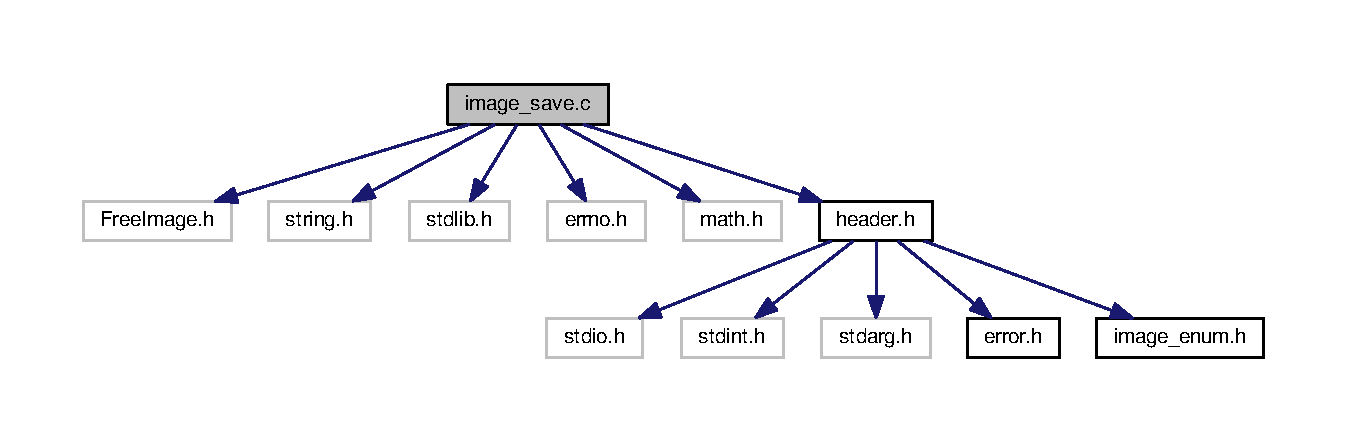
\includegraphics[width=350pt]{image__save_8c__incl}
\end{center}
\end{figure}
\subsection*{Functions}
\begin{DoxyCompactItemize}
\item 
\hyperlink{header_8h_a669b28ed18156f1a4f13732e070d6cf2}{bool} \hyperlink{image__save_8c_a3e561246e0ef24e90073c821f30d7c69}{imel\+\_\+image\+\_\+save\+\_\+ppm} (\hyperlink{header_8h_ad8298d38a89742ed84029b278c6acee5}{Imel\+Image} $\ast$image, const char $\ast$filename, \hyperlink{header_8h_abe31dcaa4b6683d315101c48b1ca2a56}{Imel\+Error} $\ast$error)
\begin{DoxyCompactList}\small\item\em Save image in P\+PM format. \end{DoxyCompactList}\item 
\hyperlink{header_8h_a669b28ed18156f1a4f13732e070d6cf2}{bool} \hyperlink{image__save_8c_a9c9b7dd3fca71a5060a44b131d511bae}{imel\+\_\+image\+\_\+save\+\_\+ppm\+\_\+handle} (\hyperlink{header_8h_ad8298d38a89742ed84029b278c6acee5}{Imel\+Image} $\ast$image, F\+I\+LE $\ast$of, \hyperlink{header_8h_abe31dcaa4b6683d315101c48b1ca2a56}{Imel\+Error} $\ast$error)
\begin{DoxyCompactList}\small\item\em Save image in P\+PM format in an already open file. \end{DoxyCompactList}\item 
\hyperlink{header_8h_a669b28ed18156f1a4f13732e070d6cf2}{bool} \hyperlink{image__save_8c_a5b84b5aa1c83a8fbf82d427113373f0e}{imel\+\_\+image\+\_\+save\+\_\+ppmraw} (\hyperlink{header_8h_ad8298d38a89742ed84029b278c6acee5}{Imel\+Image} $\ast$image, const char $\ast$filename, \hyperlink{header_8h_abe31dcaa4b6683d315101c48b1ca2a56}{Imel\+Error} $\ast$error)
\begin{DoxyCompactList}\small\item\em Save image in raw P\+PM format. \end{DoxyCompactList}\item 
\hyperlink{header_8h_a669b28ed18156f1a4f13732e070d6cf2}{bool} \hyperlink{image__save_8c_a4e5f415d7ce79245b8d96ab5c0abb8bf}{imel\+\_\+image\+\_\+save\+\_\+ppmraw\+\_\+handle} (\hyperlink{header_8h_ad8298d38a89742ed84029b278c6acee5}{Imel\+Image} $\ast$image, F\+I\+LE $\ast$of, \hyperlink{header_8h_abe31dcaa4b6683d315101c48b1ca2a56}{Imel\+Error} $\ast$error)
\begin{DoxyCompactList}\small\item\em Save image in raw P\+PM format in an already open file. \end{DoxyCompactList}\item 
\hyperlink{header_8h_a669b28ed18156f1a4f13732e070d6cf2}{bool} \hyperlink{image__save_8c_a7474441ad28c1bc48f104efe482218c9}{imel\+\_\+image\+\_\+save\+\_\+jpeg} (\hyperlink{header_8h_ad8298d38a89742ed84029b278c6acee5}{Imel\+Image} $\ast$image, const char $\ast$filename, int quality, \hyperlink{header_8h_abe31dcaa4b6683d315101c48b1ca2a56}{Imel\+Error} $\ast$error)
\begin{DoxyCompactList}\small\item\em Save image in J\+P\+EG format. \end{DoxyCompactList}\item 
\hyperlink{header_8h_a669b28ed18156f1a4f13732e070d6cf2}{bool} \hyperlink{image__save_8c_aecda64df0d3858bf33369c8ae7b92d87}{imel\+\_\+image\+\_\+save\+\_\+jpeg\+\_\+handle} (\hyperlink{header_8h_ad8298d38a89742ed84029b278c6acee5}{Imel\+Image} $\ast$image, F\+I\+LE $\ast$of, int quality, \hyperlink{header_8h_abe31dcaa4b6683d315101c48b1ca2a56}{Imel\+Error} $\ast$error)
\begin{DoxyCompactList}\small\item\em Save image in J\+P\+EG format in an already open file. \end{DoxyCompactList}\item 
\hyperlink{header_8h_a669b28ed18156f1a4f13732e070d6cf2}{bool} \hyperlink{image__save_8c_aa3e1e270563781e46013c98d05e952e7}{imel\+\_\+image\+\_\+save\+\_\+png} (\hyperlink{header_8h_ad8298d38a89742ed84029b278c6acee5}{Imel\+Image} $\ast$image, const char $\ast$filename, \hyperlink{image__enum_8h_a99c2986d48a651287d92e1f419f16a70}{Imel\+Png\+Flags} png\+\_\+flags, \hyperlink{header_8h_abe31dcaa4b6683d315101c48b1ca2a56}{Imel\+Error} $\ast$error)
\begin{DoxyCompactList}\small\item\em Save image in P\+NG format. \end{DoxyCompactList}\item 
\hyperlink{header_8h_a669b28ed18156f1a4f13732e070d6cf2}{bool} \hyperlink{image__save_8c_a727418390792881b6262e6392c476ba9}{imel\+\_\+image\+\_\+save\+\_\+png\+\_\+handle} (\hyperlink{header_8h_ad8298d38a89742ed84029b278c6acee5}{Imel\+Image} $\ast$image, F\+I\+LE $\ast$of, \hyperlink{image__enum_8h_a99c2986d48a651287d92e1f419f16a70}{Imel\+Png\+Flags} png\+\_\+flags, \hyperlink{header_8h_abe31dcaa4b6683d315101c48b1ca2a56}{Imel\+Error} $\ast$error)
\begin{DoxyCompactList}\small\item\em Save image in P\+NG format in an already open file. \end{DoxyCompactList}\item 
\hyperlink{header_8h_a669b28ed18156f1a4f13732e070d6cf2}{bool} \hyperlink{image__save_8c_afc28c02ce6aa3ae5fe765510603c51be}{imel\+\_\+image\+\_\+save\+\_\+tiff} (\hyperlink{header_8h_ad8298d38a89742ed84029b278c6acee5}{Imel\+Image} $\ast$image, const char $\ast$filename, \hyperlink{image__enum_8h_a519baf325b02bcca1d7eab10604c3a75}{Imel\+Tiff\+Flags} tiff\+\_\+flags, \hyperlink{header_8h_abe31dcaa4b6683d315101c48b1ca2a56}{Imel\+Error} $\ast$error)
\begin{DoxyCompactList}\small\item\em Save image in T\+I\+FF format. \end{DoxyCompactList}\item 
\hyperlink{header_8h_a669b28ed18156f1a4f13732e070d6cf2}{bool} \hyperlink{image__save_8c_a2e41ce825e969c57d1931fb58a05e920}{imel\+\_\+image\+\_\+save\+\_\+tiff\+\_\+handle} (\hyperlink{header_8h_ad8298d38a89742ed84029b278c6acee5}{Imel\+Image} $\ast$image, F\+I\+LE $\ast$of, \hyperlink{image__enum_8h_a519baf325b02bcca1d7eab10604c3a75}{Imel\+Tiff\+Flags} tiff\+\_\+flags, \hyperlink{header_8h_abe31dcaa4b6683d315101c48b1ca2a56}{Imel\+Error} $\ast$error)
\begin{DoxyCompactList}\small\item\em Save image in T\+I\+FF format in an already open file. \end{DoxyCompactList}\item 
\hyperlink{header_8h_a669b28ed18156f1a4f13732e070d6cf2}{bool} \hyperlink{image__save_8c_a1aa3d464b358dcdc9e493382fd54c487}{imel\+\_\+image\+\_\+save\+\_\+wbmp} (\hyperlink{header_8h_ad8298d38a89742ed84029b278c6acee5}{Imel\+Image} $\ast$image, const char $\ast$filename, \hyperlink{header_8h_abe31dcaa4b6683d315101c48b1ca2a56}{Imel\+Error} $\ast$error)
\begin{DoxyCompactList}\small\item\em Save image in W\+B\+MP format. \end{DoxyCompactList}\item 
\hyperlink{header_8h_a669b28ed18156f1a4f13732e070d6cf2}{bool} \hyperlink{image__save_8c_ade0967b6943819bf46d0ef70729e08a9}{imel\+\_\+image\+\_\+save\+\_\+wbmp\+\_\+handle} (\hyperlink{header_8h_ad8298d38a89742ed84029b278c6acee5}{Imel\+Image} $\ast$image, F\+I\+LE $\ast$of, \hyperlink{header_8h_abe31dcaa4b6683d315101c48b1ca2a56}{Imel\+Error} $\ast$error)
\begin{DoxyCompactList}\small\item\em Save image in W\+B\+MP format in an already open file. \end{DoxyCompactList}\item 
\hyperlink{header_8h_a669b28ed18156f1a4f13732e070d6cf2}{bool} \hyperlink{image__save_8c_a49c937b0bf49cbe0d16b1d99895a5a2c}{imel\+\_\+image\+\_\+save\+\_\+bmp} (\hyperlink{header_8h_ad8298d38a89742ed84029b278c6acee5}{Imel\+Image} $\ast$image, const char $\ast$filename, \hyperlink{image__enum_8h_acb527c56bb1574fab526fc3a56bf6467}{Imel\+Bmp\+Bits} bits\+\_\+per\+\_\+pixel, \hyperlink{header_8h_abe31dcaa4b6683d315101c48b1ca2a56}{Imel\+Error} $\ast$error)
\begin{DoxyCompactList}\small\item\em Save image in B\+MP format. \end{DoxyCompactList}\item 
\hyperlink{header_8h_a669b28ed18156f1a4f13732e070d6cf2}{bool} \hyperlink{image__save_8c_a5c16cf3bd82cedc0ef11698a138f48a2}{imel\+\_\+image\+\_\+save\+\_\+bmp\+\_\+handle} (\hyperlink{header_8h_ad8298d38a89742ed84029b278c6acee5}{Imel\+Image} $\ast$image, F\+I\+LE $\ast$of, \hyperlink{image__enum_8h_acb527c56bb1574fab526fc3a56bf6467}{Imel\+Bmp\+Bits} bits\+\_\+per\+\_\+pixel, \hyperlink{header_8h_abe31dcaa4b6683d315101c48b1ca2a56}{Imel\+Error} $\ast$error)
\begin{DoxyCompactList}\small\item\em Save image in B\+MP format in an already open file. \end{DoxyCompactList}\item 
\hyperlink{header_8h_a669b28ed18156f1a4f13732e070d6cf2}{bool} \hyperlink{image__save_8c_a5ae9a290272e18ad24a6ea9b54784048}{imel\+\_\+image\+\_\+save\+\_\+j2k} (\hyperlink{header_8h_ad8298d38a89742ed84029b278c6acee5}{Imel\+Image} $\ast$image, const char $\ast$filename, \hyperlink{image__enum_8h_a75c4f86d6bd9c093d99f5816f84da19d}{Imel\+J2k\+Bits} bits\+\_\+per\+\_\+pixel, \hyperlink{header_8h_abe31dcaa4b6683d315101c48b1ca2a56}{Imel\+Error} $\ast$error)
\begin{DoxyCompactList}\small\item\em Save image in J2K format. \end{DoxyCompactList}\item 
\hyperlink{header_8h_a669b28ed18156f1a4f13732e070d6cf2}{bool} \hyperlink{image__save_8c_afd3d307d7c5df250aa340dc54576ea12}{imel\+\_\+image\+\_\+save\+\_\+j2k\+\_\+handle} (\hyperlink{header_8h_ad8298d38a89742ed84029b278c6acee5}{Imel\+Image} $\ast$image, F\+I\+LE $\ast$of, \hyperlink{image__enum_8h_a75c4f86d6bd9c093d99f5816f84da19d}{Imel\+J2k\+Bits} bits\+\_\+per\+\_\+pixel, \hyperlink{header_8h_abe31dcaa4b6683d315101c48b1ca2a56}{Imel\+Error} $\ast$error)
\begin{DoxyCompactList}\small\item\em Save image in J2K format in an already open file. \end{DoxyCompactList}\item 
\hyperlink{header_8h_a669b28ed18156f1a4f13732e070d6cf2}{bool} \hyperlink{image__save_8c_aa1cdfb54662c2df3573cdca6de25ad63}{imel\+\_\+image\+\_\+save\+\_\+jp2} (\hyperlink{header_8h_ad8298d38a89742ed84029b278c6acee5}{Imel\+Image} $\ast$image, const char $\ast$filename, \hyperlink{image__enum_8h_a75c4f86d6bd9c093d99f5816f84da19d}{Imel\+J2k\+Bits} bits\+\_\+per\+\_\+pixel, \hyperlink{header_8h_abe31dcaa4b6683d315101c48b1ca2a56}{Imel\+Error} $\ast$error)
\begin{DoxyCompactList}\small\item\em Save image in J\+P2 format. \end{DoxyCompactList}\item 
\hyperlink{header_8h_a669b28ed18156f1a4f13732e070d6cf2}{bool} \hyperlink{image__save_8c_a70642f0e5d723ba1c46e8b7739d77d14}{imel\+\_\+image\+\_\+save\+\_\+jp2\+\_\+handle} (\hyperlink{header_8h_ad8298d38a89742ed84029b278c6acee5}{Imel\+Image} $\ast$image, F\+I\+LE $\ast$of, \hyperlink{image__enum_8h_a75c4f86d6bd9c093d99f5816f84da19d}{Imel\+J2k\+Bits} bits\+\_\+per\+\_\+pixel, \hyperlink{header_8h_abe31dcaa4b6683d315101c48b1ca2a56}{Imel\+Error} $\ast$error)
\begin{DoxyCompactList}\small\item\em Save image in J\+P2 format in an already open file. \end{DoxyCompactList}\item 
\hyperlink{header_8h_a669b28ed18156f1a4f13732e070d6cf2}{bool} \hyperlink{image__save_8c_a00621fb98f3614d2b53274c732099adb}{imel\+\_\+image\+\_\+save\+\_\+xpm} (\hyperlink{header_8h_ad8298d38a89742ed84029b278c6acee5}{Imel\+Image} $\ast$image, const char $\ast$filename, \hyperlink{header_8h_abe31dcaa4b6683d315101c48b1ca2a56}{Imel\+Error} $\ast$error)
\begin{DoxyCompactList}\small\item\em Save image in X\+PM format. \end{DoxyCompactList}\item 
\hyperlink{header_8h_a669b28ed18156f1a4f13732e070d6cf2}{bool} \hyperlink{image__save_8c_af8d4383ba5e386a6249f5955b88e0f91}{imel\+\_\+image\+\_\+save\+\_\+xpm\+\_\+handle} (\hyperlink{header_8h_ad8298d38a89742ed84029b278c6acee5}{Imel\+Image} $\ast$image, F\+I\+LE $\ast$of, \hyperlink{header_8h_abe31dcaa4b6683d315101c48b1ca2a56}{Imel\+Error} $\ast$error)
\begin{DoxyCompactList}\small\item\em Save image in X\+PM format in an already open file. \end{DoxyCompactList}\item 
\hyperlink{header_8h_a669b28ed18156f1a4f13732e070d6cf2}{bool} \hyperlink{image__save_8c_ac6a0d1b8734bd7692061c27ed46f00ca}{imel\+\_\+image\+\_\+save\+\_\+imel} (\hyperlink{header_8h_ad8298d38a89742ed84029b278c6acee5}{Imel\+Image} $\ast$image, const char $\ast$filename, \hyperlink{header_8h_abe31dcaa4b6683d315101c48b1ca2a56}{Imel\+Error} $\ast$error)
\begin{DoxyCompactList}\small\item\em Save image in I\+M\+EL format. \end{DoxyCompactList}\end{DoxyCompactItemize}


\subsection{Detailed Description}
This file contains function to save in different image format. 

\begin{DoxyAuthor}{Author}
Davide Francesco Merico 
\end{DoxyAuthor}


\subsection{Function Documentation}
\index{image\+\_\+save.\+c@{image\+\_\+save.\+c}!imel\+\_\+image\+\_\+save\+\_\+bmp@{imel\+\_\+image\+\_\+save\+\_\+bmp}}
\index{imel\+\_\+image\+\_\+save\+\_\+bmp@{imel\+\_\+image\+\_\+save\+\_\+bmp}!image\+\_\+save.\+c@{image\+\_\+save.\+c}}
\subsubsection[{\texorpdfstring{imel\+\_\+image\+\_\+save\+\_\+bmp(\+Imel\+Image $\ast$image, const char $\ast$filename, Imel\+Bmp\+Bits bits\+\_\+per\+\_\+pixel, Imel\+Error $\ast$error)}{imel_image_save_bmp(ImelImage *image, const char *filename, ImelBmpBits bits_per_pixel, ImelError *error)}}]{\setlength{\rightskip}{0pt plus 5cm}{\bf bool} imel\+\_\+image\+\_\+save\+\_\+bmp (
\begin{DoxyParamCaption}
\item[{{\bf Imel\+Image} $\ast$}]{image, }
\item[{const char $\ast$}]{filename, }
\item[{{\bf Imel\+Bmp\+Bits}}]{bits\+\_\+per\+\_\+pixel, }
\item[{{\bf Imel\+Error} $\ast$}]{error}
\end{DoxyParamCaption}
)}\hypertarget{image__save_8c_a49c937b0bf49cbe0d16b1d99895a5a2c}{}\label{image__save_8c_a49c937b0bf49cbe0d16b1d99895a5a2c}


Save image in B\+MP format. 


\begin{DoxyParams}{Parameters}
{\em image} & Image to save \\
\hline
{\em filename} & Output file name \\
\hline
{\em bits\+\_\+per\+\_\+pixel} & Save options \\
\hline
{\em error} & Error variable if you want handle the errors or N\+U\+LL. \\
\hline
\end{DoxyParams}
\begin{DoxyReturn}{Returns}
T\+R\+UE on success or F\+A\+L\+SE on error.
\end{DoxyReturn}
\begin{DoxySeeAlso}{See also}
\hyperlink{image__enum_8h_acb527c56bb1574fab526fc3a56bf6467}{Imel\+Bmp\+Bits} 

\hyperlink{image__save_8c_a5c16cf3bd82cedc0ef11698a138f48a2}{imel\+\_\+image\+\_\+save\+\_\+bmp\+\_\+handle} 
\end{DoxySeeAlso}
\index{image\+\_\+save.\+c@{image\+\_\+save.\+c}!imel\+\_\+image\+\_\+save\+\_\+bmp\+\_\+handle@{imel\+\_\+image\+\_\+save\+\_\+bmp\+\_\+handle}}
\index{imel\+\_\+image\+\_\+save\+\_\+bmp\+\_\+handle@{imel\+\_\+image\+\_\+save\+\_\+bmp\+\_\+handle}!image\+\_\+save.\+c@{image\+\_\+save.\+c}}
\subsubsection[{\texorpdfstring{imel\+\_\+image\+\_\+save\+\_\+bmp\+\_\+handle(\+Imel\+Image $\ast$image, F\+I\+L\+E $\ast$of, Imel\+Bmp\+Bits bits\+\_\+per\+\_\+pixel, Imel\+Error $\ast$error)}{imel_image_save_bmp_handle(ImelImage *image, FILE *of, ImelBmpBits bits_per_pixel, ImelError *error)}}]{\setlength{\rightskip}{0pt plus 5cm}{\bf bool} imel\+\_\+image\+\_\+save\+\_\+bmp\+\_\+handle (
\begin{DoxyParamCaption}
\item[{{\bf Imel\+Image} $\ast$}]{image, }
\item[{F\+I\+LE $\ast$}]{of, }
\item[{{\bf Imel\+Bmp\+Bits}}]{bits\+\_\+per\+\_\+pixel, }
\item[{{\bf Imel\+Error} $\ast$}]{error}
\end{DoxyParamCaption}
)}\hypertarget{image__save_8c_a5c16cf3bd82cedc0ef11698a138f48a2}{}\label{image__save_8c_a5c16cf3bd82cedc0ef11698a138f48a2}


Save image in B\+MP format in an already open file. 


\begin{DoxyParams}{Parameters}
{\em image} & Image to save \\
\hline
{\em of} & Output F\+I\+LE \\
\hline
{\em bits\+\_\+per\+\_\+pixel} & Save options \\
\hline
{\em error} & Error variable if you want handle the errors or N\+U\+LL. \\
\hline
\end{DoxyParams}
\begin{DoxyReturn}{Returns}
T\+R\+UE on success or F\+A\+L\+SE on error.
\end{DoxyReturn}
\begin{DoxySeeAlso}{See also}
\hyperlink{image__enum_8h_acb527c56bb1574fab526fc3a56bf6467}{Imel\+Bmp\+Bits} 

\hyperlink{image__save_8c_a49c937b0bf49cbe0d16b1d99895a5a2c}{imel\+\_\+image\+\_\+save\+\_\+bmp} 
\end{DoxySeeAlso}
\index{image\+\_\+save.\+c@{image\+\_\+save.\+c}!imel\+\_\+image\+\_\+save\+\_\+imel@{imel\+\_\+image\+\_\+save\+\_\+imel}}
\index{imel\+\_\+image\+\_\+save\+\_\+imel@{imel\+\_\+image\+\_\+save\+\_\+imel}!image\+\_\+save.\+c@{image\+\_\+save.\+c}}
\subsubsection[{\texorpdfstring{imel\+\_\+image\+\_\+save\+\_\+imel(\+Imel\+Image $\ast$image, const char $\ast$filename, Imel\+Error $\ast$error)}{imel_image_save_imel(ImelImage *image, const char *filename, ImelError *error)}}]{\setlength{\rightskip}{0pt plus 5cm}{\bf bool} imel\+\_\+image\+\_\+save\+\_\+imel (
\begin{DoxyParamCaption}
\item[{{\bf Imel\+Image} $\ast$}]{image, }
\item[{const char $\ast$}]{filename, }
\item[{{\bf Imel\+Error} $\ast$}]{error}
\end{DoxyParamCaption}
)}\hypertarget{image__save_8c_ac6a0d1b8734bd7692061c27ed46f00ca}{}\label{image__save_8c_ac6a0d1b8734bd7692061c27ed46f00ca}


Save image in I\+M\+EL format. 


\begin{DoxyParams}{Parameters}
{\em image} & Image to save \\
\hline
{\em filename} & Output file name \\
\hline
{\em error} & Error variable if you want handle the errors or N\+U\+LL. \\
\hline
\end{DoxyParams}
\begin{DoxyReturn}{Returns}
T\+R\+UE on success or F\+A\+L\+SE on error. 
\end{DoxyReturn}
\index{image\+\_\+save.\+c@{image\+\_\+save.\+c}!imel\+\_\+image\+\_\+save\+\_\+j2k@{imel\+\_\+image\+\_\+save\+\_\+j2k}}
\index{imel\+\_\+image\+\_\+save\+\_\+j2k@{imel\+\_\+image\+\_\+save\+\_\+j2k}!image\+\_\+save.\+c@{image\+\_\+save.\+c}}
\subsubsection[{\texorpdfstring{imel\+\_\+image\+\_\+save\+\_\+j2k(\+Imel\+Image $\ast$image, const char $\ast$filename, Imel\+J2k\+Bits bits\+\_\+per\+\_\+pixel, Imel\+Error $\ast$error)}{imel_image_save_j2k(ImelImage *image, const char *filename, ImelJ2kBits bits_per_pixel, ImelError *error)}}]{\setlength{\rightskip}{0pt plus 5cm}{\bf bool} imel\+\_\+image\+\_\+save\+\_\+j2k (
\begin{DoxyParamCaption}
\item[{{\bf Imel\+Image} $\ast$}]{image, }
\item[{const char $\ast$}]{filename, }
\item[{{\bf Imel\+J2k\+Bits}}]{bits\+\_\+per\+\_\+pixel, }
\item[{{\bf Imel\+Error} $\ast$}]{error}
\end{DoxyParamCaption}
)}\hypertarget{image__save_8c_a5ae9a290272e18ad24a6ea9b54784048}{}\label{image__save_8c_a5ae9a290272e18ad24a6ea9b54784048}


Save image in J2K format. 


\begin{DoxyParams}{Parameters}
{\em image} & Image to save \\
\hline
{\em filename} & Output file name \\
\hline
{\em bits\+\_\+per\+\_\+pixel} & Save options \\
\hline
{\em error} & Error variable if you want handle the errors or N\+U\+LL. \\
\hline
\end{DoxyParams}
\begin{DoxyReturn}{Returns}
T\+R\+UE on success or F\+A\+L\+SE on error.
\end{DoxyReturn}
\begin{DoxySeeAlso}{See also}
\hyperlink{image__enum_8h_a75c4f86d6bd9c093d99f5816f84da19d}{Imel\+J2k\+Bits} 

\hyperlink{image__save_8c_afd3d307d7c5df250aa340dc54576ea12}{imel\+\_\+image\+\_\+save\+\_\+j2k\+\_\+handle} 
\end{DoxySeeAlso}
\index{image\+\_\+save.\+c@{image\+\_\+save.\+c}!imel\+\_\+image\+\_\+save\+\_\+j2k\+\_\+handle@{imel\+\_\+image\+\_\+save\+\_\+j2k\+\_\+handle}}
\index{imel\+\_\+image\+\_\+save\+\_\+j2k\+\_\+handle@{imel\+\_\+image\+\_\+save\+\_\+j2k\+\_\+handle}!image\+\_\+save.\+c@{image\+\_\+save.\+c}}
\subsubsection[{\texorpdfstring{imel\+\_\+image\+\_\+save\+\_\+j2k\+\_\+handle(\+Imel\+Image $\ast$image, F\+I\+L\+E $\ast$of, Imel\+J2k\+Bits bits\+\_\+per\+\_\+pixel, Imel\+Error $\ast$error)}{imel_image_save_j2k_handle(ImelImage *image, FILE *of, ImelJ2kBits bits_per_pixel, ImelError *error)}}]{\setlength{\rightskip}{0pt plus 5cm}{\bf bool} imel\+\_\+image\+\_\+save\+\_\+j2k\+\_\+handle (
\begin{DoxyParamCaption}
\item[{{\bf Imel\+Image} $\ast$}]{image, }
\item[{F\+I\+LE $\ast$}]{of, }
\item[{{\bf Imel\+J2k\+Bits}}]{bits\+\_\+per\+\_\+pixel, }
\item[{{\bf Imel\+Error} $\ast$}]{error}
\end{DoxyParamCaption}
)}\hypertarget{image__save_8c_afd3d307d7c5df250aa340dc54576ea12}{}\label{image__save_8c_afd3d307d7c5df250aa340dc54576ea12}


Save image in J2K format in an already open file. 


\begin{DoxyParams}{Parameters}
{\em image} & Image to save \\
\hline
{\em of} & Output F\+I\+LE \\
\hline
{\em bits\+\_\+per\+\_\+pixel} & Save options \\
\hline
{\em error} & Error variable if you want handle the errors or N\+U\+LL. \\
\hline
\end{DoxyParams}
\begin{DoxyReturn}{Returns}
T\+R\+UE on success or F\+A\+L\+SE on error.
\end{DoxyReturn}
\begin{DoxySeeAlso}{See also}
\hyperlink{image__enum_8h_a75c4f86d6bd9c093d99f5816f84da19d}{Imel\+J2k\+Bits} 

\hyperlink{image__save_8c_a5ae9a290272e18ad24a6ea9b54784048}{imel\+\_\+image\+\_\+save\+\_\+j2k} 
\end{DoxySeeAlso}
\index{image\+\_\+save.\+c@{image\+\_\+save.\+c}!imel\+\_\+image\+\_\+save\+\_\+jp2@{imel\+\_\+image\+\_\+save\+\_\+jp2}}
\index{imel\+\_\+image\+\_\+save\+\_\+jp2@{imel\+\_\+image\+\_\+save\+\_\+jp2}!image\+\_\+save.\+c@{image\+\_\+save.\+c}}
\subsubsection[{\texorpdfstring{imel\+\_\+image\+\_\+save\+\_\+jp2(\+Imel\+Image $\ast$image, const char $\ast$filename, Imel\+J2k\+Bits bits\+\_\+per\+\_\+pixel, Imel\+Error $\ast$error)}{imel_image_save_jp2(ImelImage *image, const char *filename, ImelJ2kBits bits_per_pixel, ImelError *error)}}]{\setlength{\rightskip}{0pt plus 5cm}{\bf bool} imel\+\_\+image\+\_\+save\+\_\+jp2 (
\begin{DoxyParamCaption}
\item[{{\bf Imel\+Image} $\ast$}]{image, }
\item[{const char $\ast$}]{filename, }
\item[{{\bf Imel\+J2k\+Bits}}]{bits\+\_\+per\+\_\+pixel, }
\item[{{\bf Imel\+Error} $\ast$}]{error}
\end{DoxyParamCaption}
)}\hypertarget{image__save_8c_aa1cdfb54662c2df3573cdca6de25ad63}{}\label{image__save_8c_aa1cdfb54662c2df3573cdca6de25ad63}


Save image in J\+P2 format. 


\begin{DoxyParams}{Parameters}
{\em image} & Image to save \\
\hline
{\em filename} & Output file name \\
\hline
{\em bits\+\_\+per\+\_\+pixel} & Save options \\
\hline
{\em error} & Error variable if you want handle the errors or N\+U\+LL. \\
\hline
\end{DoxyParams}
\begin{DoxyReturn}{Returns}
T\+R\+UE on success or F\+A\+L\+SE on error.
\end{DoxyReturn}
\begin{DoxySeeAlso}{See also}
\hyperlink{image__enum_8h_a75c4f86d6bd9c093d99f5816f84da19d}{Imel\+J2k\+Bits} 

\hyperlink{image__save_8c_a70642f0e5d723ba1c46e8b7739d77d14}{imel\+\_\+image\+\_\+save\+\_\+jp2\+\_\+handle} 
\end{DoxySeeAlso}
\index{image\+\_\+save.\+c@{image\+\_\+save.\+c}!imel\+\_\+image\+\_\+save\+\_\+jp2\+\_\+handle@{imel\+\_\+image\+\_\+save\+\_\+jp2\+\_\+handle}}
\index{imel\+\_\+image\+\_\+save\+\_\+jp2\+\_\+handle@{imel\+\_\+image\+\_\+save\+\_\+jp2\+\_\+handle}!image\+\_\+save.\+c@{image\+\_\+save.\+c}}
\subsubsection[{\texorpdfstring{imel\+\_\+image\+\_\+save\+\_\+jp2\+\_\+handle(\+Imel\+Image $\ast$image, F\+I\+L\+E $\ast$of, Imel\+J2k\+Bits bits\+\_\+per\+\_\+pixel, Imel\+Error $\ast$error)}{imel_image_save_jp2_handle(ImelImage *image, FILE *of, ImelJ2kBits bits_per_pixel, ImelError *error)}}]{\setlength{\rightskip}{0pt plus 5cm}{\bf bool} imel\+\_\+image\+\_\+save\+\_\+jp2\+\_\+handle (
\begin{DoxyParamCaption}
\item[{{\bf Imel\+Image} $\ast$}]{image, }
\item[{F\+I\+LE $\ast$}]{of, }
\item[{{\bf Imel\+J2k\+Bits}}]{bits\+\_\+per\+\_\+pixel, }
\item[{{\bf Imel\+Error} $\ast$}]{error}
\end{DoxyParamCaption}
)}\hypertarget{image__save_8c_a70642f0e5d723ba1c46e8b7739d77d14}{}\label{image__save_8c_a70642f0e5d723ba1c46e8b7739d77d14}


Save image in J\+P2 format in an already open file. 


\begin{DoxyParams}{Parameters}
{\em image} & Image to save \\
\hline
{\em of} & Output F\+I\+LE \\
\hline
{\em bits\+\_\+per\+\_\+pixel} & Save options \\
\hline
{\em error} & Error variable if you want handle the errors or N\+U\+LL. \\
\hline
\end{DoxyParams}
\begin{DoxyReturn}{Returns}
T\+R\+UE on success or F\+A\+L\+SE on error.
\end{DoxyReturn}
\begin{DoxySeeAlso}{See also}
\hyperlink{image__enum_8h_a75c4f86d6bd9c093d99f5816f84da19d}{Imel\+J2k\+Bits} 

\hyperlink{image__save_8c_aa1cdfb54662c2df3573cdca6de25ad63}{imel\+\_\+image\+\_\+save\+\_\+jp2} 
\end{DoxySeeAlso}
\index{image\+\_\+save.\+c@{image\+\_\+save.\+c}!imel\+\_\+image\+\_\+save\+\_\+jpeg@{imel\+\_\+image\+\_\+save\+\_\+jpeg}}
\index{imel\+\_\+image\+\_\+save\+\_\+jpeg@{imel\+\_\+image\+\_\+save\+\_\+jpeg}!image\+\_\+save.\+c@{image\+\_\+save.\+c}}
\subsubsection[{\texorpdfstring{imel\+\_\+image\+\_\+save\+\_\+jpeg(\+Imel\+Image $\ast$image, const char $\ast$filename, int quality, Imel\+Error $\ast$error)}{imel_image_save_jpeg(ImelImage *image, const char *filename, int quality, ImelError *error)}}]{\setlength{\rightskip}{0pt plus 5cm}{\bf bool} imel\+\_\+image\+\_\+save\+\_\+jpeg (
\begin{DoxyParamCaption}
\item[{{\bf Imel\+Image} $\ast$}]{image, }
\item[{const char $\ast$}]{filename, }
\item[{int}]{quality, }
\item[{{\bf Imel\+Error} $\ast$}]{error}
\end{DoxyParamCaption}
)}\hypertarget{image__save_8c_a7474441ad28c1bc48f104efe482218c9}{}\label{image__save_8c_a7474441ad28c1bc48f104efe482218c9}


Save image in J\+P\+EG format. 


\begin{DoxyParams}{Parameters}
{\em image} & Image to save \\
\hline
{\em filename} & Output file name \\
\hline
{\em quality} & Save quality. Values between 0 and 100. \\
\hline
{\em error} & Error variable if you want handle the errors or N\+U\+LL. \\
\hline
\end{DoxyParams}
\begin{DoxyReturn}{Returns}
T\+R\+UE on success or F\+A\+L\+SE on error.
\end{DoxyReturn}
\begin{DoxySeeAlso}{See also}
\hyperlink{image__save_8c_aecda64df0d3858bf33369c8ae7b92d87}{imel\+\_\+image\+\_\+save\+\_\+jpeg\+\_\+handle} 
\end{DoxySeeAlso}
\index{image\+\_\+save.\+c@{image\+\_\+save.\+c}!imel\+\_\+image\+\_\+save\+\_\+jpeg\+\_\+handle@{imel\+\_\+image\+\_\+save\+\_\+jpeg\+\_\+handle}}
\index{imel\+\_\+image\+\_\+save\+\_\+jpeg\+\_\+handle@{imel\+\_\+image\+\_\+save\+\_\+jpeg\+\_\+handle}!image\+\_\+save.\+c@{image\+\_\+save.\+c}}
\subsubsection[{\texorpdfstring{imel\+\_\+image\+\_\+save\+\_\+jpeg\+\_\+handle(\+Imel\+Image $\ast$image, F\+I\+L\+E $\ast$of, int quality, Imel\+Error $\ast$error)}{imel_image_save_jpeg_handle(ImelImage *image, FILE *of, int quality, ImelError *error)}}]{\setlength{\rightskip}{0pt plus 5cm}{\bf bool} imel\+\_\+image\+\_\+save\+\_\+jpeg\+\_\+handle (
\begin{DoxyParamCaption}
\item[{{\bf Imel\+Image} $\ast$}]{image, }
\item[{F\+I\+LE $\ast$}]{of, }
\item[{int}]{quality, }
\item[{{\bf Imel\+Error} $\ast$}]{error}
\end{DoxyParamCaption}
)}\hypertarget{image__save_8c_aecda64df0d3858bf33369c8ae7b92d87}{}\label{image__save_8c_aecda64df0d3858bf33369c8ae7b92d87}


Save image in J\+P\+EG format in an already open file. 


\begin{DoxyParams}{Parameters}
{\em image} & Image to save \\
\hline
{\em of} & Output F\+I\+LE \\
\hline
{\em quality} & Save quality. Values between 0 and 100. \\
\hline
{\em error} & Error variable if you want handle the errors or N\+U\+LL. \\
\hline
\end{DoxyParams}
\begin{DoxyReturn}{Returns}
T\+R\+UE on success or F\+A\+L\+SE on error.
\end{DoxyReturn}
\begin{DoxySeeAlso}{See also}
\hyperlink{image__save_8c_a7474441ad28c1bc48f104efe482218c9}{imel\+\_\+image\+\_\+save\+\_\+jpeg} 
\end{DoxySeeAlso}
\index{image\+\_\+save.\+c@{image\+\_\+save.\+c}!imel\+\_\+image\+\_\+save\+\_\+png@{imel\+\_\+image\+\_\+save\+\_\+png}}
\index{imel\+\_\+image\+\_\+save\+\_\+png@{imel\+\_\+image\+\_\+save\+\_\+png}!image\+\_\+save.\+c@{image\+\_\+save.\+c}}
\subsubsection[{\texorpdfstring{imel\+\_\+image\+\_\+save\+\_\+png(\+Imel\+Image $\ast$image, const char $\ast$filename, Imel\+Png\+Flags png\+\_\+flags, Imel\+Error $\ast$error)}{imel_image_save_png(ImelImage *image, const char *filename, ImelPngFlags png_flags, ImelError *error)}}]{\setlength{\rightskip}{0pt plus 5cm}{\bf bool} imel\+\_\+image\+\_\+save\+\_\+png (
\begin{DoxyParamCaption}
\item[{{\bf Imel\+Image} $\ast$}]{image, }
\item[{const char $\ast$}]{filename, }
\item[{{\bf Imel\+Png\+Flags}}]{png\+\_\+flags, }
\item[{{\bf Imel\+Error} $\ast$}]{error}
\end{DoxyParamCaption}
)}\hypertarget{image__save_8c_aa3e1e270563781e46013c98d05e952e7}{}\label{image__save_8c_aa3e1e270563781e46013c98d05e952e7}


Save image in P\+NG format. 


\begin{DoxyParams}{Parameters}
{\em image} & Image to save \\
\hline
{\em filename} & Output file name \\
\hline
{\em png\+\_\+flags} & Save options \\
\hline
{\em error} & Error variable if you want handle the errors or N\+U\+LL. \\
\hline
\end{DoxyParams}
\begin{DoxyReturn}{Returns}
T\+R\+UE on success or F\+A\+L\+SE on error.
\end{DoxyReturn}
\begin{DoxySeeAlso}{See also}
\hyperlink{image__enum_8h_a99c2986d48a651287d92e1f419f16a70}{Imel\+Png\+Flags} 

\hyperlink{image__save_8c_a727418390792881b6262e6392c476ba9}{imel\+\_\+image\+\_\+save\+\_\+png\+\_\+handle} 
\end{DoxySeeAlso}
\index{image\+\_\+save.\+c@{image\+\_\+save.\+c}!imel\+\_\+image\+\_\+save\+\_\+png\+\_\+handle@{imel\+\_\+image\+\_\+save\+\_\+png\+\_\+handle}}
\index{imel\+\_\+image\+\_\+save\+\_\+png\+\_\+handle@{imel\+\_\+image\+\_\+save\+\_\+png\+\_\+handle}!image\+\_\+save.\+c@{image\+\_\+save.\+c}}
\subsubsection[{\texorpdfstring{imel\+\_\+image\+\_\+save\+\_\+png\+\_\+handle(\+Imel\+Image $\ast$image, F\+I\+L\+E $\ast$of, Imel\+Png\+Flags png\+\_\+flags, Imel\+Error $\ast$error)}{imel_image_save_png_handle(ImelImage *image, FILE *of, ImelPngFlags png_flags, ImelError *error)}}]{\setlength{\rightskip}{0pt plus 5cm}{\bf bool} imel\+\_\+image\+\_\+save\+\_\+png\+\_\+handle (
\begin{DoxyParamCaption}
\item[{{\bf Imel\+Image} $\ast$}]{image, }
\item[{F\+I\+LE $\ast$}]{of, }
\item[{{\bf Imel\+Png\+Flags}}]{png\+\_\+flags, }
\item[{{\bf Imel\+Error} $\ast$}]{error}
\end{DoxyParamCaption}
)}\hypertarget{image__save_8c_a727418390792881b6262e6392c476ba9}{}\label{image__save_8c_a727418390792881b6262e6392c476ba9}


Save image in P\+NG format in an already open file. 


\begin{DoxyParams}{Parameters}
{\em image} & Image to save \\
\hline
{\em of} & Output F\+I\+LE \\
\hline
{\em png\+\_\+flags} & Save options \\
\hline
{\em error} & Error variable if you want handle the errors or N\+U\+LL. \\
\hline
\end{DoxyParams}
\begin{DoxyReturn}{Returns}
T\+R\+UE on success or F\+A\+L\+SE on error.
\end{DoxyReturn}
\begin{DoxySeeAlso}{See also}
\hyperlink{image__enum_8h_a99c2986d48a651287d92e1f419f16a70}{Imel\+Png\+Flags} 

\hyperlink{image__save_8c_aa3e1e270563781e46013c98d05e952e7}{imel\+\_\+image\+\_\+save\+\_\+png} 
\end{DoxySeeAlso}
\index{image\+\_\+save.\+c@{image\+\_\+save.\+c}!imel\+\_\+image\+\_\+save\+\_\+ppm@{imel\+\_\+image\+\_\+save\+\_\+ppm}}
\index{imel\+\_\+image\+\_\+save\+\_\+ppm@{imel\+\_\+image\+\_\+save\+\_\+ppm}!image\+\_\+save.\+c@{image\+\_\+save.\+c}}
\subsubsection[{\texorpdfstring{imel\+\_\+image\+\_\+save\+\_\+ppm(\+Imel\+Image $\ast$image, const char $\ast$filename, Imel\+Error $\ast$error)}{imel_image_save_ppm(ImelImage *image, const char *filename, ImelError *error)}}]{\setlength{\rightskip}{0pt plus 5cm}{\bf bool} imel\+\_\+image\+\_\+save\+\_\+ppm (
\begin{DoxyParamCaption}
\item[{{\bf Imel\+Image} $\ast$}]{image, }
\item[{const char $\ast$}]{filename, }
\item[{{\bf Imel\+Error} $\ast$}]{error}
\end{DoxyParamCaption}
)}\hypertarget{image__save_8c_a3e561246e0ef24e90073c821f30d7c69}{}\label{image__save_8c_a3e561246e0ef24e90073c821f30d7c69}


Save image in P\+PM format. 


\begin{DoxyParams}{Parameters}
{\em image} & Image to save \\
\hline
{\em filename} & Output file name \\
\hline
{\em error} & Error variable if you want handle the errors or N\+U\+LL. \\
\hline
\end{DoxyParams}
\begin{DoxyReturn}{Returns}
T\+R\+UE on success or F\+A\+L\+SE on error.
\end{DoxyReturn}
\begin{DoxySeeAlso}{See also}
\hyperlink{image__save_8c_a9c9b7dd3fca71a5060a44b131d511bae}{imel\+\_\+image\+\_\+save\+\_\+ppm\+\_\+handle} 
\end{DoxySeeAlso}
\index{image\+\_\+save.\+c@{image\+\_\+save.\+c}!imel\+\_\+image\+\_\+save\+\_\+ppm\+\_\+handle@{imel\+\_\+image\+\_\+save\+\_\+ppm\+\_\+handle}}
\index{imel\+\_\+image\+\_\+save\+\_\+ppm\+\_\+handle@{imel\+\_\+image\+\_\+save\+\_\+ppm\+\_\+handle}!image\+\_\+save.\+c@{image\+\_\+save.\+c}}
\subsubsection[{\texorpdfstring{imel\+\_\+image\+\_\+save\+\_\+ppm\+\_\+handle(\+Imel\+Image $\ast$image, F\+I\+L\+E $\ast$of, Imel\+Error $\ast$error)}{imel_image_save_ppm_handle(ImelImage *image, FILE *of, ImelError *error)}}]{\setlength{\rightskip}{0pt plus 5cm}{\bf bool} imel\+\_\+image\+\_\+save\+\_\+ppm\+\_\+handle (
\begin{DoxyParamCaption}
\item[{{\bf Imel\+Image} $\ast$}]{image, }
\item[{F\+I\+LE $\ast$}]{of, }
\item[{{\bf Imel\+Error} $\ast$}]{error}
\end{DoxyParamCaption}
)}\hypertarget{image__save_8c_a9c9b7dd3fca71a5060a44b131d511bae}{}\label{image__save_8c_a9c9b7dd3fca71a5060a44b131d511bae}


Save image in P\+PM format in an already open file. 


\begin{DoxyParams}{Parameters}
{\em image} & Image to save \\
\hline
{\em of} & Output F\+I\+LE \\
\hline
{\em error} & Error variable if you want handle the errors or N\+U\+LL. \\
\hline
\end{DoxyParams}
\begin{DoxyReturn}{Returns}
T\+R\+UE on success or F\+A\+L\+SE on error.
\end{DoxyReturn}
\begin{DoxySeeAlso}{See also}
\hyperlink{image__save_8c_a3e561246e0ef24e90073c821f30d7c69}{imel\+\_\+image\+\_\+save\+\_\+ppm} 
\end{DoxySeeAlso}
\index{image\+\_\+save.\+c@{image\+\_\+save.\+c}!imel\+\_\+image\+\_\+save\+\_\+ppmraw@{imel\+\_\+image\+\_\+save\+\_\+ppmraw}}
\index{imel\+\_\+image\+\_\+save\+\_\+ppmraw@{imel\+\_\+image\+\_\+save\+\_\+ppmraw}!image\+\_\+save.\+c@{image\+\_\+save.\+c}}
\subsubsection[{\texorpdfstring{imel\+\_\+image\+\_\+save\+\_\+ppmraw(\+Imel\+Image $\ast$image, const char $\ast$filename, Imel\+Error $\ast$error)}{imel_image_save_ppmraw(ImelImage *image, const char *filename, ImelError *error)}}]{\setlength{\rightskip}{0pt plus 5cm}{\bf bool} imel\+\_\+image\+\_\+save\+\_\+ppmraw (
\begin{DoxyParamCaption}
\item[{{\bf Imel\+Image} $\ast$}]{image, }
\item[{const char $\ast$}]{filename, }
\item[{{\bf Imel\+Error} $\ast$}]{error}
\end{DoxyParamCaption}
)}\hypertarget{image__save_8c_a5b84b5aa1c83a8fbf82d427113373f0e}{}\label{image__save_8c_a5b84b5aa1c83a8fbf82d427113373f0e}


Save image in raw P\+PM format. 


\begin{DoxyParams}{Parameters}
{\em image} & Image to save \\
\hline
{\em filename} & Output file name \\
\hline
{\em error} & Error variable if you want handle the errors or N\+U\+LL. \\
\hline
\end{DoxyParams}
\begin{DoxyReturn}{Returns}
T\+R\+UE on success or F\+A\+L\+SE on error.
\end{DoxyReturn}
\begin{DoxySeeAlso}{See also}
\hyperlink{image__save_8c_a4e5f415d7ce79245b8d96ab5c0abb8bf}{imel\+\_\+image\+\_\+save\+\_\+ppmraw\+\_\+handle} 
\end{DoxySeeAlso}
\index{image\+\_\+save.\+c@{image\+\_\+save.\+c}!imel\+\_\+image\+\_\+save\+\_\+ppmraw\+\_\+handle@{imel\+\_\+image\+\_\+save\+\_\+ppmraw\+\_\+handle}}
\index{imel\+\_\+image\+\_\+save\+\_\+ppmraw\+\_\+handle@{imel\+\_\+image\+\_\+save\+\_\+ppmraw\+\_\+handle}!image\+\_\+save.\+c@{image\+\_\+save.\+c}}
\subsubsection[{\texorpdfstring{imel\+\_\+image\+\_\+save\+\_\+ppmraw\+\_\+handle(\+Imel\+Image $\ast$image, F\+I\+L\+E $\ast$of, Imel\+Error $\ast$error)}{imel_image_save_ppmraw_handle(ImelImage *image, FILE *of, ImelError *error)}}]{\setlength{\rightskip}{0pt plus 5cm}{\bf bool} imel\+\_\+image\+\_\+save\+\_\+ppmraw\+\_\+handle (
\begin{DoxyParamCaption}
\item[{{\bf Imel\+Image} $\ast$}]{image, }
\item[{F\+I\+LE $\ast$}]{of, }
\item[{{\bf Imel\+Error} $\ast$}]{error}
\end{DoxyParamCaption}
)}\hypertarget{image__save_8c_a4e5f415d7ce79245b8d96ab5c0abb8bf}{}\label{image__save_8c_a4e5f415d7ce79245b8d96ab5c0abb8bf}


Save image in raw P\+PM format in an already open file. 


\begin{DoxyParams}{Parameters}
{\em image} & Image to save \\
\hline
{\em of} & Output F\+I\+LE \\
\hline
{\em error} & Error variable if you want handle the errors or N\+U\+LL. \\
\hline
\end{DoxyParams}
\begin{DoxyReturn}{Returns}
T\+R\+UE on success or F\+A\+L\+SE on error.
\end{DoxyReturn}
\begin{DoxySeeAlso}{See also}
\hyperlink{image__save_8c_a5b84b5aa1c83a8fbf82d427113373f0e}{imel\+\_\+image\+\_\+save\+\_\+ppmraw} 
\end{DoxySeeAlso}
\index{image\+\_\+save.\+c@{image\+\_\+save.\+c}!imel\+\_\+image\+\_\+save\+\_\+tiff@{imel\+\_\+image\+\_\+save\+\_\+tiff}}
\index{imel\+\_\+image\+\_\+save\+\_\+tiff@{imel\+\_\+image\+\_\+save\+\_\+tiff}!image\+\_\+save.\+c@{image\+\_\+save.\+c}}
\subsubsection[{\texorpdfstring{imel\+\_\+image\+\_\+save\+\_\+tiff(\+Imel\+Image $\ast$image, const char $\ast$filename, Imel\+Tiff\+Flags tiff\+\_\+flags, Imel\+Error $\ast$error)}{imel_image_save_tiff(ImelImage *image, const char *filename, ImelTiffFlags tiff_flags, ImelError *error)}}]{\setlength{\rightskip}{0pt plus 5cm}{\bf bool} imel\+\_\+image\+\_\+save\+\_\+tiff (
\begin{DoxyParamCaption}
\item[{{\bf Imel\+Image} $\ast$}]{image, }
\item[{const char $\ast$}]{filename, }
\item[{{\bf Imel\+Tiff\+Flags}}]{tiff\+\_\+flags, }
\item[{{\bf Imel\+Error} $\ast$}]{error}
\end{DoxyParamCaption}
)}\hypertarget{image__save_8c_afc28c02ce6aa3ae5fe765510603c51be}{}\label{image__save_8c_afc28c02ce6aa3ae5fe765510603c51be}


Save image in T\+I\+FF format. 


\begin{DoxyParams}{Parameters}
{\em image} & Image to save \\
\hline
{\em filename} & Output file name \\
\hline
{\em tiff\+\_\+flags} & Save options \\
\hline
{\em error} & Error variable if you want handle the errors or N\+U\+LL. \\
\hline
\end{DoxyParams}
\begin{DoxyReturn}{Returns}
T\+R\+UE on success or F\+A\+L\+SE on error.
\end{DoxyReturn}
\begin{DoxySeeAlso}{See also}
\hyperlink{image__enum_8h_a519baf325b02bcca1d7eab10604c3a75}{Imel\+Tiff\+Flags} 

\hyperlink{image__save_8c_a2e41ce825e969c57d1931fb58a05e920}{imel\+\_\+image\+\_\+save\+\_\+tiff\+\_\+handle} 
\end{DoxySeeAlso}
\index{image\+\_\+save.\+c@{image\+\_\+save.\+c}!imel\+\_\+image\+\_\+save\+\_\+tiff\+\_\+handle@{imel\+\_\+image\+\_\+save\+\_\+tiff\+\_\+handle}}
\index{imel\+\_\+image\+\_\+save\+\_\+tiff\+\_\+handle@{imel\+\_\+image\+\_\+save\+\_\+tiff\+\_\+handle}!image\+\_\+save.\+c@{image\+\_\+save.\+c}}
\subsubsection[{\texorpdfstring{imel\+\_\+image\+\_\+save\+\_\+tiff\+\_\+handle(\+Imel\+Image $\ast$image, F\+I\+L\+E $\ast$of, Imel\+Tiff\+Flags tiff\+\_\+flags, Imel\+Error $\ast$error)}{imel_image_save_tiff_handle(ImelImage *image, FILE *of, ImelTiffFlags tiff_flags, ImelError *error)}}]{\setlength{\rightskip}{0pt plus 5cm}{\bf bool} imel\+\_\+image\+\_\+save\+\_\+tiff\+\_\+handle (
\begin{DoxyParamCaption}
\item[{{\bf Imel\+Image} $\ast$}]{image, }
\item[{F\+I\+LE $\ast$}]{of, }
\item[{{\bf Imel\+Tiff\+Flags}}]{tiff\+\_\+flags, }
\item[{{\bf Imel\+Error} $\ast$}]{error}
\end{DoxyParamCaption}
)}\hypertarget{image__save_8c_a2e41ce825e969c57d1931fb58a05e920}{}\label{image__save_8c_a2e41ce825e969c57d1931fb58a05e920}


Save image in T\+I\+FF format in an already open file. 


\begin{DoxyParams}{Parameters}
{\em image} & Image to save \\
\hline
{\em of} & Output F\+I\+LE \\
\hline
{\em tiff\+\_\+flags} & Save options \\
\hline
{\em error} & Error variable if you want handle the errors or N\+U\+LL. \\
\hline
\end{DoxyParams}
\begin{DoxyReturn}{Returns}
T\+R\+UE on success or F\+A\+L\+SE on error.
\end{DoxyReturn}
\begin{DoxySeeAlso}{See also}
\hyperlink{image__enum_8h_a519baf325b02bcca1d7eab10604c3a75}{Imel\+Tiff\+Flags} 

\hyperlink{image__save_8c_afc28c02ce6aa3ae5fe765510603c51be}{imel\+\_\+image\+\_\+save\+\_\+tiff} 
\end{DoxySeeAlso}
\index{image\+\_\+save.\+c@{image\+\_\+save.\+c}!imel\+\_\+image\+\_\+save\+\_\+wbmp@{imel\+\_\+image\+\_\+save\+\_\+wbmp}}
\index{imel\+\_\+image\+\_\+save\+\_\+wbmp@{imel\+\_\+image\+\_\+save\+\_\+wbmp}!image\+\_\+save.\+c@{image\+\_\+save.\+c}}
\subsubsection[{\texorpdfstring{imel\+\_\+image\+\_\+save\+\_\+wbmp(\+Imel\+Image $\ast$image, const char $\ast$filename, Imel\+Error $\ast$error)}{imel_image_save_wbmp(ImelImage *image, const char *filename, ImelError *error)}}]{\setlength{\rightskip}{0pt plus 5cm}{\bf bool} imel\+\_\+image\+\_\+save\+\_\+wbmp (
\begin{DoxyParamCaption}
\item[{{\bf Imel\+Image} $\ast$}]{image, }
\item[{const char $\ast$}]{filename, }
\item[{{\bf Imel\+Error} $\ast$}]{error}
\end{DoxyParamCaption}
)}\hypertarget{image__save_8c_a1aa3d464b358dcdc9e493382fd54c487}{}\label{image__save_8c_a1aa3d464b358dcdc9e493382fd54c487}


Save image in W\+B\+MP format. 


\begin{DoxyParams}{Parameters}
{\em image} & Image to save \\
\hline
{\em filename} & Output file name \\
\hline
{\em error} & Error variable if you want handle the errors or N\+U\+LL. \\
\hline
\end{DoxyParams}
\begin{DoxyReturn}{Returns}
T\+R\+UE on success or F\+A\+L\+SE on error.
\end{DoxyReturn}
\begin{DoxySeeAlso}{See also}
\hyperlink{image__save_8c_ade0967b6943819bf46d0ef70729e08a9}{imel\+\_\+image\+\_\+save\+\_\+wbmp\+\_\+handle} 
\end{DoxySeeAlso}
\index{image\+\_\+save.\+c@{image\+\_\+save.\+c}!imel\+\_\+image\+\_\+save\+\_\+wbmp\+\_\+handle@{imel\+\_\+image\+\_\+save\+\_\+wbmp\+\_\+handle}}
\index{imel\+\_\+image\+\_\+save\+\_\+wbmp\+\_\+handle@{imel\+\_\+image\+\_\+save\+\_\+wbmp\+\_\+handle}!image\+\_\+save.\+c@{image\+\_\+save.\+c}}
\subsubsection[{\texorpdfstring{imel\+\_\+image\+\_\+save\+\_\+wbmp\+\_\+handle(\+Imel\+Image $\ast$image, F\+I\+L\+E $\ast$of, Imel\+Error $\ast$error)}{imel_image_save_wbmp_handle(ImelImage *image, FILE *of, ImelError *error)}}]{\setlength{\rightskip}{0pt plus 5cm}{\bf bool} imel\+\_\+image\+\_\+save\+\_\+wbmp\+\_\+handle (
\begin{DoxyParamCaption}
\item[{{\bf Imel\+Image} $\ast$}]{image, }
\item[{F\+I\+LE $\ast$}]{of, }
\item[{{\bf Imel\+Error} $\ast$}]{error}
\end{DoxyParamCaption}
)}\hypertarget{image__save_8c_ade0967b6943819bf46d0ef70729e08a9}{}\label{image__save_8c_ade0967b6943819bf46d0ef70729e08a9}


Save image in W\+B\+MP format in an already open file. 


\begin{DoxyParams}{Parameters}
{\em image} & Image to save \\
\hline
{\em of} & Output F\+I\+LE \\
\hline
{\em error} & Error variable if you want handle the errors or N\+U\+LL. \\
\hline
\end{DoxyParams}
\begin{DoxyReturn}{Returns}
T\+R\+UE on success or F\+A\+L\+SE on error.
\end{DoxyReturn}
\begin{DoxySeeAlso}{See also}
\hyperlink{image__save_8c_a1aa3d464b358dcdc9e493382fd54c487}{imel\+\_\+image\+\_\+save\+\_\+wbmp} 
\end{DoxySeeAlso}
\index{image\+\_\+save.\+c@{image\+\_\+save.\+c}!imel\+\_\+image\+\_\+save\+\_\+xpm@{imel\+\_\+image\+\_\+save\+\_\+xpm}}
\index{imel\+\_\+image\+\_\+save\+\_\+xpm@{imel\+\_\+image\+\_\+save\+\_\+xpm}!image\+\_\+save.\+c@{image\+\_\+save.\+c}}
\subsubsection[{\texorpdfstring{imel\+\_\+image\+\_\+save\+\_\+xpm(\+Imel\+Image $\ast$image, const char $\ast$filename, Imel\+Error $\ast$error)}{imel_image_save_xpm(ImelImage *image, const char *filename, ImelError *error)}}]{\setlength{\rightskip}{0pt plus 5cm}{\bf bool} imel\+\_\+image\+\_\+save\+\_\+xpm (
\begin{DoxyParamCaption}
\item[{{\bf Imel\+Image} $\ast$}]{image, }
\item[{const char $\ast$}]{filename, }
\item[{{\bf Imel\+Error} $\ast$}]{error}
\end{DoxyParamCaption}
)}\hypertarget{image__save_8c_a00621fb98f3614d2b53274c732099adb}{}\label{image__save_8c_a00621fb98f3614d2b53274c732099adb}


Save image in X\+PM format. 


\begin{DoxyParams}{Parameters}
{\em image} & Image to save \\
\hline
{\em filename} & Output file name \\
\hline
{\em error} & Error variable if you want handle the errors or N\+U\+LL. \\
\hline
\end{DoxyParams}
\begin{DoxyReturn}{Returns}
T\+R\+UE on success or F\+A\+L\+SE on error.
\end{DoxyReturn}
\begin{DoxySeeAlso}{See also}
\hyperlink{image__save_8c_af8d4383ba5e386a6249f5955b88e0f91}{imel\+\_\+image\+\_\+save\+\_\+xpm\+\_\+handle} 
\end{DoxySeeAlso}
\index{image\+\_\+save.\+c@{image\+\_\+save.\+c}!imel\+\_\+image\+\_\+save\+\_\+xpm\+\_\+handle@{imel\+\_\+image\+\_\+save\+\_\+xpm\+\_\+handle}}
\index{imel\+\_\+image\+\_\+save\+\_\+xpm\+\_\+handle@{imel\+\_\+image\+\_\+save\+\_\+xpm\+\_\+handle}!image\+\_\+save.\+c@{image\+\_\+save.\+c}}
\subsubsection[{\texorpdfstring{imel\+\_\+image\+\_\+save\+\_\+xpm\+\_\+handle(\+Imel\+Image $\ast$image, F\+I\+L\+E $\ast$of, Imel\+Error $\ast$error)}{imel_image_save_xpm_handle(ImelImage *image, FILE *of, ImelError *error)}}]{\setlength{\rightskip}{0pt plus 5cm}{\bf bool} imel\+\_\+image\+\_\+save\+\_\+xpm\+\_\+handle (
\begin{DoxyParamCaption}
\item[{{\bf Imel\+Image} $\ast$}]{image, }
\item[{F\+I\+LE $\ast$}]{of, }
\item[{{\bf Imel\+Error} $\ast$}]{error}
\end{DoxyParamCaption}
)}\hypertarget{image__save_8c_af8d4383ba5e386a6249f5955b88e0f91}{}\label{image__save_8c_af8d4383ba5e386a6249f5955b88e0f91}


Save image in X\+PM format in an already open file. 


\begin{DoxyParams}{Parameters}
{\em image} & Image to save \\
\hline
{\em of} & Output F\+I\+LE \\
\hline
{\em error} & Error variable if you want handle the errors or N\+U\+LL. \\
\hline
\end{DoxyParams}
\begin{DoxyReturn}{Returns}
T\+R\+UE on success or F\+A\+L\+SE on error.
\end{DoxyReturn}
\begin{DoxySeeAlso}{See also}
\hyperlink{image__save_8c_a00621fb98f3614d2b53274c732099adb}{imel\+\_\+image\+\_\+save\+\_\+xpm} 
\end{DoxySeeAlso}

\hypertarget{info__cut_8c}{}\section{info\+\_\+cut.\+c File Reference}
\label{info__cut_8c}\index{info\+\_\+cut.\+c@{info\+\_\+cut.\+c}}


This file contains functions to operate with guide lines.  


{\ttfamily \#include $<$stdlib.\+h$>$}\\*
{\ttfamily \#include \char`\"{}header.\+h\char`\"{}}\\*
Include dependency graph for info\+\_\+cut.\+c\+:
\nopagebreak
\begin{figure}[H]
\begin{center}
\leavevmode
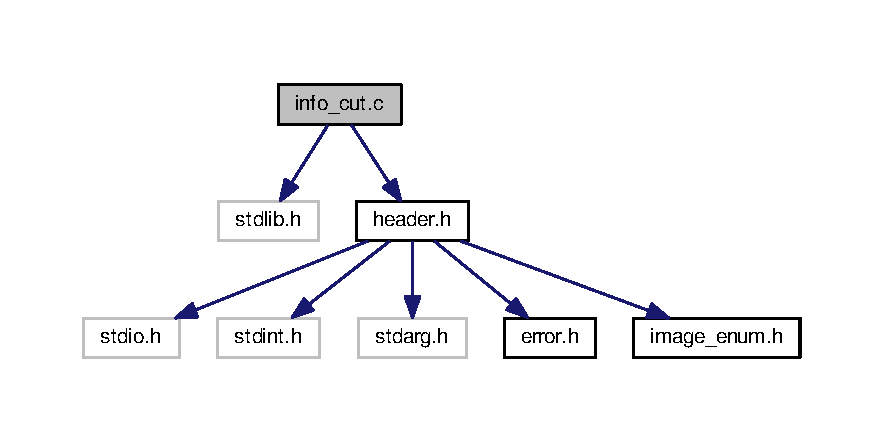
\includegraphics[width=350pt]{info__cut_8c__incl}
\end{center}
\end{figure}
\subsection*{Functions}
\begin{DoxyCompactItemize}
\item 
\hyperlink{header_8h_a3f4de920943cb4d0979d415b4c5e3989}{Imel\+Info\+Cut} $\ast$ \hyperlink{info__cut_8c_ad06ec44d23c494c1f501d03de880007e}{imel\+\_\+info\+\_\+cut\+\_\+new} (\hyperlink{header_8h_aef27fcac7a96d118b3c3194c2577049f}{Imel\+Orientation} orientation, \hyperlink{header_8h_af8a2b40c34eeed326846d0098ea84ec2}{Imel\+Size} position)
\begin{DoxyCompactList}\small\item\em Make a new guide. \end{DoxyCompactList}\item 
\hyperlink{header_8h_a3f4de920943cb4d0979d415b4c5e3989}{Imel\+Info\+Cut} $\ast$ \hyperlink{info__cut_8c_aa8e34152e2f5716e6a195ee1b8107f85}{imel\+\_\+info\+\_\+cut\+\_\+add} (\hyperlink{header_8h_a3f4de920943cb4d0979d415b4c5e3989}{Imel\+Info\+Cut} $\ast$cut\+\_\+info, \hyperlink{header_8h_aef27fcac7a96d118b3c3194c2577049f}{Imel\+Orientation} orientation, \hyperlink{header_8h_af8a2b40c34eeed326846d0098ea84ec2}{Imel\+Size} position)
\begin{DoxyCompactList}\small\item\em Add a guide line to existed list. \end{DoxyCompactList}\item 
\hyperlink{header_8h_a3f4de920943cb4d0979d415b4c5e3989}{Imel\+Info\+Cut} $\ast$ \hyperlink{info__cut_8c_a7d91db7c5670991c5480d2d642b2c05e}{imel\+\_\+info\+\_\+cut\+\_\+get\+\_\+index} (\hyperlink{header_8h_a3f4de920943cb4d0979d415b4c5e3989}{Imel\+Info\+Cut} $\ast$info\+\_\+cut, \hyperlink{header_8h_af8a2b40c34eeed326846d0098ea84ec2}{Imel\+Size} index)
\begin{DoxyCompactList}\small\item\em Get the element to a chosen index. \end{DoxyCompactList}\item 
\hyperlink{header_8h_a3f4de920943cb4d0979d415b4c5e3989}{Imel\+Info\+Cut} $\ast$ \hyperlink{info__cut_8c_a7de81c5bb96188056da6a3f623cc051a}{imel\+\_\+info\+\_\+cut\+\_\+copy\+\_\+index} (\hyperlink{header_8h_a3f4de920943cb4d0979d415b4c5e3989}{Imel\+Info\+Cut} $\ast$info\+\_\+cut, \hyperlink{header_8h_af8a2b40c34eeed326846d0098ea84ec2}{Imel\+Size} index)
\begin{DoxyCompactList}\small\item\em Copy the element to a chosen index. \end{DoxyCompactList}\item 
\hyperlink{header_8h_a3f4de920943cb4d0979d415b4c5e3989}{Imel\+Info\+Cut} $\ast$ \hyperlink{info__cut_8c_a7f6e806fc4c44dcec585faa0f98fd568}{imel\+\_\+info\+\_\+cut\+\_\+copy} (\hyperlink{header_8h_a3f4de920943cb4d0979d415b4c5e3989}{Imel\+Info\+Cut} $\ast$info\+\_\+cut)
\begin{DoxyCompactList}\small\item\em Duplicate a guide lines list. \end{DoxyCompactList}\item 
\hyperlink{header_8h_a3f4de920943cb4d0979d415b4c5e3989}{Imel\+Info\+Cut} $\ast$ \hyperlink{info__cut_8c_a8242b3f5a1f69a298d509dfab9940fa4}{imel\+\_\+info\+\_\+cut\+\_\+remove\+\_\+element} (\hyperlink{header_8h_a3f4de920943cb4d0979d415b4c5e3989}{Imel\+Info\+Cut} $\ast$cut\+\_\+info, \hyperlink{header_8h_af8a2b40c34eeed326846d0098ea84ec2}{Imel\+Size} index)
\begin{DoxyCompactList}\small\item\em Remove a guide line from a list. \end{DoxyCompactList}\item 
void \hyperlink{info__cut_8c_a73ba0a29544436cf4248c71a935560cd}{imel\+\_\+info\+\_\+cut\+\_\+free} (\hyperlink{header_8h_a3f4de920943cb4d0979d415b4c5e3989}{Imel\+Info\+Cut} $\ast$cut\+\_\+info)
\begin{DoxyCompactList}\small\item\em Free the memory of a guide lines list. \end{DoxyCompactList}\item 
void \hyperlink{info__cut_8c_a8ab936dfd037dbc4bf7fdeb3e746ae78}{imel\+\_\+info\+\_\+cut\+\_\+swap\+\_\+index} (\hyperlink{header_8h_a3f4de920943cb4d0979d415b4c5e3989}{Imel\+Info\+Cut} $\ast$cut\+\_\+info, \hyperlink{header_8h_af8a2b40c34eeed326846d0098ea84ec2}{Imel\+Size} index\+\_\+a, \hyperlink{header_8h_af8a2b40c34eeed326846d0098ea84ec2}{Imel\+Size} index\+\_\+b)
\begin{DoxyCompactList}\small\item\em Swap two element of a guide lines list. \end{DoxyCompactList}\item 
\hyperlink{header_8h_af8a2b40c34eeed326846d0098ea84ec2}{Imel\+Size} \hyperlink{info__cut_8c_a1a500fbdf3ddde14224fbf307f0162dc}{imel\+\_\+info\+\_\+cut\+\_\+count} (\hyperlink{header_8h_a3f4de920943cb4d0979d415b4c5e3989}{Imel\+Info\+Cut} $\ast$cut\+\_\+info)
\begin{DoxyCompactList}\small\item\em Count the element in a guide lines list. \end{DoxyCompactList}\item 
\hyperlink{header_8h_a3f4de920943cb4d0979d415b4c5e3989}{Imel\+Info\+Cut} $\ast$ \hyperlink{info__cut_8c_afcc7e864b9efccf6f68d5c17c4ac15f4}{imel\+\_\+info\+\_\+cut\+\_\+get\+\_\+next} (\hyperlink{header_8h_ad8298d38a89742ed84029b278c6acee5}{Imel\+Image} $\ast$image, \hyperlink{header_8h_a3f4de920943cb4d0979d415b4c5e3989}{Imel\+Info\+Cut} $\ast$cut\+\_\+info, \hyperlink{header_8h_af8a2b40c34eeed326846d0098ea84ec2}{Imel\+Size} index)
\begin{DoxyCompactList}\small\item\em Get the next guide line on the same axis. \end{DoxyCompactList}\item 
\hyperlink{header_8h_a3f4de920943cb4d0979d415b4c5e3989}{Imel\+Info\+Cut} $\ast$ \hyperlink{info__cut_8c_a0701899b2a5d8bfddfb3b8f1c630cc46}{imel\+\_\+info\+\_\+cut\+\_\+get\+\_\+prev} (\hyperlink{header_8h_ad8298d38a89742ed84029b278c6acee5}{Imel\+Image} $\ast$image, \hyperlink{header_8h_a3f4de920943cb4d0979d415b4c5e3989}{Imel\+Info\+Cut} $\ast$cut\+\_\+info, \hyperlink{header_8h_af8a2b40c34eeed326846d0098ea84ec2}{Imel\+Size} index)
\begin{DoxyCompactList}\small\item\em Get the previous guide line on the same axis. \end{DoxyCompactList}\item 
\hyperlink{header_8h_a3f4de920943cb4d0979d415b4c5e3989}{Imel\+Info\+Cut} $\ast$ \hyperlink{info__cut_8c_a9acfc735dbe2584b7baf13152e49e4a7}{imel\+\_\+info\+\_\+cut\+\_\+get\+\_\+min} (\hyperlink{header_8h_a3f4de920943cb4d0979d415b4c5e3989}{Imel\+Info\+Cut} $\ast$cut\+\_\+info, \hyperlink{header_8h_aef27fcac7a96d118b3c3194c2577049f}{Imel\+Orientation} orientation)
\begin{DoxyCompactList}\small\item\em Get the first guide line on the chosen axis. \end{DoxyCompactList}\item 
\hyperlink{header_8h_a3f4de920943cb4d0979d415b4c5e3989}{Imel\+Info\+Cut} $\ast$ \hyperlink{info__cut_8c_a9b8fef15e9ff4c43a111476fba37a338}{imel\+\_\+info\+\_\+cut\+\_\+get\+\_\+max} (\hyperlink{header_8h_a3f4de920943cb4d0979d415b4c5e3989}{Imel\+Info\+Cut} $\ast$cut\+\_\+info, \hyperlink{header_8h_aef27fcac7a96d118b3c3194c2577049f}{Imel\+Orientation} orientation)
\begin{DoxyCompactList}\small\item\em Get the last guide line on the chosen axis. \end{DoxyCompactList}\item 
\hyperlink{header_8h_af8a2b40c34eeed326846d0098ea84ec2}{Imel\+Size} \hyperlink{info__cut_8c_a796c4e05878ccbea05ed360906b05aab}{imel\+\_\+info\+\_\+cut\+\_\+get\+\_\+split} (\hyperlink{header_8h_ad8298d38a89742ed84029b278c6acee5}{Imel\+Image} $\ast$image, \hyperlink{header_8h_a3f4de920943cb4d0979d415b4c5e3989}{Imel\+Info\+Cut} $\ast$cut\+\_\+info, \hyperlink{header_8h_aef27fcac7a96d118b3c3194c2577049f}{Imel\+Orientation} orientation)
\begin{DoxyCompactList}\small\item\em Get the split number of an image. \end{DoxyCompactList}\end{DoxyCompactItemize}


\subsection{Detailed Description}
This file contains functions to operate with guide lines. 

\begin{DoxyAuthor}{Author}
Davide Francesco Merico 
\end{DoxyAuthor}


\subsection{Function Documentation}
\index{info\+\_\+cut.\+c@{info\+\_\+cut.\+c}!imel\+\_\+info\+\_\+cut\+\_\+add@{imel\+\_\+info\+\_\+cut\+\_\+add}}
\index{imel\+\_\+info\+\_\+cut\+\_\+add@{imel\+\_\+info\+\_\+cut\+\_\+add}!info\+\_\+cut.\+c@{info\+\_\+cut.\+c}}
\subsubsection[{\texorpdfstring{imel\+\_\+info\+\_\+cut\+\_\+add(\+Imel\+Info\+Cut $\ast$cut\+\_\+info, Imel\+Orientation orientation, Imel\+Size position)}{imel_info_cut_add(ImelInfoCut *cut_info, ImelOrientation orientation, ImelSize position)}}]{\setlength{\rightskip}{0pt plus 5cm}{\bf Imel\+Info\+Cut}$\ast$ imel\+\_\+info\+\_\+cut\+\_\+add (
\begin{DoxyParamCaption}
\item[{{\bf Imel\+Info\+Cut} $\ast$}]{cut\+\_\+info, }
\item[{{\bf Imel\+Orientation}}]{orientation, }
\item[{{\bf Imel\+Size}}]{position}
\end{DoxyParamCaption}
)}\hypertarget{info__cut_8c_aa8e34152e2f5716e6a195ee1b8107f85}{}\label{info__cut_8c_aa8e34152e2f5716e6a195ee1b8107f85}


Add a guide line to existed list. 

This function add a new guide line to an existed list.


\begin{DoxyParams}{Parameters}
{\em cut\+\_\+info} & Guide lines list \\
\hline
{\em orientation} & Guide line orientation \\
\hline
{\em position} & Guide line position on chosen axis \\
\hline
\end{DoxyParams}
\begin{DoxyReturn}{Returns}
Pointer to new start of {\ttfamily cut\+\_\+info} list or N\+U\+LL on error
\end{DoxyReturn}
\begin{DoxySeeAlso}{See also}
\hyperlink{header_8h_aef27fcac7a96d118b3c3194c2577049f}{Imel\+Orientation} 

\hyperlink{info__cut_8c_ad06ec44d23c494c1f501d03de880007e}{imel\+\_\+info\+\_\+cut\+\_\+new} 

\hyperlink{info__cut_8c_a8242b3f5a1f69a298d509dfab9940fa4}{imel\+\_\+info\+\_\+cut\+\_\+remove\+\_\+element} 
\end{DoxySeeAlso}
\index{info\+\_\+cut.\+c@{info\+\_\+cut.\+c}!imel\+\_\+info\+\_\+cut\+\_\+copy@{imel\+\_\+info\+\_\+cut\+\_\+copy}}
\index{imel\+\_\+info\+\_\+cut\+\_\+copy@{imel\+\_\+info\+\_\+cut\+\_\+copy}!info\+\_\+cut.\+c@{info\+\_\+cut.\+c}}
\subsubsection[{\texorpdfstring{imel\+\_\+info\+\_\+cut\+\_\+copy(\+Imel\+Info\+Cut $\ast$info\+\_\+cut)}{imel_info_cut_copy(ImelInfoCut *info_cut)}}]{\setlength{\rightskip}{0pt plus 5cm}{\bf Imel\+Info\+Cut}$\ast$ imel\+\_\+info\+\_\+cut\+\_\+copy (
\begin{DoxyParamCaption}
\item[{{\bf Imel\+Info\+Cut} $\ast$}]{info\+\_\+cut}
\end{DoxyParamCaption}
)}\hypertarget{info__cut_8c_a7f6e806fc4c44dcec585faa0f98fd568}{}\label{info__cut_8c_a7f6e806fc4c44dcec585faa0f98fd568}


Duplicate a guide lines list. 

This function duplicate the {\ttfamily info\+\_\+cut} list passed.


\begin{DoxyParams}{Parameters}
{\em info\+\_\+cut} & Guide lines list \\
\hline
\end{DoxyParams}
\begin{DoxyReturn}{Returns}
A copy of {\ttfamily info\+\_\+cut} 
\end{DoxyReturn}
\index{info\+\_\+cut.\+c@{info\+\_\+cut.\+c}!imel\+\_\+info\+\_\+cut\+\_\+copy\+\_\+index@{imel\+\_\+info\+\_\+cut\+\_\+copy\+\_\+index}}
\index{imel\+\_\+info\+\_\+cut\+\_\+copy\+\_\+index@{imel\+\_\+info\+\_\+cut\+\_\+copy\+\_\+index}!info\+\_\+cut.\+c@{info\+\_\+cut.\+c}}
\subsubsection[{\texorpdfstring{imel\+\_\+info\+\_\+cut\+\_\+copy\+\_\+index(\+Imel\+Info\+Cut $\ast$info\+\_\+cut, Imel\+Size index)}{imel_info_cut_copy_index(ImelInfoCut *info_cut, ImelSize index)}}]{\setlength{\rightskip}{0pt plus 5cm}{\bf Imel\+Info\+Cut}$\ast$ imel\+\_\+info\+\_\+cut\+\_\+copy\+\_\+index (
\begin{DoxyParamCaption}
\item[{{\bf Imel\+Info\+Cut} $\ast$}]{info\+\_\+cut, }
\item[{{\bf Imel\+Size}}]{index}
\end{DoxyParamCaption}
)}\hypertarget{info__cut_8c_a7de81c5bb96188056da6a3f623cc051a}{}\label{info__cut_8c_a7de81c5bb96188056da6a3f623cc051a}


Copy the element to a chosen index. 

This function copy the element in {\ttfamily info\+\_\+cut} which its index is equal to {\ttfamily index}.


\begin{DoxyParams}{Parameters}
{\em info\+\_\+cut} & Guide lines list \\
\hline
{\em index} & Chosen element index \\
\hline
\end{DoxyParams}
\begin{DoxyReturn}{Returns}
A new Imel\+Info\+Cut element or N\+U\+LL on error.
\end{DoxyReturn}
\begin{DoxySeeAlso}{See also}
\hyperlink{info__cut_8c_a7d91db7c5670991c5480d2d642b2c05e}{imel\+\_\+info\+\_\+cut\+\_\+get\+\_\+index} 

\hyperlink{info__cut_8c_a73ba0a29544436cf4248c71a935560cd}{imel\+\_\+info\+\_\+cut\+\_\+free} 
\end{DoxySeeAlso}
\index{info\+\_\+cut.\+c@{info\+\_\+cut.\+c}!imel\+\_\+info\+\_\+cut\+\_\+count@{imel\+\_\+info\+\_\+cut\+\_\+count}}
\index{imel\+\_\+info\+\_\+cut\+\_\+count@{imel\+\_\+info\+\_\+cut\+\_\+count}!info\+\_\+cut.\+c@{info\+\_\+cut.\+c}}
\subsubsection[{\texorpdfstring{imel\+\_\+info\+\_\+cut\+\_\+count(\+Imel\+Info\+Cut $\ast$cut\+\_\+info)}{imel_info_cut_count(ImelInfoCut *cut_info)}}]{\setlength{\rightskip}{0pt plus 5cm}{\bf Imel\+Size} imel\+\_\+info\+\_\+cut\+\_\+count (
\begin{DoxyParamCaption}
\item[{{\bf Imel\+Info\+Cut} $\ast$}]{cut\+\_\+info}
\end{DoxyParamCaption}
)}\hypertarget{info__cut_8c_a1a500fbdf3ddde14224fbf307f0162dc}{}\label{info__cut_8c_a1a500fbdf3ddde14224fbf307f0162dc}


Count the element in a guide lines list. 


\begin{DoxyParams}{Parameters}
{\em cut\+\_\+info} & Guide lines list \\
\hline
\end{DoxyParams}
\begin{DoxyReturn}{Returns}
Elements number or 0 on error.
\end{DoxyReturn}
\begin{DoxyNote}{Note}
Same as {\ttfamily cut\+\_\+info-\/$>$index + 1} 
\end{DoxyNote}
\index{info\+\_\+cut.\+c@{info\+\_\+cut.\+c}!imel\+\_\+info\+\_\+cut\+\_\+free@{imel\+\_\+info\+\_\+cut\+\_\+free}}
\index{imel\+\_\+info\+\_\+cut\+\_\+free@{imel\+\_\+info\+\_\+cut\+\_\+free}!info\+\_\+cut.\+c@{info\+\_\+cut.\+c}}
\subsubsection[{\texorpdfstring{imel\+\_\+info\+\_\+cut\+\_\+free(\+Imel\+Info\+Cut $\ast$cut\+\_\+info)}{imel_info_cut_free(ImelInfoCut *cut_info)}}]{\setlength{\rightskip}{0pt plus 5cm}void imel\+\_\+info\+\_\+cut\+\_\+free (
\begin{DoxyParamCaption}
\item[{{\bf Imel\+Info\+Cut} $\ast$}]{cut\+\_\+info}
\end{DoxyParamCaption}
)}\hypertarget{info__cut_8c_a73ba0a29544436cf4248c71a935560cd}{}\label{info__cut_8c_a73ba0a29544436cf4248c71a935560cd}


Free the memory of a guide lines list. 


\begin{DoxyParams}{Parameters}
{\em cut\+\_\+info} & Guide lines list to free\\
\hline
\end{DoxyParams}
\begin{DoxySeeAlso}{See also}
\hyperlink{info__cut_8c_ad06ec44d23c494c1f501d03de880007e}{imel\+\_\+info\+\_\+cut\+\_\+new} 
\end{DoxySeeAlso}
\index{info\+\_\+cut.\+c@{info\+\_\+cut.\+c}!imel\+\_\+info\+\_\+cut\+\_\+get\+\_\+index@{imel\+\_\+info\+\_\+cut\+\_\+get\+\_\+index}}
\index{imel\+\_\+info\+\_\+cut\+\_\+get\+\_\+index@{imel\+\_\+info\+\_\+cut\+\_\+get\+\_\+index}!info\+\_\+cut.\+c@{info\+\_\+cut.\+c}}
\subsubsection[{\texorpdfstring{imel\+\_\+info\+\_\+cut\+\_\+get\+\_\+index(\+Imel\+Info\+Cut $\ast$info\+\_\+cut, Imel\+Size index)}{imel_info_cut_get_index(ImelInfoCut *info_cut, ImelSize index)}}]{\setlength{\rightskip}{0pt plus 5cm}{\bf Imel\+Info\+Cut}$\ast$ imel\+\_\+info\+\_\+cut\+\_\+get\+\_\+index (
\begin{DoxyParamCaption}
\item[{{\bf Imel\+Info\+Cut} $\ast$}]{info\+\_\+cut, }
\item[{{\bf Imel\+Size}}]{index}
\end{DoxyParamCaption}
)}\hypertarget{info__cut_8c_a7d91db7c5670991c5480d2d642b2c05e}{}\label{info__cut_8c_a7d91db7c5670991c5480d2d642b2c05e}


Get the element to a chosen index. 

This function get the element in {\ttfamily info\+\_\+cut} which its index is equal to {\ttfamily index}.


\begin{DoxyParams}{Parameters}
{\em info\+\_\+cut} & Guide lines list \\
\hline
{\em index} & Chosen element index \\
\hline
\end{DoxyParams}
\begin{DoxyReturn}{Returns}
A pointer to the element if found it or N\+U\+LL on error 
\end{DoxyReturn}
\index{info\+\_\+cut.\+c@{info\+\_\+cut.\+c}!imel\+\_\+info\+\_\+cut\+\_\+get\+\_\+max@{imel\+\_\+info\+\_\+cut\+\_\+get\+\_\+max}}
\index{imel\+\_\+info\+\_\+cut\+\_\+get\+\_\+max@{imel\+\_\+info\+\_\+cut\+\_\+get\+\_\+max}!info\+\_\+cut.\+c@{info\+\_\+cut.\+c}}
\subsubsection[{\texorpdfstring{imel\+\_\+info\+\_\+cut\+\_\+get\+\_\+max(\+Imel\+Info\+Cut $\ast$cut\+\_\+info, Imel\+Orientation orientation)}{imel_info_cut_get_max(ImelInfoCut *cut_info, ImelOrientation orientation)}}]{\setlength{\rightskip}{0pt plus 5cm}{\bf Imel\+Info\+Cut}$\ast$ imel\+\_\+info\+\_\+cut\+\_\+get\+\_\+max (
\begin{DoxyParamCaption}
\item[{{\bf Imel\+Info\+Cut} $\ast$}]{cut\+\_\+info, }
\item[{{\bf Imel\+Orientation}}]{orientation}
\end{DoxyParamCaption}
)}\hypertarget{info__cut_8c_a9b8fef15e9ff4c43a111476fba37a338}{}\label{info__cut_8c_a9b8fef15e9ff4c43a111476fba37a338}


Get the last guide line on the chosen axis. 


\begin{DoxyParams}{Parameters}
{\em cut\+\_\+info} & Guide lines list \\
\hline
{\em orientation} & Reference axis \\
\hline
\end{DoxyParams}
\begin{DoxyReturn}{Returns}
A pointer to the last guide line, based on it position or N\+U\+LL on error.
\end{DoxyReturn}
\begin{DoxySeeAlso}{See also}
\hyperlink{info__cut_8c_a9acfc735dbe2584b7baf13152e49e4a7}{imel\+\_\+info\+\_\+cut\+\_\+get\+\_\+min} 

\hyperlink{info__cut_8c_a0701899b2a5d8bfddfb3b8f1c630cc46}{imel\+\_\+info\+\_\+cut\+\_\+get\+\_\+prev} 
\end{DoxySeeAlso}
\index{info\+\_\+cut.\+c@{info\+\_\+cut.\+c}!imel\+\_\+info\+\_\+cut\+\_\+get\+\_\+min@{imel\+\_\+info\+\_\+cut\+\_\+get\+\_\+min}}
\index{imel\+\_\+info\+\_\+cut\+\_\+get\+\_\+min@{imel\+\_\+info\+\_\+cut\+\_\+get\+\_\+min}!info\+\_\+cut.\+c@{info\+\_\+cut.\+c}}
\subsubsection[{\texorpdfstring{imel\+\_\+info\+\_\+cut\+\_\+get\+\_\+min(\+Imel\+Info\+Cut $\ast$cut\+\_\+info, Imel\+Orientation orientation)}{imel_info_cut_get_min(ImelInfoCut *cut_info, ImelOrientation orientation)}}]{\setlength{\rightskip}{0pt plus 5cm}{\bf Imel\+Info\+Cut}$\ast$ imel\+\_\+info\+\_\+cut\+\_\+get\+\_\+min (
\begin{DoxyParamCaption}
\item[{{\bf Imel\+Info\+Cut} $\ast$}]{cut\+\_\+info, }
\item[{{\bf Imel\+Orientation}}]{orientation}
\end{DoxyParamCaption}
)}\hypertarget{info__cut_8c_a9acfc735dbe2584b7baf13152e49e4a7}{}\label{info__cut_8c_a9acfc735dbe2584b7baf13152e49e4a7}


Get the first guide line on the chosen axis. 


\begin{DoxyParams}{Parameters}
{\em cut\+\_\+info} & Guide lines list \\
\hline
{\em orientation} & Reference axis \\
\hline
\end{DoxyParams}
\begin{DoxyReturn}{Returns}
A pointer to the first guide line, based on it position or N\+U\+LL on error.
\end{DoxyReturn}
\begin{DoxySeeAlso}{See also}
\hyperlink{info__cut_8c_a9b8fef15e9ff4c43a111476fba37a338}{imel\+\_\+info\+\_\+cut\+\_\+get\+\_\+max} 

\hyperlink{info__cut_8c_afcc7e864b9efccf6f68d5c17c4ac15f4}{imel\+\_\+info\+\_\+cut\+\_\+get\+\_\+next} 
\end{DoxySeeAlso}
\index{info\+\_\+cut.\+c@{info\+\_\+cut.\+c}!imel\+\_\+info\+\_\+cut\+\_\+get\+\_\+next@{imel\+\_\+info\+\_\+cut\+\_\+get\+\_\+next}}
\index{imel\+\_\+info\+\_\+cut\+\_\+get\+\_\+next@{imel\+\_\+info\+\_\+cut\+\_\+get\+\_\+next}!info\+\_\+cut.\+c@{info\+\_\+cut.\+c}}
\subsubsection[{\texorpdfstring{imel\+\_\+info\+\_\+cut\+\_\+get\+\_\+next(\+Imel\+Image $\ast$image, Imel\+Info\+Cut $\ast$cut\+\_\+info, Imel\+Size index)}{imel_info_cut_get_next(ImelImage *image, ImelInfoCut *cut_info, ImelSize index)}}]{\setlength{\rightskip}{0pt plus 5cm}{\bf Imel\+Info\+Cut}$\ast$ imel\+\_\+info\+\_\+cut\+\_\+get\+\_\+next (
\begin{DoxyParamCaption}
\item[{{\bf Imel\+Image} $\ast$}]{image, }
\item[{{\bf Imel\+Info\+Cut} $\ast$}]{cut\+\_\+info, }
\item[{{\bf Imel\+Size}}]{index}
\end{DoxyParamCaption}
)}\hypertarget{info__cut_8c_afcc7e864b9efccf6f68d5c17c4ac15f4}{}\label{info__cut_8c_afcc7e864b9efccf6f68d5c17c4ac15f4}


Get the next guide line on the same axis. 


\begin{DoxyParams}{Parameters}
{\em image} & Image reference for the guide lines \\
\hline
{\em cut\+\_\+info} & Guide lines list \\
\hline
{\em index} & Index of the current guide line \\
\hline
\end{DoxyParams}
\begin{DoxyReturn}{Returns}
A pointer to the next guide line, based on their position, or N\+U\+LL on error.
\end{DoxyReturn}
\begin{DoxySeeAlso}{See also}
\hyperlink{info__cut_8c_a0701899b2a5d8bfddfb3b8f1c630cc46}{imel\+\_\+info\+\_\+cut\+\_\+get\+\_\+prev} 
\end{DoxySeeAlso}
\index{info\+\_\+cut.\+c@{info\+\_\+cut.\+c}!imel\+\_\+info\+\_\+cut\+\_\+get\+\_\+prev@{imel\+\_\+info\+\_\+cut\+\_\+get\+\_\+prev}}
\index{imel\+\_\+info\+\_\+cut\+\_\+get\+\_\+prev@{imel\+\_\+info\+\_\+cut\+\_\+get\+\_\+prev}!info\+\_\+cut.\+c@{info\+\_\+cut.\+c}}
\subsubsection[{\texorpdfstring{imel\+\_\+info\+\_\+cut\+\_\+get\+\_\+prev(\+Imel\+Image $\ast$image, Imel\+Info\+Cut $\ast$cut\+\_\+info, Imel\+Size index)}{imel_info_cut_get_prev(ImelImage *image, ImelInfoCut *cut_info, ImelSize index)}}]{\setlength{\rightskip}{0pt plus 5cm}{\bf Imel\+Info\+Cut}$\ast$ imel\+\_\+info\+\_\+cut\+\_\+get\+\_\+prev (
\begin{DoxyParamCaption}
\item[{{\bf Imel\+Image} $\ast$}]{image, }
\item[{{\bf Imel\+Info\+Cut} $\ast$}]{cut\+\_\+info, }
\item[{{\bf Imel\+Size}}]{index}
\end{DoxyParamCaption}
)}\hypertarget{info__cut_8c_a0701899b2a5d8bfddfb3b8f1c630cc46}{}\label{info__cut_8c_a0701899b2a5d8bfddfb3b8f1c630cc46}


Get the previous guide line on the same axis. 


\begin{DoxyParams}{Parameters}
{\em image} & Image reference for the guide lines \\
\hline
{\em cut\+\_\+info} & Guide lines list \\
\hline
{\em index} & Index of the current guide line \\
\hline
\end{DoxyParams}
\begin{DoxyReturn}{Returns}
A pointer to the previous guide line, based on their position, or N\+U\+LL on error.
\end{DoxyReturn}
\begin{DoxySeeAlso}{See also}
\hyperlink{info__cut_8c_afcc7e864b9efccf6f68d5c17c4ac15f4}{imel\+\_\+info\+\_\+cut\+\_\+get\+\_\+next} 
\end{DoxySeeAlso}
\index{info\+\_\+cut.\+c@{info\+\_\+cut.\+c}!imel\+\_\+info\+\_\+cut\+\_\+get\+\_\+split@{imel\+\_\+info\+\_\+cut\+\_\+get\+\_\+split}}
\index{imel\+\_\+info\+\_\+cut\+\_\+get\+\_\+split@{imel\+\_\+info\+\_\+cut\+\_\+get\+\_\+split}!info\+\_\+cut.\+c@{info\+\_\+cut.\+c}}
\subsubsection[{\texorpdfstring{imel\+\_\+info\+\_\+cut\+\_\+get\+\_\+split(\+Imel\+Image $\ast$image, Imel\+Info\+Cut $\ast$cut\+\_\+info, Imel\+Orientation orientation)}{imel_info_cut_get_split(ImelImage *image, ImelInfoCut *cut_info, ImelOrientation orientation)}}]{\setlength{\rightskip}{0pt plus 5cm}{\bf Imel\+Size} imel\+\_\+info\+\_\+cut\+\_\+get\+\_\+split (
\begin{DoxyParamCaption}
\item[{{\bf Imel\+Image} $\ast$}]{image, }
\item[{{\bf Imel\+Info\+Cut} $\ast$}]{cut\+\_\+info, }
\item[{{\bf Imel\+Orientation}}]{orientation}
\end{DoxyParamCaption}
)}\hypertarget{info__cut_8c_a796c4e05878ccbea05ed360906b05aab}{}\label{info__cut_8c_a796c4e05878ccbea05ed360906b05aab}


Get the split number of an image. 

This function get the number of the areas which the {\ttfamily image} will be splitted if cutted with the guide lines in {\ttfamily cut\+\_\+info} list.


\begin{DoxyParams}{Parameters}
{\em image} & Image reference \\
\hline
{\em cut\+\_\+info} & Guide lines list \\
\hline
{\em orientation} & Reference axis \\
\hline
\end{DoxyParams}
\begin{DoxyReturn}{Returns}
The number of areas resulted by hypotetical cuts 
\end{DoxyReturn}
\index{info\+\_\+cut.\+c@{info\+\_\+cut.\+c}!imel\+\_\+info\+\_\+cut\+\_\+new@{imel\+\_\+info\+\_\+cut\+\_\+new}}
\index{imel\+\_\+info\+\_\+cut\+\_\+new@{imel\+\_\+info\+\_\+cut\+\_\+new}!info\+\_\+cut.\+c@{info\+\_\+cut.\+c}}
\subsubsection[{\texorpdfstring{imel\+\_\+info\+\_\+cut\+\_\+new(\+Imel\+Orientation orientation, Imel\+Size position)}{imel_info_cut_new(ImelOrientation orientation, ImelSize position)}}]{\setlength{\rightskip}{0pt plus 5cm}{\bf Imel\+Info\+Cut}$\ast$ imel\+\_\+info\+\_\+cut\+\_\+new (
\begin{DoxyParamCaption}
\item[{{\bf Imel\+Orientation}}]{orientation, }
\item[{{\bf Imel\+Size}}]{position}
\end{DoxyParamCaption}
)}\hypertarget{info__cut_8c_ad06ec44d23c494c1f501d03de880007e}{}\label{info__cut_8c_ad06ec44d23c494c1f501d03de880007e}


Make a new guide. 

This function make a new guide line with a chosen {\ttfamily orientation} and {\ttfamily position}.


\begin{DoxyParams}{Parameters}
{\em orientation} & Guide line orientation \\
\hline
{\em position} & Guide line position on chosen axis \\
\hline
\end{DoxyParams}
\begin{DoxyReturn}{Returns}
A new guide line or N\+U\+LL on error.
\end{DoxyReturn}
\begin{DoxySeeAlso}{See also}
\hyperlink{header_8h_aef27fcac7a96d118b3c3194c2577049f}{Imel\+Orientation} 

\hyperlink{info__cut_8c_aa8e34152e2f5716e6a195ee1b8107f85}{imel\+\_\+info\+\_\+cut\+\_\+add} 

\hyperlink{info__cut_8c_a73ba0a29544436cf4248c71a935560cd}{imel\+\_\+info\+\_\+cut\+\_\+free} 
\end{DoxySeeAlso}
\index{info\+\_\+cut.\+c@{info\+\_\+cut.\+c}!imel\+\_\+info\+\_\+cut\+\_\+remove\+\_\+element@{imel\+\_\+info\+\_\+cut\+\_\+remove\+\_\+element}}
\index{imel\+\_\+info\+\_\+cut\+\_\+remove\+\_\+element@{imel\+\_\+info\+\_\+cut\+\_\+remove\+\_\+element}!info\+\_\+cut.\+c@{info\+\_\+cut.\+c}}
\subsubsection[{\texorpdfstring{imel\+\_\+info\+\_\+cut\+\_\+remove\+\_\+element(\+Imel\+Info\+Cut $\ast$cut\+\_\+info, Imel\+Size index)}{imel_info_cut_remove_element(ImelInfoCut *cut_info, ImelSize index)}}]{\setlength{\rightskip}{0pt plus 5cm}{\bf Imel\+Info\+Cut}$\ast$ imel\+\_\+info\+\_\+cut\+\_\+remove\+\_\+element (
\begin{DoxyParamCaption}
\item[{{\bf Imel\+Info\+Cut} $\ast$}]{cut\+\_\+info, }
\item[{{\bf Imel\+Size}}]{index}
\end{DoxyParamCaption}
)}\hypertarget{info__cut_8c_a8242b3f5a1f69a298d509dfab9940fa4}{}\label{info__cut_8c_a8242b3f5a1f69a298d509dfab9940fa4}


Remove a guide line from a list. 

This function remove the element which index is equal to {\ttfamily index} in the {\ttfamily cut\+\_\+info} list.


\begin{DoxyParams}{Parameters}
{\em cut\+\_\+info} & Guide lines list \\
\hline
{\em index} & Index of the element to remove \\
\hline
\end{DoxyParams}
\begin{DoxyReturn}{Returns}
A pointer to the start of the {\ttfamily cut\+\_\+info} passed
\end{DoxyReturn}
\begin{DoxySeeAlso}{See also}
\hyperlink{info__cut_8c_aa8e34152e2f5716e6a195ee1b8107f85}{imel\+\_\+info\+\_\+cut\+\_\+add} 
\end{DoxySeeAlso}
\index{info\+\_\+cut.\+c@{info\+\_\+cut.\+c}!imel\+\_\+info\+\_\+cut\+\_\+swap\+\_\+index@{imel\+\_\+info\+\_\+cut\+\_\+swap\+\_\+index}}
\index{imel\+\_\+info\+\_\+cut\+\_\+swap\+\_\+index@{imel\+\_\+info\+\_\+cut\+\_\+swap\+\_\+index}!info\+\_\+cut.\+c@{info\+\_\+cut.\+c}}
\subsubsection[{\texorpdfstring{imel\+\_\+info\+\_\+cut\+\_\+swap\+\_\+index(\+Imel\+Info\+Cut $\ast$cut\+\_\+info, Imel\+Size index\+\_\+a, Imel\+Size index\+\_\+b)}{imel_info_cut_swap_index(ImelInfoCut *cut_info, ImelSize index_a, ImelSize index_b)}}]{\setlength{\rightskip}{0pt plus 5cm}void imel\+\_\+info\+\_\+cut\+\_\+swap\+\_\+index (
\begin{DoxyParamCaption}
\item[{{\bf Imel\+Info\+Cut} $\ast$}]{cut\+\_\+info, }
\item[{{\bf Imel\+Size}}]{index\+\_\+a, }
\item[{{\bf Imel\+Size}}]{index\+\_\+b}
\end{DoxyParamCaption}
)}\hypertarget{info__cut_8c_a8ab936dfd037dbc4bf7fdeb3e746ae78}{}\label{info__cut_8c_a8ab936dfd037dbc4bf7fdeb3e746ae78}


Swap two element of a guide lines list. 

This function swap the element at index {\ttfamily index\+\_\+a} with the element at index {\ttfamily index\+\_\+b}.


\begin{DoxyParams}{Parameters}
{\em cut\+\_\+info} & Guide lines list \\
\hline
{\em index\+\_\+a} & Index of the first element \\
\hline
{\em index\+\_\+b} & Index of the second element \\
\hline
\end{DoxyParams}

\hypertarget{miscellaneous_8c}{}\section{miscellaneous.\+c File Reference}
\label{miscellaneous_8c}\index{miscellaneous.\+c@{miscellaneous.\+c}}


This file contains miscellaneus function.  


{\ttfamily \#include \char`\"{}header.\+h\char`\"{}}\\*
Include dependency graph for miscellaneous.\+c\+:
\nopagebreak
\begin{figure}[H]
\begin{center}
\leavevmode
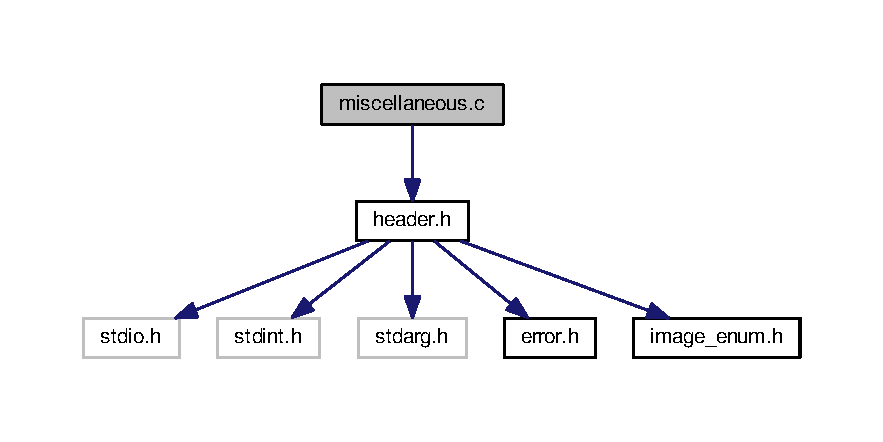
\includegraphics[width=350pt]{miscellaneous_8c__incl}
\end{center}
\end{figure}
\subsection*{Functions}
\begin{DoxyCompactItemize}
\item 
\hyperlink{header_8h_a669b28ed18156f1a4f13732e070d6cf2}{bool} \hyperlink{miscellaneous_8c_acf020a7e381aafaa9ee87f8b91994c73}{imel\+\_\+enable\+\_\+brush} (\hyperlink{header_8h_ad8298d38a89742ed84029b278c6acee5}{Imel\+Image} $\ast$brush)
\begin{DoxyCompactList}\small\item\em Enable the brush. \end{DoxyCompactList}\item 
\hyperlink{header_8h_a669b28ed18156f1a4f13732e070d6cf2}{bool} \hyperlink{miscellaneous_8c_abd21a9ca5c598a94d94e99102968916d}{imel\+\_\+disable\+\_\+brush} (void)
\begin{DoxyCompactList}\small\item\em Disable the brush. \end{DoxyCompactList}\item 
\hyperlink{header_8h_a669b28ed18156f1a4f13732e070d6cf2}{bool} \hyperlink{miscellaneous_8c_ad4629c597b8f8827434c9ca3b183c4de}{imel\+\_\+printf\+\_\+debug} (const char $\ast$function, const char $\ast$filename, const char $\ast$error\+\_\+level, char $\ast$\+\_\+\+\_\+format,...)
\end{DoxyCompactItemize}
\subsection*{Variables}
\begin{DoxyCompactItemize}
\item 
\hyperlink{header_8h_ad8298d38a89742ed84029b278c6acee5}{Imel\+Image} $\ast$ \hyperlink{miscellaneous_8c_a321f8f9d07d202b736865ab1c4717169}{global\+\_\+brush}
\end{DoxyCompactItemize}


\subsection{Detailed Description}
This file contains miscellaneus function. 

\begin{DoxyAuthor}{Author}
Davide Francesco Merico 
\end{DoxyAuthor}


\subsection{Function Documentation}
\index{miscellaneous.\+c@{miscellaneous.\+c}!imel\+\_\+disable\+\_\+brush@{imel\+\_\+disable\+\_\+brush}}
\index{imel\+\_\+disable\+\_\+brush@{imel\+\_\+disable\+\_\+brush}!miscellaneous.\+c@{miscellaneous.\+c}}
\subsubsection[{\texorpdfstring{imel\+\_\+disable\+\_\+brush(void)}{imel_disable_brush(void)}}]{\setlength{\rightskip}{0pt plus 5cm}{\bf bool} imel\+\_\+disable\+\_\+brush (
\begin{DoxyParamCaption}
\item[{void}]{}
\end{DoxyParamCaption}
)}\hypertarget{miscellaneous_8c_abd21a9ca5c598a94d94e99102968916d}{}\label{miscellaneous_8c_abd21a9ca5c598a94d94e99102968916d}


Disable the brush. 

\begin{DoxyReturn}{Returns}
T\+R\+UE on success, F\+A\+L\+SE on error.
\end{DoxyReturn}
\begin{DoxySeeAlso}{See also}
\hyperlink{miscellaneous_8c_a321f8f9d07d202b736865ab1c4717169}{global\+\_\+brush} 

\hyperlink{miscellaneous_8c_abd21a9ca5c598a94d94e99102968916d}{imel\+\_\+disable\+\_\+brush} 
\end{DoxySeeAlso}
\index{miscellaneous.\+c@{miscellaneous.\+c}!imel\+\_\+enable\+\_\+brush@{imel\+\_\+enable\+\_\+brush}}
\index{imel\+\_\+enable\+\_\+brush@{imel\+\_\+enable\+\_\+brush}!miscellaneous.\+c@{miscellaneous.\+c}}
\subsubsection[{\texorpdfstring{imel\+\_\+enable\+\_\+brush(\+Imel\+Image $\ast$brush)}{imel_enable_brush(ImelImage *brush)}}]{\setlength{\rightskip}{0pt plus 5cm}{\bf bool} imel\+\_\+enable\+\_\+brush (
\begin{DoxyParamCaption}
\item[{{\bf Imel\+Image} $\ast$}]{brush}
\end{DoxyParamCaption}
)}\hypertarget{miscellaneous_8c_acf020a7e381aafaa9ee87f8b91994c73}{}\label{miscellaneous_8c_acf020a7e381aafaa9ee87f8b91994c73}


Enable the brush. 


\begin{DoxyParams}{Parameters}
{\em brush} & Image containing the brush \\
\hline
\end{DoxyParams}
\begin{DoxyReturn}{Returns}
T\+R\+UE on success, F\+A\+L\+SE on error.
\end{DoxyReturn}
\begin{DoxySeeAlso}{See also}
\hyperlink{miscellaneous_8c_a321f8f9d07d202b736865ab1c4717169}{global\+\_\+brush} 

\hyperlink{miscellaneous_8c_abd21a9ca5c598a94d94e99102968916d}{imel\+\_\+disable\+\_\+brush} 
\end{DoxySeeAlso}
\index{miscellaneous.\+c@{miscellaneous.\+c}!imel\+\_\+printf\+\_\+debug@{imel\+\_\+printf\+\_\+debug}}
\index{imel\+\_\+printf\+\_\+debug@{imel\+\_\+printf\+\_\+debug}!miscellaneous.\+c@{miscellaneous.\+c}}
\subsubsection[{\texorpdfstring{imel\+\_\+printf\+\_\+debug(const char $\ast$function, const char $\ast$filename, const char $\ast$error\+\_\+level, char $\ast$\+\_\+\+\_\+format,...)}{imel_printf_debug(const char *function, const char *filename, const char *error_level, char *__format,...)}}]{\setlength{\rightskip}{0pt plus 5cm}{\bf bool} imel\+\_\+printf\+\_\+debug (
\begin{DoxyParamCaption}
\item[{const char $\ast$}]{function, }
\item[{const char $\ast$}]{filename, }
\item[{const char $\ast$}]{error\+\_\+level, }
\item[{char $\ast$}]{\+\_\+\+\_\+format, }
\item[{}]{...}
\end{DoxyParamCaption}
)}\hypertarget{miscellaneous_8c_ad4629c597b8f8827434c9ca3b183c4de}{}\label{miscellaneous_8c_ad4629c597b8f8827434c9ca3b183c4de}
imel\+\_\+debug\+\_\+printf are foundamental for macro \hyperlink{header_8h_afa6c4a6400518363dd86d406785585b2}{return\+\_\+if\+\_\+fail} and \hyperlink{header_8h_aedf541d4162f35857638d2ececedc2d7}{return\+\_\+var\+\_\+if\+\_\+fail}. It print the message only if compiled with debug=true.


\begin{DoxyParams}{Parameters}
{\em function} & Name of the function where it\textquotesingle{}s called or N\+U\+LL \\
\hline
{\em filename} & Name of the file or N\+U\+LL \\
\hline
{\em error\+\_\+level} & Type of error ( Warning, Error, Info, ... ) or N\+U\+LL \\
\hline
{\em \+\_\+\+\_\+format} & Message \\
\hline
{\em ...} & Parameters requested by {\ttfamily \+\_\+\+\_\+format} \\
\hline
\end{DoxyParams}
\begin{DoxyReturn}{Returns}
T\+R\+UE if debug=true, else F\+A\+L\+SE 
\end{DoxyReturn}


\subsection{Variable Documentation}
\index{miscellaneous.\+c@{miscellaneous.\+c}!global\+\_\+brush@{global\+\_\+brush}}
\index{global\+\_\+brush@{global\+\_\+brush}!miscellaneous.\+c@{miscellaneous.\+c}}
\subsubsection[{\texorpdfstring{global\+\_\+brush}{global_brush}}]{\setlength{\rightskip}{0pt plus 5cm}{\bf Imel\+Image}$\ast$ global\+\_\+brush}\hypertarget{miscellaneous_8c_a321f8f9d07d202b736865ab1c4717169}{}\label{miscellaneous_8c_a321f8f9d07d202b736865ab1c4717169}
If brush is enabled, this variable will contain the brush image and will be used in all drawing functions except \hyperlink{draw_8c_a80e6d667aceb3de202823e5493a774b1}{imel\+\_\+draw\+\_\+point}. 
\hypertarget{pixel_8c}{}\section{pixel.\+c File Reference}
\label{pixel_8c}\index{pixel.\+c@{pixel.\+c}}


This file contains functions to operate with guide lines.  


{\ttfamily \#include $<$stdlib.\+h$>$}\\*
{\ttfamily \#include $<$string.\+h$>$}\\*
{\ttfamily \#include $<$ctype.\+h$>$}\\*
{\ttfamily \#include $<$math.\+h$>$}\\*
{\ttfamily \#include \char`\"{}header.\+h\char`\"{}}\\*
Include dependency graph for pixel.\+c\+:
\nopagebreak
\begin{figure}[H]
\begin{center}
\leavevmode
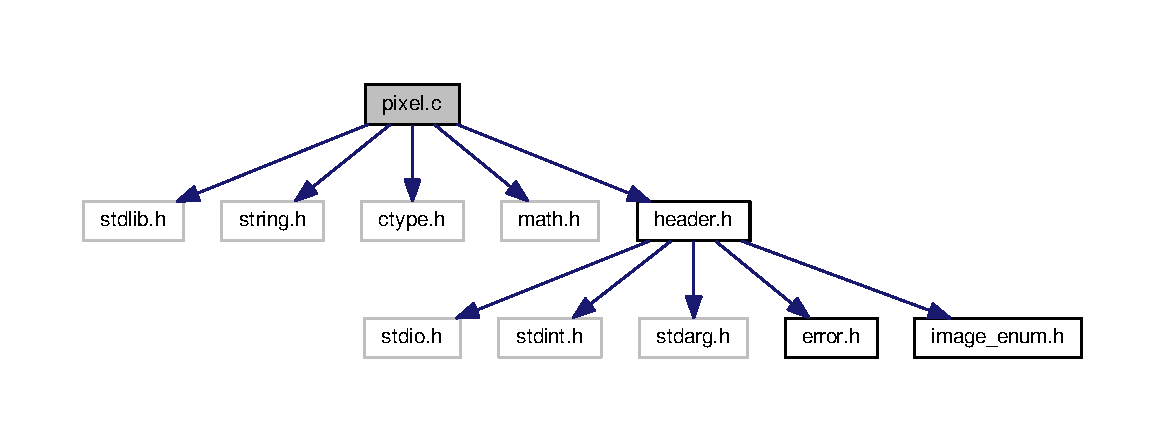
\includegraphics[width=350pt]{pixel_8c__incl}
\end{center}
\end{figure}
\subsection*{Functions}
\begin{DoxyCompactItemize}
\item 
\hyperlink{header_8h_add7dd9f8c093208bc4fd135a22a670ba}{Imel\+Pixel} \hyperlink{pixel_8c_acafccb8e6ccf0cb329498d8343ba1775}{imel\+\_\+pixel\+\_\+union} (\hyperlink{header_8h_add7dd9f8c093208bc4fd135a22a670ba}{Imel\+Pixel} a, \hyperlink{header_8h_add7dd9f8c093208bc4fd135a22a670ba}{Imel\+Pixel} b, unsigned char \+\_\+opacity)
\begin{DoxyCompactList}\small\item\em Join two pixel with a chosen opacity. \end{DoxyCompactList}\item 
\hyperlink{header_8h_add7dd9f8c093208bc4fd135a22a670ba}{Imel\+Pixel} \hyperlink{pixel_8c_aaf2dba6a30b6612b7c1730195935a88d}{imel\+\_\+pixel\+\_\+new} (\hyperlink{header_8h_add1326f75f0c1a7da9f14c2ed4f673e9}{Imel\+Color} red, \hyperlink{header_8h_add1326f75f0c1a7da9f14c2ed4f673e9}{Imel\+Color} green, \hyperlink{header_8h_add1326f75f0c1a7da9f14c2ed4f673e9}{Imel\+Color} blue, \hyperlink{header_8h_a97bc4b146a807c2d83b966983132f4fc}{Imel\+Level} level)
\begin{DoxyCompactList}\small\item\em Make a new pixel. \end{DoxyCompactList}\item 
\hyperlink{header_8h_add7dd9f8c093208bc4fd135a22a670ba}{Imel\+Pixel} \hyperlink{pixel_8c_a0d1c4cb614847e8084854f40d05d0eb7}{imel\+\_\+pixel\+\_\+new\+\_\+from\+\_\+string} (const char $\ast$string, \hyperlink{header_8h_a97bc4b146a807c2d83b966983132f4fc}{Imel\+Level} level)
\begin{DoxyCompactList}\small\item\em Make a new pixel from a string. \end{DoxyCompactList}\item 
void \hyperlink{pixel_8c_a46e21819169c162fbea522318638770a}{imel\+\_\+pixel\+\_\+set} (\hyperlink{header_8h_add7dd9f8c093208bc4fd135a22a670ba}{Imel\+Pixel} $\ast$pixel, \hyperlink{header_8h_add1326f75f0c1a7da9f14c2ed4f673e9}{Imel\+Color} red, \hyperlink{header_8h_add1326f75f0c1a7da9f14c2ed4f673e9}{Imel\+Color} green, \hyperlink{header_8h_add1326f75f0c1a7da9f14c2ed4f673e9}{Imel\+Color} blue, \hyperlink{header_8h_a97bc4b146a807c2d83b966983132f4fc}{Imel\+Level} level)
\begin{DoxyCompactList}\small\item\em Set a new value for a pixel. \end{DoxyCompactList}\item 
double \hyperlink{pixel_8c_a99414f31f8c6163710380d1c680e6360}{imel\+\_\+pixel\+\_\+get\+\_\+distance} (\hyperlink{header_8h_add7dd9f8c093208bc4fd135a22a670ba}{Imel\+Pixel} a, \hyperlink{header_8h_add7dd9f8c093208bc4fd135a22a670ba}{Imel\+Pixel} b)
\begin{DoxyCompactList}\small\item\em Get the chromatic distance between two colors. \end{DoxyCompactList}\item 
void \hyperlink{pixel_8c_ae756974e96560e68b72efa41aafd3d4a}{imel\+\_\+pixel\+\_\+set\+\_\+from\+\_\+pixel} (\hyperlink{header_8h_add7dd9f8c093208bc4fd135a22a670ba}{Imel\+Pixel} $\ast$pixel, \hyperlink{header_8h_add7dd9f8c093208bc4fd135a22a670ba}{Imel\+Pixel} pxl)
\begin{DoxyCompactList}\small\item\em Copy the values of a pixel in another one. \end{DoxyCompactList}\item 
void \hyperlink{pixel_8c_af690161266179d255e4f8394b74ef08f}{imel\+\_\+pixel\+\_\+set\+\_\+from\+\_\+string} (\hyperlink{header_8h_add7dd9f8c093208bc4fd135a22a670ba}{Imel\+Pixel} $\ast$pixel, const char $\ast$string, \hyperlink{header_8h_a97bc4b146a807c2d83b966983132f4fc}{Imel\+Level} level)
\begin{DoxyCompactList}\small\item\em Set a new value for a pixel from a string. \end{DoxyCompactList}\item 
void \hyperlink{pixel_8c_a9bc6aa8b3ec663f1635827b0ebbdf46a}{imel\+\_\+pixel\+\_\+copy} (\hyperlink{header_8h_add7dd9f8c093208bc4fd135a22a670ba}{Imel\+Pixel} $\ast$dest, \hyperlink{header_8h_add7dd9f8c093208bc4fd135a22a670ba}{Imel\+Pixel} src)
\begin{DoxyCompactList}\small\item\em Copy a pixel over another one. \end{DoxyCompactList}\item 
\hyperlink{header_8h_a669b28ed18156f1a4f13732e070d6cf2}{bool} \hyperlink{pixel_8c_aae8d738e5cfe03ae694e794fa98665c2}{imel\+\_\+pixel\+\_\+compare\+\_\+level} (\hyperlink{header_8h_a97bc4b146a807c2d83b966983132f4fc}{Imel\+Level} a, \hyperlink{header_8h_a97bc4b146a807c2d83b966983132f4fc}{Imel\+Level} b, \hyperlink{header_8h_af8a2b40c34eeed326846d0098ea84ec2}{Imel\+Size} tollerance)
\begin{DoxyCompactList}\small\item\em Compare two level. \end{DoxyCompactList}\item 
uint32\+\_\+t \hyperlink{pixel_8c_af80946758bc4a2dafe9b374b465460db}{imel\+\_\+pixel\+\_\+get\+\_\+rgba} (\hyperlink{header_8h_add7dd9f8c093208bc4fd135a22a670ba}{Imel\+Pixel} pxl)
\begin{DoxyCompactList}\small\item\em Convert an Imel\+Pixel in a single R\+G\+BA variable. \end{DoxyCompactList}\item 
\hyperlink{header_8h_add7dd9f8c093208bc4fd135a22a670ba}{Imel\+Pixel} \hyperlink{pixel_8c_af701f338fec84020c7e812f7c1eb84df}{imel\+\_\+pixel\+\_\+new\+\_\+from\+\_\+rgba} (uint32\+\_\+t rgba)
\begin{DoxyCompactList}\small\item\em Convert an R\+G\+BA variable in a Imel\+Pixel type. \end{DoxyCompactList}\item 
\hyperlink{header_8h_add7dd9f8c093208bc4fd135a22a670ba}{Imel\+Pixel} \hyperlink{pixel_8c_a8ba2bb2ac90703240cd2c7556a4b9680}{imel\+\_\+pixel\+\_\+new\+\_\+from\+\_\+hsl} (\hyperlink{header_8h_a851541a4411924d91d8abd55939c3b23}{Imel\+H\+SL} value)
\begin{DoxyCompactList}\small\item\em Convert an Imel\+H\+SL in a Imel\+Pixel type. \end{DoxyCompactList}\item 
\hyperlink{header_8h_a851541a4411924d91d8abd55939c3b23}{Imel\+H\+SL} \hyperlink{pixel_8c_a29873cfd499af84deec32931e77e178e}{imel\+\_\+pixel\+\_\+get\+\_\+hsl} (\hyperlink{header_8h_add7dd9f8c093208bc4fd135a22a670ba}{Imel\+Pixel} p)
\begin{DoxyCompactList}\small\item\em Convert an Imel\+Pixel in a Imel\+H\+SL type. \end{DoxyCompactList}\end{DoxyCompactItemize}


\subsection{Detailed Description}
This file contains functions to operate with guide lines. 

\begin{DoxyAuthor}{Author}
Davide Francesco Merico 
\end{DoxyAuthor}


\subsection{Function Documentation}
\index{pixel.\+c@{pixel.\+c}!imel\+\_\+pixel\+\_\+compare\+\_\+level@{imel\+\_\+pixel\+\_\+compare\+\_\+level}}
\index{imel\+\_\+pixel\+\_\+compare\+\_\+level@{imel\+\_\+pixel\+\_\+compare\+\_\+level}!pixel.\+c@{pixel.\+c}}
\subsubsection[{\texorpdfstring{imel\+\_\+pixel\+\_\+compare\+\_\+level(\+Imel\+Level a, Imel\+Level b, Imel\+Size tollerance)}{imel_pixel_compare_level(ImelLevel a, ImelLevel b, ImelSize tollerance)}}]{\setlength{\rightskip}{0pt plus 5cm}{\bf bool} imel\+\_\+pixel\+\_\+compare\+\_\+level (
\begin{DoxyParamCaption}
\item[{{\bf Imel\+Level}}]{a, }
\item[{{\bf Imel\+Level}}]{b, }
\item[{{\bf Imel\+Size}}]{tollerance}
\end{DoxyParamCaption}
)}\hypertarget{pixel_8c_aae8d738e5cfe03ae694e794fa98665c2}{}\label{pixel_8c_aae8d738e5cfe03ae694e794fa98665c2}


Compare two level. 

This function compare the levels {\ttfamily a} and {\ttfamily b} with a chosen {\ttfamily tollerance}.


\begin{DoxyParams}{Parameters}
{\em a} & First Level \\
\hline
{\em b} & Second level \\
\hline
{\em tollerance} & Tollerance \\
\hline
\end{DoxyParams}
\begin{DoxyReturn}{Returns}
T\+R\+UE if $(b-tollerance)\leq(a)\leq(b+tollerance)$, else F\+A\+L\+SE. 
\end{DoxyReturn}
\index{pixel.\+c@{pixel.\+c}!imel\+\_\+pixel\+\_\+copy@{imel\+\_\+pixel\+\_\+copy}}
\index{imel\+\_\+pixel\+\_\+copy@{imel\+\_\+pixel\+\_\+copy}!pixel.\+c@{pixel.\+c}}
\subsubsection[{\texorpdfstring{imel\+\_\+pixel\+\_\+copy(\+Imel\+Pixel $\ast$dest, Imel\+Pixel src)}{imel_pixel_copy(ImelPixel *dest, ImelPixel src)}}]{\setlength{\rightskip}{0pt plus 5cm}void imel\+\_\+pixel\+\_\+copy (
\begin{DoxyParamCaption}
\item[{{\bf Imel\+Pixel} $\ast$}]{dest, }
\item[{{\bf Imel\+Pixel}}]{src}
\end{DoxyParamCaption}
)}\hypertarget{pixel_8c_a9bc6aa8b3ec663f1635827b0ebbdf46a}{}\label{pixel_8c_a9bc6aa8b3ec663f1635827b0ebbdf46a}


Copy a pixel over another one. 

This function copy {\ttfamily src} on {\ttfamily dest} only if {\ttfamily src-\/$>$level} is equal or greater then {\ttfamily dest-\/$>$level}. If {\ttfamily src-\/$>$level} is an alpha value call \hyperlink{pixel_8c_acafccb8e6ccf0cb329498d8343ba1775}{imel\+\_\+pixel\+\_\+union} function to copy the element.


\begin{DoxyParams}{Parameters}
{\em dest} & Destination pixel \\
\hline
{\em src} & Source pixel \\
\hline
\end{DoxyParams}
\index{pixel.\+c@{pixel.\+c}!imel\+\_\+pixel\+\_\+get\+\_\+distance@{imel\+\_\+pixel\+\_\+get\+\_\+distance}}
\index{imel\+\_\+pixel\+\_\+get\+\_\+distance@{imel\+\_\+pixel\+\_\+get\+\_\+distance}!pixel.\+c@{pixel.\+c}}
\subsubsection[{\texorpdfstring{imel\+\_\+pixel\+\_\+get\+\_\+distance(\+Imel\+Pixel a, Imel\+Pixel b)}{imel_pixel_get_distance(ImelPixel a, ImelPixel b)}}]{\setlength{\rightskip}{0pt plus 5cm}double imel\+\_\+pixel\+\_\+get\+\_\+distance (
\begin{DoxyParamCaption}
\item[{{\bf Imel\+Pixel}}]{a, }
\item[{{\bf Imel\+Pixel}}]{b}
\end{DoxyParamCaption}
)}\hypertarget{pixel_8c_a99414f31f8c6163710380d1c680e6360}{}\label{pixel_8c_a99414f31f8c6163710380d1c680e6360}


Get the chromatic distance between two colors. 


\begin{DoxyParams}{Parameters}
{\em a} & Fist color \\
\hline
{\em b} & Second color \\
\hline
\end{DoxyParams}
\begin{DoxyReturn}{Returns}
Chromatic distance between {\ttfamily a} and {\ttfamily b} 
\end{DoxyReturn}
\index{pixel.\+c@{pixel.\+c}!imel\+\_\+pixel\+\_\+get\+\_\+hsl@{imel\+\_\+pixel\+\_\+get\+\_\+hsl}}
\index{imel\+\_\+pixel\+\_\+get\+\_\+hsl@{imel\+\_\+pixel\+\_\+get\+\_\+hsl}!pixel.\+c@{pixel.\+c}}
\subsubsection[{\texorpdfstring{imel\+\_\+pixel\+\_\+get\+\_\+hsl(\+Imel\+Pixel p)}{imel_pixel_get_hsl(ImelPixel p)}}]{\setlength{\rightskip}{0pt plus 5cm}{\bf Imel\+H\+SL} imel\+\_\+pixel\+\_\+get\+\_\+hsl (
\begin{DoxyParamCaption}
\item[{{\bf Imel\+Pixel}}]{p}
\end{DoxyParamCaption}
)}\hypertarget{pixel_8c_a29873cfd499af84deec32931e77e178e}{}\label{pixel_8c_a29873cfd499af84deec32931e77e178e}


Convert an Imel\+Pixel in a Imel\+H\+SL type. 

This function converts {\ttfamily pxl} data in a H\+SL rappresentation that contains Hue, Saturation and Luminosity values. This conversion loss information on level values.


\begin{DoxyParams}{Parameters}
{\em p} & Pixel to convert in a \hyperlink{header_8h_a851541a4411924d91d8abd55939c3b23}{Imel\+H\+SL} type \\
\hline
\end{DoxyParams}
\begin{DoxyReturn}{Returns}
A new \hyperlink{header_8h_a851541a4411924d91d8abd55939c3b23}{Imel\+H\+SL}
\end{DoxyReturn}
\begin{DoxySeeAlso}{See also}
\hyperlink{pixel_8c_a8ba2bb2ac90703240cd2c7556a4b9680}{imel\+\_\+pixel\+\_\+new\+\_\+from\+\_\+hsl} 
\end{DoxySeeAlso}
\index{pixel.\+c@{pixel.\+c}!imel\+\_\+pixel\+\_\+get\+\_\+rgba@{imel\+\_\+pixel\+\_\+get\+\_\+rgba}}
\index{imel\+\_\+pixel\+\_\+get\+\_\+rgba@{imel\+\_\+pixel\+\_\+get\+\_\+rgba}!pixel.\+c@{pixel.\+c}}
\subsubsection[{\texorpdfstring{imel\+\_\+pixel\+\_\+get\+\_\+rgba(\+Imel\+Pixel pxl)}{imel_pixel_get_rgba(ImelPixel pxl)}}]{\setlength{\rightskip}{0pt plus 5cm}uint32\+\_\+t imel\+\_\+pixel\+\_\+get\+\_\+rgba (
\begin{DoxyParamCaption}
\item[{{\bf Imel\+Pixel}}]{pxl}
\end{DoxyParamCaption}
)}\hypertarget{pixel_8c_af80946758bc4a2dafe9b374b465460db}{}\label{pixel_8c_af80946758bc4a2dafe9b374b465460db}


Convert an Imel\+Pixel in a single R\+G\+BA variable. 

This function converts {\ttfamily pxl} data in a single 32 bit variable that contains R\+G\+BA values. This conversion loss information on level values different from $[0,-255]$ range.


\begin{DoxyParams}{Parameters}
{\em pxl} & Pixel to convert in a R\+G\+BA value \\
\hline
\end{DoxyParams}
\begin{DoxyReturn}{Returns}
A 32 bit variable with {\ttfamily pxl} data
\end{DoxyReturn}
\begin{DoxySeeAlso}{See also}
\hyperlink{header_8h_a2505069f13628a303bdf360de2d8490f}{R\+G\+B\+A\+\_\+\+R\+\_\+\+M\+A\+SK} 

\hyperlink{header_8h_a632c40a96aac3972b668bb536fb1af06}{R\+G\+B\+A\+\_\+\+G\+\_\+\+M\+A\+SK} 

\hyperlink{header_8h_ade6c182c68e6a0a7638eb05a6143f3f0}{R\+G\+B\+A\+\_\+\+B\+\_\+\+M\+A\+SK} 

\hyperlink{header_8h_ac837716be1eb4f0071c03b7b4b4fb2b0}{R\+G\+B\+A\+\_\+\+A\+\_\+\+M\+A\+SK} 

\hyperlink{pixel_8c_af701f338fec84020c7e812f7c1eb84df}{imel\+\_\+pixel\+\_\+new\+\_\+from\+\_\+rgba} 
\end{DoxySeeAlso}
\index{pixel.\+c@{pixel.\+c}!imel\+\_\+pixel\+\_\+new@{imel\+\_\+pixel\+\_\+new}}
\index{imel\+\_\+pixel\+\_\+new@{imel\+\_\+pixel\+\_\+new}!pixel.\+c@{pixel.\+c}}
\subsubsection[{\texorpdfstring{imel\+\_\+pixel\+\_\+new(\+Imel\+Color red, Imel\+Color green, Imel\+Color blue, Imel\+Level level)}{imel_pixel_new(ImelColor red, ImelColor green, ImelColor blue, ImelLevel level)}}]{\setlength{\rightskip}{0pt plus 5cm}{\bf Imel\+Pixel} imel\+\_\+pixel\+\_\+new (
\begin{DoxyParamCaption}
\item[{{\bf Imel\+Color}}]{red, }
\item[{{\bf Imel\+Color}}]{green, }
\item[{{\bf Imel\+Color}}]{blue, }
\item[{{\bf Imel\+Level}}]{level}
\end{DoxyParamCaption}
)}\hypertarget{pixel_8c_aaf2dba6a30b6612b7c1730195935a88d}{}\label{pixel_8c_aaf2dba6a30b6612b7c1730195935a88d}


Make a new pixel. 

This function makes a new pixel with a R\+GB value and level specified.


\begin{DoxyParams}{Parameters}
{\em red} & Red channel. Values between 0 and 255 \\
\hline
{\em green} & Green channel. Values between 0 and 255 \\
\hline
{\em blue} & Blue channel. Values between 0 and 255 \\
\hline
{\em level} & Level for values between 0 and 2147483647. Alpha for values between 0 and -\/255. \\
\hline
\end{DoxyParams}
\begin{DoxyReturn}{Returns}
A new \hyperlink{header_8h_add7dd9f8c093208bc4fd135a22a670ba}{Imel\+Pixel} type. 
\end{DoxyReturn}
\index{pixel.\+c@{pixel.\+c}!imel\+\_\+pixel\+\_\+new\+\_\+from\+\_\+hsl@{imel\+\_\+pixel\+\_\+new\+\_\+from\+\_\+hsl}}
\index{imel\+\_\+pixel\+\_\+new\+\_\+from\+\_\+hsl@{imel\+\_\+pixel\+\_\+new\+\_\+from\+\_\+hsl}!pixel.\+c@{pixel.\+c}}
\subsubsection[{\texorpdfstring{imel\+\_\+pixel\+\_\+new\+\_\+from\+\_\+hsl(\+Imel\+H\+S\+L value)}{imel_pixel_new_from_hsl(ImelHSL value)}}]{\setlength{\rightskip}{0pt plus 5cm}{\bf Imel\+Pixel} imel\+\_\+pixel\+\_\+new\+\_\+from\+\_\+hsl (
\begin{DoxyParamCaption}
\item[{{\bf Imel\+H\+SL}}]{value}
\end{DoxyParamCaption}
)}\hypertarget{pixel_8c_a8ba2bb2ac90703240cd2c7556a4b9680}{}\label{pixel_8c_a8ba2bb2ac90703240cd2c7556a4b9680}


Convert an Imel\+H\+SL in a Imel\+Pixel type. 


\begin{DoxyParams}{Parameters}
{\em value} & \hyperlink{header_8h_a851541a4411924d91d8abd55939c3b23}{Imel\+H\+SL} type to convert \\
\hline
\end{DoxyParams}
\begin{DoxyReturn}{Returns}
A new \hyperlink{header_8h_add7dd9f8c093208bc4fd135a22a670ba}{Imel\+Pixel} type with level set to 0.
\end{DoxyReturn}
\begin{DoxySeeAlso}{See also}
\hyperlink{pixel_8c_a29873cfd499af84deec32931e77e178e}{imel\+\_\+pixel\+\_\+get\+\_\+hsl} 
\end{DoxySeeAlso}
\index{pixel.\+c@{pixel.\+c}!imel\+\_\+pixel\+\_\+new\+\_\+from\+\_\+rgba@{imel\+\_\+pixel\+\_\+new\+\_\+from\+\_\+rgba}}
\index{imel\+\_\+pixel\+\_\+new\+\_\+from\+\_\+rgba@{imel\+\_\+pixel\+\_\+new\+\_\+from\+\_\+rgba}!pixel.\+c@{pixel.\+c}}
\subsubsection[{\texorpdfstring{imel\+\_\+pixel\+\_\+new\+\_\+from\+\_\+rgba(uint32\+\_\+t rgba)}{imel_pixel_new_from_rgba(uint32_t rgba)}}]{\setlength{\rightskip}{0pt plus 5cm}{\bf Imel\+Pixel} imel\+\_\+pixel\+\_\+new\+\_\+from\+\_\+rgba (
\begin{DoxyParamCaption}
\item[{uint32\+\_\+t}]{rgba}
\end{DoxyParamCaption}
)}\hypertarget{pixel_8c_af701f338fec84020c7e812f7c1eb84df}{}\label{pixel_8c_af701f338fec84020c7e812f7c1eb84df}


Convert an R\+G\+BA variable in a Imel\+Pixel type. 


\begin{DoxyParams}{Parameters}
{\em rgba} & R\+G\+BA variable \\
\hline
\end{DoxyParams}
\begin{DoxyReturn}{Returns}
A new \hyperlink{header_8h_add7dd9f8c093208bc4fd135a22a670ba}{Imel\+Pixel} type
\end{DoxyReturn}
\begin{DoxySeeAlso}{See also}
\hyperlink{header_8h_a2505069f13628a303bdf360de2d8490f}{R\+G\+B\+A\+\_\+\+R\+\_\+\+M\+A\+SK} 

\hyperlink{header_8h_a632c40a96aac3972b668bb536fb1af06}{R\+G\+B\+A\+\_\+\+G\+\_\+\+M\+A\+SK} 

\hyperlink{header_8h_ade6c182c68e6a0a7638eb05a6143f3f0}{R\+G\+B\+A\+\_\+\+B\+\_\+\+M\+A\+SK} 

\hyperlink{header_8h_ac837716be1eb4f0071c03b7b4b4fb2b0}{R\+G\+B\+A\+\_\+\+A\+\_\+\+M\+A\+SK} 

\hyperlink{pixel_8c_af80946758bc4a2dafe9b374b465460db}{imel\+\_\+pixel\+\_\+get\+\_\+rgba} 
\end{DoxySeeAlso}
\index{pixel.\+c@{pixel.\+c}!imel\+\_\+pixel\+\_\+new\+\_\+from\+\_\+string@{imel\+\_\+pixel\+\_\+new\+\_\+from\+\_\+string}}
\index{imel\+\_\+pixel\+\_\+new\+\_\+from\+\_\+string@{imel\+\_\+pixel\+\_\+new\+\_\+from\+\_\+string}!pixel.\+c@{pixel.\+c}}
\subsubsection[{\texorpdfstring{imel\+\_\+pixel\+\_\+new\+\_\+from\+\_\+string(const char $\ast$string, Imel\+Level level)}{imel_pixel_new_from_string(const char *string, ImelLevel level)}}]{\setlength{\rightskip}{0pt plus 5cm}{\bf Imel\+Pixel} imel\+\_\+pixel\+\_\+new\+\_\+from\+\_\+string (
\begin{DoxyParamCaption}
\item[{const char $\ast$}]{string, }
\item[{{\bf Imel\+Level}}]{level}
\end{DoxyParamCaption}
)}\hypertarget{pixel_8c_a0d1c4cb614847e8084854f40d05d0eb7}{}\label{pixel_8c_a0d1c4cb614847e8084854f40d05d0eb7}


Make a new pixel from a string. 

This function makes a new pixel with a R\+GB value specified from a string in H\+T\+ML format \textquotesingle{}\#rrggbb\textquotesingle{} and level specified separately.


\begin{DoxyParams}{Parameters}
{\em string} & Color in H\+T\+ML format \\
\hline
{\em level} & Level for values between 0 and 2147483647. Alpha for values between 0 and -\/255. \\
\hline
\end{DoxyParams}
\begin{DoxyReturn}{Returns}
A new \hyperlink{header_8h_add7dd9f8c093208bc4fd135a22a670ba}{Imel\+Pixel} type. 
\end{DoxyReturn}
\index{pixel.\+c@{pixel.\+c}!imel\+\_\+pixel\+\_\+set@{imel\+\_\+pixel\+\_\+set}}
\index{imel\+\_\+pixel\+\_\+set@{imel\+\_\+pixel\+\_\+set}!pixel.\+c@{pixel.\+c}}
\subsubsection[{\texorpdfstring{imel\+\_\+pixel\+\_\+set(\+Imel\+Pixel $\ast$pixel, Imel\+Color red, Imel\+Color green, Imel\+Color blue, Imel\+Level level)}{imel_pixel_set(ImelPixel *pixel, ImelColor red, ImelColor green, ImelColor blue, ImelLevel level)}}]{\setlength{\rightskip}{0pt plus 5cm}void imel\+\_\+pixel\+\_\+set (
\begin{DoxyParamCaption}
\item[{{\bf Imel\+Pixel} $\ast$}]{pixel, }
\item[{{\bf Imel\+Color}}]{red, }
\item[{{\bf Imel\+Color}}]{green, }
\item[{{\bf Imel\+Color}}]{blue, }
\item[{{\bf Imel\+Level}}]{level}
\end{DoxyParamCaption}
)}\hypertarget{pixel_8c_a46e21819169c162fbea522318638770a}{}\label{pixel_8c_a46e21819169c162fbea522318638770a}


Set a new value for a pixel. 


\begin{DoxyParams}{Parameters}
{\em pixel} & Pixel to modify \\
\hline
{\em red} & Red channel. Values between 0 and 255 \\
\hline
{\em green} & Green channel. Values between 0 and 255 \\
\hline
{\em blue} & Blue channel. Values between 0 and 255 \\
\hline
{\em level} & Level for values between 0 and 2147483647. Alpha for values between 0 and -\/255. \\
\hline
\end{DoxyParams}
\index{pixel.\+c@{pixel.\+c}!imel\+\_\+pixel\+\_\+set\+\_\+from\+\_\+pixel@{imel\+\_\+pixel\+\_\+set\+\_\+from\+\_\+pixel}}
\index{imel\+\_\+pixel\+\_\+set\+\_\+from\+\_\+pixel@{imel\+\_\+pixel\+\_\+set\+\_\+from\+\_\+pixel}!pixel.\+c@{pixel.\+c}}
\subsubsection[{\texorpdfstring{imel\+\_\+pixel\+\_\+set\+\_\+from\+\_\+pixel(\+Imel\+Pixel $\ast$pixel, Imel\+Pixel pxl)}{imel_pixel_set_from_pixel(ImelPixel *pixel, ImelPixel pxl)}}]{\setlength{\rightskip}{0pt plus 5cm}void imel\+\_\+pixel\+\_\+set\+\_\+from\+\_\+pixel (
\begin{DoxyParamCaption}
\item[{{\bf Imel\+Pixel} $\ast$}]{pixel, }
\item[{{\bf Imel\+Pixel}}]{pxl}
\end{DoxyParamCaption}
)}\hypertarget{pixel_8c_ae756974e96560e68b72efa41aafd3d4a}{}\label{pixel_8c_ae756974e96560e68b72efa41aafd3d4a}


Copy the values of a pixel in another one. 


\begin{DoxyParams}{Parameters}
{\em pixel} & Pixel to set equal to {\ttfamily pxl} \\
\hline
{\em pxl} & Pixel to copy \\
\hline
\end{DoxyParams}
\index{pixel.\+c@{pixel.\+c}!imel\+\_\+pixel\+\_\+set\+\_\+from\+\_\+string@{imel\+\_\+pixel\+\_\+set\+\_\+from\+\_\+string}}
\index{imel\+\_\+pixel\+\_\+set\+\_\+from\+\_\+string@{imel\+\_\+pixel\+\_\+set\+\_\+from\+\_\+string}!pixel.\+c@{pixel.\+c}}
\subsubsection[{\texorpdfstring{imel\+\_\+pixel\+\_\+set\+\_\+from\+\_\+string(\+Imel\+Pixel $\ast$pixel, const char $\ast$string, Imel\+Level level)}{imel_pixel_set_from_string(ImelPixel *pixel, const char *string, ImelLevel level)}}]{\setlength{\rightskip}{0pt plus 5cm}void imel\+\_\+pixel\+\_\+set\+\_\+from\+\_\+string (
\begin{DoxyParamCaption}
\item[{{\bf Imel\+Pixel} $\ast$}]{pixel, }
\item[{const char $\ast$}]{string, }
\item[{{\bf Imel\+Level}}]{level}
\end{DoxyParamCaption}
)}\hypertarget{pixel_8c_af690161266179d255e4f8394b74ef08f}{}\label{pixel_8c_af690161266179d255e4f8394b74ef08f}


Set a new value for a pixel from a string. 

This function sets new values for {\ttfamily pixel} from a string in H\+T\+ML format \textquotesingle{}\#rrggbb\textquotesingle{}.


\begin{DoxyParams}{Parameters}
{\em pixel} & Pixel to modify \\
\hline
{\em string} & Color in H\+T\+ML format \\
\hline
{\em level} & Level for values between 0 and 2147483647. Alpha for values between 0 and -\/255. \\
\hline
\end{DoxyParams}
\index{pixel.\+c@{pixel.\+c}!imel\+\_\+pixel\+\_\+union@{imel\+\_\+pixel\+\_\+union}}
\index{imel\+\_\+pixel\+\_\+union@{imel\+\_\+pixel\+\_\+union}!pixel.\+c@{pixel.\+c}}
\subsubsection[{\texorpdfstring{imel\+\_\+pixel\+\_\+union(\+Imel\+Pixel a, Imel\+Pixel b, unsigned char \+\_\+opacity)}{imel_pixel_union(ImelPixel a, ImelPixel b, unsigned char _opacity)}}]{\setlength{\rightskip}{0pt plus 5cm}{\bf Imel\+Pixel} imel\+\_\+pixel\+\_\+union (
\begin{DoxyParamCaption}
\item[{{\bf Imel\+Pixel}}]{a, }
\item[{{\bf Imel\+Pixel}}]{b, }
\item[{unsigned char}]{\+\_\+opacity}
\end{DoxyParamCaption}
)}\hypertarget{pixel_8c_acafccb8e6ccf0cb329498d8343ba1775}{}\label{pixel_8c_acafccb8e6ccf0cb329498d8343ba1775}


Join two pixel with a chosen opacity. 

This function join pixel {\ttfamily a} with pixel {\ttfamily b} given to it a chosen {\ttfamily \+\_\+opacity}.


\begin{DoxyParams}{Parameters}
{\em a} & Base pixel \\
\hline
{\em b} & Pixel to join with {\ttfamily a} \\
\hline
{\em \+\_\+opacity} & Opacity of pixel {\ttfamily b}. Values between 0, transparent, and 255. \\
\hline
\end{DoxyParams}
\begin{DoxyReturn}{Returns}
A new \hyperlink{header_8h_add7dd9f8c093208bc4fd135a22a670ba}{Imel\+Pixel} type. 
\end{DoxyReturn}

\hypertarget{point_8c}{}\section{point.\+c File Reference}
\label{point_8c}\index{point.\+c@{point.\+c}}


This file contains functions to operate with points.  


{\ttfamily \#include $<$stdlib.\+h$>$}\\*
{\ttfamily \#include $<$math.\+h$>$}\\*
{\ttfamily \#include \char`\"{}header.\+h\char`\"{}}\\*
Include dependency graph for point.\+c\+:
\nopagebreak
\begin{figure}[H]
\begin{center}
\leavevmode
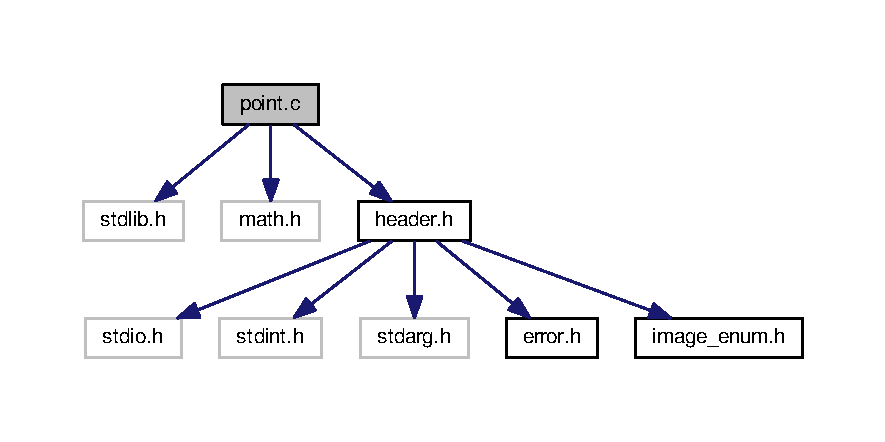
\includegraphics[width=350pt]{point_8c__incl}
\end{center}
\end{figure}
\subsection*{Functions}
\begin{DoxyCompactItemize}
\item 
\hyperlink{header_8h_a8b81d020f830e116585b833ea21410c1}{Imel\+Point} $\ast$ \hyperlink{point_8c_a20c030176364130df49237e29b69308c}{imel\+\_\+point\+\_\+new} (\hyperlink{header_8h_ad8298d38a89742ed84029b278c6acee5}{Imel\+Image} $\ast$image, \hyperlink{header_8h_af8a2b40c34eeed326846d0098ea84ec2}{Imel\+Size} x, \hyperlink{header_8h_af8a2b40c34eeed326846d0098ea84ec2}{Imel\+Size} y, \hyperlink{header_8h_add7dd9f8c093208bc4fd135a22a670ba}{Imel\+Pixel} pixel)
\begin{DoxyCompactList}\small\item\em Make a new point. \end{DoxyCompactList}\item 
void \hyperlink{point_8c_a2d4fd9ed985458d60083b5c31623b015}{imel\+\_\+point\+\_\+free} (\hyperlink{header_8h_a8b81d020f830e116585b833ea21410c1}{Imel\+Point} $\ast$point)
\begin{DoxyCompactList}\small\item\em Free the memory allocated for the point. \end{DoxyCompactList}\item 
void \hyperlink{point_8c_a64a1116a6bd2ee937316ee47f9bd7640}{imel\+\_\+point\+\_\+array\+\_\+free} (\hyperlink{header_8h_a8b81d020f830e116585b833ea21410c1}{Imel\+Point} $\ast$$\ast$points)
\begin{DoxyCompactList}\small\item\em Free the memory allocated for an array of points. \end{DoxyCompactList}\item 
\hyperlink{header_8h_a8b81d020f830e116585b833ea21410c1}{Imel\+Point} $\ast$ \hyperlink{point_8c_a43bca66a5e1544bb8ec8f5e9edb2c49f}{imel\+\_\+point\+\_\+get\+\_\+point\+\_\+from\+\_\+image} (\hyperlink{header_8h_ad8298d38a89742ed84029b278c6acee5}{Imel\+Image} $\ast$image, \hyperlink{header_8h_af8a2b40c34eeed326846d0098ea84ec2}{Imel\+Size} x, \hyperlink{header_8h_af8a2b40c34eeed326846d0098ea84ec2}{Imel\+Size} y)
\begin{DoxyCompactList}\small\item\em Get a reference point from an image. \end{DoxyCompactList}\item 
\hyperlink{header_8h_a8b81d020f830e116585b833ea21410c1}{Imel\+Point} $\ast$$\ast$ \hyperlink{point_8c_a5378c3d9ccaeb5f1325b64dd5740a072}{imel\+\_\+point\+\_\+get\+\_\+from\+\_\+line} (\hyperlink{header_8h_af8a2b40c34eeed326846d0098ea84ec2}{Imel\+Size} \+\_\+x1, \hyperlink{header_8h_af8a2b40c34eeed326846d0098ea84ec2}{Imel\+Size} \+\_\+y1, \hyperlink{header_8h_af8a2b40c34eeed326846d0098ea84ec2}{Imel\+Size} \+\_\+x2, \hyperlink{header_8h_af8a2b40c34eeed326846d0098ea84ec2}{Imel\+Size} \+\_\+y2, long int $\ast$lx, long int $\ast$ly, \hyperlink{header_8h_a3b961ca2b6e1029ab77a0951c3ae7260}{Imel\+Value} value\+\_\+type, double value)
\begin{DoxyCompactList}\small\item\em Get a line points. \end{DoxyCompactList}\item 
\hyperlink{header_8h_a8b81d020f830e116585b833ea21410c1}{Imel\+Point} $\ast$$\ast$ \hyperlink{point_8c_af6ac146e5bc39ce7aa7e1f070502b73d}{imel\+\_\+point\+\_\+get\+\_\+from\+\_\+reg\+\_\+shape} (\hyperlink{header_8h_af8a2b40c34eeed326846d0098ea84ec2}{Imel\+Size} x, \hyperlink{header_8h_af8a2b40c34eeed326846d0098ea84ec2}{Imel\+Size} y, \hyperlink{header_8h_af8a2b40c34eeed326846d0098ea84ec2}{Imel\+Size} r, long v, double start\+\_\+angle)
\begin{DoxyCompactList}\small\item\em Get a regular shape points. \end{DoxyCompactList}\item 
\hyperlink{header_8h_a8b81d020f830e116585b833ea21410c1}{Imel\+Point} $\ast$ \hyperlink{point_8c_ace24f6757914dd6eb38df140abe4cb8a}{imel\+\_\+point\+\_\+get\+\_\+darkest\+\_\+point} (\hyperlink{header_8h_ad8298d38a89742ed84029b278c6acee5}{Imel\+Image} $\ast$image)
\begin{DoxyCompactList}\small\item\em Get the darkest point of an image. \end{DoxyCompactList}\item 
\hyperlink{header_8h_a8b81d020f830e116585b833ea21410c1}{Imel\+Point} $\ast$$\ast$ \hyperlink{point_8c_a7bf05c9308f30c693a0a886dfb7c605b}{imel\+\_\+point\+\_\+get\+\_\+darkest\+\_\+points} (\hyperlink{header_8h_ad8298d38a89742ed84029b278c6acee5}{Imel\+Image} $\ast$image)
\begin{DoxyCompactList}\small\item\em Get the darkest points of an image. \end{DoxyCompactList}\item 
\hyperlink{header_8h_a8b81d020f830e116585b833ea21410c1}{Imel\+Point} $\ast$ \hyperlink{point_8c_a84c44615d1002068825cfbdf9508e2c6}{imel\+\_\+point\+\_\+get\+\_\+brightest\+\_\+point} (\hyperlink{header_8h_ad8298d38a89742ed84029b278c6acee5}{Imel\+Image} $\ast$image)
\begin{DoxyCompactList}\small\item\em Get the brightest point of an image. \end{DoxyCompactList}\item 
\hyperlink{header_8h_a8b81d020f830e116585b833ea21410c1}{Imel\+Point} $\ast$$\ast$ \hyperlink{point_8c_a821e4cca282e847f1367a23f58b7fffd}{imel\+\_\+point\+\_\+get\+\_\+brightest\+\_\+points} (\hyperlink{header_8h_ad8298d38a89742ed84029b278c6acee5}{Imel\+Image} $\ast$image)
\begin{DoxyCompactList}\small\item\em Get the brightest points of an image. \end{DoxyCompactList}\end{DoxyCompactItemize}


\subsection{Detailed Description}
This file contains functions to operate with points. 

\begin{DoxyAuthor}{Author}
Davide Francesco Merico 
\end{DoxyAuthor}


\subsection{Function Documentation}
\index{point.\+c@{point.\+c}!imel\+\_\+point\+\_\+array\+\_\+free@{imel\+\_\+point\+\_\+array\+\_\+free}}
\index{imel\+\_\+point\+\_\+array\+\_\+free@{imel\+\_\+point\+\_\+array\+\_\+free}!point.\+c@{point.\+c}}
\subsubsection[{\texorpdfstring{imel\+\_\+point\+\_\+array\+\_\+free(\+Imel\+Point $\ast$$\ast$points)}{imel_point_array_free(ImelPoint **points)}}]{\setlength{\rightskip}{0pt plus 5cm}void imel\+\_\+point\+\_\+array\+\_\+free (
\begin{DoxyParamCaption}
\item[{{\bf Imel\+Point} $\ast$$\ast$}]{points}
\end{DoxyParamCaption}
)}\hypertarget{point_8c_a64a1116a6bd2ee937316ee47f9bd7640}{}\label{point_8c_a64a1116a6bd2ee937316ee47f9bd7640}


Free the memory allocated for an array of points. 


\begin{DoxyParams}{Parameters}
{\em points} & N\+U\+L\+L-\/terminated \hyperlink{header_8h_a8b81d020f830e116585b833ea21410c1}{Imel\+Point} array \\
\hline
\end{DoxyParams}
\index{point.\+c@{point.\+c}!imel\+\_\+point\+\_\+free@{imel\+\_\+point\+\_\+free}}
\index{imel\+\_\+point\+\_\+free@{imel\+\_\+point\+\_\+free}!point.\+c@{point.\+c}}
\subsubsection[{\texorpdfstring{imel\+\_\+point\+\_\+free(\+Imel\+Point $\ast$point)}{imel_point_free(ImelPoint *point)}}]{\setlength{\rightskip}{0pt plus 5cm}void imel\+\_\+point\+\_\+free (
\begin{DoxyParamCaption}
\item[{{\bf Imel\+Point} $\ast$}]{point}
\end{DoxyParamCaption}
)}\hypertarget{point_8c_a2d4fd9ed985458d60083b5c31623b015}{}\label{point_8c_a2d4fd9ed985458d60083b5c31623b015}


Free the memory allocated for the point. 


\begin{DoxyParams}{Parameters}
{\em point} & Point to free \\
\hline
\end{DoxyParams}
\begin{DoxyNote}{Note}
Same as {\ttfamily free (point)} 
\end{DoxyNote}
\index{point.\+c@{point.\+c}!imel\+\_\+point\+\_\+get\+\_\+brightest\+\_\+point@{imel\+\_\+point\+\_\+get\+\_\+brightest\+\_\+point}}
\index{imel\+\_\+point\+\_\+get\+\_\+brightest\+\_\+point@{imel\+\_\+point\+\_\+get\+\_\+brightest\+\_\+point}!point.\+c@{point.\+c}}
\subsubsection[{\texorpdfstring{imel\+\_\+point\+\_\+get\+\_\+brightest\+\_\+point(\+Imel\+Image $\ast$image)}{imel_point_get_brightest_point(ImelImage *image)}}]{\setlength{\rightskip}{0pt plus 5cm}{\bf Imel\+Point}$\ast$ imel\+\_\+point\+\_\+get\+\_\+brightest\+\_\+point (
\begin{DoxyParamCaption}
\item[{{\bf Imel\+Image} $\ast$}]{image}
\end{DoxyParamCaption}
)}\hypertarget{point_8c_a84c44615d1002068825cfbdf9508e2c6}{}\label{point_8c_a84c44615d1002068825cfbdf9508e2c6}


Get the brightest point of an image. 


\begin{DoxyParams}{Parameters}
{\em image} & Reference image \\
\hline
\end{DoxyParams}
\begin{DoxyReturn}{Returns}
A new \hyperlink{header_8h_a8b81d020f830e116585b833ea21410c1}{Imel\+Point} type
\end{DoxyReturn}
\begin{DoxySeeAlso}{See also}
\hyperlink{point_8c_a821e4cca282e847f1367a23f58b7fffd}{imel\+\_\+point\+\_\+get\+\_\+brightest\+\_\+points} 

\hyperlink{point_8c_ace24f6757914dd6eb38df140abe4cb8a}{imel\+\_\+point\+\_\+get\+\_\+darkest\+\_\+point} 
\end{DoxySeeAlso}
\index{point.\+c@{point.\+c}!imel\+\_\+point\+\_\+get\+\_\+brightest\+\_\+points@{imel\+\_\+point\+\_\+get\+\_\+brightest\+\_\+points}}
\index{imel\+\_\+point\+\_\+get\+\_\+brightest\+\_\+points@{imel\+\_\+point\+\_\+get\+\_\+brightest\+\_\+points}!point.\+c@{point.\+c}}
\subsubsection[{\texorpdfstring{imel\+\_\+point\+\_\+get\+\_\+brightest\+\_\+points(\+Imel\+Image $\ast$image)}{imel_point_get_brightest_points(ImelImage *image)}}]{\setlength{\rightskip}{0pt plus 5cm}{\bf Imel\+Point}$\ast$$\ast$ imel\+\_\+point\+\_\+get\+\_\+brightest\+\_\+points (
\begin{DoxyParamCaption}
\item[{{\bf Imel\+Image} $\ast$}]{image}
\end{DoxyParamCaption}
)}\hypertarget{point_8c_a821e4cca282e847f1367a23f58b7fffd}{}\label{point_8c_a821e4cca282e847f1367a23f58b7fffd}


Get the brightest points of an image. 

This function return the brightest point in {\ttfamily image} and if are more then one point return a reference to all occourrence of the brightest point.


\begin{DoxyParams}{Parameters}
{\em image} & Reference image \\
\hline
\end{DoxyParams}
\begin{DoxyReturn}{Returns}
A new \hyperlink{header_8h_a8b81d020f830e116585b833ea21410c1}{Imel\+Point} type
\end{DoxyReturn}
\begin{DoxySeeAlso}{See also}
\hyperlink{point_8c_a84c44615d1002068825cfbdf9508e2c6}{imel\+\_\+point\+\_\+get\+\_\+brightest\+\_\+point} 

\hyperlink{point_8c_a7bf05c9308f30c693a0a886dfb7c605b}{imel\+\_\+point\+\_\+get\+\_\+darkest\+\_\+points} 
\end{DoxySeeAlso}
\index{point.\+c@{point.\+c}!imel\+\_\+point\+\_\+get\+\_\+darkest\+\_\+point@{imel\+\_\+point\+\_\+get\+\_\+darkest\+\_\+point}}
\index{imel\+\_\+point\+\_\+get\+\_\+darkest\+\_\+point@{imel\+\_\+point\+\_\+get\+\_\+darkest\+\_\+point}!point.\+c@{point.\+c}}
\subsubsection[{\texorpdfstring{imel\+\_\+point\+\_\+get\+\_\+darkest\+\_\+point(\+Imel\+Image $\ast$image)}{imel_point_get_darkest_point(ImelImage *image)}}]{\setlength{\rightskip}{0pt plus 5cm}{\bf Imel\+Point}$\ast$ imel\+\_\+point\+\_\+get\+\_\+darkest\+\_\+point (
\begin{DoxyParamCaption}
\item[{{\bf Imel\+Image} $\ast$}]{image}
\end{DoxyParamCaption}
)}\hypertarget{point_8c_ace24f6757914dd6eb38df140abe4cb8a}{}\label{point_8c_ace24f6757914dd6eb38df140abe4cb8a}


Get the darkest point of an image. 


\begin{DoxyParams}{Parameters}
{\em image} & Reference image \\
\hline
\end{DoxyParams}
\begin{DoxyReturn}{Returns}
A new \hyperlink{header_8h_a8b81d020f830e116585b833ea21410c1}{Imel\+Point} type
\end{DoxyReturn}
\begin{DoxySeeAlso}{See also}
\hyperlink{point_8c_a84c44615d1002068825cfbdf9508e2c6}{imel\+\_\+point\+\_\+get\+\_\+brightest\+\_\+point} 

\hyperlink{point_8c_a7bf05c9308f30c693a0a886dfb7c605b}{imel\+\_\+point\+\_\+get\+\_\+darkest\+\_\+points} 
\end{DoxySeeAlso}
\index{point.\+c@{point.\+c}!imel\+\_\+point\+\_\+get\+\_\+darkest\+\_\+points@{imel\+\_\+point\+\_\+get\+\_\+darkest\+\_\+points}}
\index{imel\+\_\+point\+\_\+get\+\_\+darkest\+\_\+points@{imel\+\_\+point\+\_\+get\+\_\+darkest\+\_\+points}!point.\+c@{point.\+c}}
\subsubsection[{\texorpdfstring{imel\+\_\+point\+\_\+get\+\_\+darkest\+\_\+points(\+Imel\+Image $\ast$image)}{imel_point_get_darkest_points(ImelImage *image)}}]{\setlength{\rightskip}{0pt plus 5cm}{\bf Imel\+Point}$\ast$$\ast$ imel\+\_\+point\+\_\+get\+\_\+darkest\+\_\+points (
\begin{DoxyParamCaption}
\item[{{\bf Imel\+Image} $\ast$}]{image}
\end{DoxyParamCaption}
)}\hypertarget{point_8c_a7bf05c9308f30c693a0a886dfb7c605b}{}\label{point_8c_a7bf05c9308f30c693a0a886dfb7c605b}


Get the darkest points of an image. 

This function return the darkest point in {\ttfamily image} and if are more then one point return a reference to all occourrence of the darkest point.


\begin{DoxyParams}{Parameters}
{\em image} & Reference image \\
\hline
\end{DoxyParams}
\begin{DoxyReturn}{Returns}
A new \hyperlink{header_8h_a8b81d020f830e116585b833ea21410c1}{Imel\+Point} type
\end{DoxyReturn}
\begin{DoxySeeAlso}{See also}
\hyperlink{point_8c_a84c44615d1002068825cfbdf9508e2c6}{imel\+\_\+point\+\_\+get\+\_\+brightest\+\_\+point} 

\hyperlink{point_8c_ace24f6757914dd6eb38df140abe4cb8a}{imel\+\_\+point\+\_\+get\+\_\+darkest\+\_\+point} 
\end{DoxySeeAlso}
\index{point.\+c@{point.\+c}!imel\+\_\+point\+\_\+get\+\_\+from\+\_\+line@{imel\+\_\+point\+\_\+get\+\_\+from\+\_\+line}}
\index{imel\+\_\+point\+\_\+get\+\_\+from\+\_\+line@{imel\+\_\+point\+\_\+get\+\_\+from\+\_\+line}!point.\+c@{point.\+c}}
\subsubsection[{\texorpdfstring{imel\+\_\+point\+\_\+get\+\_\+from\+\_\+line(\+Imel\+Size \+\_\+x1, Imel\+Size \+\_\+y1, Imel\+Size \+\_\+x2, Imel\+Size \+\_\+y2, long int $\ast$lx, long int $\ast$ly, Imel\+Value value\+\_\+type, double value)}{imel_point_get_from_line(ImelSize _x1, ImelSize _y1, ImelSize _x2, ImelSize _y2, long int *lx, long int *ly, ImelValue value_type, double value)}}]{\setlength{\rightskip}{0pt plus 5cm}{\bf Imel\+Point}$\ast$$\ast$ imel\+\_\+point\+\_\+get\+\_\+from\+\_\+line (
\begin{DoxyParamCaption}
\item[{{\bf Imel\+Size}}]{\+\_\+x1, }
\item[{{\bf Imel\+Size}}]{\+\_\+y1, }
\item[{{\bf Imel\+Size}}]{\+\_\+x2, }
\item[{{\bf Imel\+Size}}]{\+\_\+y2, }
\item[{long int $\ast$}]{lx, }
\item[{long int $\ast$}]{ly, }
\item[{{\bf Imel\+Value}}]{value\+\_\+type, }
\item[{double}]{value}
\end{DoxyParamCaption}
)}\hypertarget{point_8c_a5378c3d9ccaeb5f1325b64dd5740a072}{}\label{point_8c_a5378c3d9ccaeb5f1325b64dd5740a072}


Get a line points. 

This function get all points in the line from coordinate $(\_x_1,\_y_1)$ to coordinate $(\_x_2,\_y_2)$. You can get the line width and height respectively from {\ttfamily lx} and {\ttfamily ly} argument.


\begin{DoxyParams}{Parameters}
{\em \+\_\+x1} & Start line x coordinate \\
\hline
{\em \+\_\+y1} & Start line y coordinate \\
\hline
{\em \+\_\+x2} & End line x coordinate \\
\hline
{\em \+\_\+y2} & End line y coordinate \\
\hline
{\em lx} & N\+U\+LL or if passed, this function put inside it the line width \\
\hline
{\em ly} & N\+U\+LL or if passed, this function put inside it the line height \\
\hline
{\em value\+\_\+type} & Type of value passed as {\ttfamily value} \\
\hline
{\em value} & Number of points you want to get from the line. The points will be uniformely distributed. \\
\hline
\end{DoxyParams}
\begin{DoxyReturn}{Returns}
A N\+U\+L\+L-\/terminated array with the line points.
\end{DoxyReturn}
\begin{DoxySeeAlso}{See also}
\hyperlink{header_8h_a3b961ca2b6e1029ab77a0951c3ae7260}{Imel\+Value} 

\hyperlink{point_8c_a64a1116a6bd2ee937316ee47f9bd7640}{imel\+\_\+point\+\_\+array\+\_\+free} 
\end{DoxySeeAlso}
\index{point.\+c@{point.\+c}!imel\+\_\+point\+\_\+get\+\_\+from\+\_\+reg\+\_\+shape@{imel\+\_\+point\+\_\+get\+\_\+from\+\_\+reg\+\_\+shape}}
\index{imel\+\_\+point\+\_\+get\+\_\+from\+\_\+reg\+\_\+shape@{imel\+\_\+point\+\_\+get\+\_\+from\+\_\+reg\+\_\+shape}!point.\+c@{point.\+c}}
\subsubsection[{\texorpdfstring{imel\+\_\+point\+\_\+get\+\_\+from\+\_\+reg\+\_\+shape(\+Imel\+Size x, Imel\+Size y, Imel\+Size r, long v, double start\+\_\+angle)}{imel_point_get_from_reg_shape(ImelSize x, ImelSize y, ImelSize r, long v, double start_angle)}}]{\setlength{\rightskip}{0pt plus 5cm}{\bf Imel\+Point}$\ast$$\ast$ imel\+\_\+point\+\_\+get\+\_\+from\+\_\+reg\+\_\+shape (
\begin{DoxyParamCaption}
\item[{{\bf Imel\+Size}}]{x, }
\item[{{\bf Imel\+Size}}]{y, }
\item[{{\bf Imel\+Size}}]{r, }
\item[{long}]{v, }
\item[{double}]{start\+\_\+angle}
\end{DoxyParamCaption}
)}\hypertarget{point_8c_af6ac146e5bc39ce7aa7e1f070502b73d}{}\label{point_8c_af6ac146e5bc39ce7aa7e1f070502b73d}


Get a regular shape points. 

This function get the points from a regular shape with center in coordinate $(x,y)$, {\ttfamily r} radius, {\ttfamily v} vertices and an angle of {\ttfamily start} angle.


\begin{DoxyParams}{Parameters}
{\em x} & Center x coordinate \\
\hline
{\em y} & Center y coordinate \\
\hline
{\em r} & Radius \\
\hline
{\em v} & Vertices \\
\hline
{\em start\+\_\+angle} & Start angle in radians \\
\hline
\end{DoxyParams}
\begin{DoxyReturn}{Returns}
A N\+U\+L\+L-\/terminated array with the regular shape points
\end{DoxyReturn}
\begin{DoxySeeAlso}{See also}
\hyperlink{point_8c_a64a1116a6bd2ee937316ee47f9bd7640}{imel\+\_\+point\+\_\+array\+\_\+free} 

\hyperlink{header_8h_adff9f86a929b90364f856932fc5e064f}{R\+A\+D\+\_\+\+T\+O\+\_\+\+D\+EG} 

\hyperlink{header_8h_a0978c9c7420f81adda347a7c6d22f085}{D\+E\+G\+\_\+\+T\+O\+\_\+\+R\+AD} 
\end{DoxySeeAlso}
\index{point.\+c@{point.\+c}!imel\+\_\+point\+\_\+get\+\_\+point\+\_\+from\+\_\+image@{imel\+\_\+point\+\_\+get\+\_\+point\+\_\+from\+\_\+image}}
\index{imel\+\_\+point\+\_\+get\+\_\+point\+\_\+from\+\_\+image@{imel\+\_\+point\+\_\+get\+\_\+point\+\_\+from\+\_\+image}!point.\+c@{point.\+c}}
\subsubsection[{\texorpdfstring{imel\+\_\+point\+\_\+get\+\_\+point\+\_\+from\+\_\+image(\+Imel\+Image $\ast$image, Imel\+Size x, Imel\+Size y)}{imel_point_get_point_from_image(ImelImage *image, ImelSize x, ImelSize y)}}]{\setlength{\rightskip}{0pt plus 5cm}{\bf Imel\+Point}$\ast$ imel\+\_\+point\+\_\+get\+\_\+point\+\_\+from\+\_\+image (
\begin{DoxyParamCaption}
\item[{{\bf Imel\+Image} $\ast$}]{image, }
\item[{{\bf Imel\+Size}}]{x, }
\item[{{\bf Imel\+Size}}]{y}
\end{DoxyParamCaption}
)}\hypertarget{point_8c_a43bca66a5e1544bb8ec8f5e9edb2c49f}{}\label{point_8c_a43bca66a5e1544bb8ec8f5e9edb2c49f}


Get a reference point from an image. 


\begin{DoxyParams}{Parameters}
{\em image} & Reference image \\
\hline
{\em x} & Point x coordinate \\
\hline
{\em y} & Point y coordinate \\
\hline
\end{DoxyParams}
\begin{DoxyReturn}{Returns}
A new \hyperlink{header_8h_a8b81d020f830e116585b833ea21410c1}{Imel\+Point} type with a pixel set equal to the image pixel at coordinate $(x,y)$. 
\end{DoxyReturn}
\index{point.\+c@{point.\+c}!imel\+\_\+point\+\_\+new@{imel\+\_\+point\+\_\+new}}
\index{imel\+\_\+point\+\_\+new@{imel\+\_\+point\+\_\+new}!point.\+c@{point.\+c}}
\subsubsection[{\texorpdfstring{imel\+\_\+point\+\_\+new(\+Imel\+Image $\ast$image, Imel\+Size x, Imel\+Size y, Imel\+Pixel pixel)}{imel_point_new(ImelImage *image, ImelSize x, ImelSize y, ImelPixel pixel)}}]{\setlength{\rightskip}{0pt plus 5cm}{\bf Imel\+Point}$\ast$ imel\+\_\+point\+\_\+new (
\begin{DoxyParamCaption}
\item[{{\bf Imel\+Image} $\ast$}]{image, }
\item[{{\bf Imel\+Size}}]{x, }
\item[{{\bf Imel\+Size}}]{y, }
\item[{{\bf Imel\+Pixel}}]{pixel}
\end{DoxyParamCaption}
)}\hypertarget{point_8c_a20c030176364130df49237e29b69308c}{}\label{point_8c_a20c030176364130df49237e29b69308c}


Make a new point. 

This function makes a point at coordinate $(x,y)\in image$ with a chosen color and level.


\begin{DoxyParams}{Parameters}
{\em image} & Reference image \\
\hline
{\em x} & Point x coordinate \\
\hline
{\em y} & Point y coordinate \\
\hline
{\em pixel} & Point color and level \\
\hline
\end{DoxyParams}
\begin{DoxyReturn}{Returns}
A new \hyperlink{header_8h_a8b81d020f830e116585b833ea21410c1}{Imel\+Point} type or N\+U\+LL on error 
\end{DoxyReturn}

\hypertarget{value_8c}{}\section{value.\+c File Reference}
\label{value_8c}\index{value.\+c@{value.\+c}}


This file contains functions to convert values.  


{\ttfamily \#include \char`\"{}header.\+h\char`\"{}}\\*
Include dependency graph for value.\+c\+:
\nopagebreak
\begin{figure}[H]
\begin{center}
\leavevmode
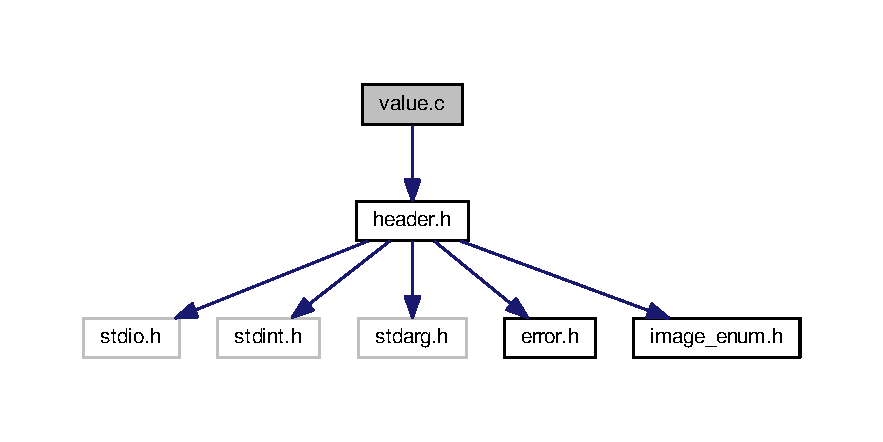
\includegraphics[width=350pt]{value_8c__incl}
\end{center}
\end{figure}
\subsection*{Functions}
\begin{DoxyCompactItemize}
\item 
double \hyperlink{value_8c_a8fd8fa1742f7d9d8fdeddfe8b913af98}{imel\+\_\+value\+\_\+percentage\+\_\+to\+\_\+generic} (double value, double opt\+\_\+value)
\item 
double \hyperlink{value_8c_a0d421a94b5a7de0a78b2cc0d9917755d}{imel\+\_\+value\+\_\+pixel\+\_\+to\+\_\+percentage} (double value, double opt\+\_\+value)
\item 
double \hyperlink{value_8c_a09670d688bb50c3334e933772839fb23}{imel\+\_\+value\+\_\+convert} (\hyperlink{header_8h_a3b961ca2b6e1029ab77a0951c3ae7260}{Imel\+Value} from\+\_\+value, double value, \hyperlink{header_8h_a3b961ca2b6e1029ab77a0951c3ae7260}{Imel\+Value} to\+\_\+value,...)
\begin{DoxyCompactList}\small\item\em Convert a value in another one. \end{DoxyCompactList}\end{DoxyCompactItemize}


\subsection{Detailed Description}
This file contains functions to convert values. 

\begin{DoxyAuthor}{Author}
Davide Francesco Merico 
\end{DoxyAuthor}


\subsection{Function Documentation}
\index{value.\+c@{value.\+c}!imel\+\_\+value\+\_\+convert@{imel\+\_\+value\+\_\+convert}}
\index{imel\+\_\+value\+\_\+convert@{imel\+\_\+value\+\_\+convert}!value.\+c@{value.\+c}}
\subsubsection[{\texorpdfstring{imel\+\_\+value\+\_\+convert(\+Imel\+Value from\+\_\+value, double value, Imel\+Value to\+\_\+value,...)}{imel_value_convert(ImelValue from_value, double value, ImelValue to_value,...)}}]{\setlength{\rightskip}{0pt plus 5cm}double imel\+\_\+value\+\_\+convert (
\begin{DoxyParamCaption}
\item[{{\bf Imel\+Value}}]{from\+\_\+value, }
\item[{double}]{value, }
\item[{{\bf Imel\+Value}}]{to\+\_\+value, }
\item[{}]{...}
\end{DoxyParamCaption}
)}\hypertarget{value_8c_a09670d688bb50c3334e933772839fb23}{}\label{value_8c_a09670d688bb50c3334e933772839fb23}


Convert a value in another one. 


\begin{DoxyParams}{Parameters}
{\em from\+\_\+value} & Type of value you to convert in {\ttfamily to\+\_\+value} \\
\hline
{\em value} & Value to convert in {\ttfamily to\+\_\+value} \\
\hline
{\em to\+\_\+value} & Type of value to convert from {\ttfamily from\+\_\+value} \\
\hline
{\em ...} & Value to convert from {\ttfamily from\+\_\+value} \\
\hline
\end{DoxyParams}
\begin{DoxyReturn}{Returns}
Value converted 
\end{DoxyReturn}
\index{value.\+c@{value.\+c}!imel\+\_\+value\+\_\+percentage\+\_\+to\+\_\+generic@{imel\+\_\+value\+\_\+percentage\+\_\+to\+\_\+generic}}
\index{imel\+\_\+value\+\_\+percentage\+\_\+to\+\_\+generic@{imel\+\_\+value\+\_\+percentage\+\_\+to\+\_\+generic}!value.\+c@{value.\+c}}
\subsubsection[{\texorpdfstring{imel\+\_\+value\+\_\+percentage\+\_\+to\+\_\+generic(double value, double opt\+\_\+value)}{imel_value_percentage_to_generic(double value, double opt_value)}}]{\setlength{\rightskip}{0pt plus 5cm}double imel\+\_\+value\+\_\+percentage\+\_\+to\+\_\+generic (
\begin{DoxyParamCaption}
\item[{double}]{value, }
\item[{double}]{opt\+\_\+value}
\end{DoxyParamCaption}
)}\hypertarget{value_8c_a8fd8fa1742f7d9d8fdeddfe8b913af98}{}\label{value_8c_a8fd8fa1742f7d9d8fdeddfe8b913af98}
Convert a percentage in a generic value


\begin{DoxyParams}{Parameters}
{\em value} & Percentage value \\
\hline
{\em opt\+\_\+value} & Generic value equal to 100\% \\
\hline
\end{DoxyParams}
\begin{DoxyReturn}{Returns}
Percentage value converted 
\end{DoxyReturn}
\index{value.\+c@{value.\+c}!imel\+\_\+value\+\_\+pixel\+\_\+to\+\_\+percentage@{imel\+\_\+value\+\_\+pixel\+\_\+to\+\_\+percentage}}
\index{imel\+\_\+value\+\_\+pixel\+\_\+to\+\_\+percentage@{imel\+\_\+value\+\_\+pixel\+\_\+to\+\_\+percentage}!value.\+c@{value.\+c}}
\subsubsection[{\texorpdfstring{imel\+\_\+value\+\_\+pixel\+\_\+to\+\_\+percentage(double value, double opt\+\_\+value)}{imel_value_pixel_to_percentage(double value, double opt_value)}}]{\setlength{\rightskip}{0pt plus 5cm}double imel\+\_\+value\+\_\+pixel\+\_\+to\+\_\+percentage (
\begin{DoxyParamCaption}
\item[{double}]{value, }
\item[{double}]{opt\+\_\+value}
\end{DoxyParamCaption}
)}\hypertarget{value_8c_a0d421a94b5a7de0a78b2cc0d9917755d}{}\label{value_8c_a0d421a94b5a7de0a78b2cc0d9917755d}
Convert a pixel value to percentage


\begin{DoxyParams}{Parameters}
{\em value} & Value to convert \\
\hline
{\em opt\+\_\+value} & Generic value equal to 100\% \\
\hline
\end{DoxyParams}
\begin{DoxyReturn}{Returns}
Value converted 
\end{DoxyReturn}

%--- End generated contents ---

% Index
\backmatter
\newpage
\phantomsection
\clearemptydoublepage
\addcontentsline{toc}{chapter}{Index}
\printindex

\end{document}
